\documentclass{article}
\usepackage[margin=0.5in,bottom=1in,top=1in]{geometry}
%Attempt to make changes and see if git registers.
% header formatting
\usepackage{fancyhdr}

% For drawing chemical structures 
\usepackage{chemfig}
\usepackage{xcolor}
\usepackage{twoopt}
\usepackage{ifmtarg}

\usepackage{gensymb}
 
\pagestyle{fancy}
\fancyhf{}
\fancyhead[LE,RO]{Michael Yao}
\fancyhead[RE,LO]{MCAT Study Guide, SU2019}
\fancyfoot[CE,CO]{\leftmark}
\fancyfoot[LE,RO]{\thepage}

\renewcommand{\headrulewidth}{0.75pt}
\renewcommand{\footrulewidth}{0.75pt}

\usepackage[version=4]{mhchem}
\def\ZZ#1{\global\setbondstyle{thick,color=#1}\gdef\printatom##1{\color{#1}\ensuremath{\mathrm{##1}}}}
\def\paren#1{\rlap{\kern-.75em$\left(\vrule height1ex width0pt depth1ex\vrule height0pt width2.5em depth0pt\right)_{\!#1}$}}
\definesubmol\NN{-[,,,,draw=none]}
% atom numbers (used when option atom-numbers is selected)
\newcommand{\mcfatomno}[1]{\raisebox{2pt}{\color{blue}{\ensuremath{\mathsf{_{#1}}}}}}
\definesubmol\Red{(!\NN\ZZ{red})}
\definesubmol\Green{(!\NN\ZZ{green!40!black})}
\definesubmol\Purple{(!\NN\ZZ{purple})}
\definesubmol\Black{(!\NN\ZZ{black})}
%\setatomsep{2em}\setbondstyle{thick}

% math packages
\usepackage{mathtools}
\usepackage{amsmath}
\usepackage{amssymb}    % Math symbols such as \mathbb
\newcommand{\dbar}{{\mathchar '26\mkern -12mud}}
\usepackage{bbm}
\usepackage{gensymb}
\usepackage{amsthm}
\usepackage{pgfplots}   % plots
\usepackage{pbsi}
\usepackage[T1]{fontenc}

% other packages
\usepackage{graphicx}
\graphicspath{ {../assets/} }
\usepackage{enumitem}
\usepackage{color}
\usepackage{hyperref}
\hypersetup{
    colorlinks=true,
    linktoc=all,     %set to all if you want both sections and subsections linked
    linkcolor=blue,
}

% proper inline math display, adjust height for symbols like \sum
\everymath{\displaystyle}

% define tags for math use..
\theoremstyle{plain}% default
\newtheorem{theorem}{Theorem}[section]
\newtheorem{corollary}{Corollary}[theorem]

\theoremstyle{definition}
\newtheorem{defn}{Definition}[section]
\newtheorem{proposition}{Proposition}[defn]
\newtheorem{exmp}{Example}[section]

\theoremstyle{remark}
\newtheorem*{rem}{Remark}
\newtheorem*{note}{Note}
\newtheorem{case}{Case}

% Gives begin{solution} same formating as \begin{proof}
\newenvironment{solution}
  {\begin{proof}[Solution]}
  {\end{proof}}


%running fraction with slash - requires math mode.
\newcommand*\rfrac[2]{{}^{#1}\!/_{#2}}
%shortcut to mathbb
\newcommand{\N}{\mathbb{N}}
\newcommand{\R}{\mathbb{R}}
\newcommand{\C}{\mathbb{C}}
% color highlighting
\newcommand{\hilight}[1]{\colorbox{yellow}{#1}}

\title{\vspace{-6ex}MCAT Study Guide, SU2019}
\author{Michael Yao}
\date{\today\vspace{-4ex}}

\begin{document}

\tableofcontents
\newpage

\section{Biology\textemdash Physiology}
\subsection{Types of Tissues}
The digestive system is essentially a gastrointestinal canal that is suspended within a body cavity referred to as the \textbf{coelom}; this coelom is separated into a \textbf{thoracic cavity} (upper, with the lungs and heart) and an \textbf{abdominal cavity} (lower, with the liver, stomach, and intestines). There are several types of tissue that you should know about:
\begin{enumerate}
	\item \textbf{Epithelial Tissues:} Epithelial tissue can be divided into two categories: simple (single layer of cells) and stratified (multiple layers of cells). In these categories, the epithelial cells come in a variety of shapes and sizes: squamous (flat), cuboidal, and columnar. In the gastrointestinal system, simple epithelial cells have projections called microvilli on the lumenal (also apical) side. They also have a basal lamina on the basal side that helps hold together epithelial cells using desmosomes. Tight junctions act as permeability barriers and help maintain important gradients for the digestive track. Gap junctions provide a means for water-soluble molecules to pass from the cytoplasm of one cell to the cytoplasm of another cell. If a cell secretes a substance into the lumen by way of a duct, it is referred to as an \textbf{exocrine gland}. \textbf{Endocrine glands} secrete substances into the blood. Stratified squamous epithelium usually have a protective function. \textbf{Fig. \ref{epithelial}} shows some examples of the types of epithelial tissue.
	\item \textbf{Connective Tissues:} Connective tissues include structural, blood cells, mast cells adipose cells, and melanocytes. \textbf{Fibroblasts} help secrete the proteins that make up structural connective tissue, such as \textbf{collagen} (insoluble, fibrous, strong, flexible), \textbf{reticulin} (tin fiber in spleen and lymph nodes), and \textbf{elastin} (highly cross-linked fiber associated with organs that require elasticity, like the lungs, skin, and blood vessels). \textbf{Cartilage} is secreted by \textbf{chondrocytes}, which are a specialized type of fibroblast cell. \textbf{Bone} is also a structural connective tissue, made up of collagen, calcium phosphate, and calcium carbonate. Collagen found in bond matrix is secreted by \textbf{osteoblasts}, which are specialized fibroblasts. Collagen gives bone flexbility, while the inorganic calcium-based crystals lend rigidity. The central cavity of bone has spongy \textbf{bone marrow} where RBCs and WBCs are formed. \textbf{Mast cells} can be found in the respiratory tract and GI tract, and they release \textbf{histamines} in response to allergic reactions, infections, or injuries. Histamines cause an increase in blood flow to the blood vessels of the affected region. \textbf{Adipose cells} are cells that store fat where \textbf{Melanocytes} are cells which store pigments.
	\item \textbf{Muscle Tissues:} Skeletal muscle is a voluntary muscle, while cardiac and smooth muscle are examples of involuntary muscles.
	\item \textbf{Nervous Tissues:} Nerve cells (i.e. \textbf{neurons}) are the basic structural unit that make up the nervous system. The major anatomical features are the cell body, \textbf{dendrites}, and \textbf{axon}. When a neuron becomes excited and receives electrical information, the cell body transmits the signal down the axon in the form of an action potential. The signal causes the release of a chemical neurotransmitter that diffuses across the synaptic cleft and induces an identical action potential in an adjoining neuron, muscle cell, or gland cell. This junction between two such cells is called a \textbf{synapse}.
\end{enumerate} 
\begin{figure}[!ht]
\centering
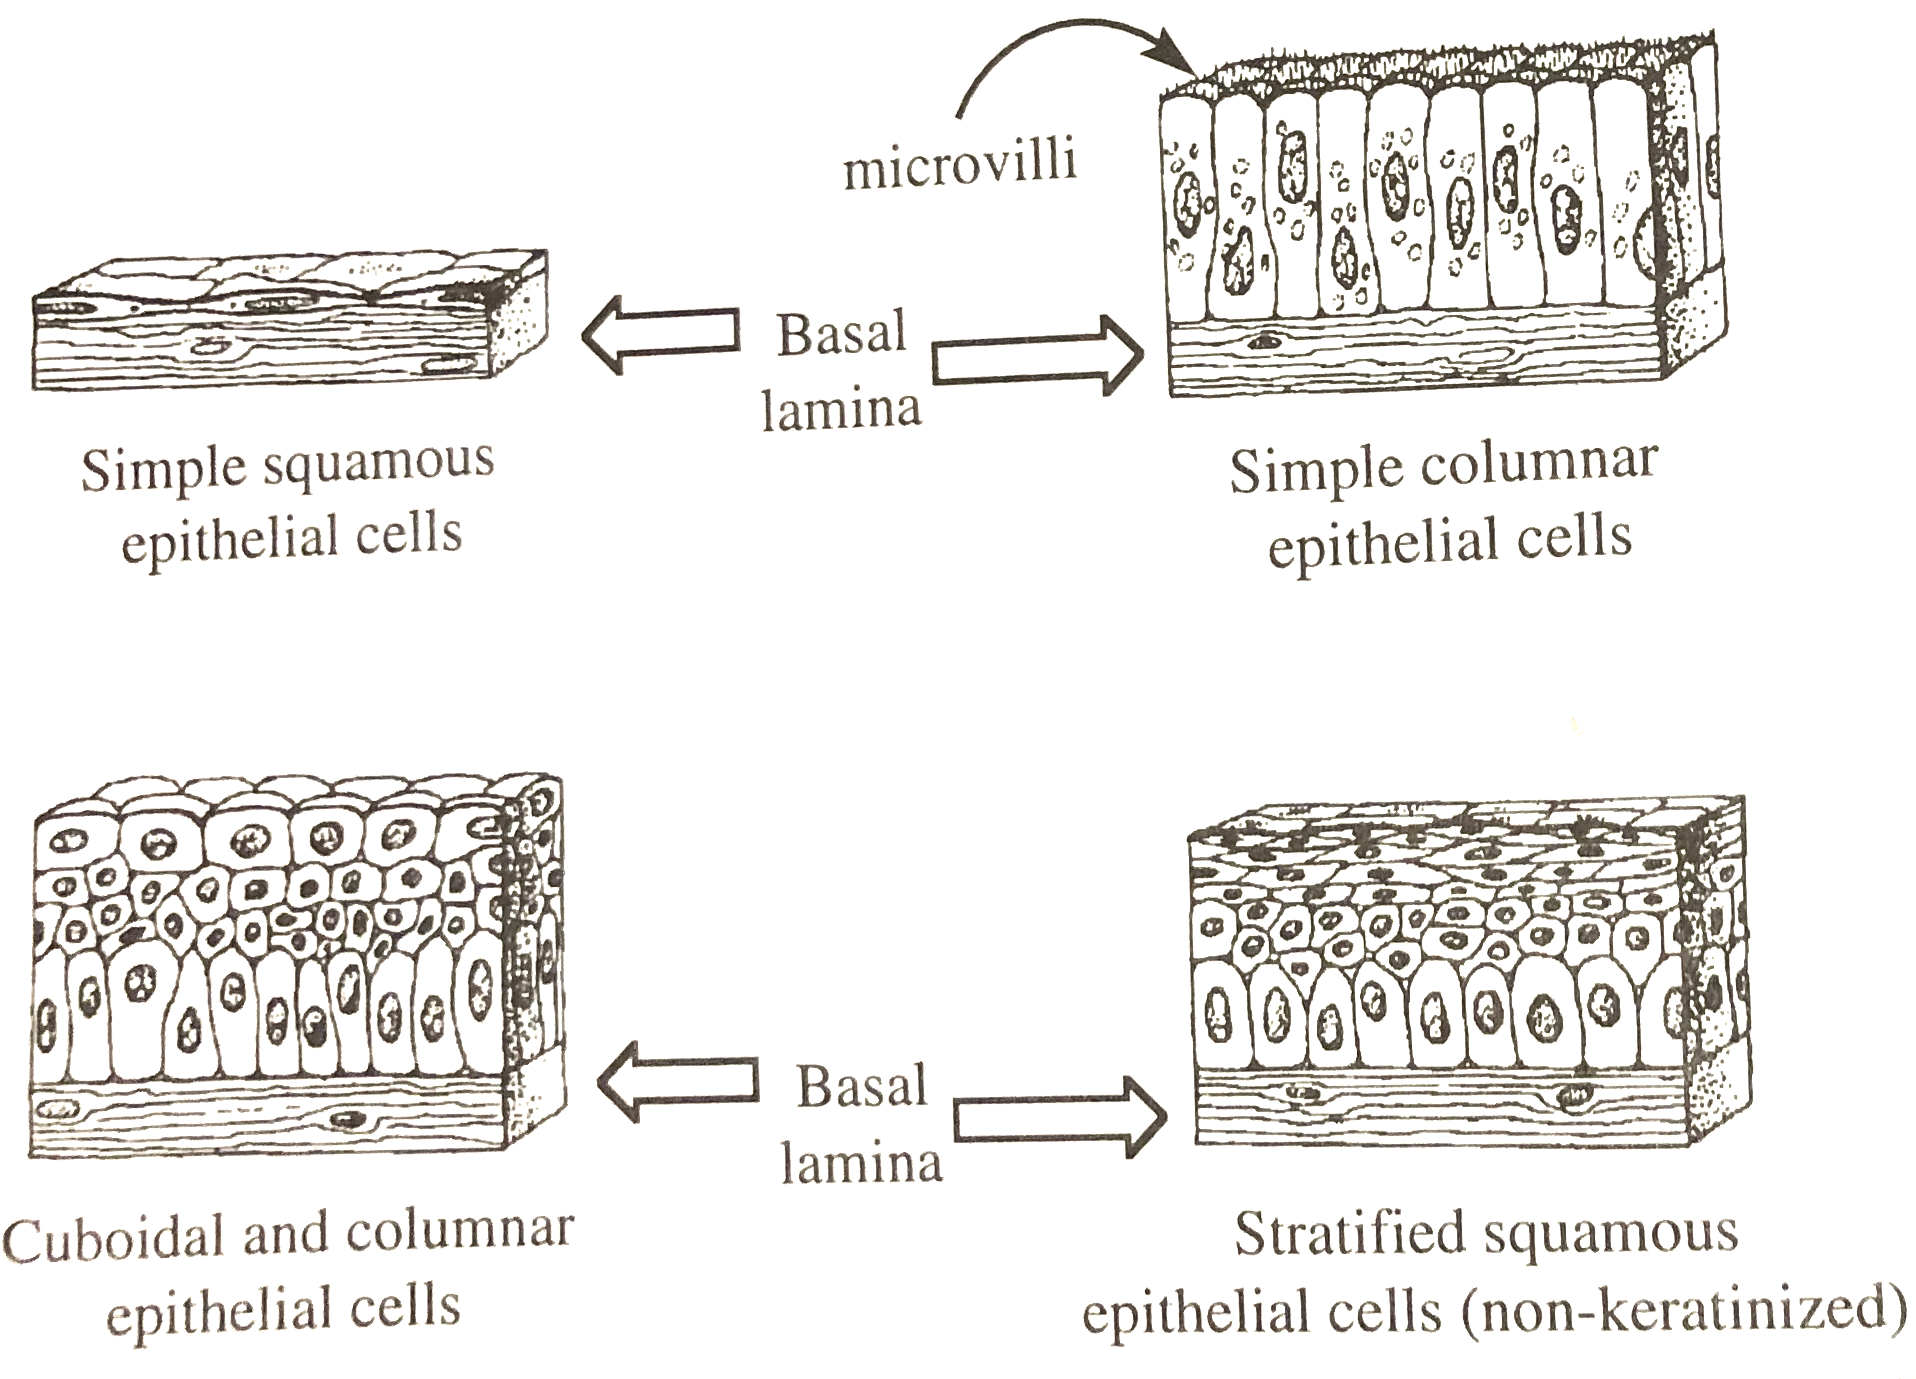
\includegraphics[width=0.7\textwidth]{epithelial.png} \label{epithelial}
\caption{Types of epithelial cells.}
\end{figure}
\indent \textbf{Skin} consists of many layers. The \textbf{epidermal} region contains \textbf{stratified epithelial cells} for protection. Below the epidermis is the \textbf{dermix} with a variety oa structures. Surrounding the hair follicles are \textbf{erector muscles}, which act to straighten the hair shaft. Below the dermis is the \textbf{subcutaneous tissue}. This is where one finds adipose deposits.\\
\indent The inside of the cell is more negatively charged with respect to the outside of the cell. This sets up a voltage that is positive on the outside of the cell. We can calculate the \textbf{membrane voltage} (i.e. potential difference) across the cell's membrane using the \textbf{Nernst equation}:
\begin{equation}
\begin{split}
V_{io}=2.3\frac{RT}{ZF}\log\left(\frac{\left[X\right]_o}{\left[X\right]_i}\right)
\end{split}
\end{equation}
\noindent where $V$ is the voltage in millivolts, $i$ refers to inside, $o$ refers to outside, $Z$ is the ion's valance, and $F$ is Faraday's constant. The inside of a neuron registers a potential difference of about \textbf{-80 mV}. 

\subsection{Action Potentials}
Stimulating a nerve causes the membrane to be \textbf{depolarized}. If the stimulus is strong enough and the depolarization exceeds the \textbf{threshold potential}, then within milliseconds, a burst of \ce{Na+} ions enters and generates an action potential. One millisecond after the burst of \ce{Na+} into the cell, the ion channels that let \ce{Na+} into the cell close and become temporarily inactive\textemdash this is referred to the \textbf{refractory period}, which lasts for several milliseconds. During this time a neuron will not be able to generate another action potential, because the \ce{Na+} channels cannot open to allow the cell membrane to depolarize.\\
\indent Once the \ce{Na+} channels have closed, the \ce{K+} channels begin to open and \ce{K+} begins to leave the cell\textemdash this is referred to as repolarization. The overshoot due to the massive outflux of \ce{K+} ions is called \textbf{hyperpolarization}. The generation of an action potential is said to be an \textbf{all-or-none} phenomenon; an example of a typical action potential is shown in \textbf{Fig. \ref{action_potential}}. \\
\begin{figure}[!ht]
\centering
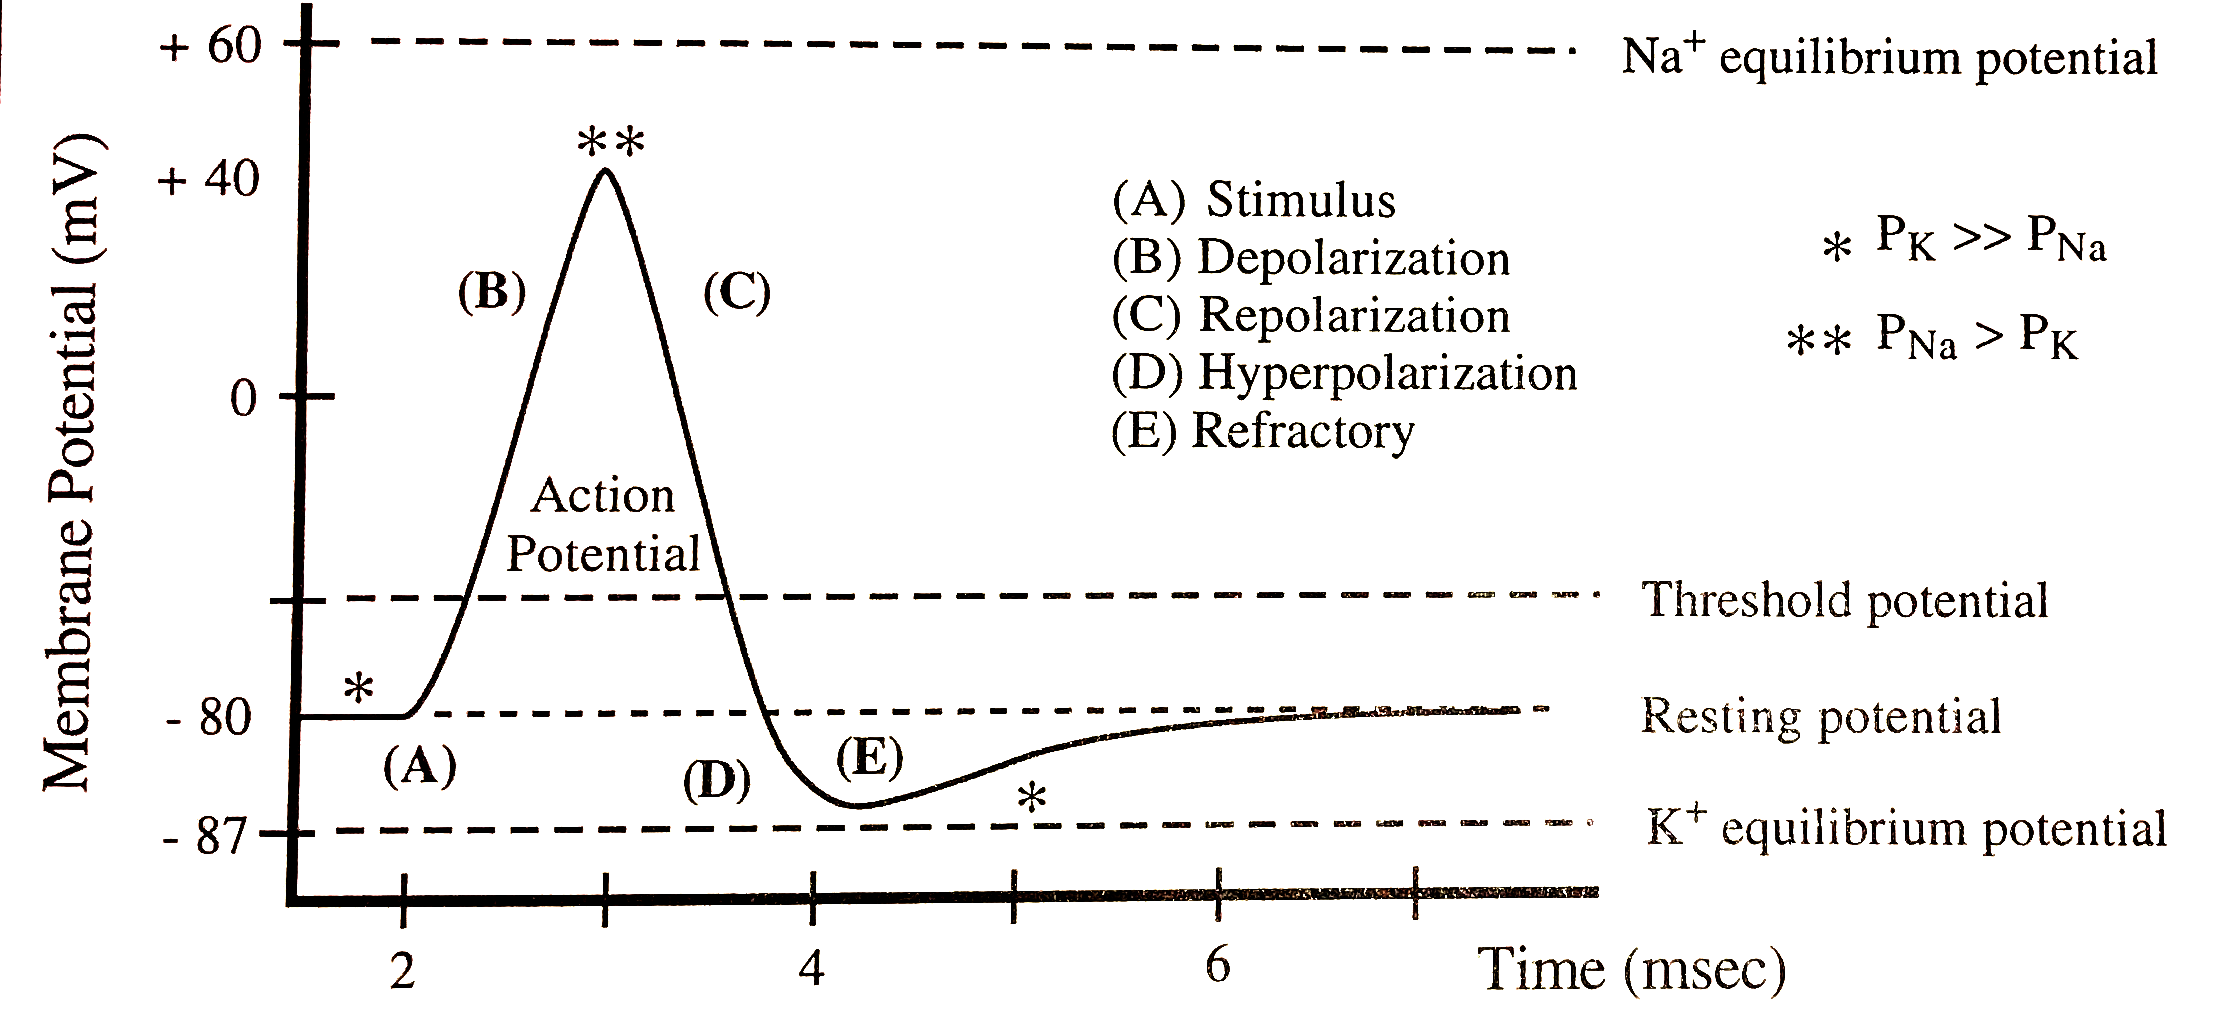
\includegraphics[width=0.7\textwidth]{action_potential.png} \label{action_potential}
\caption{A typical action potential. $P_K$ is the cell's permeability to \ce{K+} and $P_{Na}$ is the cell's permeability to \ce{Na+}.}
\end{figure}
\indent Larger diameter neurons will conduct an action potential further and faster than a small diameter neuron. This means that the ability of a neuron to conduct a current depends on the cross-sectional area of that neuron. \\
\indent \textbf{Myelinated} nerves have the ability to greatly increase the rate at which action potentials are conducted. This is because myelin acts as an electrical insulator and prevents the transfer of ions across the plasma membrane of the axon. This allows the nerve impulse to `jump' from node to node along the axon, referred to as \textbf{saltatory conduction}. \textbf{Glial cells} attach themselves to a section of an unmyelinated axon and begin to rotate around that axon to deposit a myelin sheath. The deposition of myelin along the axon is interrupted by areas where there is no myelin, called the \textbf{nodes of Ranvier}. Glial cells in the central nervous system (CNS) are called \textbf{oligodendrocytes}, while glial cells in the peripheral nervous system (PNS) are called \textbf{Schwann cells}. The CNS is made up of the brain and spinal cord while the \textbf{peripheral nervous system} represents the nerves in the periphery. 

\subsection{The Neuromuscular Junction}
At the end of the axon is a specialized area called the \textbf{terminal bouton}. Neuromuscular junctions involve a terminal bouton with hundreds of thousands of \textbf{synaptic vesicles} that contain the excitatory neurotransmitter \textbf{acetylcholine (ACh)}, which is synthesized in the cytosol of the neuron from the molecules \textbf{acetyl-CoA} and \textbf{choline}. As the action potential reaches the terminal bouton, it triggers the opening of \ce{Ca^2+} channels that generate a transient influx of \ce{Ca^2+} into the terminal region, which causes synaptic vesicles to fuse with the presynaptic membrane and release ACh into the synaptic cleft via exocytosis. \ce{Ca^2+} is pumped out of the cytosol and back into the extracellular fluid. ACh then binds to specific postsynaptic membrane receptors, which conformationally changes the ionphore channel receptor so that it can let ions like \ce{Na+} through. As \ce{Na+} enters the postsynaptic membrane, the muscle fiber begins to depolarize and an action potential is eventually generated. A diagram of the neuromuscular junction is shown in \textbf{Fig. \ref{neuromuscular}}. \\
\begin{figure}[!ht]
\centering
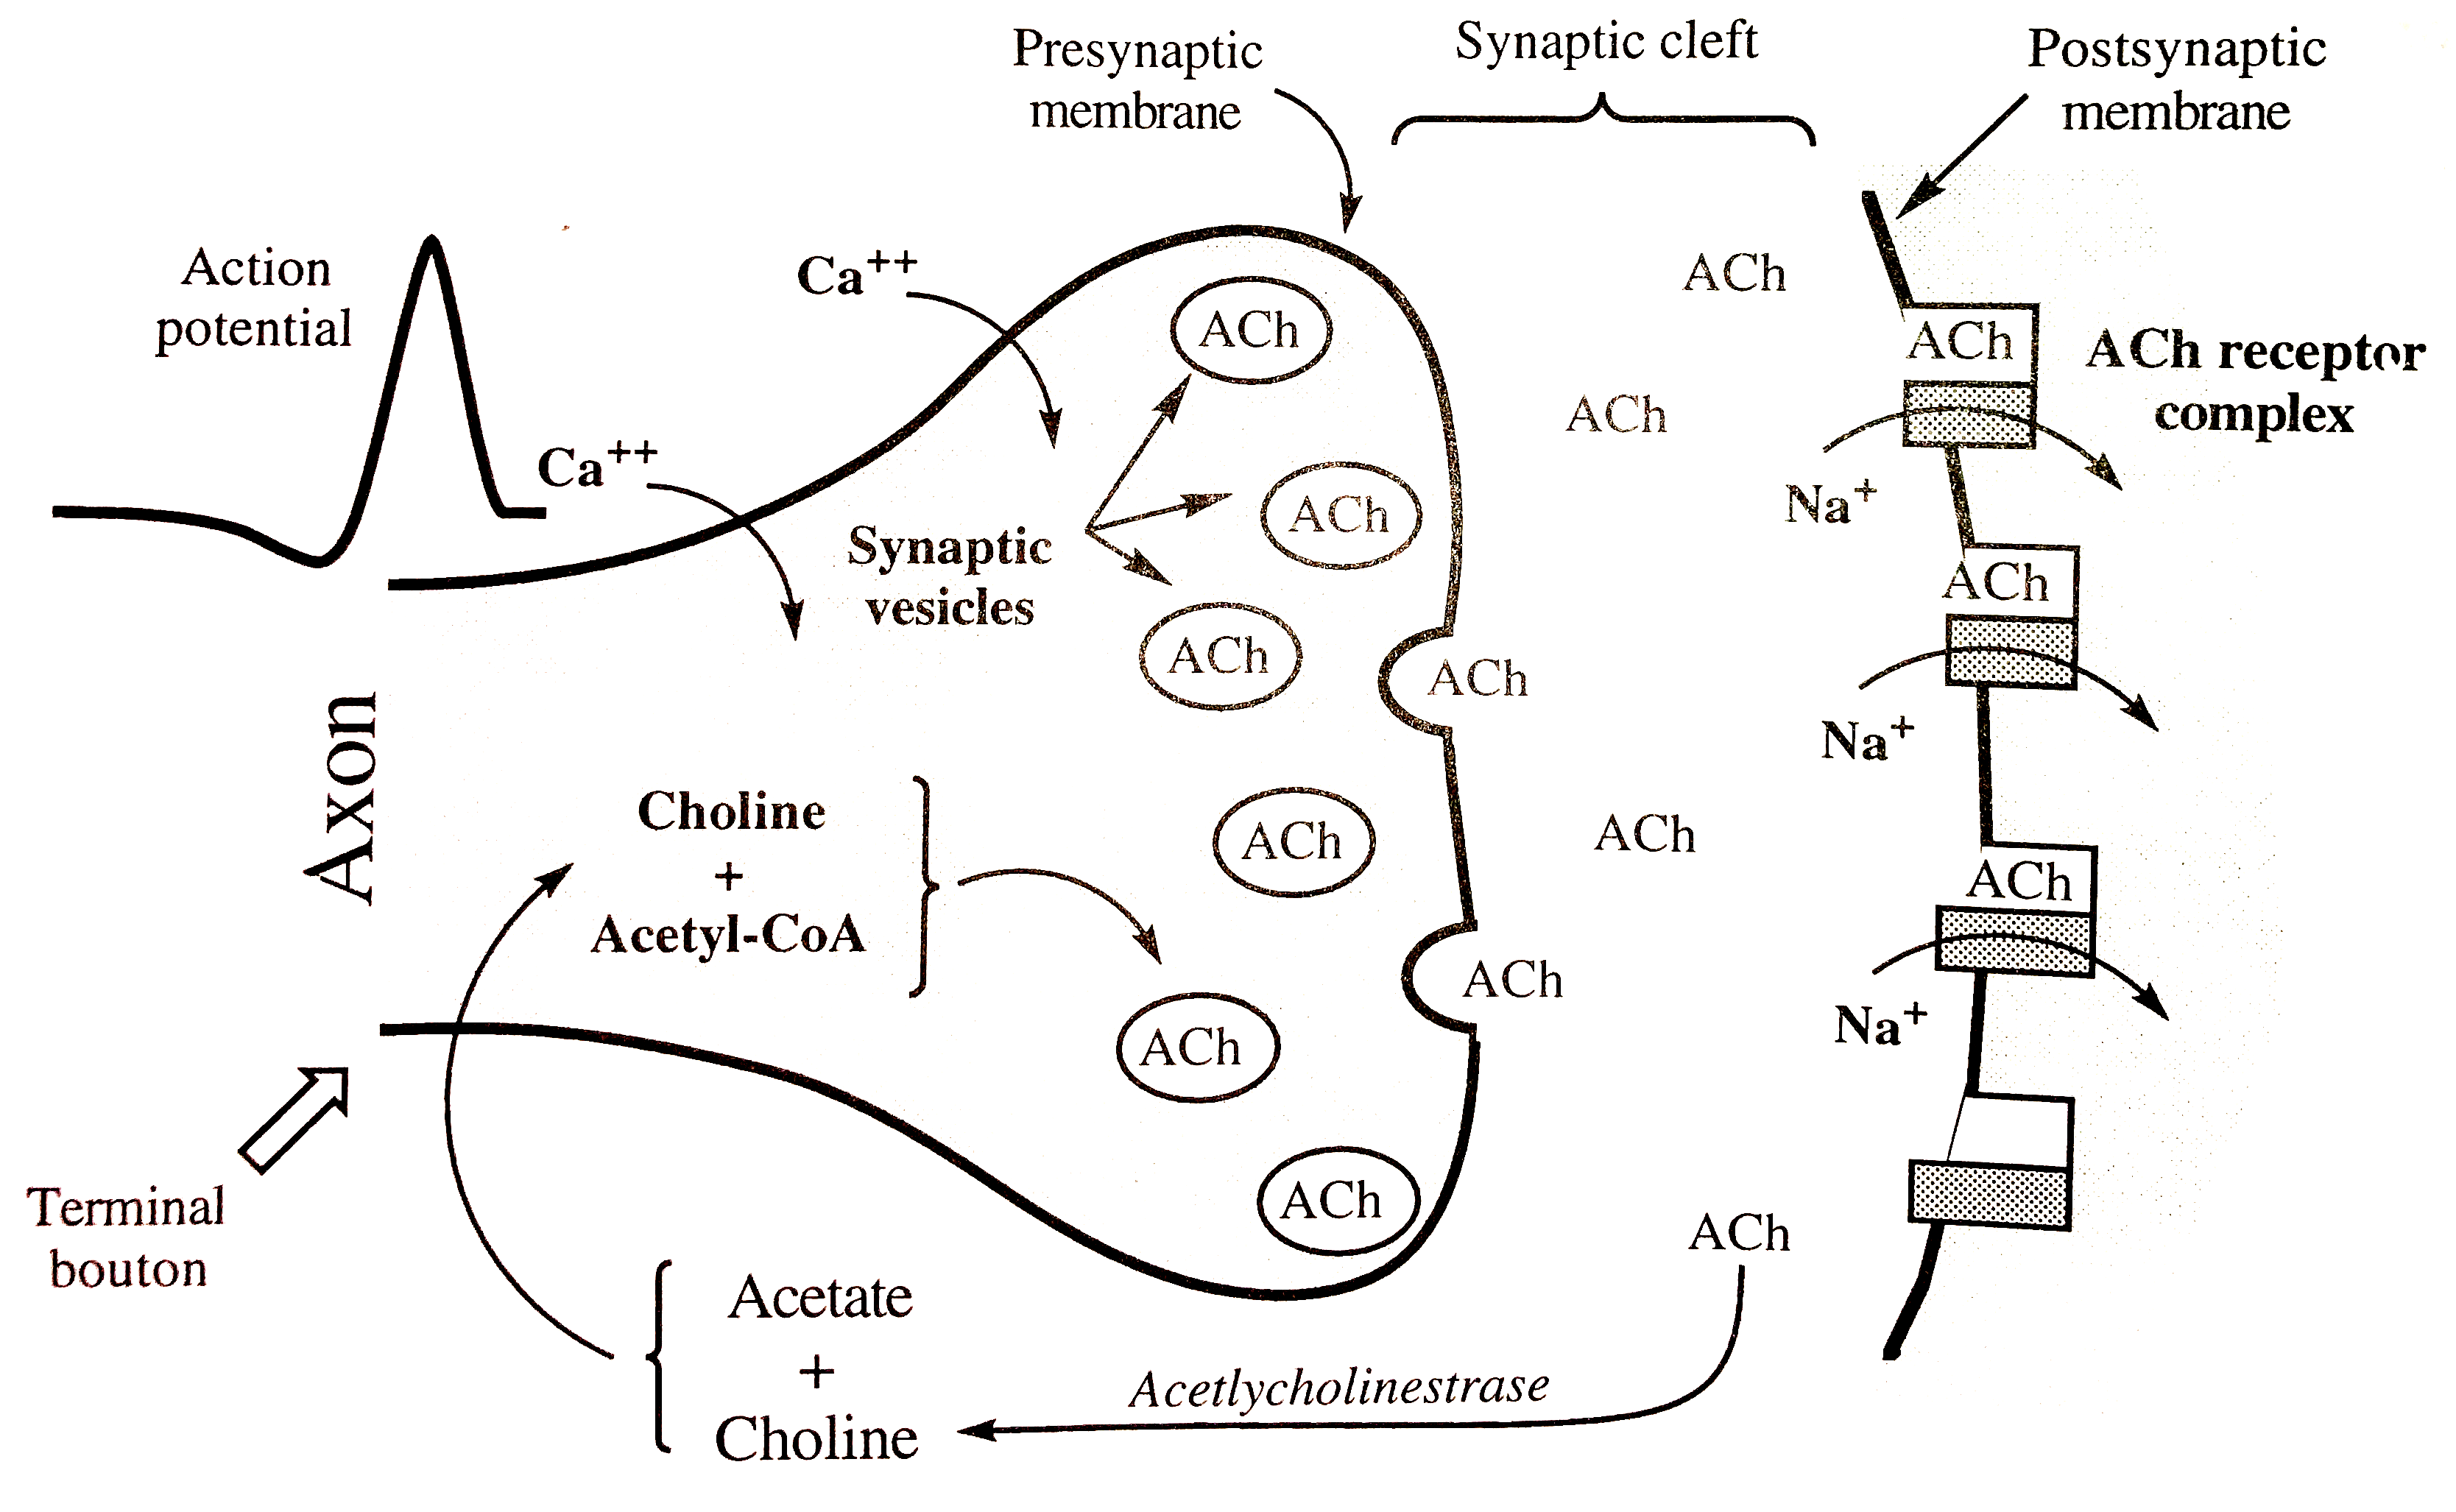
\includegraphics[width=0.7\textwidth]{neuromuscular.png} \label{neuromuscular}
\caption{Presynaptic and postsynaptic membranes of a neuromuscular junction.}
\end{figure}
\indent If ACh were to remain in the synaptic cleft, then it would continue to bind to the postsynaptic membrane and action potentials would continually be generated. This could result in prolonged muscle spasms. However, the enzyme \textbf{\textit{acetylcholinesterase}}, which is bound to the surface of the postsynaptic membrane, hydrolyzes ACh to acetate and choline. Other neurotransmitters include the amino acid \textbf{glutamate} and the amino acid derivatives \textbf{epinephrine}, \textbf{norepinephrine}, \textbf{dopamine}, and \textbf{serotonin}. \\
\indent ACh binding to its postsynaptic membrane receptor is referred to as an \textbf{excitatory} postsynaptic potential (\textbf{EPSP}s), since it elicits an excitatory response that generates an action potential. There can also be \textbf{inhibitory} postsynaptic potentials (\textbf{IPSP}s). EPSPs cause an increase in the membrane permeability to \ce{Na+} ions, while IPSPs cause an increase in the permeability of the postsynaptic membrane to \ce{K+} and \ce{Cl-} ions. \\
\indent When two action potentials are coming toward each other in the same neuron, both action potentials will be stopped when they meet. This is because the region in front of each action potential is continuously being depolarized, while the region behind the action potential is in its refractory period for a few milliseconds and cannot immediately be depolarized by the other action potential. 

\subsection{The Sarcomere} 
Muscles are multinucleated. They don't divide, but just get larger (i.e. with exercise). Skeletal muscles have \textbf{striations} in both the transverse and longitudinal directions. The striations in the longitudinal direction are due to \textbf{myofibrils}, which contain the contractile units of the muscle. Each contractile unit, bounded by a structure referred to as the \textbf{Z-line}, is referred to as a \textbf{sarcomere} and each sarcomere contains two types of contractile proteins. The thin contractile protein is called \textbf{actin} and the thick contractile protein is called \textbf{myosin}. The myosin thick filament comprises the \textbf{A-band}, and the region between two A-bands is the \textbf{I-band}. The \textbf{H-zone} is that region in the center of the A-band and between the ends of the actin filaments. All these components of the sarcomere are shown in \textbf{Fig. \ref{sarcomere}}.\\
\begin{figure}[!ht]
\centering
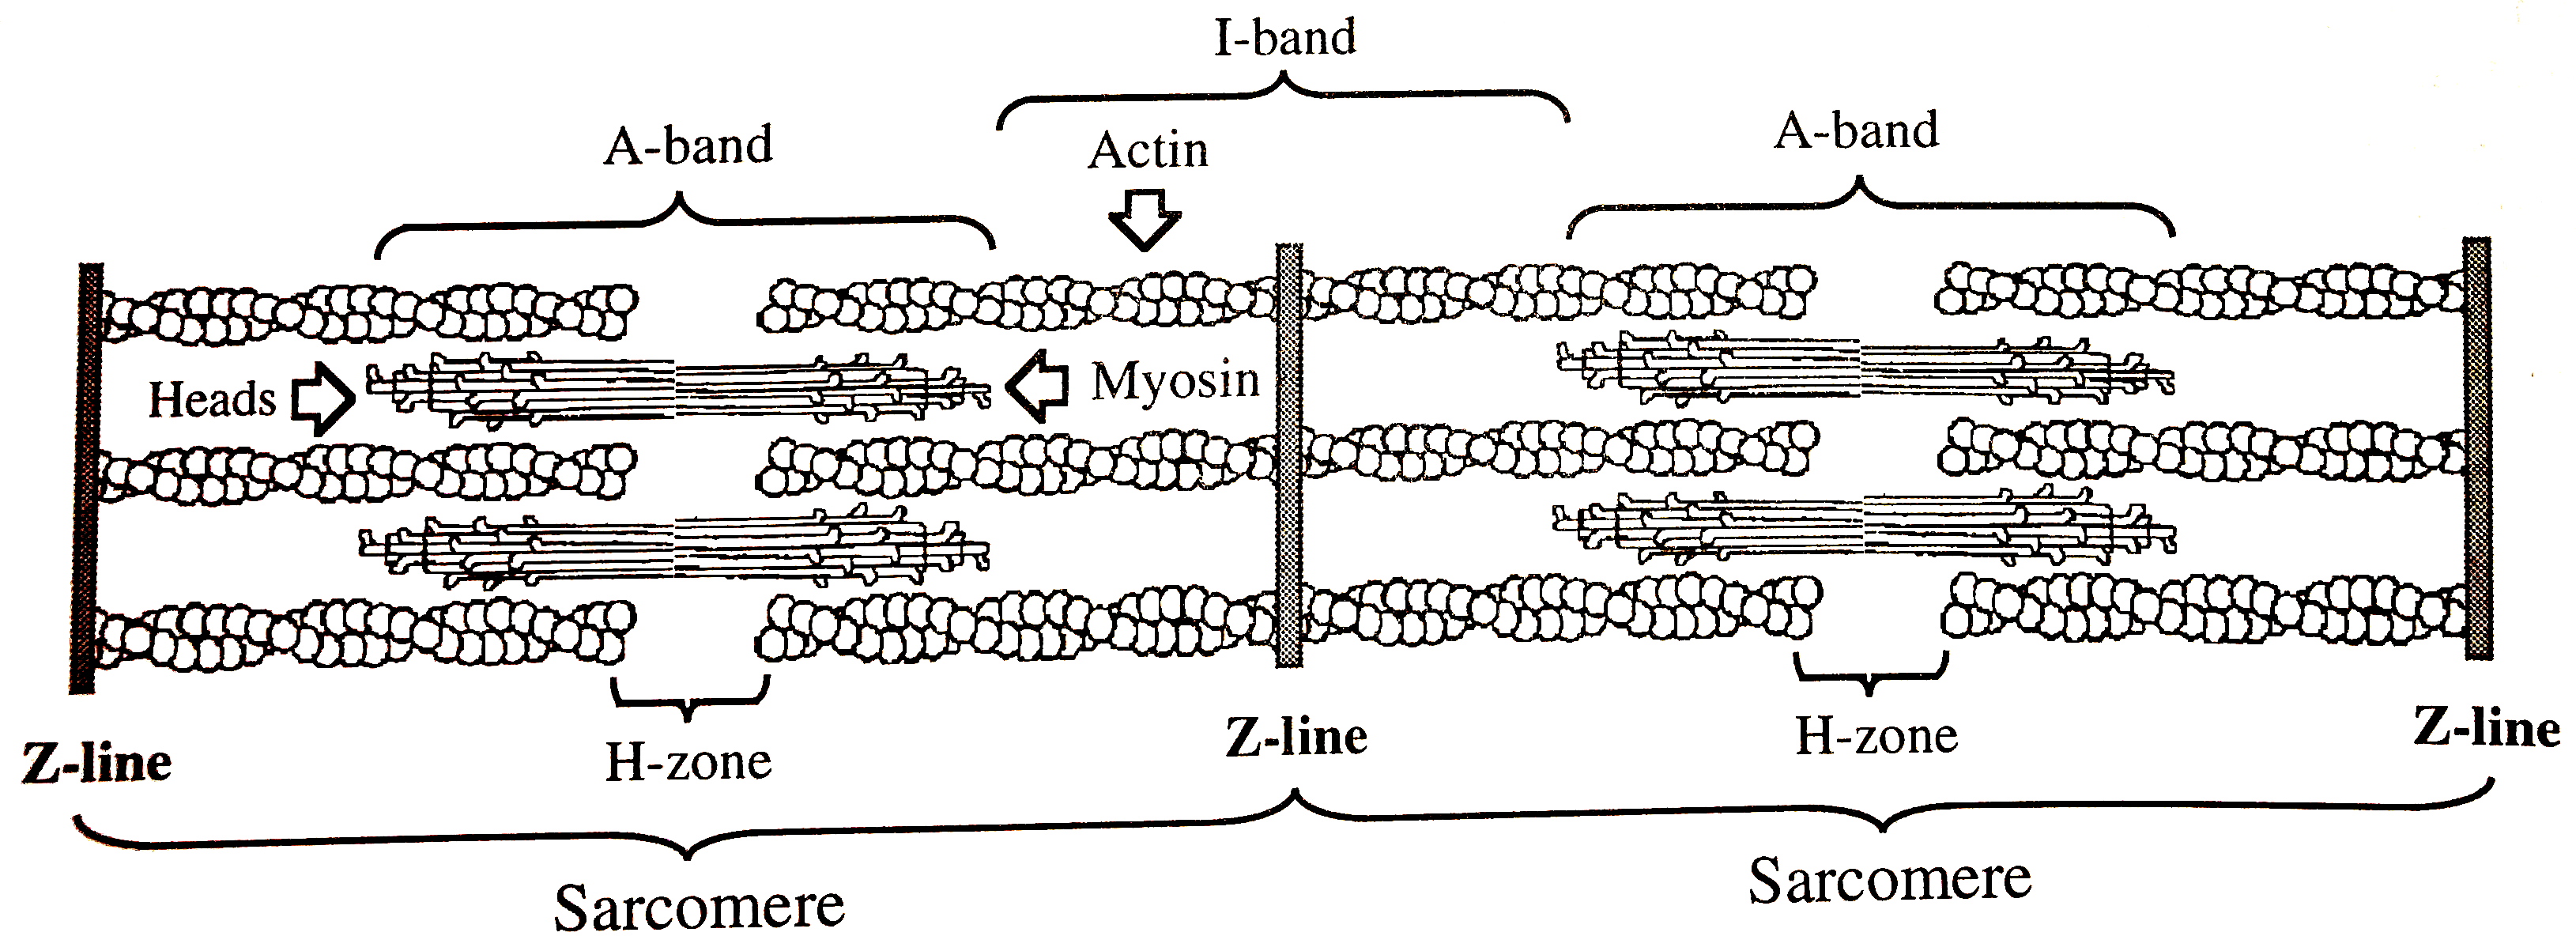
\includegraphics[width=0.7\textwidth]{sarcomere.png} \label{sarcomere}
\caption{Sarcomere details.}
\end{figure}
\indent Let's consider the interaction between actin and myosin. When a muscle is in its relaxed state, ATP is bound to the myosin head groups. The myosin head is not bound to the actin filament, because ATP reduces myosin's affinity for actin. The ATP can be hydrolyzed to ADP, and the myosin head now undergoes a corresponding conformational change that is higher in energy and stable. The myosin-ADP-\ce{P_i} (\ce{P_i} is the inorganic phosphate hydrolysis product) head complex binds to the actin filament. This step is dependent on \ce{Ca^2+} being present. The interaction between the actin filaments and myosin head groups releases the ADP and \ce{P_i} from the myosin heads, causing a conformational change in the myosin heads. This step is called the \textbf{power stroke}, and the product of this step is referred to as the \textbf{rigor complex} or \textbf{rigor state}. In order for the myosin heads to dissociate from actin filaments, ATP needs to bind to those myosin heads. This contraction cycle of muscles is shown in \textbf{Fig. \ref{contraction_cycle}}.\\
\begin{figure}[!ht]
\centering
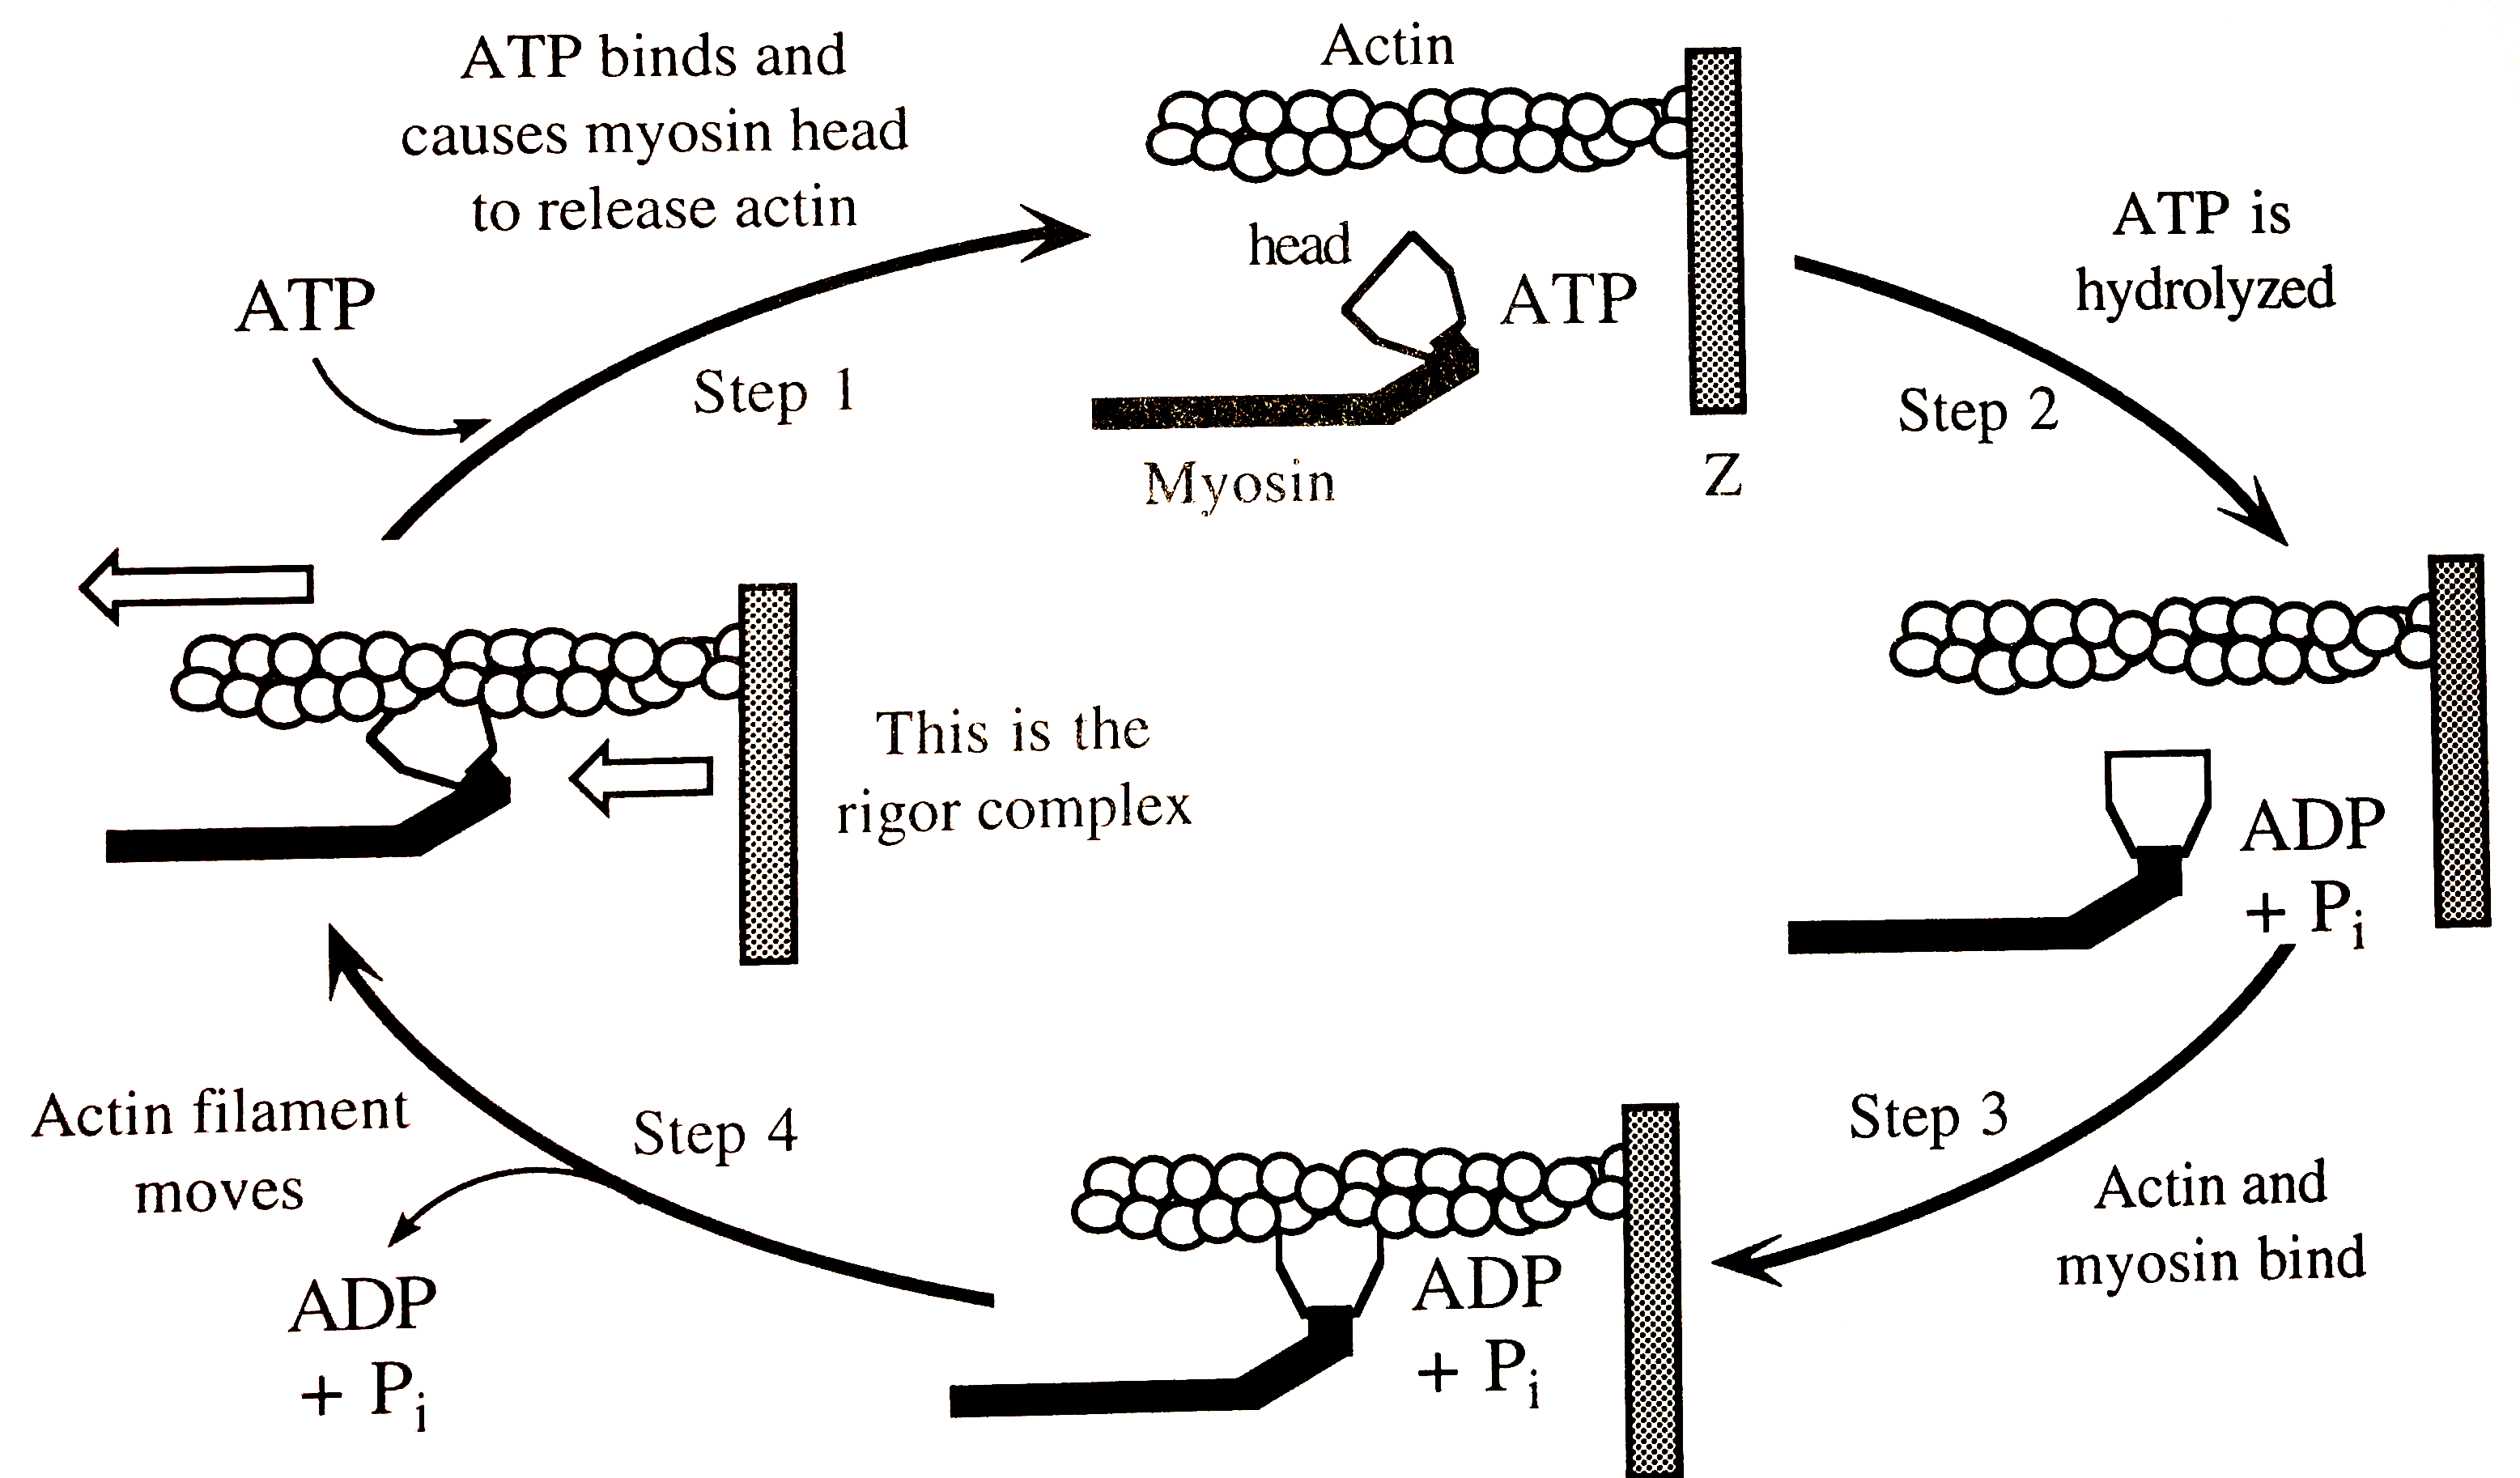
\includegraphics[width=0.7\textwidth]{contraction_cycle.png} \label{contraction_cycle}
\caption{The contraction cycle of actin and myosin.}
\end{figure}
\indent \textbf{Tropomyosin} is a protein that runs the length of the grooves of actin's helical structure. When tropomyosin resides in the actin groove, it covers up the binding sites for the myosin heads and prevents those head groups from attaching to the actin filament. \textbf{Troponin} is a binding protein that interacts with tropomyosin, actin, and \ce{Ca^2+}. When \ce{Ca^2+} is bound to a particular subunit of the troponin complex, it causes tropomyosin to shift its position and expose the myosin head binding sites. Myosin then can bind to the actin filaments, and muscle contraction follows. If \ce{Ca^2+} is not present, then no myosin binding is possible and the muscle is in the \textbf{relaxed state}. This interaction is shown in \textbf{Fig. \ref{troponin}}.\\
\begin{figure}[!ht]
\centering
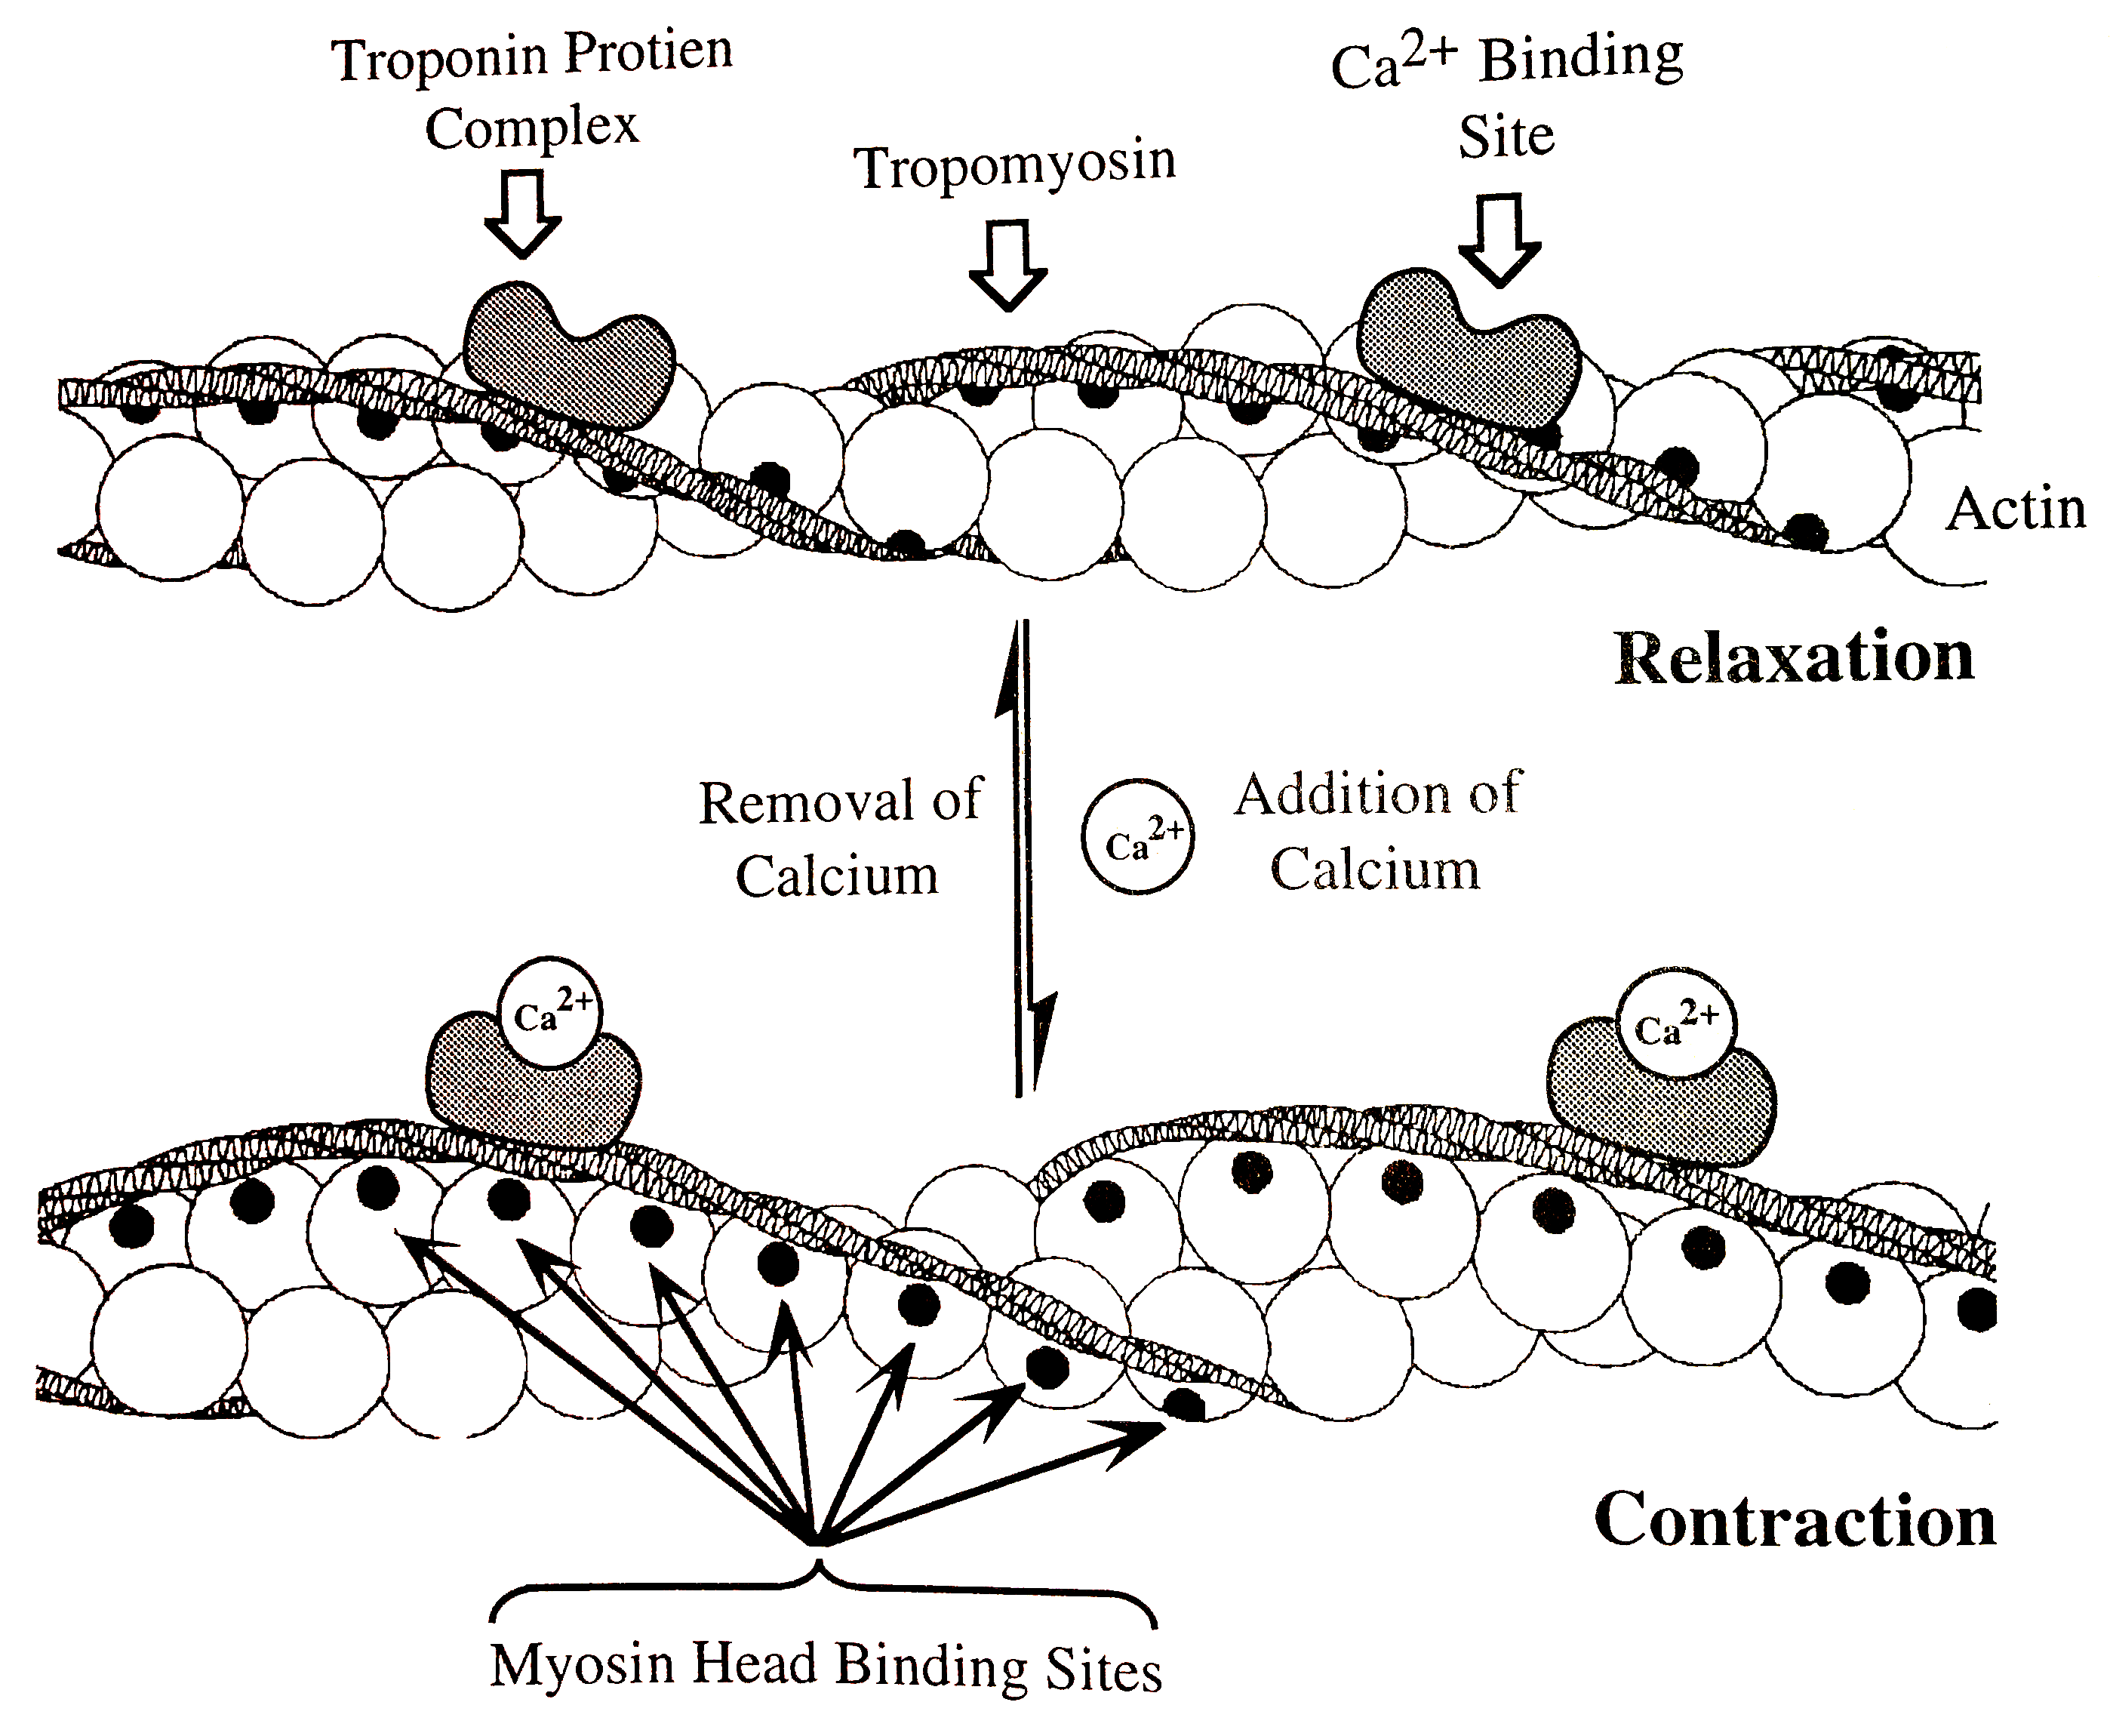
\includegraphics[width=0.7\textwidth]{troponin.png} \label{troponin}
\caption{The interaction between troponin, tropomyosin, and calcium in the sarcomere.}
\end{figure}
\indent \textbf{Myofibrils} are the basic, rod-like units of a muscle cell. Surrounding each myofibril is a membranous structure called the \textbf{sarcoplasmic reticulum}, a modified version of the endoplasmic reticulum. \ce{Ca^2+} is sequestered within this smooth membranous structure. Also surrounding each myofibril is an invagination of the sarcolemma (i.e. the plasma membrane) called the \textbf{T-tubule}. Action potentials pass down each T-tubule and stimulate the release of \ce{Ca^2+} from the sarcoplasmic reticulum. \ce{Ca^2+} then bind to the troponin complex, allowing for synchronized muscle contraction. Once contraction has taken place and the nerve impulse has ceased, the \ce{Ca^2+} in the cytosol is pumped back into the sarcoplasmic reticulum by a \ce{Ca^2+}-ATPase pump.\\
\indent The strength of muscle contraction can be varied by (1) the size of the motor unit, which is simply a motor neuron and the muscle fibers that it innervates, (2) the number of available motor units, and (3) the amount of actin and myosin contained within each cell. Smaller motor units means greater precision and lower strength. Less motor units means lower strength.
\begin{figure}[!ht]
\centering
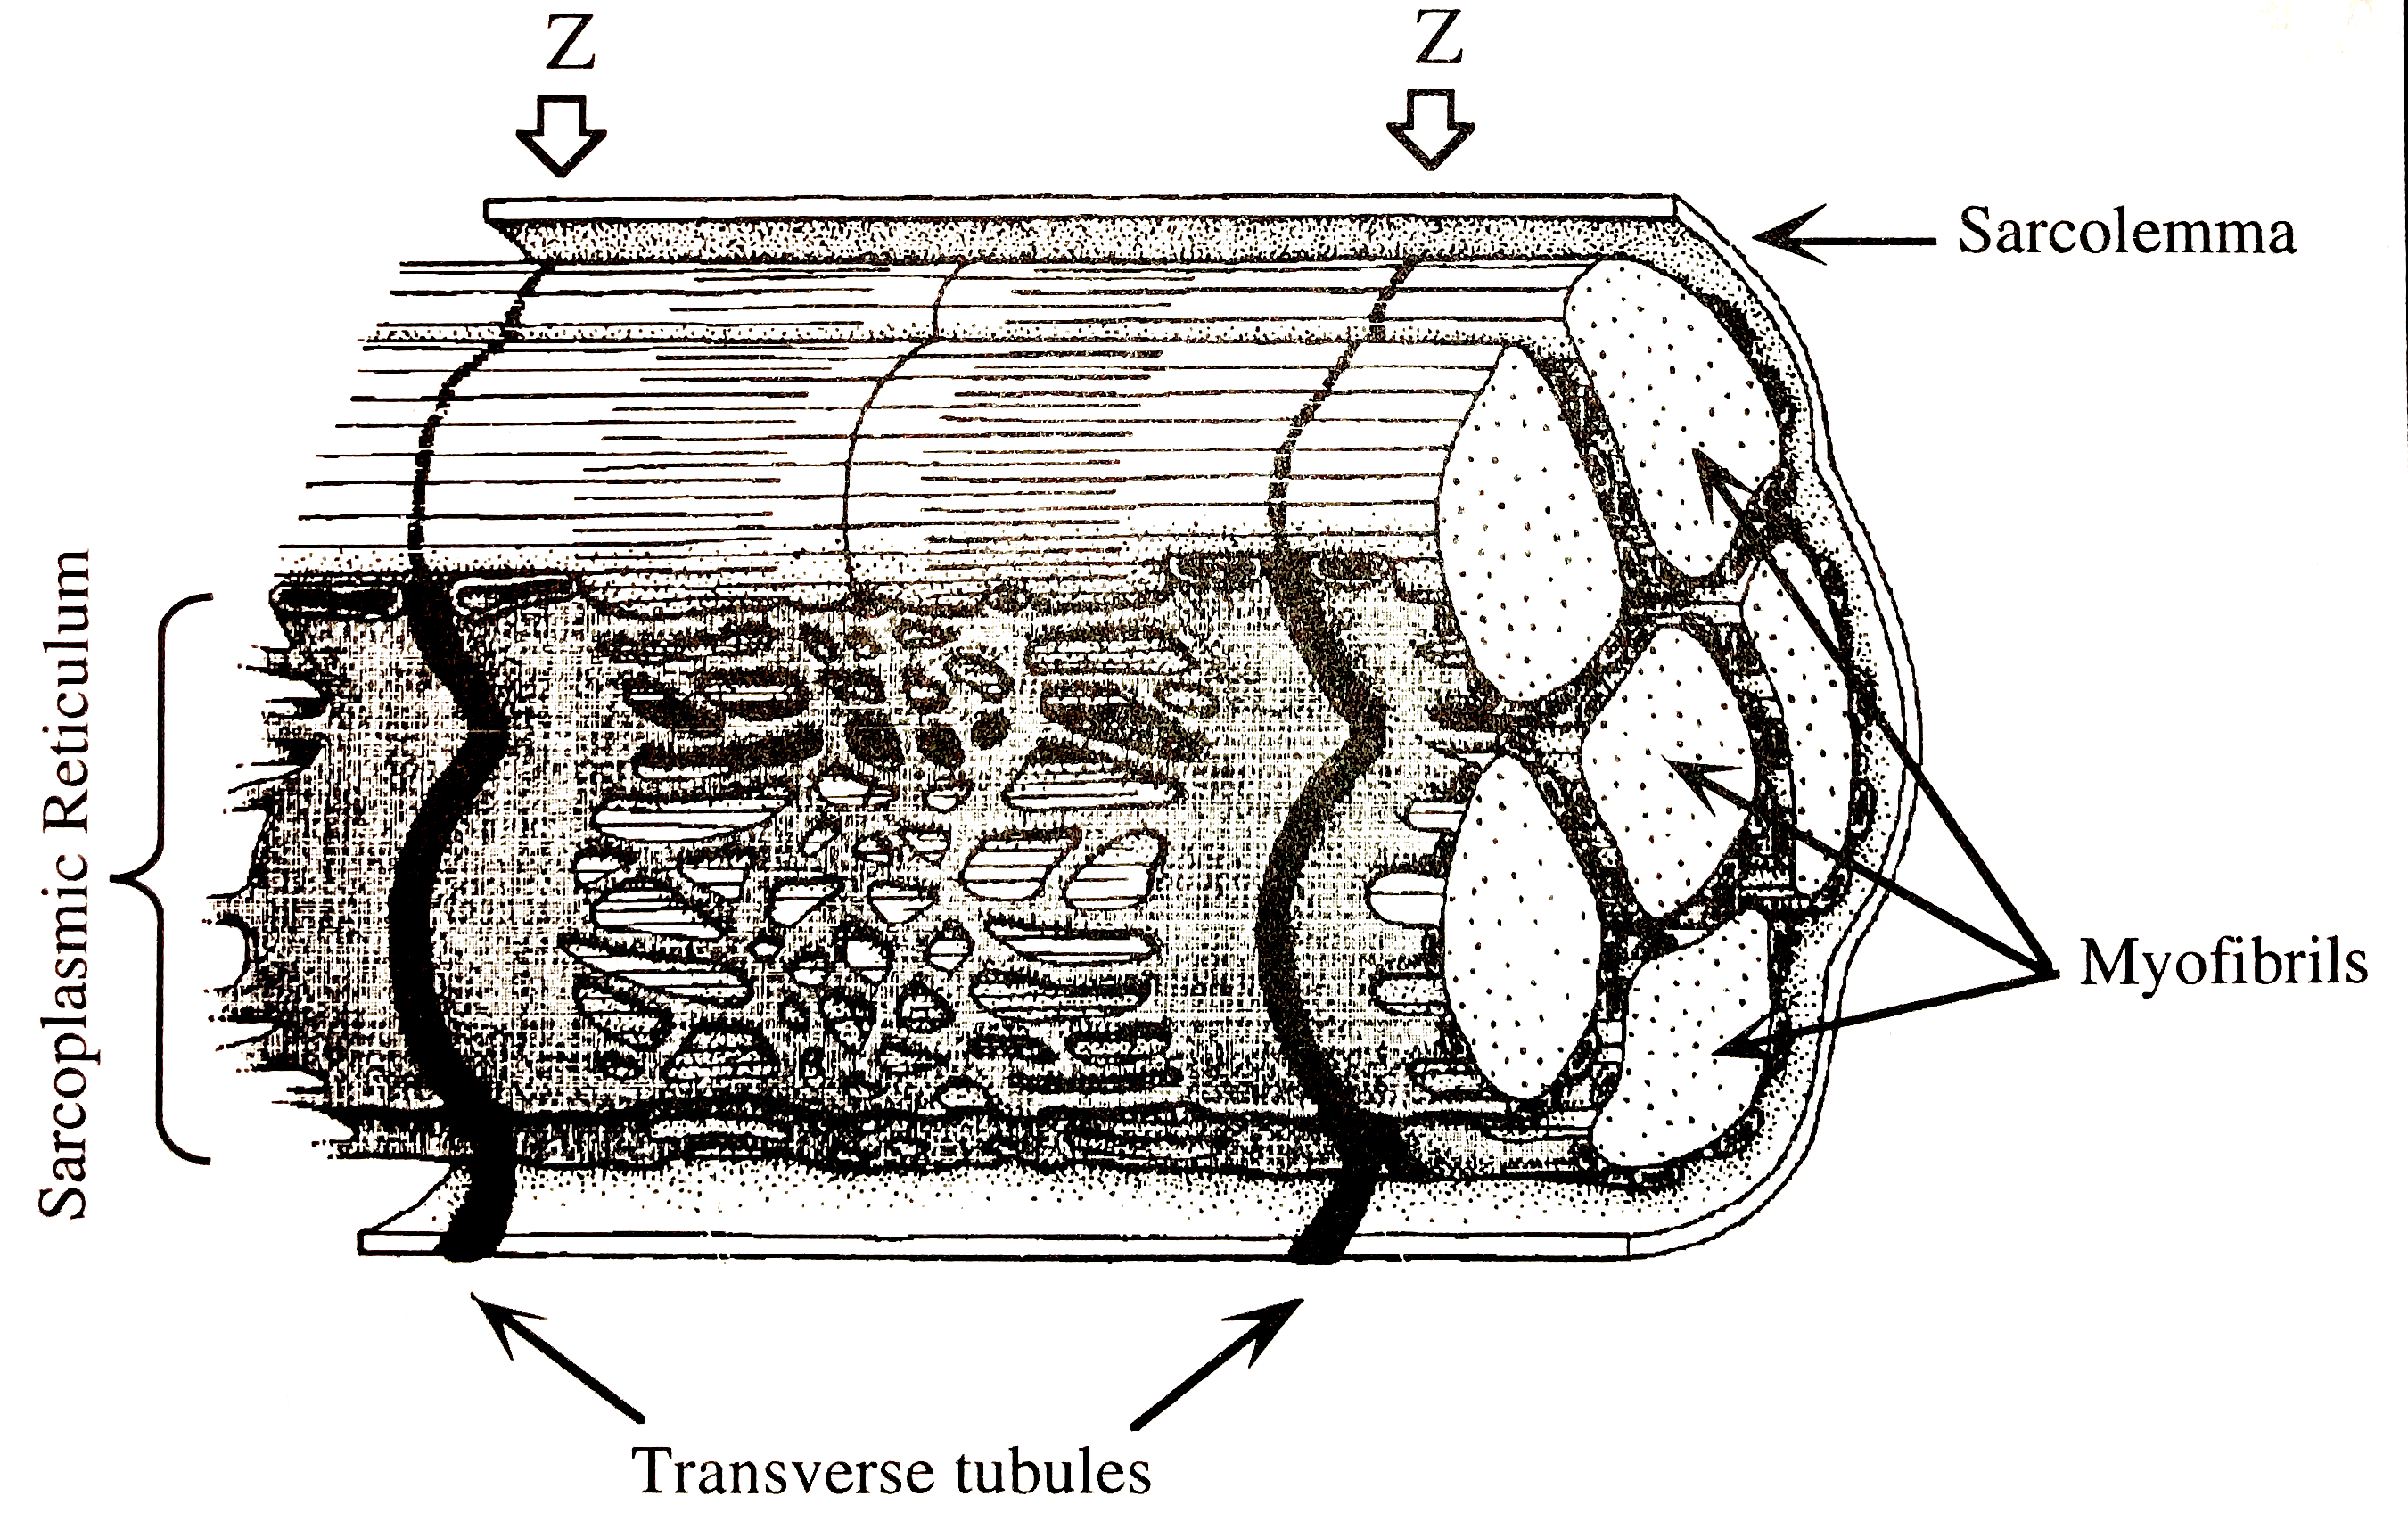
\includegraphics[width=0.7\textwidth]{sarcoplasmic_reticulum.png} \label{sarcoplasmic_reticulum}
\caption{The sarcoplasmic reticulum.}
\end{figure}

\subsection{Nervous System Components}
A grouping of nerve cells is called a \textbf{ganglion}. The three basic anatomical division of the vertebrate brain are the \textit{forebrain} (prosencephalon), \textit{midbrain} (mesencephalon), and \textit{hindbrain} (rhombencephalon). Inferior to the brain is the spinal cord, from which the nerves extend into the limbs and extremities. If a neuron carries information \textit{into} the spinal cord and brain, that neuron is said to be an \textbf{afferent (sensory) neuron}. If a neuron carries the information away from the CNS, that neuron is said to be an \textbf{efferent (motor) neuron}. \\
\indent The \textbf{prosencephalon} includes the \textbf{cerebrum}, \textbf{thalamus}, and \textbf{hypothalamus}. The cerebrum is divided into the right and left cerebral hemispheres, joined by the \textbf{corpus callosum}. The cerebral hemispheres are divided into the \textbf{frontal lobes} (associated with movement and personality), \textbf{parietal lobes} (associated with touch and stretch sensation), \textbf{occipital lobes} (associated with vision), and \textbf{temporal lobes} (associated with hearing). The outermost layer of the cerebrum is called the \textbf{cerebral cortex}, consisting of \textbf{gray matter} (nerve cell bodies and their dendrites) and \textbf{white matter} (myelinated axons of the nerve cells). In the spinal cord, the gray matter is more centralized, while the white matter is more peripheral. The anatomical divisions of the vertebrate brain are shown in \textbf{Fig. \ref{brain}}.\\
\begin{figure}[!ht]
\centering
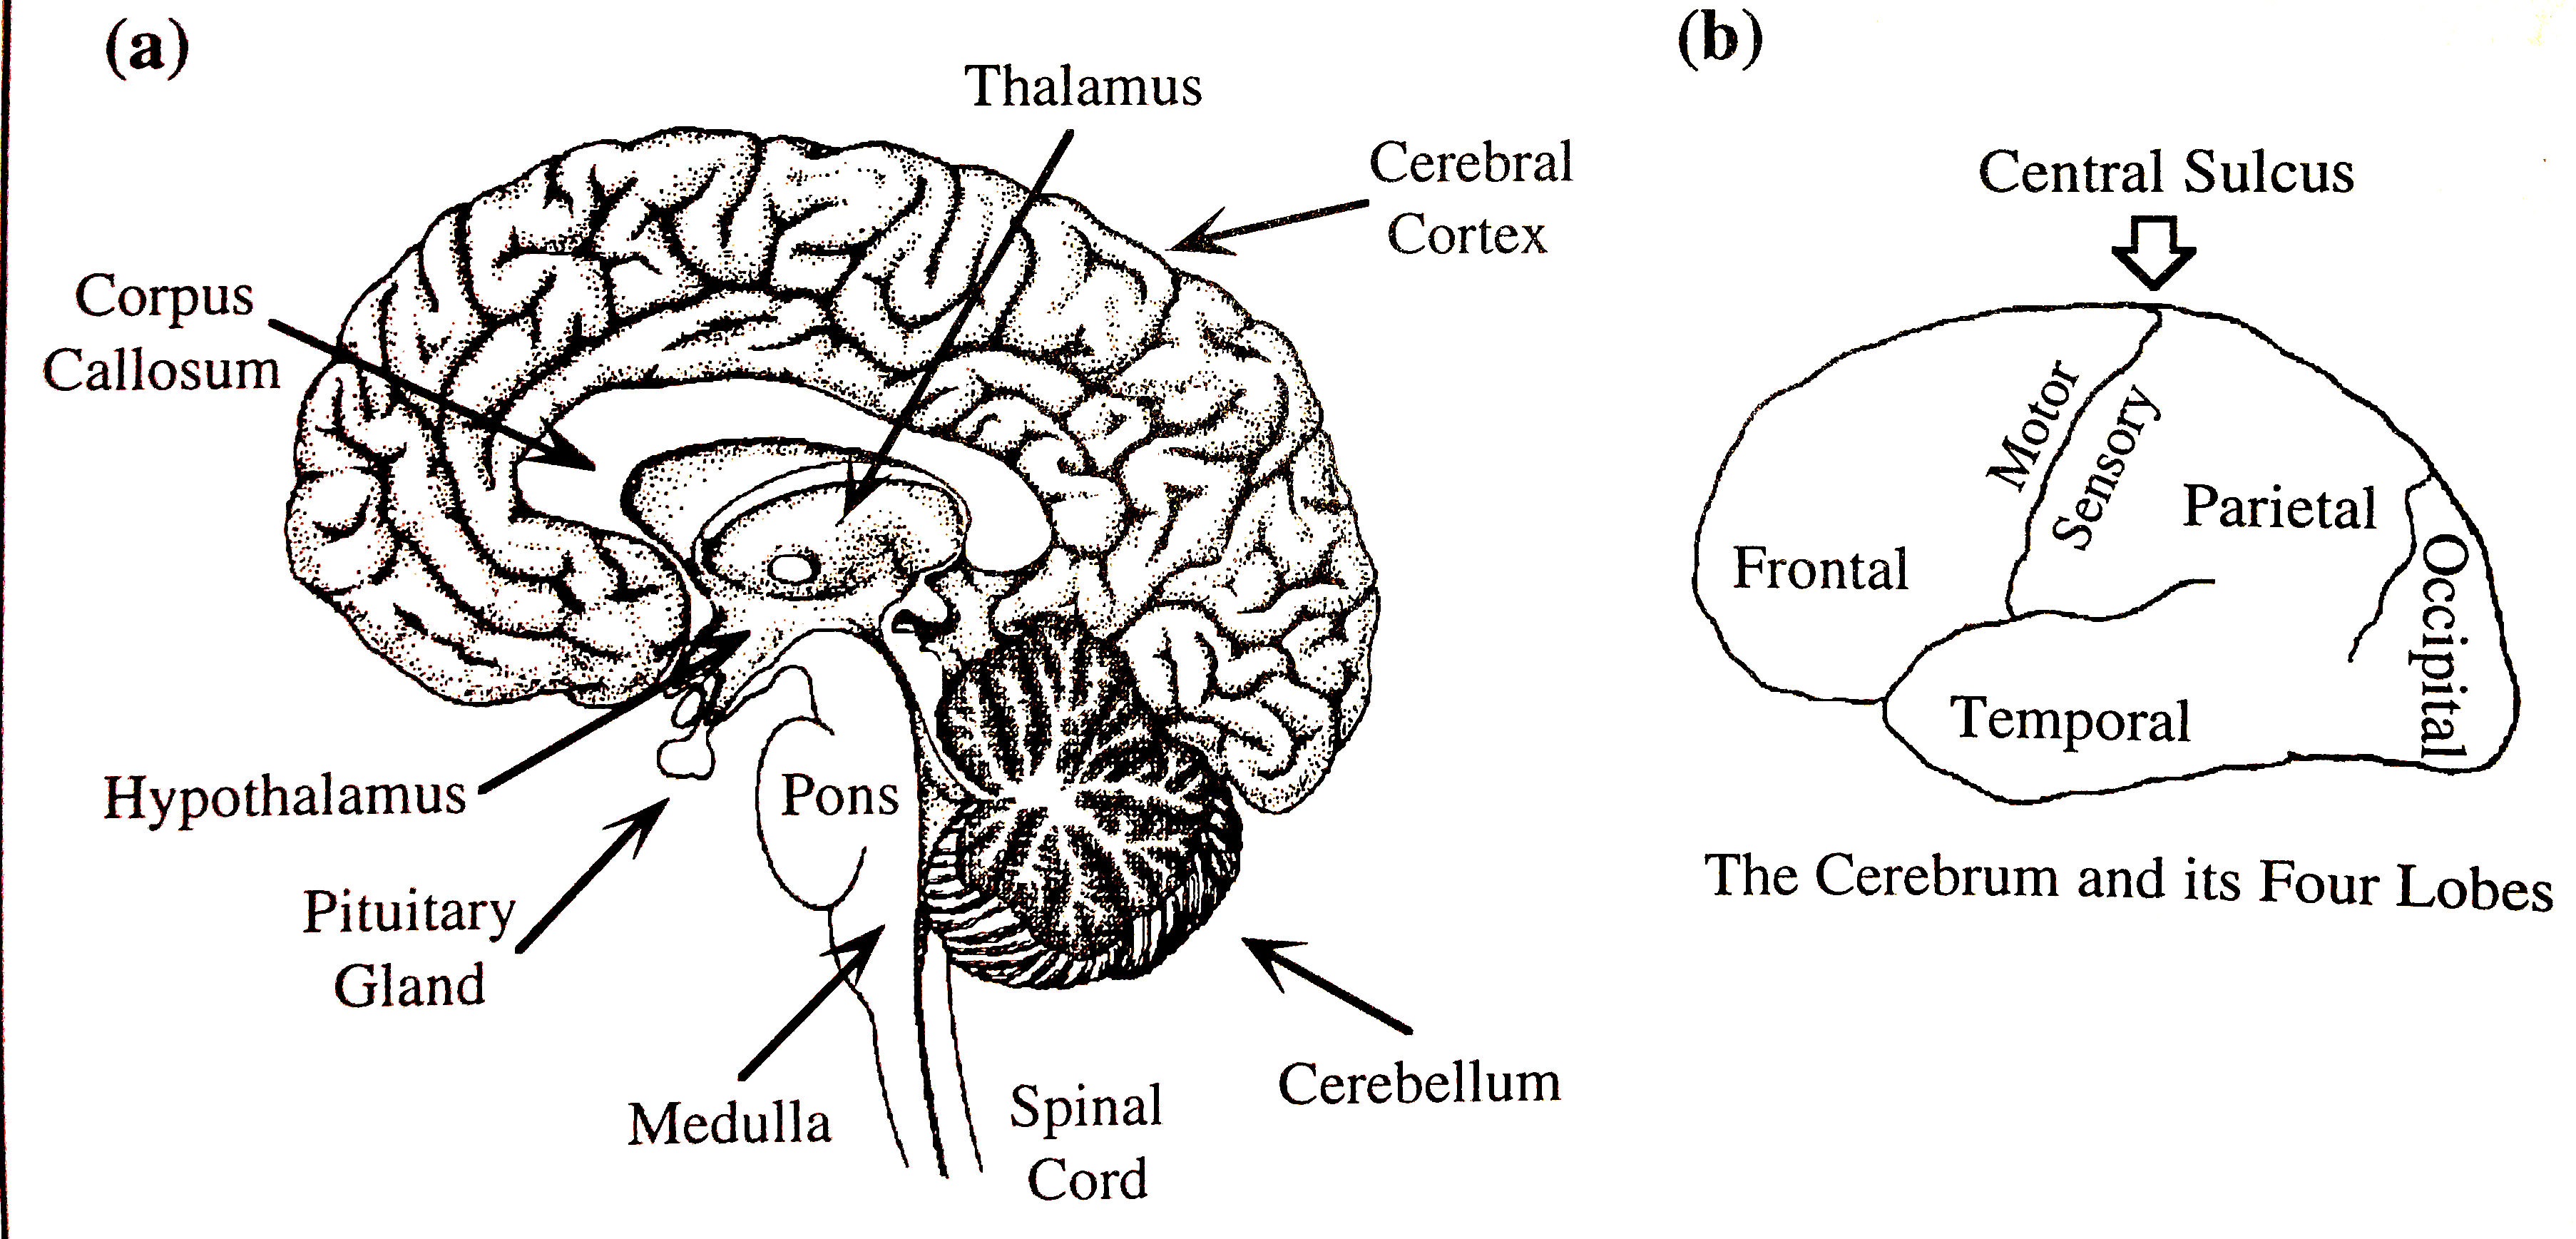
\includegraphics[width=0.7\textwidth]{brain.png} \label{brain}
\caption{Anatomical divisions of the vertebrate brain.}
\end{figure}
\indent The \textbf{central sulcus} is a prominent groove that separates the frontal lobes and parietal lobes. Anterior to the sulcus is the \textbf{motor cortex}, which controls the movement of individual muscles. Posterior to this sulcus is the \textbf{sensory cortex}, which detects sensations in various parts of the body. \\
\indent The \textbf{thalamus} is a relay station for much of the visual and auditory information from the environment. The \textbf{hypothalamus} is concerned with the visceral (subconscious) activities of the body. The \textbf{pituitary gland} is the master endocrine gland of the body\textemdash it receives information from the hypothalamus and sends out information to regulate different parts of the body. \\
\indent The \textbf{brainstem} contains the \textbf{midbrain}, \textbf{cerebellum}, \textbf{pons}, \textbf{medulla}, and the \textbf{reticular formation}, which in general coordinate motor and visceral activities. The midbrain detects movement and can direct the head and eyes towards that movement. It can also sense pleasure and pain. The cerebellum is responsible for the bulk of regulation and coordination of muscular activity. The pons and medulla coordinate visceral activities. The reticular formation, which is the core of the brainstem, is essentially an activating system designed to alert the brain. It also inhibits motor and sensory impulses and can induce sleep. Below the medulla is the spinal cord. 

\subsection{Control of Body Activity and the Neurovisceral Control}
A response that makes just one synaptic connection is referred to as a \textbf{monosynaptic reflex arc}, while a response that makes at least two synaptic connections is referred to as a \textbf{polysynaptic reflex arc}. \\
\indent The \textbf{autonomic} nervous system is part of the \textbf{efferent} division of the PNS, which can be further subdivided into the \textbf{sympathetic} and the \textbf{parasympathetic} systems. The \textbf{parasympathetic division} of the autonomic nervous system has nerve fibers which leave from the \textbf{sacral} portion of the spinal cord and from the midbrain (mesencephalon) and medulla (part of the rhombencephalon). Parasympathetic nerve impulses tend to increase the rate of digestion and lower the heart rate. The blood pressure is also lowered, and the pupils constrict. In general, the parasympathetic division conserves energy and helps in the restoration of various bodily functions. The parasympathetic division has both \textbf{preganglionic} and \textbf{postganglionic} nerve fibers. The cell bodies of the preganglionic neurons are found in the sacral region of the spinal cord and in the brainstem. The preganglionic nerve fibers are rather long, while the postganglionic nerve fibers are rather short. Both the preganglionic and the postganglionic nerve fibers in the parasympathetic division release ACh as the neurotransmitter. (Nerve fibers that release ACh as their neurotransmitter are called \textbf{cholinergic} nerve fibers. \\
\indent The most prominent nerve in the parasympathetic division is the \textbf{vagus nerve}, which innervates the heart, lungs, stomach, liver, small intestine, large intestine, and kidneys, among other organs. An overview of the parasympathetic nervous system is shown in \textbf{Fig. \ref{parasympathetic}}.\\
\begin{figure}[!ht]
\centering
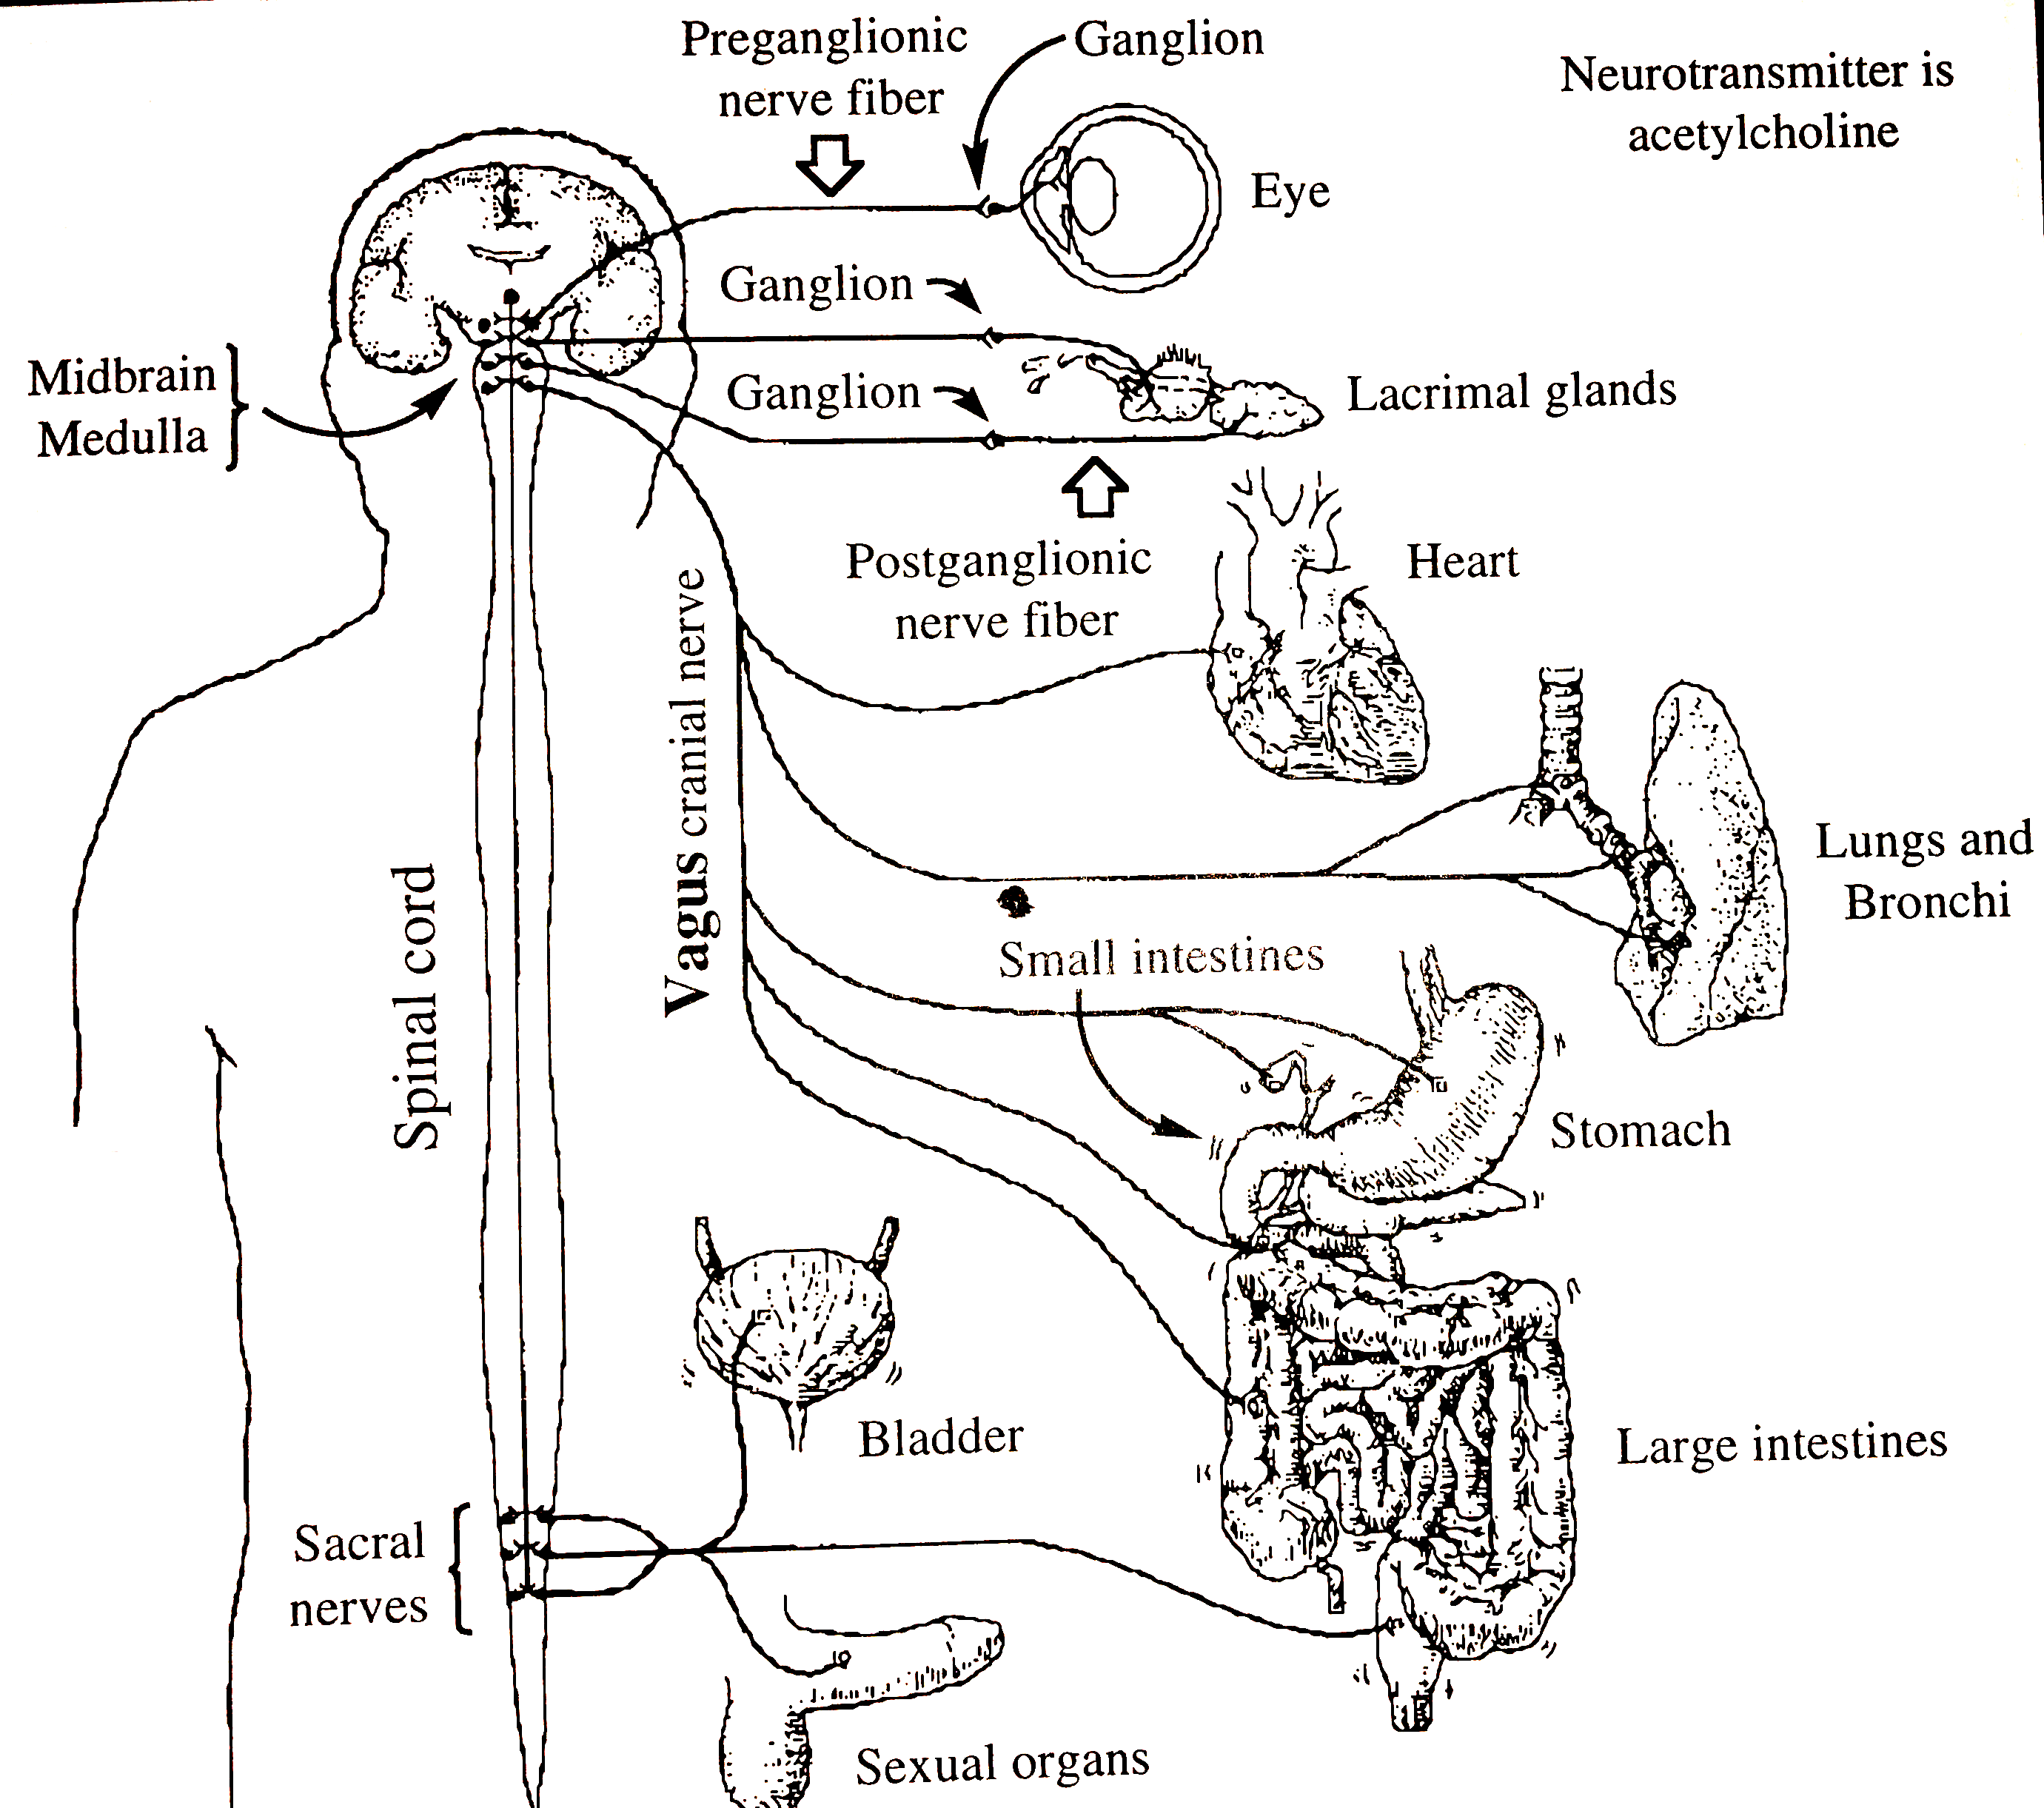
\includegraphics[width=0.7\textwidth]{parasympathetic.png} \label{parasympathetic}
\caption{Parasympathetic nerves and the parasympathetic division of the automatic nervous system.}
\end{figure}
\indent The sympathetic division of the autonomic nervous system has nerve fibers branching off from the \textbf{thoracic} and \textbf{lumbar} regions of the spinal cord. Sympathetic nerve fibers tend to condition the body for a `fight-or-flight' response. The heart rate increases, blood pressure elevates, pupils dilate, and the digestive functions decrease, all as a result of sympathetic nervous innervation. The nerve fibers leaving a synapse in a given ganglion are referred to as \textbf{postganglionic} nerve fibers. In the case of the sympathetic division the preganglionic nerve fibers tend to be short, while the postganglionic nerve fibers tend to be longer. The preganglionic fibers release ACh, while the postganglionic fibers release norepinephrine as their neurotransmitters.\\
\indent An important set of spinal nerves in the sympathetic division are the long preganglionic nerve fibers to the \textbf{adrenal medulla}. There are no postganglionic nerve fibers here\textemdash when the adrenal medulla is stimulated, both \textbf{norepinephrine} and \textbf{epinephrine} are released directly into the bloodstream. \\
\indent The \textbf{somatic} nervous system has some notable characteristics:
\begin{enumerate}
	\item Once the nerve fibers leave the CNS, they do not make a synapse until they have reached their effector organ.
	\item When the synapse is made at the effector organ, the neurotransmitter that is released is \textbf{acetylcholine}.
	\item The somatic nervous system innervates skeletal muscle. 
	\item Innervation of that skeletal muscle leads to excitation of the muscle itself. 
\end{enumerate}
\indent In contrast, the \textbf{autonomic} nervous system has some notable characteristics:
\begin{enumerate}
	\item Once the nerve fibers leave the CNS, they synapse with a ganglion before they make the final synapse with their effector organ.
	\item The preganglionic fibers in both the parasympathetic and sympathetic divisions released acetylcholine as the neurotransmitter. The postganglionic fibers in the parasympathetic division release acetylcholine; in the sympathetic division, norepinephrine is released.
	\item The autonomic nervous system innervates glands, and smooth and cardiac muscle. 
	\item The cells innervated by the autonomic nervous system can be either excitatory or inhibitory. 
\end{enumerate}
\indent The \textbf{adrenal medulla}, a specialized ganglion in the sympathetic division of the autonomic nervous system, is directly stimulated by a preganglionic fiber. This nerve fiber releases ACh, which causes the cells of the adrenal medulla to release epinephrine primarily and also norepinephrine. A review of the CNS and PNS is shown in \textbf{Fig. \ref{CNSPNS}}.
\begin{figure}[!ht]
\centering
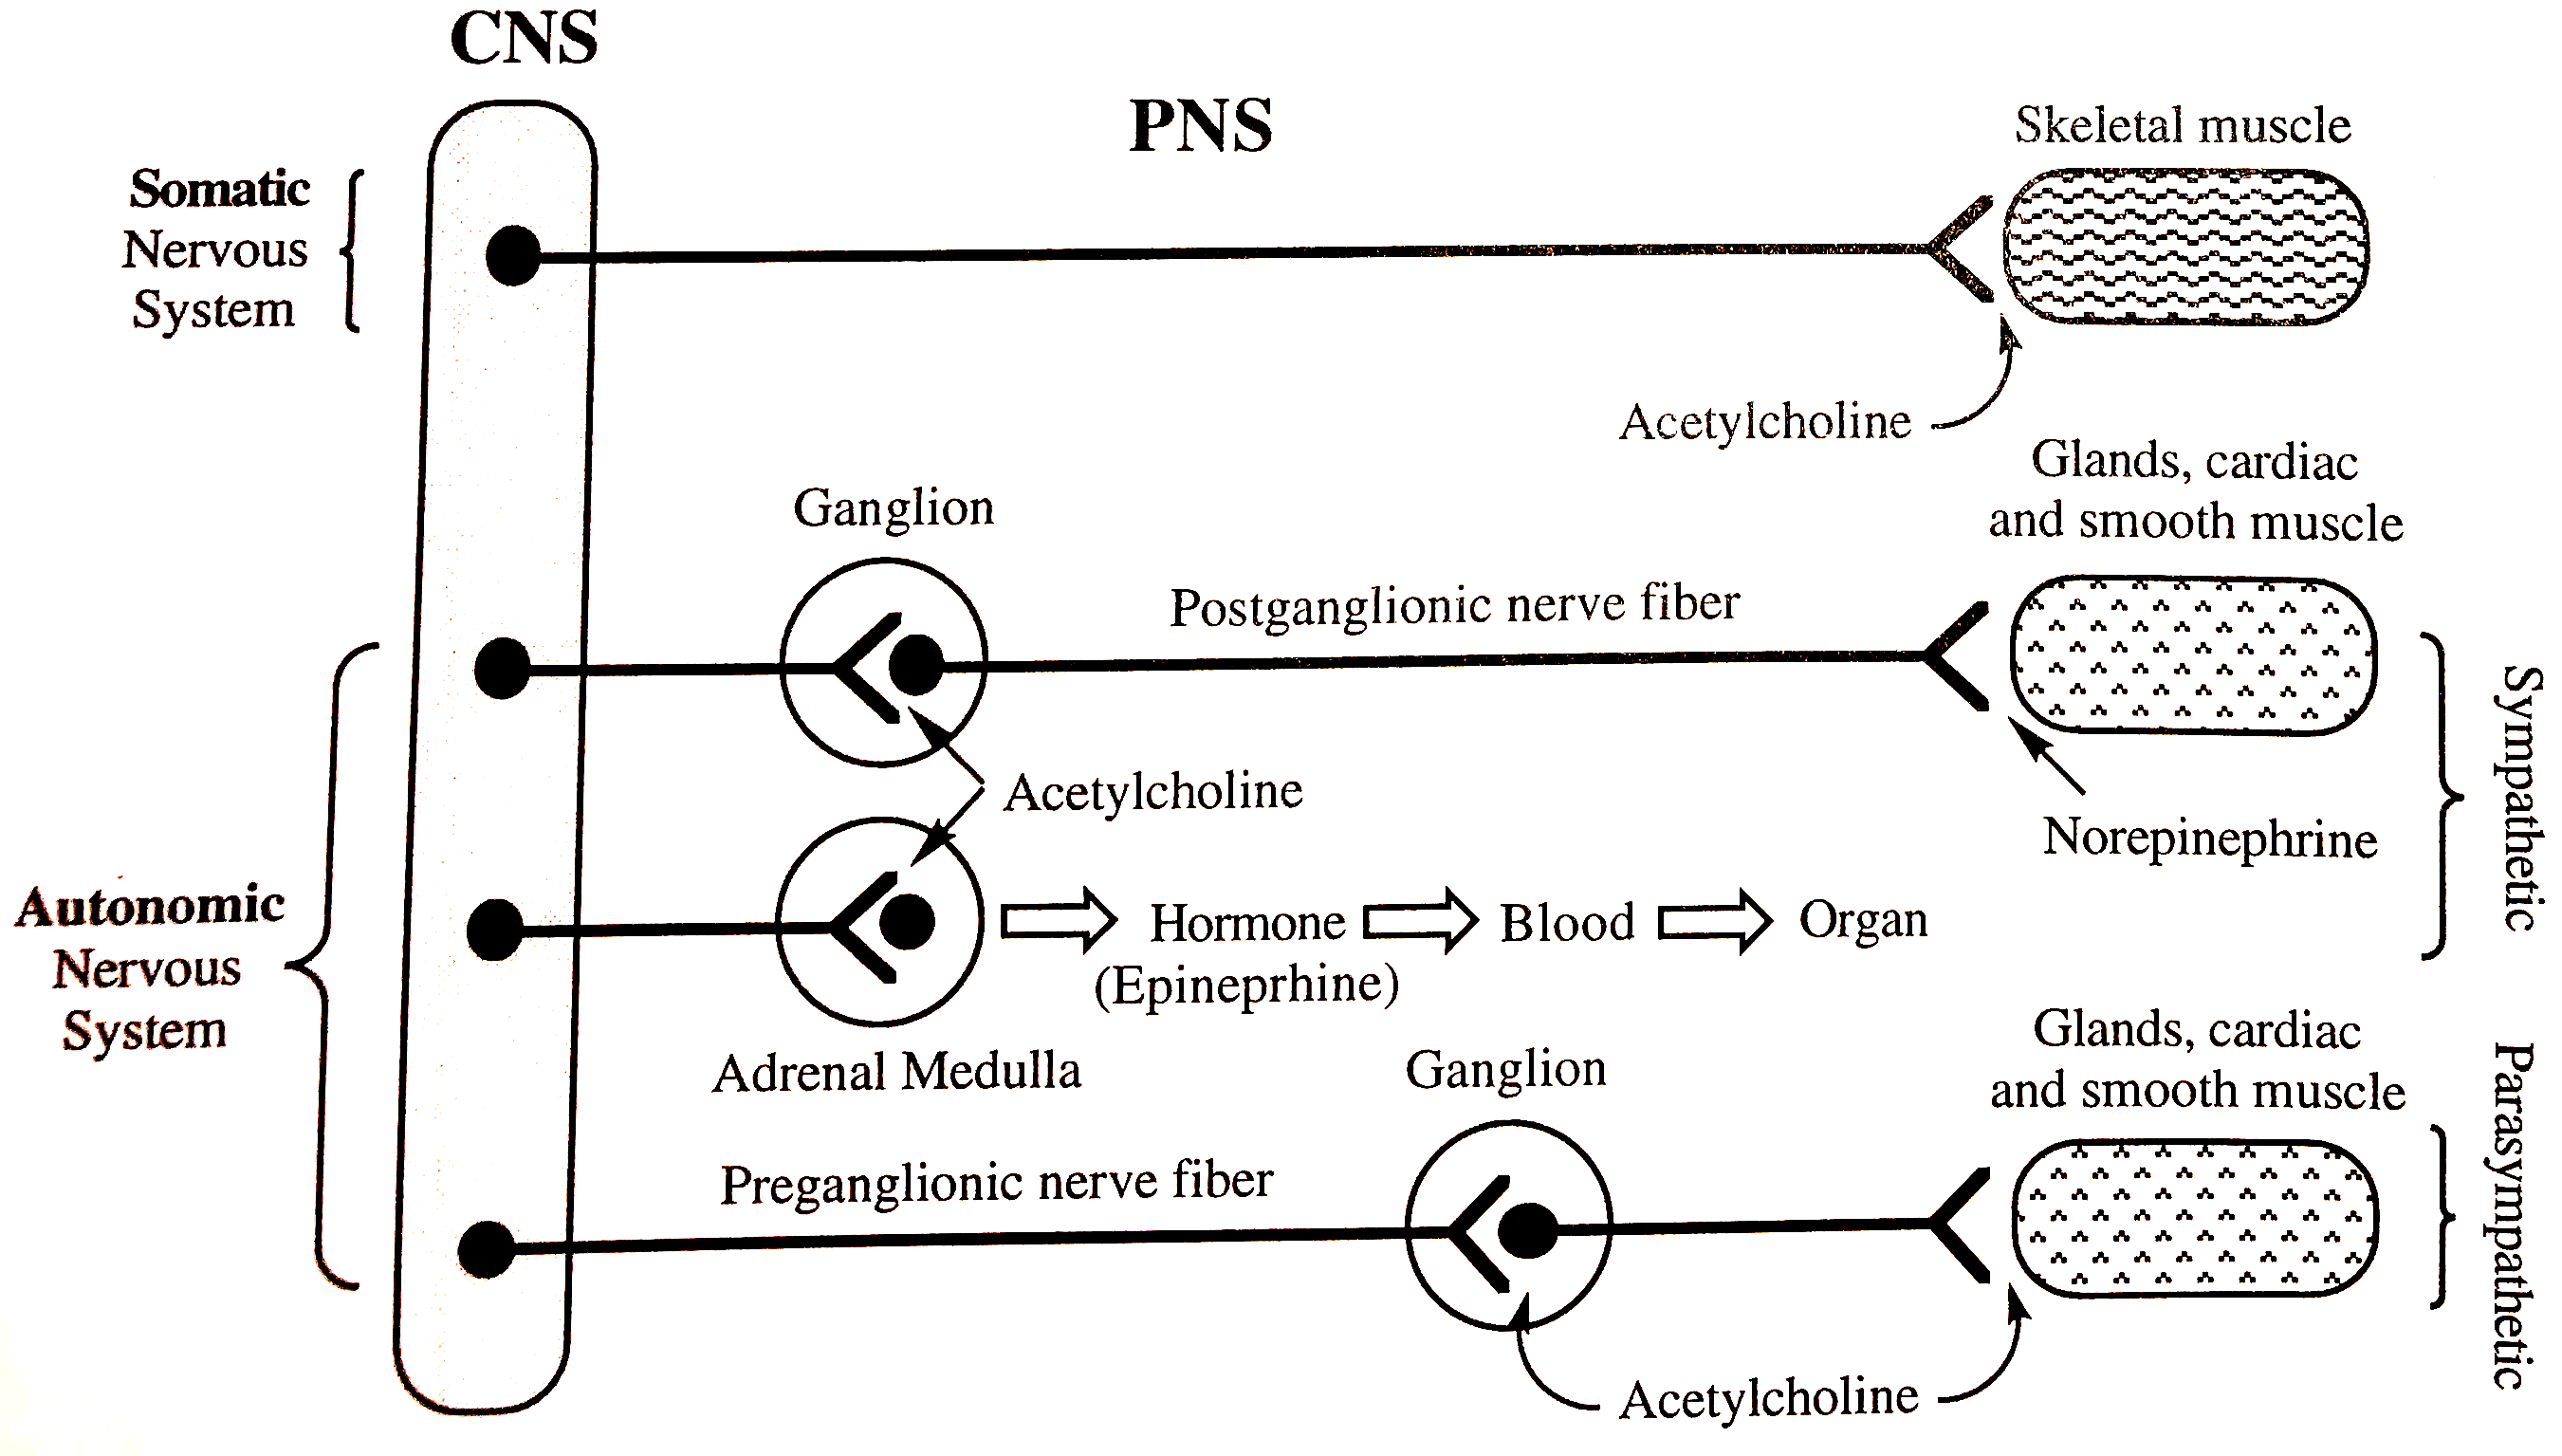
\includegraphics[width=0.7\textwidth]{CNSPNS.png} \label{CNSPNS}
\caption{CNS and PNS review.}
\end{figure}

\subsection{Receptors and Sensory Input}
\textbf{Nocirceptors} sense pain. In general, the things that are important in propagating signals in the nervous system are the frequency of action potentials, not the magnitude, as the magnitude of action potentials is always basically the same. All receptors essentially function on this basic principle. \textbf{Sensory adaptation} is the phenomenon where the body doesn't keep responding to repeated stimuli. 

\subsection{Cardiovascular Anatomy}
The function of the \textbf{circulatory system} is to bring nutrients and oxygen to the tissues of the body while simultaneously removing waste products from those same tissues. Because the circulatory system is continually flowing, it also helps to maintain body temperature. Also, the circulatory system can act as a means to transport hormones to various locations within the body. The blood that is pumped from the right heart to the lungs and back to the left heart is called the \textbf{pulmonary circulation} while the blood that is pumped from the left heart to the rest of the tissues and back to the right heart is called the \textbf{systemic circulation}. Both these circulations lie in series with right another.\\
\indent Deoxygenated blood passes from the right atrium into the right ventricle, and then is pumped to the \textbf{pulmonary artery} and to the lungs where it is oxygenated. The oxygenated blood then returns to the left heart by the \textbf{pulmonary veins}. The blood enters the left atrium and passes into the left ventricle where it is pumped out the \textbf{aorta} and to the branching arteries, arterioles, and capillaries. It is at the level of the capillaries that the blood exchanges nutrients and oxygen for waste products created by metabolism. Deoxygenated blood passes from the capillaries to \textbf{venules} and then to larger veins, and eventually to the \textbf{superior} and \textbf{inferior vena cava}, which enter the right atrium. The general anatomy of the hear is shown in \textbf{Fig. \ref{heart}}.\\
\begin{figure}[!ht]
\centering
\includegraphics[width=0.7\textwidth]{heart.png} \label{heart}
\caption{Anatomical landmarks of the heart.}
\end{figure}
\indent As the left ventricle contracts (\textbf{systole}), it propels blood out the aorta and into the arteries with a pressure of about 120 mmHg. After contraction takes place and ventricles begin to relax (\textbf{diastole}) and fill with blood, the pressure in the arteries is about 80 mmHg. Since blood is under a lot of pressure, the arteries have to be durable. They have thick walls composed of \textbf{smooth muscle} and \textbf{connective tissue} that contain both \textbf{collagenous} and \textbf{elastic} fibers.\\
\indent The lumen of blood vessels are lined with epithelial cells called \textbf{endothelial cells}. Damage to these cells by the pulsating arterial pressure or even by abrasive substances in the blood can lead to \textbf{atherosclerosis}. Once these cells are damaged, cholesterol can build up at the site of the lesion and a plaque will form. During the later stages, the arteries become `hardened' from the layers of deposition, and this is referred to as \textbf{arteriosclerosis}. \\
\indent Regulation of the circulatory system is controlled by the sympathetic and parasympathetic divisions of the autonomic nervous system. The sympathetic division is the more important of the two. Besides nervous control of blood flow, there is also humoral control from the action of ions or hormones and local control at the level of the individual tissues from various metabolites.\\
\indent The wall of capillaries are composed of a unicellular layer of endothelial cells. Surrounding these cells is a basement membrane. However, there is no connective tissue or smooth muscle. The capillary itself is just large enough for a RBC to squeeze through. At the entrance to the capillary bed is a \textbf{precapillary sphincter} composed of smooth muscle which helps to regulate the flow of blood to the area.\\
\indent Valves are very important in maintaining the directionality of blood flow. There are atrioventricular valves between the atria and the ventricles, which close as the ventricles are contracting, and also the pulmonary valve and aortic valves that close when blood flows out of the pulmonary artery and the aorta, respectively. The atrioventricular valves do not invert because of tendinous cords called \textbf{chordae tendineae} that hold them in place. \\
\indent Located near the junction of the superior vena cava and the right atrium is the \textbf{sinoatrial node} (SA node), which is the pacemaker of the heart. The SA node is the point of origin for the electrical impulse that propagates through the rest of the heart. Located in the lower portion of the right atrium and near the right ventricle is the \textbf{atrioventricular node} (AV node). Impulses from the SA node also spread to the AV node and then from the AV node through a collection of fibers called the \textbf{bundle of His}. Branches of the bundle of His surround the ventricles, and when this bundle receives an impulse, it causes the ventricles to contract and eject blood to the pulmonary and systemic systems. \\
\indent Sympathetic nerves and norepinephrine can be released at the SA node to increase the rate of the heart. \textbf{Cardiac output} is the amount of blood that is pumped per minute by each of the two individual ventricles of the heart:
\begin{equation}
\begin{split}
\text{Cardiac Output}=\left(\text{Stroke Volume}\right)\left(\text{Heart Rate}\right)
\end{split}
\end{equation}
\noindent where stroke volume is measured in liters per beat and heart rate is measured in beats per minute. \textbf{Poiseuille's Law} describes the flow rate of a fluid in blood vessels:
\begin{equation}
\begin{split}
\text{Flow Rate}=\Delta P \frac{\pi R^4}{8\eta L}=\left(P_1-P_2\right) \frac{\pi R^4}{8\eta L}
\end{split}
\end{equation}
\noindent where $\Delta P$ is the pressure drop, $R$ is the radius of the blood vessel, $\eta$ is the coefficient of viscosity, and $L$ is the length of the tube. The actual formula for Poiseuille's Law is not so important\textemdash rather, understanding how flow rate changes with each of these physical variables is much more important. Meanwhile, \textbf{Fick's Law} describes the net flux/net rate of diffusion $J$ in mol/sec:
\begin{equation}
\begin{split}
J=-DA\frac{\Delta C}{\Delta x}
\end{split}
\end{equation}
\noindent $D$ is the diffusion coefficient (a proportionality constant), $A$ is the area of the plane of interest, and $\Delta C/\Delta x$ is the concentration gradient across that plane. The minus sign indicates the direction of the flux or diffusion. \\
\indent \textbf{Osmolarity} is basically normality. For example, if we had a 1M solution of glucose, it would have a concentration of 1 osmol per liter. If we have a 1M solution of sodium chloride, this has a concentration of 2 osmols per liter (one from the \ce{Na+} ion and one from the \ce{Cl-} ion). 

\subsection{Lymphatic System}
The \textbf{lymphatic system} lies parallel to the systemic and pulmonary circulations. It collects the excess fluid that leaks into the interstitial space from the capillaries and returns it by way of the vena cava back to the circulatory system. Lymph nodes located along the lymphatic system help to filter out foreign particles that could potentially lead to disease. If the lymph flow through the lymphatic system were blocked, \textbf{edema} would result. This is simply an increase in the interstitial fluid.

\subsection{Blood Clotting}
Blood clotting occurs via a \textit{cascade process}. As a general overview, \textbf{thrombin} is a serine protease involved in blood clotting. There are two pathways in blood clotting\textemdash the \textbf{intrinsic route} (due to contact with some abnormal surface) and the \textbf{extrinsic route} (due to trauma to the tissue). In blood clotting there are more than 15 different factors involved, and about 8 or so of them are serine proteases. \\
\indent In \textbf{Fig. \ref{blood_clotting}}, we show the intrinsic and extrinsic pathways. The subscript `a' means that we are dealing with the \textit{active} form of the molecule. Factor IX will be converted to Factor IX\textsubscript{a} by some \textbf{intrinsic factor}. Factor IX\textsubscript{a} will be the trigger which will convert Factor X to Factor X\textsubscript{a}. From the \textbf{extrinsic} portion of this scheme, we start with some tissue factor which converts Factor VII to Factor VII\textsubscript{a}. Factor VII\textsubscript{a} can also bring about the conversion of Factor X to Factor X\textsubscript{a}. It is then Factor X\textsubscript{a} (and also an additional factor, Factor V\textsubscript{a}) that is involved in the conversion of \textbf{prothrombin} (Factor II) to \textbf{thrombin} (Factor II\textsubscript{a}). Thrombin converts \textbf{fibrinogen} (Factor I) to \textbf{fibrin} (Factor I\textsubscript{a}). These fibrin fibers are then cross-linked by Factor XIII\textsubscript{a}, which is an enzyme called \textbf{transglutaminase} to form the mature cross-linked fibrin clot. 
\begin{figure}[!ht]
\centering
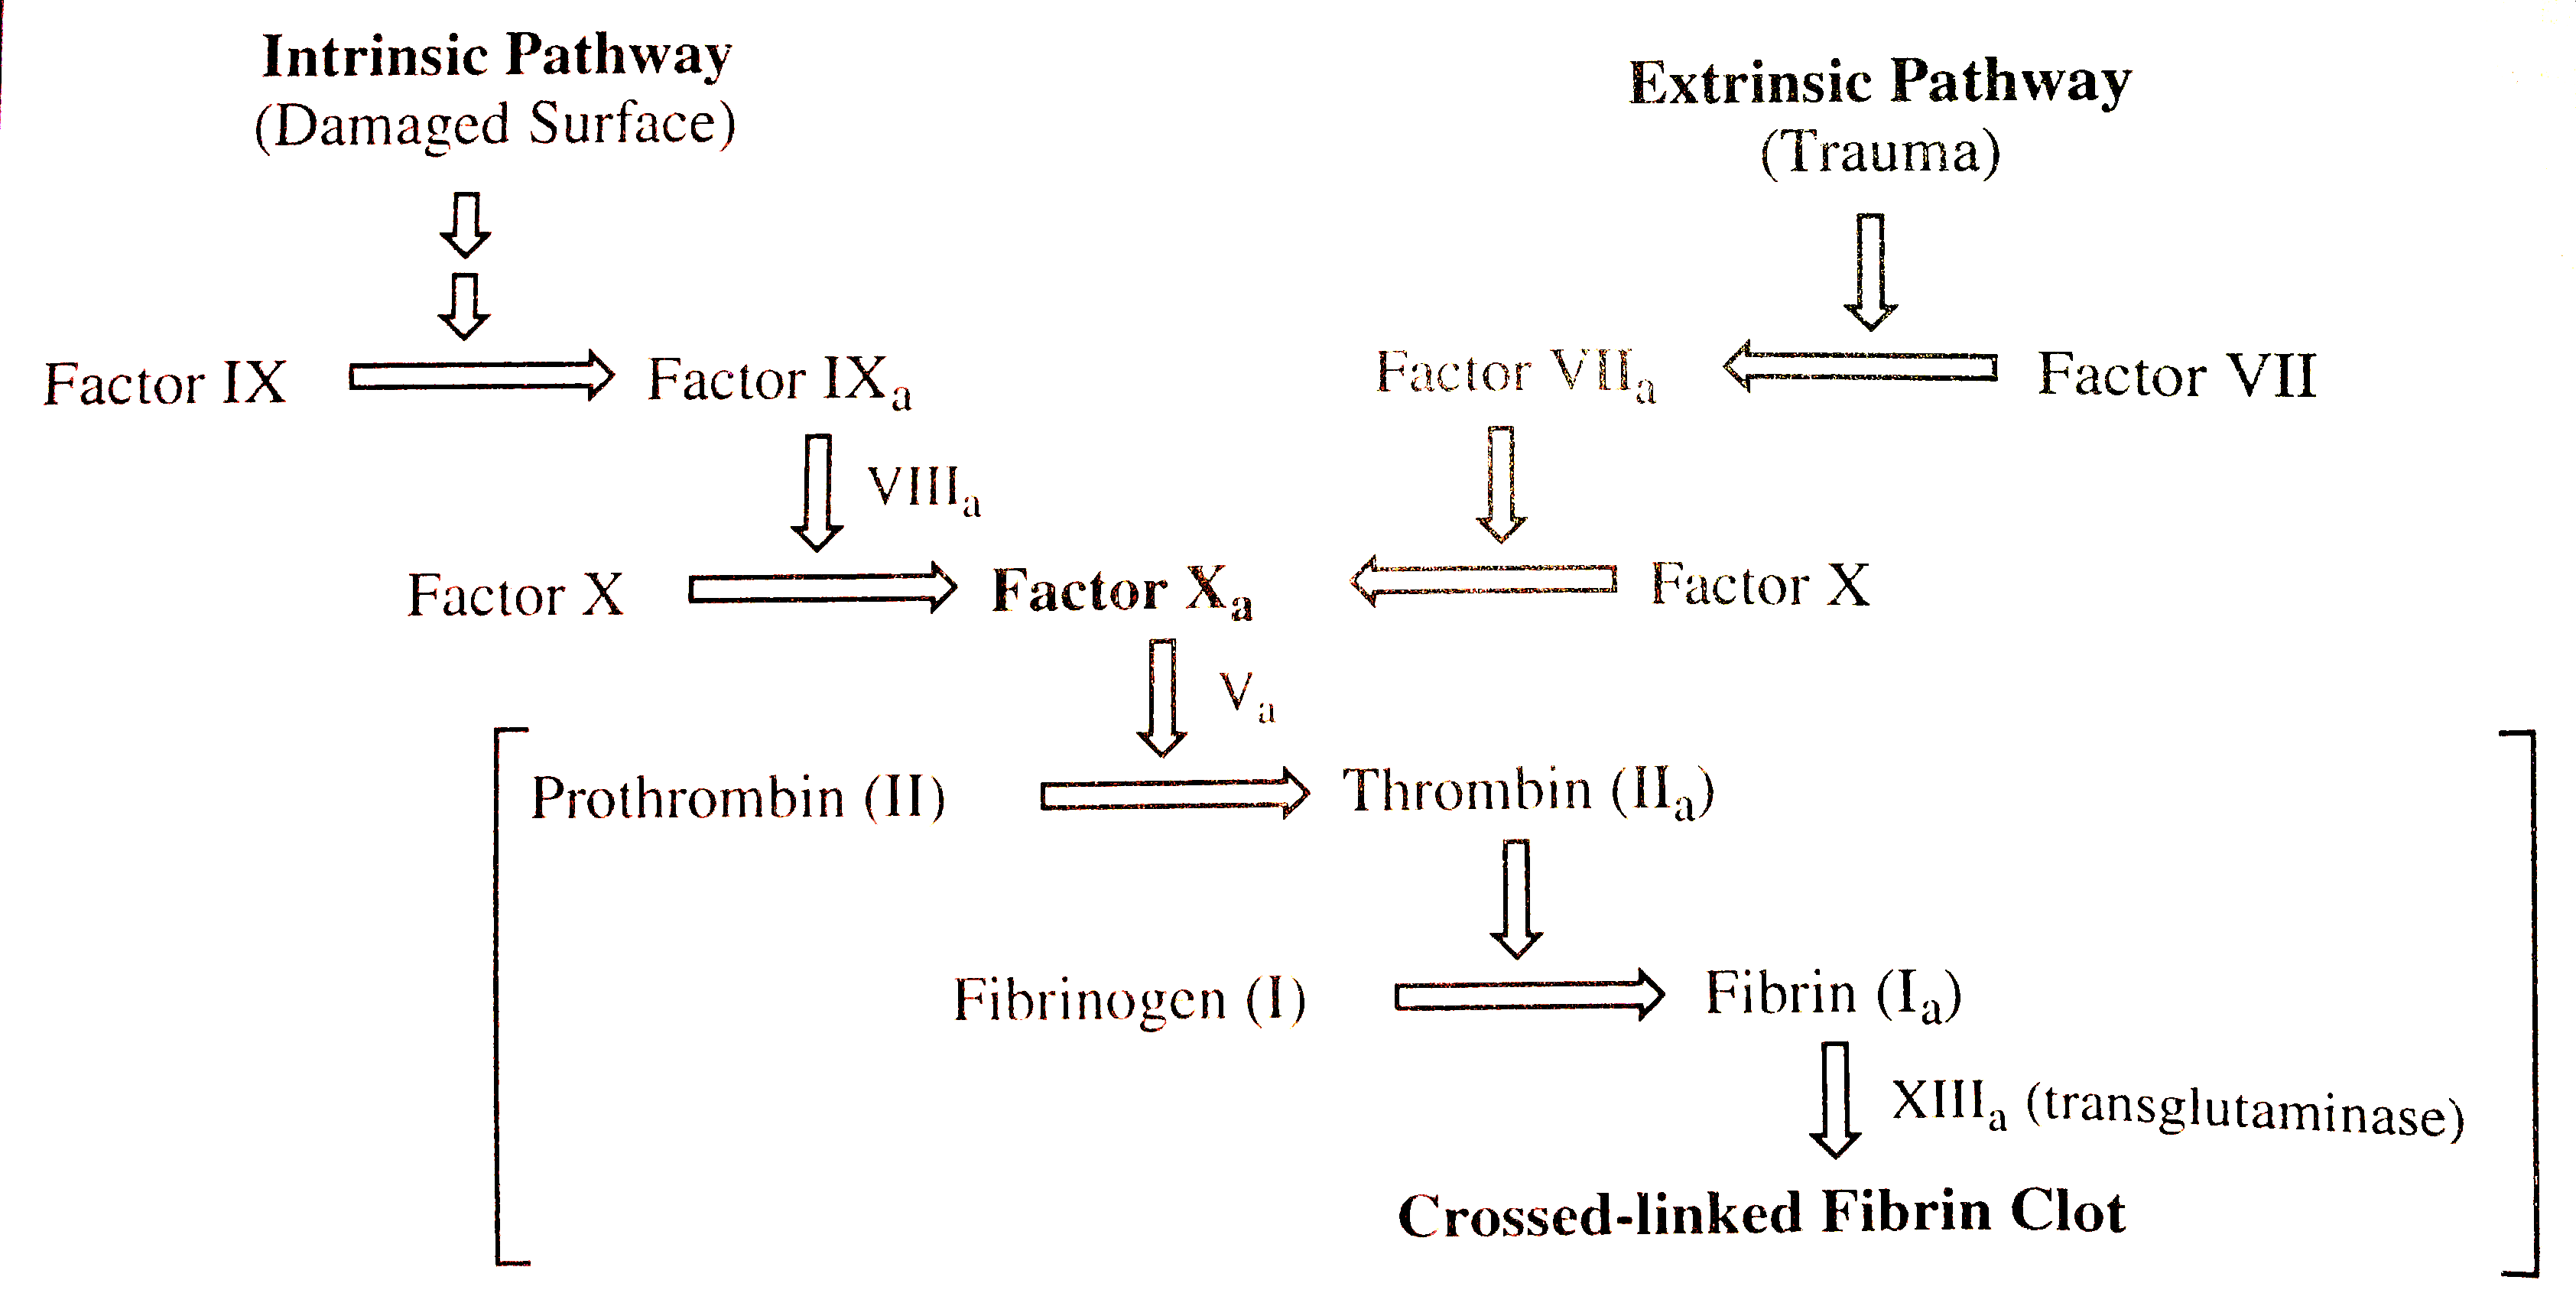
\includegraphics[width=0.7\textwidth]{blood_clotting.png} \label{blood_clotting}
\caption{The intrinsic and extrinsic pathways of blood clotting.}
\end{figure}
\noindent \textbf{Vitamin K} is a fat-soluble vitamin, and it is important for blood clotting. This is because prothrombin exists in an even earlier form called \textit{preprothrombin}, which has certain Glu residues that are carboxylated by a carboxylase enzyme. This carboxylase enzyme has an absolute requirement for Vitamin K. Therefore, in the presence of Vitamin K, \ce{HCO_{3}-}, and the carboxylase enzyme, we can convert preprothrombin to prothrombin. This structure now has great affinity for divalent ions such as \ce{Ca^2+}, and is therefore a good chelating agent. Therefore, the essentials for the clotting process to take place is the (a) platelet membrane, (b) enzymes, (c) \ce{Ca^2+}, (d) an auxiliary factor, Factor V\textsubscript{a}, and (e) the substrate prothrombin. \\
\indent Thrombin can now act as a proteolytic enzyme that converts \textit{fibrinogen} to \textit{fibrin}. Fibrinogen is a large soluble protein. Its solubility is due to an excess of negatively charged amino acids (i.e. Glu, Asp, Tyr-\ce{SO_4}), particularly in the central domain of the molecule. The net charge in the central domain of the fibrinogen is -8, while the net charge at the terminal ends is -4. In general, if very large molecules have a net charge of zero, they will tend to come together. However, if we have an excess of charge (as is the case with fibrinogen), the molecules will repel one another. Thus, in order to convert the soluble fibrinogen to the insoluble fibrin, we can remove the portion of the molecule contributing all the negative charge. Indeed, when fibrinogen is converted to fibrin, we find that 4 Arg-Gly bonds are broken in the central domain, releasing four peptides containing an excess of negative charge. Once these `fibrinopeptides' are released, the overall net charge in the central domain now becomes +5 (originally -8 in fibrinogen). The fibrin monomer that is now formed has the ability to interact with other fibrin monomers through electrostatic interactions between the terminal (negatively charged) and central (positively charged) regions of the polypeptide\textemdash the resulting aggregation is called a \textbf{fibrin (soft) clot}. \\
\indent To make the soft clot into a hard clot, the enzyme transglutaminase (Factor XIII\textsubscript{a}) cross-links the monomers. Once the damaged area has been repaired, a serine protease called \textbf{plasmin} hydrolyzes specific regions in the fibrin clot in order to dissolve it into smaller peptide fragments (to remove the clot). \textbf{Tissue plasminogen activator (TPA)} converts \textbf{plasminogen} into this active protease. 

\subsection{The Lungs}
When we breathe air, it first enters through the nose/mouth, passes from the oral cavity to the \textbf{pharynx}, into the \textbf{larynx}, and then down the \textbf{trachea}. At the end of the trachea, the air passes into two tubular passageways called \textbf{bronchi}. One bronchi enters into each lung and continues to divide into smaller passageways called \textbf{bronchioles}, eventually ending in the functional units of the lungs called the \textbf{alveoli}. Each alveolus consists of a single layer of epithelial cells juxtaposed to a very thin basement membrane. Surrounding each single alveolus is a capillary network.\\
\indent At equilibrium, the number the \ce{O2} molecules dissolving in water will equal the number of \ce{O2} molecules leaving the water. This means the partial pressure of oxygen in the gas phase (air) is equal to the partial pressure of oxygen in the liquid phase (water):
\begin{equation}
\begin{split}
\boxed{\left(P_{\text{O\textsubscript{2}}}\right)_{\text{gas}}=\left(P_{\text{O\textsubscript{2}}}\right)_{\text{liquid}}}
\end{split}
\end{equation}
\noindent The \textbf{epithelial cells} that line the lumen of the passageways to the end of the bronchioles have \textbf{cilia} which are continually beating towards the pharynx. Scattered among these epithelial cells are glands that secrete \textbf{mucus}, which is important to trap and foreign matter and get rid of it as the mucus is moved upward towards the oral cavity. The upper passageways of the respiratory tract maintain their opening by means of \textbf{cartilage rings}. Smooth muscle is found in almost all areas of the respiratory tract where there's no cartilage. \textbf{Asthma} is caused by allergic hypersensitivity to airborne antigens that have entered the respiratory tract. The direct result is to cause the mast cells within the bronchioles to release a number of different substances that cause the smooth muscle surrounding bronchioles to spasm and constrict. \\
\indent The lungs are encased in the pleural membrane. The \textbf{visceral pleura} covers the lungs, while the \textbf{parietal pleura} adheres to the diaphragm and chest wall. Between the visceral pleural and parietal pleura is the \textbf{intrapleural space} which contains a watery fluid. During inspiration, the muscles of the diaphragm contract and pull the diaphragm down, enlarging the thoracic cage and expanding the lungs. This creates a subatmospheric pressure in the alveoli, which causes air to rush down its pressure gradient from the atmosphere into the lungs. During expiration, the thoracic cage and lungs return to normal, and air in the alveoli is compressed and forced out through the passageways of the respiratory tract. If the lungs were to become separated from the visceral pleura, they would collapse, causing \textbf{pneumothorax}. This is because they have no anatomical structures to maintain rigidity. \\
\indent As deoxygenated blood comes back from the tissues, it enters the right atrium via the superior and inferior vena cava and passes into the right ventricle, where it is pumped to the lungs via the pulmonary artery. In the alveoli, both \ce{O_2} and \ce{CO_2} diffuse down their respective concentration gradients from the capillaries to the alveoli. This means that the oxygen enters the blood and carbon dioxide leaves the blood. The blood then becomes oxygenated, comes back to the heart via the pulmonary vein, and passes from the left atrium to the left ventricle and then pumped to the tissues via the aorta. Oxygen can travel/dissolve in the blood itself, but it's pretty insoluble in water/blood. Rather, most oxygen is transported by being bound to a transport protein in erythrocytes called \textbf{hemoglobin (Hb)}. Hb has four polypeptide units, each of which has a \textbf{heme} prosthetic group with an iron atom in the center in the ferrous \ce{Fe^2+} state. Thus, each hemoglobin molecule can take up to four \ce{O_2} molecules. \\
\indent Hb is dependent on pH and temperature\textemdash if we were to decrease the pH of the blood or increase the temperature, then less hemoglobin will be saturated with oxygen. This is what happens when you exercise. Similarly, this shift in the oxygen saturation curve happens when a byproduct of glycolysis, \textbf{2,3-bisphosphoglycerate (2,3-BPG)}, binds go hemoglobin.\\
\indent \ce{CO_2} can be carried in the blood by either (1) dissolving in the plasma and RBCs, (2) binding to a specific site on the hemoglobin molecule, or (3) in the form of bicarbonate ions (\ce{HCO_{3}-}). Most of the \ce{CO_2} is carried in the blood in the form of bicarbonate ions. 

\subsection{The Gastrointestinal Tract}
The gastrointestinal (GI) system includes the mouth and associated salivary glands, esophagus, stomach, small intestine, large intestine, and certain aspects of the liver and pancreas. Starch, characteristic of plant cells, and glycogen, characteristic of animal cells, are hydrolyzed within the digestive trace by \textbf{amylases}. Upon hydrolysis, both polymers release glucose. \textbf{Cellulose} is found within the cell walls of plants; the enzyme \textbf{cellulase} can hydrolyze cellulose into its constituent glucose residues.
\begin{equation}
\begin{split}
\text{Starch}\xrightarrow[\textbf{Amylase}]{} \text{Glucose}, \quad \text{Cellulose}\xrightarrow[\textbf{Cellulase}]{\text{An example of bacterial symbiosis}} \text{Glucose}
\end{split}
\end{equation}
\noindent \textbf{Proteases} can hydrolyze proteins to their constituent amino acid residues. Of the 20 canonical amino acids, we need to obtain 9 of them in our diet, which are thus referred to as \textbf{essential amino acids}. The rest we can synthesize ourselves. Fat cellls (adipocytes) store triacylglycerols (i.e. fats) that are hydrolyzed into fatty acids and glycerol by the enzyme \textbf{lipase}.\\
\indent In the small intestine, the innermost layer is a convoluted layer of epithelial cells, with endocrine cells and ducts from external exocrine glands like the pancreas and liver scattered throughout that can release hormones into the blood and influence other cells in the GI tract. Both the parasympathetic and sympathetic nerves of the autonomic nervous system innervate the GI system; the more important nerves stem from the \textbf{parasympathetic} system. Recall that the parasympathetic nerves are more active during times of relaxation and digestion, while the sympathetic nerves are more active during times of `fight or flight.' \\
\indent As food is swallowed and passed into the pharynx, access to the nasal cavity is closed; a flap of tissue called the \textbf{epiglottis} covers the opening to the \textbf{larynx} and prevents food from entering into this passageway to protect the airway. The swallowing reflex is controlled by centers in the medulla. \\
\indent As food boluses pass through, the smooth muscles surrounding the epithelial cells contract in perstaltic waves, and this is referred to as \textbf{peristalsis}, controlled by the action of the parasympathetic division and by the action of hormones. \\
\indent Once the food reaches the stomach, a \textit{sphincter} (circular muscle) called the \textbf{gastroesophageal sphincter} contracts and prevents regurgitation of the food back into the esophagus. If this sphincter were not closed off, stomach acid would enter the esophagus and irritate the nerve endings in the smooth muscle, causing a burning sensation referred to as heartburn. In the stomach, there are four major types of secretion. \textbf{Mucus} is secreted by \textbf{surface cells} and acts to protect the lining of the stomach and lubricate the food. \textbf{Gastrin}, located in the endocrine cells in the lower portion of the stomach, is secreted in response to protein entering into the stomach. This hormone stimulates the secretion of \ce{HCl} and pepsinogen. \textbf{\ce{HCl}} at a pH of about 1 is secreted by \textbf{parietal cells}, while \textbf{pepsinogen} is secreted by the \textbf{chief cells}. Parietal cells and chief cells are located in the \textbf{gastric pits} that line the epithelium of the stomach. Pepsinogen is the inactive form of the peptidase enzyme \textbf{pepsin} that becomes activated by \ce{HCl} and also by a positive feedback loop and auto-activation once pepsinogen reaches the stomach. \\
\indent In addition to secreting \ce{HCl}, the parietal cells also secrete a glycoprotein called \textbf{intrinsic factor}. This glycoprotein is important because it complexes with vitamin B\textsubscript{12} and is then absorbed by the intestinal epithelial cells and transported by the bloodstream. Vitamin B\textsubscript{12} is important in erythrocyte formation. If too much acid is secreted into the stomach, \textbf{ulcers} can occur in the stomach and small intestine. Ulcers are erosions of the walls of these organs, and if they are extensive, they can cause bleeding. \textbf{Histamine} is a powerful stimulant that causes \ce{HCl} to be released into the lumen of the stomach, and so compounds like \textbf{cimetidine} inhibit the binding of histamine to its receptor on parietal cells. This effectively reduces the amount of \ce{HCl} secreted in the lumen of the stomach. \\
\indent Roughly $90\%$ of digestion and absorption that takes place in the GI tract occurs in the small intestine, which acts to neutralize the acid which has been secreted by the stomach and to further digest and absorb food particles. Distension of the small intestine also causes the hormone \textbf{cholecystokinin (CCK)} to be released from the intestinal mucosa. CCK diffuses through the bloodstream to the pancreas where it causes the pancreas to release digestive enzymes. The hormone \textbf{secretin} is released from the small intestine in response to the entering chyme from the stomach. Secretin is also absorbed by the blood and is transported to the pancreas where it causes the release of bicarbonate ion and other fluids.\\
\indent The \textbf{pancreas} not only has endocrine cells that secrete insulin and glucagon, but also contains secreting structures called \textbf{acini} that secrete a fluid into the small intestine which has a high \textbf{bicarbonate} conent that is rather alkaline, which reacts with the stomach acid to product carbonic acid, which then decomposes into carbon dioxide and water. \\
\indent The liver has many functions, one of which is to synthesize \textbf{bile} that is concentrated and stored in the \textbf{gallbladder}. Bile contains a major pigment called \textbf{bilirubin}, which is the breakdown product of hemoglobin. It also contains \textbf{bile salts} which are important in the digestion and absorption of fats. When bile is released from the gallbladder, it passes down a duct that joins with the pancreatic duct, through a constriction called the \textbf{sphincter of Oddi}, and empties into the small intestine. Bile acts to emulsify fats, which basically means just decreasing their surface tension in order to break them up into smaller sizes, making it easier to absorb. The presence of fats in the small intestine releases CCK which then acts on the gallbladder and causes contraction, and on the sphincter of Oddi and causes relaxation, so the bile can pass into the lumen of the small intestine. \\
\indent Remember that the \ce{Na+}-glucose symport is on the apical side of the epithelial cells in the small intestine (the side facing the lumen), while the \ce{Na+}-\ce{K+} antiport pump is on the basolateral side facing the blood. There's also a glucose passive transporter on the basolateral side to allow glucose to naturally enter the blood according to its concentration gradient. This is shown in \textbf{Fig. \ref{transport_systems}}.\\
\begin{figure}[!ht]
\centering
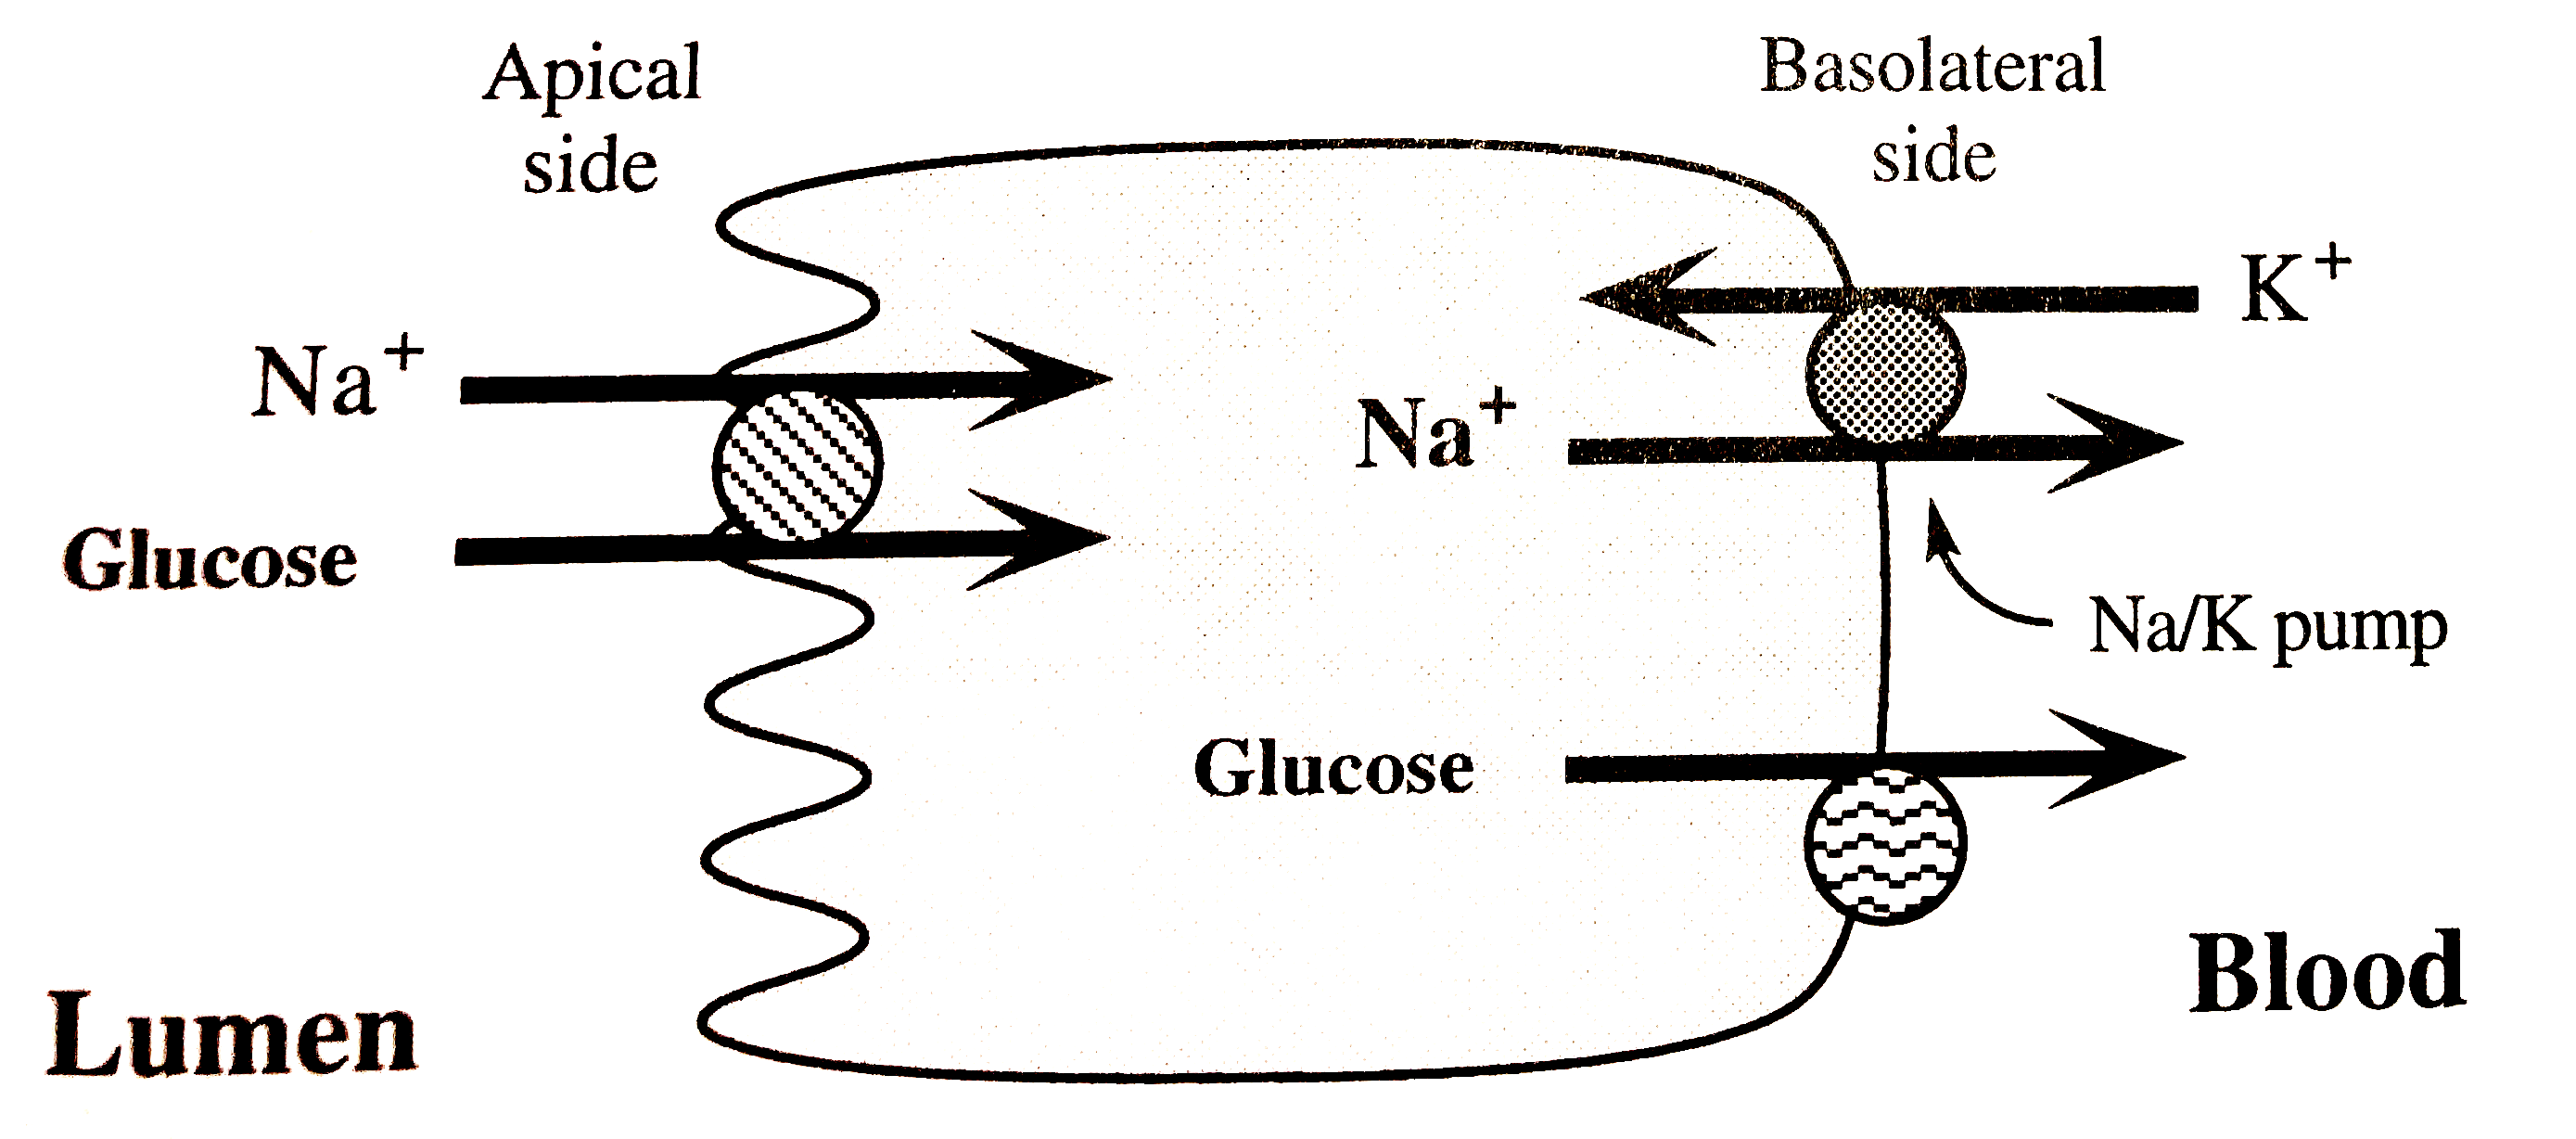
\includegraphics[width=0.7\textwidth]{transport_systems.png} \label{transport_systems}
\caption{Transport systems.}
\end{figure}
\indent Recall that fats are degraded to fatty acids and glycerol by the lipase enzyme. These compounds can diffuse into the intestinal epithelial cells where they are resynthesized into triglycerides (fats) and aggregate into structures called \textbf{chylomicrons}. These aggregates are released at the basolateral membrane and into the extracellular space, and enter the lymph and are transported to the veins and eventually the tissues.\\
\indent The large intestine absorbs most of the water and ions that are left in the chyme as it passes from the small intestine. As the sodium and chloride ions are absorbed, an osmotic gradient is established that allows for the absorption of water. What is not absorbed is passed out of the body in the feces.

\subsection{The Kidney}
Water can be lost from the \textbf{integument} (i.e. the skin) by evaporation, the GI tract, the lungs, and the urinary system. Recall that osmolarity refers to the total solute concentration of a solution. Remember, the higher the osmolarity of a given solution, the lower will be the concentration of water in that solution.\\
\indent If an organism can change the internal ionic concentration of its fluids to meet that of the surrounding environment are referred to as \textbf{osmoconformers}; many marine invertebrates are osmoconformers. However, most vertebrates do not change the internal ionic concentration of their body fluids to meet that of a surrounding environment. Organisms like this are referred to as \textbf{osmoregulators}. \\
\indent Kidneys have three main functions: filtration, reabsorption, and excretion.
\begin{enumerate}
	\item \textbf{Filtration:} The functional unit in the kidney is the \textbf{nephron} which consists of a \textbf{glomerulus}, \textbf{Bowman's capsule}, and a \textbf{tubular} system. The glomerulus is a collection of capillaries that receives blood from an artery terminating in the renal system. Blood is pumped into the glomerulus by the hydrostatic pressure of the heart, and that pressure forces the blood through the capillary walls and into Bowman's capsule. The cell-free ultrafiltrate found in Bowman's capsule lacks many of the plasma proteins found in the blood. Blood \textbf{plasma} is simply a solution which is about $90\%$ water that is composed of organic (i.e. proteins, sugars, amino acids, etc.) and inorganic substances (i.e. various ions like sodium and chloride). There's also erythrocytes, lymphocytes, and platelets. The \textbf{filtrate} in Bowman's capsule is essentially the plasma minus the large MW proteins.
	\item \textbf{Reabsorption:} The kidney also reabsorbs important organic and inorganic compounds from the filtrate in Bowman's capsule. Reabsorption occurs through many of the epithelial cells which line the tubular lumen of the nephron. The \textbf{cilia} of these epithelial cells move in such a way as to help propel the filtrate through these renal tubes. Glucose, small proteins, amino acids, salts, bicarbonate ions, and water are reabsorbed along this tubular system and transported back into the blood. This epithelial cells also have the ability to secrete protons, potassium, urea, uric acid, and ammonia.
	\item \textbf{Excretion:} The kidney also helps excrete waste, salts, and excess water. 
\end{enumerate}
\noindent Blood from the descending aorta enters into the \textbf{renal artery} and eventually into the \textbf{glomeruli} of the nephrons. Blood leaves the kidney by way of the \textbf{renal vein} which itself empties into the inferior vena cava. Leaving each kidney is a \textbf{ureter} which transports the urine to the \textbf{bladder}. Urine exits the bladder by way of the \textbf{urethra}. Each kidney contains more than a million nephrons. The glomerulus and Bowman's capsule of each nephron is located in the \textbf{cortex} and gives this portion of the kidney a \textbf{granular} appeareance. In contrast, the \textbf{striated} appearance of the \textbf{medulla} is primarily due to a portion of the system of the nephron called the \textbf{loop of Henle} and the \textbf{collecting duct}. The collecting ducts, which collect the urine, empty into the renal pelvis of the kidney and then into the ureter. \\
\indent The functional unit of the kidney is the \textbf{nephron}. As the \textbf{renal artery} branches into smaller division and enters the kidney, it becomes the \textbf{afferent arteriole}, which then enters into the \textbf{Bowman's capsule} and forms the capillary bed called the \textbf{glomerulus}. An \textbf{efferent arteriole} leaves the glomerulus and forms a capillary network which surround the renal tubules. The blood that leaves this capillary network does so by a \textbf{venule} which later empties into the \textbf{renal vein} that leaves the kidney. Extending from Bowman's capsule is a long tubular structure divided into the \textbf{proximal convoluted tubule (PCT)}, \textbf{loop of Henle}, \textbf{distal convoluted tubule (DCT)}, and the \textbf{collecting duct}. Many different nephrons can attach to a single collecting duct. The anatomy of the nephron is shown in \textbf{Fig. \ref{nephron}}.\\
\begin{figure}[!ht]
\centering
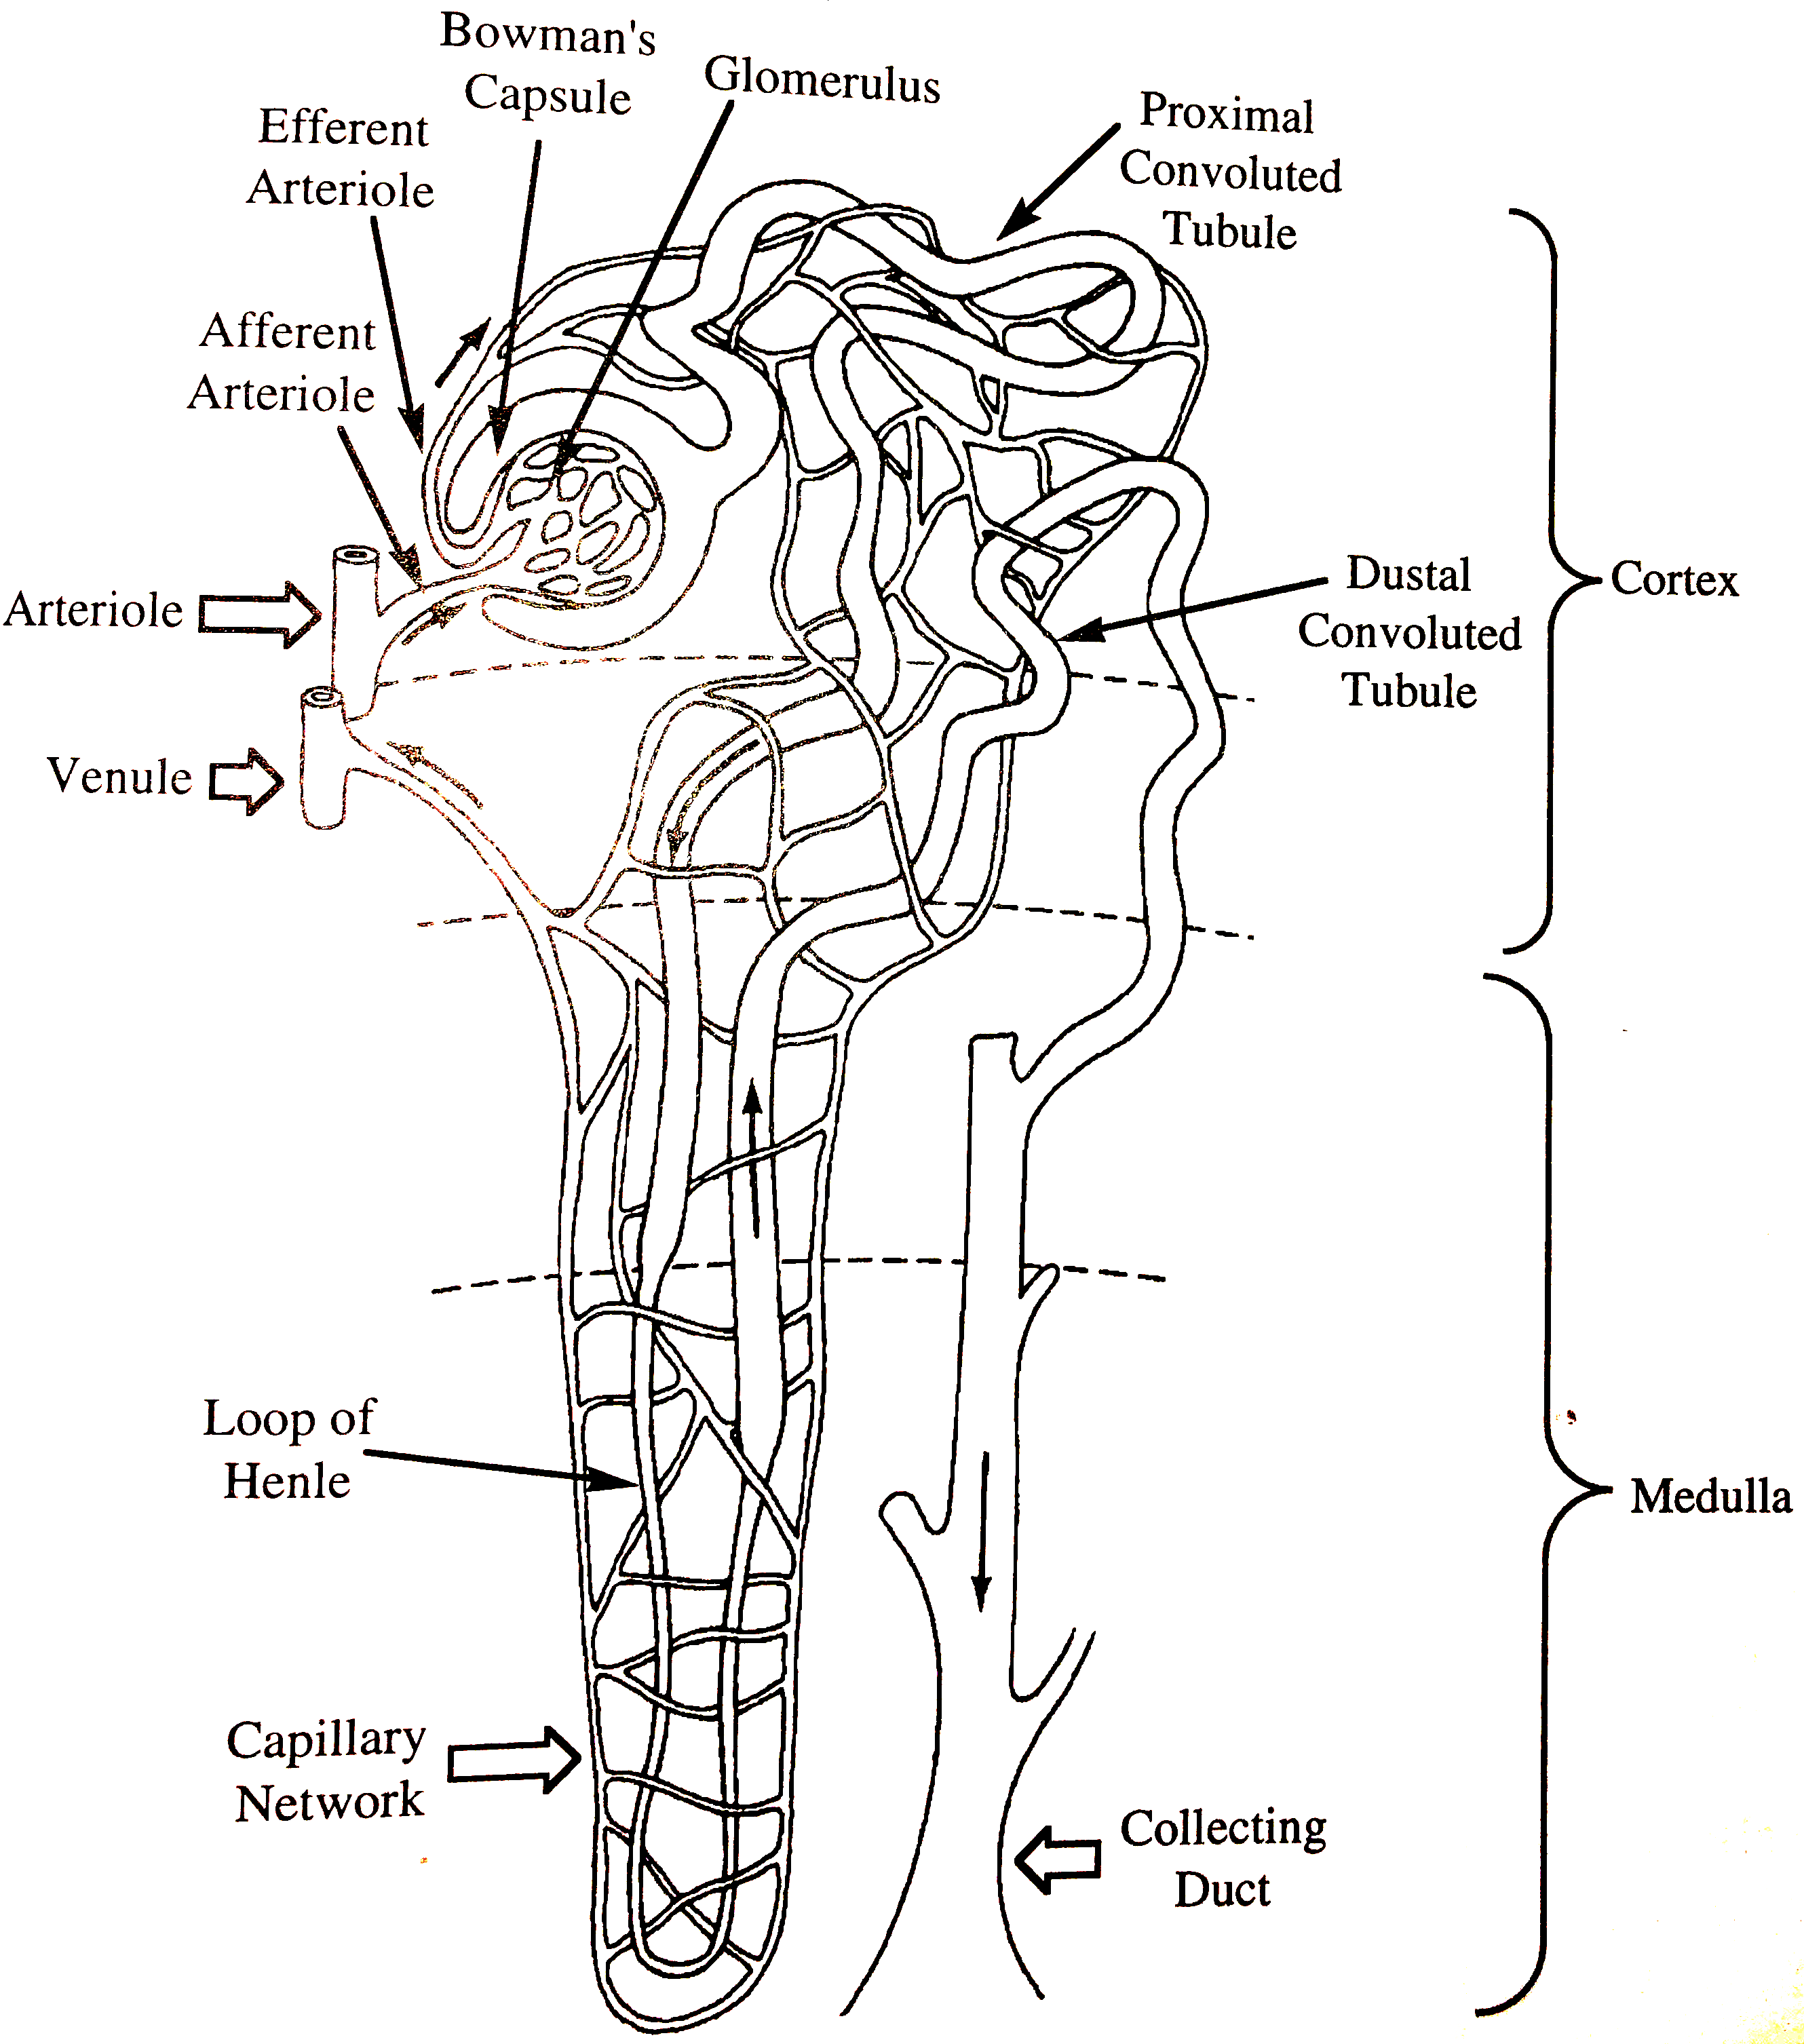
\includegraphics[width=0.7\textwidth]{nephron.png} \label{nephron}
\caption{The nephron and its related capillary system.}
\end{figure}
\indent The PCT is the \textit{obligatory} section of the nephron because roughly $65\%$ of all reabsorption and secretion occurs here. Little regulation occurs in the PCT. Glucose, small MW proteins, amino acids, and vitamins are \textit{completely} reabsorbed in the PCT, and roughly $80\%$ of \ce{Na+}, \ce{Cl-}, and water are reabsorbed in the PCT. As the PCT begins to descend from the cortex into the medulla, it forms the loop of Henle, which has a thin portion and thick portion. The descending thin portion is very permeable to water but only relatively permeable to ions and molecules. The ascending thin portion is the reverse. As the loop of Henle ascends it becomes thicker. The epithelial cells in this region actively transport ions like \ce{Na+} and \ce{K+} from the lumen of the loop into the interstitial fluid. However, this region is impermeable to urea and water. The filtrate from the thick portion of the loop of Henle passes into the DCT, which is also impermeable to urea and water but rather permeable to ions. The filtrate becomes even more dilute. The DCT epithelial cells and the collecting duct cells located in the cortical region of the kidney are quite sensitive to \textbf{aldosterone} secreted by the adrenal glands. An increase in aldosterone causes sodium to be reabsorbed by the epithelial cells. These cells also respond to \textbf{antidiuretic hormone (ADH)}, produced by the hypothalamus and released by the posterior pituitary. If the concentration of ADH increases, then water will be reabsorbed from the epithelial cells in the collecting duct and passed to the interstitial space. The cells of the collecting duct can also secrete hydrogen ions (as can the cells of the PCT and DCT).\\
\indent The osmolarity of the filtrate in Bowman's capsule is essentially the same osmolarity in the plasma. 

\subsection{Homeostatic Mechanisms}
Suppose we want to maintain the levels of sodium in the body. Certain cells in the cortex of the adrenal gland are sensitive to the levels of sodium in the blood. When the concentration of \ce{Na+} \textit{decreases} in the blood, these cells release the hormone \textbf{aldosterone}, which acts at the level of the \textbf{DCT} (distal convoluted tubule) and the \textbf{collecting ducts} and stimulates the epithelial cells in those regions to reabsorb sodium. As a result, the blood concentration of sodium begins to rise. This acts as a signal and feeds back on the cortical cells of the adrenal gland, telling it to reduce the secretion of aldosterone.\\
\indent Suppose we want to maintain the proper levels of water in the body. If there's a \textit{decrease} in the plasma volume of the body, there will be a lower blood pressure (detected by baroreceptors) but a higher osmotic pressure (detected by osmoreceptors). These receptors would stimulate specific cells in the hypothalamus to synthesize and transmit \textbf{ADH} (anti-diuretic hormone) to the posterior pituitary where it is released into the blood. ADH stimulates the epithelial cells in the latter portion of the \textbf{DCT} and collecting ducts to absorb water. This leads to less water excretion and a higher plasma volume. If you were to drink too much water, then the opposite process would happen and you would excrete copious amounts of urine.\\
\indent We also should talk about nitrogenous wastes. Proteins and nucleic acids are the two primary metabolic sources of nitrogenous wastes, and can be removed as ammonia, urea, or uric acid. Ammonia is toxic and soluble, urea is less-toxic and soluble, and uric acid is toxic and insoluble. Fish metabolize glutamine into ammonia, which can be easily carried away with the passing water. Urea is excreted by most mammals, amphibians, and some reptiles and birds. The ammonia that is produced from the metabolism from the amino acids Gly, Asp, and Glu can be converted to uric acid, which is the primary excretory product of birds and reptiles. \\
\indent The normal pH of the body is 7.4. Anything below 7.35 or above 7.45 could be fatal if left for an extended period of time. Blood pH is regulated by a \textbf{buffering system} that involves bicarbonate: \ce{H+ + HCO_3- <-> H_2CO_3 <-> CO_2 + H_2O}.\\
\indent Recall that the cholera toxin is cased by the bacterium \textit{Vibro cholerae} and causes the rapid loss of fluid. According to the buffer system above, the loss of bicarbonate results in a shift of the bicarbonate buffer system to the side of the acid (\ce{H+}). If the volume of enteric fluid that is lost is large enough to overwhelm the ability of the kidney to regulate the proper acid-base levels in the body, \textbf{metabolic acidosis} results. An adult with severe untreated cholera in the blood pH can drop to a more acidic value of 7.19. To try to compensate, a clinical feature of metabolic acidosis is \textbf{hyperventilation} to try to eliminate the increased \ce{CO_2} more quickly, as by lowering the concentration of \ce{CO_2} in the body, the levels of \ce{H+} are also lowered. 

\subsection{Male Reproduction}
From an endocrinology standpoint, we have the following pathway:
\begin{equation}
\begin{split}
\text{Hypothalamus releases GnRH} \rightarrow \text{Anterior Pituitary releases LH and FSH} \rightarrow \text{Gonads produce steroids and germ cells}
\end{split}
\end{equation}
\noindent Note that this general signaling pathway applies to both males and females. \textbf{GnRH} is the \textbf{gonadotropin releasing hormone}, \textbf{LH} is \textbf{luteinizing hormone}, and \textbf{FSH} is follicle stimulating hormone. Both LH and FSH are called \textbf{gonadotropins}. In males, the germ cells ultimately produced are called \textbf{spermatozoa}, while in the female they are the \textbf{ova}. The male reproductive anatomy is shown in \textbf{Fig. \ref{male_reproductive_anatomy}}. 
\begin{figure}[!ht]
\centering
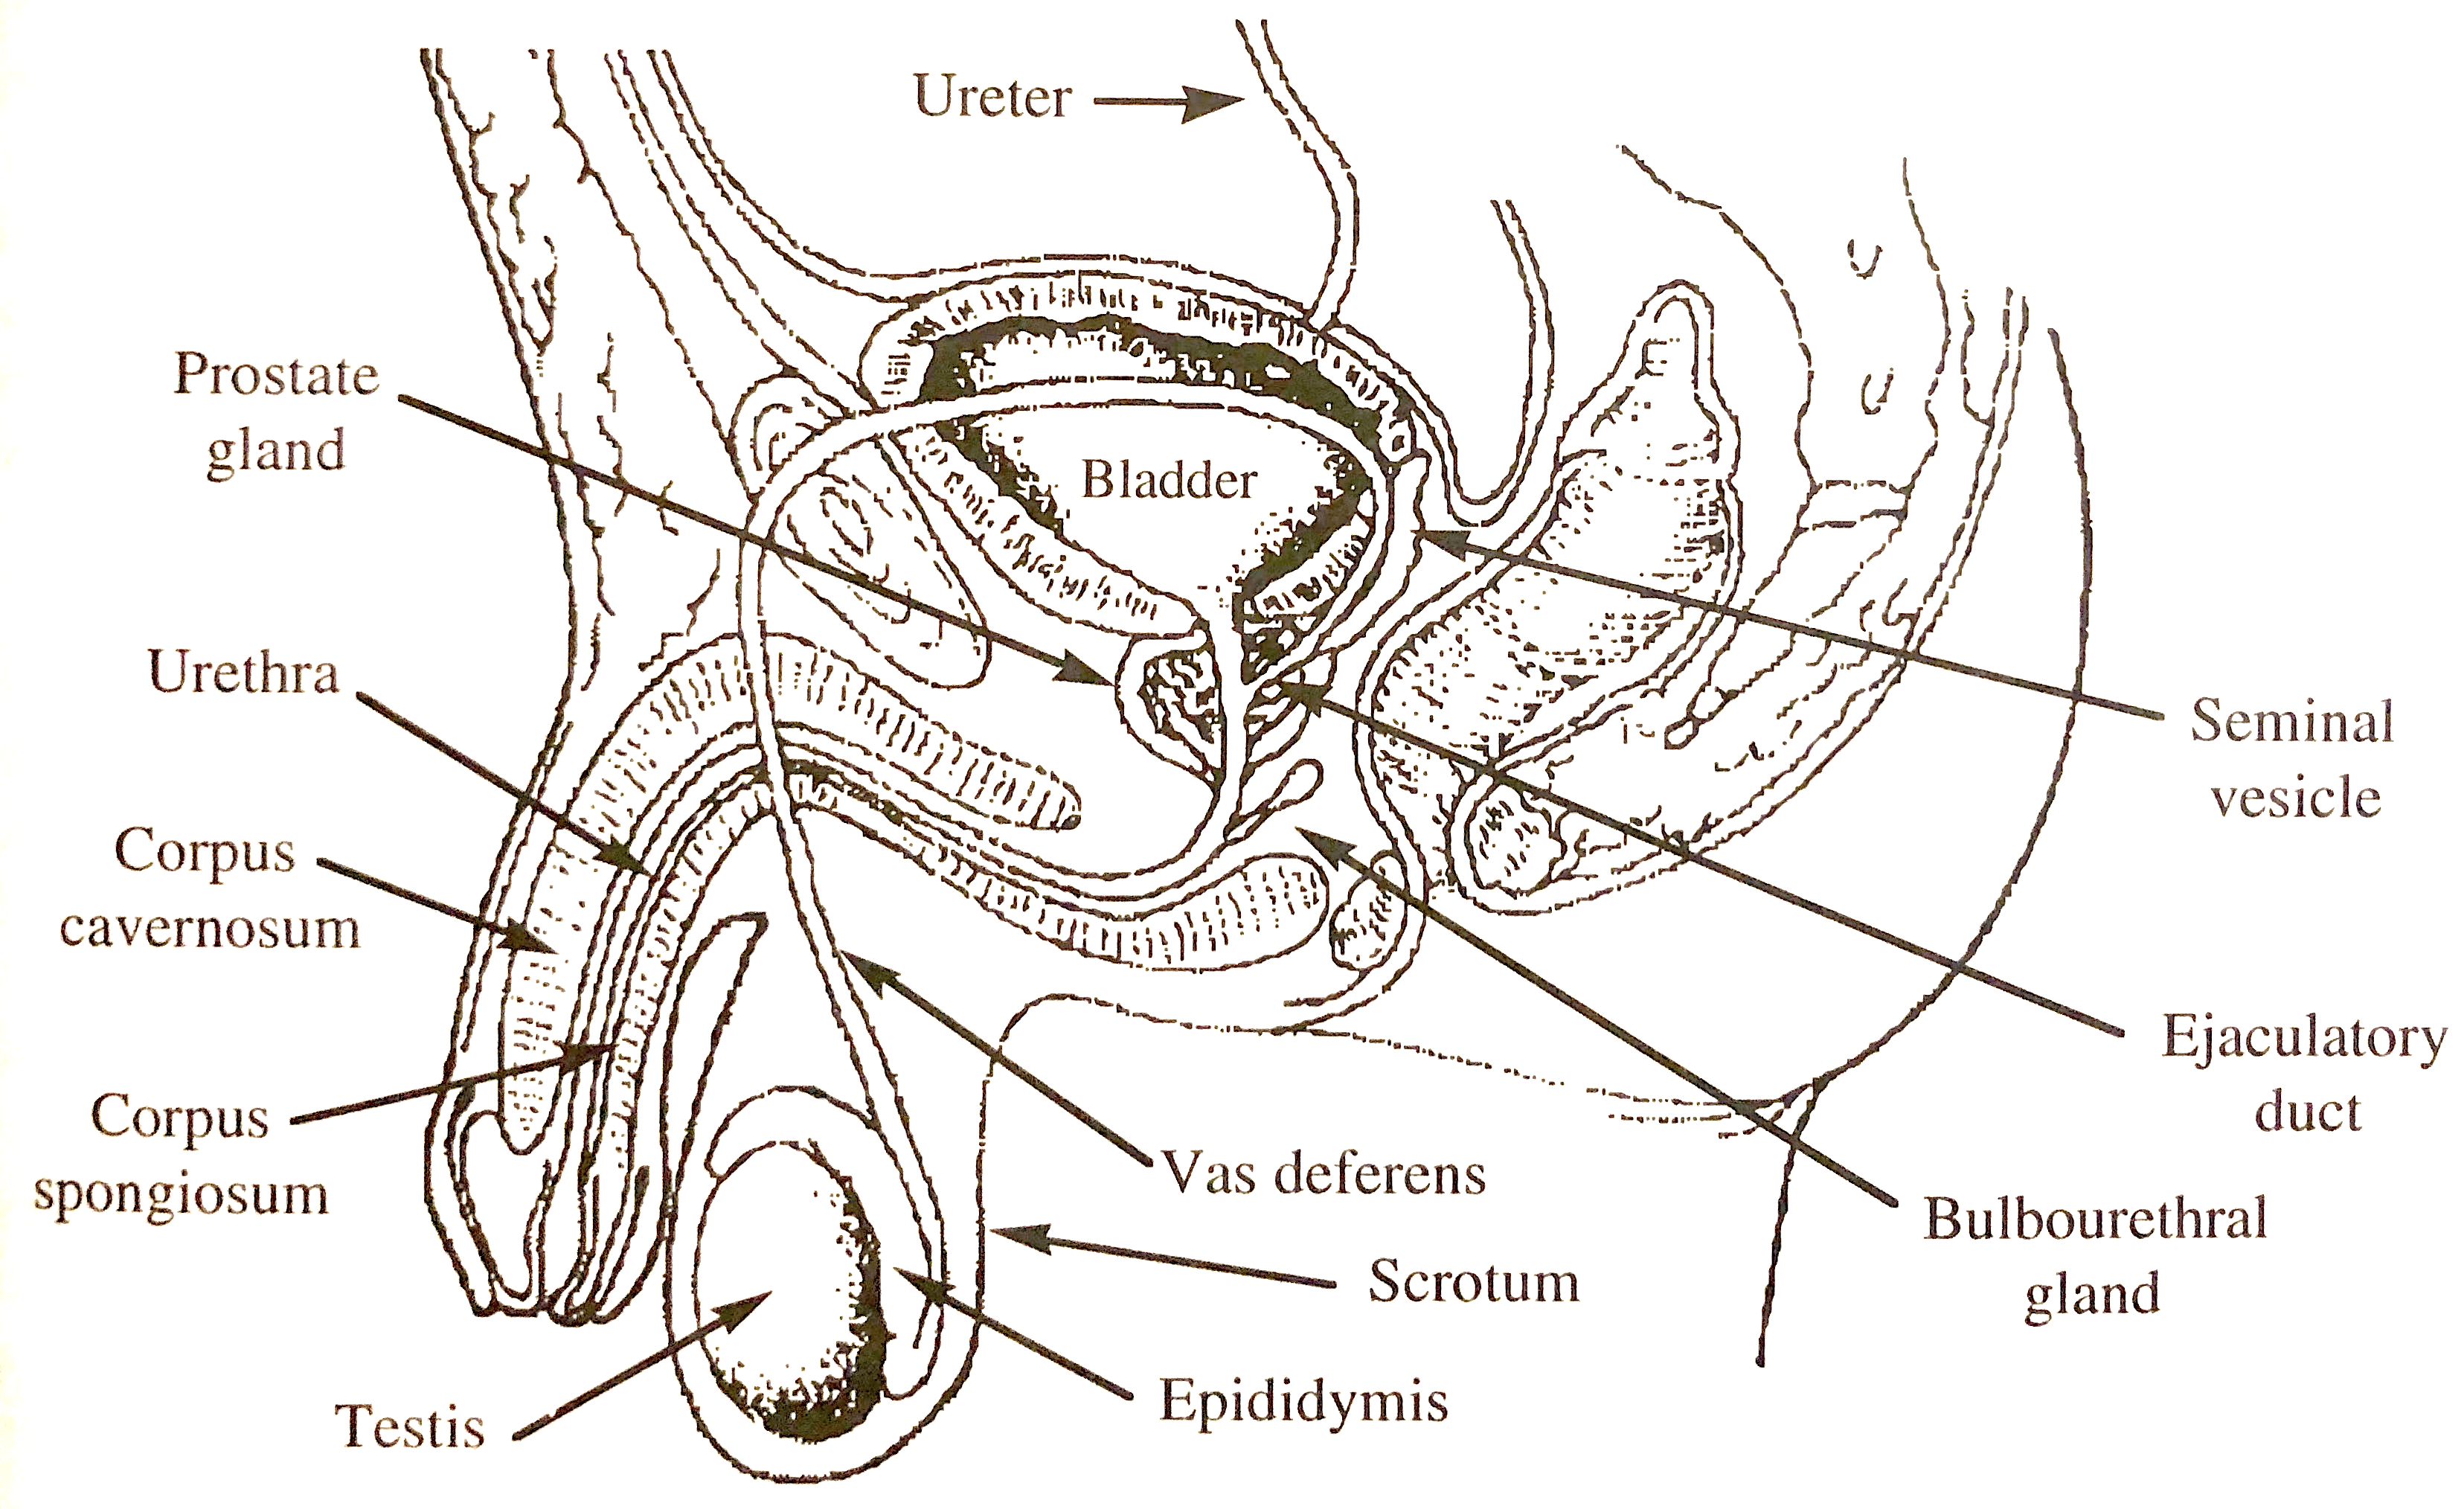
\includegraphics[width=0.7\textwidth]{male_reproductive_anatomy.png} \label{male_reproductive_anatomy}
\caption{Male reproductive anatomy.}
\end{figure}
\noindent Because spermatogenesis requires a lower temperature than that of the body, they are produced in the testes that lie in the scrotum outside the body cavity. Within each testis are a series of convoluted tubules celled the \textbf{seminiferous tubules}, and each of these tubules has the \textbf{spermatogenic cells}. The testes also produce the hormone \textbf{testosterone} using specialized interstitial cells called \textbf{Leydig cells} (also called the \textbf{interstitial cells}) that lie outside the seminiferous tubules. There are also \textbf{Sertoli cells} that lie outside the area of the seminiferous tubule, which promote spermatogenesis and produce the protein hormone \textbf{inhibin}. The Sertoli cells are in direct contact with the spermatogenic cells, and are adjacent to the lumenal space. \\
\indent Usually, the \textbf{spermatogonia} far away from the lumen of the seminiferous tubules will divide via mitosis. However, as they get closer and closer to the lumen, eventually they are referred to as \textbf{primary spermatocytes} and begin to undergo meiosis, thus producing \textbf{secondary spermatocytes} after the first meiotic division and \textbf{spermatids} after the second meiotic division, which now have half as many chromosomes. The spermatids then transform into the \textbf{spermatozoa}, which are released into the lumen.\\
\indent At the very tip of a spermatozoan, there is a structure called the \textbf{acrosome} which contains a lot of digestive enzymes that help the spermatozoa gain access to the interior of the egg once fertilization has taken place. Inside the head of the spermatozoa is a nucleus which contains the DNA. In the midsection are \textbf{mitochondria}, providing energy for the whipping movement of the tail to allow the sperm to swim towards their destination (i.e. the egg). \\
\indent The Leydig cells produce testosterone by converting cholesterol to it. Testosterone can (1) diffuse out of the Leydig cells and move to other target tissues of the body, (2) diffuse into the nearby Sertoli cells, which convert testosterone into \textbf{dihydrotestosterone (dHT)}. dHT diffuses into the nucleus of the Sertoli cell and causes transcription that ultimately affects the spermatogenic cells.\\
\indent LH (luteinizing hormone) binds to a specific receptor on the membrane of the Leydig cell, and causes the increase of the conversion of cholesterol into testosterone. Meanwhile, FSH (follicle stimulating hormone) binds to a surface receptor on the Sertoli cell that causes (1) an increase in the conversion of testosterone into dHT and (2) an increase in the synthesis of these FSH-sensitive receptors.\\
\indent Testosterone has a \textit{negative} feedback at the anterior pituitary and the hypothalamus, so it's important that it's able to diffuse out of the Leydig cells and enter the bloodstream. Specifically, it prevents the synthesis of GnRH and LH. Meanwhile, the Sertoli cells secrete a protein hormone called \textbf{inhibin}, which acts as a negative modulator of the anterior pituitary. Thus, if testosterone levels are too high, the feedback mechanism will decrease the levels of LH. If the levels of dHT are too high, there is an increase in inhibin synthesis that results in the decrease in FSH levels.\\
\indent Almost all of the secondary sex characteristics in the male are due to testosterone. After sperm is produced, they leave the seminiferous tubules and entire into the \textbf{epididymis} and then the \textbf{vas deferens}. Sperm is stored in these regions for about 14 days before ejaculation. Contraction of smooth muscle lining the walls of these structures ejects the sperm down the vas deferens and into the \textbf{ejaculatory duct}. The \textbf{seminal vesicles}, \textbf{prostate gland}, and \textbf{bulbourethral gland} secrete components that make the remainder of the fluid that is ejaculated (now called \textbf{semen}). Some of the components secreted by these glands are fructose vitamins, bicarbonate zinc, prostaglandins, and mucus. Overall, \textbf{Fig. \ref{testes_hormones}} shows us the general hormone involvement in the regulation of testes function.
\begin{figure}[!ht]
\centering
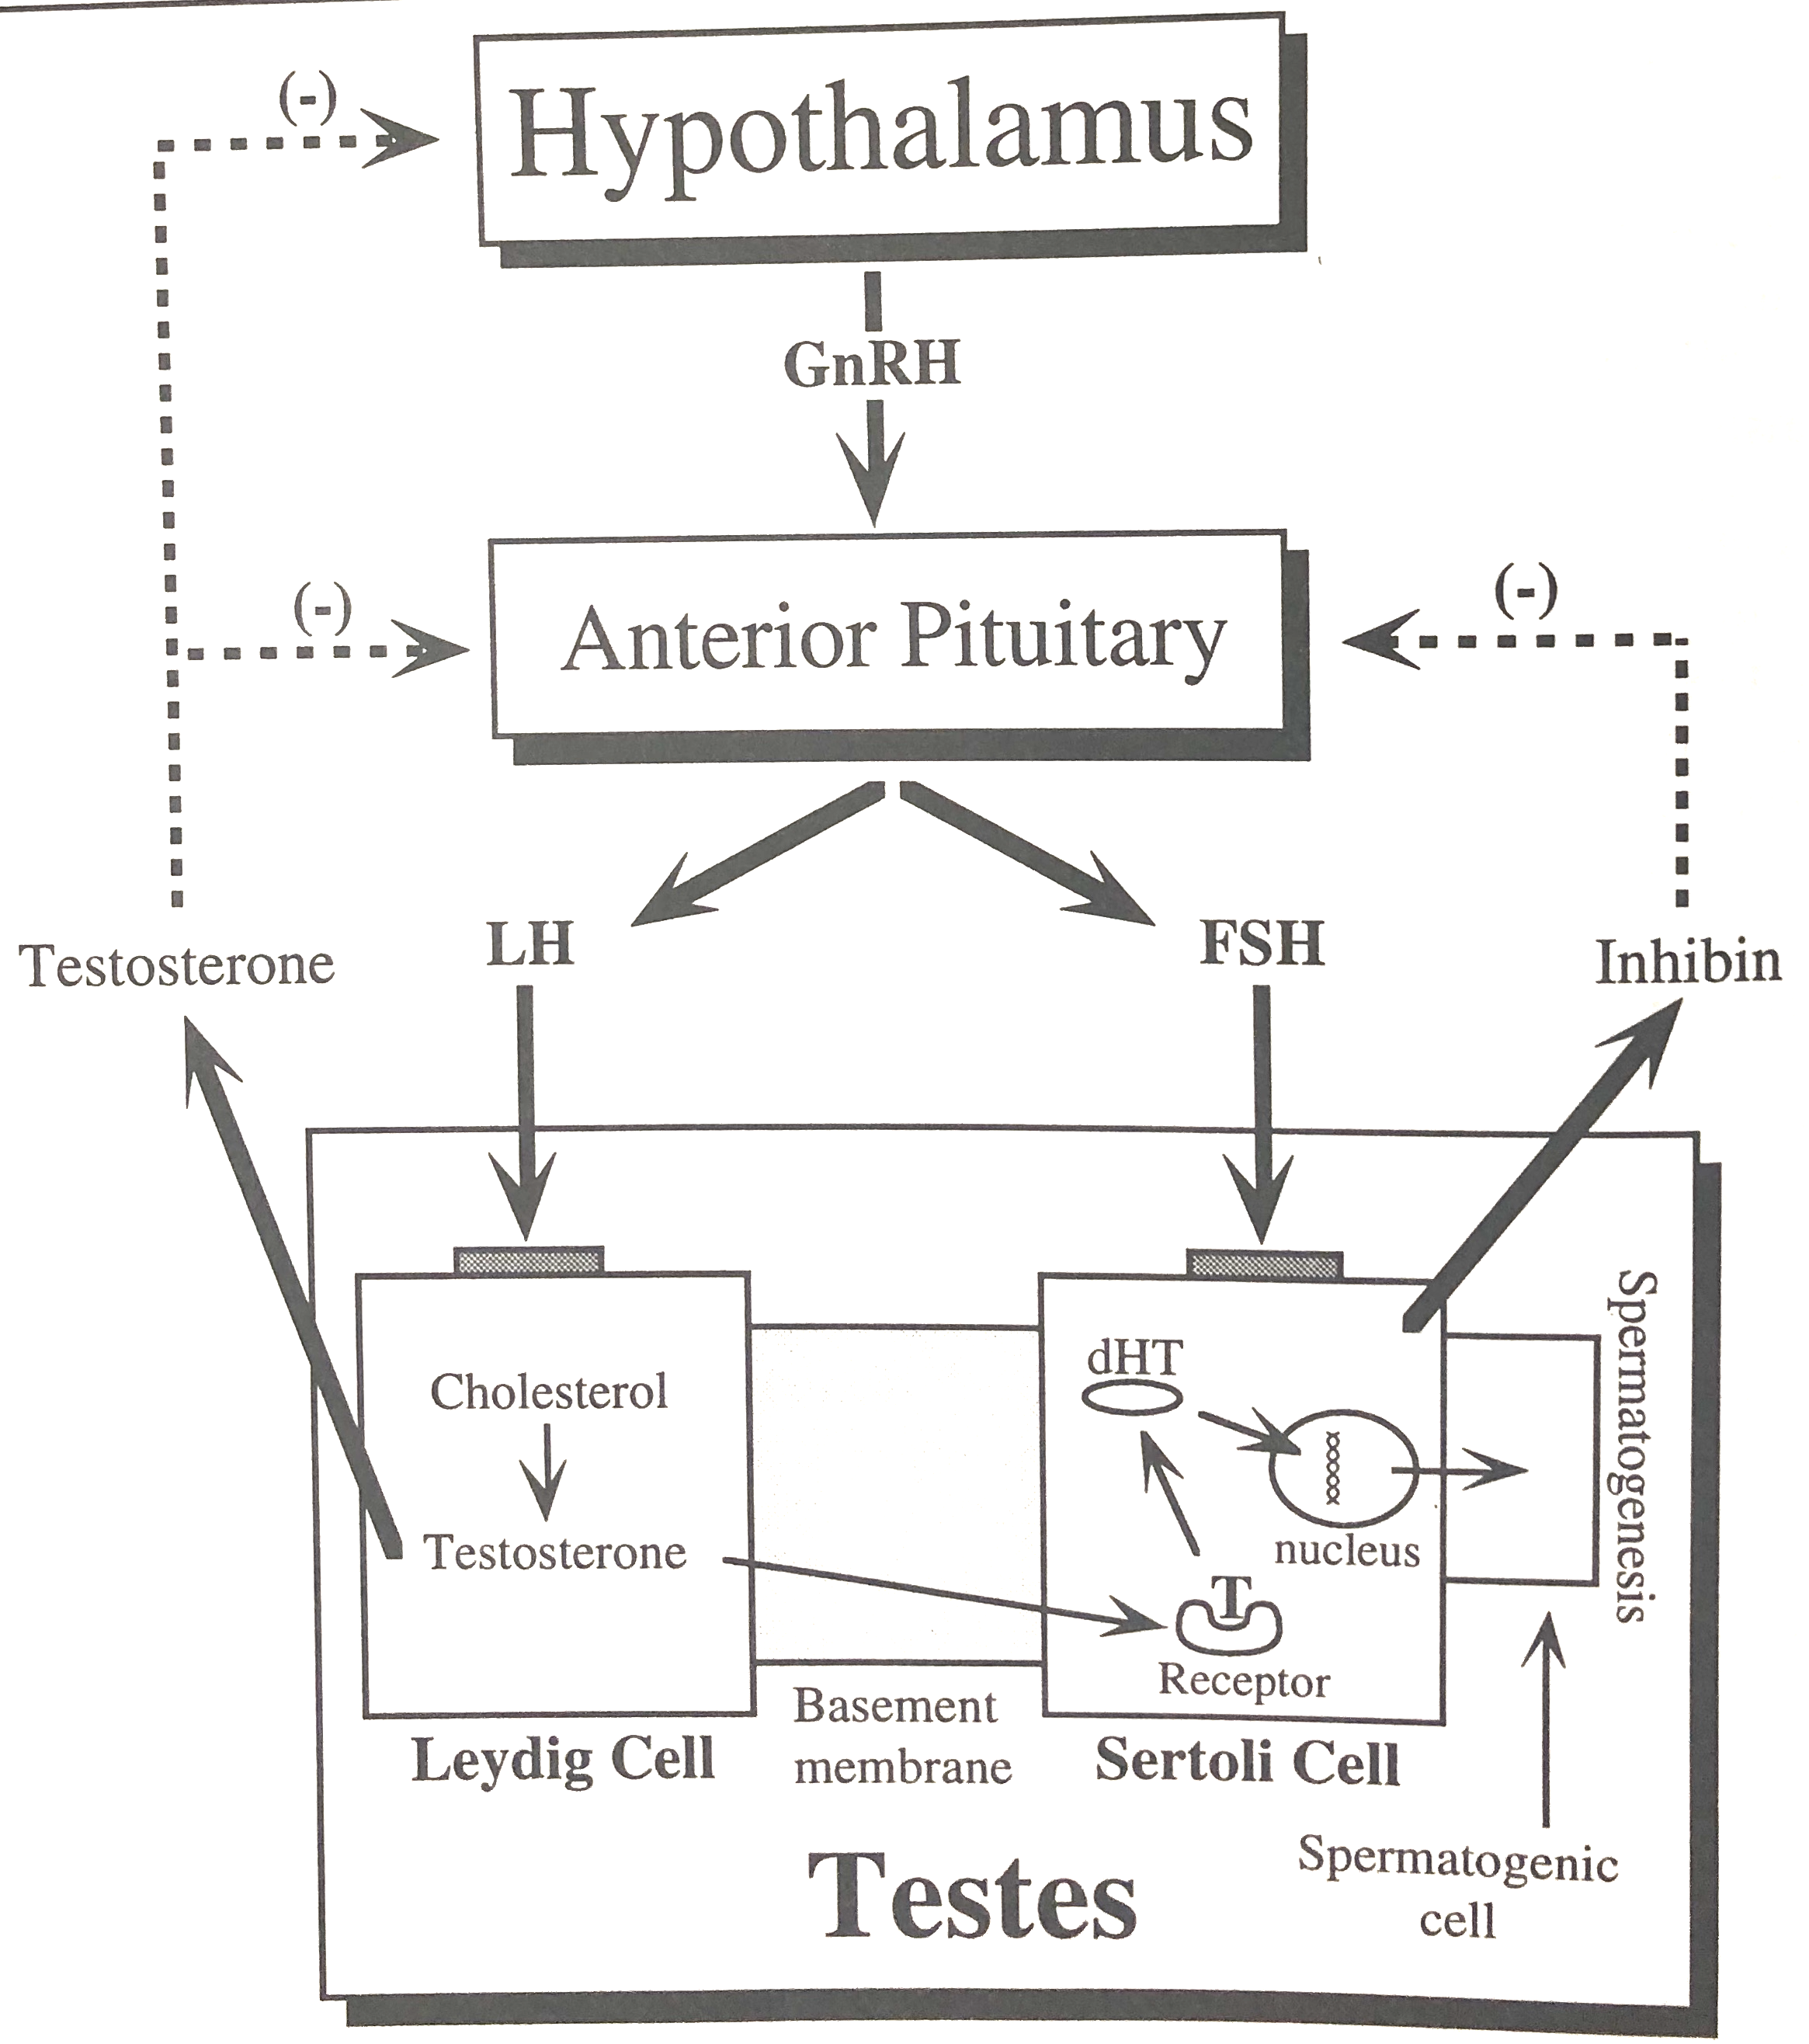
\includegraphics[width=0.5\textwidth]{testes_hormones.png} \label{testes_hormones}
\caption{Hormonal regulation in the testes.}
\end{figure}

\subsection{Female Reproduction}
Once sperm have been ejaculated into the vagina, they can live for about 48 hours. About half an hour after ejaculation, the leading sperm arrive at the \textbf{Fallopian tubes} (also called the \textbf{oviduct}), which is typically the site of fertilization. The fertilized egg continues to move down the oviduct towards the uterus, where it will implant in the uterine lining. About a week after ovulation the fertilized egg, now called a \textbf{blastocyst}, implants in the lining of the uterus where it will continue to grow and develop until \textbf{parturition} (delivery). The general female reproductive anatomy is shown in \textbf{Fig. \ref{female_reproductive_anatomy}}.
\begin{figure}[!ht]
\centering
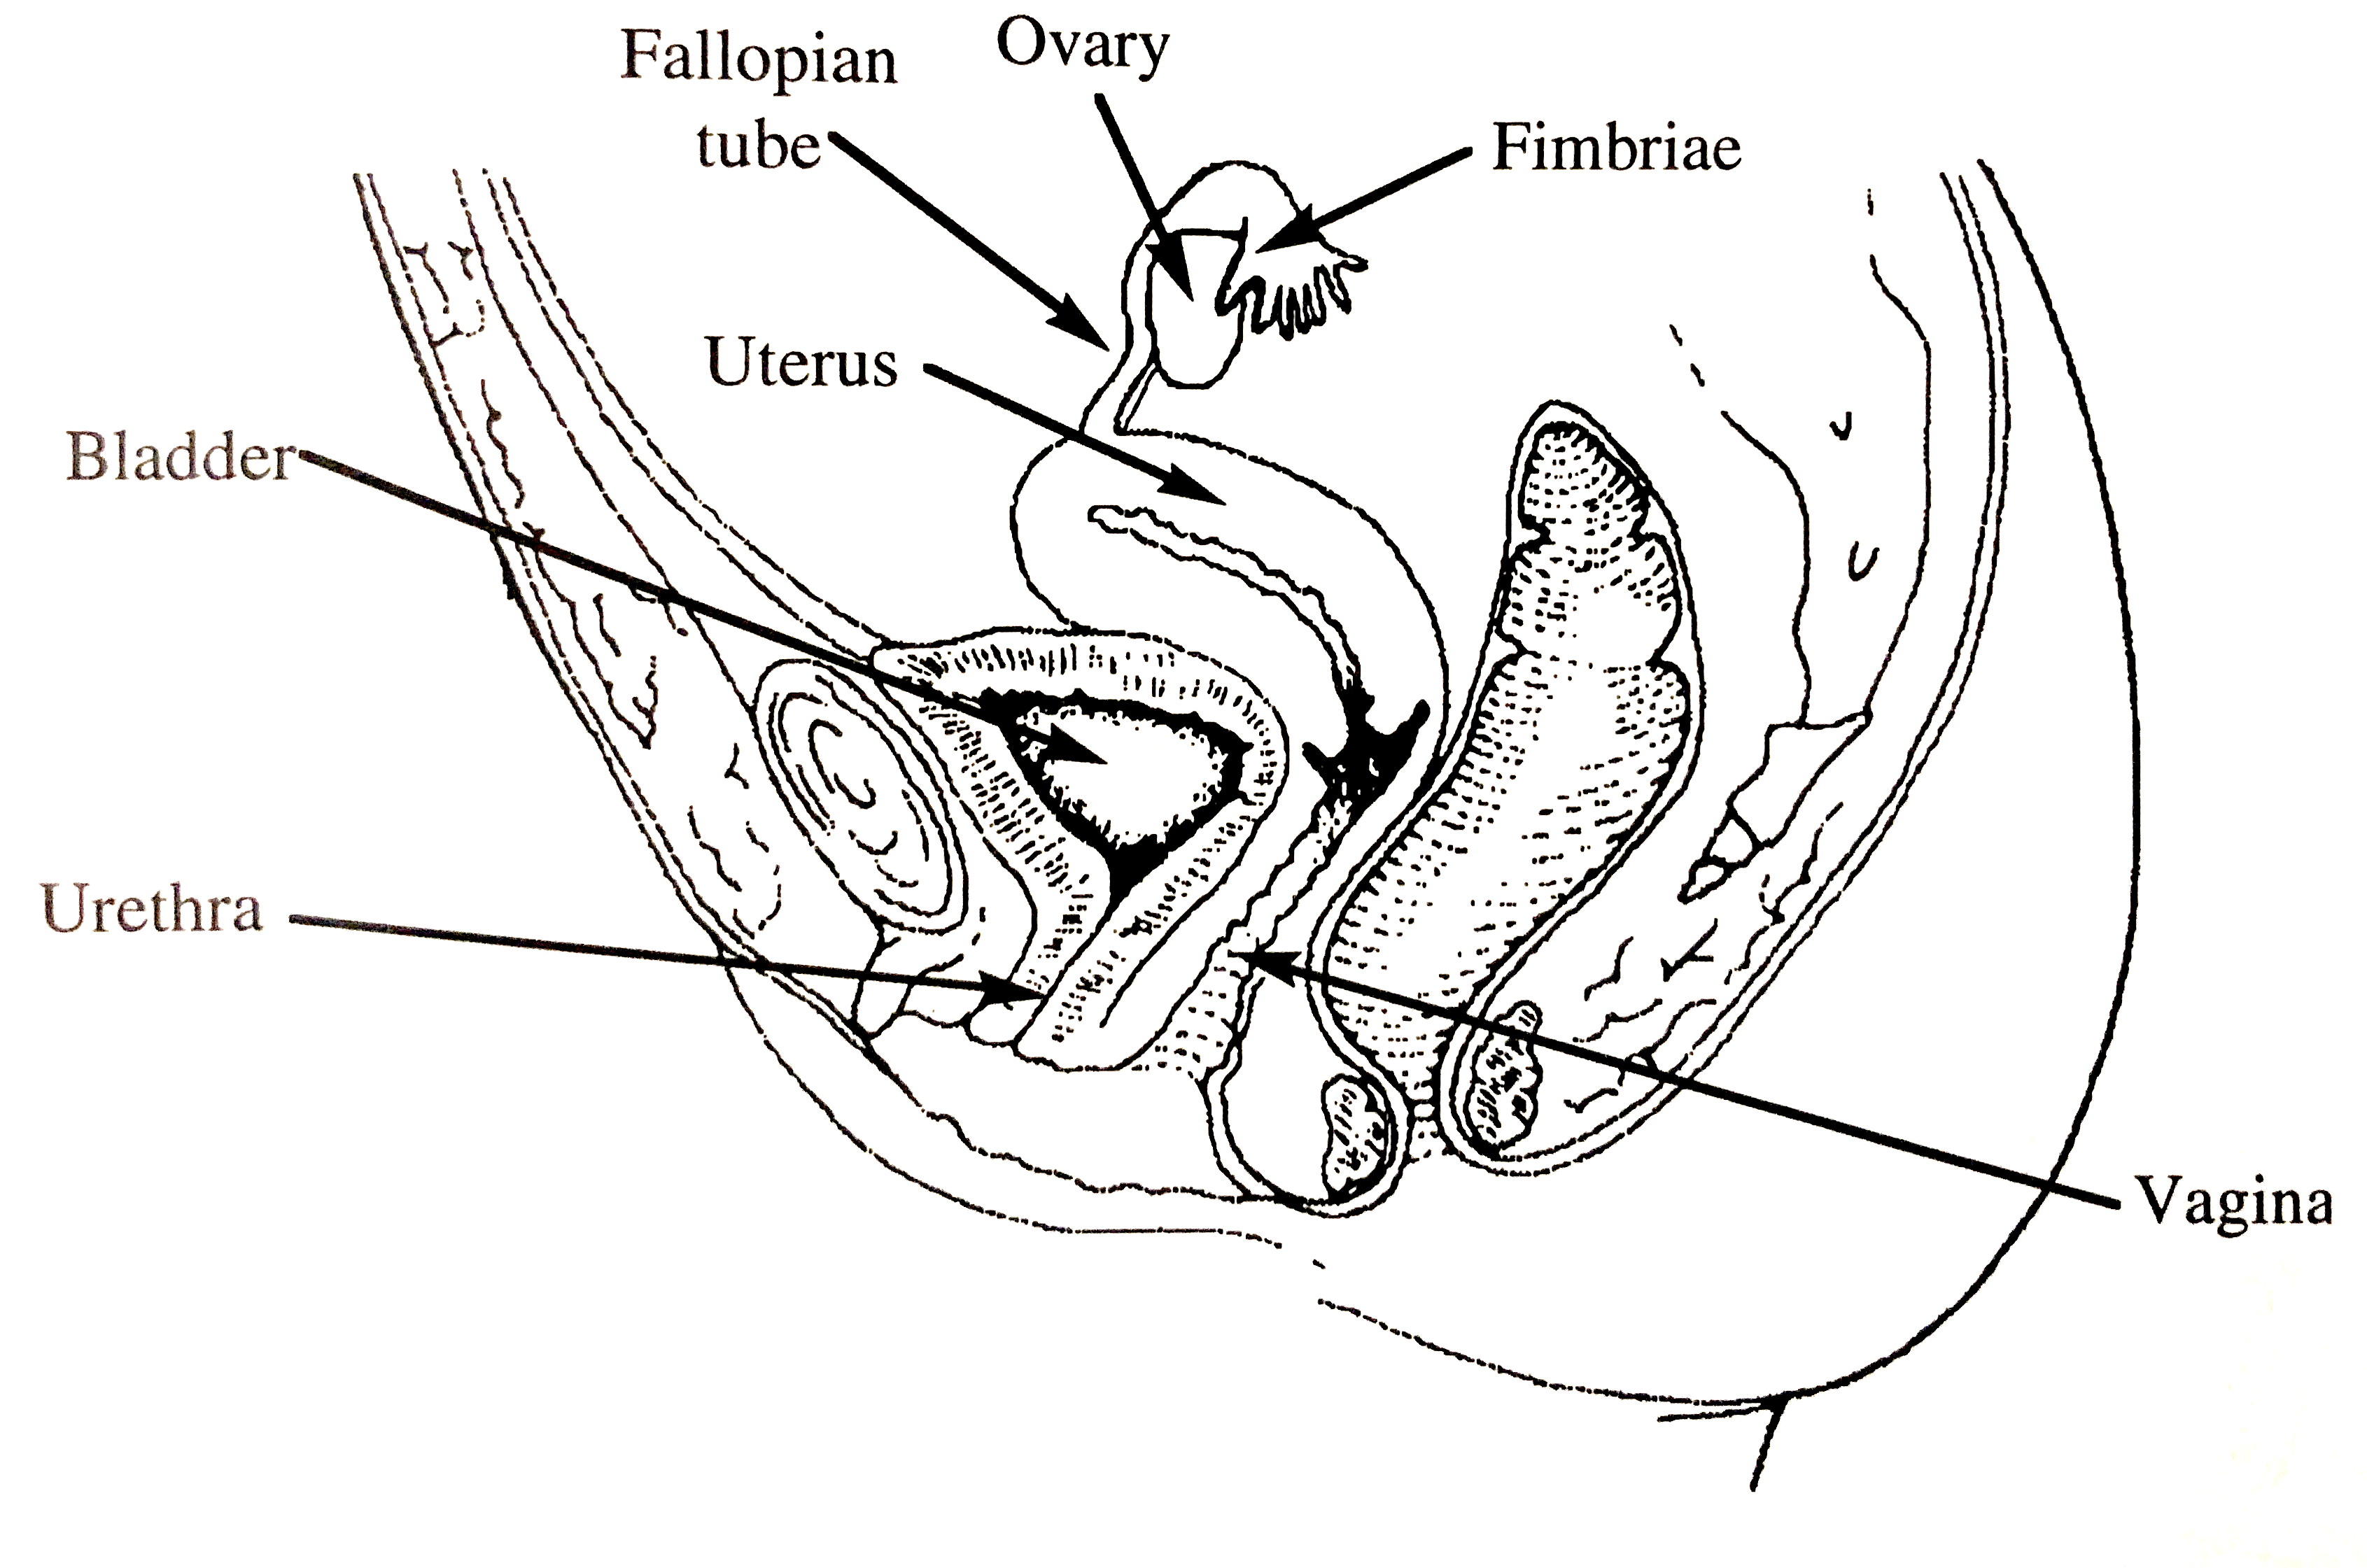
\includegraphics[width=0.7\textwidth]{female_reproductive_anatomy.png} \label{female_reproductive_anatomy}
\caption{Female reproductive anatomy.}
\end{figure}
\noindent The production of female germ cells is called \textbf{oogenesis}. First, oogonia mitotically divide to form \textbf{primary oocytes}. All of these divisions to form primary oocytes occur in the first \textit{two to three months of fetal development}. At birth a female will have about 400,000 primary oocytes, but by the time she has finished her reproductive life only about 400 will have ever matured. The remaining primary oocytes will have degenerated at various stages during the developmental process\textemdash the process of degeneration is called \textbf{atresia}.\\
\indent The primary oocytes then undergo the first meiotic division, caused by a surge in the gonadotropin \textbf{LH}, forming the \textbf{secondary oocytes}. This first meiotic division happens in monthly cycles. During this division, one of the two daughter cells obtains all the cytoplasm while the other is just a small sphere of DNA called the \textbf{first polar body}. The secondary oocyte undergoes the second meiotic division \textit{only after fertilization has taken place}. The result of that division is the \textbf{ovum} and a \textbf{second polar body}. The first polar body also divides to give two second polar bodies as well.\\
\indent If we take a cross-section of the ovary, we will see a series of specific cell types called \textbf{primary follicles} that are in different developmental states. The primary follicle is a \textbf{primary oocyte} surrounded by a layer of follicle cells. These follicle cells are in constant contact with the primary oocyte. Eventually, one of the primary follicles will start to develop (two of them if there are fraternal twins). In order to mature the primary oocyte, \textbf{estrogen}, \textbf{LH}, and \textbf{FSH} are needed. This developing time period is referred to as the \textbf{follicular phase} and lasts up to about the 14th day of the woman's monthly cycle. During this period, the primary follicle gradually develops. Surrounding the primary oocyte will be a membrane called the \textbf{zona pellucida}, which itself is surrounded by more follicle cells called \textbf{granulosa cells} and finally by \textbf{theca cells}. These cell types are a direct result of the estrogen, LH, and FSH that are present. The \textbf{theca cells} are analogous to the \textbf{Leydig cells} in the male, while the \textbf{granulosa cells} are analogous to the \textbf{Sertoli cells} in the male.\\
\indent Within the primary follicle, a fluid starts to build up forming the \textbf{antrum}. Next, the \textbf{LH surge} event causes the primary oocyte to undergo the first meiotic division, forming a polar body and secondary oocyte. The LH surge also causes the production of a series of enzymes that break down the membrane in the primary follicle. Once the secondary oocyte is released, \textbf{ovulation} has occurred. Ovulation usually comes at about the 14th day in the woman's monthly cycle. The left over follicle after the completion of the follicular phase is transformed into a gland-like structure called the \textbf{corpus luteum}. One of the main functions of the corpus luteum is to produce \textbf{estrogen} and \textbf{progesterone}. If fertilization does not occur and there is no pregnancy, the corpus luteum will degenerate and the whole cycle starts again. From the point of ovulation, at about the 14th day, until the beginning of the menstrual flow is the \textbf{luteal phase}. See \textbf{Fig. \ref{ovarian_cycle}}.\\
\begin{figure}[!ht]
\centering
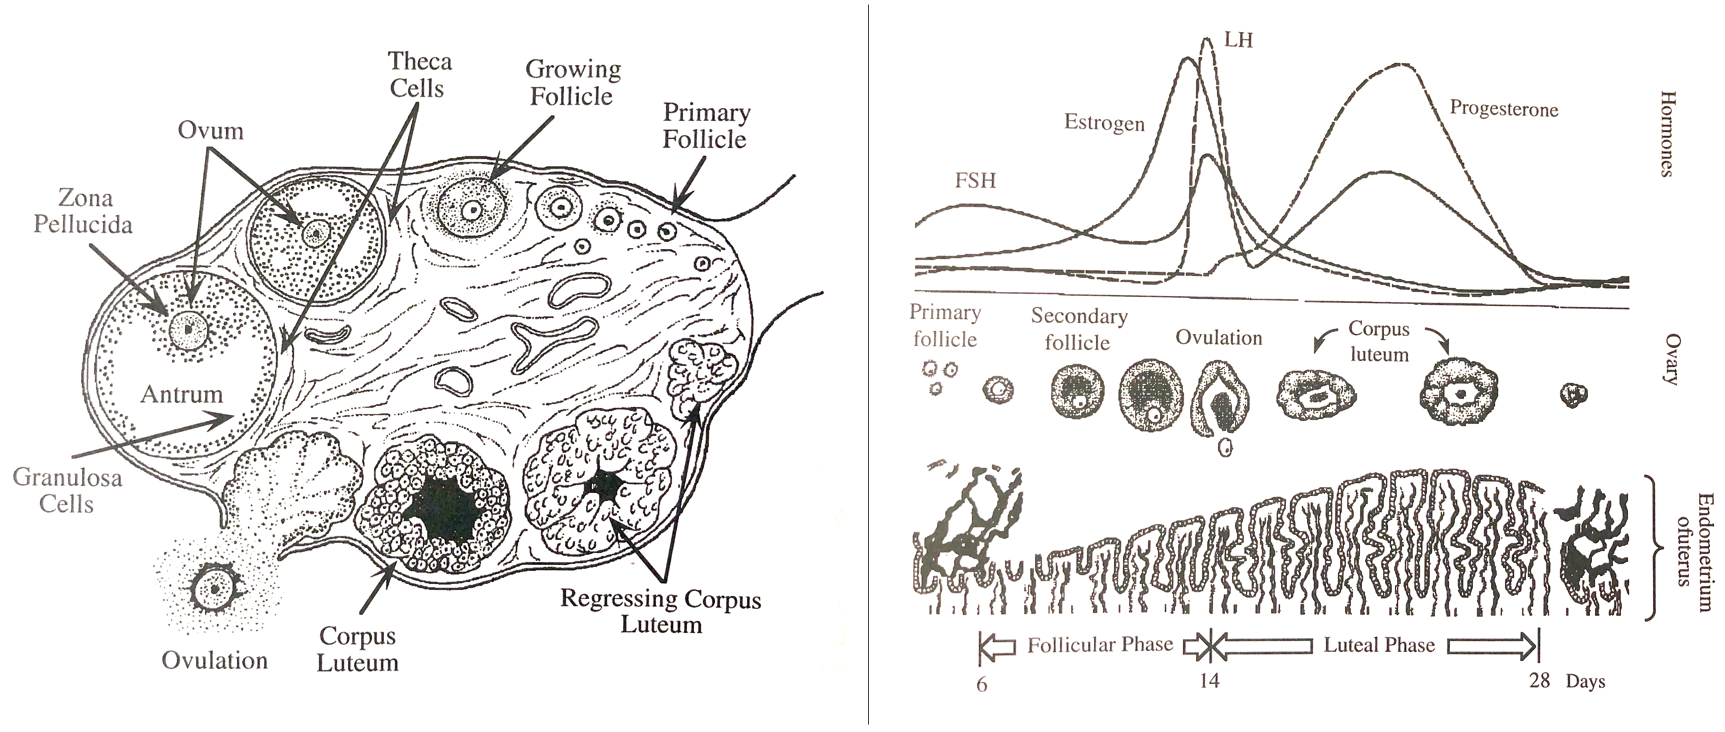
\includegraphics[width=\textwidth]{ovarian_cycle.png} \label{ovarian_cycle}
\caption{The ovarian cycle and its associated hormones.}
\end{figure}
\indent As we've mentioned previously, the \textbf{theca cells} convert cholesterol into \textbf{testosterone}, which diffuses into the follicle cells where it is converted into \textbf{estrogen}. Estrogen helps in the development of the primary follicle (i.e. the primary oocyte). Meanwhile, recall that the anterior pituitary secretes LH and FSH\textemdash LH affects the theca cells while FSH affects the follicle cells. As estrogen is being synthesized, the primary oocyte is developing so we have a proliferation of follicle cells. If we have more follicle cells, then we can synthesize more estrogen. This is where the first estrogen surge (the one in the follicular phase) comes from. It turns out that at low concentrations of estrogen there is a negative feedback on FSH production. However, as the follicle cells are growing, they reach a certain threshold level of estrogen where at these high concentrations, estrogen actually has a \textit{positive feedback} on the anterior pituitary and LH production. Thus, with a high level of estrogen production, we can now have the \textbf{LH surge}. \\
\indent Immediately following the LH surge, the levels of LH drop down to very low levels. This is because at ovulation the follicle cells become transformed into the \textbf{corpus luteum}, meaning they are no longer follicle cells and hence transiently lose their ability to produce estrogen. Since we no longer have the high concentration of estrogen, we lose the positive feedback on the anterior pituitary.\\
\indent Eventually, the corpus luteum becomes an endocrine gland and begins to synthesize estrogen and progesterone. Together, these hormones have a negative feedback on LH and FSH production in the anterior pituitary, and also on the hypothalamus on GnRH synthesis. Essentially, this prevents the primary follicle from developing, which is good because at this point there's no reason to have another primary follicle made. Remember, estrogen (in high concentrations) has a positive feedback, while estrogen and progesterone in the combination have a negative feedback. \\
\indent During pregnancy, things are a bit different. The acrosome of the spermatozoan allows for the digestion of the membrane of the secondary oocyte. After the nucleus of the sperm enteres the secondary oocyte, the \textbf{zona pellucida} changes and prevents any other spermatozoa from entering\textemdash this process is referred to as \textbf{fertilization}. At this point the secondary oocyte undergoes the second meiotic division to form the \textbf{ovum} and the polar body. The nucleus of the sperm and egg fuse to form the \textbf{zygote}, which now has 46 chromosomes. The zygote rapidly develops and in about 7 days attaches itself as a \textbf{blastocyst} to the \textbf{uterine lining}. When the implantation takes place the \textbf{placenta}, made up of maternal and fetal cell types, begins to form.\\
\indent For obvious reasons, we don't want the development of another primary follicle during pregnancy. Thus, throughout pregnancy, there are high levels of estrogen and progesterone. These high levels are maintained during the last six months of pregnancy, but for different reasons as we will discover. 
\begin{enumerate}
	\item During the first three months, the corpus luteum is still a viable gland and secretes estrogen and progesterone. The placenta is also an endocrine gland and synthesizes \textbf{chorionic gonadotropin (CG)}, which stimulates the corpus luteum to make estrogen and progesterone. CG is only made during the first three months of pregnancy. During this time, estrogen and progesterone work together to prevent the formation of primary follicles (and hence ovulation and menstruation as well) during pregnancy. The \textbf{mammary gland} is also sensitive to certain hormones during this time, such as \textbf{prolactin} that comes from the anterior pituitary and acts in a positive feedback manner on the mammary gland, and also \textbf{chorionic somatomammotropin (CS)} which comes from the placenta. CS and prolactin basically help the mammary gland grow. Estrogen and progesterone has positive feedback on the mammary glands as well. 
	\item During the last six months of pregnancy, CG is no longer made, so there is a loss of feedback to the corpus luteum. After three months, the corpus luteum breaks down and the supply of estrogen and progesterone from it comes to a halt. However, at this point in time the placenta itself starts to synthesize estrogen and progesterone.
\end{enumerate}

\subsection{Development}
The \textbf{coelom} is the body cavity, basically the thoracic cavity and abdominal cavity. After fertilization, we have \textbf{cleavage} of the zygote, where the zygote rapidly diveds into many smaller cells without an overall increase in size. \textbf{Gastrulation} then follows, where the cells of the zygote move to form the three primary germ layers (ectoderm, mesoderm, and endoderm) of the organism. The next developmental stage is \textbf{neurulation}, where we begin to see the formation of the nervous system, the first organ system to begin differentiation. \textbf{Neural crest} formation is the fifth developmental stage, which helps to form parts of the nervous system, skull, and sensory organs. The last stage of development is \textbf{organogenesis}.
\begin{equation}
\begin{split}
\text{Fertilization}\rightarrow\text{Cleavage}\rightarrow\text{Gastrulation}\rightarrow\text{Neurulation}\rightarrow\text{Neural Crest Formation}\rightarrow\text{Organogenesis}
\end{split}
\end{equation}
\noindent Let's take a look at development in the frog to see an example of vertebrate development. In the unfertilized egg there is a large amount of yolk that resides in the \textbf{vegetal pole} (i.e. the lower hemisphere), which will act as food for the developing embryo. The \textbf{animal pole} (i.e. the upper hermisphere) contains mainly cytoplasm. The \textbf{gray crescent} is located on the \textbf{dorsal aspect} (i.e. the future back) of the egg, opposite to where the sperm penetrates the egg's membrane. It eventually is where we will find the spinal cord and brain. \\
\indent Once the zygote has formed, it undergoes special cell division to increase its mass but not its overall size. The individual cells involved in this growth are called \textbf{blastomeres}. Eventually, a small, solid ball of cells will be formed called a \textbf{morula}. Further cellular division results in the formation of a hollow ball of cells called the \textbf{blastula}, which includes a fluid-filled cavity called the \textbf{blastocoel}. These different initial stages are shown in \textbf{Fig. \ref{embryonic_development}}.\\
\begin{figure}[!ht]
\centering
\includegraphics[width=\textwidth]{embryonic_development.png} \label{embryonic_development}
\caption{Different stages in embryonic development.}
\end{figure}
\indent During \textbf{gastrulation}, rearrangement of cells occurs. Not far from the gray crescent, an opening develops in the blastula called the \textbf{blastopore}. Cells from the animal pole begin to migrate inwards through the \textbf{dorsal lip} of the blastopore. As this outer layer of cells migrates inward, they form a second layer of cells immediately below. The blastocoel is reduced in size and is ultimately eliminated\textemdash in its place, a new cavity is formed called the \textbf{archenteron}. At this stage, the embryo is referred to as a \textbf{gastrula}. Invagination of the outer cell layer produce two cell layers: the \textbf{ectoderm} (outer layer) and \textbf{endoderm} (inner layer). A layer of \textbf{mesoderm} will later form between these two cell layers. The different stages of gastrulation are shown in \textbf{Fig. \ref{gastrulation}}. In general, it seems that the generation of three cell layers has been conserved through the evolutionary process.\\
\begin{figure}[!ht]
\centering
\includegraphics[width=0.75\textwidth]{gastrulation.png} \label{gastrulation}
\caption{The process of gastrulation.}
\end{figure}
\indent Here are important \textit{developmental fates} to remember:
\begin{enumerate}
	\item \textbf{Endoderm:} inner lining of the digestive and respiratory tracts, and major glands of the body like the liver and pancreas.
	\item \textbf{Mesoderm:} notochord, heart, skeleton, muscle, outer coverings of internal organs, and reproductive organs.
	\item \textbf{Ectoderm:} skin, lens of the eye, brain and nervous system.
\end{enumerate}
\noindent These are just a few of the developmental fates of these cell layers. Now, during the next stage of development, \textbf{neurulation}, the ectoderm, mesoderm, and endoderm begin to form the structures that will eventually define the embryo and later the adult. Notably, the formation of the \textbf{notochord} takes place along the body midline, and is derived from the \textit{mesoderm}. Superior to the notochord is a mass of \textit{ectodermal cells} called the \textbf{neural plate}, which begins to fold in on itself and form the \textbf{neural groove}. As the neural groove forms, the mesoderm is also split and forms the coelom (i.e. the body cavity). The neural groove goes on to form the \textbf{neural tube}, which will eventually encase the spinal cord (encased in the \textit{spinal column}), and anterior to the spinal cord will form the brain. In other words, the neural plate, which is composed of ectodermal cells, gives rise to the nervous system. This tissue is referred to as \textbf{primordium}, and the embryo is referred to as a \textbf{neurula} during this stage of development. \textbf{Fig. \ref{neurulation}} shows the formation of the neural tube during neurulation.\\
\begin{figure}[!ht]
\centering
\includegraphics[width=0.75\textwidth]{neurulation.png} \label{neurulation}
\caption{Neural tube formation.}
\end{figure}\indent When the edges of the neural groove fused together and become the neural tube, specialized ectodermal cells were left outside the tube and are called \textbf{neural crest cells}. These cells begin to form various parts of the body, such as the sensory cells of the head, the adrenal medulla, and other things. This process is called \textbf{neural crest formation}.\\
\indent \textbf{Organogenesis} first begins with interactions between the ectoderm and mesoderm. The neural tube becomes longer and thinner. Mesodermal cells migrate towards the neural tube and eventually form the vertebral column. The brain and optic vesicles begin to form. As the neural tube continues to form, segments of mesodermal tissue called \textbf{somites} begin to appear, which eventually gives rise to the vertebrae, connective tissue, and muscles of the body.\\

\subsection{Developmental Mechanisms}
There are two general classes of interaction associated with the differentiation of cells that we need to consider: intracellular and intercellular interactions. Intracellular interactions usually result in the setting up of a \textit{prepattern}, while the intercellular interactions usually undergo \textit{developmental induction}. \\
\indent Recall that after fertilization and induction of development, the gray crescent forms at a point opposite to where the sperm penetrated the egg. The formation of the gray crescent is due to an intracellular interaction, and is not a prepatterned phenomenon simply because of the fact that the entry of the sperm in the animal half of the cell is random. However, once entry is made and the gray crescent forms, the dorsal midline is established. This allows us to define directions. In other words, prior to the first cellular division, the axes of the organism are already established. Hans Spemann showed that the gray crescent is essential for complete embryonic development in the 1920s.

\subsection{Human Embryo Development}
Recall that the \textbf{blastocyst} is a hollow ball of cells with a mass of cells on one side. The surrounding cells that form the ball are called the \textbf{trophoblast}, and the other are called the \textbf{inner cell mass}. If the lining of the uterus is prepared to receive the embryo, then it will implant. Otherwise, the embryo is rejected and sloughed off during the next menstrual period. After implantation, the trophoblastic cells grow into the lining of the uterus. (In fact, the cells of the trophoblast grow little finger-like projections into the uterus.)\\
\indent For nourishment, blood vessels from the umbilical cord grow into the projections of the trophoblast. There is a layer of cells between the trophoblast and the fetal blood vessels called the \textbf{chorion}, which preserves the barrier between the mother's and fetus's blood (but diffusion of nutrients and waste products may still occur). This whole exchange apparatus is called the \textbf{placenta}.\\
\indent The \textbf{inner mast cells} will undergo changes similar to those in the frog to form the three basic germ layers. We also have the \textbf{primitive streak}, which is equivalent to the neural plate in frogs, that forms in the ectoderm. Cells from the primitive streak migrate down between the ectoderm and endoderm to become the mesoderm. Further folding of the primitive streak gives rise to a neural groove and then a neural tube, etc. So, the formation of the primitive streak in mammals marks the beginning of gastrulation, which is quickly followed by neurulation. Cell fate determination from the three germ layers in humans is basically the same as in frogs.\\
\indent The embryo cannot implant if the uterus is not receptive\textemdash that is, if it is not \textbf{quiescent}. Furthermore, pregnancy will not be maintained by the uterus even after implantation unless it remains quiescent. So, to maintain the uterine lining through the first part of pregnancy, the trophoblastic cells secrete \textbf{chorionic gonadotropin (CG)}, which is a hormone that causes the corpus luteum to continue to produce estrogen and progesterone. Eventually, the placenta can take over the production of estrogen and progesterone itself and the corpus luteum is no longer needed.\\
\indent The placenta secretes increasing amounts of estrogen and progesterone, but the levels of estrogen increase faster than those of progesterone. At some point near the end of pregnancy, the levels of progesterone plateau, and at a critical ratio of [estrogen]:[progesterone], the uterus is no longer quiescent; it begins to have contractions. The smooth muscle of the uterus contracts, putting the walls of the uterus under tension that thus sends nerve impulses to the hypothalamus. The hypothalamus then sends signals to the posterior pituitary to release \textbf{oxytocin}, which is a strong inducer of more contractions of the smooth muscle of the uterus. Oxytocin also stimulates the production and secretion of prostaglandins that further induce contractions. All of these hormones and nerves form a \textit{positive feedback system}. We call the birth process \textbf{parturition}. \\
\indent Milk production and milk ejection are two important processes in lactation. There are epithelial cells within the breast that make up the glands that produce the milk, and around these cells, we have the myoepithelial cells that can contract around the milk glands, ejecting the milk. Production of milk is stimulated by the suckling of the infant on the mother's nipple. The nipple sends a nervous impulse to the hypothalamus, which responds by releasing \textbf{PRH (prolactin releasing hormone)}, which acts on the anterior pituitary. PRH stimulates the anterior pituitary to release \textbf{prolactin}, which goes into the bloodstream and stimulates the epithelial cells in the breasts which comprise the milk glands to produce more milk. Suckling on the nipple also tells the hypothalamus to send a nervous signal to the posterior pituitary and release \textbf{oxytocin}, which causes contraction of the myoepithelial cells in the breast to squeeze the milk out.

\subsection{Endocrinology}
Hormones can generally be divided into \textit{peptide} hormones (e.g. insulin), \textit{amine} hormones (e.g. epinephrine or adrenaline, which are classified as \textbf{catecholamines}), and \textit{steroids} (e.g. progesterone and estrogen). \textit{Catecholamines} are monoamine neurotransmitters, which are organic compounds that have a catechol (benzene with two hydroxyl side groups next to each other) and a side-chain amine. Hormones are released by endocrine organs into the blood and travel by way of the circulatory system to various target tissues. To illustrate the importance of hormones, let's consider the action of the catecholamine epinephrine (adrenaline) on a typical hepatic (liver) cell. When the body is under some type of stress like physical exercise or even fright, an increased need for glucose arises.\\
\indent One a stress has been perceived, the nervous system responds by signaling the adrenal medulla (part of the adrenal gland that sits on top of the kidneys) to release epinephrine into the extracellular fluid. Epinephrine diffuses into the blood, and the \textbf{$\beta$-adrenergic receptors} on hepatic cells bind to epinephrine and cause the activation of \textbf{adenylate cyclase} (bound on the cytoplasmic membrane surface), which increases the concentration of cAMP (cyclic adenosine monophosphate, a second messenger) in the cell. $\beta$-adrenergic receptors are a type of \textit{G-protein coupled receptors}. GTP-bound state corresponds to the active state, while GDP-bound state corresponds to the inactive state. The increase in cAMP concentration allows cAMP to interact with \textit{protein kinase A} (PKA) and help it phosphorylate an enzyme called \textbf{\textit{glycogen phosphorylase}}. Once glycogen phosphorylase has become phosphorylated, it is now an active enzyme and catalyzes the conversion of glycogen into glucose.\\
\indent \textbf{Cholera} is an intestinal disorder caused by the \textit{Vibrio cholerae} bacterium. The major symptom of this disorder is \textbf{diarrhea}, and if left untreated will result in severe dehydration and eventual death. This toxin binds to the active state of the G protein and prevents GTP from being hydrolyzed to GDP. This means that the adenylate cyclase enzyme is continually active and massive amounts of cAMP are synthesized. cAMP causes the intestinal cells to secrete digestive fluids. \\
\indent Let's consider another example, this time involving the water-soluble peptide hormone \textbf{gastrin} that stimulates the secretion of HCl and pepsinogen from the stomach in response to stimulation from the vagus nerve and partially digested protein. Gastrin first binds to a GPCR, activating an associated G-protein that can now interact with the membrane enzyme \textbf{phospholipase C (PLC)}, and this interaction induces PLC to hydrolyze phosphatidyl-inositol-4,5-biphosphate (PIP\textsubscript{2}) to inositol-1,4,5-triphosphate (IP\textsubscript{3}) and 1,2-diacylglycerol (DAG). IP\textsubscript{3} is a second messenger that interacts with the IP\textsubscript{3}-sensitive calcium ion channels in the endoplasmic reticulum membrane, stimulating the release of \ce{Ca^{2+}} ions into the cytosol from the ER lumen. Meanwhile, DAG, diffusing through the plasma membrane, interacts with \textbf{protein kinase C} and stimulates that kinase with the help of \ce{Ca^{2+}} to phosphorylate an unknown protein which in turn causes HCl secretion into the lumen of the stomach. \\
\indent Another example of a peptide hormone in action involves insulin, which is a water-soluble peptide hormone that binds to a specific trans-membrane receptor in the cell membranes of liver, fat, and muscle cells. Once insulin binds to the receptor on the cell surface, the cytoplasmic portion of the receptor is converted into a tyrosine kinase that autophosphorylates the amino acid tyrosine found within the cytoplasmic portion of the receptor. This acts to further enhance the activity of the tyrosine kinase. Presumably, the insulin receptor can also internalize and somehow act as a second messenger. This action, along with enhanced tyrosine kinase activity, leads to the internalization of glucose into the cells. The actual events in the insulin signaling mechanism that leads to the uptake of glucose are somewhat obscure at the present time.\\
\indent While these show a lot about the some of the many different pathways in cell signaling, kind of the main thing to pay attention to is that peptide and catecholamine hormones always involve some signaling intermediates because they can't diffuse freely through the membrane. Contrast this with steroid and thyroid hormones, which are lipid soluble hormones that can pass through the cell's plasma membrane and interact with a receptor either in the cytosol or in the nucleus. \textbf{Thyroid hormones} can diffuse across the plasma membrane and into the nucleus where they ind with specific receptors. The hormone receptor complex then activates transcription essential for certain metabolic processes; indeed, thyroid hormones help to regulate growth and differentiation and they can stimulate the breakdown of proteins, fats, and glucose.\\
\indent There are four major types of regulatory mechanisms in endocrinology: endocrine, neuroendocrine, paracrine, and autocrine. We go over an example of each here: 
\begin{itemize}
	\item \textbf{Endocrine Regulation:} The \textbf{pancreas} secretes insulin and glucagon, which are two hormones that are important in maintaining the proper levels of blood glucose. Both of these hormones are secreted from clusters of specialized cells called the \textbf{islets of Langerhans}. Insulin is secreted by the $\beta$ cells, while glucagon is secreted by the $\alpha$ cells. An increase in blood glucose stimulates the $\beta$ cells to produce insulin and excrete it into the blood, which goes to the liver, fat, and muscle cells and tells them to uptake glucose, thus decreasing blood glucose levels. Similarly, a decrease in blood glucose stimulates the $\alpha$ cells to produce glucagon and excrete it into the blood, which goes to the lever and fat cells and tells them to release glucose and fatty acids, thus increasing blood glucose levels. This is an example of \textbf{negative feedback}.
	\item \textbf{Neuroendocrine Regulation:} In this case, the hormone is not released for an endocrine cell, but rather from a nerve cell which releases its neurotransmitter in the form of a hormone into the blood. For example, the \textbf{adrenal medulla} can receive sensory input from a sympathetic nerve, which tells it to release epinephrine into the blood. Other examples of neuroendocrine regulation involve the \textbf{hypothalamus} and the \textbf{pituitary gland}. The pituitary gland can be divided into the \textbf{anterior} and \textbf{posterior pituitary}.
	\item \textbf{Paracrine Regulation:} In paracrine regulation, the chemical that acts as a signal is released from one cell and influences a cell immediately adjacent to it. An example of such a paracrine cell would be \textbf{mast cells}, which contain large amounts of \textbf{histamine}. The substances released by the paracrine cell are generally dumped into the extracellular space and not into the bloodstream. Other examples of a paracrine signal would be neurohormones and neurotransmitters.
	\item \textbf{Autocrine Regulation:} In autocrine regulation, cells can release certain chemicals which they can then respond to themselves. For example, certain cells can release growth factors which can then bind to specific receptors on the membrane of that same cell. Thus, the cells that released the growth hormone are stimulated to grow.
\end{itemize}

\subsection{The Pituitary Gland}
The posterior pituitary releases \textbf{oxytocin} and \textbf{antidiuretic hormone}, which are synthesized in specific cells of the hypothalamus. Oxytocin stimulates female uterine contraction in a positive feedback loop while antidiuretic hormone (ADH) stimulates water and \ce{Na^{2+}} reabsorption int he kidneys and also helps to increase the blood volume/pressure. The ADH that is synthesized in the nerve cell bodies in the hypothalamus are packaged into vesicles and transported down the axon to the terminal bouton in the posterior pituitary. A nerve impulse propagates down that same axon and causes the release of these hormones into a system of nearby capillaries. ADH helps prevent \textbf{diuresis}, which is the excessive loss of urine.\\
\indent The anterior pituitary secretes six major hormones: thyroid stimulating hormone (TSH), adrenocorticotropic hormone (ACTH), follicle stimulating hormone (FSH), luteinizing hormone (LH), growth hormone (GH), and prolactin (PRL). These hormones are regulated by a second set of hormones stored in the ypothalamic nerves. For example, the hypothalamus has nerve cells that contain thyrotropin releasing hormone (TRH). When this nerve is stimulated, it secretes TRH into a set of capillaries which extend into the anterior pituitary. TRH stimulates the synthesis and release of TSH, which in turn binds to specialized receptors in the thyroid gland and causes the release of thyroxine. Thyroxine increases the rate of metabolism and growth as a part of a negative feedback loop.

\subsection{Immunology}
Blood contains \textbf{erythrocytes} (red blood cells), \textbf{leukocytes} (white blood cells), and platelets. Erythrocytes are produced in the marrow of the sternum, ribs, and vertebrae, while leukocytes are produced partially in the tissues of the lymph and partly in the bone marrow.\\
\indent There are six types of leukocytes found in the blood, but we are only interested in three of them: \textbf{monocytes}, \textbf{neutrophils}, and \textbf{lymphocytes}. Monocytes and neutrophils are considered to be \textbf{phagocytes}, which, along with \textbf{mast cells} and a variety of other cell types, participate in the \textit{immune response}. 
\begin{itemize}
	\item \textbf{Mast cells} are derived from leukocytes and then migrate out into the tissues where they reside. When mast cells are stimulated, they release \textbf{histamine} which acts on endothelial cells and causes an increased permeability to cells like neutrophils, allowing neutrophils easy access to the surrounding tissue in order to defend against foreign pathogens.
	\item \textbf{Phagocytes} include monocytes (i.e. \textbf{macrophages} when they leave the blood and enter into the tissues) and neutrophils. These cells are the primary cell types that attack and destroy foreign bacteria and viruses. They do this by the process of \textbf{phagocytosis}, engulfing the foreign invader by \textbf{endocytosis}. 
	\item \text{Lymphocytes} are derived from either the \textbf{thymus} gland (which produces \textbf{T lymphocytes}) or elsewhere from places that produce \textbf{B lymphocytes}. T cells are responsible for \textit{cell-mediated immunity}. These cells are responsible for the destruction of foreign microorganisms and other harmful agents. There are three types of T cells: cytotoxic/killer T cells, helper T cells, and suppressor T cells. B cells are responsible for \textit{humoral mediated immunity}. Upon infection, B cells can differentiate into \textbf{plasma cells} that can synthesize and secrete antibodies. \textbf{Antibodies} are proteins that are synthesized in response to an \textbf{antigen}, which is simply a foreign substance with high MW.
\end{itemize}
\noindent Let's go over the two types of general immune responses\textemdash cell-mediated immunity and humoral mediated immunity\textemdash in more detail:
\begin{itemize}
	\item \textbf{Cell-Mediated Immunity:} Macrophages engulfs a foreign particle and phagocytizes it. The antigenic fragments released into the cytosol of the macrophage are transported to the macrophage's membrane, where they bind to the \textbf{major histocompatibility complex protein, class 1 (MHCI)}. Certain receptors on \textbf{cytotoxic T cells} recognize the antigen-MHCI complex on the macrophage and bind to it, stimulating the release of growth factor \textbf{interleukin-1 (IL-1)} from the macrophage. The cytotoxic T cell also releases \textbf{interleukin-2 (IL-2)}. IL-1, IL-2, and other interleukins released by \textbf{helper T cells} (discussed below) stimulate the synthesis of more cytotoxic T cells. These killer T cells proliferate and bind to the invading foreign cells bearing the antigen, causing them to lyse.
	\item \textbf{Humoral Mediated Immunity:} B cells have \textbf{MHC class 2 (MHCII) proteins} and antibodies on their surface. When a B cell finds an antigen that has specifically bound to its antibody, it engulfs that antigen-antibody complex and transports a portion of that antigen to the MHCII protein, effectively `displaying' the complex on the surface of its membrane. \textbf{Helper T cells} with the right receptors are able to bind to the antigen-MHCII complexes, stimulating the helper T cells to release interleukins (a \textbf{lymphokine}). This stimulates the B cells to proliferate and form \textbf{plasma cells}, which in turn produce a vast amount of \textbf{antibodies} specific to the original antigen. When these circulating antibodies bind to the antigen, they act as a tag that signals circulating phagocytes to engulf the antigen-antibody complex and destroy it. The human immunodeficiency virus (HIV) acts at the level of the helper T cells by infecting them.
\end{itemize}

\subsection{Antibodies}
Most immunoglobulins (antibodies) are composed of 4 subunits arranged in a `Y' configuration. There are 2 light chains and 2 heavy chains. These subunits are joined to one another by disulfide bonds. Within each heavy and light chain are \textbf{variable domains} and \textbf{constant domains}. \\
\indent At the terminal ends of the heavy and light chains are variable (V) regions that can differ in amino acid sequence from immunoglobulin to immunoglobulin. The constant (C) regions of the heavy and light chains are found in the lower portions of the immunoglobulin. The \textbf{antigen binding site} for a particular antibody is located at the end of the variable regions of the heavy and light chains.\\
\indent Two other regions of the immunoglobulin are important: the diversity (D) and the joining (J) region. We show a picture of the general antibody structure in \textbf{Figure \ref{antibody_structure}}.
\begin{figure}[!ht]
\centering
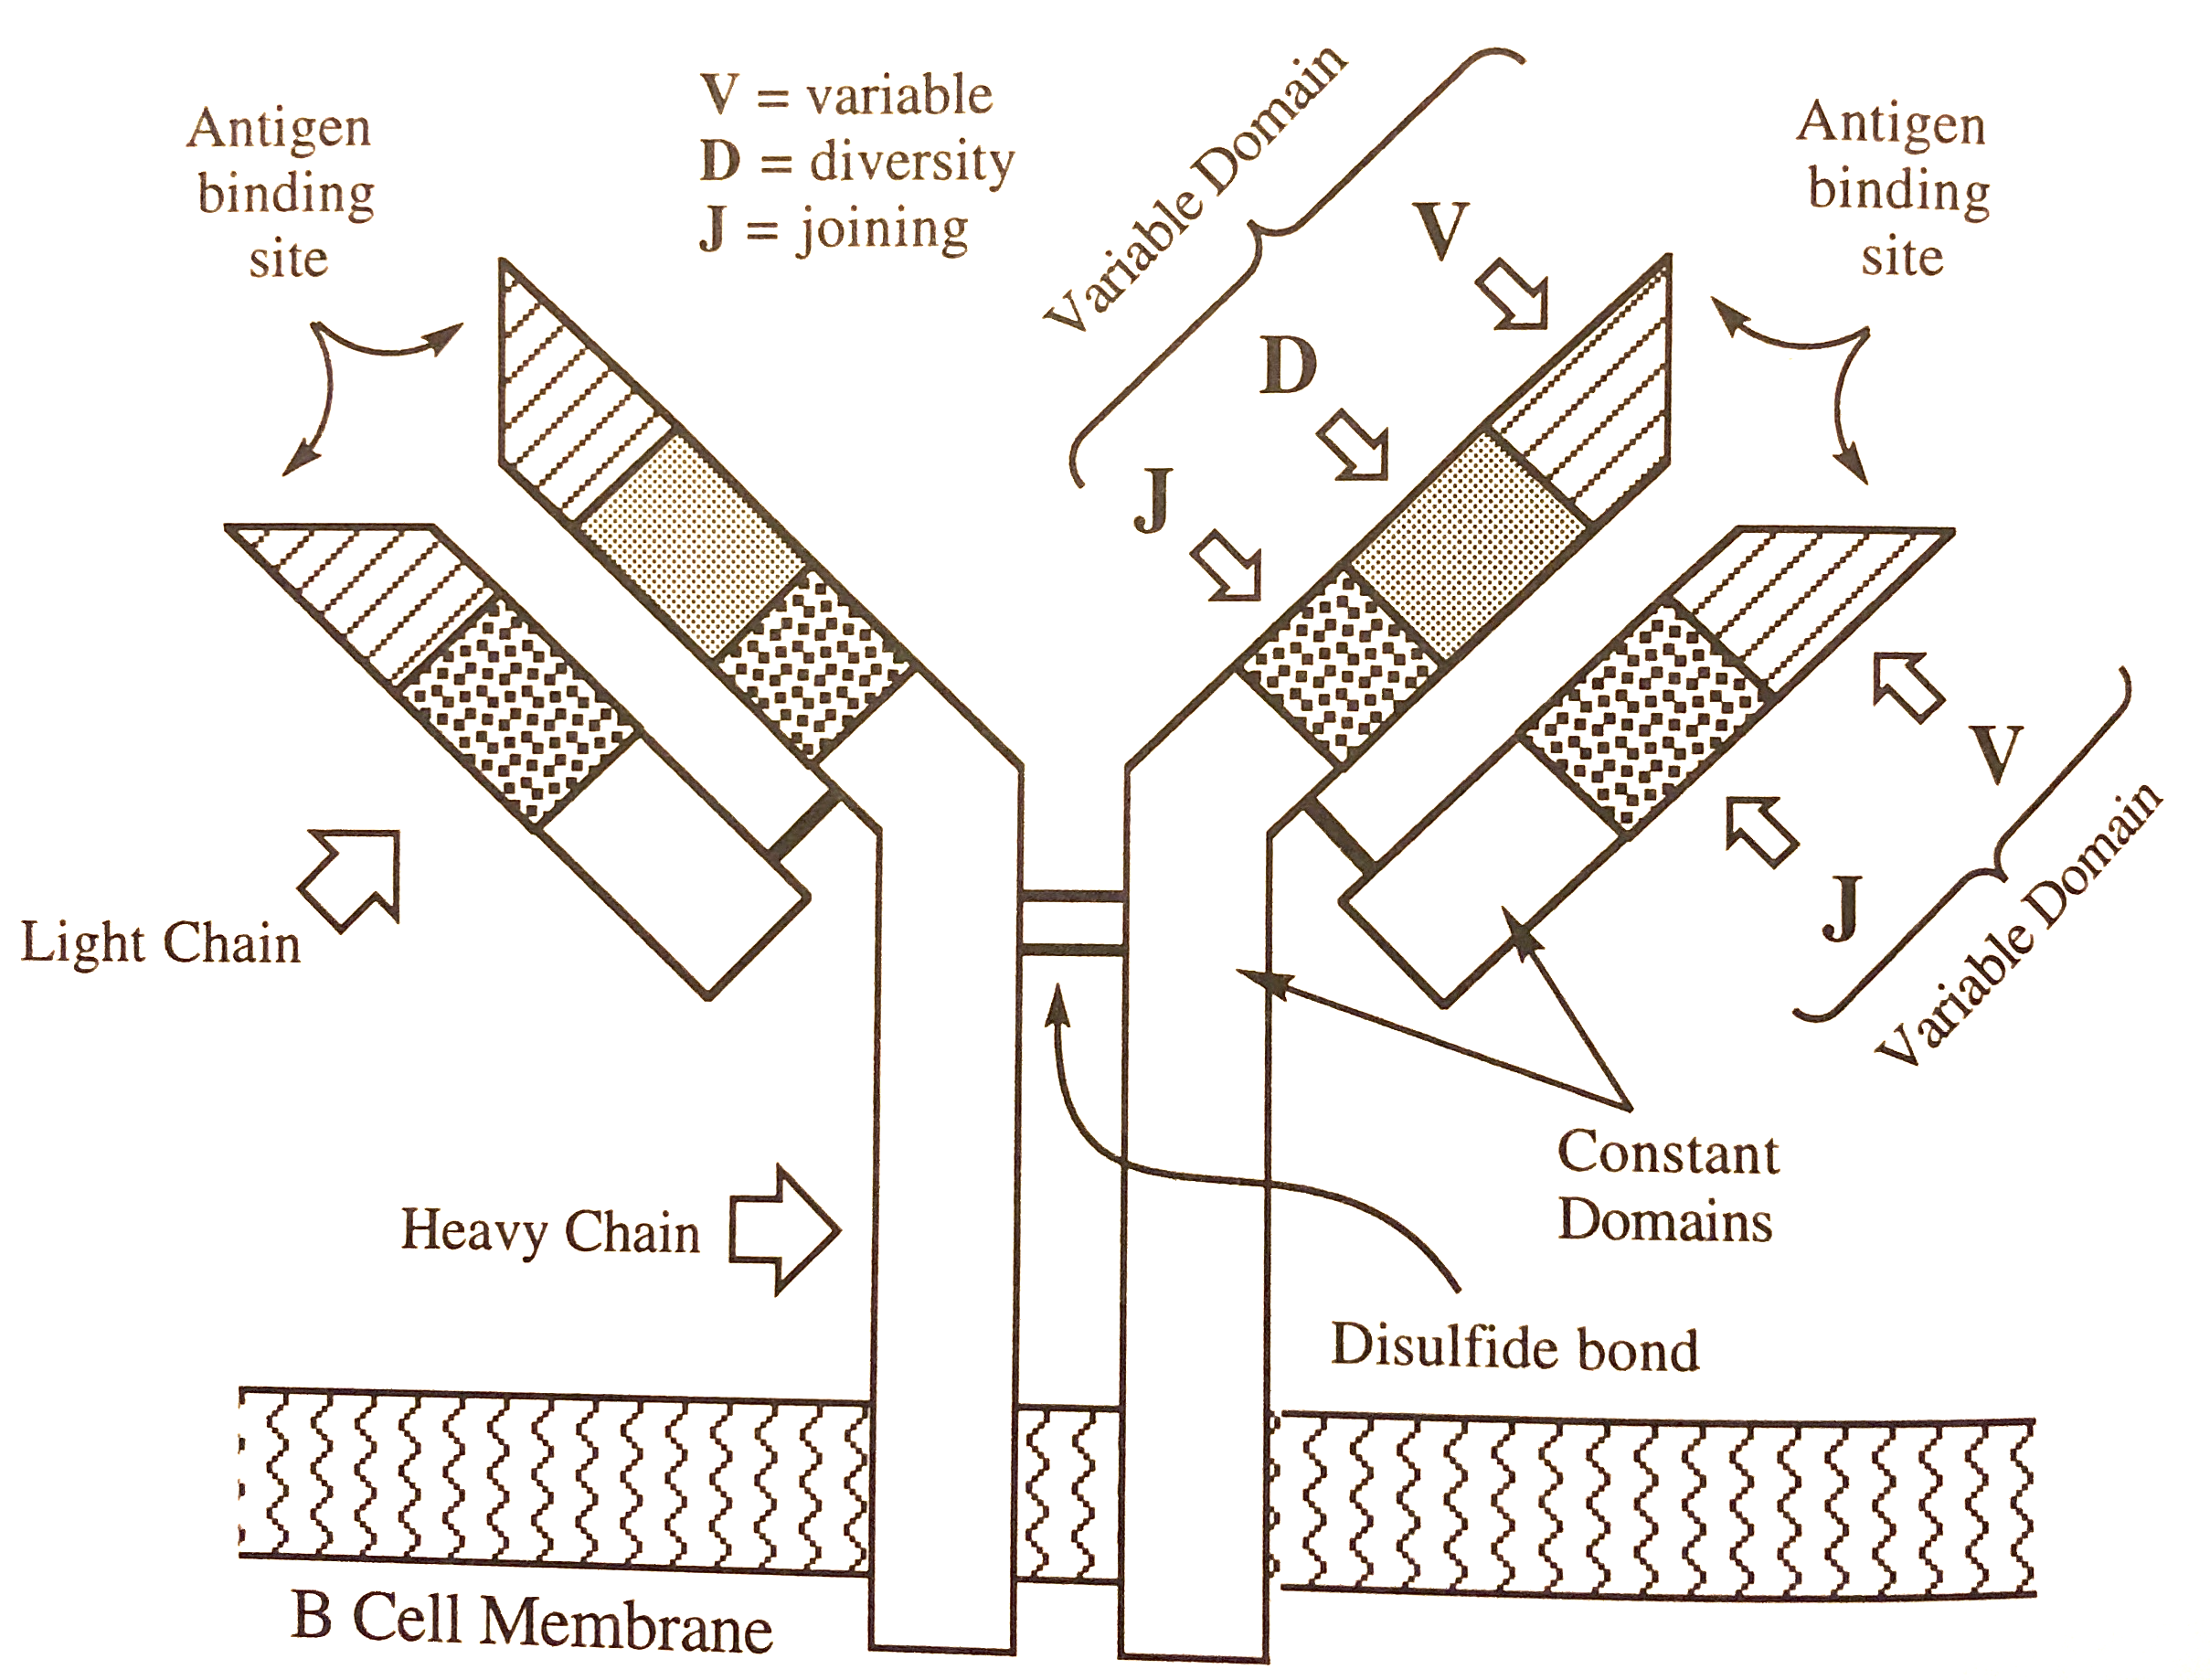
\includegraphics[width=0.7\textwidth]{antibody_structure.png} \label{antibody_structure}
\caption{Generalized antibody structure.}
\end{figure}
\noindent There are five classes of immunoglobulins that differ in the composition of their heavy chains:
\begin{itemize}
	\item \textbf{IgA:} Found in milk and helps to protect nursing infants.
	\item \textbf{IgD:} Has unknown function.
	\item \textbf{IgE:} Binds to mast cells and is involved in the allergic reaction.
	\item \textbf{IgG:} The only antibody able to cross the placenta. It is also the most abundant and is produced within days after the IgM antibody is secreted.
	\item \textbf{IgM:} Produced a few days after detection of an antigen and it is the first antibody produced in response to an antigen.
\end{itemize}
\noindent Antibodies simply recognize and identify foreign antigens, and can have different mechanisms by which to accomplish this function:
\begin{itemize}
	\item \textbf{Direct Blocking:} The antibody directly blocks the foreign invader from gaining access to host cells. This is accomplished by the antibodies binding to the antigens or other parts of the pathogen.
	\item \textbf{Complement:} An antibody has already recognized and bound to a specific antigen on a bacterial cell that is considered an intruder, and a complement protein (plasma protein) this antigen-antibody complex and binds to the Fc domain of the antibody. After a series of reactions, the complement protein is activated and triggers an immune response. Further reactions form a \textbf{membrane attack complex (MAC)} that inserts into the bacterial cell's membrane and forms a channel that lets water into the cell, causing it to swell with water and eventually lyse.
	\item \textbf{Coating the Cell Surface:} Antibodies can bind to specific antigens on the surface of a bacterial cell and coat the cell surface. Once the antibodies have attached to the bacterial cell, phagocytes and/or killer T cells can bind to the terminal portion of the Fc domain of the antibodies and begin to engulf the foreign invader.
\end{itemize}

\subsection{T Cells}
The receptors for T cells are composed of two polypeptide chains, each with a constant and variable domain. Within a variable domain in each polypeptide we find a variable (V) region and a joining (J) region. On one of the polypeptide chains is a diversity (D) region. 
\begin{figure}[!ht]
\centering
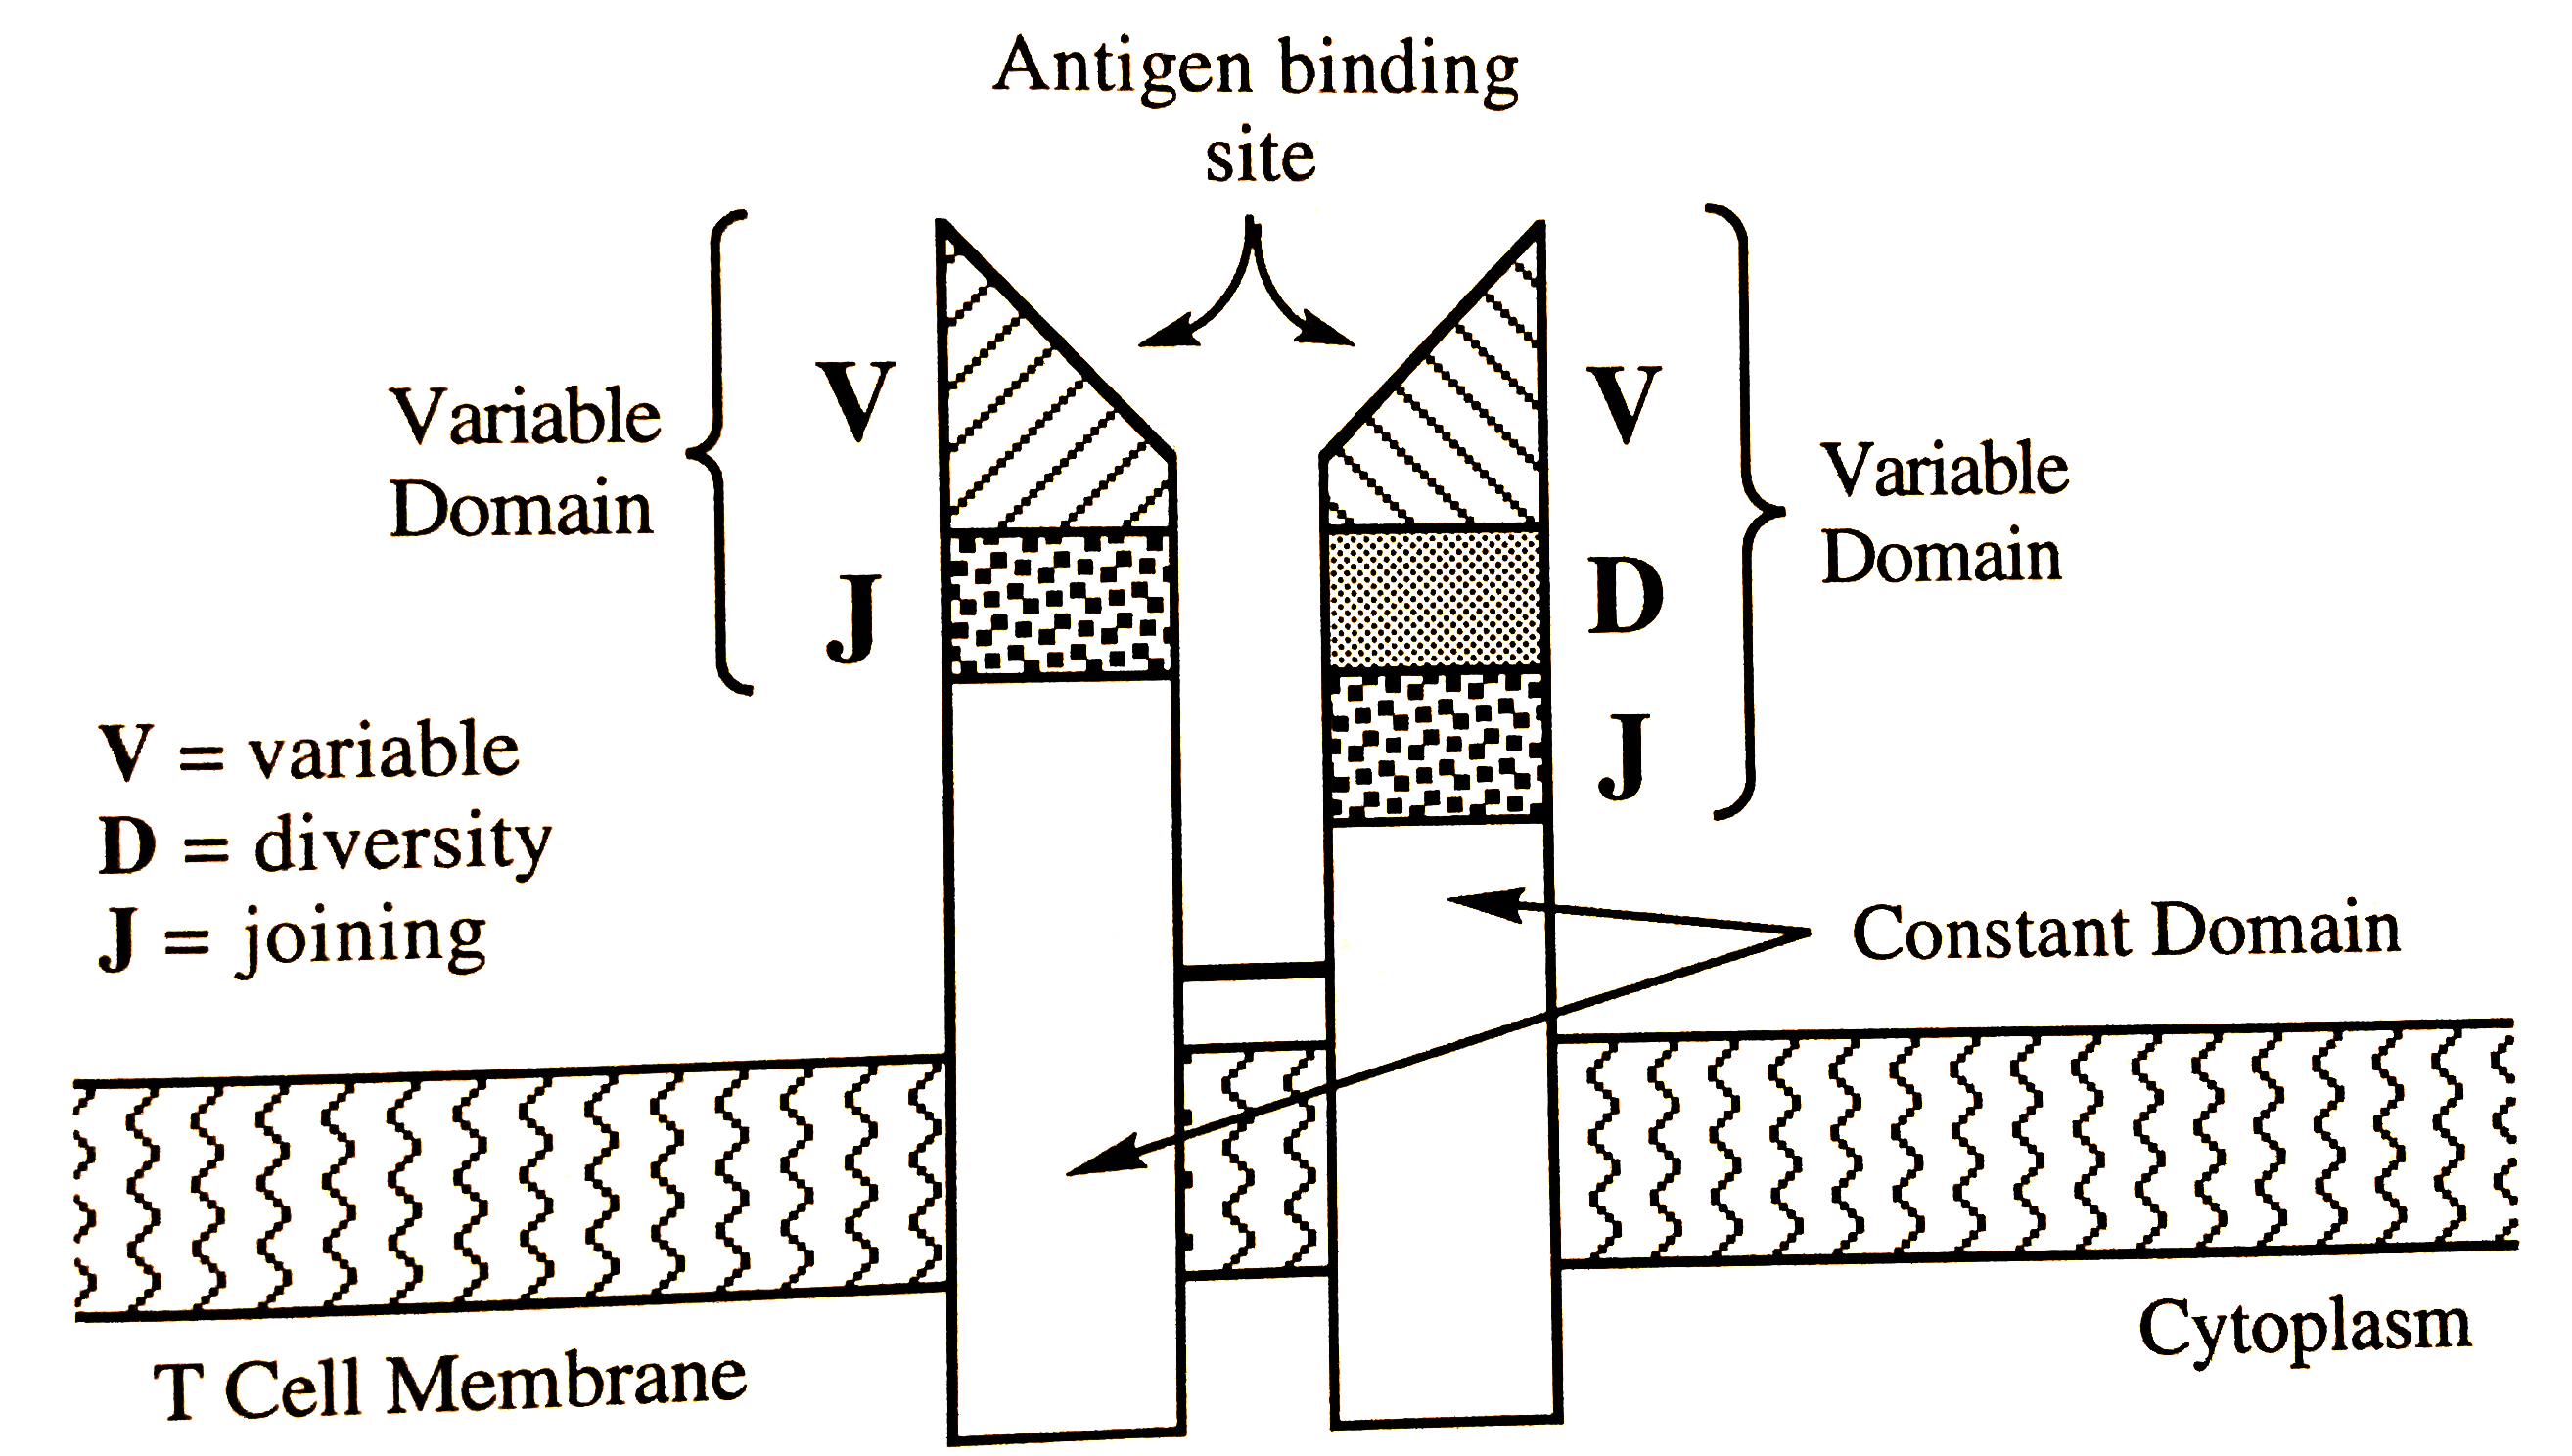
\includegraphics[width=0.55\textwidth]{t_cell_receptor.png} 
\caption{Example of T-cell Receptor Structure}
\end{figure}
\noindent If a virus infects a host cell, then that virus will begin to take over the host's metabolic machinery. As this happens some of the viral antigens are transported to the surface of the host cell where they can complex with a MHCI protein receptor, which are found on almost every one of our cells. The antigen-MHCI complex is recognized by the cytotoxic T cells, which induce lysis in the host cell. Immature helper T cells recognize macrophages which have presented an antigen on their MHCII receptors. Binding induces the macrophage to synthesize and release IL-1, which acts on the immature helper T cell and causes it to release IL-2, further stimulating the immature helper T cell to proliferate into a mature helper T cell. The mature form of the helper T cell secretes IL-2 which can activate cytotoxic T cells, B cells, and more helper T cells. 

\subsection{Immunology\textemdash Generalized Review}
Let's summarize the basic events in humoral and cellular immunity:
\begin{enumerate}
	\item A virus/bacterium enters the body by the blood and is engulfed by a macrophage.
	\item On the surface of the macrophage are MHCI receptors and MHCII receptors.
	\item A MHCII receptor presents the viral antigen to the receptor of a helper T cell, causing the macrophage to release IL-1 that stimulates the helper T cell to proliferate. 
	\item The helper T cell is stimulated to release IL-2 which enhances proliferation of helper T cells.
	\item A B cell with a MHCII protein presents viral antigen to helper T cells, and the IL-2 released from helper T cells stimulates B cells to proliferate.
	\item B cells produce plasma cells and memory B cells. Memory B cells `remember' antigen and proliferate faster during a future invasion of the same virus. Plasma cells secrete antibodies specific for the viral antigen. 
	\item The antibodies respond by direct block, complement, and cell surface coating.
	\item IL-2 from the helper T cells stimulates cytotoxic T cells which have bound to the MHCI protein-antigen complex of an infected cell to lyse the infected cell.
	\item Interferon is secreted by the infected host cell and acts on the cytotoxic T cell to help enhance the immune response.
	\item Cytotoxic T cell also make memory T cells, which will proliferate faster during a future invasion fo the same virus.
\end{enumerate}
\textbf{Fig. \ref{immune_pathway}} shows a diagram that basically summarizes the above information.
\begin{figure}[!ht]
\centering
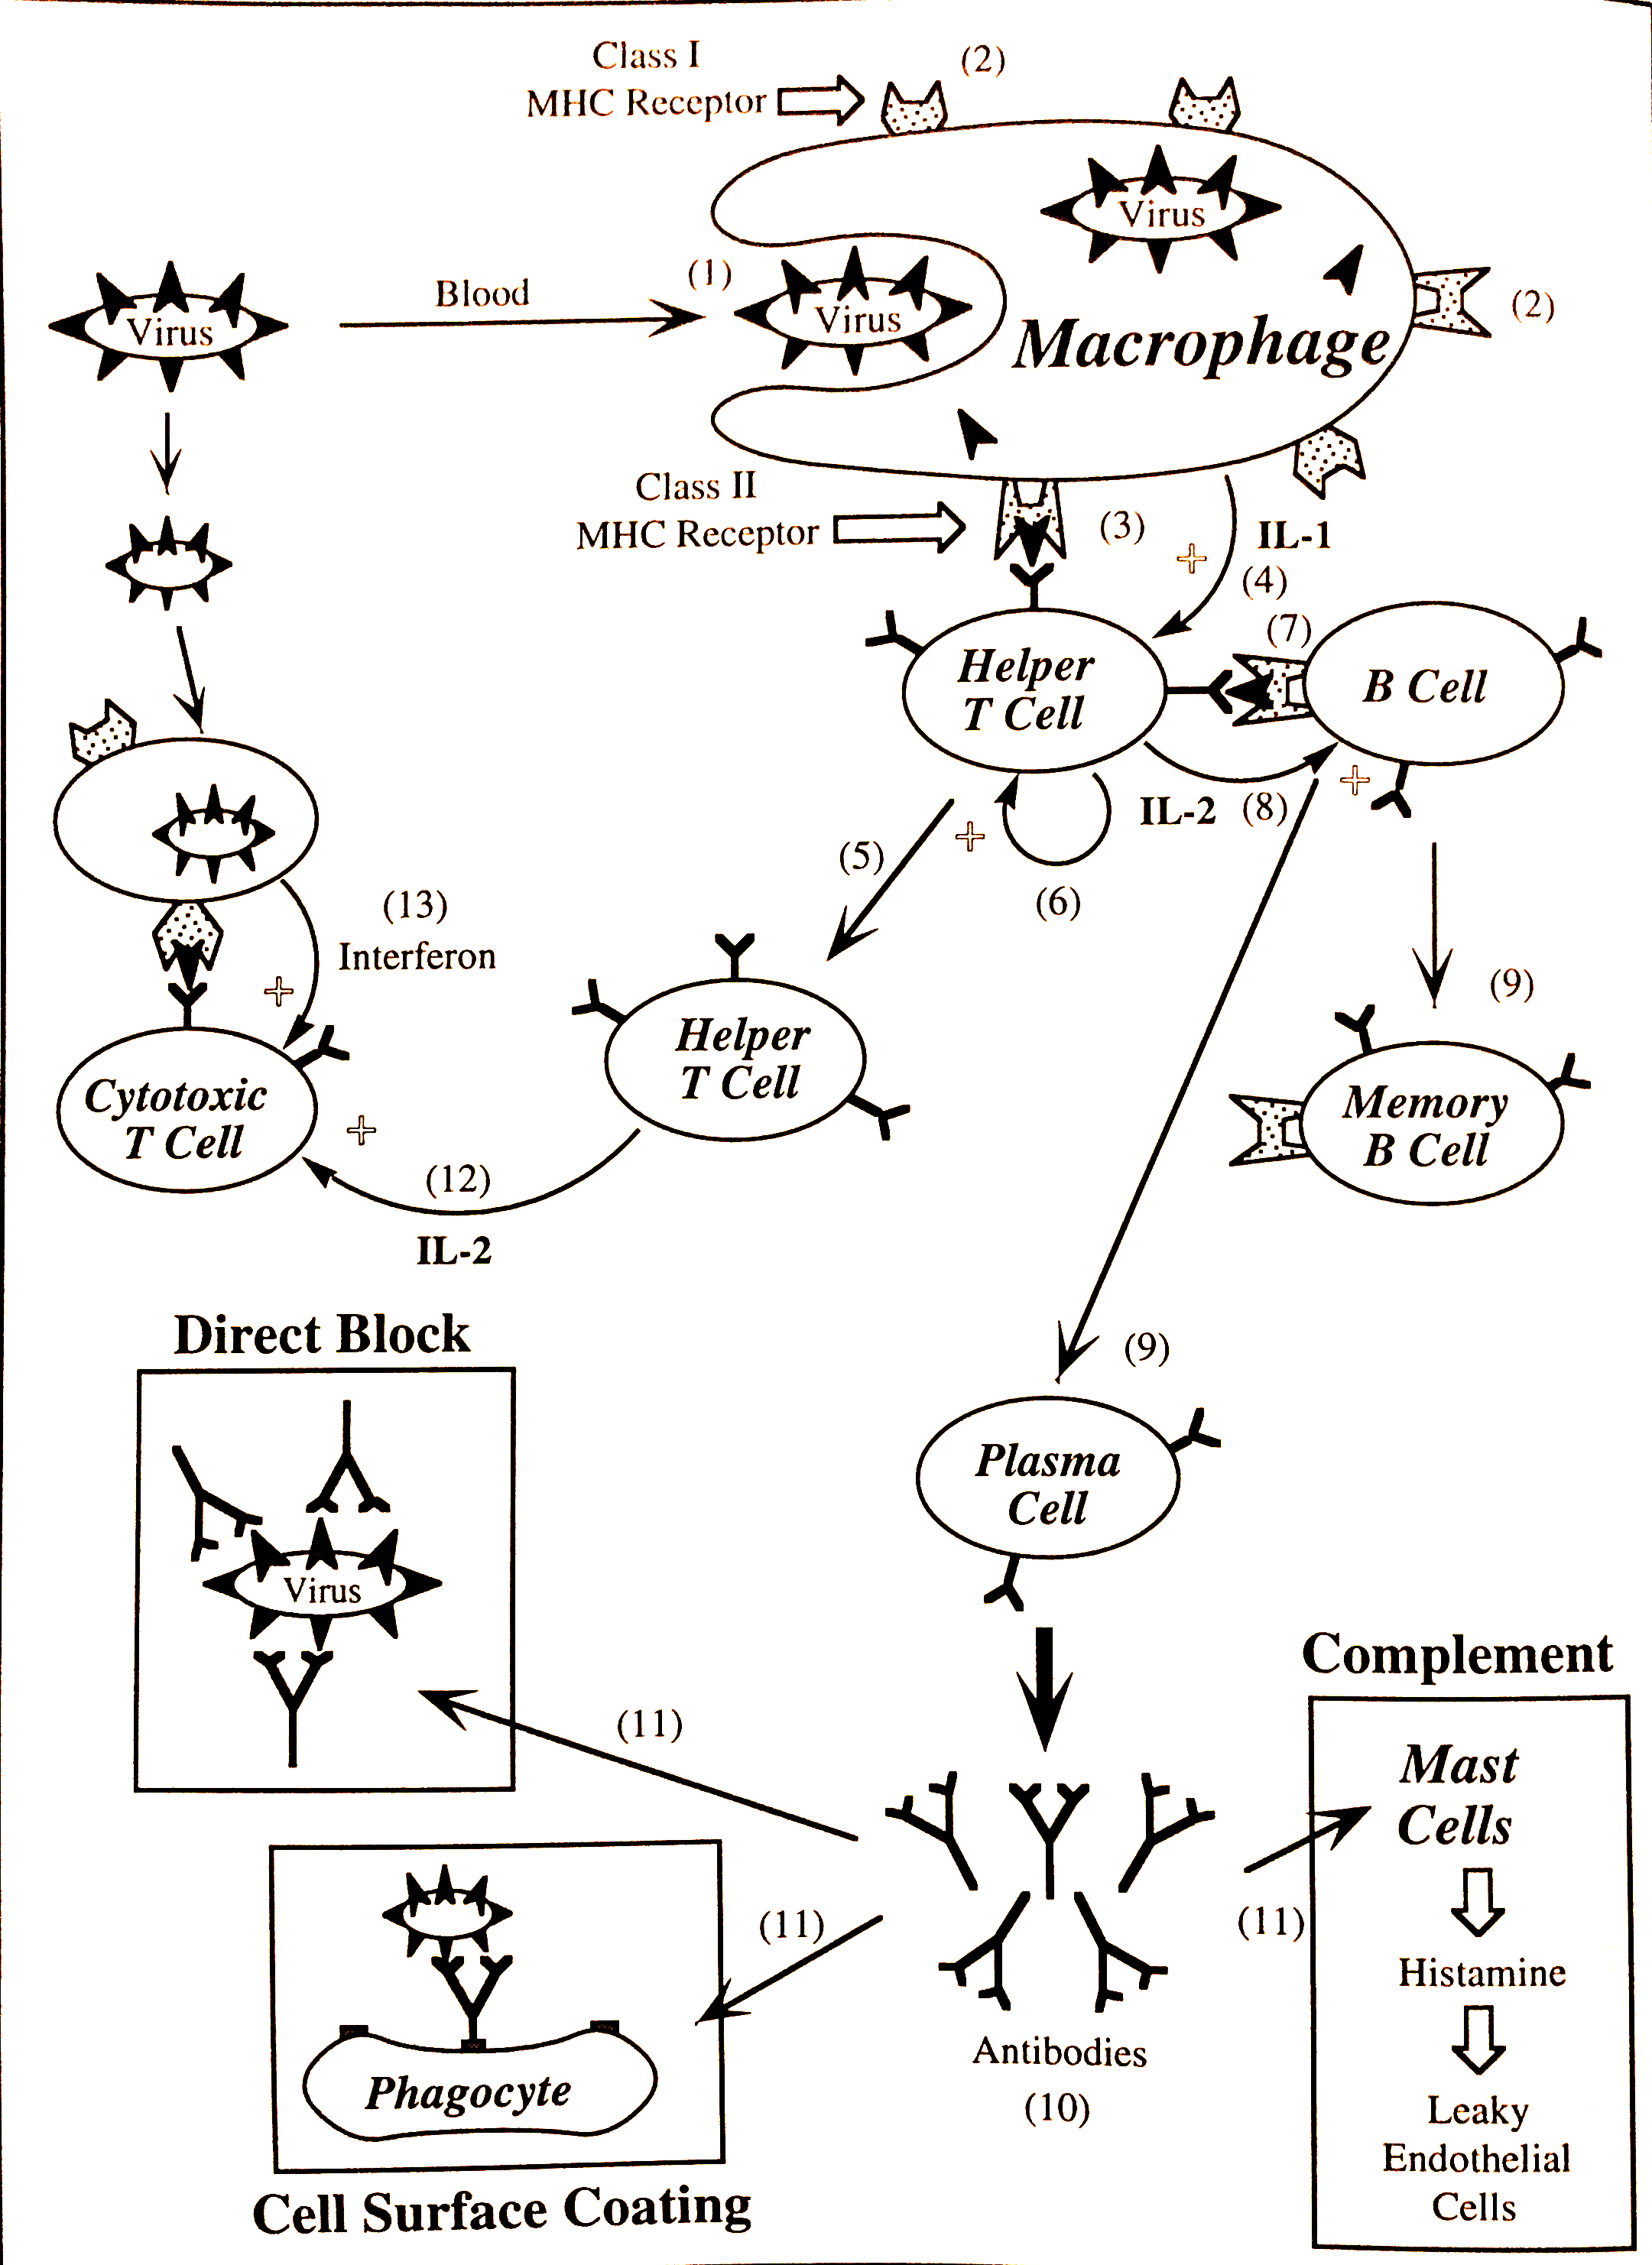
\includegraphics[width=0.7\textwidth]{immune_pathway.png} \label{immune_pathway}
\caption{Review of humoral and cellular immunity pathways.}
\end{figure}

\section{General Chemistry}
\subsection{Stoichiometry}
The MCAT does involve some math, but often it isn't too complicated. Math-related calculations required for MCAT questions involve making approximations, determining ratios, setting up calculations, and estimating the effect of errors on results. Unit conversions to memorize:
\begin{itemize}
	\item Distances: 1 m = 1.094 yd, 2.54 cm = 1 in, 1.609 km = 1 mi
	\item Masses: 1 kg = 2.205 lb, 453.6 g = 1 lb
	\item Volumes: 3.79 L = 1 gal, 1 L = 1.06 qt
	\item Temperatures: $T_F=\frac{9}{5}T_C+32, T_C=\frac{5}{9}\left(T_F-32\right)$
\end{itemize}
\indent \textbf{Molality (m)} is the concentration of a fluid solution defined as the moles of solute per kilogram of solvent. The molality of a solution does not change with temperature, so it is used to calculate the boiling-point elevation and freezing-point depression of solutions containing non-volatile impurities. \textbf{Mass percent} is the concentration of a fluid solution defined as the mass of the solute per mass of solution.\\
\indent Beer's Law is defined to be $\text{Absorbance} = \varepsilon Cl$, where $\varepsilon$ is a constant for the solute at $\lambda_{\text{max}}$ (the wavelength of greatest absorbance), $C$ is the solute concentration, and $l$ is the width of the cuvette. \\
\indent Here are some important solubility rules to remember:
\begin{enumerate}
	\item Most salts containing alkali metal cations (\ce{Li^+}, \ce{Na^+}, \ce{K^+}, \ce{Cs^+}, \ce{Rb^+}) and ammonium (\ce{NH_4^+}) are water-soluble.
	\item Most nitrate (\ce{NO_3^-}) salts are water-soluble.
	\item Most salts containing halide anions (\ce{Cl^-}, \ce{Br^-}, \ce{I^-}) are water-soluble (with heavy metal exceptions such as \ce{Ag^+} and \ce{Pb^2+}).
	\item Most salts containing sulfate anions (\ce{SO_4^{2-}}) are water-soluble (with exceptions such as \ce{Ba^2+}, \ce{Pb^2+}, \ce{Hg^2+}, and \ce{Ca^2+}). 
	\item Most hydroxide anion (\ce{OH^-}) salts are only \textit{slightly} water-soluble. \ce{KOH} and \ce{NaOH} are substantially soluble, while \ce{Ca(OH)_2}, \ce{Sr(OH)_2}, and \ce{Ba(OH)_2} are fairly soluble in water.
	\item Most carbonate anion (\ce{CO_3^{2-}}), chromate anion (\ce{CrO_4^{2-}}), phosphate anion (\ce{PO_2^{3-}}), and sulfid anion (\ce{S^2-}) salts are only slightly water-soluble.
\end{enumerate}
\indent Theres also some general test-taking tips and general advice that could prove very worthwhile:
\begin{enumerate}
	\item Keep in mind that on a multiple-choice exam, the math has been done for you, so all you need to do is approximate the answer.
	\item Intuition will prove useful on the MCAT. As you study for your MCAT, you need to learn to trust your intuition.
	\item Keep in mind that you are \textit{not} graded for showing your work on the MCAT, so don't solve every problem to the last decimal place. Analyze each question only well enough to eliminate three wrong answers. Be concise and efficient in your problem solving, not exhaustive.
\end{enumerate}

\subsection{Atomic Theory}
There are a couple of classical experiments/lab techniques that helped to develop the modern atomic theory that you should be familiar with:
\begin{enumerate}
	\item \textbf{Thomson Experiment:} This experiment helped determine the sign of charges and the charge-to-mass ratio of the electron. Basically, Thomson had a beam of electrons, and showed that he could deflect the beam by applying an electric field by an exact amount each time. The magnitude of deflection depended on the strength of the field, and reversing the plates of the external field got the same magnitude of deflection, but in the opposite direction. Thomson also figured out the charge-to-mass ratio of electrons to by $1.76\times10^8$ C/g, as the arc of deflection was constant in magnitude when the field strength was held constant but its orientation was aligned differently.
	\item \textbf{Millikan Oil Drop Experiment:} This experiment helped determine the the magnitude of charge of subatomic particles. The experimental setup involved trying to suspend a charged oil drop in an electric field. The oil drop became charged by adding an electron to it. The droplet is able to be suspended by balancing the force of gravity with and the force produced by the electric field on the charged oil droplet. Mathematically, this looks like $qE+mg=0$, so $q=-\frac{mg}{E}$. This helped determine the charge on an electron.
	\item \textbf{Rutherford Experiment:} This experiment helped determine the localization of mass/dense particles in an atom. A thin strip of gold foil lies perpendicular to an incoming stream of $\alpha$-particles. The beam strikes the gold strip surrounded by a zinc sulfide \ce{ZnS} band that luminesces if struck by $\alpha$-particles. Rutherford observed that very few $\alpha$-particles ricocheted off the gold, and most passed straight through the gold. This showed that most of an atom was empty space, and that atoms have dense nuclei with nearly all of the atomic mass centrally concentrated. 
	\item \textbf{Mass Spectrometry:} A mass spectrometer is designed to measure the charge-to-mass ratio for a charged particle. This is accomplished by sending a particle into a perpendicular magnetic field and observing the degree to which it curves. By comparing the curvature for an atomic or molecular ion to a known standard, the mass of the unknown ion and/or the mass-to-charge ratio can be determined. This is particularly helpful in determining isotopic abundance. Mathematically, the centripetal force experienced by the particle with mass $m$ is equal to the Lorentz force. Since we are given that the magnetic field $\mathbf{B}$ is always perpendicular to the particle's velocity (with magnitude $v$), this gives us $\frac{mv^2}{r}=qvB$, and solving for $r$ gives $r=\frac{mv^2}{qvB}=\frac{mv}{qB}$. The mass spectrometer embodies a simple concept\textemdash force depends on mass, so when an equal force is applied to different masses, they accelerate at different rates. The mass spectrometer takes advantage of this by accelerating charged particles in motion using a magnetic field. 
\end{enumerate}
\noindent \textbf{Heisenberg's Uncertainty Principle} states that it is not possible to simultaneously know a particle's position and velocity with infinite precision on both. Mathematically, $\Delta x\Delta p\geq \hbar/2$. The \textbf{Bohr Model} describes the transition energy of an electron between two electronic energy levels (principle quantum numbers):
\begin{equation}
\begin{split}
\Delta E=\frac{2\pi^2mZ^2e^4}{h^2}\left(\frac{1}{n_{\text{initial}}^2}-\frac{1}{n_{\text{final}}^2}\right)
\end{split}
\end{equation}
\noindent where $E$ is the energy (principle energy level), $Z$ is the nuclear charge, $n$ is the electronic energy level, $m$ is the mass of an electron, $e$ is the charge of the electron, and $h$ is Planck's constant. The important thing is that excitations (i.e. jumping up to higher energy levels) involve an input of energy, while emissions (i.e. releasing energy by going down to lower energy levels) involve the release of energy. Note also that the energies of the electronic energy levels get closer and closer as you go up. \\
\indent A \textbf{paramagnetic species} (referred to as \textit{radicals} in organic chemistry) is defined as an atom or molecule that contains at least one unpaired electron. The extra electron allows the compound to be responsive to an external magnetic field and `picking up' a magnetic moment, and so can be induced to be magnetic. A \textbf{diamagnetic species} has no unpaired electrons, and so are not susceptible to magnetic fields. Here are some important rules for electronic configurations:
\begin{enumerate}
	\item \textbf{Pauli's Exclusion Principle:} No two electrons can have the same set of quantum numbers.
	\item \textbf{Hund's Rule:} Electrons completely fill lower energy levels before starting to fill higher energy levels. In a degenerate set of orbitals, electrons singly occupy each orbital before a second electron pairs up in the same orbital.
	\item \textbf{Aufbau Principle:} Electrons are added one-by-one to the shells, starting with the lowest energy level, and then into sequentially increasing energy levels. Exceptions occur in the half-filled and filled $d$-shells, which add extra stability. For example, \ce{Cr} (chromium) has \ce{[Ar] 4s^1 3d^5} instead of \ce{[Ar] 4s^2 3d^4}, and \ce{Cu} (copper) has \ce{[Ar] 4s^1 3d^10} instead of \ce{[Ar] 4s^2 3d^9}. 
\end{enumerate}
\noindent The are four types of quantum numbers to know:
\begin{enumerate}
	\item \textbf{Principle ($n$)}: Describes the shell and energy level in which the electron resides. $n\in\mathbb{N}$.
	\item \textbf{Angular Momentum ($l$)}: Describes the orbital in which the electron resides. $l$ is a whole number less than $n$. $l=0$ is an $s$ orbital, $l=1$ is a $p$ orbital, $l=2$ is a $d$ orbital, and $l=3$ is a $f$ orbital.
	\item \textbf{Magnetic ($m_l$)}: Describes the orientation of the orbital about a plane or axis. $-l\leq m_l\leq l$.
	\item \textbf{Spin ($m_s$)}: Describes the rotation (counterclockwise or clockwise) of the electron about its axis. $m_s=\pm 1/2$.
\end{enumerate}
\noindent For $p$-orbitals ($l=1$), $m_l=-1$ corresponds to the $p_x$ orbital, $m_l=0$ corresponds to the $p_y$ orbital, and $m_l=1$ corresponds to the $p_z$ orbital. For $d$-orbitals ($l=2$), $m_l=-2$ corresponds to the $d_{xy}$ orbital, $m_l=-1$ corresponds to the $d_{xz}$ orbital, $m_l=0$ corresponds to the $d_{yz}$ orbital, $m_l=1$ corresponds to the $d_{x^2-y^2}$ orbital, and $m_l=2$ corresponds to the $d_{z^2}$ orbital. \\
\indent The \textbf{coordination number} describes the number of atoms (ligands) attached to a central atom within a molecule. Coordination numbers only count atoms attached, and \textit{not} lone pairs of electrons. For example, \ce{BH_3} has a coordination number of 3.\\
\indent When discussing excitation and relaxation, the generic case is that the energy of the photon absorbed is equal to the energy of the photon emitted. In actuality, there is more than one singular energy level for the ground state and the excited state due to the coupling of electrical energy levels and rotational energy levels associated with the atom. Transitions involve a change in electronic state as well as a change in the rotational energy of the atom. In molecules, there are vibrational energy levels to consider, in addition to the rotational and electronic energy levels. The results is that in actuality, the ground state and excited state exists as a band of energy levels, not a single level. This means that multiple possibilities exist for the energy of transition. Rather than a single line absorption or emission spectrum being formed, a range is formed. \\
\indent The atomic spectrum of hydrogen and its associated energy transitions are well studied. The \textbf{Lyman series} are the transitions that go to the $n=1$ final energy level. The \textbf{Balmer series} are the transitions that go to the $n=2$ final energy level. The \textbf{Paschen series} are the transitions that go the $n=3$ final energy level. The \textbf{Brackett series} are the transitions that go to the $n=4$ final energy level. Of these four series, only the Balmer series emits photons in the visible range. Here is an example problem: 
\begin{center}
\begin{minipage}{30em}
\textcolor{blue}{Given that the wavelength of the emitted light for the $n=3$ to $n=2$ transition in the hydrogen atom is 656 nm, which of the following is NOT true?
\begin{enumerate}[label=\Alph*]
	\item All Balmer series transitions are less than 800 nm.
	\item All Lyman series transitions are less than 400 nm.
	\item The lowest energy Paschen transition is greater than 800 nm.
	\item The highest energy Brackett transition is less than 800 nm.
\end{enumerate}}
\end{minipage}
\end{center}
\noindent Let's consider each of the answer choices one at a time:
\begin{enumerate}
	\item The Balmer series are transitions to the $n=2$ level, and the lowest energy transition is from $n=3$ to $n=2$, and is given to be 656 nm. All other transitions in the Balmer series are more energetic, so these transitions emit photons with a wavelength less than 656 nm. Therefore, choice A is valid.
	\item As a general idea, since we know that $\Delta E\propto\left(\frac{1}{n_i^2}-\frac{1}{n_f^2}\right)$, the transition of $n=2$ to $n=1$ (which is the lowest energy transition in the Lyman series by definition) as at least three times more energy change than the transition of $n=\infty$ to $n=2$. Practically, this means that all photons in the Lyman series are of higher energy and shorter wavelength than the transitions in the Balmer series. A more stringent calculation with $\Delta E=hc/\lambda$ would tell us that indeed, the transitions in the Lyman series emit photons with a wavelength less than 400 nm, meaning that choice B is valid.
	\item The Paschen series involves transitions to the $n=3$ level, and the lowest energy transition in the Paschen series is from $n=4$ to $n=3$, and it is of significantly lower energy than the $n=3$ to $n=2$ transition. This means that the lowest energy photon in the Paschen series is of lower energy and higher frequency than the transitions in the Balmer series. The Balmer series emits a photon at 656 nm, so the lowest energy transition in the paschen series emits a photon with a wavelength greater than 656 nm. Thus, choice C is a valid statment.
	\item The Brackett series involves transitions to the $n=4$ level, and from our above considerations, this should be even less energetic than the Paschen series or Balmer series. Since we showed choice C is valid, the Brackett energy transition cannot be less than 800 nm, so thus choice D is invalid and so choice \textbf{D} is the correct answer.
\end{enumerate}

\subsection{Periodic Trends}
The \textbf{effective nuclear charge} $Z_{eff}$ is the net charge exerted upon the valence electrons, which takes into account the shielding from the core electrons. As you move from left to right across a period in the periodic table, the effective nuclear charge increases. Also, as you descend a family/group in the periodic table, the valence shell increases, so the distance between the atom's valence electrons and its nucleus increases. Periodic trends depend on both $Z_{eff}$ and the valence shell. As you move up the periodic table and to the right, the following general atomic trends are observed:
\begin{enumerate}
	\item The atomic size decreases (the radius of the atom is defined as the distance from the center of the nucleus to the exterior of the valence electron cloud).
	\item The ionization energy increases (the energy required to remove the outermost electron from the atom in its gas phase).
	\item The electron affinity increases (the energetics associated with an atom gaining an electron in its gas phase).
	\item The electronegativity increases (the tendency to hold shared electrons with another atom within a bond). 
\end{enumerate}
\noindent Note that each trend shows some deviation from uniformity, some more than others. The effective nuclear charge does not uniformly increase when we scan left-to-right across a period. Half-filled stability and filled-shell stability cause some of the common deviations seen with electron affinity and ionization energy. For instance, nitrogen has a larger ionization energy than oxygen, because upon ionization, nitrogen loses its half-filled $p$-shell. On the contrary, oxygen gains half-filled stability upon being ionized.\\
\indent As a general rule, cations are smaller than neutral atoms because the loss of electrons allows the atom to compact more tightly. As a general rule, anions are larger than neutral atoms, because the gain of electrons causes the atom to expand given the enhanced repulsion associated with the additional electrons.\\
\indent Helium has a larger \textbf{atomic radius} than hydrogen. This is because the electrons in the $n=1$ level repel one another more than the electrons in any higher quantum level because they have the smallest interelectronic distance. This repulsion forces the electrons away from one another in helium, resulting in a greater area begin occupied by the orbiting electrons, and hence a greater radius for helium. \\
\indent \textbf{Ionization energy} is the energy required to remove a valence electron when the element is in the gas phase. The generic ionization reaction is represented by the equation \ce{E(g) -> E+(g) + e-}, where \ce{E} represents any element. Notable exceptions to the general ionization energy trend occur when there is half-filled stability of the energy level and where there is an $s^2$-shell. In both cases, the ionization energy is higher than expected, and also higher than the ionization energy of adjacent elements in terms of atomic number in most cases we'll be considering. \\
\indent \textbf{Electron affinity} measures the tendency of an element to gain an electron; it can be either negative or positive, meaning that gaining an electron to the valence shell can be either exothermic or endothermic. The generic reaction is represented by the equation \ce{E(g) + e- -> E-(g)}, where \ce{E} represents any element. The biggest deviations are attributed to the stability associated with a filled $s$-shell. For instance, the sudden increase in electron affinity from \ce{Be} to \ce{B}, \ce{Mg} to \ce{Al}, and \ce{Ca} to \ce{Ga} is attributed to the instability of one electron in the $p$-level. No trend for electron affinity is evident in the transition metals. \\
\indent \textbf{Electronegativity} is the ability of an atom to attract towards itself the electrons within a chemical bond. The trend in electronegativity is pretty clean, showing no exceptions at least in the first 20 elements.

\subsection{Important Periodic Families}
All alkali metals are strong reducing agents and react favorably with water in the reaction \ce{2M(s) + 2H_2O(g) -> 2MOH(aq) + H_2(g)}. The oxides they form are variable with the metal. Lithium forms \ce{Li_2O}, sodium forms a peroxide \ce{Na_2O_2}, and potassium, rubidium, and cesium form superoxides \ce{MO_2}. Alkali metals can also be oxidized into cations by halogens, nitrogen, and hydrogen. \\
\indent Alkaline earth metals are not as soluble in water as are the alkali metals in their cation form, primarily due to their \ce{2+} charge and smaller radius. They can react favorably with water (except for Be) according to the reaction \ce{M(s) + 2H_2O(g) -> M(OH)_2(aq) + H_2(g)}. The alkaline earth metals all form oxides \ce{MO} when oxidized by oxygen gas. They can also be oxidized by halogens, nitrogen, and hydrogen.\\
\indent Chalcogens are the sixth group of the periodic table that includes oxygen, sulfur, selenium, tellurium, and polonium. As neutral elements, they are oxidizing agents, but their reactivity decreases as you descend the column. Oxygen exists as a diatomic molecule \ce{O_2}, sulfur and selenium exist as octatomic molecules \ce{S_8} and \ce{Se_8}, and tellurium and polonium exist in vast molecular matrices.\\
\indent Halogens and noble gases are also important but nothing's new here. When exposed to high concentrations of fluorine gas, xenon and krypton are known to form molecular compounds with fluorine. The resulting xenon fluorides and krypton fluorides show more electron density around fluorine than the noble gas, implying that fluorine is more electronegative than either xenon or krypton. Otherwise, noble gases are pretty much unreactive. 

\subsection{Electrochemistry}
Electrochemistry addresses chemical reactions that involve electron transfer. \textbf{Galvanizing} is a protective process that involves plating a more reactive metal onto a less reactive metal, so that this more reactive species (i.e. the \textit{sacrificial metal}) is the one oxidized by air, rather than the material being protected.\\
\indent Generally speaking, organic and biological oxidizing agents are rich in oxygen and poor in hydrogen (e.g. \ce{Na_2CrO_4}, \ce{KMnO_4}, \ce{NAD+}, and \ce{FAD}), and reducing agents are poor in oxygen and rich in hydrogen (e.g. \ce{NaBH_4}, \ce{LiAlH_4}, \ce{NADH}, and \ce{FADH_2}). This is because oxidizing agents get reduced while oxidizing whatever they're reacting with, and reducing agents get oxidized while reducing whatever they're reacting with.\\
\indent The reduction of two protons (\ce{H+}) to form hydrogen gas (\ce{H_2}) is defined as the reference standard, and assigned an \textit{emf} of zero volts. Any compound that can be reduced more favorably than a proton (meaning oxidation is less favorable than a proton) has a positive reduction potential. Likewise, any compound for which reduction is less favorable than a proton (meaning oxidation is more favorable than a proton) has a negative reduction potential. Generally speaking, precious metals do not readily oxidize\textemdash thus, they have relatively high reduction potentials. On the other end of the spectrum are the alkali and alkaline earth metals, which have relatively low ionization energies, so they are easily oxidized, meaning they have negative reduction potentials. Most tables list reduction half-reaction \textit{emf} values, rather than oxidation half-reaction values. \textit{Emf} values do not need to be memorized, but in general, the greater the electron affinity, the greater the reduction potential. Likewise, a lower ionization energy corresponds to a greater oxidation potential (lower reduction potential). \\
\indent The free energy in an electrochemical cell can be described by
\begin{equation}
\begin{split}
\Delta G_{\text{reaction}}=-nF\varepsilon_{\text{cell}}
\end{split}
\end{equation}
\noindent where $F=96500$ C per mole and $n=\text{electrons per reaction}$. A positive electromotive force (cell voltage) is associated with a favorable oxidation-reduction reaction, just as a negative free energy change ($\Delta G$) is associated with a favorable oxidation-reduction reaction. \\
\indent \textbf{Electrochemical cells} convert energy produced in a chemical reaction into electrical current. Oxidation occurs at the anode, meaning that electrons flow away from the anode, and reduction occurs at the cathode (REDCAT), meaning that electrons flow towards the cathode. This means that anions migrate towards the anode and cations migrate towards the cathode through electric fields. The important thing to remember is that \textbf{electrons flow from the anode to the cathode}. There is a standard line notation for cells\textemdash when reading left to right, it goes from anode to cathode, and reactant to product within each half-reaction electrode. For example,
\begin{equation}
\begin{split}
M_{\text{oxidation}} \left(s\right) | yM \text{ } M_{\text{oxidation}}^{2+} \left(aq\right) || zM \text{ } M_{\text{reduction}}^{2+} \left(aq\right) | M_{\text{reduction}} \left(s\right)\\
\text{Reactant in anode } | \text{ Product in anode } || \text{ Reactant in cathode } | \text{ Product in cathode}
\end{split}
\end{equation}
\noindent In general, there are two types of electrochemical cells: \textbf{galvanic cells} (spontaneous cell with $\varepsilon^{\circ}>0$, $\Delta G<0$) and \textbf{electrolytic cells} (non-spontaneous cell with $\varepsilon^{\circ}<0$, $\Delta G>0$, and an applied voltage present to power the cell). Galvanic cells release energy in the form of electrical flow, while electrolytic cells are used for the storage of electrical potential, as is seen when recharging a battery. \\
\indent The \textbf{Nernst equation} is often used to quantify the effect of concentration on the voltage of an electrochemical cell. Mathematically, it is
\begin{equation}
\begin{split}
\varepsilon_{\text{cell}}=\varepsilon^{\circ}-\frac{RT}{nF}\ln Q_{rx}
\end{split}
\end{equation}
\noindent By substituting $R=8.314 \text{J}/\text{mol}\cdot\text{K}$, $T=298$ K, and $F=96500$ C/mol, we get the working equation 
\begin{equation}
\begin{split}
\varepsilon_{\text{cell}}=\varepsilon^{\circ}-\frac{0.059}{n}\log_{10} Q_{rx}
\end{split}
\end{equation}
\noindent where we're being pretty lenient with the units. Note that our working equation has $\log_{10}$ instead of $\ln$ natural logarithm. Here is an example problem using the Nernst equation:
\begin{center}
\begin{minipage}{30em}
\textcolor{blue}{What is the voltage of an electrochemical cell with an anode of zinc metal in 0.01 M \ce{Zn(NO_3)_2} (aq) and a cathode of silver metal in 1.00 M \ce{AgNO_3} (aq)?
\begin{enumerate}[label=\Alph*]
	\item 2.42 V
	\item 2.30 V
	\item 1.62 V
	\item 1.50 V
\end{enumerate}}
\end{minipage}
\end{center}
\noindent First, we must identify the half-reaction:
\begin{equation}
\begin{split}
\text{Oxidation:}\quad \ce{Zn(s)}\rightarrow\ce{Zn^2+}+2\ce{e-}, \quad\quad \ce{Ag+}+\ce{e-}\rightarrow\ce{Ag(s)}
\end{split}
\end{equation}
The standard cell potential for the reaction is found using values from online or a provided table (not the important part here), and we get $\varepsilon^{\circ}=0.80 \text{ V}-\left(-0.76\text{ V}\right)=1.56 \text{ V}$. The actual cell voltage is slightly higher than $1.56$, because there is a higher cation concentration in the cathode than in the anode. The exact value is found using the Nernst equation:
\begin{equation}
\begin{split}
\varepsilon_{\text{cell}}=\varepsilon^{\circ}-\frac{0.059}{n}\log\frac{[\ce{Zn^2+}_{\text{anode}}]}{[\ce{Ag+}_{\text{cathode}}]^2}=1.56\text{ V }-\frac{0.059}{2}\log\frac{0.01}{1^2}=\left(1.56 - 0.03(\log 0.01)\right)\text{ V}=\left(1.56+0.06\right)\text{ V}=1.62 \text{V}
\end{split}
\end{equation}
\noindent giving us the answer choice \textbf{C} as the correct answer, as desired. 

\subsection{Gases and Gas Laws}
The \textbf{collision force} is defined as the force exerted by a gas particle during a collision between it and the container wall. It is based on impulse, so both greater momentum and a shorter time of contact increase the force of impact. The collision force can be increased by increasing the temperature, because greater temperature imparts greater velocity, and thus greater momentum, to each molecule. The \textbf{mean free path} is defined as the average distance a particle can travel before colliding with another particle. There are three key assumptions associated with the \textbf{Kinetic Molecular Theory of Gases}:
\begin{enumerate}
	\item Particles are so small compared to the distances between particles that their volumes are negligible.
	\item Particles move in straight lines, and there are no intermolecular forces. The collisions are said to be elastic with no energy dissipation.
	\item Particles are in constant random translational motion.
\end{enumerate}
\noindent An ideal gas is a theoretical gas that obeys all of these conditions. In a gas system, not all particles have the same kinetic energy\textemdash there is a random distribution of energies defined by the temperature-dependent \textit{Boltzmann distribution}. Of course, no gas is truly ideal, and we have the \textbf{van der Waals equation} to describe real gases:
\begin{equation}
\begin{split}
\left(P_{\text{observed}}+a\frac{n^2}{V^2}\right)\left(V_{\text{container}}-nb\right)=nRT
\end{split}
\end{equation}
\noindent where $a$ is the \textbf{attraction coefficient} ($a>0$ is particles attracting, $a<0$ is particles repelling), $b$ is the `\textbf{bigness coefficient}' ($b>0$ for all particles). Here are two sample problems regarding the van der Waals equation:
\begin{center}
\begin{minipage}{30em}
\textcolor{blue}{Which of the following types of gases has a negative $a$ term?
\begin{enumerate}[label=\Alph*]
	\item Polar
	\item Nonpolar
	\item Hydrophobic
	\item Ionized
\end{enumerate}}
\end{minipage}
\end{center}
\noindent An ionized gas has particles that all have the same charge, and like charges repel, so choice \textbf{D} is the best answer.
\begin{center}
\begin{minipage}{30em}
\textcolor{blue}{Which of the following types of gases has the greatest $b$ term?
\begin{enumerate}[label=\Alph*]
	\item Methane
	\item Ethane
	\item Ethene
	\item Ethyne
\end{enumerate}}
\end{minipage}
\end{center}
\noindent Ethane has the greatest mass of the given molecules, and so it has the greatest $b$ term. Thus, the answer is \textbf{B}. \\
\indent Here's another practice problem, this time regarding how to measure pressure using a manometer and using the equation $\Delta P=\rho g \Delta h$:
\begin{center}
\begin{minipage}{30em}
\textcolor{blue}{What is the pressure in atmospheres of a column of gas in a closed tube above mercury if the height difference at sea level between a connected column of mercury open to the atmosphere and the closed column above mercury is 317 mm?
\begin{enumerate}[label=\Alph*]
	\item 317/760 atm
	\item 443/760 atm
	\item 760/443 atm
	\item 317/443 atm
\end{enumerate}}
\end{minipage}
\end{center}
\noindent The height difference of 317 mm means that the pressure difference is 317 torr (mm Hg, by definition). The atmospheric pressure at sea level is 760 torr, so the gas pressure in the column is $760-317=443$ torr. The conversion from torr to atm involves dividing by a factor of 760 torr per atm, making choice \textbf{B} the best answer. As the question is worded, the pressure difference is provided, but the relative pressure are not mentioned. The pressure could also be $760+317=1077$ torr, but this value is not listed as an answer choice.\\
\indent The \textbf{root mean square speed} of a gas is 
\begin{equation}
\begin{split}
\mu_{\text{rms}}=\sqrt{\frac{3RT}{m}}
\end{split}
\end{equation}
\noindent where $R$ is the ideal gas constant, $T$ is the temperature, and $m$ is the mass of one mole of the gas. This is derived by solving the equation $\frac{1}{2}mv^2=\frac{3}{2}RT$ for $v$, as the left hand side is the kinetic energy from classical mechanics and the right hand side is the energy of the system obtained through the equipartition theorem. Here is an example problem:
\begin{center}
\begin{minipage}{30em}
\textcolor{blue}{What is the root mean square speed of neon atoms at $27^{\circ}$C?
\begin{enumerate}[label=\Alph*]
	\item 19.3 m/s
	\item 211 m/s
	\item 612 m/s
	\item 1018 m/s
\end{enumerate}}
\end{minipage}
\end{center}
\noindent From the periodic table, the mass of one mole of neon is $m=0.20$ kg, and the temperature converted to Kelvin is $T=300$ K. Thus,
\begin{equation}
\begin{split}
\mu_{\text{rms}}=\sqrt{\frac{3RT}{m}}=\sqrt{\frac{3\left(8.314\right)\left(300\right)}{0.020}}=\sqrt{\frac{\left(8.314\right)\left(9\times10^2\right)}{2\times10^{-2}}}\approx \sqrt{\frac{8\times9}{2}\times 10^4}=\sqrt{36\times 10^4}=6\times10^2=600 \text{m/s}
\end{split}
\end{equation}
\noindent where we ignore the units for convenience. Thus, the best answer is choice \textbf{C}. Using this formula for the root mean square speed, we can determine the relative speeds of two gases, giving us \textbf{Graham's law} for gas flow:
\begin{equation}
\begin{split}
\frac{v_2}{v_1}=\sqrt{\frac{m_1}{m_2}}
\end{split}
\end{equation}
\noindent which holds for a given temperature. This equation is basically saying that the speed of the particle is inversely proportional to the square root of its mass, so the lighter the gas, the faster it travels at a given temperature. There is also the relationship
\begin{equation}
\begin{split}
\frac{v_2}{v_1}=\sqrt{\frac{T_2}{T_1}}
\end{split}
\end{equation}
\noindent which holds for a given mass of particles. This is basically saying that the speed of the particle is directly proportional to the square root of the temperature, so the greater the temperature, the faster a gas travels.

\subsection{Phases and Phase Changes}
\textbf{Isochoric} conditions are where the \textit{volume} of the system does not change, and \textbf{adiabatic} conditions are where \textit{heat} nether enters nor exits the system, meaning that the system is perfectly insulated. The \textbf{critical point} is the highest temperature and pressure at which a liquid may be observed. Beyond the critical point, it is impossible to distinguish between a gas and a liquid, so it is referred to as a \textit{supercritical fluid}. The \textbf{triple point} is where all three phases of matter can exist for a given compound. It is also the highest temperature and pressure at which sublimation (and deposition) can occur. Two key facts of water are that its liquid form is denser than its solid form, and it is densest at $4^{\circ}$C. \\
\indent The enthalpy of vaporization is greater in magnitude than the enthalpy of fursion because more energy is necessary to \textit{break} the intermolecular forces (i.e. for liquid $\rightarrow$ gas) than is necessary to weaken the intermolecular forces (i.e. for solid $\rightarrow$ liquid).\\
\indent The formal definition of \textbf{vapor pressure} above a liquid is the force per unit area above the surface of a liquid exerted by molecules formed upon evaporation of the liquid. Vapor pressure can be measured in either an open or closed system. In a closed system, a partial pressure of vapor exists, because the rate of vaporization equals the rate of condensation. This is most typically how vapor pressure is determined. In an open system, since no equilibrium is reached, vapor pressure is a measure of the pressure just above the surface of the liquid. Vapor pressure is \textit{independent} of the shape and volume of a container. Vapor pressure increases as temperature increases, and decreases as the heat of vaporization $\Delta H_{\text{vaporization}}$ increases. The \textbf{Clausius-Clapeyron} equation can be used to explain the relationship between vapor pressure and temperature:
\begin{equation}
\begin{split}
\ln \frac{p_1}{p_2}=\frac{\Delta H_{\text{vaporization}}}{R}\left(\frac{1}{T_2}-\frac{1}{T_1}\right)
\end{split}
\end{equation}
\noindent The conclusion from this is that as the temperature of a liquid increases, the pressure of its vapor increases in an exponential manner. This equation assumes that the heat of vaporization $\Delta H_{\text{vaporization}}$ is constant over the temperature range of interest. Detailed calculations involving the Clausius-Clapeyron equation are unlikely, but it should still be understood conceptually and graphically.\\
\begin{equation}
\begin{split}
\text{As } \Delta H_{\text{vaporization}}\uparrow; \text{ Volatility } \downarrow; \text{ Boiling Point } \uparrow; \text{ Vapor Pressure} \downarrow
\end{split}
\end{equation}
\noindent The \textbf{boiling point} is defined as the temperature at which the vapor pressure is equal to the atmospheric pressure. According to \textbf{Raoult's Law}, the vapor pressure above a solution of two or more \textit{miscible} liquids depends on the mole fraction of each compound in solution. Mathematically,
\begin{equation}
\begin{split}
P_{\text{vapor}}=\xi_iP_{\text{vapor (pure)}}
\end{split}
\end{equation}
\noindent where the $\xi_i$ in Raoult's equation is the mole fraction of the component \textit{in solution}, not in the vapor state. With real compounds, because of intermolecular forces within liquids, there are other factors that come into play. The molecules interact in both the liquid and gas phases, so the vapor pressure relationship is not \textit{exactly} linear as Raoult's equation approximates it to be. Intermolecular forces are greater in the solution than the gas phase. If there is an overall increase in attractive forces in solution whent he components are mixed, then vaporization, and thus vapor pressure, decreases, resulting in a negative deviation from linearity. Likewise, if there is an overall decrease in attractive forces in solution when the components are mixed, then vaporization, and thus vapor pressure, increases, resulting in a positive deviation from linearity. \textbf{Distillation} is removing a liquid from a solution by utilizing their differing vapor pressures/boiling points. 

\subsection{Colligative Properties}
Colligative properties are properties of a solution that are affected by the concentration of a soluble impurity. Colligative properties include boiling point elevation, freezing point depression, and osmotic pressure. The electrical conductivity of a solution, although it is not formally a colligative property, shows a dependence on ion concentration. The increase in boiling point $\Delta T_b$ when solute is added to a solution is given by
\begin{equation}
\begin{split}
\Delta T_b=k_b\cdot i\cdot m
\end{split}
\end{equation}
\noindent where $i$ is the number of ions that form upon dissolving, $m$ is the \textit{molality} of the solution, and $k_b$ is a constant for the solvent. Similarly, we also have the equation for freezing point depression which basically looks that same as that for boiling point elevation:
\begin{equation}
\begin{split}
\Delta T_f=k_f\cdot i\cdot m
\end{split}
\end{equation}
\noindent Note that $\Delta T_f<0$ and $\Delta T_b>0$ (that's why its called freezing point \textit{depression} and boiling point \textit{elevation}).\\
\indent Water has a natural tendency to flow from solutions of higher water concentration (i.e. lower solute concentration) to solutions of lower water concentration (i.e. higher solute concentration) to reach equal concentrations. Pressure differences cause fluids like water to flow, and the driving force causing water to flow is known as \textbf{osmotic pressure}. Osmotic pressure $\pi$ is the pressure exerted by a solution through osmosis across a semipermeable membrane, and is given by
\begin{equation}
\begin{split}
\pi=MiRT
\end{split}
\end{equation}
\noindent where $M$ is the \textit{molarity}, $i$ is the number of ions upon dissociation, $R$ is the ideal gas constant, and $T$ is the temperature. The \textbf{condosity} of a solution is defined as the molar concentration of an aqueous sodium chloride solution that has the same specific conductance as the aqueous salt solution. 

\subsection{Solubility}
A \textbf{supersaturated} solution is where the amount of solute that is dissolved into solution is beyond the maximum amount at that given temperature. The solution is actually a suspension that when disturbed can form a precipitate rapidly. This state can be achieved by first heating a solvent, then adding solute to the solution until the solution is saturated at that temperature. Slowly cooling this solution causes the amount of solute in it to exceed that should dissolve at the reduced temperature. \textbf{Gram solubility} is the quantitative measurement of the maximum number of grams of solute that can dissolve into enough solvent to make one hundred mL of solution under ambient conditions. Here are the solubility rules you should know:
\begin{enumerate}
	\item Most salts composed of +1 cation (excluding transition metals) and -1 anion are soluble in water at room temperature. Nitrate \ce{NO_3-} salts are water-soluble.
	\item Most salts containing sulfate \ce{SO_4^{2}-} anions \textit{with +1 cations} (excluding transition metals) are water-soluble.
	\item Most salts with -2 or -3 anions are insoluble in water (excluding sulfate salts).
	\item Most oxide \ce{O^{2}-} and hydroxide \ce{OH-} anion salts are only slightly water soluble. \ce{KOH} and \ce{NaOH} are notable exceptions that are substantially water soluble. 
\end{enumerate}
\noindent An \textbf{ion-exchange} column exchanges one ion in solution for another (which is initially bound to the column), by precipitating out the ion that forms the less soluble salt and releasing a more soluble into solution to replace it. A water softener is a good example of an ion-exchange column\textemdash hard water (rich in \ce{Ca^{2}+(aq)}) travels down the column where the anion in the ion-exchange resin binds calcium cations to form an insoluble salt while releasing sodium cations \ce{Na+(aq)} into solution. Aqueous sodium cation is referred to as soft water. As calcium precipitates through the column, it is filtered from the water, preventing it from forming precipitates in the plumbing lines of appliances. The reaction that we're interested in is \ce{2Na+(aq) + CaCl_2(s) <-> Ca^{2}+(aq) + 2NaCl (s)}; this reaction highly favors the reactants side. There's also another thing called \textbf{selective precipitation and ion exchange}, where we add an ion to solution with the intention of precipitating an existing ion out of the solution. This is basically the same thing as the ion-exchange column, and can be achieved when the salt being precipitated is less soluble than any other salt combination in solution. For example, consider the reaction \ce{2AgCl(s) + Hg^{2}+(aq) <-> 2Ag+(aq) + HgCl_2(s)}. Because mercury chloride is less soluble than silver chloride, the addition of silver chloride to the mercury solution precipitates mercury out of water.\\
\indent When reactions are added together, the equilibrium constant $K$ fot eh overall reaction is the product of the equilibrium constants of the component reactions. Here is an example problem for solubility:
\begin{center}
\begin{minipage}{30em}
\textcolor{blue}{Silver chloride \ce{AgCl} is MOST soluble in which of the following solutions at $25^{\circ}$C?
\begin{enumerate}[label=\Alph*]
	\item 0.10 M \ce{HgNO_3(aq)}
	\item Pure water
	\item \ce{AgNO_3(aq)}
	\item \ce{NaCl}
\end{enumerate}}
\end{minipage}
\end{center}
As discussed above, silver chloride is most soluble in a solution where \ce{Hg+(aq)} is present, as the mercury ion in solution can bind the chloride anion to form a precipitate. As the amount of \ce{Cl-} in solution decreases as a result, more \ce{AgCl} dissolves into solution to replace it. Thus, the best answer is choice \textbf{A}. Both choices C and D are eliminated because of the common ion effect. 

\subsection{Acids and Bases}
The \textbf{haloacids} are the series of \ce{HX} acids, where \ce{X} represents a halogen. As the size of the halogen increases, the haloacid becomes more acidic due to the increased stability of the conjugate base halide as it increases in size. Dissociation increases, bond strength decreases, and bond length increases as \ce{X} gets bigger. \\
\indent Within a period of the periodic table, it is electronegativity that dictates the strength of an acid, \textit{not} atomic radius. A prime example of this idea is the relationship between ammonia \ce{H-NH_2}, water \ce{H-OH}, and hydrofluoric acid \ce{H-F}. The strongest acid of the three is \ce{HF}, because fluorine is more electronegative than oxygen or nitrogen. The atomic size doesn't change that noticeably between the three elements\textemdash the periodic trend that changes the most from \ce{N} to \ce{F} is the electronegativity.\\
\indent To determine how much acid (or base) is necessary to neutralize a solution of base (or acid), use $M_1V_1=M_2V_2$. Make sure to take into account if the acid is polyprotic/the base has multiple hydroxide groups or something like that. Here is an example problem:
\begin{center}
\begin{minipage}{30em}
\textcolor{blue}{Citric acid (\ce{C_6H_8O_7}) has three dissociable protons with \ce{pK_a} values of 3.14, 4.79, and 5.20. Which of the following solutions would have the lowest pH value?
\begin{enumerate}[label=\Alph*]
	\item 50 mL 0.10 M citric acid (aq) + 75 mL 0.20 M \ce{NaOH(aq)}
	\item 25 mL 0.10 M citric acid (aq) + 50 mL 0.10 M \ce{NaOH(aq)}
	\item 25 mL 0.20 M citric acid (aq) + 75 mL 0.20 M \ce{NaOH(aq)}
	\item 50 mL 0.20 M citric acid (aq) + 50 mL 0.10 M \ce{NaOH(aq)}
\end{enumerate}}
\end{minipage}
\end{center}
\noindent The lowest pH belongs to the solution that is most acidic, and the most acidic solution is the one where the fewest equivalents of base relative to citric acid have been added. In choice D, the \ce{NaOH(aq)} solution is of equal volume and half the concentration of the citric acid solution, so there is only one-half of an equivalent of \ce{NaOH(aq)}. Comparing this with the other answer choices, this is the lowest number of equivalents of the base compared to the other answer choices, so thus, choice \textbf{D} is the best answer.\\
\indent In a solution, the distribution within a conjugate pair is dictated by the pH of the solution. The conjugate pair favors the conjugate acid form in the presence of hydronium, and favors the conjugate base form in the presence of hydroxide. In general, if pH>pK\textsubscript{a}, the solution is basic relative to the compound, so it exists predominantly in its deprotonated form (\ce{[A-]}>\ce{[HA]}). If pH<pK\textsubscript{a}, the solution is acidic relative to the compound, so it exists predominantly in its protonated form (\ce{[A-]}<\ce{[HA]}). 
\begin{center}
\begin{minipage}{30em}
\textcolor{blue}{What is the pK\textsubscript{a} for ammonia \ce{NH_3}, given that the pK\textsubscript{b} for ammonia is 4.7?
\begin{enumerate}[label=\Alph*]
	\item 4.7
	\item 7.0
	\item 9.3
	\item 33
\end{enumerate}}
\end{minipage}
\end{center}
\noindent \textbf{It is not 9.3!} The compound with a pK\textsubscript{a} of 9.3 is ammonium (\ce{NH_{4}+}), the conjugate acid of ammonia. Ammonia is a weaker acid than ammonium, so it has a pK\textsubscript{a} greater than 9.3. The best answer is 33, choice \textbf{D}, indicating that ammonia is such a weak acid that when added to water, there is no detectable dissociation. The mistake of choosing 9.3 is easy to make, one that most students make routinely. However, the equation pK\textsubscript{a, (HA)}+pK\textsubscript{b (A\textsuperscript{-})}=14 is for conjugate pairs, not for the same compound. The pH of a solution composed of both components in a weak conjugate pair can be determined using the \textbf{Henderson-Hasselbalch} equation:
\begin{equation}
\begin{split}
\ce{pH}=\ce{pK_a}+\log\frac{\ce{[HA]}}{\ce{[A-]}}
\end{split}
\end{equation}
\noindent The equation shows that as the conjugate base concentration \ce{[HA]} increases, the pH of the buffer increases.

\subsection{Titration Curves}
A \textbf{buffer} is a solution whos pH remains relatively constant after the addition of either strong acid or strong base. The pH may vary slightly, but for all intents and purposes, it does not change significantly. The pH of a buffered solution is determined using the Henderson-Hasselbalch equation, as discussed in the previous section. Buffers are made of a roughly equal mole mixture of a weak acid and its weak conjugate base in an aqueous solution. The pH range of a buffer is pH$\in[\text{pK\textsubscript{a}}-1, \text{pK\textsubscript{a}}+1]$. Buffers can be made by mixing any of the following things together:
\begin{enumerate}
	\item Weak acid + the salt of the conjugate base in roughly equal mole proportions (e.g. \ce{HCO_2H} with \ce{HCO_2Na}). 
	\item Weak base + the salt of the conjugate acid in roughly equal mole proportions (e.g. \ce{NH_3} with \ce{NH_4Cl}).
	\item Weak acid + roughly half of an equivalent of strong base (e.g. \ce{HOAc} with a half-equivalent of \ce{KOH}).
	\item Weak base + roughly half of an equivalent of strong acid (e.g. \ce{H_3CNH_2} with a half-equivalent of \ce{HCl}).
\end{enumerate}
\noindent Physiological pH is considered to be 7.4 and is usually highly buffered in most regions of the body. In a \textit{titration}, the \textbf{equivalence point} is reached when the moles of acid are equal to the moles of base. Here are a couple of good practice problems for titrations:\\
\begin{center}
\begin{minipage}{30em}
\textcolor{blue}{What is the pH after 30 mL of 1.00 M \ce{NaOH(aq)} have been added to 100 mL 0.50 M \ce{HOAc(aq)}? \ce{HOAc} has a pK\textsubscript{a}=4.74.
\begin{enumerate}[label=\Alph*]
	\item 3.51
	\item 4.56
	\item 4.92
	\item 5.97
\end{enumerate}}
\end{minipage}
\end{center}
\noindent Because the strong base is twice as concentrated as the weak acid, only half the volume of strong base (relative to the weak acid) is required to reach the equivalence point. This means that 50 mL of 1.00 M \ce{NaOH} fully neutralizes the 100 mL of 0.50 M \ce{HOAc}. The halfway point of the titration is therefore reached when exactly 25 mL of 1.00 M \ce{NaOH} have been added. At the halfway point, the pH of the solution equals the pK\textsubscript{a} of the weak acid. The additional strong base beyond the 25 mL makes the pH of the solution slightly greater than the pK\textsubscript{a} of the acid, 4.74. Thus, the best choice is answer \textbf{C}. Here is another problem:
\begin{center}
\begin{minipage}{30em}
\textcolor{blue}{What is the pH of a solution made by mixing 10.0 mL 0.10 M \ce{HCO_2H(aq)} with 4.0 mL 0.10 M \ce{KOH(aq)}? The pK\textsubscript{a} of \ce{HCO_2H} is 3.64.
\begin{enumerate}[label=\Alph*]
	\item 1.34
	\item 3.46
	\item 3.82
	\item 9.36
\end{enumerate}}
\end{minipage}
\end{center}
\noindent The weak acid and titrant strong base are of equal concentration, so 10 mL \ce{KOH} is one equivalent (the amount needed to reach the equivalence point). If 5.0 mL are added, then the acid is half-titrated, so pH=pK\textsubscript{a}. However, less than 5.0 mL have been added, so the pH is a little less than pK\textsubscript{a}. The pK\textsubscript{a} is given to be 3.64, so the best answer is choice \textbf{B}. Choice A is too much less than the pK\textsubscript{a}. \\
\indent Polyprotic acids yield multiple equivalents of hydronium ion per molecule, and so therefore have multiple equivalence points, one of each dissociable proton. Each equivalence point is the arithmetic mean of the two adjacent pK\textsubscript{a} values. This is clearly shown in \textbf{Fig. \ref{polyprotic}}. \\
\begin{figure}[!ht]
\centering
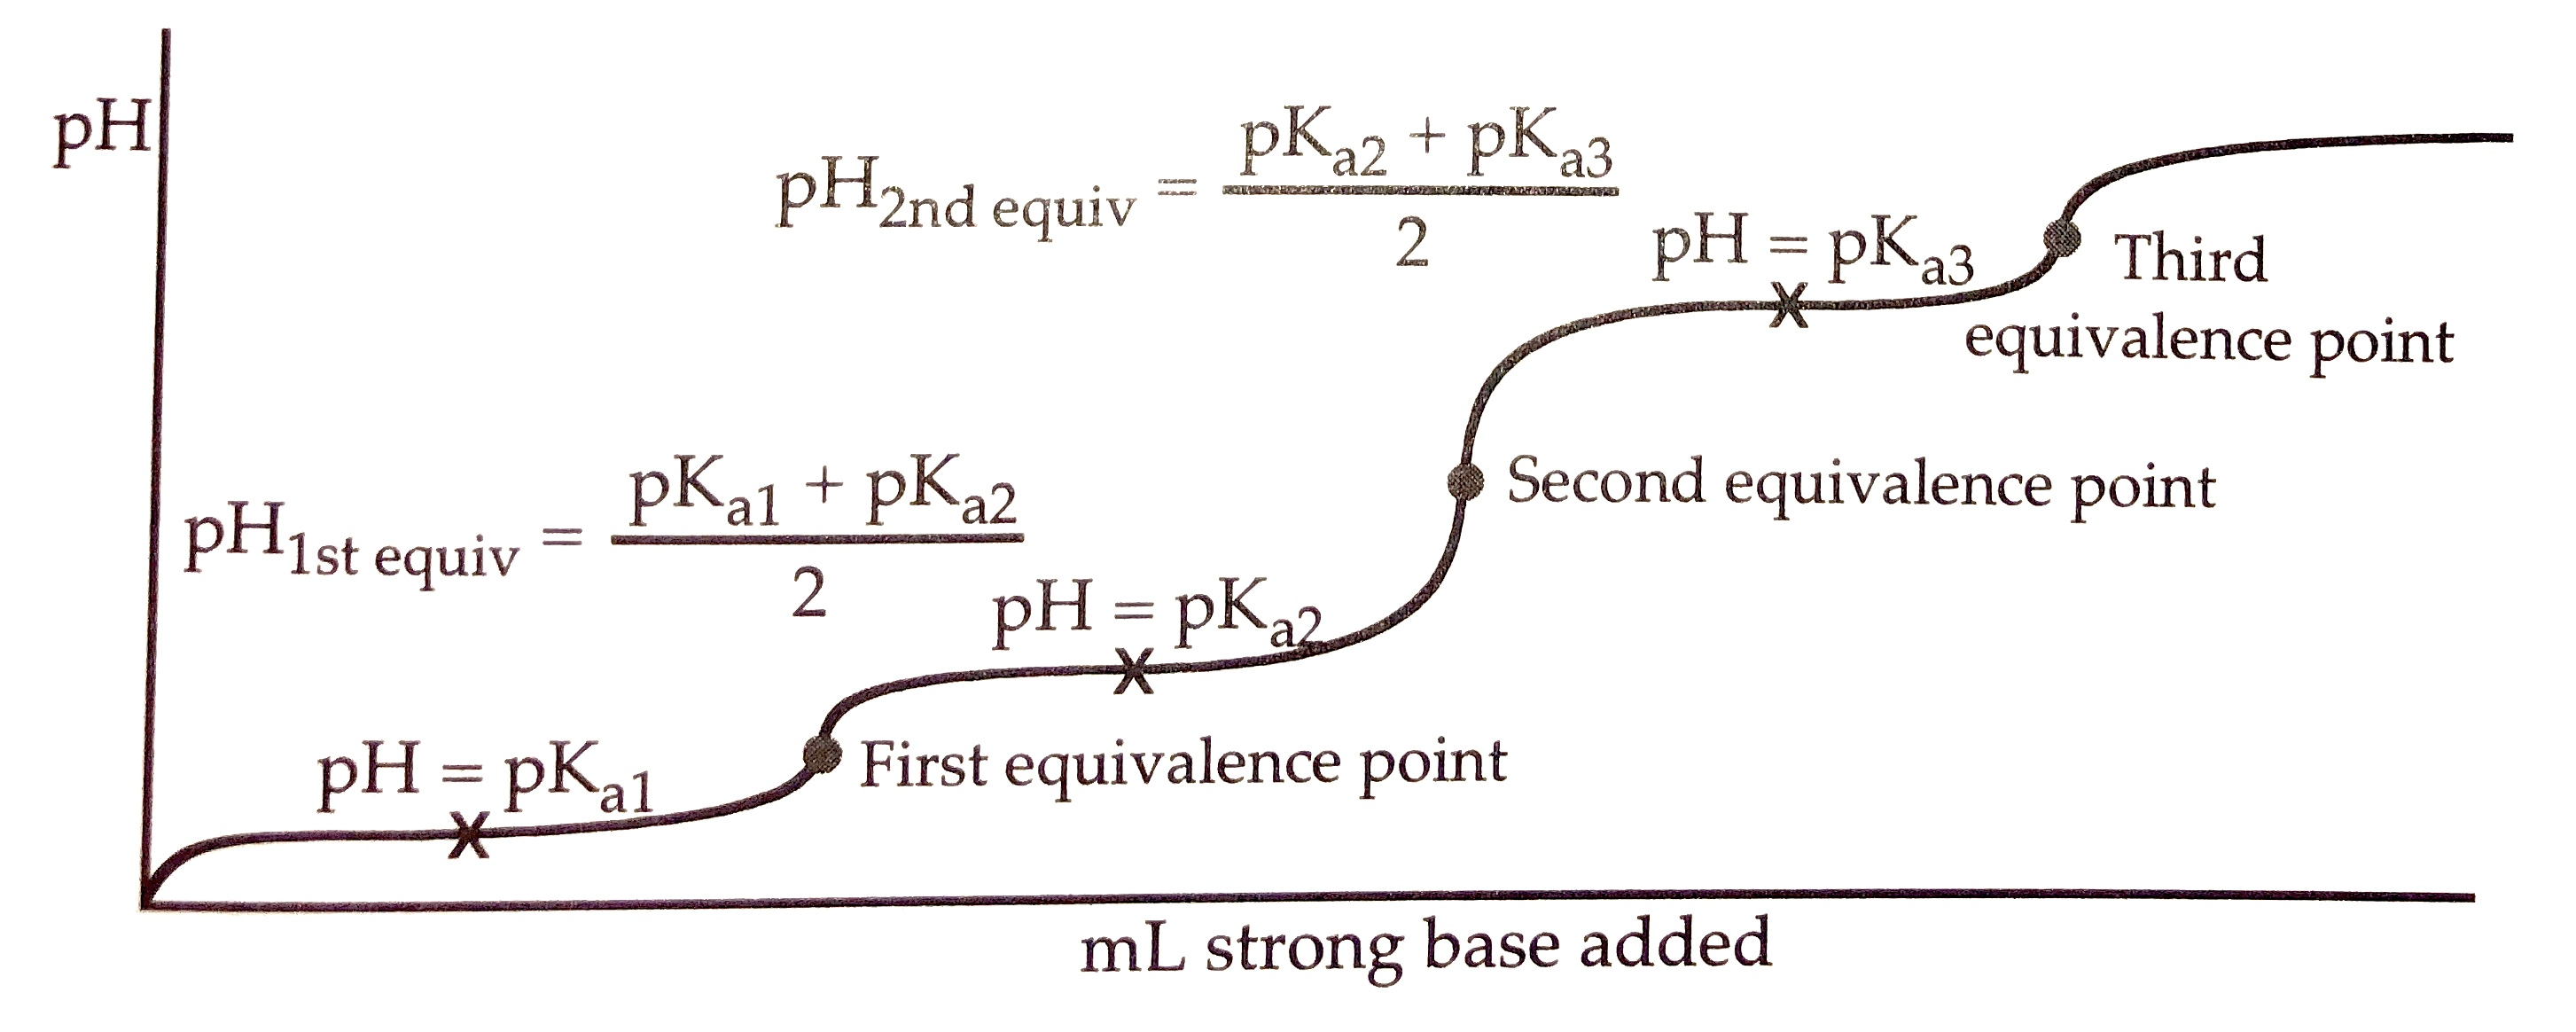
\includegraphics[width=0.7\textwidth]{polyprotic.png} \label{polyprotic}
\caption{An example of a titration curve with a polyprotic acid.}
\end{figure}
\indent A typical acid-base \textbf{indicator} is an organic acid with extended conjugation. Its weak acid and conjugate weak base have two distinct colors. The energy state transition that produces color involves the $\pi$-bonding and $\pi$-antibonding orbitals, and depends on the electron-donating and electron-withdrawing nature of the substituents on the $\pi$-system. An indicator is generally used for one of two purposes: the first is to detect the endpoint of a titration, and the second is to approximate the pH of a solution from the color of the indicator in the solution. The best scenario for an indicator detecting a titration endpoing is when the pH at equivalence equals the pK\textsubscript{a} of the indicator. The important fact to retain is that the pH at equivalence for the titration of a weak acid by a strong base can be approximated quite closely by averaging the pK\textsubscript{a} of the weak acid with the pH of the titrant strong base. For the titration of a weak base by a strong acid, the pH at equivalence can also be approximated by averaging the pK\textsubscript{a} of the conjugate acid of the weak base with the pH of the titrant strong acid.

\subsection{Equilibrium}
The \textbf{equilibrium constant} $K_{eq}$ is a mathematical quantity that is calculated for a reaction at equilibrium. By definition, the equilibrium constant is the concentration of products at equilibrium divided by the concentration of reactants at equilibrium. Stoichiometric values from the balanced equation become exponents in the $K_{eq}$ expression. Do \textit{not} include solids or pure liquids in the $K_{eq}$ expression, only solutes (for $K_c$) and gases (for $K_p$). The numerical value of $K_{eq}$ varies only with changing temperature, not with catalysts, pressure, volume, or moles. Equilibrium constants are unitless by definition. All equilibrium constants obey the same rules, but depending on the reaction, there may be special features that recur. Different reactions have special $K$ values.\\
\begin{table}[!ht]
\arraycolsep=1.4pt\def\arraystretch{1.5}
\begin{tabular}{|l|l|}
\hline
\textbf{$K$ Type}    & \textbf{Type of Reaction to Which the $K$ Applies} \\ \hline
$K_p$      & $K_{eq}$ for reaction of gases. Values are in \textit{pressure} units. \\ \hline
$K_c$       & $K_{eq}$ for reaction of solutes. Values are in \textit{concentration} units. \\ \hline
$K_{sp}$     & $K_{eq}$ for salts dissociating into ions. Measures the \textit{solubility}. \\ \hline
$K_{a}$   & $K_{eq}$ for acids dissociating into water. Measures the \textit{acidity}. \\ \hline
$K_{b}$    & $K_{eq}$ for bases dissociating in water. Measures the \textit{basicity}. \\ \hline
$K_w$     & $K_{eq}$ for autoionization of \textit{water} into \ce{H+} and \ce{OH-}. \\ \hline
\end{tabular}
\end{table}
\indent A \textbf{complex equilibrium} is a balance between two separate reactions that share a common reagent or set of reagents. In essence, it is two reactions who equilibrium states depend on one another. Here is an example of a complex equilibrium: 
\begin{center}
\begin{minipage}{30em}
\textcolor{blue}{Consider the following complex equilibrium. When \ce{N_2O_4} gas is removed, how are the partial pressures of \ce{NO} gas and \ce{NO_2} gas affected?
\begin{equation}
\begin{split}
\ce{2NO(g) + O_2(g) <-> 2NO_2(g)}, \quad K_{eq1}\\
\ce{2NO_2(g) <-> N_2O_4(g)}, \quad K_{eq2}\\
\hline\\
\ce{2NO(g) + O_2(g) <-> N_2O_4(g)}, \quad K_{eq1}\times K_{eq2}
\end{split}
\end{equation}
\begin{enumerate}[label=\Alph*]
	\item $P_{\ce{NO}}$ and $P_{\ce{NO_2}}$ both decrease.
	\item $P_{\ce{NO}}$ and $P_{\ce{NO_2}}$ both increase.
	\item $P_{\ce{NO}}$ decreases, while $P_{\ce{NO_2}}$ remains the same.
	\item $P_{\ce{NO}}$ increases, while $P_{\ce{NO_2}}$ remains the same.
\end{enumerate}}
\end{minipage}
\end{center}
\noindent The second reaction shifts to the right to compensate for the loss of \ce{N_2O_4}, so the partial pressure of \ce{NO_2} decreases. In turn, a decrease in \ce{NO_2} causes the first reaction to shift to the right as well, resulting in a decrease in the partial pressure of \ce{NO} gas and an increase in the partial pressure of \ce{NO_2}. However, this increase in \ce{NO_2} from the forward shift of the first reaction is less significant than the decrease in the \ce{NO_2} caused by the forward shift of the second reaction. This is because the shift in the first reaction cannot completely replenish the lost \ce{NO_2} without losing so much \ce{NO} that the reaction is beyond equilibrium. A shift \textit{never} regenerates as much as was lost. Both \ce{NO} and \ce{NO_2} this decrease, making choice \textbf{A} the best answer. \\
\indent Equilibrium is \textbf{dynamic}, meaning that it is a state where the system is continually reacting in both the forward and reverse directions, even though no net change is observed at the macroscopic level. \textbf{Le Ch\^atelier's Principle} says that if an external stress is applied to a system at equilibrium, the system will shift itself in such a way that the stress is partially relieved as best as possible and equilibrium is re-established. To see this in action, consider the reaction \ce{N_2O_4 <-> 2NO_2(g)}, which is an endothermic reaction with $\Delta H = +146$ kJ/mole:
\begin{enumerate}
	\item If \ce{N_2O_4(g)} is added, the system shifts to the right.
	\item If \ce{NO_2(g)} is added, the system shifts to the left.
	\item If the external pressure is increased, the system favors the side with less molecules to reduce the increased crowding, thus shifting the system to the left.
	\item If the volume is increased, the system is less crowded and molecules collide less often, so the system shifts to the right.
	\item If the system is heated, this gives a net influx of energy, shifting the \textit{endothermic} system to the right.
	\item If the system is cooled, the system wants to produce energy to compensate, shifting the system to the left.
\end{enumerate}

\subsection{Thermochemistry}
\textit{Exergonic} means $\Delta G<0$, while \textit{exothermic} means $\Delta H<0$. Similarly, \textit{Endogonic} means $\Delta G>0$, while \textit{endothermic} means $\Delta H>0$. The standard free energy change $\Delta G^{\circ}$ is the free energy change when a reaction goes from standard conditions to equilibrium. Standard conditions are defined as 1 atm of pressure and a temperature of 298 K, and all solute species (reactants and products) present at 1.00 M concentration. We have
\begin{equation}
\begin{split}
\Delta G^{\circ} = -RT\ln K_{eq}
\end{split}
\end{equation}
\noindent If we don't start at reaction quotient $Q=1$ by not having all the solute species at 1.00 M concentration, then the adjusted free energy change is
\begin{equation}
\begin{split}
\Delta G_{\text{rxn}}=RT\ln\frac{Q_{\text{rxn}}}{K_{eq}}
\end{split}
\end{equation}

\subsection{Chemical Kinetics}
The \textbf{order} of a reaction is ascertained from the number of reagents involved in the rate-determining step. There are three fundamental reaction orders to consider: zero, first, and second. 
\begin{table}[!ht]
\arraycolsep=1.4pt\def\arraystretch{1.5}
\begin{tabular}{|l|l|l|l|}
\hline
                      & \textbf{Zero Order} & \textbf{First Order} & \textbf{Second Order} \\ \hline
\textbf{Rate Law:}    & $\text{Rate}=k$                   & $\text{Rate}=k[A]$                    & $\text{Rate}=k[A]^2$                     \\ \hline
\textbf{Half-Life:}   & $t_{1/2}=\frac{[A]_0}{2k}$                   & $t_{1/2}=\frac{\ln 2}{k}=\frac{0.693}{k}$                    & $t_{1/2}=\frac{1}{k[A]_0}$                     \\ \hline
\textbf{Rate:} & Constant rate                   & Rate $\downarrow$ as time $\uparrow$              & Rate $\downarrow$ as time $\uparrow$                     \\ \hline
\textbf{Half-Life:} & Half-life $\downarrow$ as time $\uparrow$ & Half-life constant & Half-life $\downarrow$ as time $\downarrow$ \\ \hline
\end{tabular}
\end{table}
\indent The rate of a reaction is affected by several factors such as temperature, activation energy, catalysts, solvent (solvents affect the stability of the transition state), collision frequency, collision orientation, and the concentration of the reactants in the rate-determining step. The rate constant $k$ must account for all of these factors, except concentration of the reactants, and is given by
\begin{equation}
\begin{split}
k=A\exp\left(\frac{-E_{\text{activation}}}{RT}\right)
\end{split}
\end{equation}
\noindent where $A$ is the Arrhenius constant\textemdash it takes into account collision orientation and frequency. Because half-life is constant for first-order processes, most half-life questions on the MCAT involve decay (a first-order reaction), which can be described by
\begin{equation}
\begin{split}
C_t=C_0e^{-kt}
\end{split}
\end{equation}
\noindent where $C_t$ is the concentration at time $t$, $C_0$ is the initial concentration, $t$ is time, and $k$ is the rate constant. The half-life of decay is $t_{1/2}=\left(\ln 2\right)/k\approx 0.693/k$.\\
\indent In nuclear chemistry, a heavy element undergoes a decay process (i.e. fission) to increase its nuclear stability. A light element undergoes a capture process (i.e. fusion) when struck by a high-energy particle to increase its nuclear stability. 
\begin{table}[!ht]
\arraycolsep=1.4pt\def\arraystretch{1.5}
\begin{tabular}{|l|l|}
\hline
\textbf{Process}    & \textbf{Reaction Tracking} \\ \hline
$\alpha$-Decay      & \ce{{}^{120}_{50}X -> {}^{4}_{2}$\alpha$ + {}^{116}_{48}Y} \\ \hline
$\beta$-Decay       &  \ce{{}^{120}_{50}X -> {}^{0}_{-1}e + {}^{120}_{51}Z} \\ \hline
$\beta^+$-Decay     & \ce{{}^{120}_{50}X -> {}^{0}_{1}e + {}^{120}_{49}Q} \\ \hline
$\gamma$-Emission   & \ce{{}^{120}_{50}X^* -> h$\nu$ + {}^{120}_{50}X} \\ \hline
$\alpha$-Capture    & \ce{{}^{120}_{50}X + {}^{4}_{2}$\alpha$ -> {}^{124}_{52}A} \\ \hline
$\beta$-Capture     & \ce{{}^{120}_{50}X + {}^{0}_{-1}e -> {}^{120}_{49}Q} \\ \hline
$\beta^+$-Capture   & \ce{{}^{120}_{50}X + {}^{0}_{1}e -> {}^{120}_{51}Z} \\ \hline
$\gamma$-Absorption & \ce{{}^{120}_{50}X + h$\nu$ -> {}^{120}_{50}X^*} \\ \hline
\end{tabular}
\end{table}

\section{Organic Chemistry of Biological Systems}
\subsection{Molecular Structure}
For nonpolar $\sigma$ bonds, most of the electron density is \textit{between} the nuclei. This means that when drawing electron cloud diagrams, the $\sigma$ bond looks more like an ellipsoid as opposed to a dumbbell.\\
\indent The more substituted a carbon atom is, the less strong bonds it is able to form. This is because the other groups are able to (mildly) take electrons away from the bond of interest and thus make it weaker. Bonds involving $sp^3$ carbons are the weakest, while those involving $sp$ carbons are the strongest, because they have the most $s$ character. And of course, triple bonds are the strongest, while single bonds are the weakest, because of the number of electrons shared between atoms. For example, consider the molecule shown in Figure \ref{oc:1.4}.
\begin{equation}
\begin{split}
\chemfig{
           \mcfatomno{1}% 1
    -[:320]\mcfatomno{2}% 2
              (
        -[:260]\mcfatomno{13}% 13
                  (
            -[:320]\mcfatomno{15}% 15
                  )
        -[:200]\mcfatomno{14}% 14
              )
     =[:20]\mcfatomno{3}% 3
              (
         -[:80]\mcfatomno{5}% 5
              )
    -[:320]\mcfatomno{4}% 4
              (
        <[:260]H\mcfatomno{6}%\mcfright{H}{\mcfatomno{6}}% 6
              )
              (
       <:[:220]\mcfatomno{7}% 7
              )
     -[:10]\mcfatomno{8}% 8
              (
        <:[:60]H\mcfatomno{9}%\mcfright{H}{\mcfatomno{9}}% 9
              )
              (
      -[:287.5]\mcfatomno{11}% 11
              )
     <[:25]\mcfatomno{10}% 10
    -[:325]\mcfatomno{12}% 12
}
\end{split} \label{oc:1.4}
\end{equation}
Here, let us consider Bonds A (1 and 2), B (2 and 3), C (2 and 13), and D (4 and 8). Between these four bonds, B is the strongest since it is a double bond. D is the weakest because it is between two $sp^3$-hybridized carbons. Bond A is stronger than bond C, despite both sharing an $sp^2$-hybridized and $sp^3$ hybridized carbon, because bond C contains the more highly substituted carbon.\\
\indent Hybridization of carbon atoms can affect the acidity of hydrogens bound to them. Contrary to most other acids, as the hybrid orbital gets smaller, the electrons are held closer to the nucleus of the atom boned to hydrogen, so the bond can be cleaved in a heterolytic fashion more easily. The more $s$-character in the hybrid orbital of the atom bonded to the hydrogen, the stronger the acid. This results in the relative acidity being $sp>sp^2>sp^3$. This trend is most commonly observed with \ce{C} acidity, but can also be observed with \ce{N} and \ce{O}.\\
\indent Steric hindrance occurs any time two atoms attempt to be in the same place at the same time. It is repulsive in nature and increases as the atoms draw closer. On cyclohexane, substituents with axial orientation experience greater steric hindrance than substituents with equatorial orientation. Thus, substituents (especially the bulky ones) prefer to be in the equatorial position.\\
\indent \textit{Intermolecular forces are the primary consideration} when approximating physical properties (i.e. boiling point). If IMFs are not enough, you also need to consider the molecular mass and molecular rigidity of the molecules. Heavier compounds have higher boiling points, and compounds with greater molecular flexibility can twist and conform to allow for more surface area, and thus more intermolecular interactions. This is why cell membranes would be most rigid if their fatty acids were completely saturated and long molecules, as interactions are greatest with long, saturated fatty acids. \\
\indent The best micelles has an ionic (charged) head and a long carbon chain for the organic tail. For example, \ce{H_3C(CH_2)_{14}CO_2^-} is a better micelle than \ce{H_3C(CH_2)_{14}CO_2H} because it has a charged head, which is more hydrophilic than even the polar, protic carboxylic acid.\\
\indent The inductive effect can be applied to both electron withdrawal (i.e. with the canonical example of nearby halogens) and electron donation. For instance, methyl amine is more nucleophilic than ammonia (\ce{NH_3}) because the methyl group is electron-donating. Varying the $R$-group changes the inductive effect. It also changes the size of the molecule, so steric hindrance can affect the reaction. For instance, \ce{(H_3C)_3N} is less nucleophilic than \ce{(H_3C)_2NH} because the electron donation by the additional methyl group does not compensate for the increase in molecular size.\\
\indent Stereochemistry prefixes, to denote orientation:
\begin{itemize}
\item \textbf{R vs. S} R is clockwise around a stereocenter, S is counterclockwise. This convention is used for chiral centers.
\item \textbf{E vs. Z} E is high priority groups on opposite sides of the double bond. Z is high priority groups are on the same side of the double bond. This convention is used for double bonds.
\item \textbf{$\alpha$ vs $\beta$} $\alpha$ means that the hydroxyl group attached to \ce{C_1} (atom 8 in Figure \ref{oc:2} for both molecules) and the \ce{-CH_2OH} group at \ce{C_5} (the groups on atoms 2 and 10 in Figure \ref{oc:2} for both molecules) lies on opposite sides of the ring's plane (a \textit{trans} arrangement), while $\beta$ means that they are on the same side of the plane (a \textit{cis} arrangement). This convention is used when discussing the glycosidic bond between sugar molecules. 
\end{itemize}
\begin{equation}
\begin{split}
\chemfig{
            \mcfatomno{15}O% 15
    >:[:330]\mcfatomno{14}% 14
      -[:30]\mcfatomno{13}% 13
               (
          <[:90]O\mcfatomno{16}% 16
               )
     -[:330]\mcfatomno{12}% 12
               (
         <:[:30]O\mcfatomno{17}% 17
               )
     -[:270]O\mcfatomno{11}% 11
     -[:210]\mcfatomno{10}% 10
               (
        <:[:270]\mcfatomno{18}% 18
         -[:330]O\mcfatomno{19}% 19
               )
     -[:150]\mcfatomno{9}% 9
               (
          -[:90]\phantom{14}% -> 14
               )
     <[:210]O\mcfatomno{8}% 8
     >[:150]\mcfatomno{6}% 6
     -[:210]\mcfatomno{5}% 5
               (
        <:[:270]O\mcfatomno{20}% 20
               )
     -[:150]\mcfatomno{4}% 4
               (
         <[:210]\mcfatomno{21}O% 21
               )
      -[:90]\mcfatomno{3}% 3
               (
         <[:150]\mcfatomno{22}O% 22
               )
      -[:30]\mcfatomno{2}% 2
               (
         -[:330]O\mcfatomno{7}% 7
         -[:270]\phantom{6}% -> 6
               )
      <[:90]\mcfatomno{1}% 1
      -[:30]O\mcfatomno{23}% 23
} %lactose 
\quad
\chemfig{
            \mcfatomno{15}O% 15
    >:[:330]\mcfatomno{14}% 14
      -[:30]\mcfatomno{13}% 13
               (
          <[:90]O\mcfatomno{16}% 16
               )
     -[:330]\mcfatomno{12}% 12
               (
         <:[:30]O\mcfatomno{17}% 17
               )
     -[:270]O\mcfatomno{11}% 11
     -[:210]\mcfatomno{10}% 10
               (
        <:[:270]\mcfatomno{18}% 18
         -[:330]O\mcfatomno{19}% 19
               )
     -[:150]\mcfatomno{9}% 9
               (
          -[:90]\phantom{14}% -> 14
               )
     <[:210]O\mcfatomno{8}% 8
    >:[:150]\mcfatomno{6}% 6
     -[:210]\mcfatomno{5}% 5
               (
        <:[:270]O\mcfatomno{20}% 20
               )
     -[:150]\mcfatomno{4}% 4
               (
         <[:210]\mcfatomno{21}O% 21
               )
      -[:90]\mcfatomno{3}% 3
               (
        <:[:150]\mcfatomno{22}O% 22
               )
      -[:30]\mcfatomno{2}% 2
               (
         -[:330]O\mcfatomno{7}% 7
         -[:270]\phantom{6}% -> 6
               )
      <[:90]\mcfatomno{1}% 1
      -[:30]O\mcfatomno{23}% 23
} %maltose
\label{oc:2}
\end{split}
\end{equation}
\noindent The molecule on the left is lactose with a $\beta$ glycosidic bond, while the molecule on the right is maltose with an $\alpha$ glycosidic bond.\\
\indent The nitrogen atom in amides have planar geometry even if it doesn't appear like it! This is because of the resonance with the carbonyl oxygen group, as shown here:
\begin{equation}
\begin{split}
\begin{bmatrix}
\chemfig{
           O\mcfatomno{1}% 1
    =[:270]\mcfatomno{2}% 2
              (
        -[:330]{NH_2}\mcfatomno{3}% 3
              )
    -[:210]\mcfatomno{4}H% 4
}
\quad\begin{matrix}
\\
\\
\text{\ce{<=>}}
\end{matrix}\quad
\chemfig{
           {O^-}\mcfatomno{1}% 1
    -[:270]\mcfatomno{2}% 2
              (
        =[:330]{NH_2^+}\mcfatomno{3}% 3
              )
    -[:210]\mcfatomno{4}H% 4
}
\end{bmatrix}
\end{split}
\end{equation}
\noindent In this case, we can see that due to resonance, all of the atoms are coplanar for the amide. Quite separately, consider the following example problem:
\begin{center}
\begin{minipage}{30em}
\textcolor{blue}{20. \quad The STRONGEST hydrogen bond is formed between:
\begin{enumerate}[label=\Alph*]
	\item the lone pair of O and a hydrogen bonded to O.
	\item the lone pair of N and a hydrogen bonded to O.
	\item the lone pair of O and a hydrogen bonded to N.
	\item the lone pair of N and a hydrogen bonded to N.
\end{enumerate}}
\end{minipage}
\end{center}
\noindent The answer to this question is answer choice B. This is because the strongest hydrogen bond is formed when the hydrogen is extremely electron deficient (i.e. through being bonded to an oxygen) and it is hydrogen-bonded to something that is extremely basic (or in other words, is very good at donating its electrons in order to create the bond, which best describes the lone pair on a nitrogen atom). \\
\normalsize

\subsection{Isomers and Stereochemistry}
Isomers can be constitutional/structural (meaning they differ in connectivity of bonds) or stereoisomers (meaning they differ in the spatial arrangement of the atoms). Stereoisomers can either be conformers or configurational isomers. Conformers can differ by orientation in space, and are identical after a specific rotation about a $\sigma$-bond. Configurational isomers also differ by orientation in space, but you can't rotate them to become identical. Configurational isomers can be categorized as either enantiomers or diastereomers. \textbf{Enantiomers} are nonsuperimposable mirror images, while \textbf{diastereomers} are nonsuperimposable structures that are not mirror images. Configurational isomers can also be categorized as either optical isomers or geometrical isomers. \textbf{Optical isomers} rotate plane-polarized light and cannot be rotated to become identical due to the asymmetry in the structure, while \textbf{geometrical isomers} are structures with limited rotation, and can't be rotated to become identical due to the presence of a ring or $\pi$-bond. Geometrical isomers are sometimes also called \textit{cis/trans} isomers. The two categorizations are not mutually exclusive. \\
\indent The Chan-Ingold-Prelog Rules are used to determine the \textbf{absolute configuration} ($R$ vs. $S$) for a stereocenter. The rules are as follows:
\begin{enumerate}
	\item First, you must prioritize the substituents that are attached to the carbon of the stereocenter according to the atomic mass of the atom directly bonded to the chiral carbon (from heaviest atom to lightest atom).
	\item Next, orient the molecule in such a way that the substitutent with the lowest priority points behind the plane of the molecule.
	\item Finally, draw a semicircular arc from substituent 1 through substituent 2 and on to substituent 3. If the arc is clockwise, then the stereocenter is referred to as $R$. If the arc is counterclockwise, then the stereocenter is referred to as $S$. 
\end{enumerate}
\noindent Optical rotation is a characteristic feature of enantiomers that are described by absolute configurations. If, say, the $R$-enantiomer of a compound rotates the light in a positive direction (meaning clockwise) by $X$ degrees, then the $S$-enantiomer of the compound rotates light by $X$ degrees in the negative direction. However, in actuality, the $R$-enantiomer doesn't always rotate light in the positive direction\textemdash it really depends on the identity of the compound of interest.\\
\indent For compounds with multiple chiral centers, here is another way of thinking about enantiomers vs. diastereomers:
\begin{enumerate}
	\item \textbf{Enantiomers} are configurational isomers in which \textit{all} of the chiral centers in each molecule are different from one another.
	\item \textbf{Diastereomers} are configurational isomers in which \textit{at least one, but not all} of the chiral centers in each molecule is different from one another. 
\end{enumerate}
\indent For \textit{geometrical isomers}, which have different spatial arrangements about a $\pi$-bond, the prefix of E is given for trans orientation of the two highest priority groups, while Z is given for cis orientation of the two highest priority groups. \\
\indent \textbf{Meso compounds} are individual structures which contain a mirror plane slicing through the middle of the compound and an \textit{even number} of chiral centers symmetrically displaced about the mirror plane. The net optical rotation of a meso compound is 0 degrees because the opposing chiral centers on each half of the molecule cancel one another out, leaving no net rotation of plane polarized light. A meso compound may be identified by either an inversion center in the middle of the molecule, or a mirror plane through the middle of the molecule.\\
\indent When a molecule contains more than one chiral center, the maximum number of stereoisomers increases exponentially with each new chiral center according to the equation
\begin{equation}
\begin{split}
\text{Number of stereoisomers}=2^n
\end{split}
\end{equation}
\noindent where $n$ is the number of chiral carbons in the molecule. There are less than $2^n$ stereoisomers if one of the possible structures is meso. If $n$ is odd, however, there can't be a meso compound, meaning that there must be exactly $2^n$ stereoisomers.\\
\indent Rotational about $\sigma$ bonds allows for different conformers. The two extreme overall structures are known as \textit{staggered} (where substituents on the first atom do not block the substituents on the back atom of the $\sigma$ bond in question) and \textit{eclipsed} (where substituents on the first atom do block the substituents on the back atom of the $\sigma$ bond in question). Within staggered conformation, the terms \textit{gauche} and \textit{anti} describe the relative position of substituents on adjacent atoms. \textit{Gauche} conformers have the two groups of interest (often the largest groups) having a dihedral angel of 60 degrees, while \textit{anti} conformers have the two groups of interest having a dihedral angle of 180 degrees. Staggered and anti is the most stable, because steric repulsion is minimized. To understand these different types of conformers, take a look at the Newman projections shown in Figure \ref{conformers}.\\
\begin{figure}[!ht]
\centering
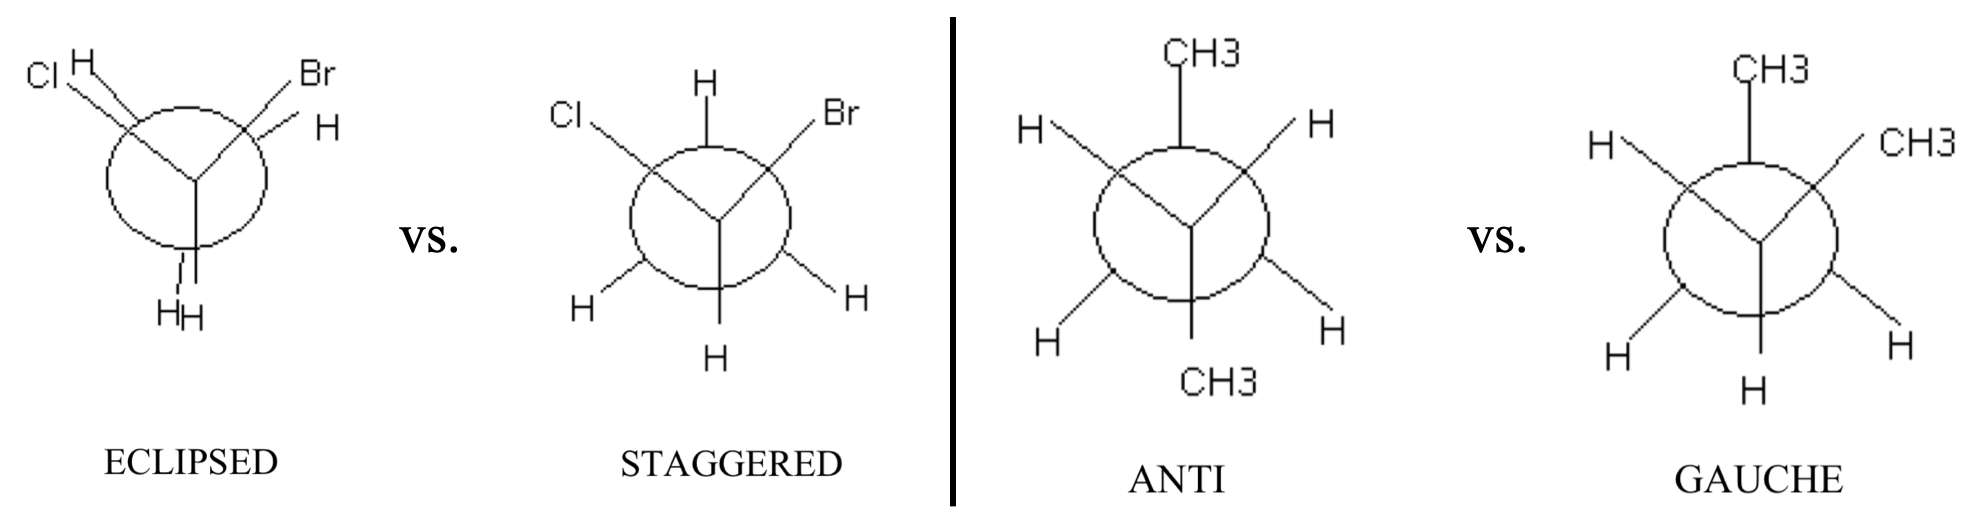
\includegraphics[width=0.6\textwidth]{conformers.png} \label{conformers}
\caption{\textit{Left} Staggered vs. eclipsed conformers. \textit{Right} Staggered conformers can be either gauche or anti.}
\end{figure}
\indent Cycloalkanes are basically cyclic alkanes that have one ring with the chemical formula \ce{C_nH_{2n}} and contain no $\pi$-bonds. Three- and four- membered rings are reactive, while five- and six- membered rings are stable. The reactivity of tree- and four- membered rings is attributed to \textit{ring strain}, defined as the energy difference between the linear and cyclic alkanes of equal carbon length. Let's look at a couple of particularly important cycloalkanes:
\begin{itemize}
	\item Cyclopentane does not require much distortion of its bonds and shape to accommodate the $109.5^{\circ}$ angle for the $sp^3$ hybrid. To achieve the correct angle and alleviate the torsional strain, cyclopentane forms an \textit{envelope shape} where one of the carbons is not coplanar with the other four. However, even with this envelope shape, the substituents on the ring that are in an eclipsed conformation as a result of the near-planar ring structure are unfavorable, causing further contortion of the structure, which accounts for the ring strain energy.  The envelope conformation is shown in \textbf{Fig. \ref{chairs}}.
	\item Cyclohexane has the most stable ring structure of all of the cycloalkanes. The most stable form is the \textit{chair} conformation. Cyclohexane can flip between different chair conformations in a process called \textit{ring-flipping}, and the interconversion process requires that it passes through the \textit{boat} conformation. Equatorial positions (in the plane of the molecule) are more stable than axial (above and below the plane of the molecule), so the most stable conformation of a cyclohexane compound has the largest substituents in the equatorial positions. The chair conformation of cyclohexane is shown in \textbf{Fig. \ref{chairs}}.
\end{itemize}
\begin{figure}[!ht]
\centering
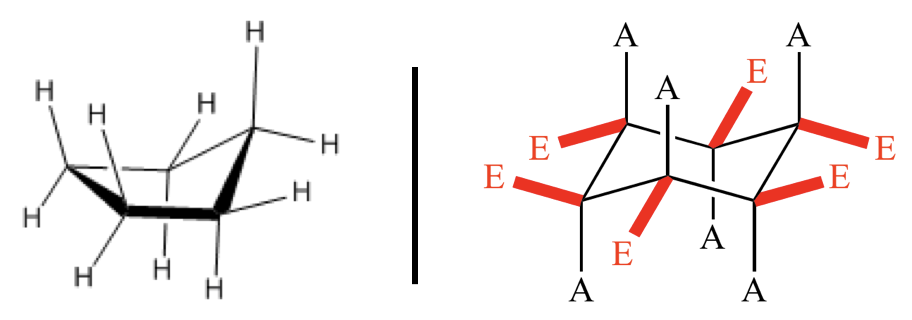
\includegraphics[width=0.5\textwidth]{chairs.png} \label{chairs}
\caption{\textit{Left} Envelope shape of cyclopentane. \textit{Right} Axial (A) and equatorial (E) positions in cyclohexane chair conformation.}
\end{figure}
\indent \textbf{Separating Stereoisomers:} In organic chemistry, there are compounds known as \textit{chiral auxiliaries}, which introduce chirality to, or exaggerate existing chirality within, a reactant molecule. Chiral auxiliaries serve in a similar fashion to an enzyme. When aiming for one specific stereoisomer, it is easiest to select for it in the reaction. If not, then a mixture of stereoisomers forms and chirally selective separation techniques must be used. Chirally selective separation techniques come in two types: using an enzyme/chirally selective molecule to react specifically with one stereoisomer within the mixture, or invoking chirality in an existing separation technique. As an example for the first technique, if a new functional group is added to only stereoisomer by an enzyme, the two enantiomers now have different physical properties and can easily be separated. Once separated, the same enzyme can be employed to return the compound back to its original form. As an example for the second technique, a column chromatography gel can be made from a pure stereoisomer. If the column is made with an $R$-alcohol for instance, then when a racemic mixture of alcohols is added, the $S$-enantiomer has a greater affinity for the column, and thus has a greater elution time.

\subsection{Nucleophilic Substitution}
The strength of a leaving group can be predicted by the \ce{pK_a} os its conjugate acid. The more stable the leaving group, the less basic the leaving group, and thus the more acidic the conjugate acid of the leaving group. In other words, the strength of a leaving group increases as the \ce{pK_a} of its conjugate acid decreases.\\
\indent A \textit{racemic mixture} is a product mixture that has an even distribution of enantiomers. It is the observed product when the mechanism involves an intermediate where the reactive site is an $sp^2$-hybridized carbon and the molecule is symmetric (i.e. has no other chiral centers). \\
\indent \ce{S_N 2} reactions involve the nucleophile attacking prior to the leaving group leaving in a \textit{backside} attack, essentially pushing the leaving group off of the electrophile. It has a trigonal bipyramidal transition state.
\begin{table}[!ht]
\begin{tabular}{p{6.25cm} p{6.5cm} p{5cm}}
\hline
\textbf{Reactant Features} & \textbf{Course of Reaction Features} & \textbf{Product Features} \\
\hline
\hline
The reactivity preference in an \ce{S_N 2} mechanism is $1^{\circ}>2^{\circ}>3^{\circ}$ in terms of electrophiles. & An \ce{S_N 2} mechanism forms a five-ligand transition state during the middle of the reaction. & A single enantiomeric product is formed (i.e. no racemic mixture). \\
An \ce{S_N 2} mechanism is favored with a good nucleophile. & The 5-ligand transition state is the highest energy state and it exists for just a split second. It \textit{cannot} be isolated. & \ce{S_N 2} reactions exhibit second order kinetics. \\
An \ce{S_N 2} mechanism is favored in polar, aprotic solvents such as ethers and ketones. & Steric forces destabilize the transition state by forcing bond angles to values less than $109.5^{\circ}$. & \ce{S_N 2} reactions are one-step reactions, so they have fast rates of formation.\\
\hline
\end{tabular}
\end{table}
\indent \ce{S_N 1} reactions involve the leaving group leaving before the nucleophile attacks. The carbocation intermediate has a long enough lifetime to be detected using spectroscopy. Both rearrangement (e.g. hydride shifts and alkyl shifts) and a mixture of stereoisomers (formed from either front-side or back-side attack of the $sp^2$-intermediate) are observed with \ce{S_N 1} reactions. Formation of the carbocation is the rate-limiting step. \\
\begin{table}[!ht]
\begin{tabular}{p{6.25cm} p{6.5cm} p{5cm}}
\hline
\textbf{Reactant Features} & \textbf{Course of Reaction Features} & \textbf{Product Features} \\
\hline
\hline
The reactivity preference in an \ce{S_N 1} mechanism is $3^{\circ}>2^{\circ}>1^{\circ}$ in terms of electrophiles. & Steric hindrance pushes the leaving group off of the electrophile. & A racemic mixture forms when the electrophile has chirality. \\
An \ce{S_N 1} mechanism is seen with a poor nucleophile. & The intermediate is a planar, three-ligand carbocation where the carbon has $sp^2$-hybridization. & \ce{S_N 1} reactions exhibit first order kinetics. \\
An \ce{S_N 1} mechanism is favored in protic solvent such as alcohols. & An intermediate is observed in addition to transition states. & \ce{S_N 1} reactions are slow, two-step reactions.\\
\hline
\end{tabular}
\end{table}
\indent The \ce{S_N 1} reaction can be complicated by \textbf{rearrangement} because of the carbocation intermediate formed. If a secondary carbocation (\ce{R_2CH^+}) is formed, it can rearrange to form a more stable tertiary carbocation (\ce{R_2C^+}) when possible. See Figure \ref{1-2-hydride-shift-mechanism} for an example. Furthermore, if the electrophile has a chiral center at a site other than the electrophilic carbon, an \ce{S_N 1} reaction will form both a major and minor product. The major product results from the transition state with least steric hindrance.
\begin{figure}[!ht]
\centering
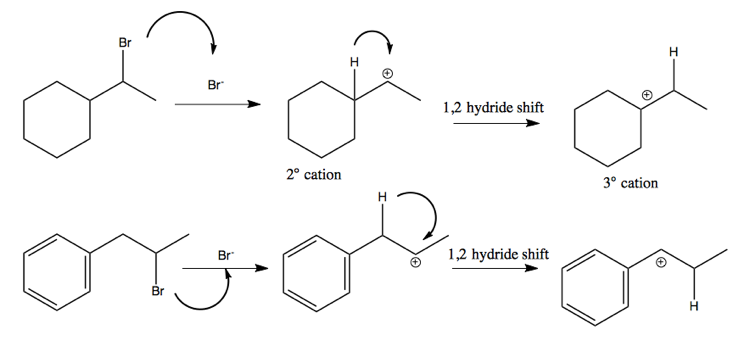
\includegraphics[width=0.7\textwidth]{1-2-hydride-shift-mechanism.png} \label{1-2-hydride-shift-mechanism}
\caption{Example of favorable hydride shift to generate tertiary carbocation from secondary carbocation intermediate.}
\end{figure}
\noindent Primary electrophiles proceed by \ce{S_N 2} while tertiary electrophiles proceed by \ce{S_N 1}. Secondary electrophiles can proceed by either \ce{S_N 1} or \ce{S_N 2}. Also, the stronger the nucleophile, the more likely the reaction will proceed by an \ce{S_N 2} mechanism; the better the leaving group, the more likely the reaction will proceed by an \ce{S_N 1} mechanism. Also, consider the following rate laws:
\begin{equation}
\begin{split}
\ce{S_N 1} \text{ Rate}=k\left[\text{Electrophile}\right]\\
\ce{S_N 2} \text{ Rate}=k\left[\text{Nucleophile}\right]\left[\text{Electrophile}\right]
\end{split}
\end{equation}
\noindent Lastly, you can also consider the solvent to distinguish between \ce{S_N 1} and \ce{S_N 2} reactions: if the solvent is protic (i.e. capable of forming hydrogen bonds), the reaction will have a tendency to proceed by an \ce{S_N 1} mechanism. If the solvent is aprotic (i.e. \textit{not} capable of forming hydrogen bonds), the reaction will have a tendency to proceed by an \ce{S_N 2} mechanism.

\subsection{Structure Elucidation}
When deducing the molecular structure for an organic molecule, it helps to know something about the symmetry of the compound and its units of unsaturation. The equation for units of saturation:
\begin{equation}
\begin{split}
\text{Units of Unsaturation} = \frac{2(\#C)+(\#N)-(\#H)-(\#X)+2}{2}
\end{split}
\end{equation}
\noindent In terms of spectroscopy, the MCAT includes infrared (IR) absorption spectroscopy, ultraviolet-visible spectroscopy, \ce{{}^1H} NMR spectroscopy, and mass spectroscopy. We will discuss all of these.\\
\indent \large\textbf{Infrared Spectroscopy:} \normalsize Infrared spectroscopy starts by adding a monoshromatic beam of IR photons to either a thin oil suspension (if the compound is a solid) or a neat solution (if the compound is a liquid) between salt plates. The molecule absorbs electromagnetic radiation that causes transitions between \textit{vibrational energy} levels within it. Vibrational potential energy is described by the equation $\text{PE}=\frac{1}{2}kx^2$; we can say the spring constant $k$ describes the bond strength, and the displacement $x$ describes the distance from equilibrium that the bond has stretched. This means stronger bonds absorb at higher wavenumbers; this can be accomplished by either having multiple bonds or by bonding to an $sp^2$ carbon instead of an $sp^3$ carbon, among other ways. IR spectroscopy is used as a diagnostic tool to detect certain functional groups.\\
\indent Hydrogen bonding results in a broadened peak, observed in both the IR and NMR techniques. In the case of IR, the broadening of the \ce{- OH} absorbance associated with hydrogen-bonding is caused by the weakening of the covalent bond between the hydrogen and the atom (nitrogen, oxygen, or fluorine) to which it is bonded. This lowers the energy of the covalent bond and thus lowers the energy of absorption for the bond. As the hydrogen bond increases in strength, the covalent bond weakens. \\
\indent \large\textbf{Ultraviolet-Visible Spectroscopy:} \normalsize While infrared photons affect the vibrational energies of a molecule, ultraviolet and visible photons affect the electronic energy levels. Because $\sigma$-bonds are so much stronger than $\pi$-bonds, the lowest energy absorbance for alkanes is significantly higher than the lowest energy absorbance for alkenes. As a result, we typically use UV-visible spectroscopy to analyze molecules with $\pi$-bonds, especially conjugated systems. UV-visible spectroscopy focuses on transitions between the $\pi$ and $\pi^*$ energy levels. For systems with conjugation, there are several $\pi$-levels, but we care about only the lowest energy transition. \\
\indent The transition of interest is from $\pi$ to $\pi^*$. The wavelength of highest absorbance, known as $\lambda_{max}$, changes with the amount of conjugation. As the amount of conjugation increases, so does $\lambda_{max}$. This is depicted in \textbf{Fig. \ref{conjugation}}. Color results from excessive conjugation within a molecule. Conjugated aldehydes and ketones have about the same $\pi$-$\pi^*$ absorbances as conjugated alkenes of the same number of $\pi$-bonds. However, conjugated aldehydes and ketones have other, more intense absorbances that are of longer wavelength than their hydrocarbon counterparts. This is attributed to the $n$-to-$\pi^*$ transition associated with aldehydes and ketones, possible because of the lone pair of electrons on the carbonyl oxygen. \\
\indent Unlike IR spectroscopy, UV-visible spectroscopy can be applied in a quantitative fashion, and can be used to determine the yield of a reaction, if it involves a UV-visible active compound. \\
\begin{figure}[!ht]
\centering
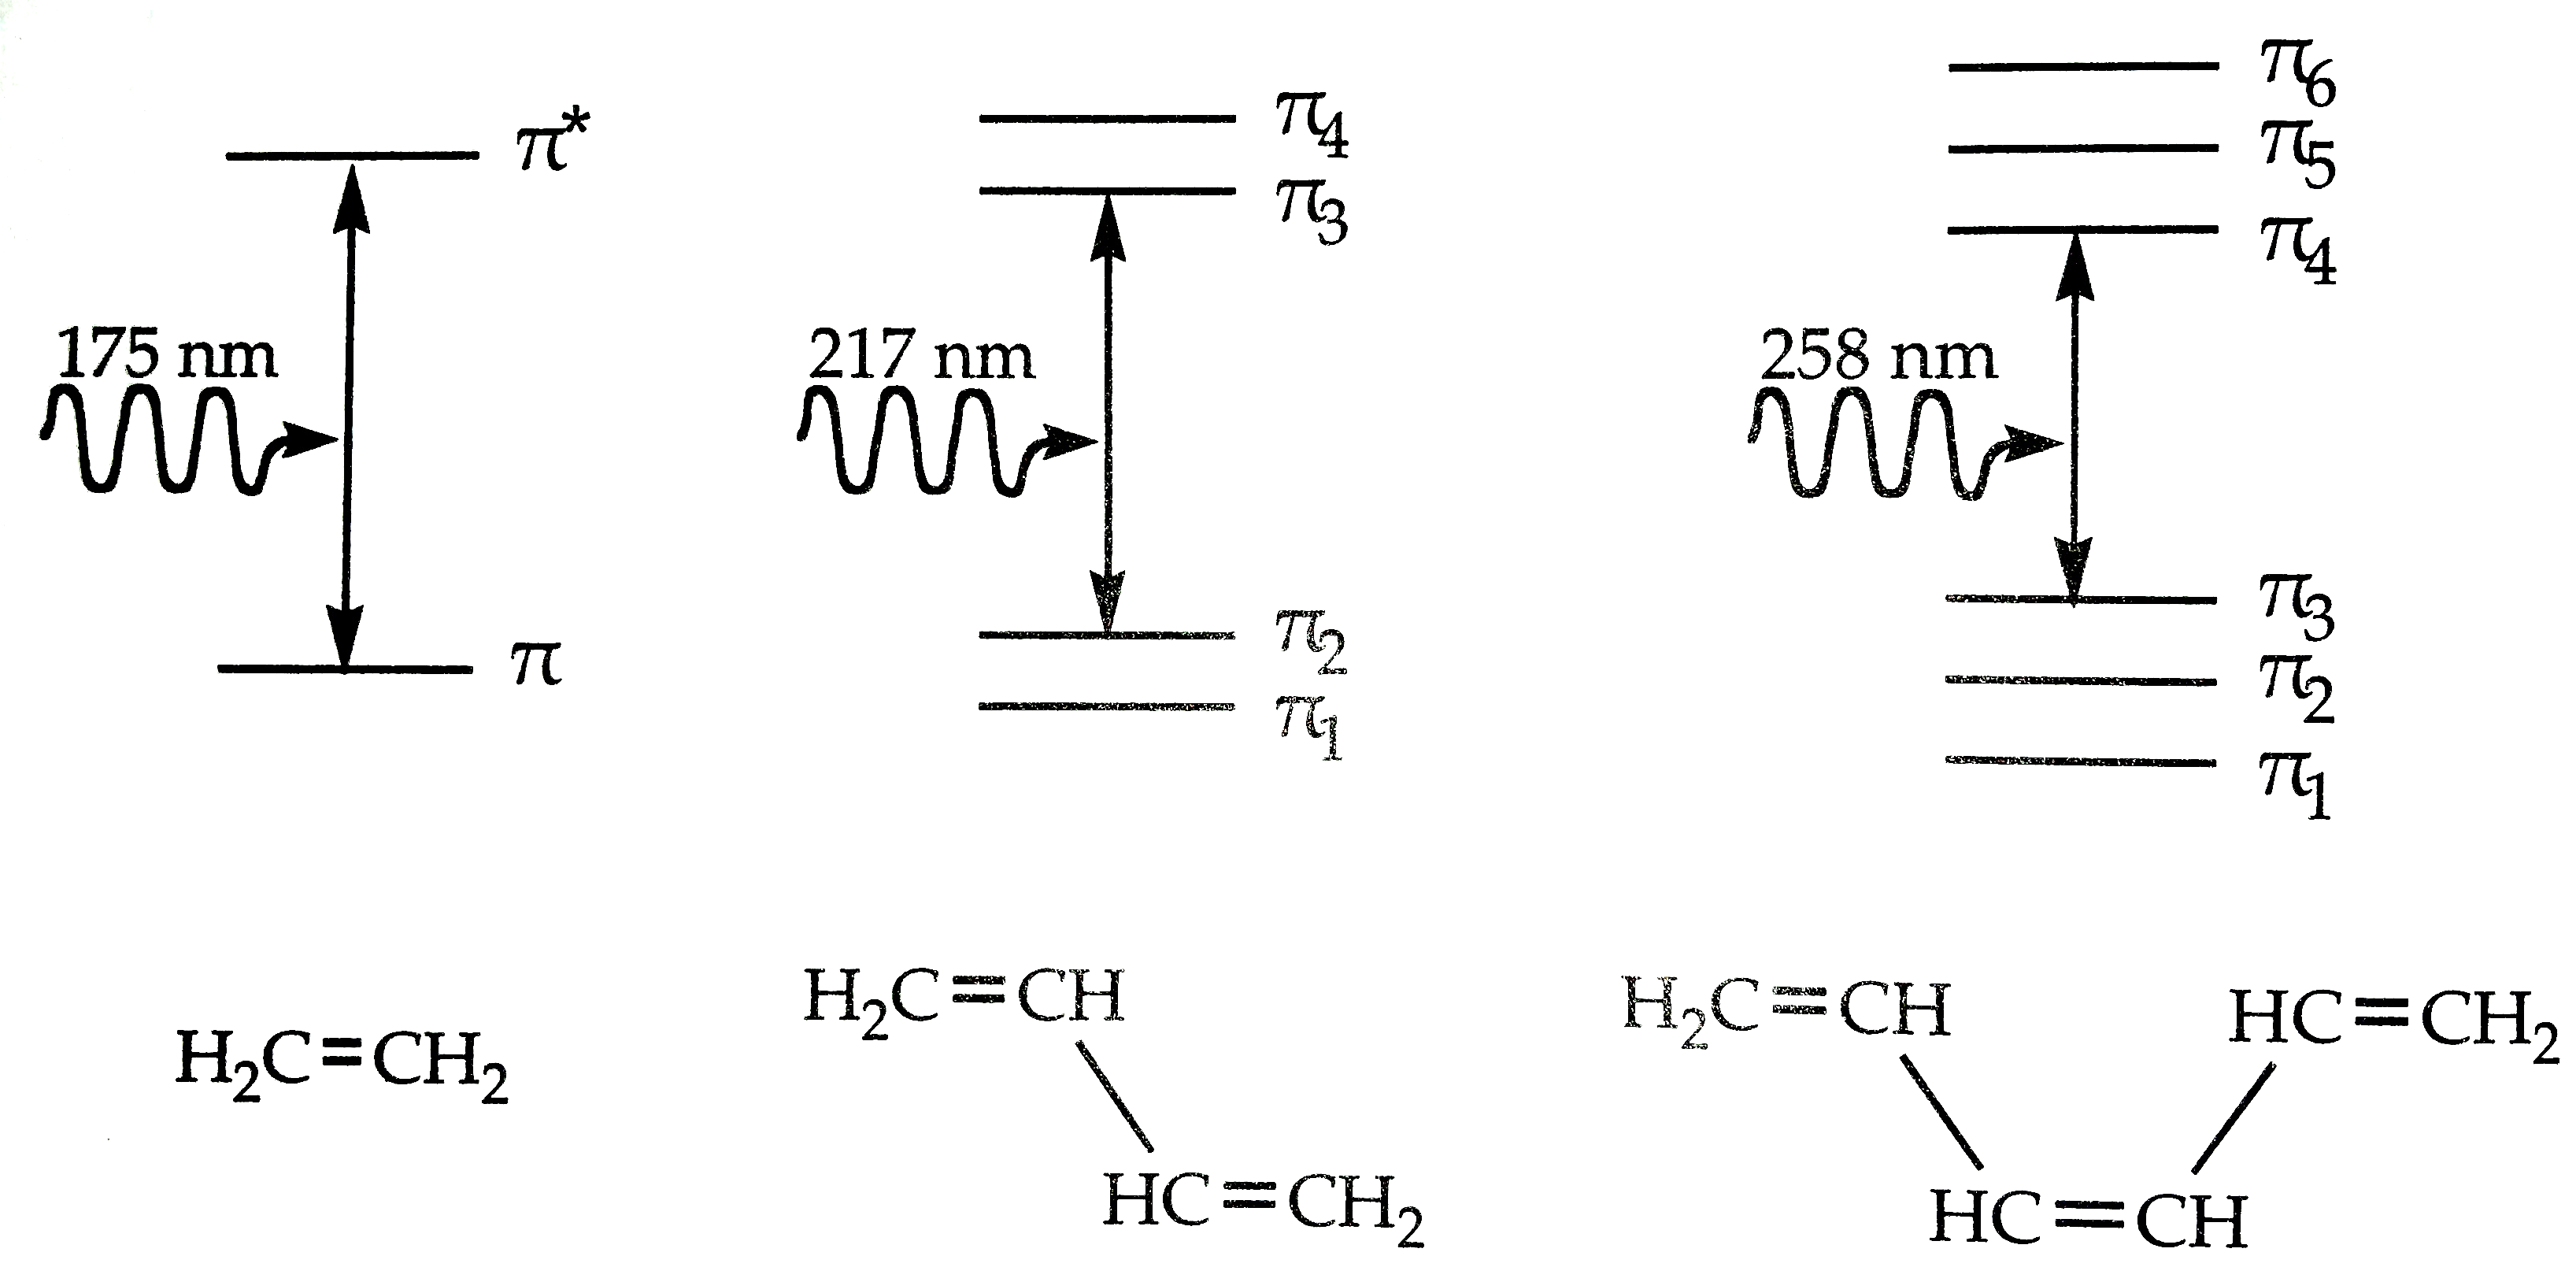
\includegraphics[width=0.7\textwidth]{conjugation.png} \label{conjugation}
\caption{Comparing the wavelengths of highest absorbance for different molecules of varying degrees of conjugation.}
\end{figure}
\indent \large\textbf{Nuclear Magnetic Resonance:} \normalsize Normally, all of the nuclei have spins of the same energy. However, when an external magnetic field is applied, spins can either align with the field or align against the field, so multiple energy states are possible. In the case of \ce{{}^1H}, there are two energy levels: $\alpha$ (the one aligned with the external magnetic field) and $\beta$ (the one antialigned with the external magnetic field). The $\beta$ energy level is defined as higher than the $\alpha$ energy levels. The energies of the two levels depend on the strength of the external magnetic field and the magnetogyric ratio of a particular nucleus. \\
\indent Any nucleus with an odd number of protons or an odd number of nucleons has a net spin. `Spin' is just that as the nucleus precesses, it generates a weak magnetic field. In the absence of any surrounding electrons, all identical nuclei exhibit the same spin and therefore require the same energy for excitation in an external magnetic field. Within a molecules, however, two identical nuclei may be in different electronic environments. As a result of the difference in their local magnetic fields, caused by the moving electrons, they do not require exactly the same amount of energy to excite the nucleus to a higher-energy spin state. \ce{{}^1H} NMR shift values are listed relative to a standard compound, tetramethylsilane (\ce{(H_3C)_4Si}). All twelve hydrogen atoms on tetramethylsilane are equivalent, so they absorb at the same value. \\
\indent The best place to begin NMR for the MCAT is with molecular symmetry. Based on the symmetry of a molecule, you can determine the number of equivalent hydrogens that it contains. The number of different hydrogens in the molecule corresponds to the number of different peaks on the NMR graph. The number of hydrogens that are the same is also correlated with the peak intensity/height on the NMR graph. \\
\indent In the case of alcohols, such as butanol, the protic hydrogen can be distinguished from other signals by its broadness. Broadening results from hydrogen-bonding in solution. Hence, alcohols are easily distinguished from ethers by the presence of a broad peak in their \ce{{}^1H} NMR spectrum. \\
\indent The three basic components of an NMR graph are the integral, splitting pattern, and shift value. The \textit{integral} is determined by the number of hydrogens making up a signal. The \textit{splitting pattern} is derived from the coupling between hydrogen on adjacent neighboring atoms. The splitting pattern is also referred to as \textit{coupling}. The \textit{shift value} is determined by the local magnetic field caused by either lone pair electrons in motion or the electronic density associated with electronegative atoms. \\
\indent Let's talk a bit more about splitting. Like electrons, nuclear particles have spin that can be classified as either up or down. The magnetic field resulting from the nuclear spin of hydrogen can be felt by the hydrogens on a neighboring atom. Because the spin can be either of two ways, the magnetic field may be additive or subtractive. The number of splitting peaks is equal to the number of equivalent hydrogens on the adjacent atoms plus one. The ratio of intensities of the peaks can be determined through binomial expansion (e.g. a quartet has a ratio of 1:3:3:1). \\
\indent The shift value is used to assess the local electronic environment around a hydrogen. It is measured in parts per million (ppm) relative to the magnetic field necessary to detect H's on a standard compound, tetramethylsilane. Shift values tell us what functional groups are present. Deshielding effects require a stronger external magnetic field to energize the spin levels. The more deshielded a proton's environment is, the more \textit{downfield} it is with a greater ppm.\\
\begin{table}[!ht]
\begin{tabular}{| l | l || l | l |}
\hline
\textbf{Hydrogen Atom} & \textbf{$\delta$ (ppm)} & \textbf{Hydrogen Atom} & \textbf{$\delta$ (ppm)} \\ \hline
RC\textbf{H}\textsubscript{3} & 0.8-1.0 & RC\textbf{H}\ce{=}CR\textsubscript{2} & 5.2-6.4 \\
RC\textbf{H}\textsubscript{2}R & 1.3-1.8 & RN\textbf{H}\textsubscript{2} & 1-3 \\
RCOC\textbf{H}\textsubscript{3} (ketone) & 2.1-2.5 & RNHC\textbf{H}\textsubscript{3} & 2.0-3.2 \\
RC\ce{#}C\textbf{H} & 2.5-2.6  & RO\textbf{H} (alcohol) & 1-5 (broad) \\
ROC\textbf{H}\textsubscript{3} (ether) & 3.5-4.0 & Ar\textbf{H} (benzene) & 7.0-7.4 \\
RC\textbf{H}\textsubscript{2}X (X=\ce{Cl}, \ce{Br}, \ce{I}) & 3.0-3.8 & RCO\textbf{H} (aldehyde) & 9.0-9.8 \\
RCO\textsubscript{2}C\textbf{H}\textsubscript{3} (ester) & 3.5-4.0 & RCO\textsubscript{2}\textbf{H} (acid) & 10-12 (broad) \\\hline
\end{tabular}
\end{table}
\indent Be aware of certain peaks and features that occur over and over. For instance, whenever you see a triplet and quartet in a 3:2 ratio, you should conclude that there is an isolated ethyl group (\ce{H_3CCH_2 -}) in the molecule somewhere. Whenever you see a doublet and a septet in a 6:1 ratio, you should conclude that there is an isolated isopropyl group \ce{(H_3C)_2CH -} somewhere in the molecule. \\
\indent \textbf{Distinguishing Disubstituted Benzenes:} Integrals tell us the number of equivalent hydrogens in a signal and are often employed to determine the position of substituents on disubstituted benzene rings. Structures that are highly symmetrical have more equivalent hydrogens than asymmetrical structures. \textbf{Fig. \ref{benzene_nmr}} shows the expected patterns on disubstituted benzene rings depending on if they are ortho-, meta-, or para- substituted. Para substitution is the easiest arrangement to distinguish of the three possible structural isomers, because it has a doublet of doublets. Para coupling is a highly recognizable feature.\\
\begin{figure}[!ht]
\centering
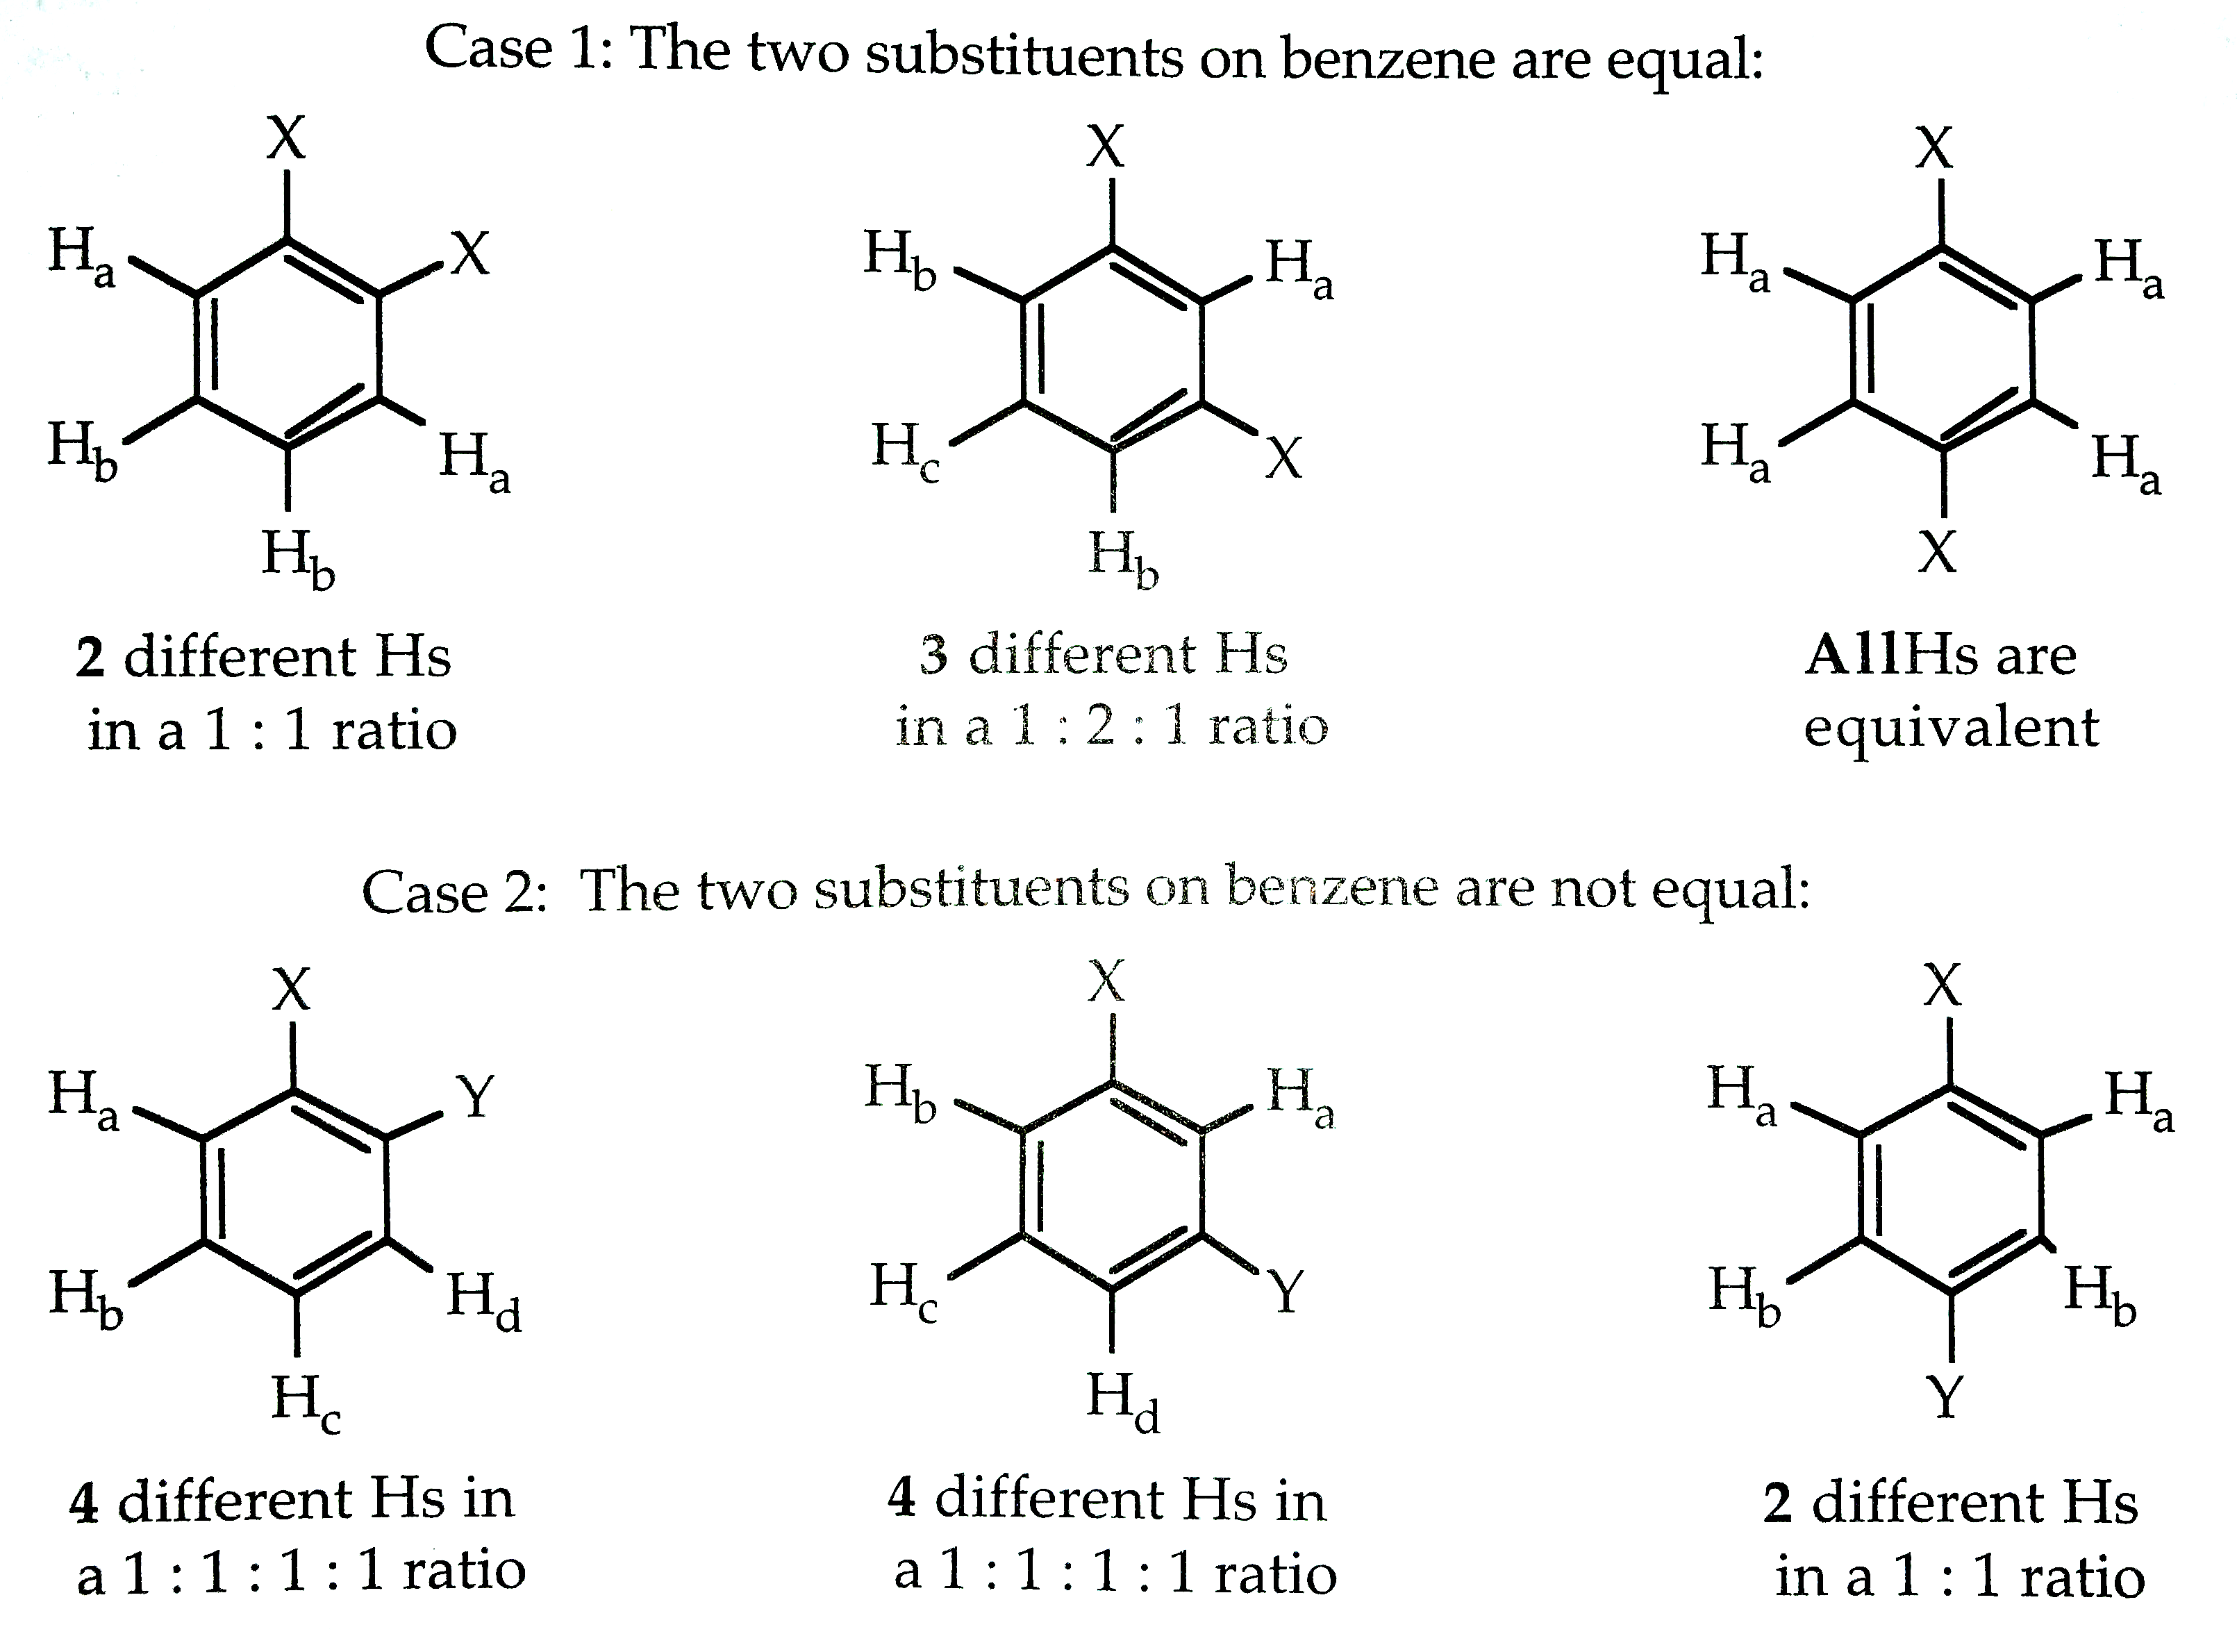
\includegraphics[width=0.7\textwidth]{benzene_nmr.png} \label{benzene_nmr}
\caption{Discussing the expected \ce{{}^1H} NMR peaks for different benzene isomers.}
\end{figure}
\indent \textbf{Deuterated Solvents for \ce{{}^1H} NMR:} Because the solvent in \ce{{}^1H} NMR is in substantially higher concentration than the solute, it is imperative that the solvent not have any hydrogens. If the solvent has \ce{{}^1H} nuclei, then it would produce the largest signal in the spectrum. To avoid this problem, solvents are chosen that have deuterium \ce{{}^2H} instead. However, one potential problem with this occurs when protic compounds are dissolved into deuterated protic solvents, such as \ce{D_2O}. Protic hydrogens can undergo exchange with the protons of the solvent, if the solvent is also protic. Although the dissociation constant may be small for compounds such as alcohols, over enough time all of the hydrogens can be released and then are able to reform their bonds. If \ce{D_2O} is present in the solution, then deuterium will gradually replace protic hydrogens capalbe of undergoing exchange. This causes the signal for the protic hydrogen to disappear gradually. \\
\indent \large\textbf{Mass Spectrometry:} \normalsize In mass spectrometry, first the molecule is first converted into a cation following the addition of some input energy. The cation is then accelerated through an electric field after which it is deflected along the circular path by a perpendicular magnetic field. The radius of the circular path correlates to the particle's mass-to-charge ratio. In general, when ionizing a hydrocarbon, a bonding electron is lost from a \ce{C-H} bond. Because cations and free radicals are unstable, the species rearranges and fragments, sheering off pieces of the molecule. \\
\indent The base peak is the most intense peak, and the parent peak is the peak of the original molecule without any fragmentation. In mass spectroscopy, the material being analyzed should be at low pressure (so that the reactive free radical and cationic particles do not collide and undergo reactions), and also in the gas phase (so that the particles travel independently of one another in the apparatus). \\
\indent Mass spectrometry is particularly useful in detecting chlorine and brome, because for both of these there are two predominant isotopes in a high concentration. This ratio is easily recognized when viewing the results from mass spectrometry. Elemental bromine is about 50\% \ce{{}^{79}Br} and 50\% \ce{{}^{81}Br}, so mass spectrometer results for compounds with bromin show two peaks of roughly equal size separated by 2 atomic units (amu). This is a telltale feature of a compound that contains a single bromine atom. Elemental chlorine is about 75\% \ce{{}^{35}Cl} and 25\% \ce{{}^{37}Cl}, so mass spectrometer results for compounds with a single chlorine show two peaks with a 3:1 size ratio separated by 2 atomic mass units. No other elements common in organic molecules have isotopes separated by two amu with such large population percentages. 

\subsection{Lab Techniques}
Lab techniques can be broken down into three categories: separation, purification, and identification.\\
\indent \large\textbf{Separation} \normalsize of molecules requires that at least one of the molecules be in motion. We shall use the word \textit{flow} to describe the motion of bulk material. The ability to flow depends on the state of matter. When two materials are in different phases, they can flow in different directions and therefore can be separated. A common sense view of separation techniques dictates that if you have a mixture of two or more components, you must convert the system into a state where the components are in different phases.\\
\indent \textbf{Distillation} removes a liquid from either another liquid or from solute by exploiting their boiling point differences. Upon heating, the most volatile component converts to a gas more readily than the less volatile components. This vapor distillation purification cycle is repeated multiple times until the desired purity is achieved. This is what is referred to as \textit{fractional distillation}. If it is only done once, it is called \textit{simple distillation}. Simple distillation is employed with liquids that have a large difference in boiling points, and also to remove a solvent from a solute. Simple distillation is faster than fractional distillation and it generates a higher yield, while fractional distillation leads to greater distillate purity. A typical distillation apparatus is shown in \textbf{Fig. \ref{distillation}}.\\
\indent \textbf{Chromatography} is the separation of two or more components in a mixture by exploiting their differences in (1) solubility in a migrating solvent and (2) their affinity for a polymer. The mobile phase is one of several possible solvents, ranging from nonpolar to polar/protic, or in some instances a mixture of two solvents. The stationary phase is one of two materials: alumina or silica gel. Both of these polymers are polar, so in the absence of any other information, we know that polar materials have a higher affinity for the stationary phase than nonpolar materials. As a consequence, polar species have slower migration rates than nonpolar species in chromatography. \\
\indent \textbf{Thin Layer Chromatography (TLC)} is carried out on a small scale to identify the number of components or type of components in a mixture. It involves spotting small aliquots of sample near the bottom of a vertical, rectangular plate with either silica gel or alumina on its surface in a line parallel to the base of the plate. This plate is then placed into a container that can be fitted with a lid and solvent is added to the container until it is just below the level of the spots. Due to capillary action, the solvent slowly migrates up the plate, interacting with each of the spots as it travels. In order to prevent eh solvent from evaporating, a lid is employed to maintain a closed system. Once the plate is developed, once can ascertain where the spots ended, and thus know how many components where in the mixture and whether the components were nonpolar, semi-polar, or highly polar. A typical TLC set up is shown in \textbf{Fig. \ref{distillation}}. \\
\begin{figure}[!ht]
\centering
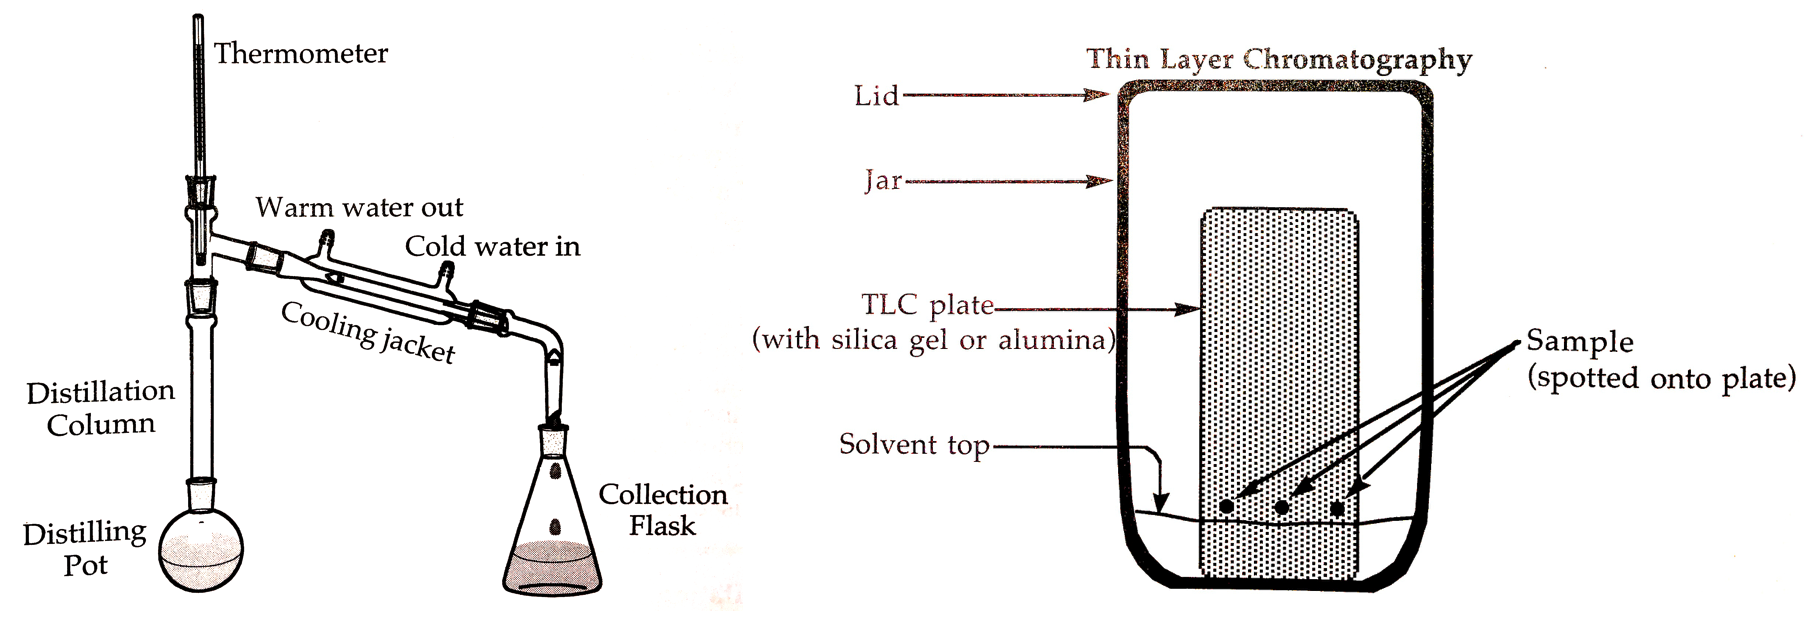
\includegraphics[width=0.7\textwidth]{distillation.png} \label{distillation}
\caption{\textit{Left} A typical distillation apparatus/setup. \textit{Right} A typical thin layer chromatography setup.}
\end{figure}
\indent In TLC, we often measure an $R_f$ value for the compounds, which we can think of as a `ratio of the fronts,' where the distance a spot travels is compared to the distance that the solvent travels. The component with the greatest $R_f$ value is the component that has the least affinity for the stationary phase (adsorbent) and is the most soluble in that solvent. The range for $R_f$ values is $0\leq R_f < 1$, because there is a chance the spot does not travel at all or that it travels almost at the solvent front. Because a solute dissolves best into a solvent of `like' nature, the higher the value of $R_f$ value, the more that the solute is like that solvent. Based on $R_f$ values, you should be able to make predictions as to the best solvent for column chromatography. The best separation occurs when the $R_f$ values have the greatest ratio. The basic idea of all forms of chromatography is \textit{separation by relative affinity}. \\
\indent \textbf{Column chromatography} is applied to separate bulk quantities of product. It operates on the same principles as TLC: the solubility of a compound in the solvent as it flows down the column versus the affinity of the compound for the absorbent in the column. If the compound migrates quickly down the column, we can conclude that it must experience a minimum attraction to the silica gel or alumina (stationary phase) in the column. The sample and solvent flow down the column; faster migrating compounds reach the bottom of the column first, so they have shorter elution times. A large $R_f$ value corresponds to a low elution time, given that the compound has a fast migration rate in each case.\\
\indent \textit{Chiral columns} have become popular in recent years, because they are capable of selecting for one enantiomer over another. The most common designer polymers on the MCAT to date are the adsorbents used in ion exchange chromatography. Three with which you should be familiar are \textbf{sulfonated-polystyrene}, \textbf{carboxymethyl-cellulose (CM-cellulose)}, and \textbf{diethylaminoethoxy-cellulose (DEAE-cellulose)}. The first two carry negative charges at neutral pH, while DEAE-cellulose carries a positive charge at neutral pH. These allow us to isolate the oppositely charged proteins based on electrostatic interactions.\\
\indent \textbf{Gas chromatography (GC)} works by first vaporizing a sample (mixture of components) into the gas phase and then forcing that organic vapor through a packed column using elevated pressure from a cylinder of an inert gas. The machine measure retention time on the column by recording collisions as gas molecules leave the end of the long, coiled column and strike the detector. The collisions are converted to peaks, which can be integrated to determine their relative abundance. The compounds in the sample must be highly volatile at $200^{\circ}$C and inert with regards to silica gel or was for GC analysis to work. \textbf{Fig. \ref{gc}} shows the design for a standard gas chromatography machine. Given that the compounds vaporize instantaneously upon addition to a GC machine, the boiling point does not affect the elution time. However, because many columns are often slightly polar, affinity for polar species is greater than affinity for nonpolar species. A second factor that dictates the migration rate is mass\textemdash heavier gases move slower and have longer elution times. heavier gases and polar gases typically have high boiling points, so although boiling point has little to do with elution time, the factors that raise boiling point also increase the elution time in a GC.\\
\indent \textbf{Extraction} works based on solubility and it's typically employed to take advantage of drastic difference in the solubilities of components in two different (immiscible) solvents. First, we need to define \textbf{partitioning} A compound has a different solubility in every solvent. The ratio of its maximum solubility in one solvent compared to its maximum solubility in another solvent is known as the \textit{partition coefficient}. In cases where the compound can go into either solvent, it will select between the solvents in a ratio equal to the partition coefficient. When the solvent system involves two immiscible liquids, then the solute must split between the two solvents. This means that the components of a mixture can be separated if they have different partition coefficients. By decanting one solution from the other, the components are then separated from one another in their solute form according to their relative solubilities in the two different solvents.\\
\indent When one of the two immiscible solvents is water, the solubility properties of the solutes can vary with the water pH. \textbf{Acid-base extraction} separates compounds by their pK\textsubscript{a} values. Here is an example problem:
\begin{center}
\begin{minipage}{30em}
\textcolor{blue}{To separate benzoic acid (\ce{C_6H_5CO_2H}) from toluene (\ce{C_6H_5CH_3}), it would be best to use a mixture of an:
\begin{enumerate}[label=\Alph*]
	\item alcohol and water at pH=11.
	\item alcohol and water at pH=3.
	\item ether and water at pH=11.
	\item ether and water at pH=3.
\end{enumerate}}
\end{minipage}
\end{center}
\noindent To carry out an extraction, the two solvents cannot be miscible in one another. Alcohols are typically miscible in water, so choices A and B are eliminated. Benzoic acid can be deprotonated in basic solution, where it becomes its anionic conjugate base (benzoate), which is readily soluble in water. Toluene is nonpolar and thus dissolves into the organic ether rather than water, so the best answer is choice \textbf{C}.\\
\indent On the MCAT, perhaps the most difficult task when it comes to extraction will be analyzing a flow chart. \textbf{Fig. \ref{extraction}} shows a typical four-compound flow chart. It is a good general rule that a weak base should be added before a strong base, so as to isolate the stronger acid. If you were to add the sodium hydroxide first, it would extract both the phenoxide and the carboxylate into the aqueous layer. Also, because extraction involves both acidic water and basic water, there is the potential for hydrolysis. As such, extraction cannot be used to isolate water-sensitive compounds such as acid anhydrides, acid halides, and esters.\\
\begin{figure}[!ht]
\centering
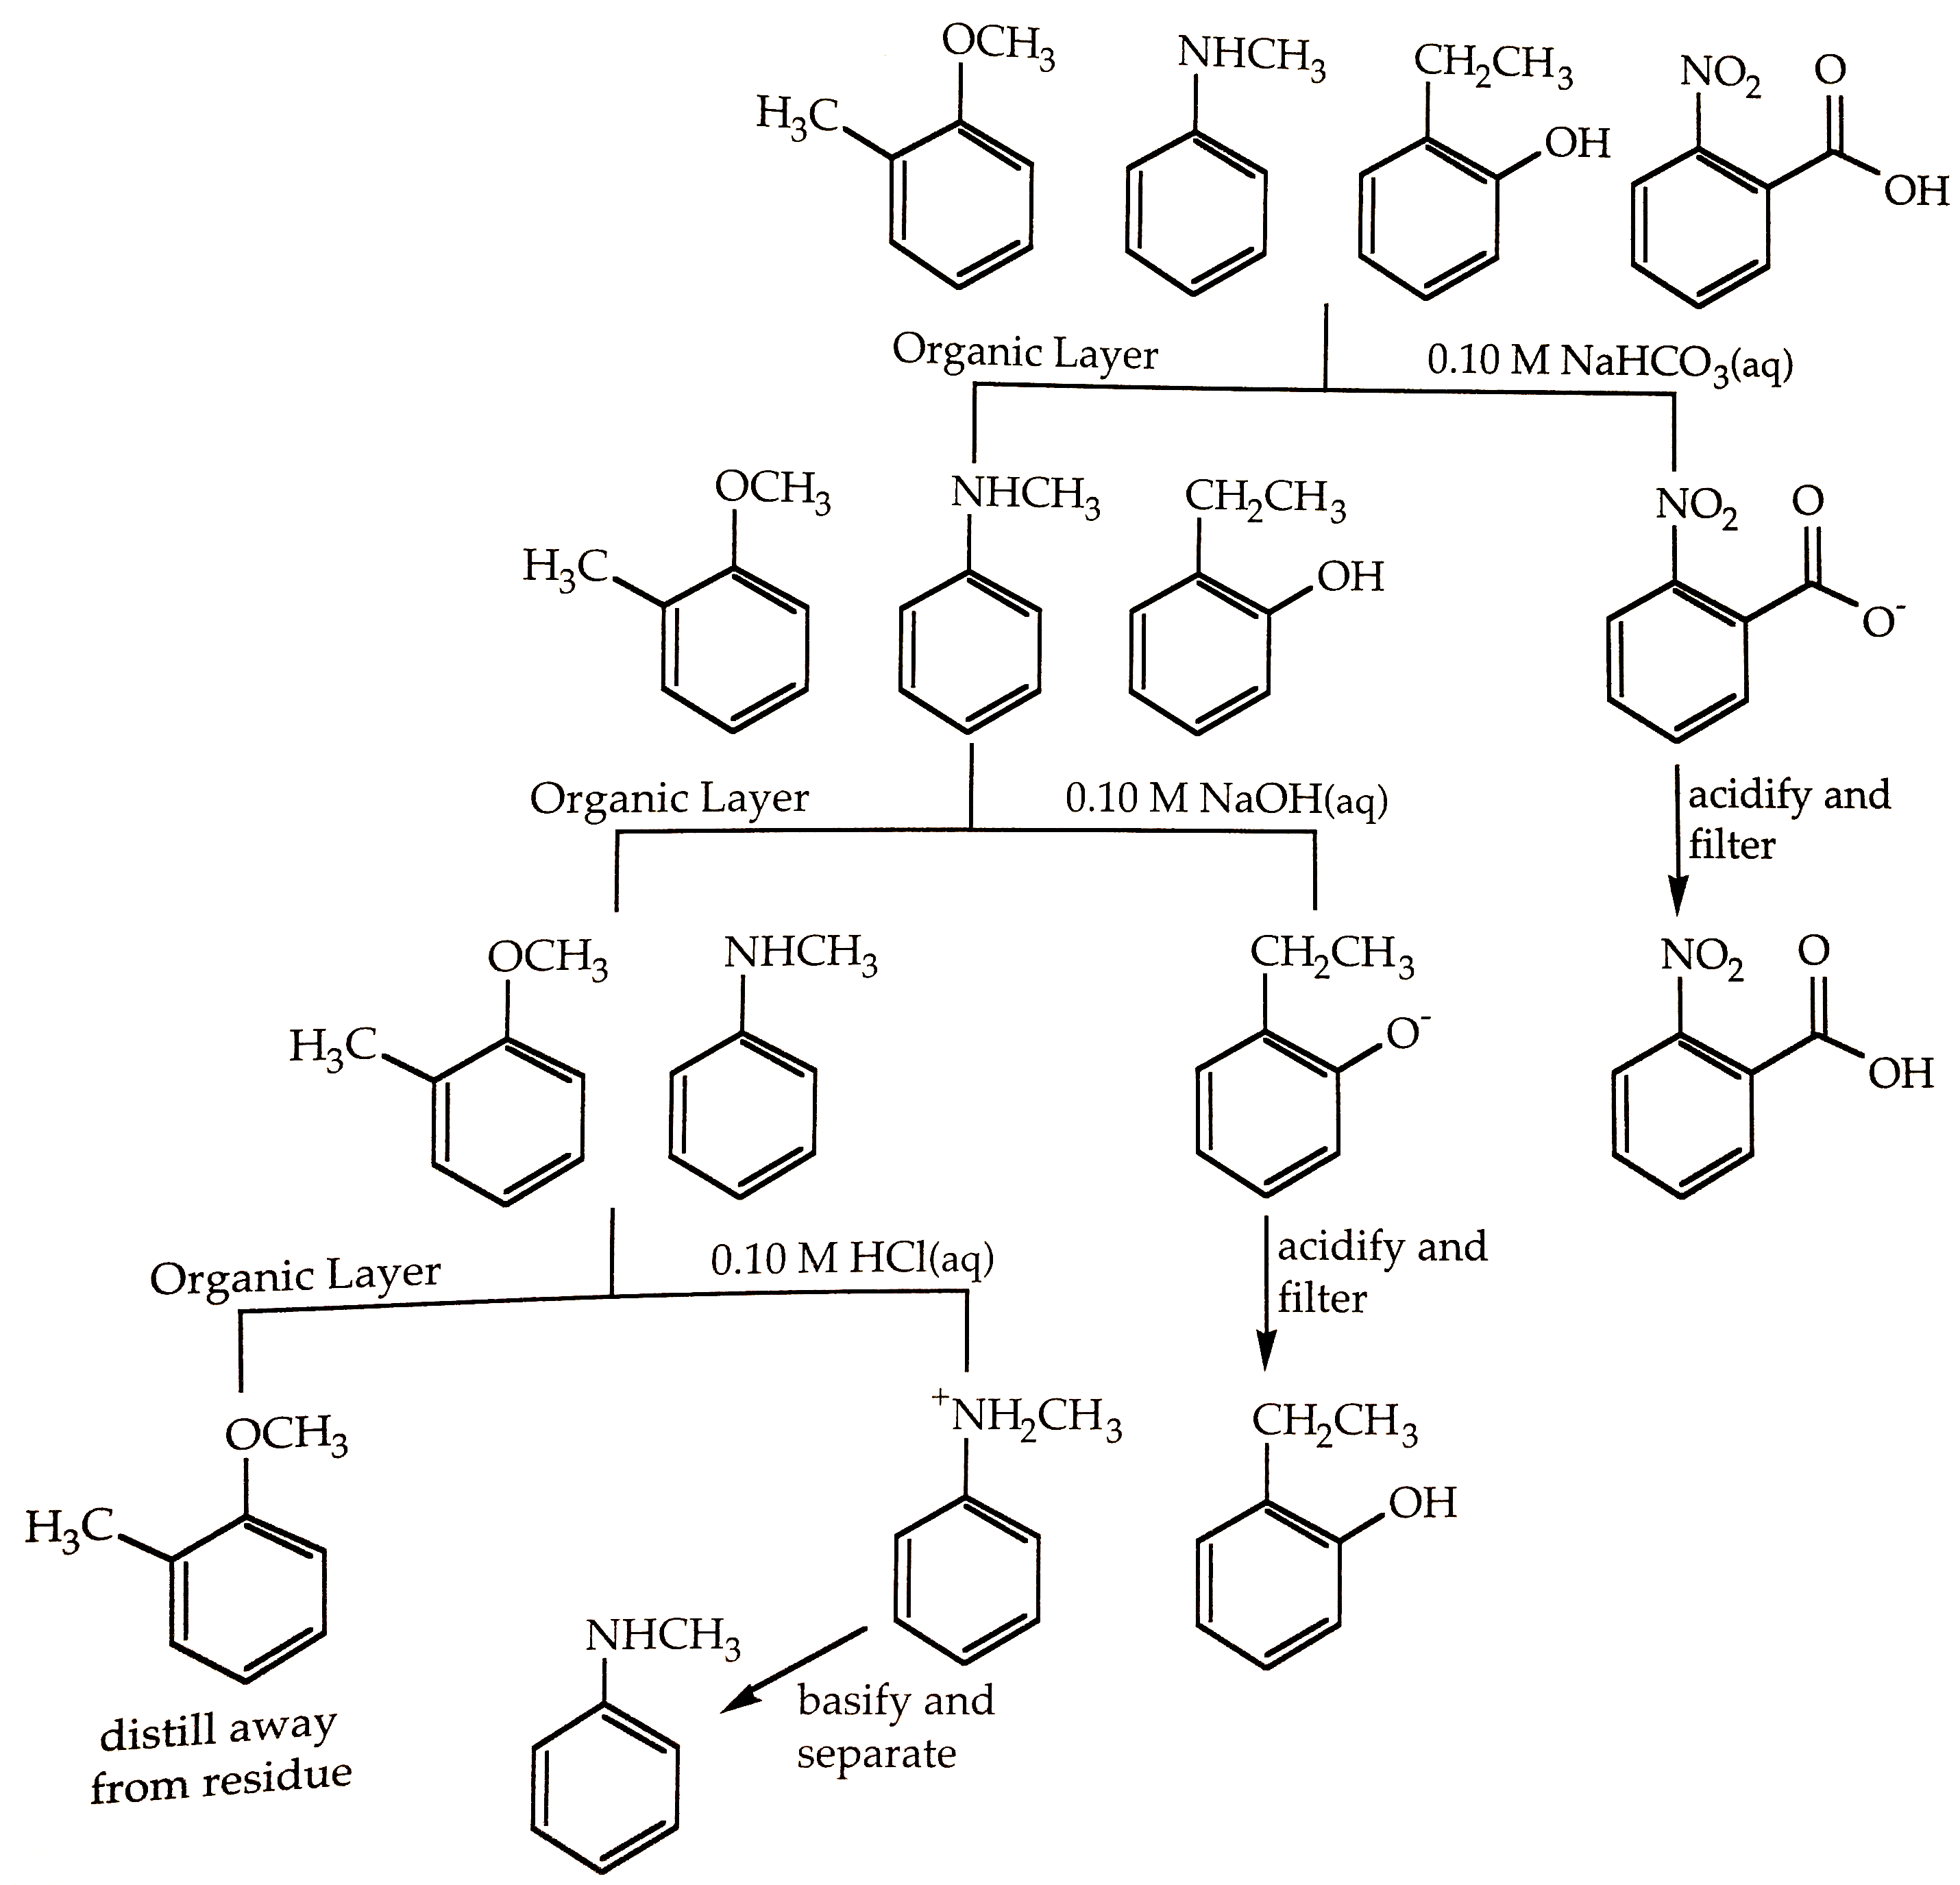
\includegraphics[width=0.7\textwidth]{extraction.png} \label{extraction}
\caption{An example extraction flow chart.}
\end{figure}
\indent \large\textbf{Purification:} \normalsize Many of the separation techniques we have discussed so far can also be used as purification techniques. For example, column chromatography is useful for purification, because the bands separate nicely from one another. A solid product may be separated from solid impurities through selective precipitation, which is referred to as \textbf{recrystallization}. Recrystallization involves dissolving the solid into hot solvent, hot filtering out the insoluble solid impurities, and then slowly cooling the solution to precipitate the purified crystals. Upon cooling the solution, the product precipitates out of solution in a crystalline form free of the impurities from before. The crystals are filtered at low temperature, to prevent any of the material from dissolving back into solution, to avoid any reduction in the yield.\\
\indent Solvent choice is essential in recrystallization. In order to maximize the amount of crystal collected, the desired material should be insoluble (or minimally soluble) in the solvent at lower temperatures. Sometimes the solvent can be a homogeneous mixture of two solvents to meet desired solubility properties. \\
\indent In some instances, the purification can be enhanced by adding a material to preferentially bind some or all fo the impurities. One such case occurs when you have colored impurities and a colorless target crystal. By adding activated charcoal (charcoal that is free of impurities), the colored species will be preferentially bound by the surface of the charcoal and can thus be filtered out. Charcoal binds all organic materials, but because of its $\pi$-network and the presence of conjugated $\pi$-networks in colored species, charcoal has a higher affinity for colored organic molecules than colorless organic molecules.\\
\indent \textbf{Filtration} is employed to remove solids from liquids. A fine microscopic net is used to separate the solid from the liquid by allowing the liquid to flow through while hindering the flow of solids, which are larger than the pore size of the filter. Filtering typically depends on gravity to force the liquid to flow through the filter, although it can be expedited by a vacuum pressure difference.\\
\indent The final step of crystallization is cold filtering (cold to prevent the loss of product to dissolving) and washing the precipitate with a solvent that does not dissolve the target compound, but dissolves the impurities. It is optimal to use a solvent with a low boiling point, so it can readily evaporate away from the solid. Here are a couple practice problems regarding purification:
\begin{center}
\begin{minipage}{30em}
\textcolor{blue}{If a solid is too soluble in water at room temperature, it would be best to add which of the following solvents?
\begin{enumerate}[label=\Alph*]
	\item Hexane
	\item Ethanol
	\item Diethyl ether
	\item Tetrahydrofuran
\end{enumerate}}
\end{minipage}
\end{center}
\noindent They key to this question is that the solvent you mix with water must reduce the overall polarity and hydrogen bonding capacity of the solvent mixture \textit{and} be soluble in water. All of the choices are less polar and less protic than water, but of the choices, only ethanol is soluble in water. Choice \textbf{B} is therefore the best answer.
\begin{center}
\begin{minipage}{30em}
\textcolor{blue}{Which of the following mixtures can be separated using gravity filtration?
\begin{enumerate}[label=\Alph*]
	\item Ethanol from diethyl ether.
	\item Sodium chloride from water.
	\item Butane from dichloromethane.
	\item Oxalic acid from hexane.
\end{enumerate}}
\end{minipage}
\end{center}
\noindent In choice A, both compounds are liquids, so filtering is pointless. In choice B, the salt is completely soluble in water, so the salt is actually in solute form. It must be a solid, not solute, to be filtered, so choice B is eliminated. Butane is a liquid as is dichloromethane, eliminating choice C, leaving choice \textbf{D} as the correct answer. Hexane is a liquid and all carboxylic acid, besides formic acid and acetic acid, are solids at room temperature. Acids to not readily dissolve into hydrocarbon solvents, so oxalic acid exists as a solid and not as a solute in hexane.\\
\indent \large\textbf{Identification Techniques:} \normalsize You can (somewhat) identify/verify a compound or ascertain its purity from its melting point. A rapid change from a solid into a liquid is indicative of a pure compound. Here is an example problem:
\begin{center}
\begin{minipage}{30em}
\textcolor{blue}{If a student suspects that the compound they have is L-tyrosine, what should they add to the sample for a mixed melting point?
\begin{enumerate}[label=\Alph*]
	\item L-Tyrosine
	\item D-Tyrosine
	\item Xylose
	\item Glycine
\end{enumerate}}
\end{minipage}
\end{center}
\noindent To support the notion that an unknown compound is L-tyrosine using a mixed melting point study requires mixing the unknown with a pure sample of L-tyrosine. If the unknown compound is in fact L-tyrosine, then the mixture is in fact pure L-tyrone. This would result in a sharp melting point at the characteristic melting point of L-tyrosine. If the unknown compound were not L-tyrosine, the melting point range would be broad and would fall outside of the characteristic melting point of L-tyrosine.\\
\indent \textbf{Chemical tests} involve reactions that are selective for very few functional groups. The ideal chemical test is positive for only one functional group, but this is rare. Most chemical tests have multiple functional groups that give positive results. For a chemical test to be effective, a few things must be true:
\begin{enumerate}
	\item The reagent must react with very few functional groups.
	\item The chemical testing reagent must undergo some visible change, such as a color change or phase change, so it can be detected.
	\item The testing reagent must be the limiting reagent, so that any excess of the testing reagent will not interfere with the reading. 
\end{enumerate}
\indent \textbf{Derivative} are products formed from the reaction of a given reagent with an unknown compound, Derivatives are made to be used as a diagnostic for an unknown. The additional physical measurements associated with the newly formed derivative can be used to identify both the derivative and indirectly the unknown. They are used to support and confirm an identity for an unknown. Common derivatives include 2,4-dinitrophenylhydrazones for ketones or aldehydes, benzylesters for alcohols, and osazones for sugars. The ideal derivative is a solid that can easily be identified by its melting point.

\subsection{Lipids}
Lipids are natural molecules rich in long-chain alkyl groups that share many properties with hydrocarbons, especially solubility. Lipids include fats, fat-soluble vitamins (in particular vitamins A, D, E, and K), some hormones, sterols (steroid alcohols), waxes (esters with a long-chain fatty acid combined with a long-chain alcohol), and fatty acid esters of glycerol such as monoglycerides, diglycerides, triglycerides, and phospholipids. There are insoluble in water and thus require assistance when being transported through the body. We shall define lipids as any bioorganic molecule that is not soluble in water. \\
\indent Fatty acids are carboxylic acids that have a long, aliphatic chain. Most naturally occurring fatty acids contain an even number of carbons and are unbranched. This is because the natural building block for fatty acid biosynthesis is the 2-carbon species, \textbf{acetyl CoA}\textemdash its structure is shown as a part of the synthesis pathways shown in \textbf{Fig. \ref{lipid_synthesis}}.\\
\indent \textbf{Waxes} are the esters of fatty acids, involving long-chain alcohols. The result is a highly hydrophobic ester with a high melting point. \textbf{Soaps and detergents} are amphipathic molecules, which means they contain both a hydrophobic region and a hydrophilic region. As a result, they act like surfactants when added to water. \\
\indent \textbf{Fatty Acids Derivatives} and especially straight-chain fatty acids are naturally synthesized from \textbf{acetyl-CoA} and \textbf{malonyl-CoA} via a five-step cycle that adds two carbons to the chain and then is repeated until the fatty acid backbone is complete. From there, the fatty acid has a few potential pathways, including being stored as a triglyceride or becoming part of a phospholipid. This is shown in \textbf{Fig. \ref{lipid_synthesis}}.\\
\begin{figure}[!ht]
\centering
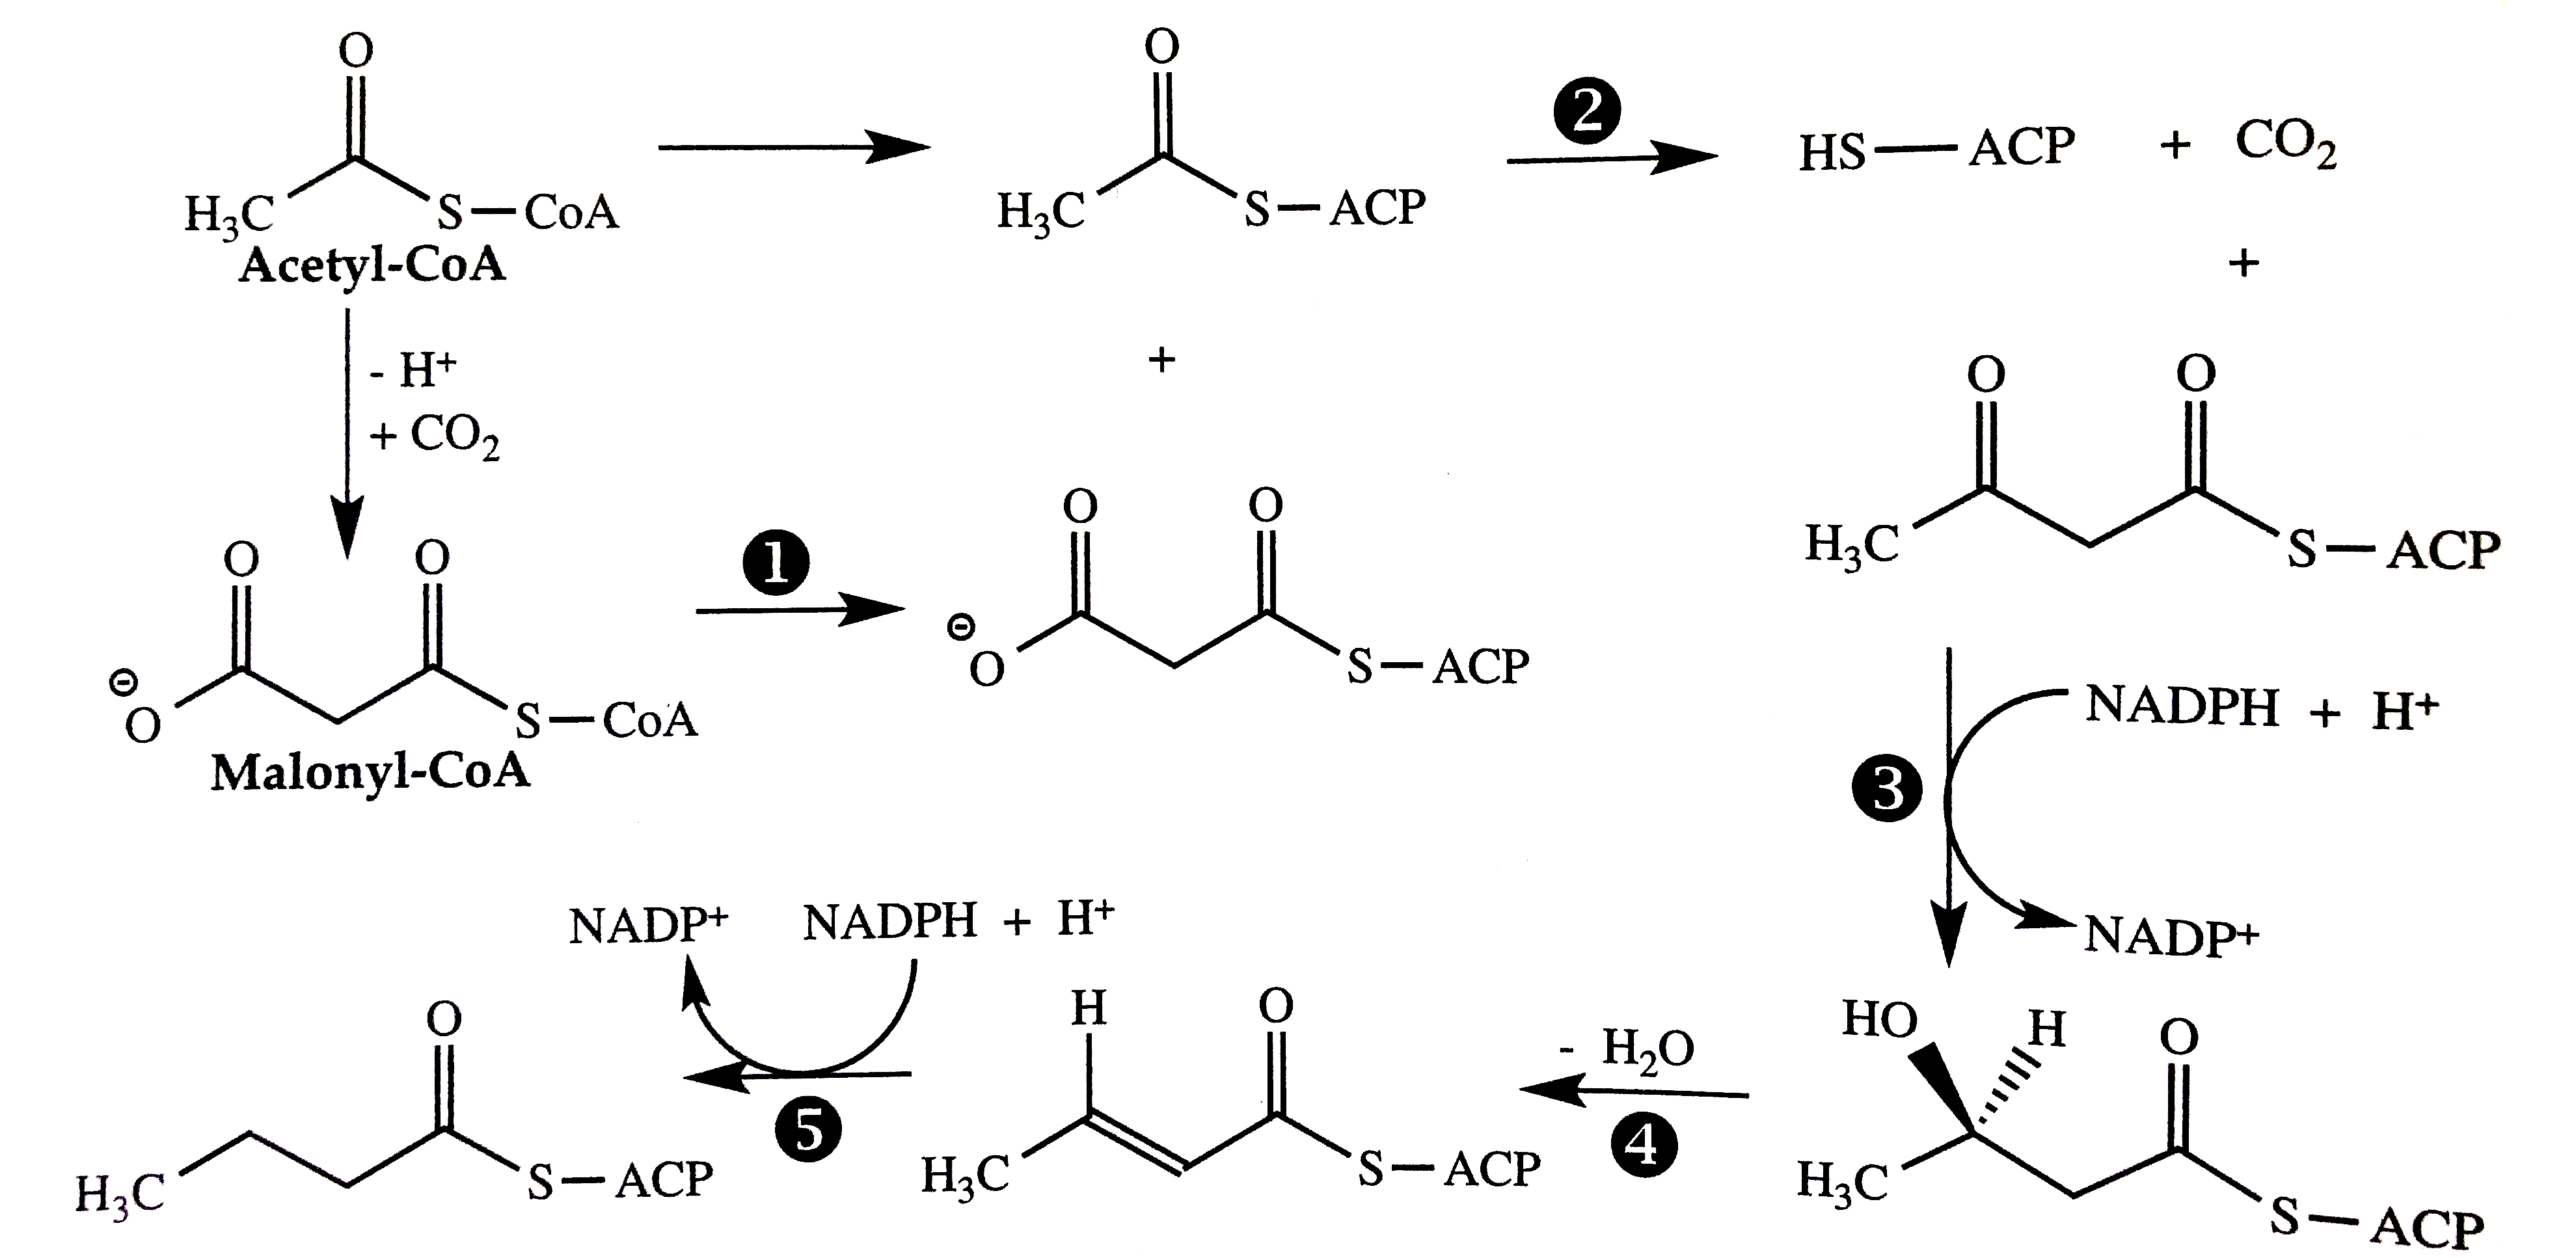
\includegraphics[width=0.7\textwidth]{lipid_synthesis.png} \label{lipid_synthesis}
\caption{Five-step cycle for the synthesis of a fatty acid backbone.}
\end{figure}
\indent From here, the fatty acid can take one of two pathways: (1) adding to glycerol-3-phosphate to become part of a cell membrane or (2) adding to a glycerol to become a triglyceride (stored fat in adipose tissue). \textbf{Fig. \ref{phosphatidate}} shows the synthesis of a phospholipid, phosphatidate. The formation of fatty acid triglycerides is similar to the formation of a phospholipid, although the final product is completely hydrophobic. \textbf{Fig. \ref{triglyceride}} shows the complete synthesis of a fatty acid triglyceride from dihydroxyacetone phosphate.\\
\begin{figure}[!ht]
\centering
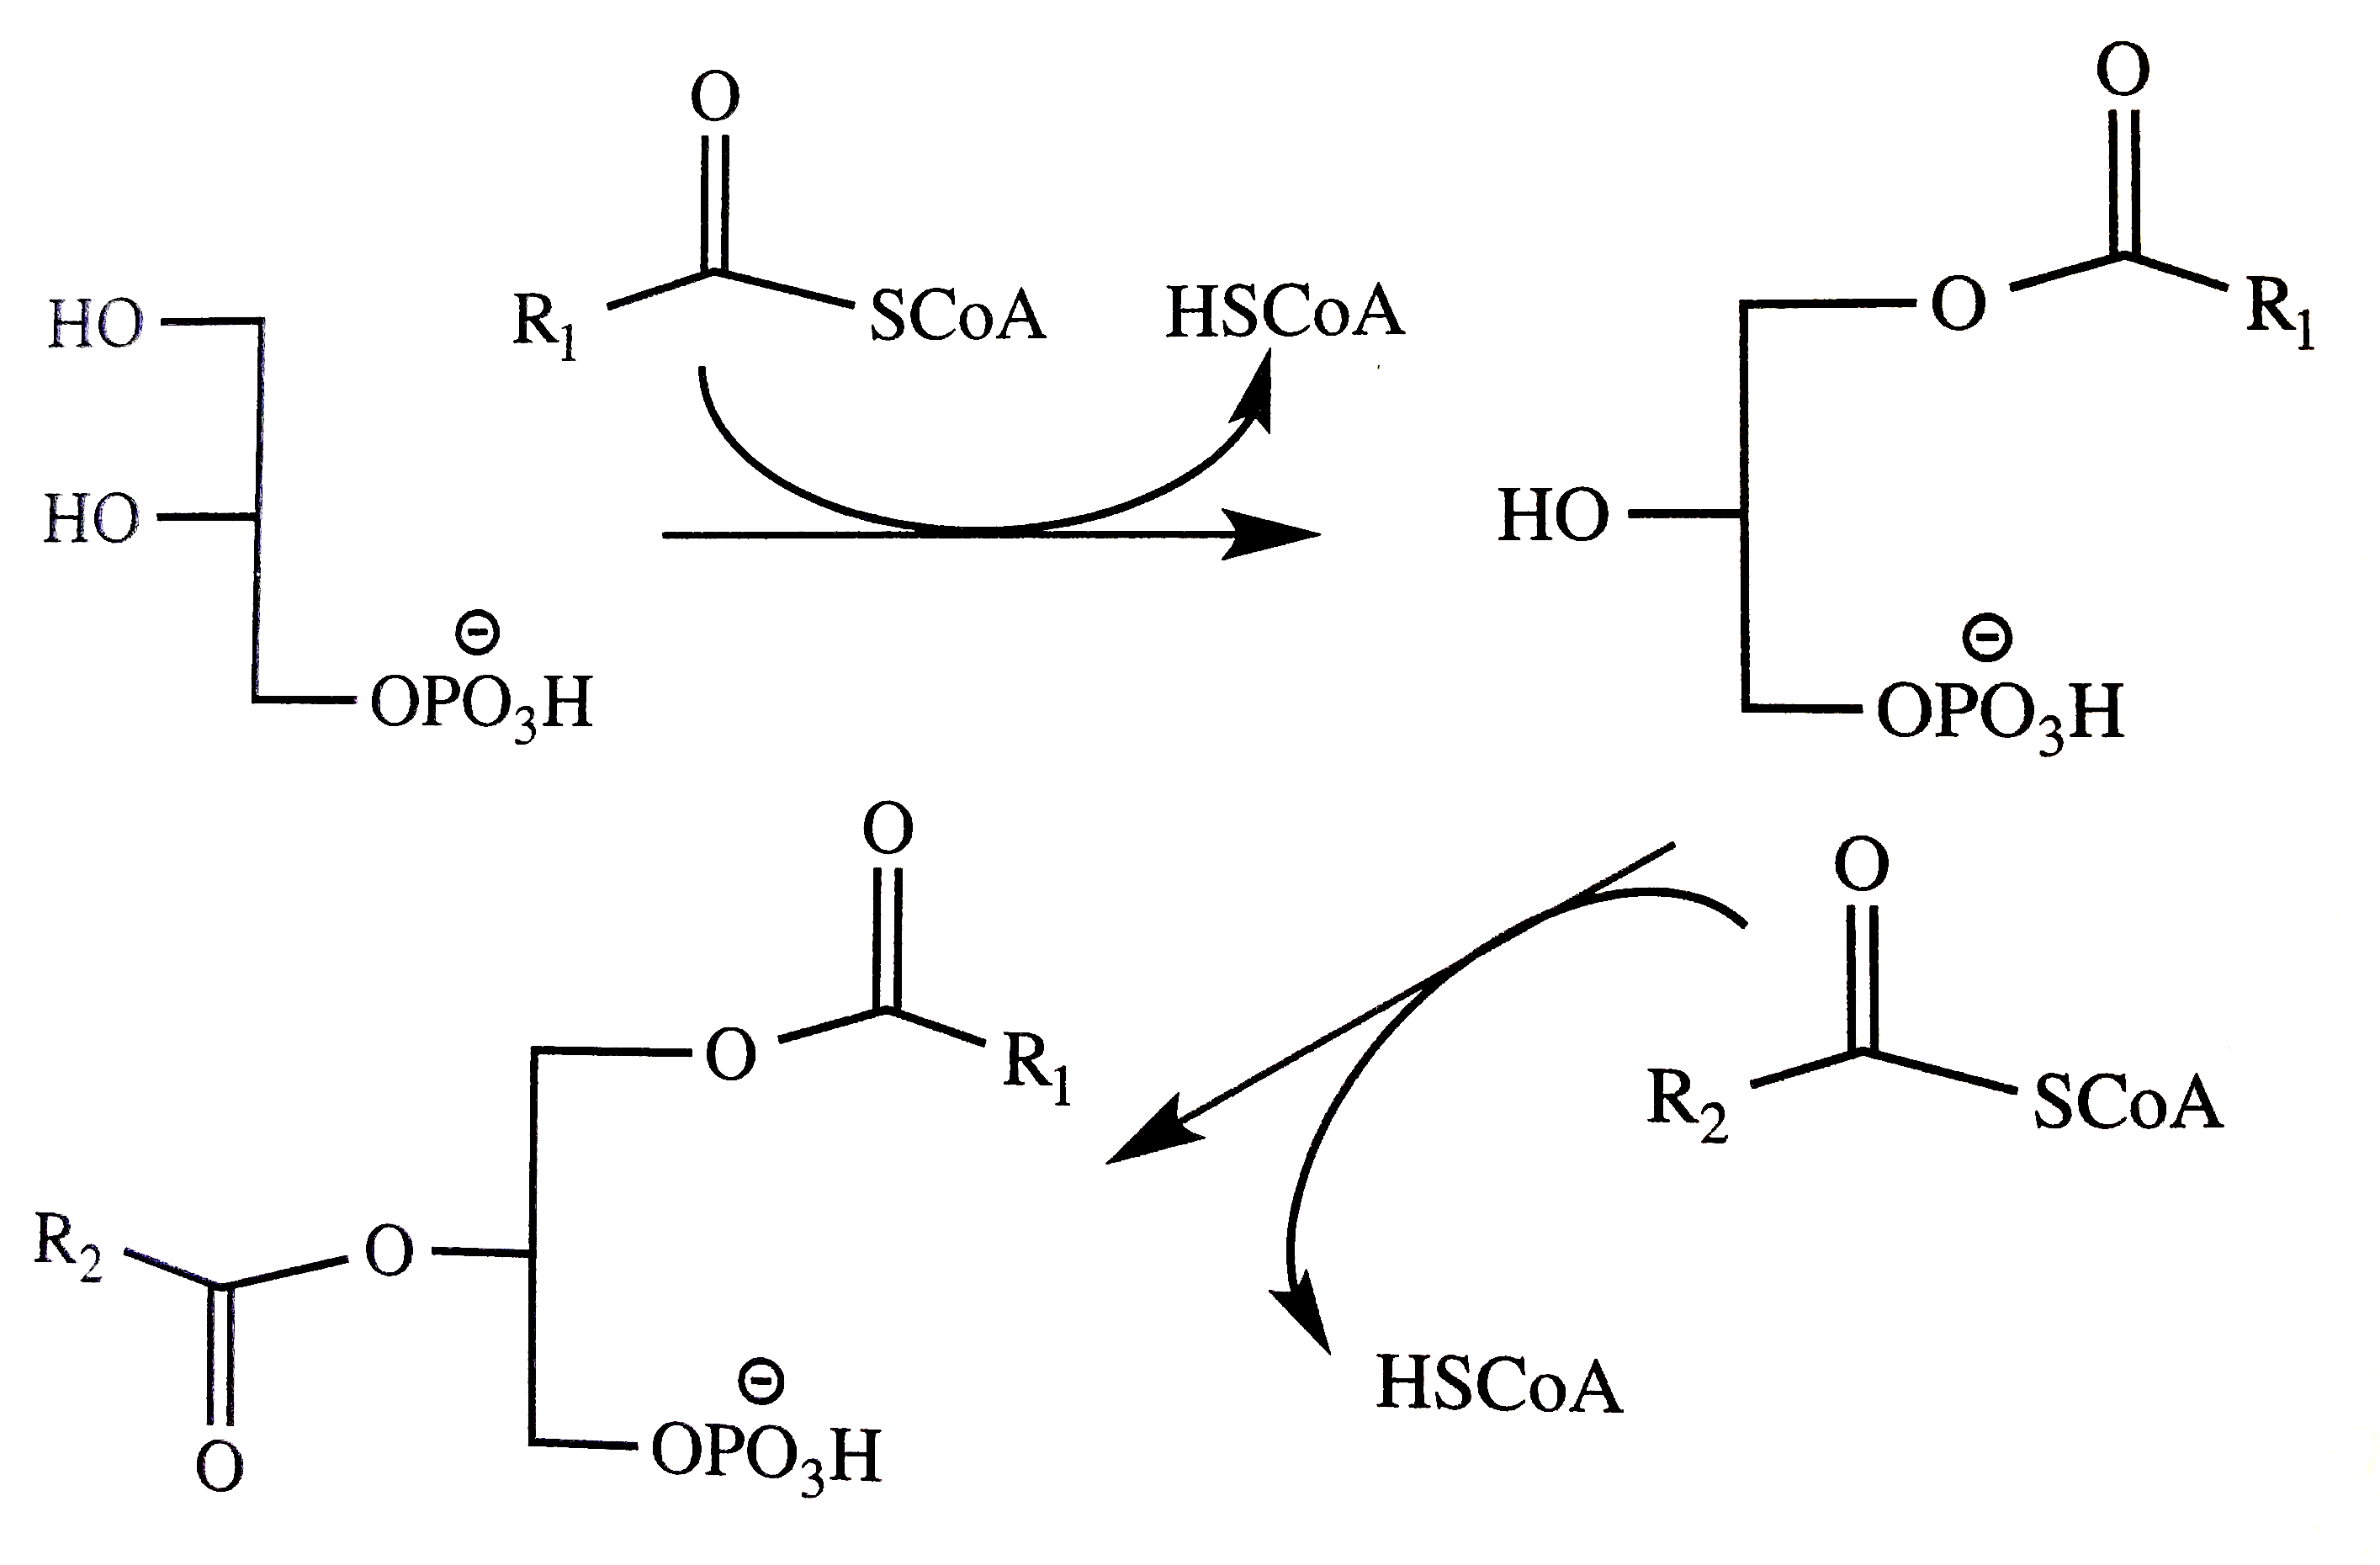
\includegraphics[width=0.7\textwidth]{phosphatidate.png} \label{phosphatidate}
\caption{Synthesis of phosphatidate, a phospholipid. In general, the first R-group (\ce{R_1}) is fully saturated while the second R-group (\ce{R_2}) is often unsaturated. The exact fatty acids depend on the cell membrane for which the phospholipid is destined.}
\end{figure}
\begin{figure}[!ht]
\centering
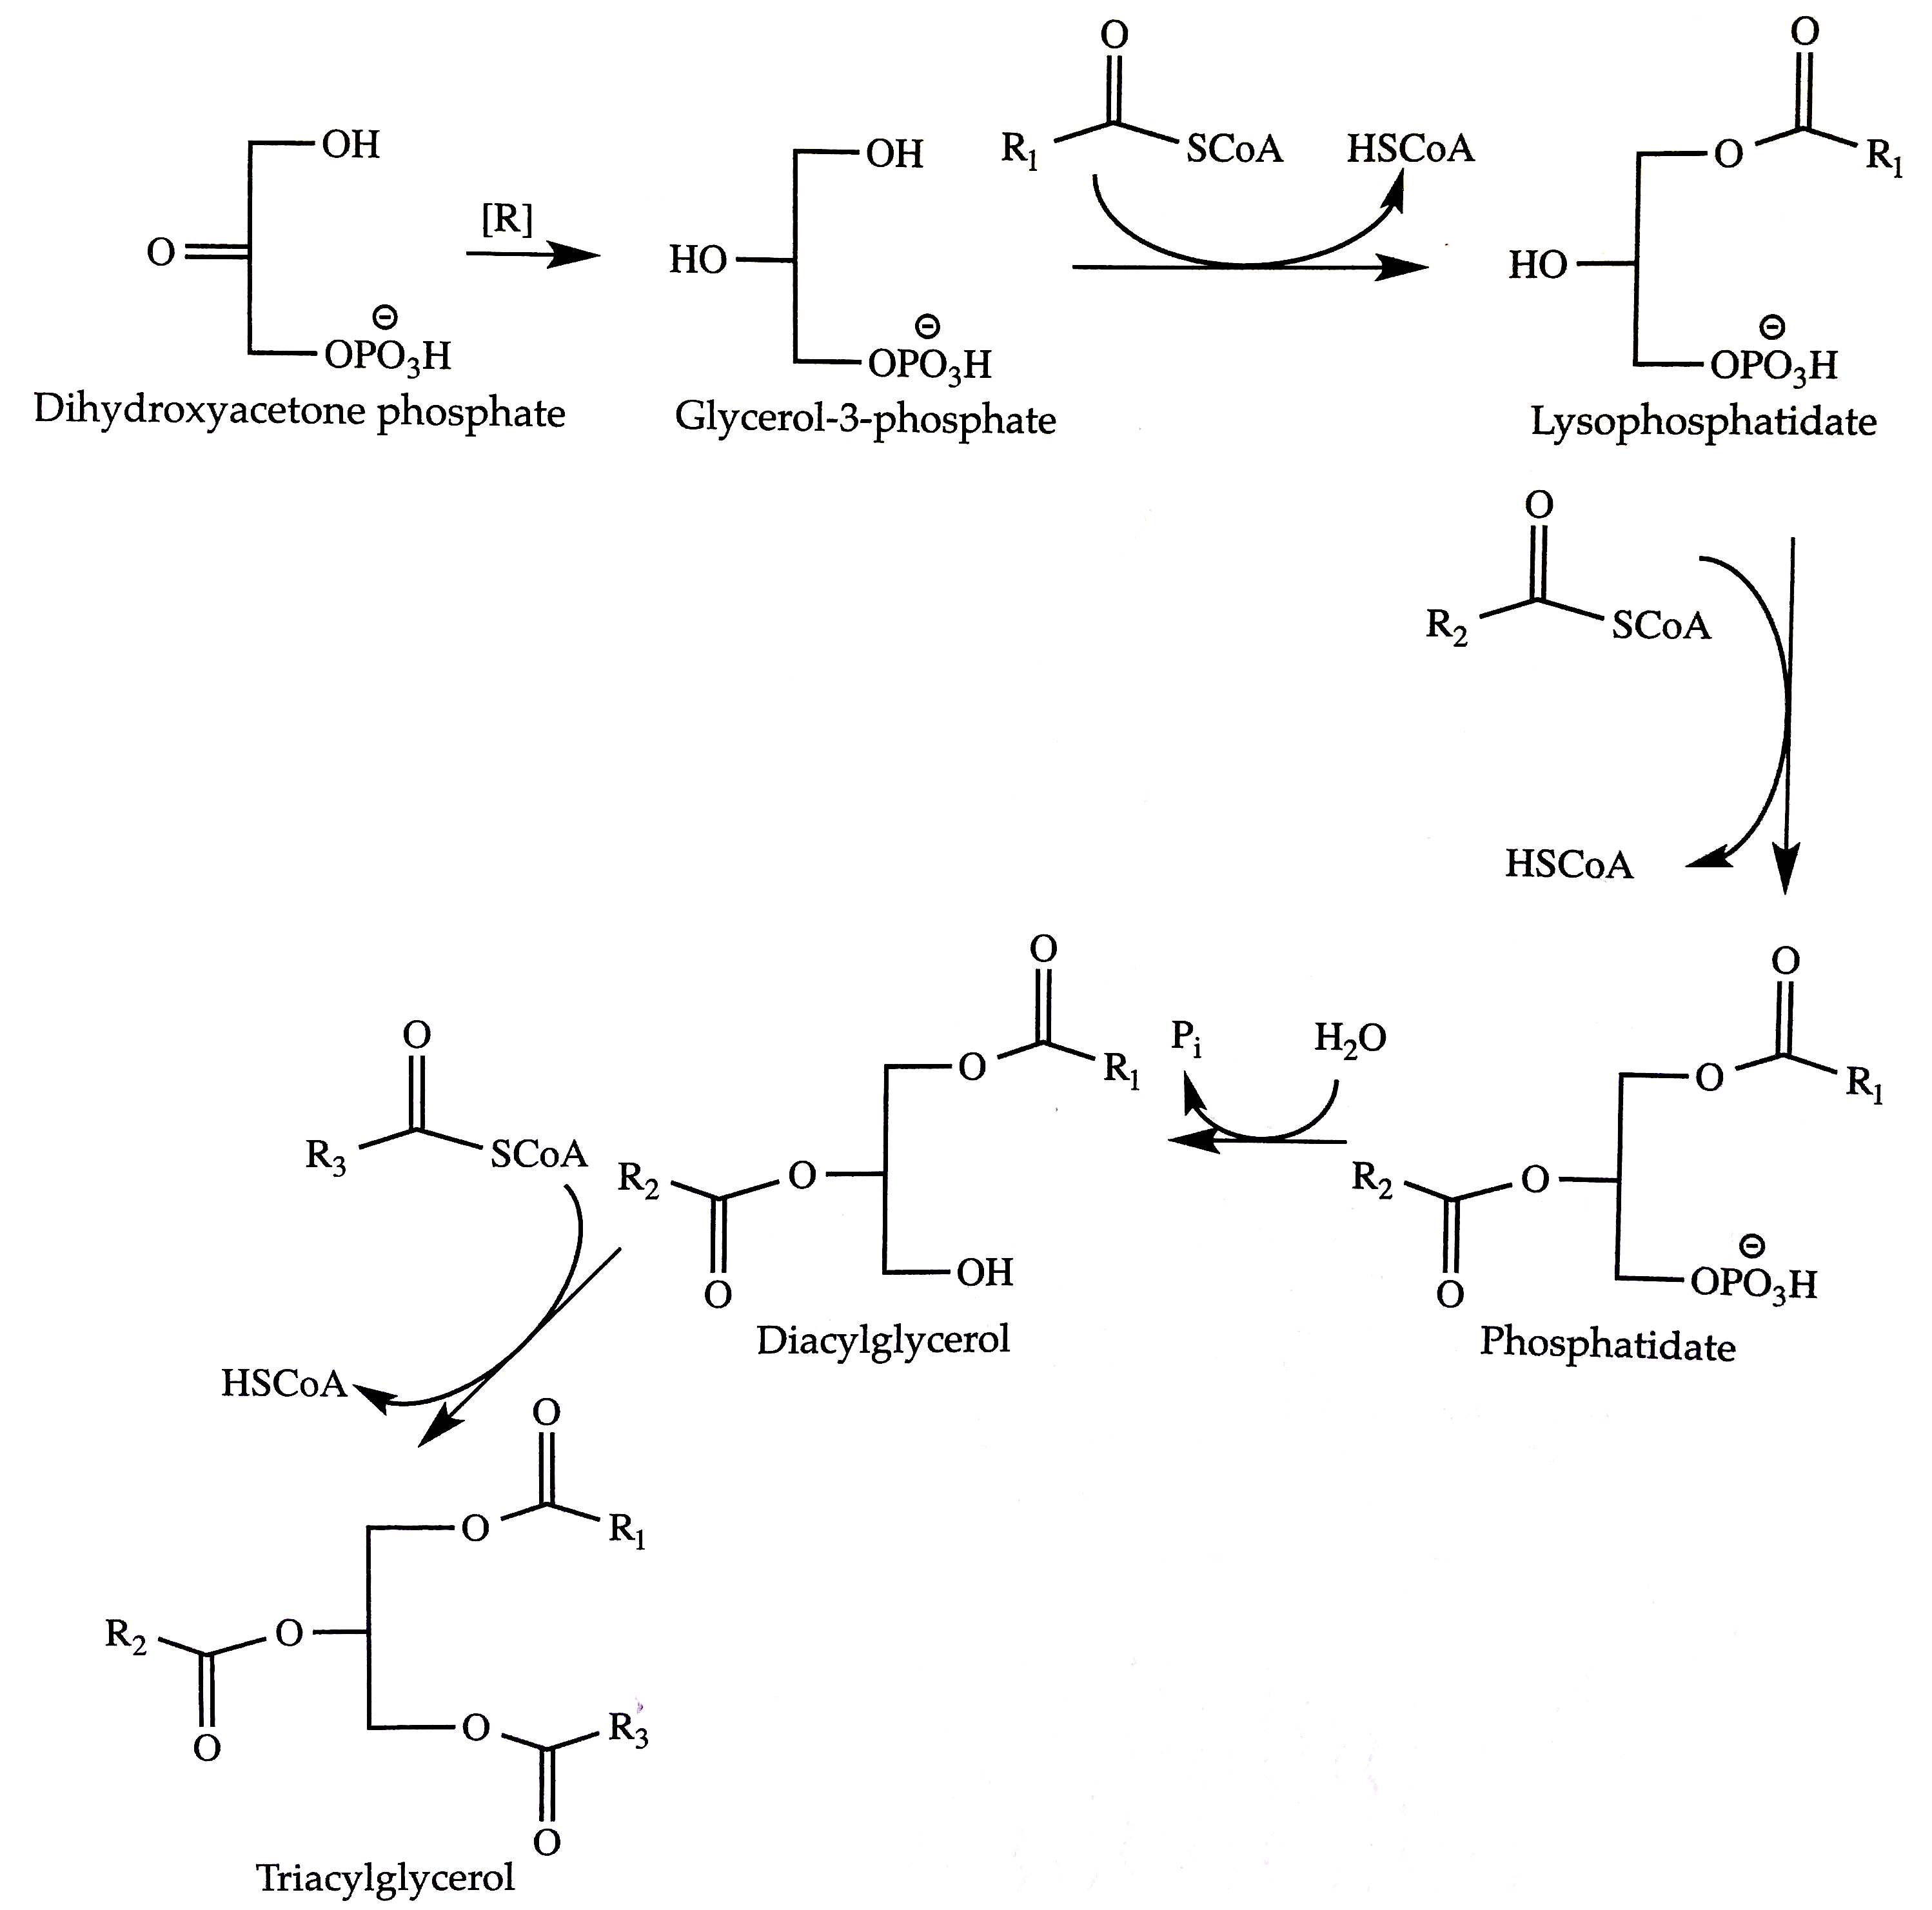
\includegraphics[width=0.7\textwidth]{triglyceride.png} \label{triglyceride}
\caption{Synthesis of the fatty acid triglyceride from dihydroxyacetone phosphate.}
\end{figure}

\subsection{Lipid Signal Molecules}
\textbf{Eicosanoids} are 20-carbon compounds derived from \textbf{arachidonate} that act as \textit{local hormones}. Eicosanoids include \textbf{prostaglandins}, \textbf{thromboanes}, and \textbf{leukotrienes}.\\
\indent Prostaglandins all share a five-membered ring from C8 through C12. They are given names PGA through PGI, where the letter refers to specific functional groups and stereochemistry. The numerical subscript refers to the number of $\pi$-bonds not in the ring. Eicosanoids are all derived from \textbf{arachindonate} through oxidation to common intermediates \ce{PGG_2} and \ce{PGH_2}. Drugs such as aspirin act on the \textit{cyclooxygenase} enzyme that is involved in the synthesis of \ce{PGG_2}. Prostaglandins are shown in \textbf{Fig. \ref{prostaglandins}}.\\
\begin{figure}[!ht]
\centering
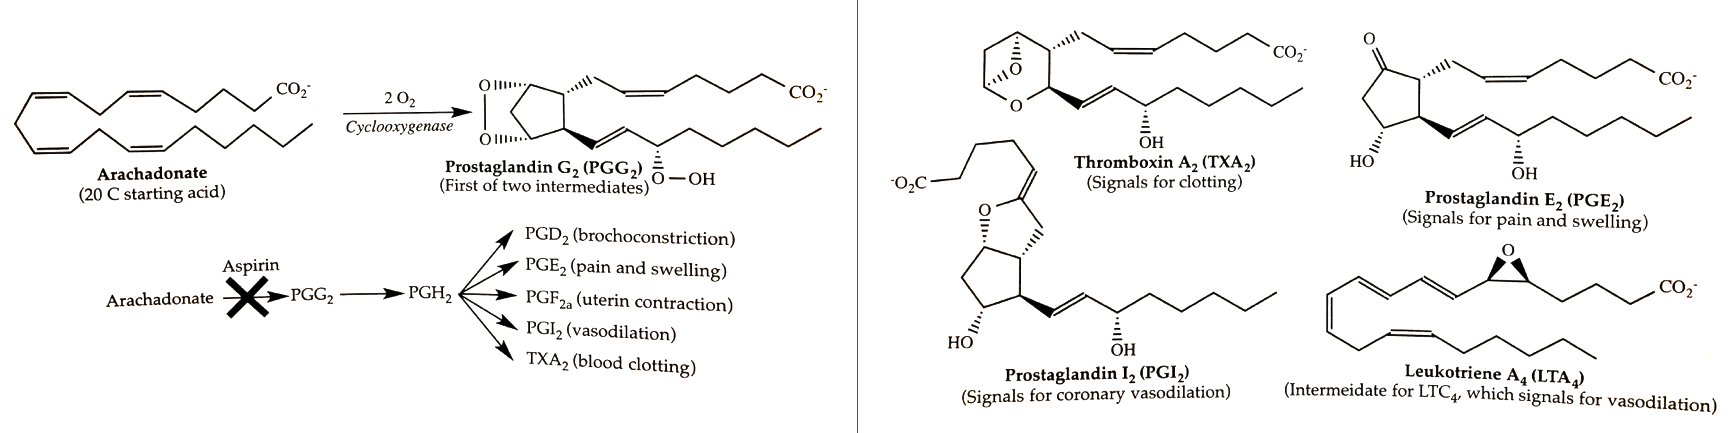
\includegraphics[width=\textwidth]{prostaglandins.png} \label{prostaglandins}
\caption{\textit{Left} Some sample eicosanoids. \textit{Right} Synthesis of eicosanoids from arachindonate.}
\end{figure}
\indent \textbf{Steroids} are a class of biological compounds that contain the \textit{androstane ring} structure (the specific four-ring structure) with various alkyl groups and functional groups. They serve many biological functions, including emulsifying fats, regulating cell membrane fluidity, and as signal molecules for many body functions. \textbf{Sterols} are a subgroup of steroids that contain hydroxyl groups, which is common in several hormones. \\
\indent \textbf{Vitamins} are nutrients that we must consume through diet. We classify vitamins according to their solubility as either \textit{water-soluble} vitamins or \textit{fat-soluble} vitamins. Water-soluble vitamins are readily passed through the body and excess quantities can be excreted as waste. Fat-soluble vitamins, on the other hand, are hard to clear from the body and therefore and reach toxic levels if consumed to excess. Four fat-soluble vitamins are Vitamin A, Vitamin D, Vitamin E, and Vitamin K. \\
\indent \textbf{Terpenes} and \textit{terpenoids} (biological molecules derived from terpenes) are natural hydrocarbons found in plants and animals that are made from 5-carbon isoprene (2-methyl-1,3-butadiene) units. The five-carbon skeleton of isoprene can be found in terpenes. Terpenes are classified by their number of carbon atoms. Monoterpenes have 10 carbon atoms, sesquiterpenes have 15 carbons, diterpenes have 20 carbons, sesterterpenes have 25 carbons, and so on. Studies in biogenesis show that the large terpenes are synthesized using \textit{isopentenyl pyrophosphate} rather than isoprene. Pyrophosphate adds across the diene of isoprene to form either isopentenyl pyrophosphate or dimethylallyl pyrophosphate, which are interconverted by isomerization. \textbf{Fig. \ref{isoprene}} shows the chemical structures of isoprene, isopentenyl pyrophosphate, and dimethylallyl pyrophosphate. Both plants and animals synthesize terpenes.\\
\begin{figure}[!ht]
\centering
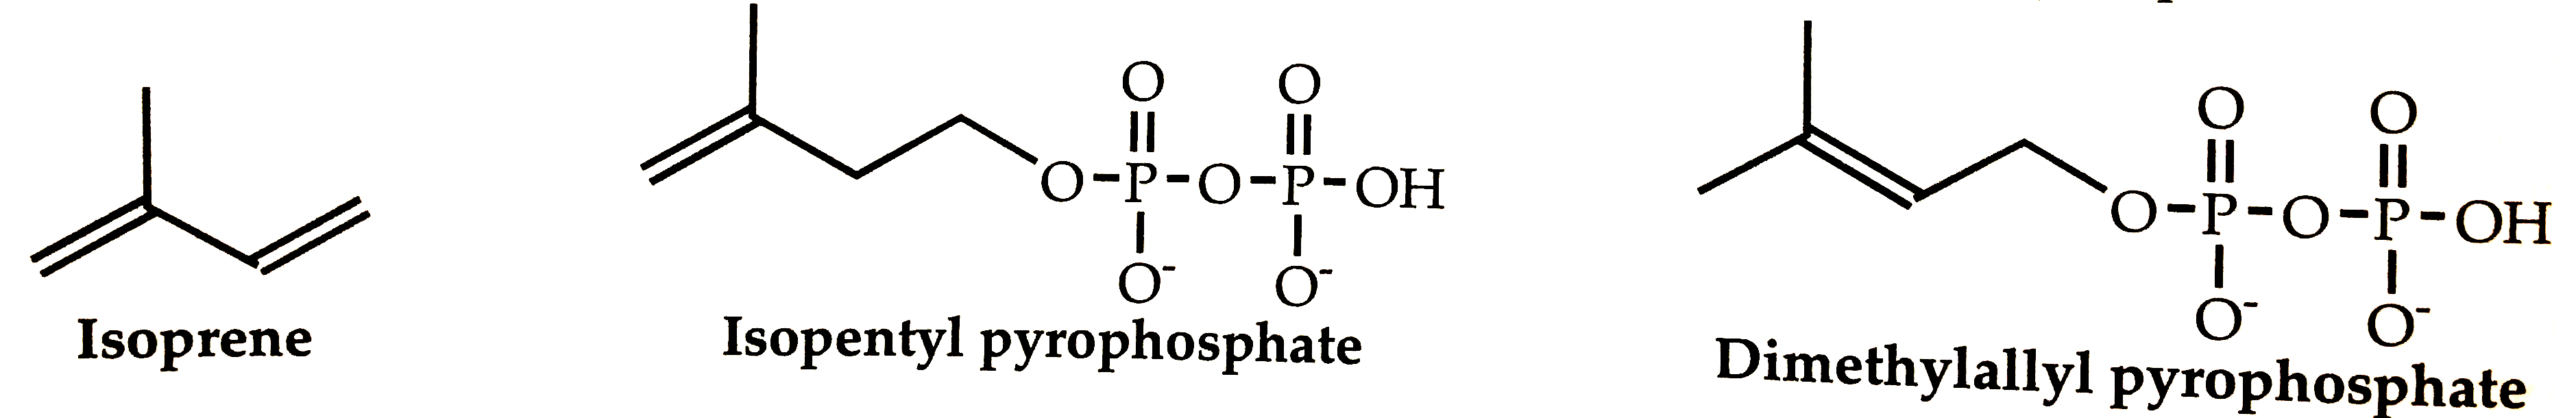
\includegraphics[width=0.75\textwidth]{isoprene.png} \label{isoprene}
\caption{The chemical structures of isoprene, isopentenyl pyrophosphate, and dimethylallyl pyrophosphate.}
\end{figure}
\indent The synthesis of cholesterol involves terpenes and terpinoids, even though cholesterol itself is not a terpene. As a general rule, smaller terpenes are found primarily in plants, while some larger terpenes like lanesterol and $\beta$-carotene are found in both plants and animals. One of the skills that you must develop to do well on terpene-related questions on the MCAT is to recognize terpenes and be able to identify the isoprene subunits in the carbon skeleton. \textbf{Fig. \ref{terpenes}} shows the analysis of some terpenes for the isoprene units in the skeletal fragments. \\
\begin{figure}[!ht]
\centering
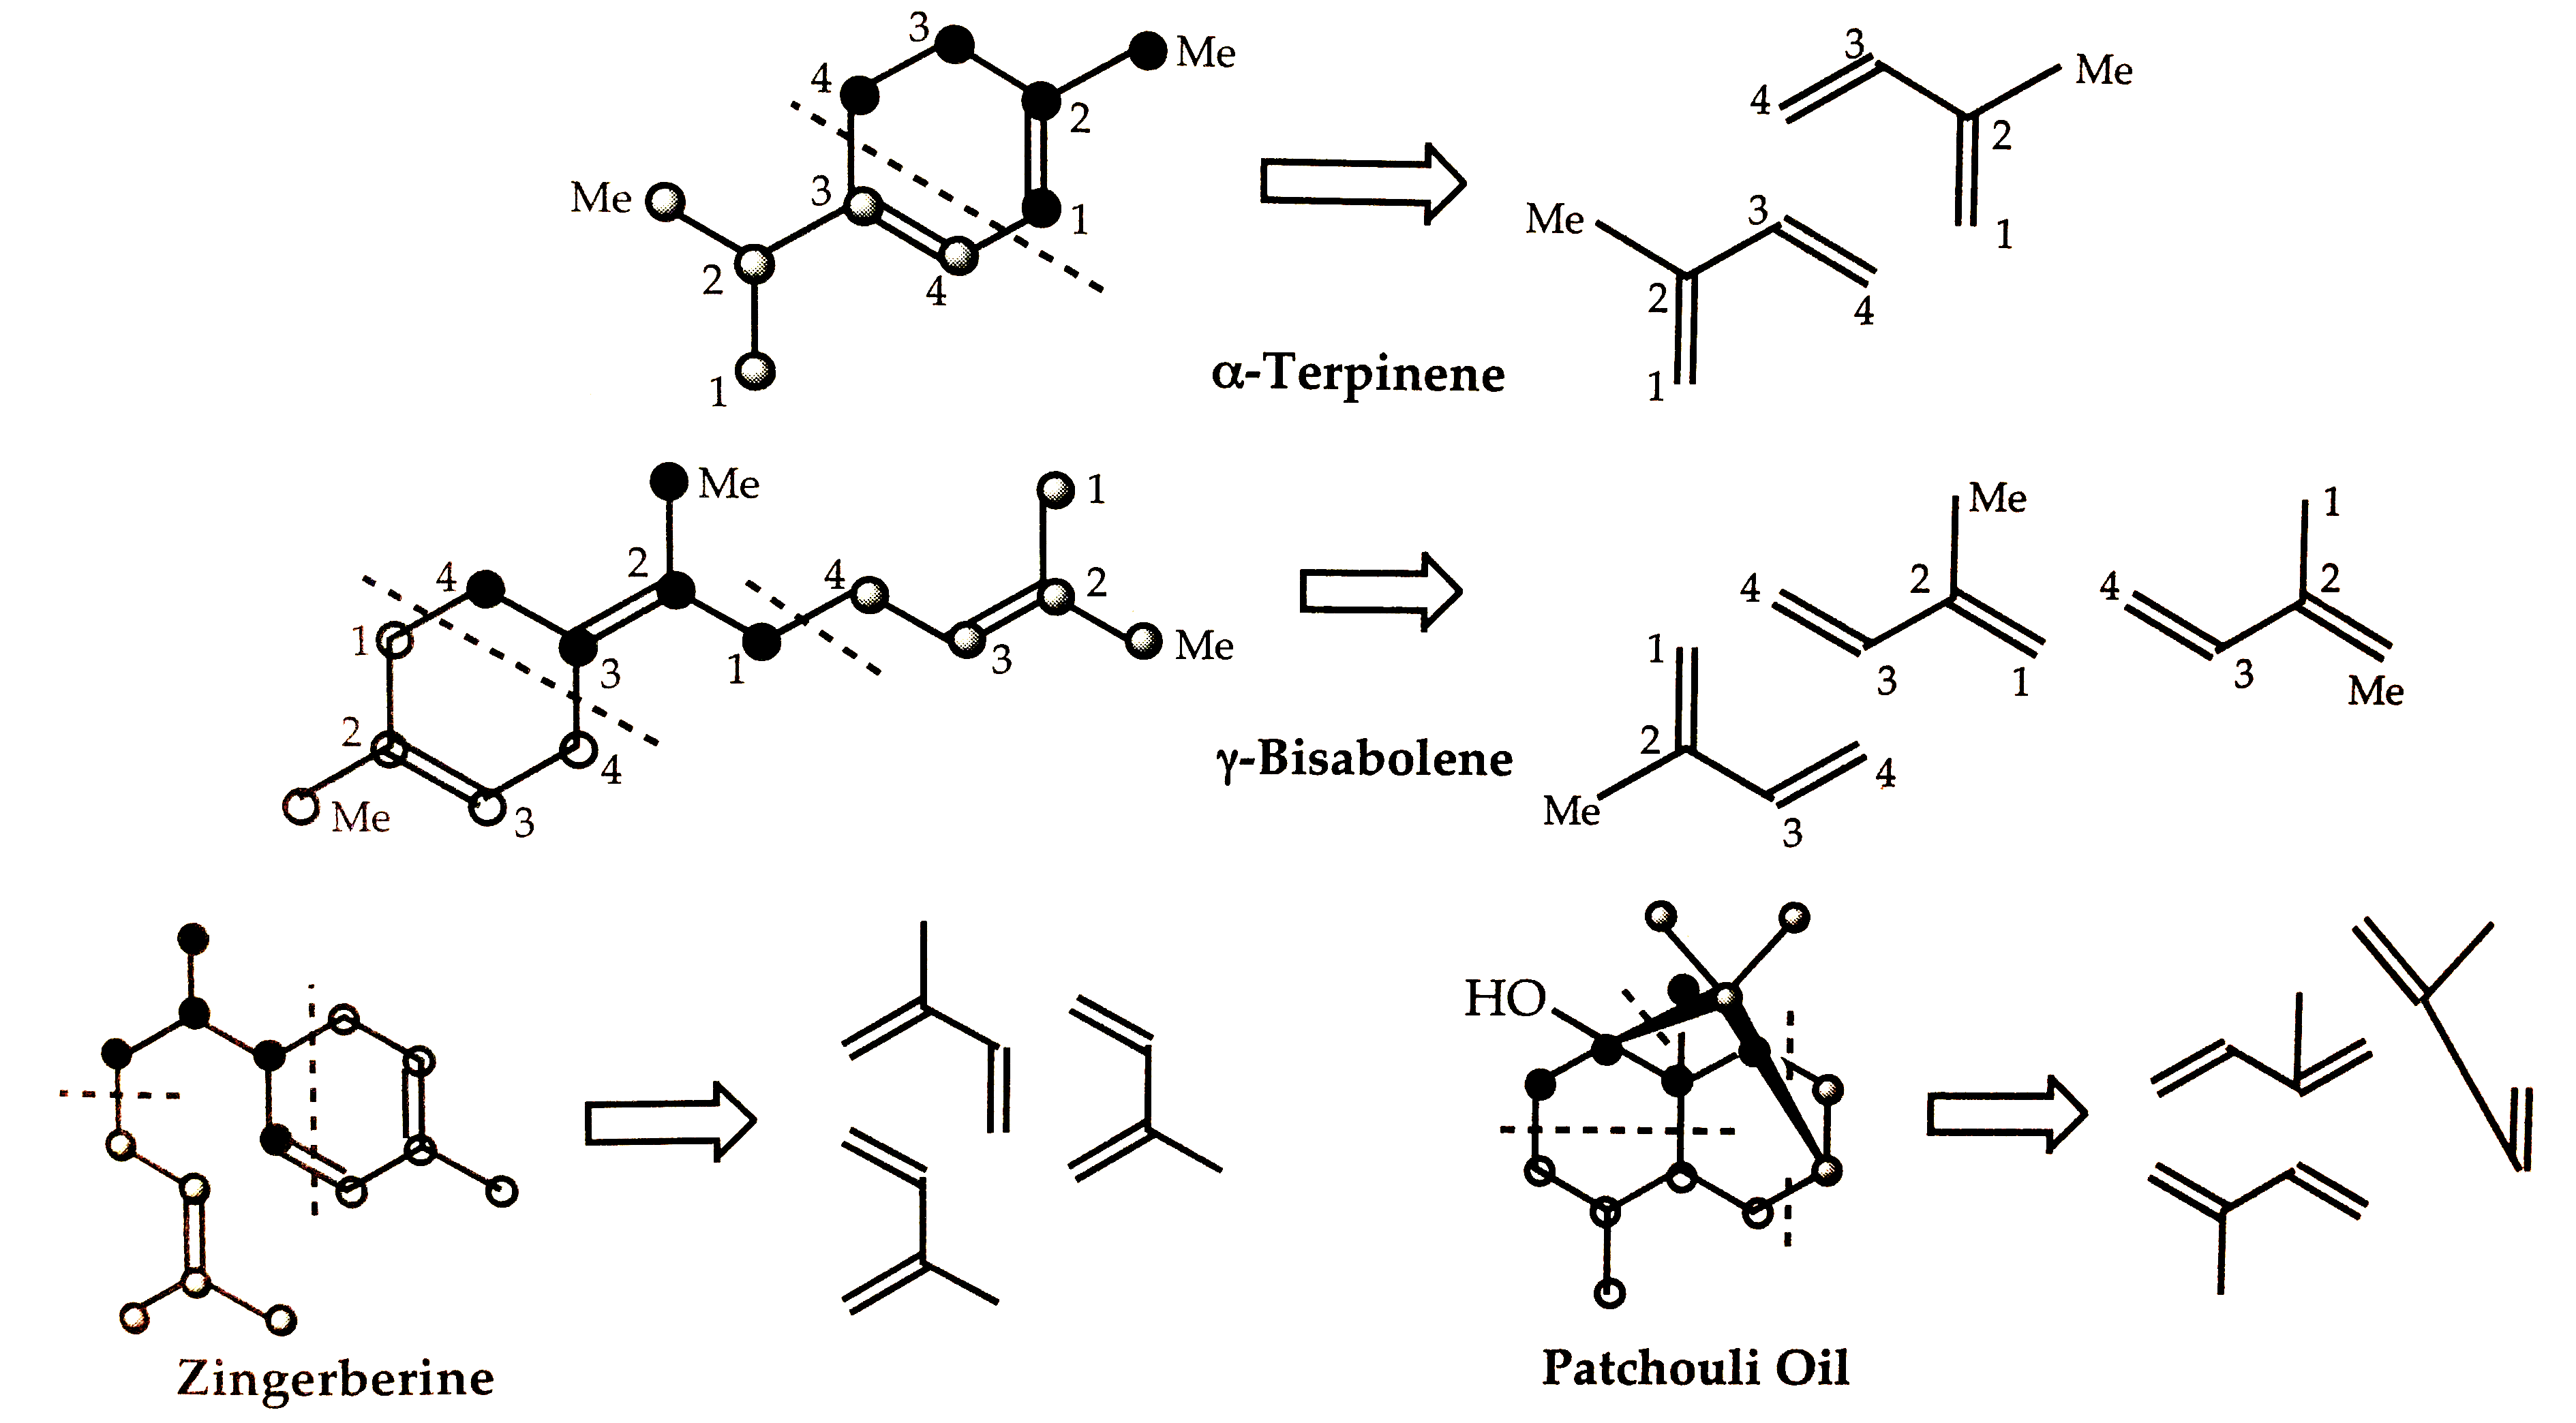
\includegraphics[width=0.7\textwidth]{terpenes.png} \label{terpenes}
\caption{Identifying terpenes for their isoprene units in the skeletal fragments.}
\end{figure}
\indent Terpenes are UV-active, because of their $\pi$-bonds and conjugated system. As the degree of conjugation increases, both the intensity and $\lambda_{max}$ increase. A common lab technique employed to isolate terpenes is \textit{steam distillation}, where the pulp of a natural material is placed into water and boild so that the natural oils are distilled from the pulp. This allows the essential oils to vaporize at a temperature lower than their boiling point, so they do not degrade. The distillate is a mixture of water and terpenes, which are easily separated using extraction techniques. Terpenes can also be extracted from pulp. When isolating terpenes, it is often a mixture of geometrical isomers that is collected. The different isomers of a terpene are given the prefixes $\alpha$-, $\beta$-, $\gamma$-, and so on. The different geometrical isomers have similar physical properties, but because of differences in conjugation, they exhibit differences in the absorption of UV-visible photons. \\
\indent Terpenes are often isolated in educational laboratory experiments. Because of their biological significance and the fact they are isolated in lab experiments, they are represented on the MCAT. If you have a fundamental understanding of terpenes, then you should be fine. Here is an example problem involving terpenes:
\begin{center}
\begin{minipage}{30em}
\textcolor{blue}{Which of the following compounds is NOT a terpene or terpenoid? See \textbf{Fig. \ref{5_13}} for the answer choices.}
\end{minipage}
\end{center}
\noindent Terpenes are built from 5-carbon subunits, which means that they should contain a carbon total that is a multiple of five. Choice \textbf{D} has sixteen carbons, so it cannot be a terpene or terpenoid.
\begin{figure}[!ht]
\centering
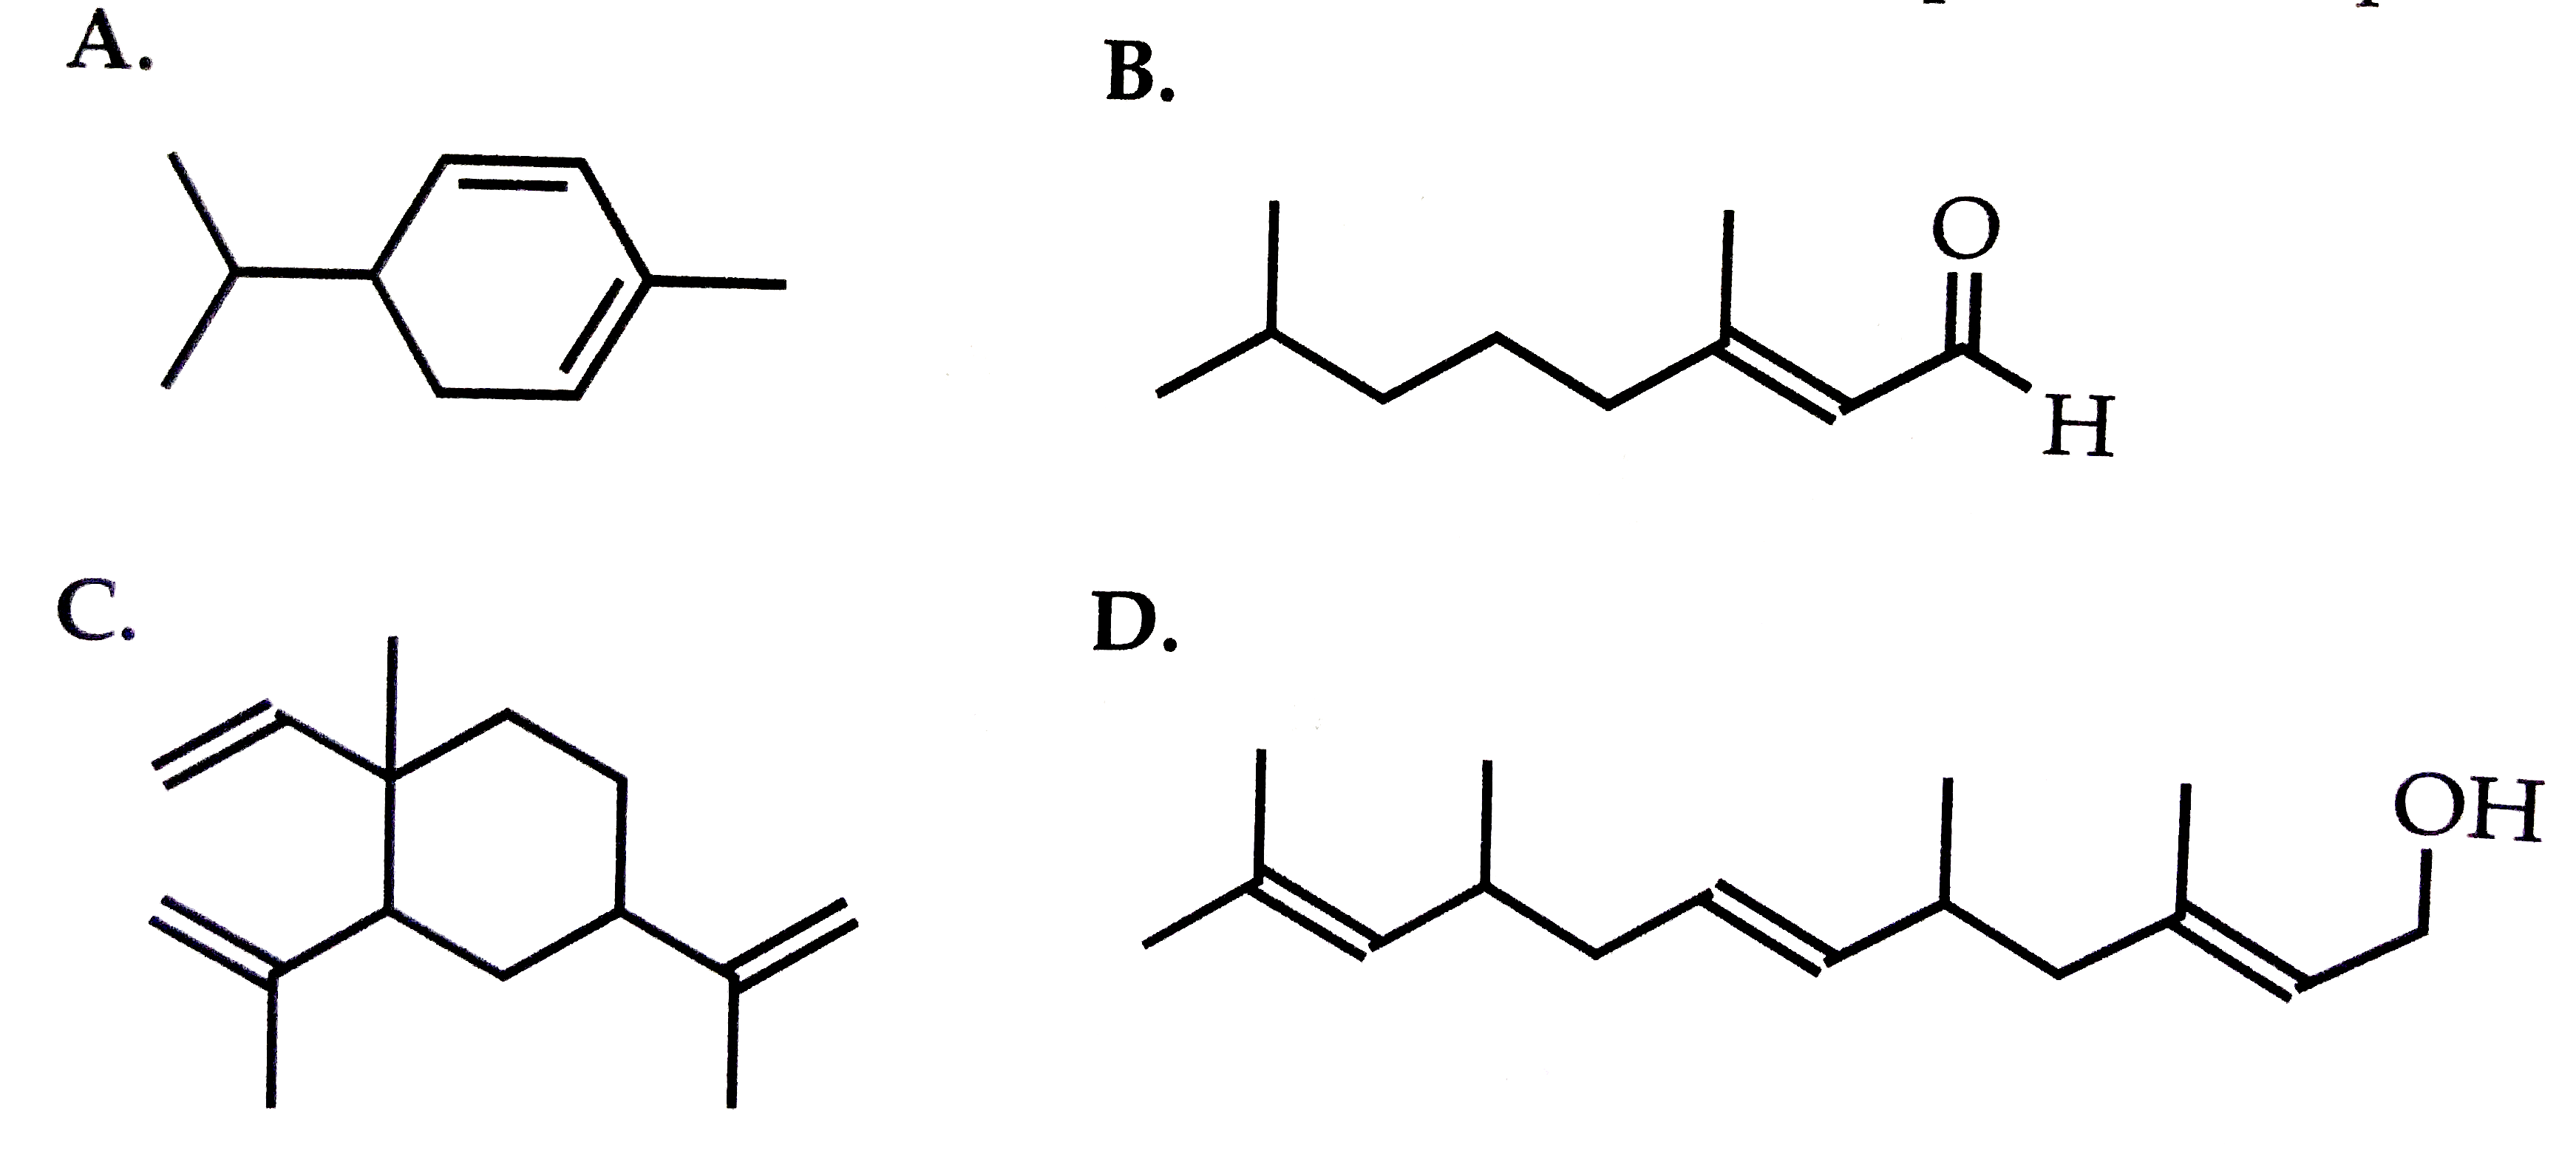
\includegraphics[width=0.6\textwidth]{5_13.png} \label{5_13}
\caption{Identifying terpenes for their isoprene units in the skeletal fragments.}
\end{figure}

\subsection{General Bioorganic Reactions}
There's no way you can memorize all of the reactions that can be tested on the MCAT, so we choose to present classes of reactions you should know, and in doing so will present some specific examples that hopefully seem familiar. You should recognize (1) substitution reactions where a nucleophile displaces a leaving group from carbon (covered previously in Nucleophilic Substitution section of Organic Chemistry), (2) addition reactions where two groups (an electrophile and nucleophile) add to the two neighboring carbons of a $\pi$-bonds, (3) electrocyclic reactions reactions where $\pi$-bonds and rings are formed or broken in a concerted fashion, (4) redox reactions where carbons gain and/or lose bonds to hydrogen and oxygen, and finally (5) free-radical reactions where carbon is electron deficient and thus highly reactive. The examples in this section will have biological application to show that the approach can also help with biochemistry as well as organic chemistry.\\
\indent Reactions with alkenes are common in biochemistry. You should be familiar with hydrogenation, dehydrogenation, hydration, and dehydration. \textbf{Fig. \ref{alkene_reactions}} shows two simple biochemical reactions of alkenes.\\
\begin{figure}[!ht]
\centering
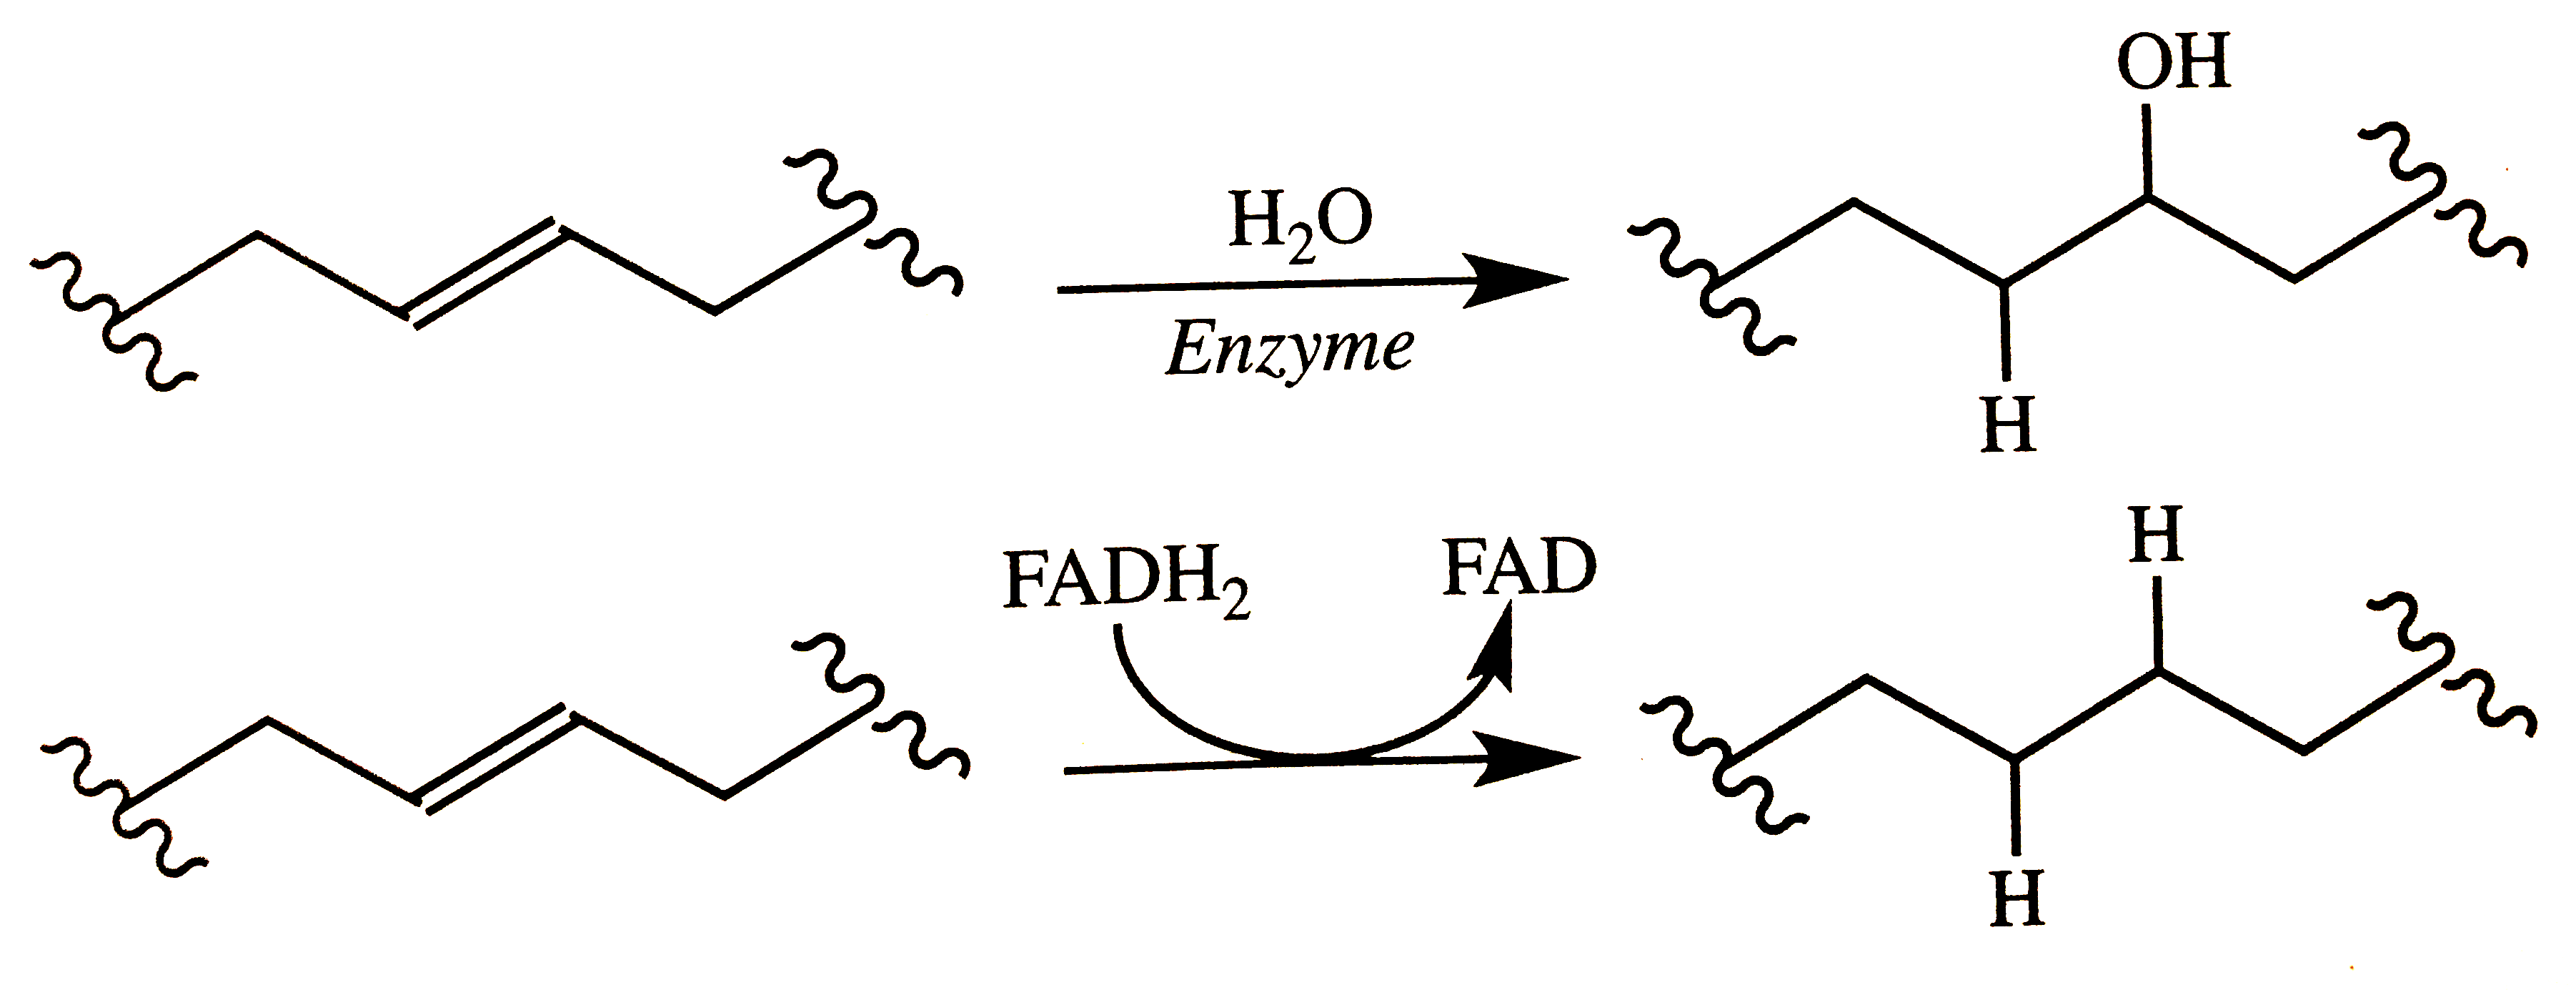
\includegraphics[width=0.6\textwidth]{alkene_reactions.png} \label{alkene_reactions}
\caption{Biochemical examples of alkene addition reactions.}
\end{figure}
\indent \textit{Pericyclic reactions} involve the repositioning of $\sigma$-bonds and $\pi$-bonds. through a cyclic transition state. These reactions are believed to be concerted, meaning that the formation and breaking of all bonds occur simultaneously. Pericyclic reactions include cycloaddition reactions, sigmatropic rearrangement, and electrocyclic reactions. In cycloaddition, two separate compounds come together, resulting in a single new compound. In sigmatropic rearrangement reactions, it is an intramolecular rearrangement that takes place. An electrocyclic addition reaction involves the addition of a conjugated diene (with 4 $\pi$-electrons) to an alkene (with 2 $\pi$-electrons) to form a six-membered ring. The transition state is similar to the resonance of benzene, as shown in \textbf{Fig. \ref{electrocyclic}}. These operations can be both ring closing and ring opening.\\
\begin{figure}[!ht]
\centering
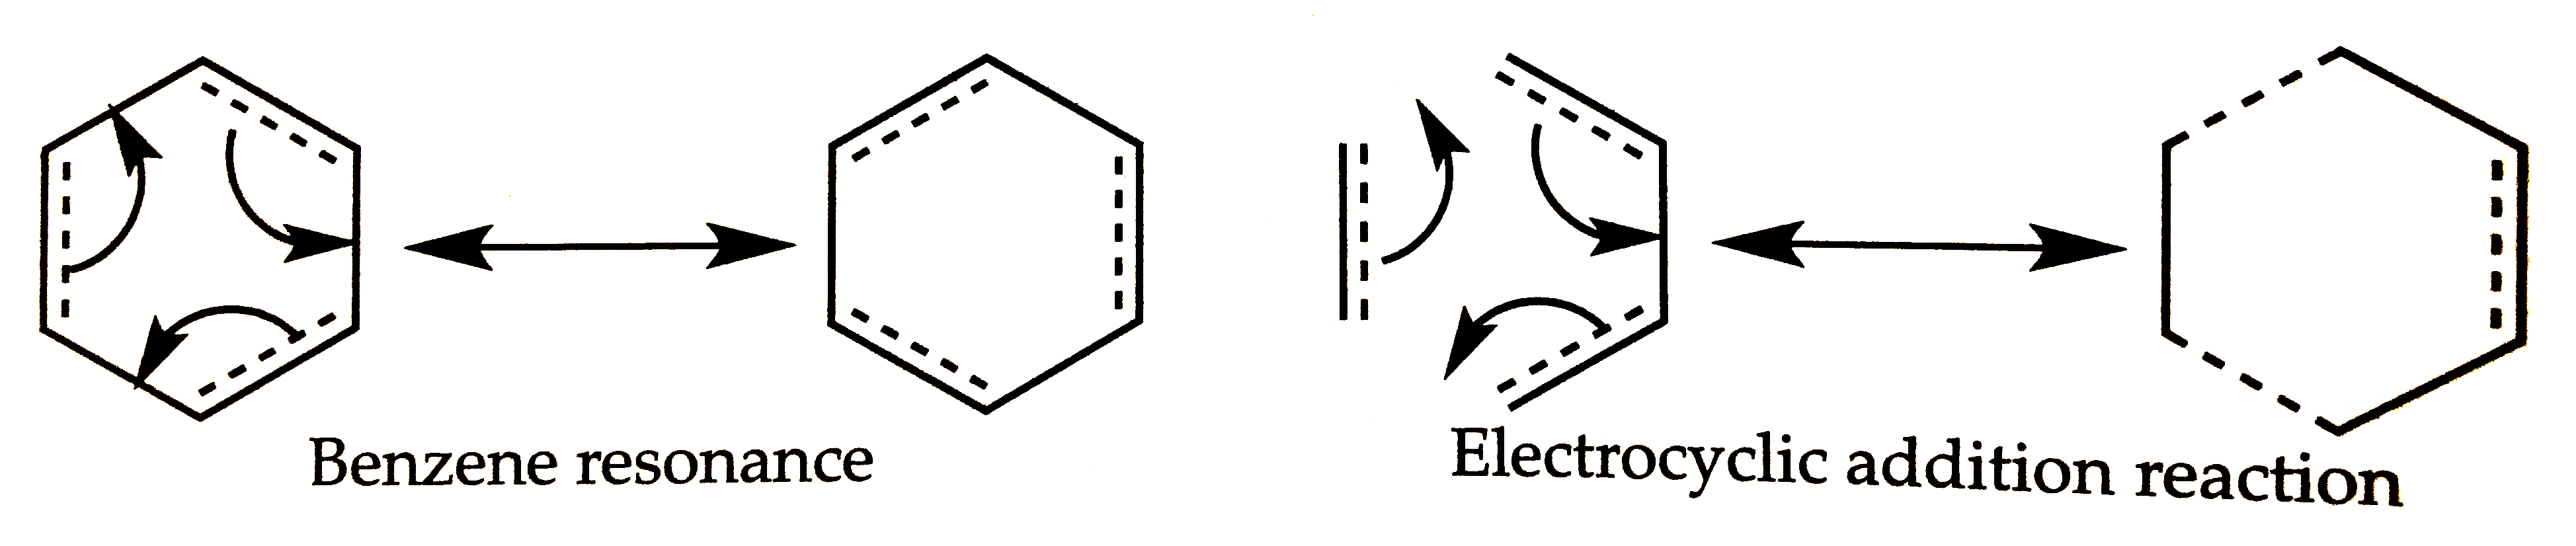
\includegraphics[width=0.6\textwidth]{electrocyclic.png} \label{electrocyclic}
\caption{An example of an electrocyclic addition reaction. Notice its similarity to the resonance of benzene.}
\end{figure}
\indent Biochemical redox reactions are also a common reaction type in biological systems. Examples include dehydrogenation, reactions involving \ce{NADH}, \ce{NADPH}, or \ce{FAD}, and reactions involving methyl transfers.

\subsection{Carbonyls and Alcohols}
\textbf{Fig. \ref{carbonyls}} shows several types of carbonyl compounds and carbonyl derivatives. More generally, oxygen-containing compounds tested on the MCAT include carbonyls, carbonyl derivatives, and alcohols. Because of their ability to form hydrogen bonds, alcohols typically have high boiling points and are generally miscible in water. Alcohols are not good nucleophiles, but they can be deprotonated and converted into an \textit{alkoxide} (the deprotonated form of an alcohol) under basic conditions. Because alkoxides are strong bases, they are not an ideal nucleophile, but they are generally better than alcohols. Alcohol chemistry also involves oxidation of the hydroxyl group into a carbonyl group. Alcohols can also be formed from the reduction of carbonyls. On \ce{{}^1H} NMR, the \ce{-OH} group does not couple well, so we rarely consider splitting patterns for alcohols. The \ce{-OH} peak also slowly disappears with the addition of \ce{D_2O} to the NMR tube. \\
\begin{figure}[!ht]
\centering
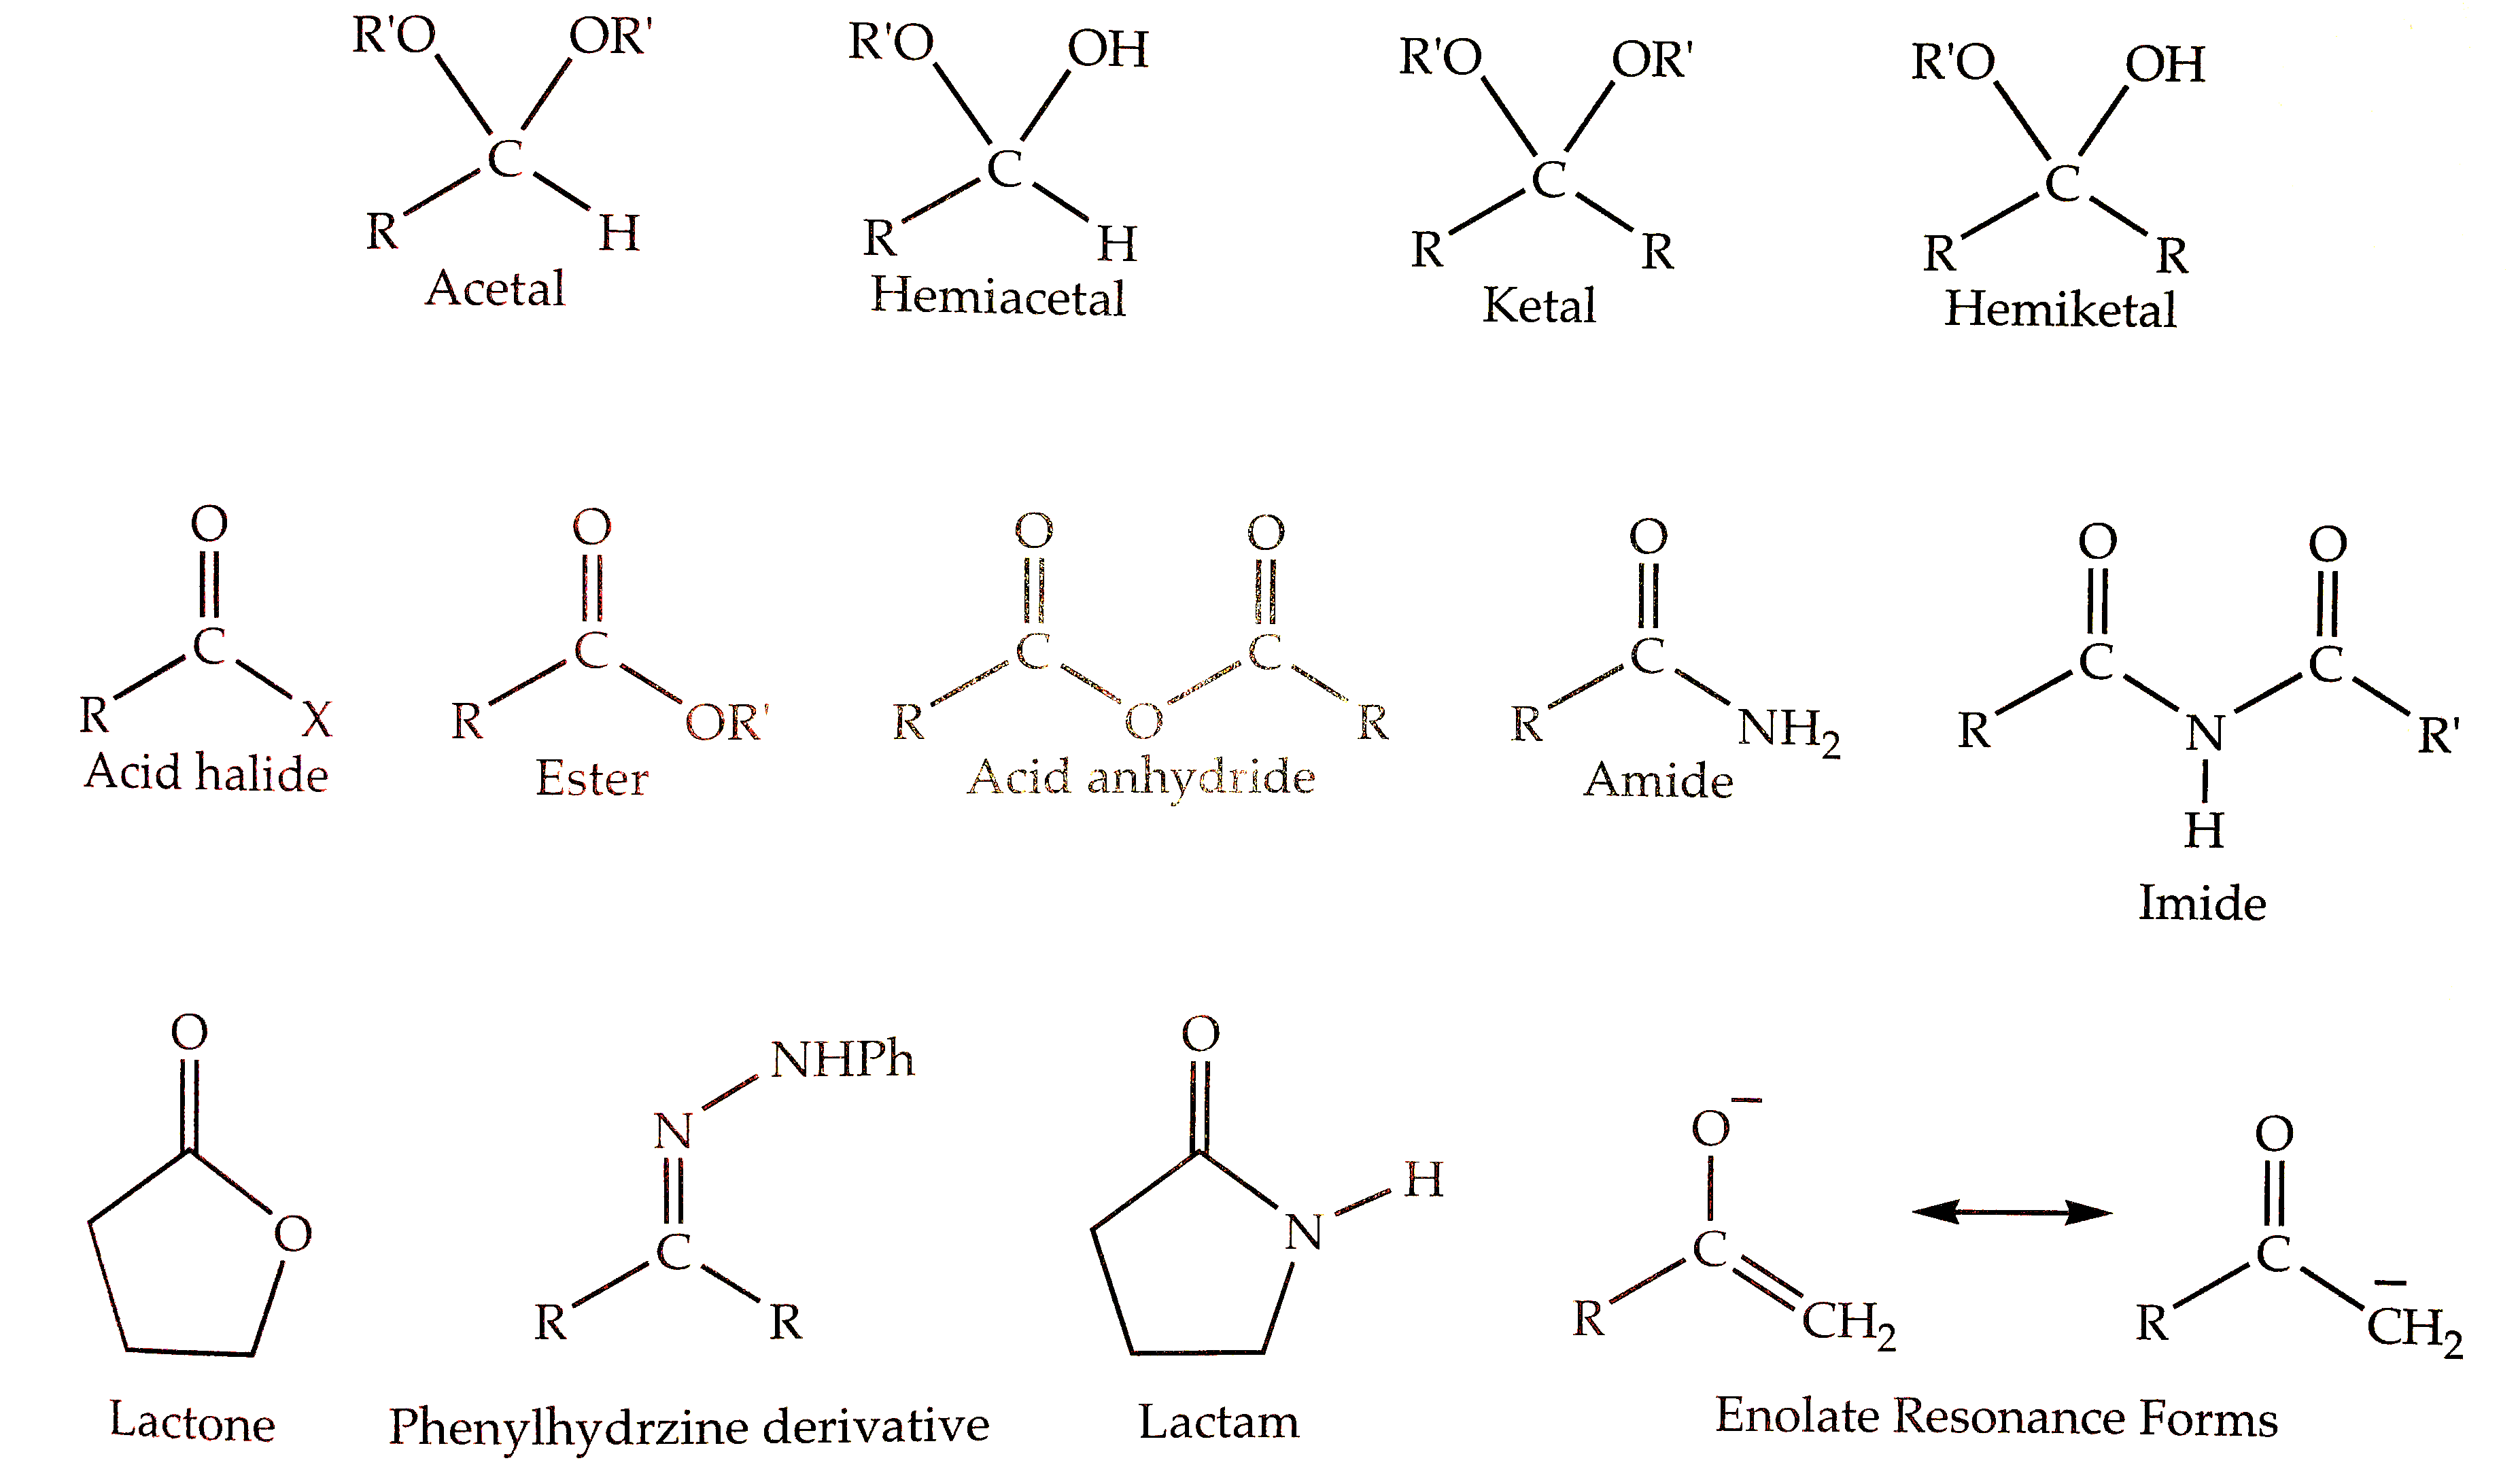
\includegraphics[width=0.7\textwidth]{carbonyls.png} \label{carbonyls}
\caption{Selected carbonyl compounds and their derivatives.}
\end{figure}
\indent Because aldehydes and ketones do not form hydrogen bonds, they typically have boiling points only \textit{slightly} higher than alkanes of equal mass. Because of the polarity of the carbonyl bond, they are slightly miscible in water. The reactivity of aldehydes and ketones occurs primarily at the electrophilic carbonyl center. Aldehydes and ketones are reactive with most nucleophiles, but not by a `traditional' nucleophilic substitution mechanism. Once a nucleophile attacks a carbonyl carbon, it forms a four-ligand intermediate with a negative charge on oxygen known as a \textit{tetrahedral intermediate}. The chemistry of aldehydes is similar to the chemistry of ketones, except that an aldehyde can by oxidized into a carboxylic acid while ketones cannot be oxidized easily. \\
\indent \textbf{Ketals} and \textbf{hemiketals} are derivatives of ketones while \textbf{acetals} and \textbf{hemiacetals} are derivatives of aldehydes. Ketals occur when a ketone loses the carbonyl group and gains two alkoxy \ce{R-O} functional groups. Notice that the oxidation state of carbon doesn't change. A hemiketal occurs when the ketone has its carbonyl group converted into a hydroxyl group and gains one alkoxy group. Acetals are similar to ketals, except it is the aldehyde that loses its carbonyl group to gain the two alkoxy groups. Hemiacetals are similar to hemiketals, except it again is an aldehyde, rather than a ketone, that converts its carbonyl group into a hydroxyl group while gaining an alkoxy group. \textbf{Fig. \ref{ketals_acetals}} shows the formation of these four compounds. \\
\begin{figure}[!ht]
\centering
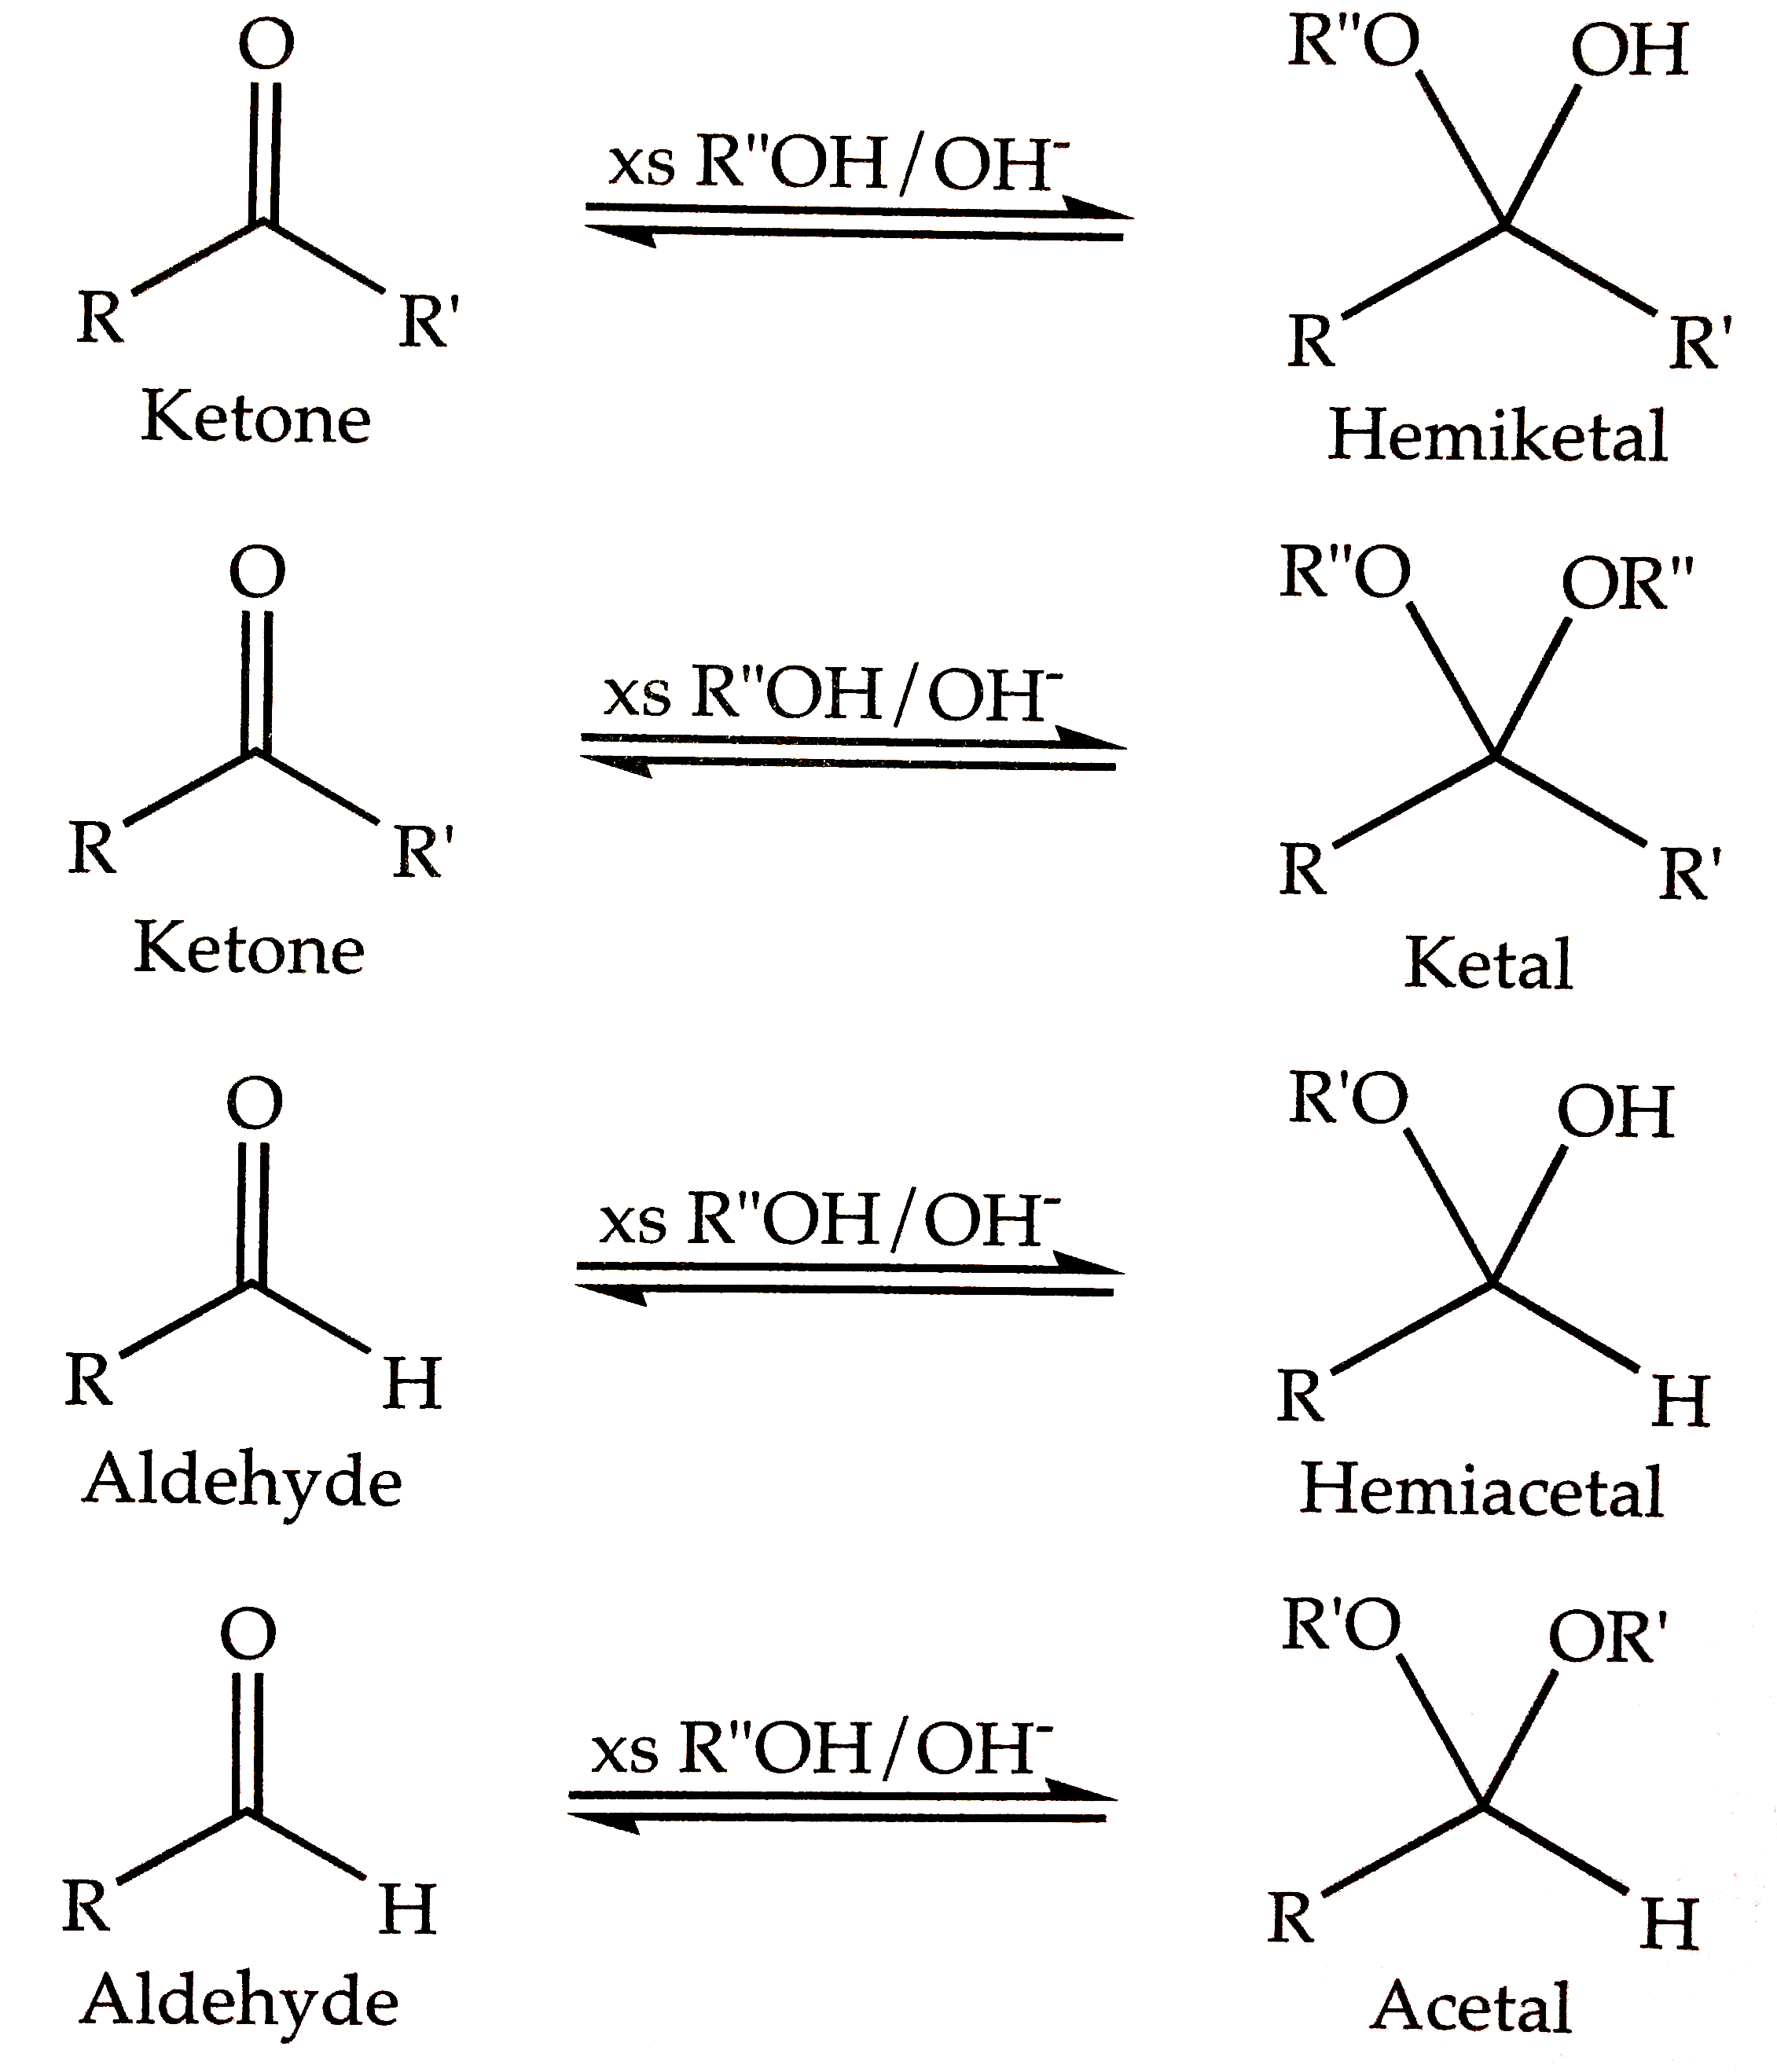
\includegraphics[width=0.4\textwidth]{ketals_acetals.png} \label{ketals_acetals}
\caption{Formation of ketals, hemiketals, acetals, and hemiacetals.}
\end{figure}
\indent Ketals and acetals serve as protecting groups for carbonyl groups in synthesis involving ketones and aldehydes. Hemiacetals and hemiketals are not useful as protecting groups, but they are important in sugar chemistry. Acetals and ketals can be formed and removed only under acidic conditions, where as hemiacetals and hemiketals are formed only under basic conditions but removed under any conditions. \textbf{Fig. \ref{ketal_mechanism}} shows the mechanism for formation of a ketal from a ketone under acidic conditions. It is the same mechanism for the formation of an acetal from an aldehyde, except that an aldehyde is the reactant, rather than a ketone. Meanwhile, \textbf{Fig. \ref{hemiacetal_mechanism}} shows the formation of a hemiacetal from an aldehyde and alcohol in the presence of a strong base. These mechanisms should be kept as simplistic as possible.\\
\begin{figure}[!ht]
\centering
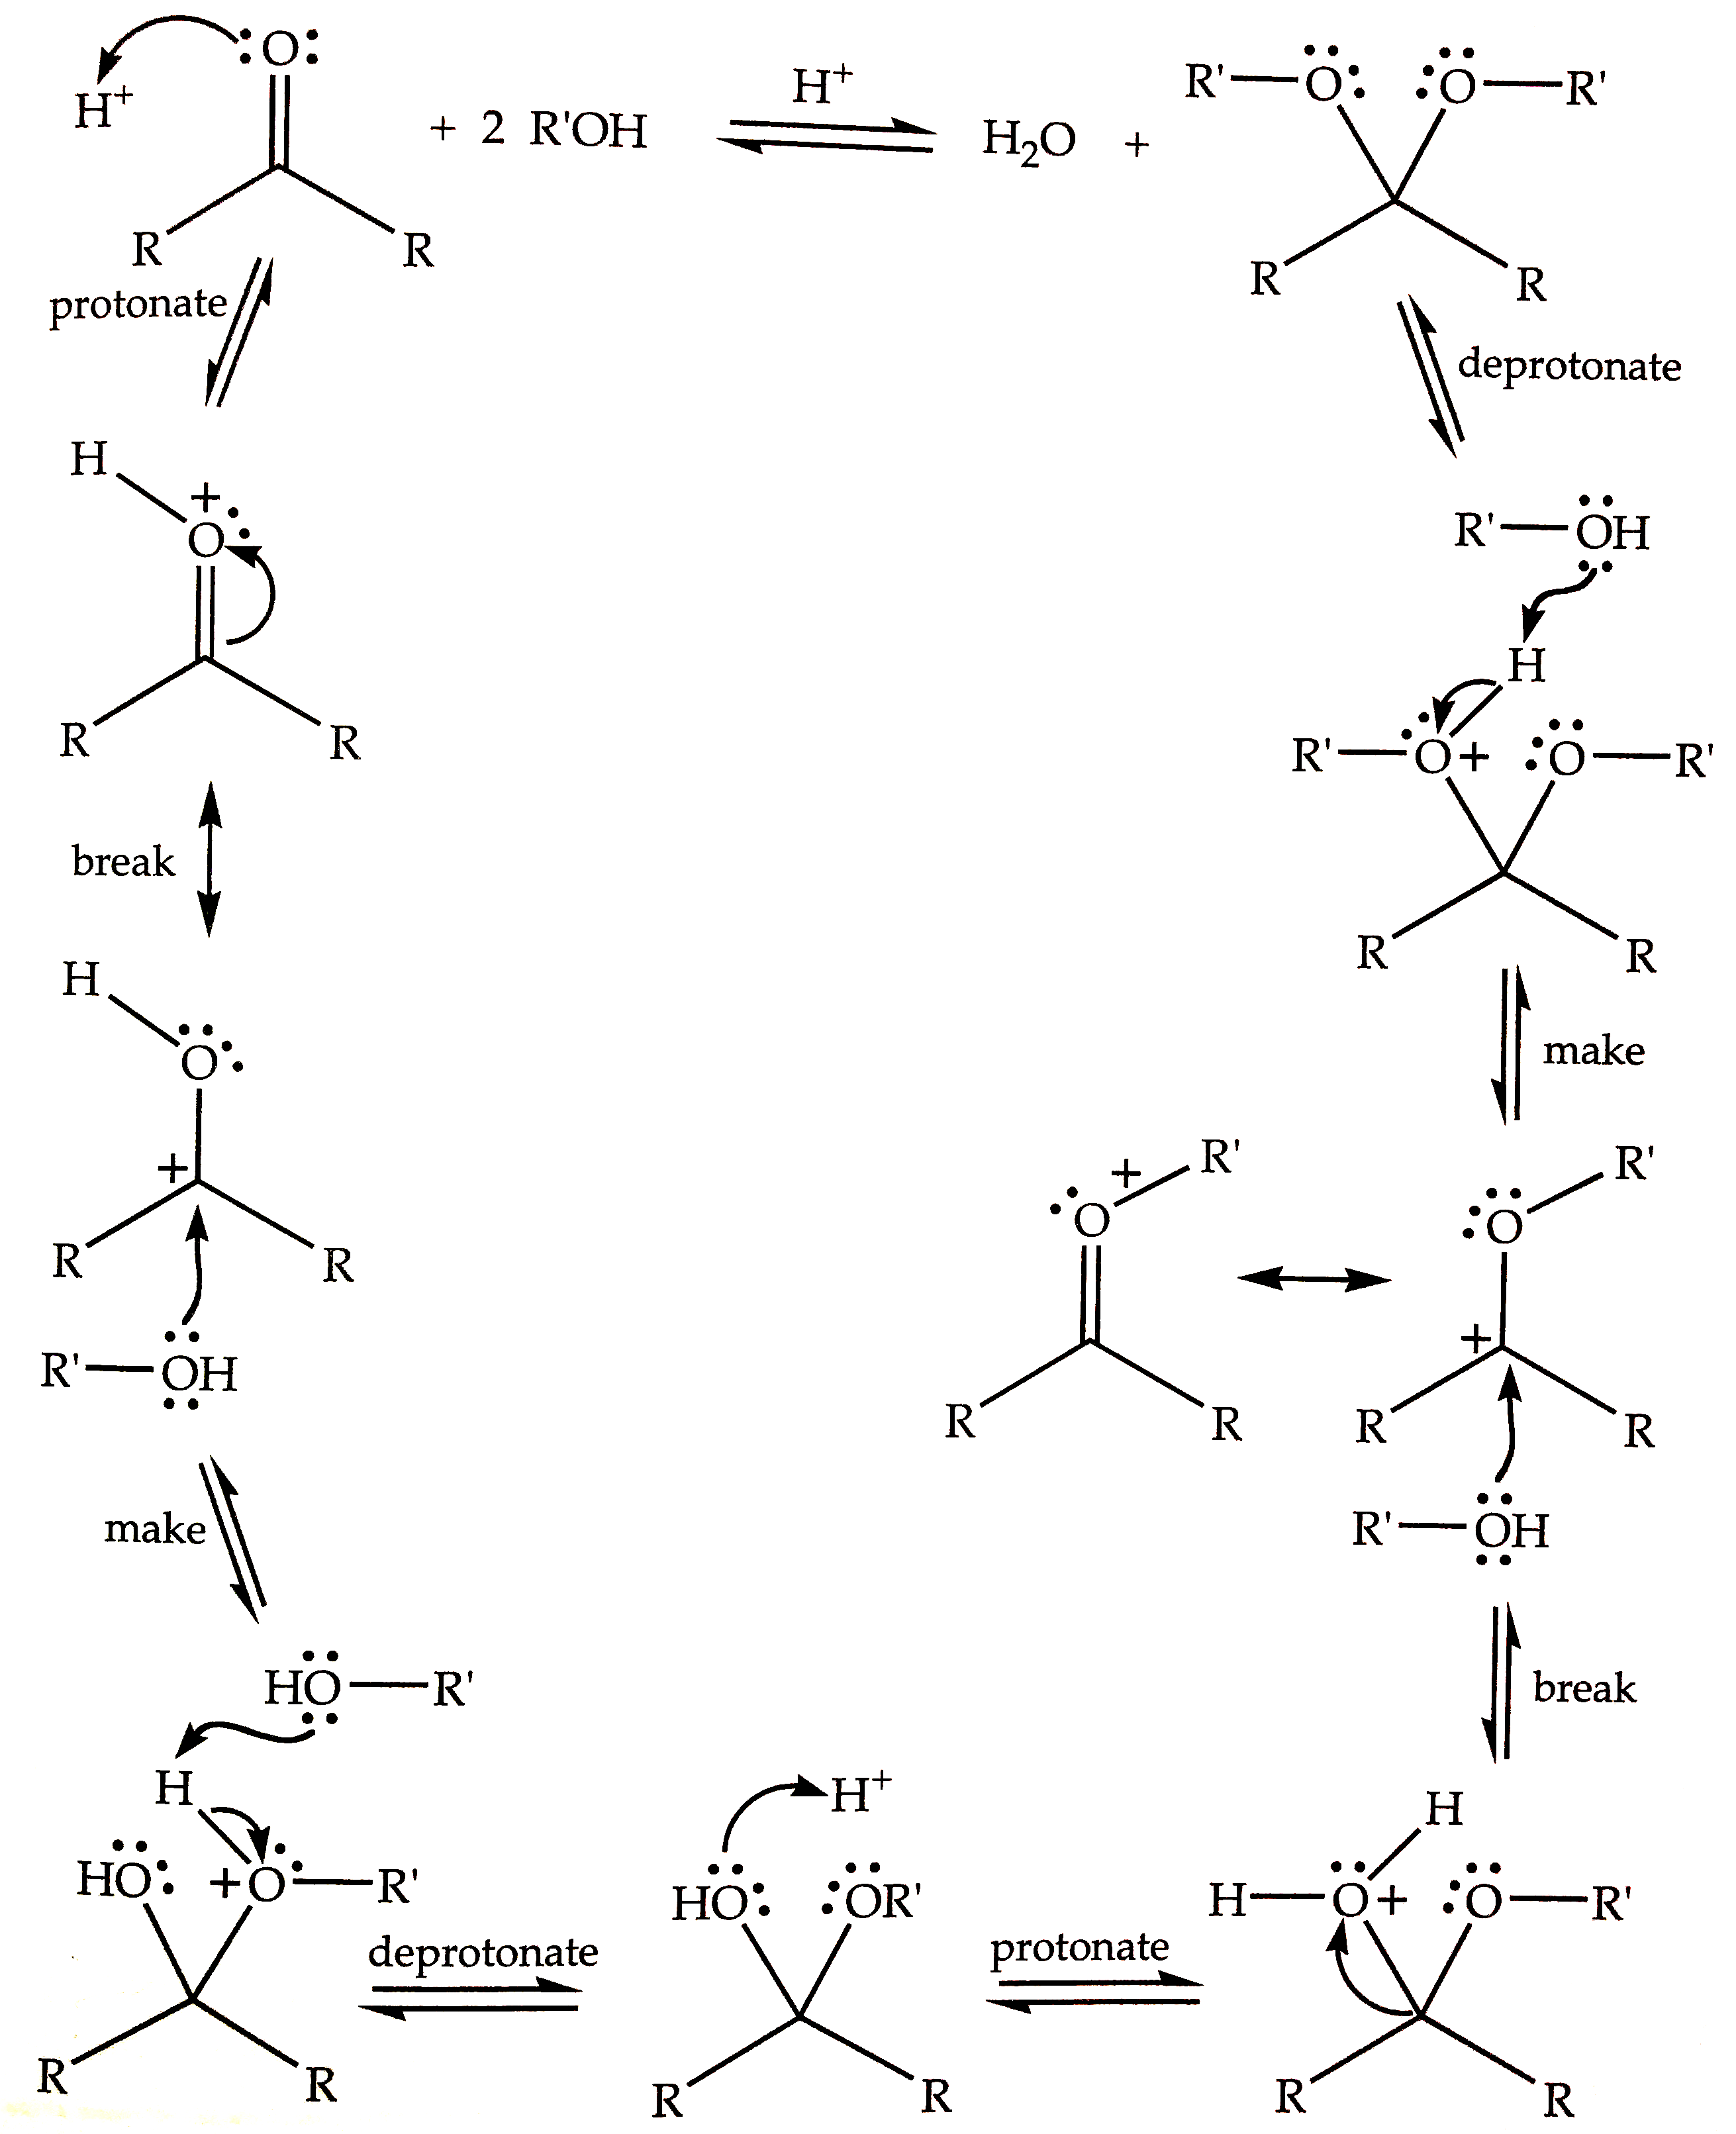
\includegraphics[width=0.4\textwidth]{ketal_mechanism.png} \label{ketal_mechanism}
\caption{Mechanism for the formation of a ketal from an ketone under acidic conditions.}
\end{figure}
\begin{figure}[!ht]
\centering
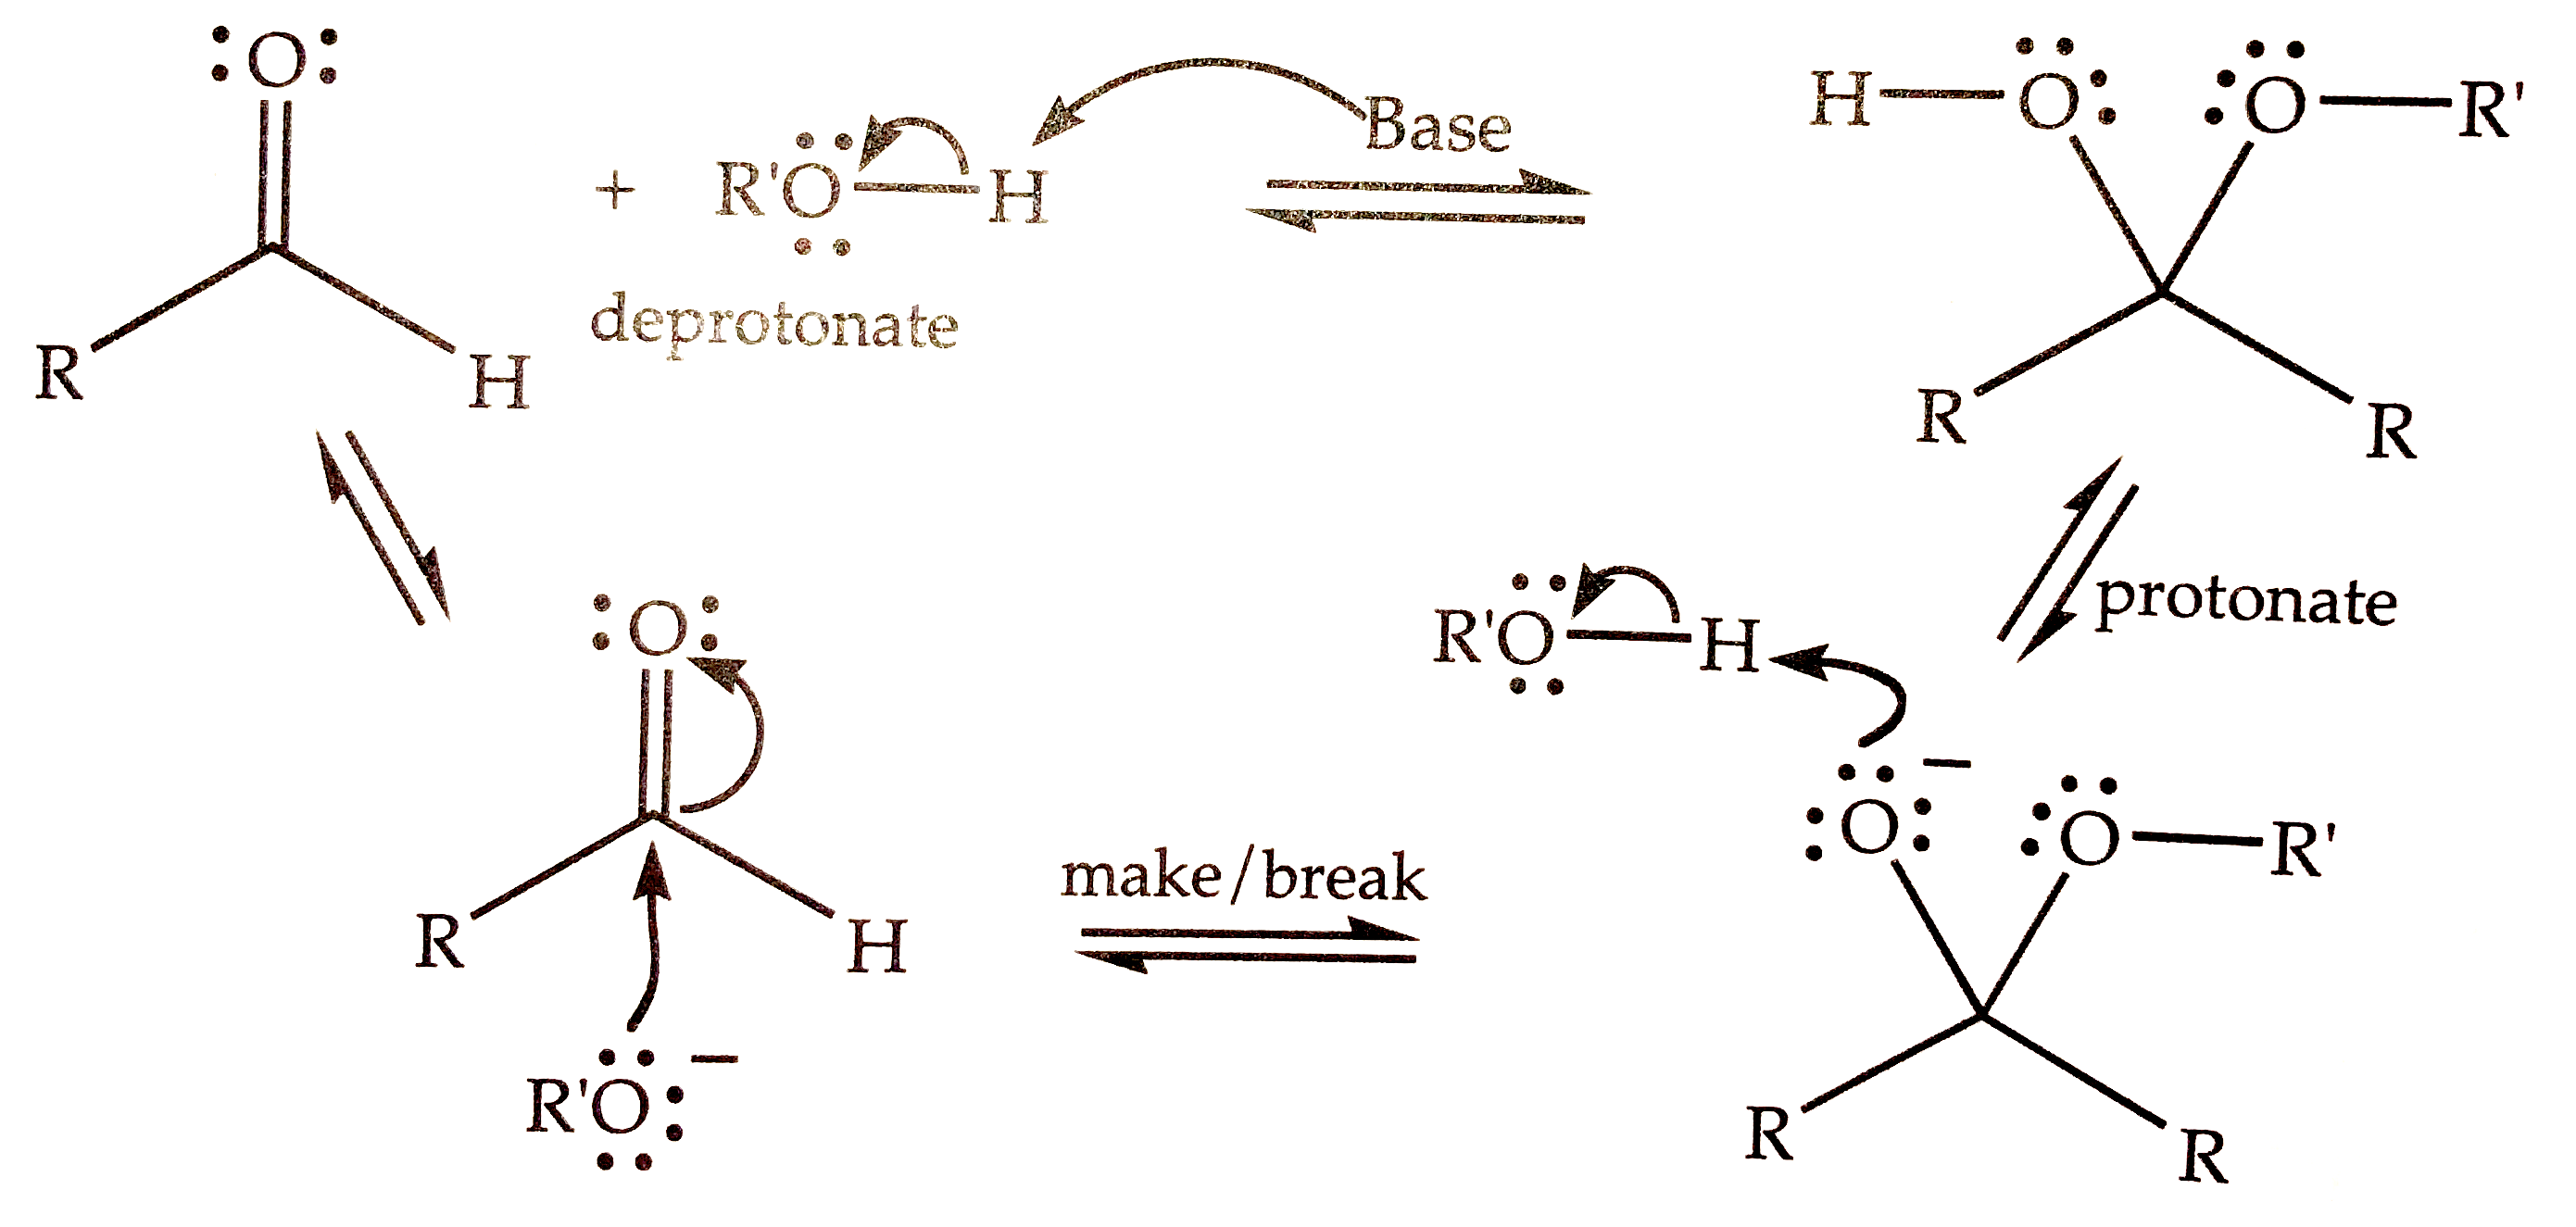
\includegraphics[width=0.65\textwidth]{hemiacetal_mechanism.png} \label{hemiacetal_mechanism}
\caption{Mechanism for the formation of a hemiacetal from an aldehyde and alcohol in the presence of strong base.}
\end{figure}
\indent \textbf{Protecting groups} are used in synthesis to prevent a reagent from reacting at a site where it is undesirable to have a reaction. Aldehydes and ketones employ the same reaction to add the same protecting group, forming either an acetal or ketal. Because acetals and ketals are less reactive than aldehydes and ketones, they are an ideal protecting group. The alcohol that is typically used to form the protected carbonyl compound is a vincinal diol (a 1,2-diol), such as ethylene glycol (\ce{HOCH_2CH_2OH}). \textbf{Fig. \ref{protecting}} shows the protecting of cyclohexanone using ethylene glycol. As a guideline, any time that you have a molecule with more than one reactive site, you must protect the sites at which you wish to have no reaction. The exception to this rule is when the site you wish to react is significantly more reactive than any other sites on the molecule. \\
\begin{figure}[!ht]
\centering
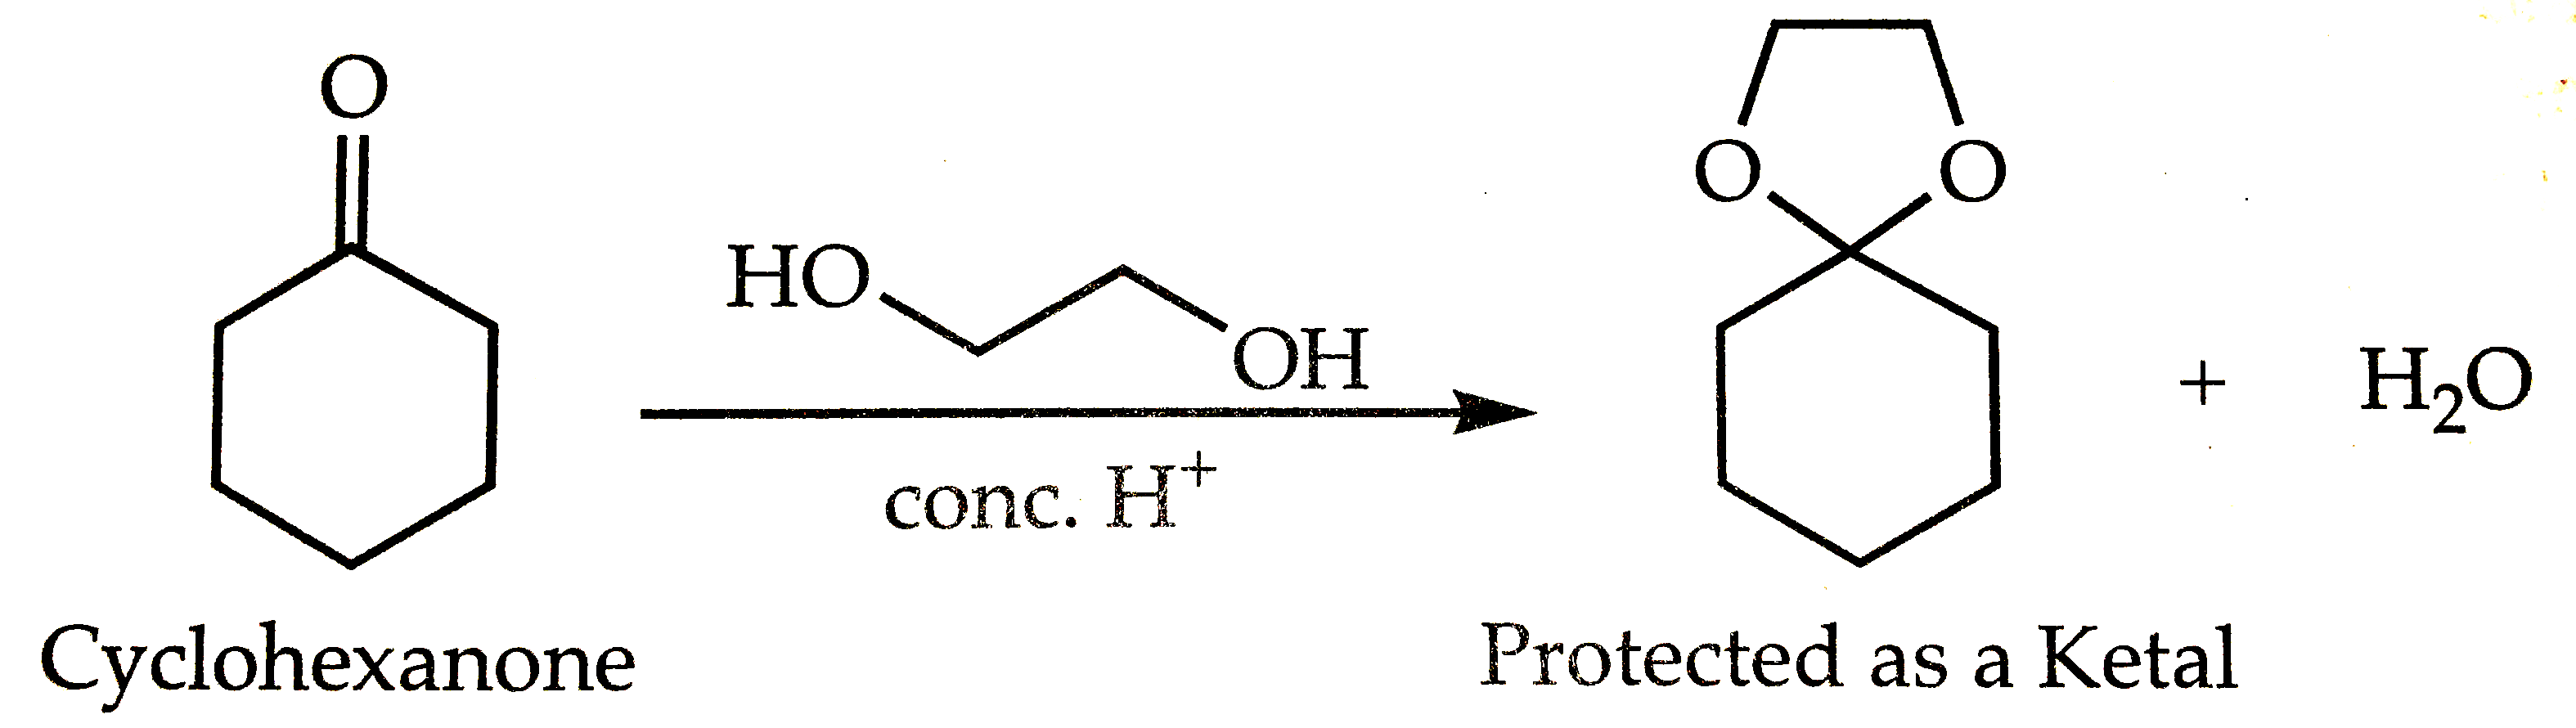
\includegraphics[width=0.65\textwidth]{protecting.png} \label{protecting}
\caption{Ketals and acetals as protecting groups.}
\end{figure}
\indent Unlike aldehydes and ketones, \textbf{carboxylic acid derivatives} have a functional group. that potentially can act as a leaving group. Carboxylic acids can be converted into esters, anhydrides, or acid halides. Carboxylic acids can be formed by \textit{saponification} (i.e. treating an ester with strong base in water), by treating a methyl ketone with \ce{I_2} and a strong base, by oxidizing primary alcohols and. aldehydes in water, or by hydrolyzing a nitrile or an amide using strong acid at high temperatures. These reactions are shown in \textbf{Fig. \ref{acid_source}}. Carboxylic acids can also be reduced into primary alcohols or converted into other compounds such as acid halides, acid anhydrides, or esters. \textbf{Fig. \ref{acid_derivatives}} shows four reactions of carboxylic acids with which you are expected to be familiar with. \\
\begin{figure}[!ht]
\centering
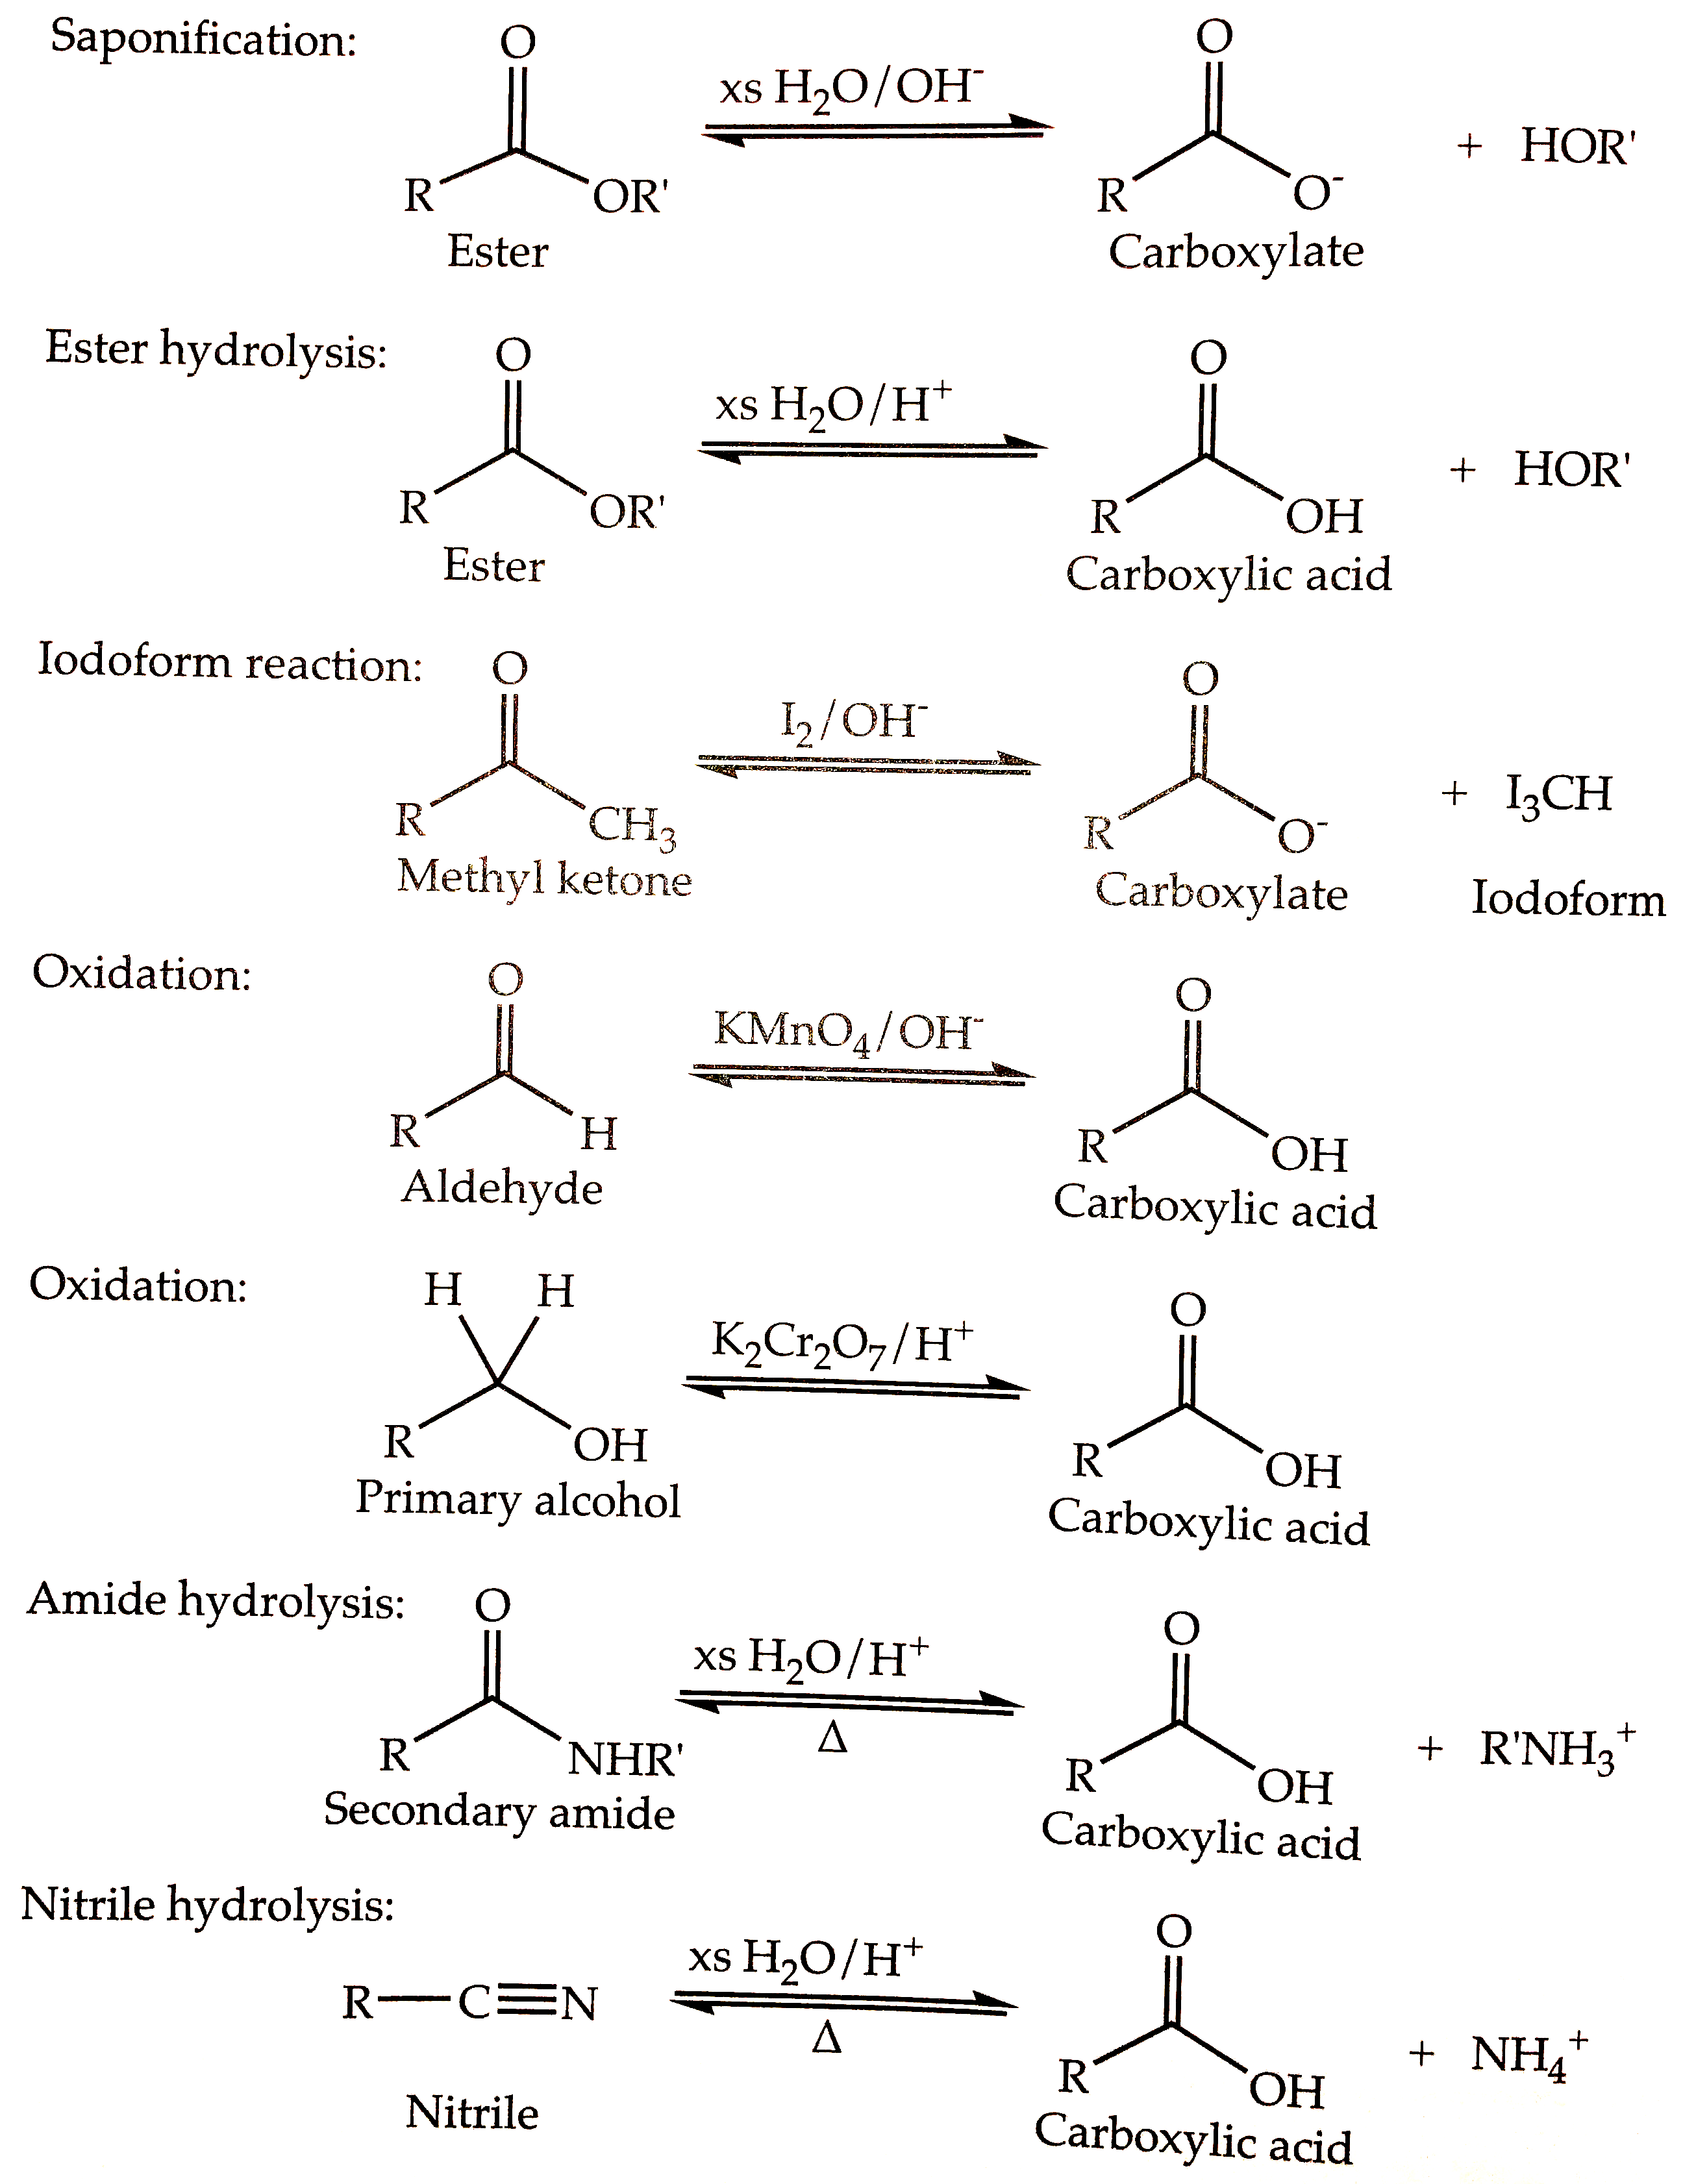
\includegraphics[width=0.5\textwidth]{acid_source.png} \label{acid_source}
\caption{Different formation reactions for carboxylic acids.}
\end{figure}
\begin{figure}[!ht]
\centering
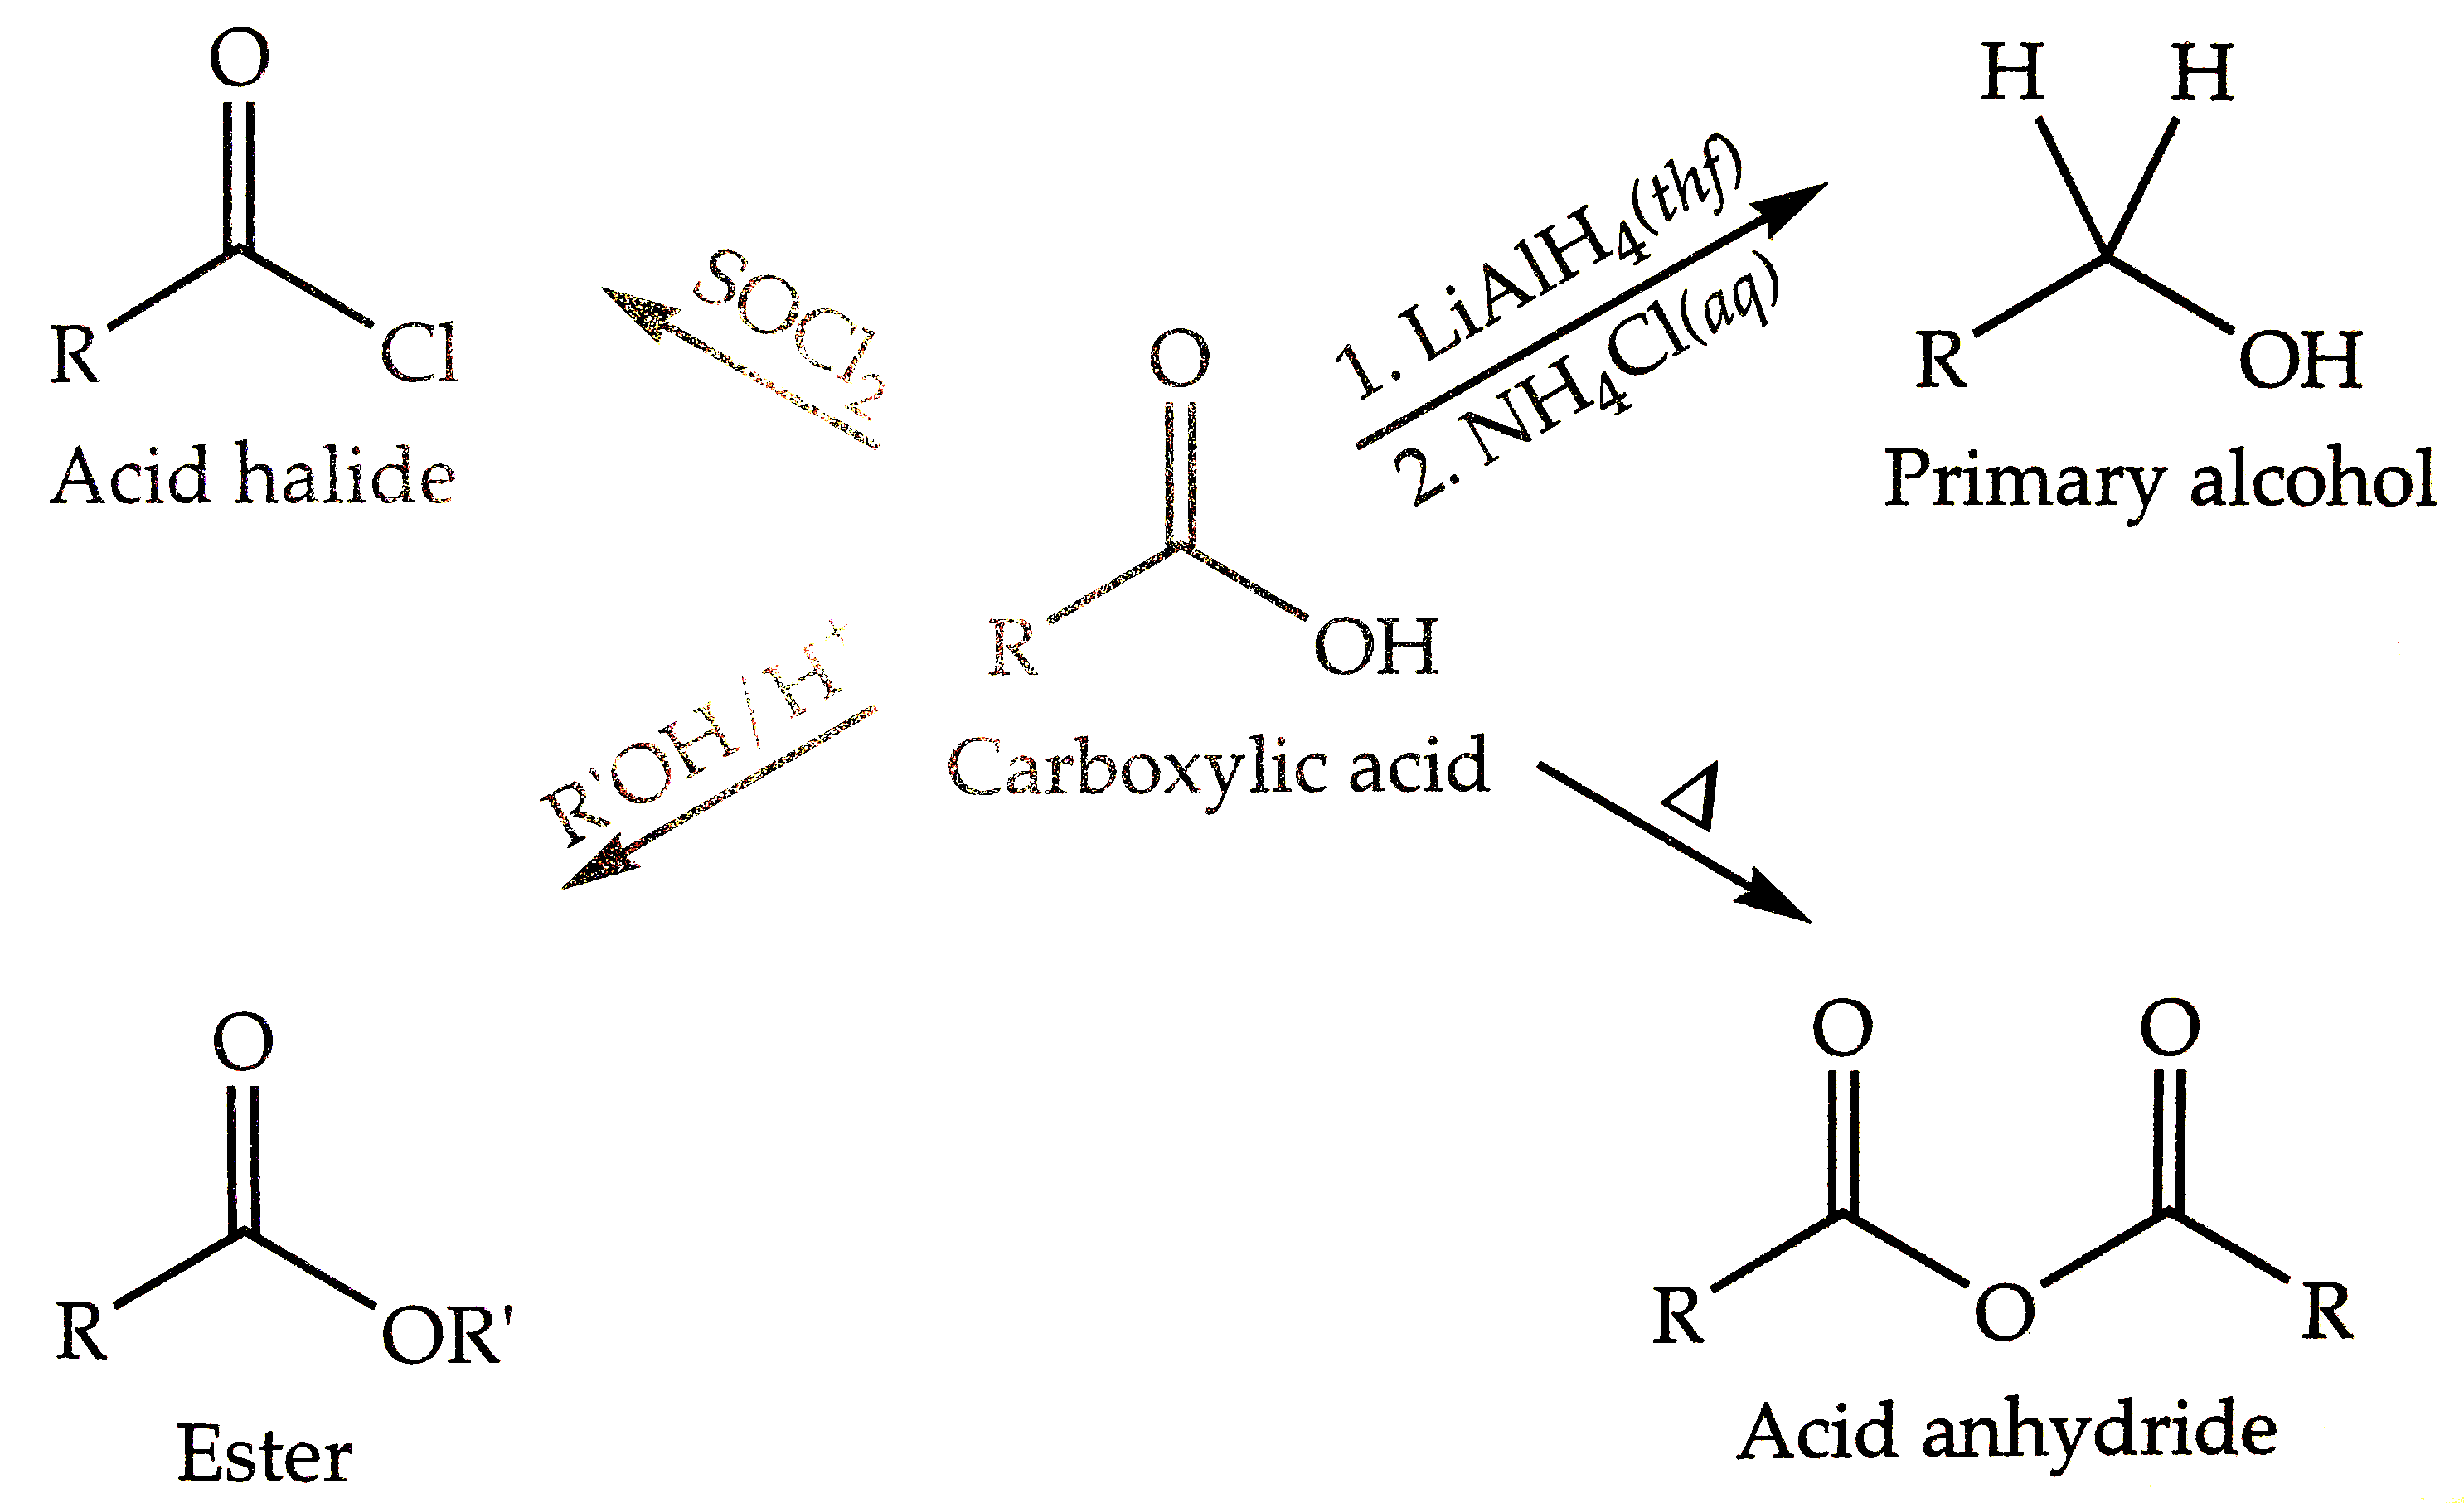
\includegraphics[width=0.65\textwidth]{acid_derivatives.png} \label{acid_derivatives}
\caption{Four reactions of carboxylic acids with which you are expected to be familiar.}
\end{figure}
\indent \textbf{Esters} are carbonyl compounds with an alkyl group and an alkoxy group attached to the carbonyl carbon. Esters have a leaving group (i.e. the alkoxy group), so they undergo more reactions than ketones or aldehydes. Esters can exchange their alkoxy group in the presence of acid and an alcohol in what is referred to as a \textit{transesterification reaction}. \\
\indent \textbf{Lactones} are cyclic esters. They can be synthesized by treating cyclic ketones with peroxyacids (\ce{RCO_3H}) in what is known as the \textit{Baeyer-Villiger} reaction. \textbf{Fig. \ref{lactone}} shows the formation of a lactone from an intramolecular transesterification reaction of a hydroxyester. \\
\begin{figure}[!ht]
\centering
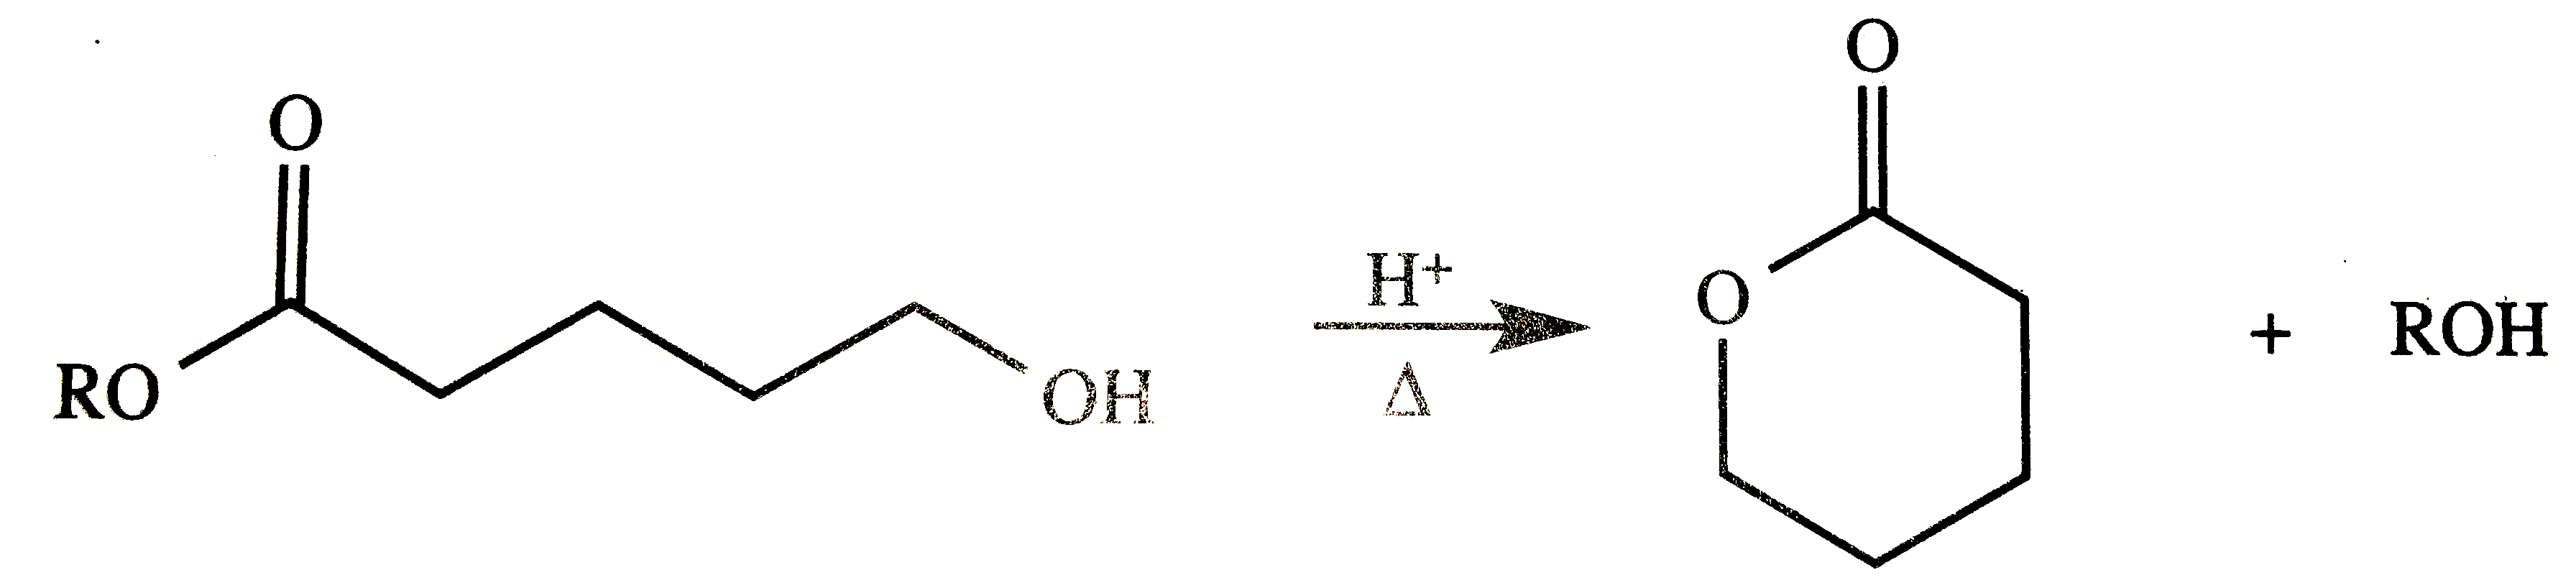
\includegraphics[width=0.65\textwidth]{lactone.png} \label{lactone}
\caption{Formation of a lactone from an intramolecular transesterification reaction of a hydroxyester.}
\end{figure}
\indent \textbf{Acid anhydrides} are formed by a condensation reaction of two carboxylic acids at high temperature. Therefore, when you add water to an acid anhydride, it breaks into two carboxylic acids.\\
\indent \textbf{Acid halies} are similar to esters, but with a halide (\ce{Cl}, \ce{Br}, or \ce{I}) in place of the alkoxy group. They are the most reactive of all the carbonyl compounds, because the halide is a great leaving group. They undergo the same substitution reactions as other carbonyl compounds that have a leaving group, but they react faster.\\
\indent \textbf{Amides} are carbonyls with an amine group bonded to the carbonyl carbon. Amides form the backbone of proteins, and they are found in most of the bases of nucleic acids. An amide bond that links amino acids together is referred to as a \textit{peptide bond}. Amides can be reduced into amines using a strong reducing agent, such as \ce{LiAlH_4}.

\subsection{Carbonyl Reactivity}
Because carbonyl compounds contain a \ce{C=O} bond, they are good electrophiles. The difference in reactivity between a ketone and a carboxylic acid derivative, such as an ester, centers around the presence of a leaving group on the carbonyl carbon. A \textit{tetrahedral intermediate} is formed when a carbonyl compound is attacked by a nucleophile. For carbonyl compounds that have leaving groups, the reactivity of the carbonyl compound is based on the strength of the leaving group\textemdash stronger leaving groups make for a more reactive (more electrophilic) carbonyl compound. For example, an acid halide can easily be converted into an anhydride, ester, or amide. An acid anhydride can readily be converted into an ester or amide, but it is hard to convert the anhydride into an acid halide. \\
\indent The hydrogen on the $\alpha$ carbon (the carbon adjacent to the carbonyl carbon) is mildly acidic, so a strong base can remove it. \textbf{Enolates} form when a hydrogen on the $\alpha$ carbon is deprotonated. The enolate can gain a proton at the oxygen, forming an \textbf{enol}. A ketone and enol are \textbf{tautomers} (structural isomers that vary in the position of a $\pi$-bond and a hydrogen), so the conversion from a ketone into its enol is known as \textit{tautomerization}, as shown in \textbf{Fig. \ref{tautomerization}}. The $\alpha$ carbanion that results when an \ce{H} is stripped by a strong base is a good nucleophile, so when an alkyl halide is added to the solution, the carbanion can attack the alkyl halide in a nucleophilic substitution reaction to form a new carbon-carbon bond. This results in a longer ketone. The generic reaction is shown in \textbf{Fig. \ref{longer_ketone}}. \\
\begin{figure}[!ht]
\centering
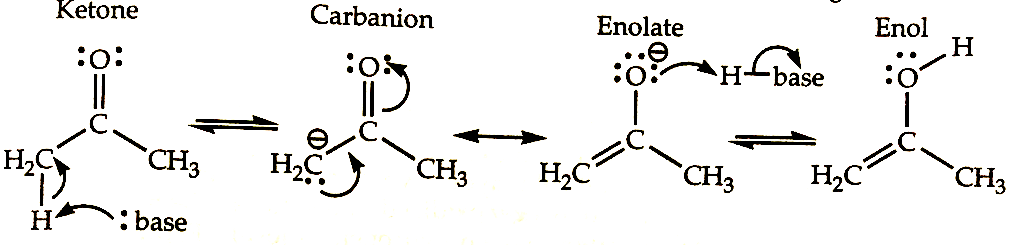
\includegraphics[width=0.65\textwidth]{tautomerization.png} \label{tautomerization}
\caption{Keto-enol tautomerization.}
\end{figure}
\begin{figure}[!ht]
\centering
\includegraphics[width=0.55\textwidth]{longer_ketone.png} \label{longer_ketone}
\caption{Carbanions in ketones to form carbon-carbon bonds.}
\end{figure}
\indent
\indent Oxidizing agents cause oxidation (and in doing so, they get reduced). Oxidizing agents are rich in oxygen, poor in hydrogen, and have an atom in a high oxidation state with high electron affinity. Examples include \ce{KMnO_4}, \ce{RCO_3H}, \ce{O_3}, \ce{NAD+}, \ce{CrO_3}, \ce{ROOR}, \ce{FAD}, and \ce{NADP+}. Reducing agents cause reduction (and in doing so, they get oxidized). Reducing agents are poor in oxygen, rich in hydrogen, and have an atom in a low oxidation state with low ionization energy. Examples include \ce{LiAlH_4}, \ce{HCl}/\ce{Zn}, \ce{H_2}/\ce{Pd}, \ce{NADH}, \ce{NaBH_4}, \ce{H_2NNH_2}/\ce{OH-}, \ce{FADH_2}, and \ce{NADPH}. \\
\indent Oxidation of a primary alcohol with mild oxidizing agent (e.g. PCC in pyridinium) gives an aldehyde. Oxidation of a primary alcohol with strong oxidizing agent (e.g. \ce{K_2CrO_7} followed by acid work up with \ce{H_2SO_4}) gives a carboxylic acid. Oxidation of a secondary alcohol with strong oxidizing agent (e.g. \ce{KMnO_4} followed by base work up with \ce{KOH}) gives a ketone. You can't oxidize a tertiary alcohol because it doesn't have any hydrogen's to lose. For other oxidation reactions, you should simply recognize the oxidizing agent and know that the product is more oxidized than the reactant. The common theme is that one of the reactants (i.e. the oxidizing agent) is rich in oxygen. \\
\indent The two most common reducing agents in carbonyl chemistry are \ce{LiAlH_4} and \ce{NaBH_4}. \ce{LiAlH_4} is more reactive than \ce{NaBH_4}, and so \ce{NaBH_4} reduces only ketones and aldehydes, while \ce{LiAlH_4} reduces all carbonyl compounds. Two important reduction reactions are the aldehyde-to-alkane reactions: \textit{Clemmensen reduction} and \textit{Raney nickel reduction}, respectively. Both can also reduce a ketone to an alkane. These two reactions are shown in \textbf{Fig. \ref{aldehyde-to-alkane}}. Ketones can also be reduced to alkanes using \ce{H_2NNH_2}. 
\begin{figure}[!ht]
\centering
\includegraphics[width=0.55\textwidth]{aldehyde-to-alkane.png} \label{aldehyde-to-alkane}
\caption{Clemmensen reduction (top arrow) and Raney nickel reduction (bottom arrow) for aldehyde reduction into an alkane.}
\end{figure}

\subsection{Name Reactions and Synthesis Logic}
There are specific name reactions that you should know, according to the AAMC's official guide. \\
\indent \textbf{Grignard reactions} involve the addition of a carbanion in the form of a carbanion metal halide to the electrophilic carbon of a carbonyl to form a new carbon-carbon bond. Almost all Grignard reactions generate alcohols. No matter what the reactant, Grignard reactions generate a hydroxyl group in the product where the carbonyl group originated. Keep in mind that if the carbonyl has good leaving groups attached, then it is possible that the Grignard reaction can happen multiple times if there's an excess of the Grignard reagent. Remember that Grignard reagents are strong bases, so it is critical that no protic hydrogens are present. This is why the reaction uses anhydrous ether solvent. The second step in the Grignard reaction (i.e. the work-up step) requires a weak acid, as opposed to a strong acid, to avoid protonation of the hydroxyl group, which can lead to an E\textsubscript{1} elimination reaction. The Grignard reaction can also take place with \ce{CO_2} to form a carboxylic acid. \\
\indent \textbf{Aldol reactions} start with the deprotonation of an $\alpha$ hydrogen from a carbonyl (ketone or aldehyde) using a strong base. The resulting anionic compound (enolate) nucleophilically attacks a neutral carbonyl compound (electrophile) to from a $\beta$ hydroxy carbonyl compound. Under typical reaction conditions, it undergoes elimination to yield and $\alpha, \beta$-unsaturated carbonyl. Regioselectivity is involved, because the final product can have either E or Z structural geometry. The anionic species can also be protonated on the oxygen, resulting in the formation of an enol, but that is in equilibrium with the carbonyl.  The mechanism for aldol condensation is shown in \textbf{Fig. \ref{aldol}}. \\
\begin{figure}[!ht]
\centering
\includegraphics[width=0.55\textwidth]{aldol.png} \label{aldol}
\caption{Aldol condensation mechanism.}
\end{figure}
\indent When the ketone is asymmetric, the choice of which $\alpha$ proton to deprotonate is dictated by reaction. conditions, namely steric hindrance of the transition state and thermodynamic. stability of the intermediates and product. When the major product is selected to minimize steric hindrance in the transition state, this product is said to be the \textit{kinetic product}. This term refers to the lower activation energy required to go through a less sterically hindered transition state. When the major product is selected to maximize stability of the intermediates or product, this product is said to be the \textbf{thermodynamic product}. The reaction has kinetic control at low temperatures with a strong, bulky base, such as t-butOK. The reaction has thermodynamic control at high temperatures with a strong, small base. Aldol reactions have a lot of biological relevance\textemdash for example, the enzyme responsible for the fourth step of glycolysis is an \textit{aldolase}, which catalyzes the retro-aldol reaction. Let's take a look at the following example problem: 
\begin{center}
\begin{minipage}{30em}
\textcolor{blue}{The reaction shown in \textbf{Fig. \ref{6-25}} is best described as:
\begin{enumerate}[label=\Alph*]
	\item a Claisen condensation via the kinetic enolate.
	\item a Claisen condensation via the thermodynamic enolate.
	\item an aldol condensation via the kinetic enolate.
	\item an aldol condensation via the thermodynamic enolate.
\end{enumerate}}
\end{minipage}
\end{center}
\begin{figure}[!ht]
\centering
\includegraphics[width=0.4\textwidth]{6-25.png} \label{6-25}
\caption{Figure for practice problem with aldol condensation.}
\end{figure}
\noindent The reaction involves the condensation of an asymmetric ketone upon itself, which eliminates choices A and B, because the Claisen condensation requires the reaction of esters with esters, not aldehydes or ketones. Because the more hindered $\alpha$ carbon is involved in the addition, the reaction must have been carried out by way of the thermodynamic enolate (more substituted enolate). This makes choice \textbf{D} the best answer.\\
\indent A \textbf{Claisen reaction} is just like the aldol condensation reaction, with the notable exception being that an ester is reacting rather than a ketone or aldehyde. \\
\indent \textbf{Transesterification} involves the exchange of one alkoxy group for another on an ester. Because the equilibrium constant is roughly one, the reaction is driven by either the removal of a product or the addition of a reactant. Transesterification can be carried out in either acid or base. When acid is employed, the mechanism is a typical acid-catalyzed process. In base, the alkoxide nucleophile causes the reactivity. If the base is hydroxide, a carboxylate and alcohol are formed as the two products. The biological applications of transesterification include membrane transport and the conversion of fatty acids into triglycerides. Fatty acids are found in cell membranes; fatty acids that have been esterified with glycerol are broken down in basic water in a process known as \textit{saponification}, generating glycerol and three fatty acid carboxylates.\\
\indent The \textbf{Wittig reaction} converts a carbonyl into an alkene, with stereoselectivity. You can get either the E or Z product depending on what reagents you choose. The Wittig reaction is accomplished by a four-centered intermediate in its last step. See \textbf{Fig. \ref{wittig}} for an example reaction and the associated critical part of the mechanism.
\begin{figure}[!ht]
\centering
\includegraphics[width=\textwidth]{wittig.png} \label{wittig}
\caption{\textit{Left} Example of the Wittig reaction for converting a carbonyl into an alkene with stereoselectivity. \textit{Right} Four-centered intermediate in the last step. The $\varnothing$ symbol is shorthand to represent a phenyl group.}
\end{figure}
\indent The \textbf{Baeyer-Villiger} reaction converts a ketone into an ester using a peroxyacid. The reaction proceeds through an attack of the carbonyl carbon followed by an alkyl migration, which converts a ketone carbon into a more oxidized ester carbon. The \textbf{iodoform reaction} falls in a general class of reactions known as the haloform reactions, which convert a methyl ketone into a carboxylic acid and a haloform, \ce{HCX_3}. The iodoform reaction is used as a chemical test for a methyl ketone, because iodoform is yellow in color and insoluble in water. Methyl ketones react with iodine \ce{I_2} in the presence of strong base to generate a carboxylic acid and deprotonated iodoform molecule. The carboxylic acid is deprotonated to yield a carboxylate and iodoform. Examples of these two reactions are shown in \textbf{Fig. \ref{bv-iodoform}}.\\
\begin{figure}[!ht]
\centering
\includegraphics[width=\textwidth]{bv-iodoform.png} \label{bv-iodoform}
\caption{\textit{Left} Example of the Baeyer-Villiger reaction for converting a ketone into an ester using a peroxyacid. \textit{Right} Example of the iodoform reaction for converting a methyl ketone into a carboxylic acid.}
\end{figure}
\indent The \textbf{W\"olff-Kishner reduction} is a two-step reaction that converts a ketone or aldehyde into an alkane. It is carried out under basic conditions using hydrazine \ce{H_2NNH_2} followed by aqueous hydroxide. The general reaction is shown in \textbf{Fig. \ref{wk}}. Step 1 of the W\"olff-Kishner reaction substitutes a hydrazine for the carbonyl oxygen, resulting in the formation of a hydrozone and water by-product. The first step is reversible with the addition of acidic water, so you can regenerate the carbonyl by adding water and a catalytic amount of acid to the hydrozone. Carbonyls can also react with amines to generate an imine, as we shall see in the nitrogen compound section. Treating the hydrazone with strong base in water generates nitrogen gas and the alkane.\\
\begin{figure}[!ht]
\centering
\includegraphics[width=0.6\textwidth]{wk.png} \label{wk}
\caption{Example of W\"olff-Kishner reaction carried out on cyclopentanone.}
\end{figure}
\indent The steps to analyze a synthetic pathway are:
\begin{enumerate}
	\item Identify the new bonds and functional groups formed by counting the atoms (particularly the carbons) and noting the changes in bonds from reactant to product.
	\item Break the product into fragments that match the reactant skeleton.
	\item Reconnect the fragments with the proper chemical reagents.
\end{enumerate}
\noindent Protecting groups are used when a reactant has multiple reactive sites, but you only wish to react at one of them. Aldehydes are converted into acetals, ketones are converted into ketals, and alcohols are converted into silyl ethers. You must be able to remove the protecting group at the conclusion of the reaction without invoking extreme conditions that may cause the molecule to react. As an example, \textbf{Fig. \ref{alcohol-protection}} shows the conversion of an alcohol into a silyl ether and then back into an alcohol.\\
\begin{figure}[!ht]
\centering
\includegraphics[width=0.55\textwidth]{alcohol-protection.png} \label{alcohol-protection}
\caption{Protection and deprotection of an alcohol.}
\end{figure}
\indent \textbf{Acetoacetic ester} has a carbon that is $\alpha$ to two carbonyl groups. It is referred to as a $\beta$-keto ester, because it has a ketone group on the $\beta$ carbon relative to the ester carbon. ($\beta$-keto esters are formed from a Claisen condensation reaction of two esters).) As a consequence, its protons are more acidic than typical $\alpha$ protons, so it can be deprotonated in mildly basic conditions, resulting in a carbanion. The carbanion is a strong nucleophile, capable of displacing a leaving group to form a new carbon-carbon bond. \textbf{Fig. \ref{acetoacetic-ester}} shows the addition of an alkyl group to acetoacetic ester. Notice that the base of choice matches the alkoxy group of the ester, so that any transesterification reaction that takes place does not result in any change. \\
\begin{figure}[!ht]
\centering
\includegraphics[width=0.55\textwidth]{acetoacetic-ester.png} \label{acetoacetic-ester}
\caption{A typical reaction involving acetoacetic ester.}
\end{figure}
\indent \textbf{Malonic ester}, like acetoacetic ester, has a carbon that is $\alpha$ to two carbonyl groups. As a consequence, the same reactions carried out with acetoacetic ester can also be carried out with malonic ester. However, with malonic ester, a diester is formed, which has two functional groups that can undergo substitution, resulting in cyclization. This is shown in \textbf{Fig. \ref{malonic-ester}}.\\
\begin{figure}[!ht]
\centering
\includegraphics[width=0.55\textwidth]{malonic-ester.png} \label{malonic-ester}
\caption{A typical reaction involving malonic ester.}
\end{figure}
\indent A $\beta$-keto acid (a carboxylic acid with a ketone group on the relative $\beta$ carbon) can undergo \textbf{decarboxylation} when heated. This occurs readily, because the intramolecular hydrogen bonding of a $\beta$-ketoacid aligns the molecule for a shift in the $\pi$-electrons. \textbf{Fig. \ref{decarboxylation}} shows decarboxylation, the six-membered ring created by hydrogen bonding, and the decarboxylation products formed from that conformation. \\
\begin{figure}[!ht]
\centering
\includegraphics[width=0.55\textwidth]{decarboxylation.png} \label{decarboxylation}
\caption{An example of decarboxylation.}
\end{figure}
\indent \textbf{Anabolism} is a reductive process and the result is the build up of a molecule. Examples of anabolism include fatty acid synthesis and gluconeogenesis. \textbf{Catabolism} is an oxidative process and the result is the breakdown of a molecule. Examples of catabolism include glycolysis and $\beta$-oxidation. Typically, catabolism releases energy while anabolism requires, and thereby stores, energy. In humans, oxidations tend to take place in the \textit{mitochondrial matrix} while reductions tend to take place in the \textit{cytoplasm}, with glycolysis being a notable exception. 

\subsection{Carbonyls and Alcohols\textemdash Key Points}
\textbf{Oxygen Containing Compounds}
\begin{enumerate}
	\item Alcohols have higher boiling points than alkanes of roughly equal mass. The boiling points of alcohols are: primary $>$ secondary$>$ tertiary. The hydroxyl group can be converted into a better leaving group\textemdash they are \textit{mesylated} or \textit{tosylated} to form a good leaving group. \ce{SOCl_2} and \ce{PBr_3} convert an alcohol into an alkyl halide.
	\item Aldehydes have strong IR absorbances around 1725 $\text{cm}^{-1}$ and ketones have strong IR absorbanes around 1710 $\text{cm}^{-1}$. They readily form acetals and ketals with alcohol in acid and form hemiacetals and hemiketals with alcohols in base.
	\item Carboxylic acids form more reactive derivatives by converting the hydroxyl group into a better leaving group. \ce{SOCl_2} converts a carboxylic acid into an acyl chloride, heat converts two carboxylic acids into an acid anhydride, and an alsohol in acid converts a carboxylic acid into an ester. Carboxylic acids can be made by complete oxidation of a primary alcohol or aldehyde, or by hydrolysis of acid derivatives such as esters, acid anhydrides, acid halide, amides, and nitriles.
	\item Carboxylic acid derivatives include esters, lactones (cyclic esters), acid anhydrides, acid halides, and amides (where the hydroxyl group of a carboxylic acid is replaced by an amine).
\end{enumerate}
\noindent \textbf{Carbonyl Reactivity}
\begin{enumerate}
	\item Carbonyl compounds are electrophiles that can be attacked at the carbonyl carbon by a nucleophile, forming a tetrahedral intermediate. Strong bases can also deprotonate carbonyl compounds at the $\alpha$-carbon to form a nucleophilic \ce{C}. They can also undergo oxidation-reduction chemistry. Recall that oxidizing agents are rich in \ce{O} and reducing agents are rich in \ce{H}
\end{enumerate}
\noindent \textbf{Name Reactions}
\begin{enumerate}
	\item Grignard reactions add one \ce{R}-group to aldehydes and ketones, forming alcohols, and add twice to carbonyls with a leaving group, forming a tertiary alcohol.
	\item Aldol condensation is the deprotonation of the $\alpha$-carbon of an aldehyde or a ketone and the subsequent addition of the anion to the carbonyl carbon of either a second aldehyde or ketone. It forms an $\alpha, \beta$-unsaturated ketone or an $\alpha, \beta$-unsaturated aldehyde, and can exhibit kinetic versus thermodynamic preference with ketones. The Claisen condensation reaction is similar, but it converts esters into a $\beta$-ketoester.
	\item Transesterification is the conversion of one ester into another by exchanging the alkoxy group, in either acidic or basic conditions.
	\item Wittig reaction is the conversion of a ketone into an alkene via \ce{Ph_3P=CR_2}.
	\item Baeyer-Villiger reaction is the conversion of a ketone into an ester.
	\item Iodoform reaction is the conversion of a methyl ketone into a carboxylic acid.
	\item W\"olff-Kishner reduction is the conversion of a ketone into an alkane in base.
\end{enumerate}
\noindent \textbf{Synthesis}
\begin{enumerate}
	\item The thought process for synthesis involves (1) changes, (2) retrosynthesis, and (3) choosing reagents. Protecting groups are used on reactants with multiple functional groups\textemdash \ce{- OH} group is protected as \ce{- OTMS} and \ce{C=O} group is protected as \ce{C(OR)_2}. 
	\item Acetoacetic ester is a great nucleophile when the $\alpha$-proton is deprotonated, so it readily attacks \ce{C=O}. When treated with acid water and heat, it hydrolyzes and decarboxylates.
	\item Malonic ester readily adds an R-group at the methylene carbon, and can cyclize with a reactant with two nucleophilic sites.
	\item Decarboxylation is observed with $\beta$-keto acids or 1,3 diacids. It proceeds through a six-membered ring held together by an \ce{H}-bond, and forms an enol which equilibrates with the carbonyl compound.
\end{enumerate}
\noindent \textbf{Carbonyl Biochemistry}
\begin{enumerate}
	\item Oxidation and reduction in biochemistry is referred to catabolism and anabolism, respectively. Catabolism occurs mostly in the mitochondrial matrix, while anabolism occurs mostly in the cytoplasm.
	\item Biochemical reagents include \ce{NAD+}/\ce{NADH} (where \ce{NADH} is the reduced form), \ce{FAD}/\ce{FADH_2} (where \ce{FADH_2} is the reduced form), and acetyl coenzyme A (which picks up acetyl groups to form thioester).
\end{enumerate}

\subsection{Monosaccharides}
\textbf{Carbohydrates} are organic compounds with the empirical formula \ce{CH_2O}. Common sugars that you should recognize in all traditional structural representations (Fisher, Haworth, and chair) are glucose, ribose, fructose, galactose, and mannose. Monosaccharides of five carbons or more are typically found in cyclic structures rather than straight chain structures. To form the cyclic structure, a hydroxyl group attacks a carbonyl carbon to form either a hemiacetal (if the sugar is an aldose) or a hemiketal (if the sugar is a ketose). \\
\indent $\alpha$ and $\beta$ glycosidic linkages impact the reactivity and structural nature of polysaccharides. To cleave linkages, specific enzymes are required. Of notoriety is \textit{amylase}, the enzyme that cleaves $\alpha$ linkages in glycogen, amylose, and amylopectin, allowing us to break down starches. Humans lack the enzyme to cleave $\beta$-linkages between glucose residues, so they are unable to breakdown cellulose.\\
\indent \textbf{Monosaccarides} have the basic formula \ce{C_{n}H_{2 n}O_{n}}, with one oxygen attached to every carbon and one unit of saturation, present as either a carbonyl group or a ring. Aldehyde sugars are \textbf{aldoses} and ketone sugars are \textbf{ketoses}. The length of the sugar is also considered in the name\textemdash four carbon sugars are \textit{tetroses}, five carbon sugars are \textit{pentoses}, and six carbon sugars are \textit{hexoses}. \\
\indent A monosaccharide is given D configuration if the hydroxyl group is to the right of the last stereocenter in a Fischer projection, whereas L configuration is given if the OH is to the left of the last stereocenter carbon. The numbering starts on the side nearest the aldehyde or ketone group in linear monosaccharides. Another way of thinking about it is that the last chiral center (found on the penultimate carbon) in the D-isomers of the sugars has R-stereochemistry, while the last chiral center in the L-isomers of the sugars has S-stereochemistry. Note that there exists no correlation between D and L with (+) and (-) optical rotation. We are enzymatically programmed to digest D-sugars as opposed to L-sugars. As an example, take a look at the 4 stereoisomers of aldotetrose, shown in \textbf{Fig. \ref{aldotetrose}}. \\
\begin{figure}[!ht]
\centering
\includegraphics[width=0.6\textwidth]{aldotetrose.png} \label{aldotetrose}
\caption{Fischer projections for each of the four stereoisomers of aldotetrose.}
\end{figure}
\indent Sugars are routinely represented by \textbf{Fischer projections}, which are short hand for the top view (top perspective) of a compound in its fully eclipsed conformation. The Fischer projection is derived from the straight chain form\textemdash any substituent on the right or left side of the main backbone is projecting out at you. The translation into a Fischer projection from a three dimensional structure is shown in \textbf{Fig. \ref{fischer}}.\\
\begin{figure}[!ht]
\centering
\includegraphics[width=0.55\textwidth]{fischer.png} \label{fischer}
\caption{Example of translating a traditional chemical structure into a Fischer projection.}
\end{figure}
\indent Most sugars encountered in biology are pentoses and hexoses, as opposed to tetroses. Recall from stereochemistry that an \textbf{epimer} is one of a pair of stereoisomers that differ in the absolute configuration of a single stereocenter. When the molecule has only one stereocenter then the epimers are \textit{enantiomers}. When the molecule has two or more stereocenters then the epimers are \textit{diastereomers}. \textbf{Anomers} are cyclic monosaccharides or glycosides that are epimers, differing from each other in the configuration of C-1 if they are aldoses or in the configuration at C-2 if they are ketoses. The most important differences between them is this:
\begin{equation}
\begin{split}
\boxed{\text{Anomers vary in chirality at the most oxidized carbon. Epimers vary in chirality at a less oxidized, backbone carbon.}}
\end{split}
\end{equation}
\noindent The anomeric carbon is the former carbonyl carbon in a sugar. The most stable form of sugar is the cyclic form, which forms when a hydroxyl group attacks the carbonyl carbon to yield a hemiacetal. This generates a new chiral center at the anomeric carbon. Because the attack can occur from either top or bottom, there are two diasteromers formed. The two diasteromers are referred to as anomers and the new chiral carbon is the anomeric carbon. The two anomers are reffered to as the $\alpha$ (axial for D-pyranoses) and $\beta$ (equatorial for D-pyranoses) anomers. The $\beta$ anomer is typically more stable than the $\alpha$ anomer. It is only in the cyclic form (\textit{furanose form} for five-membered rings and \textit{pyranose form} for six-membered rings) that anomers are possible. This is because six-membered rings are referred to as \textbf{pyrans} while five-membered rings are referred to as \textbf{furans}. An example of anomers is shown in \textbf{Fig. \ref{anomers2}}. \\
\begin{figure}[!ht]
\centering
\includegraphics[width=0.55\textwidth]{anomers2.png} \label{anomers2}
\caption{An example of anomers with $\alpha$- and $\beta$- D-glucopyranose.}
\end{figure}
\indent The best way to memorize the $\alpha$ vs. $\beta$ distinction is that \textbf{in cyclic sugar structures, the term $\alpha$ technically means that the anomeric oxygen is trans with respect to the last carbon (C-6 for D-glucopyranose), and the term $\beta$ technically means that the anomeric oxygen is cis with respect to the last carbon.} The two anomers of a sugar exist in equilibrium \textbf{in vivo} and can interchange via a straight chain intermediate. Conversion from one anomer into the other is known as \textbf{mutarotation}. \\
\indent Memorizing the names and structures for all sugars is no doubt a little pointless, but knowing the common monosaccharides is not a bad idea. Common monosaccharides in biochemistry include ribose, glucose, mannose, fructose, and galactose. To help recall common sugars, we shall present a mnemonic for three of them:
\begin{enumerate}
	\item To help recall glucose, we have a not-so-nice way to remember the position of the hydroxyl groups. Using your right hand, if you `flip off' the page with the fingernail of your middle finger facting the page, then you fingertips are positioned just as the hydroxyl groups of D-glucose are positioned in its Fischer projection. This helps with enantiomers too\textemdash D-glucose is found using your right hand while L-glucose is found using your left hand.
	\item Mannose can be recognized by making a gun figurine using your middle and index fingers as the barrel (a `double-barrel' gun)\textemdash your fingertips then mimic the positions of the hydroxyl groups in the Fischer projection of D-mannose. Statistically speaking, a man is more likely to have a fun than a woman, so mannose is based on a man gun hand. 
	\item D-Ribose has all of its hydroxyl groups on the right side of its Fischer projection, so `ribose is all right!'
	\item Fructose is the ketose of glucose and galactose is the C-4 epimer of glucose.
\end{enumerate}
\noindent These suggested mnemonics are shown in \textbf{Fig. \ref{fuck_glucose}}.\\
\begin{figure}[!ht]
\centering
\includegraphics[width=0.55\textwidth]{fuck_glucose.png} \label{fuck_glucose}
\caption{Mnemonic devices for memorizing the common monosaccharides.}
\end{figure}
\indent The \textbf{Haworth projection} is a simplified representation of cyclic sugars. They have no physical relevance, but are easy to draw\textemdash they do not show the three-dimensional spacing that chair conformations show, but they emphasize positions above and below the ring, which is the major focus with sugars. Converting from the Fischer projection to the Haworth projection is easy once you get the hang of it. To go from straight chain to the ring form, recall the phrase `\textbf{\textit{downright uplefting}},' which applies to carbons 2, 3, 4 in an aldohexose, but not the penultimate carbon (which has its oxygen in the ring) or the anomeric carbon. Any hydroxyl groups on the right side in the Fischer projuection end up below the ring in its cyclic structure, and any hydroxyl groups on the left in the Fischer projection end up above the ring in its cyclic structure. Numbering the carbons makes it easier to convert to the Haworth projection, because it helps to keep track of carbons 2, 3, and 4. The anomeric carbon is given the far right position in the Haworth projection. \textbf{Fig. \ref{haworth}} shows the generation of the Haworth projection of D-galactopyranose. An important skill to have is the ability to recognize sugars relative to glucose and to be able to quickly convert from the ring structure to the straight chain structure, as these are the common ways in which you will see sugars.\\
\begin{figure}[!ht]
\centering
\includegraphics[width=0.55\textwidth]{haworth.png} \label{haworth}
\caption{Generating the Haworth projection of D-galactopyranose.}
\end{figure}
\indent In addition to doing mutarotation, monosaccharides can conver from an aldose into a ketose via an \textit{enediol intermediate} in a conversion known as \textit{ketose-aldose isomerization}. In glycolysis, the enzyme \textit{isomerase} converts glucose-6-phosphate into fructose-6-phosphate via this process. Also in glycolysis, an isomerization process similar to tautomerization converts dihydroxyacetone phosphate into glyceraldehyde-3-phosphate. \textbf{Fig. \ref{kai}} shows the step-by-step conversion of an aldose into a ketose in both acid and base.\\
\begin{figure}[!ht]
\centering
\includegraphics[width=0.55\textwidth]{kai.png} \label{kai}
\caption{Mechanism of ketose-aldose isomerization. The bolded hydrogen atoms are the active hydrogens that are being either gained or lost in the reaction mechanism. The requirement for the conversion is the formation of either the enol (under acidic conditions) where the carbonyl oxygen is protonated and the $\alpha$ hydrogen is deprotonated, or the formation of the enolate (under basic conditions) where the $\alpha$ hydrogen is deprotonated.}
\end{figure}

\subsection{Oligosaccharides and Polysaccharides}
Sugars combine when a \ce{-OH} group of one sugar attaches the hemiacetal carbon of a second sugar, displacing the hydroxyl group from the hemiacetal carbon to form an acetal. This forms a \textbf{\textit{glycosidic linkage}}, resulting from a dehydration reaction of the two hydroxyls involved. The terms used to describe the orientation of the anomeric hydroxyl group in a cyclic monosaccharide (i.e. $\alpha$ and $\beta$) are also used to describe the orientation of the oxygen in the glycosidic linkage\textemdash when the anomeric oxygen is cis with respect to the last carbon (i.e. C-6 in an alcohexapyranose), the linkage is said to be $\beta$. The names for disaccharides are derived from the two component sugars where the left sugar (using hydroxyl 1 of an aldopyranose) is considered a substituent on the right sugar (using either hydroxyl 4 or 6(. The left sugar get an `-osyl' suffix and the right sugar gets an `-oside' suffix. For instance, lactose consists of galactopyranosyl and glucopyranoside. In most cases, the linkage is 1,4, as in the disaccharides maltose, cellobiose (formed from the hydrolysis of cellulose) and lactose. In sucrose, the linkage is 1,2, which is rare. \textbf{Fig. \ref{disaccharides}} shows the structures and nomenclature of these common disaccharides.\\
\begin{figure}[!ht]
\centering
\includegraphics[width=0.55\textwidth]{disaccharides.png} \label{disaccharides}
\caption{Common disaccharides and their structures.}
\end{figure}
\indent We store sugars in polymers such as \textit{glycogen}, which has 1,4-$\alpha$ linkages between adjacent glucopyranoses and 1,6-branching about one out of every ten glucopyranose residues. Amylopectin and glycogen have branching, while amylose does not. The most abundant of all polysaccharides is cellulose (poly $\beta$-D-glucopyranose), which is used for structural purposes in plants. There are no 1,6-linkages found in cellulose, only 1,4-linkages. This means that cellulose is a linear polymer with no branching. 

\subsection{Chemical Reactions and Tests for Carbohydrates}
\indent \large\textbf{Nitric Acid Sugar Oxidation:} \normalsize Nitric acid is rich in oxygen, making it an oxidizing agent. When an aldohexose is treated with nitric acid, both terminal carbons are oxidized into carboxylic acid groups. If the product, called an \textit{aldaric acid}, is meso, then the compound is optically inactive. Using retro-analysis, the chirality of the hydroxyl groups in the original monosaccharide can be determined. \textbf{Fig. \ref{no3_oxidation}} shows the aldaric acid formation reactions of four aldohexoses.\\
\begin{figure}[!ht]
\centering
\includegraphics[width=0.55\textwidth]{no3_oxidation.png} \label{no3_oxidation}
\caption{Nitric acid sugar oxidation test.}
\end{figure}
\indent \large\textbf{Osazone Test:} \normalsize Really, the osazone test should be more aptly named the \textit{epimer test}. When treated with three equivalents of phenyl hydrazine (\ce{HPhNNH_2}), an aldose or 2-ketose undergoes a substitution reaction to form an imine, followed by the oxidation of an alcohol into a carbonyl, and lastly a second substitution reaction forming a second imine group. Imine moieties form at carbons 1 and 2, so any chirality at either carbon is lost. As a consequence, C-2 epimers yield the same osazone. \textbf{Fig. \ref{osazone}} shows that D-mannose, D-fructose, and D-glucose all yield the same osazone. The osazone test works in conjunction with other information to zero in ont he identity of an unknown sugar.\\
\begin{figure}[!ht]
\centering
\includegraphics[width=0.55\textwidth]{osazone.png} \label{osazone}
\caption{Example of the osazone test with C-2 epimers.}
\end{figure}
\indent \large\textbf{Tollen's Test:} \normalsize The Tollen's test involves the reduction of \ce{Ag+} by an oxidizable sugar. As silver ion is reduced to silver metal, if the solution is spun within the container, then silver precipitates on the inside walls, resulting in a `silver mirror.' The Tollen's test is said to be positive if the silver mirror forms rapidly, indicating the presence of an aldose.\\
\indent \large\textbf{Kiliani-Fischer Synthesis:} \normalsize The Kiliani-Fischer synthesis increases the carbon chain of an aldose by one. Note that it doesn't work with ketoses. The new carbon is added as a cyano group to the carbonyl carbon, so the chain increases by one carbon at the aldehyde end. After reduction to an imine and hydrolysis, the cyano group is converted into an aldehyde. The result is the formation of \textit{two} aldose epimers with an additional carbon. As an example \textbf{Fig. \ref{kfs}} shows the Kiliani-Fischer synthesis of two D-aldohexoses from D-arabinose. An \ce{-OH} group in parenthesis represents the possibility of both chiral centers.\\
\begin{figure}[!ht]
\centering
\includegraphics[width=0.55\textwidth]{kfs.png} \label{kfs}
\caption{Kiliani-Fischer synthesis of two D-aldohexoses from D-arabinose.}
\end{figure}
\indent \large\textbf{Ruff Degradation:} \normalsize In Ruff degradation, an aldose loses its first carbon, resulting in an aldose of one less carbon. As we saw in the carbonyl section and in several biochemistry examples, losing one carbon is readily accomplished by decarboxylation. In order to decarboxylate the terminal carbon, it must be oxidized first to a carboxylic acid and then to carbon dioxide. Bromine in water effectively converts the aldehyde into a carboxylic acid (or in the ring form, a hemiacetal into a lactone). The carboxylic acid is oxidized into \ce{CO_2} by peroxide in the presence of a ferric cation catalyst. \ce{CO_2} leaves and decreases the chain length by one carbon. \textbf{Fig. \ref{ruff}} shows the Ruff degradation of D-glucose. It is rarely used with aldopentoses, because when the product is an aldotetrose, the yield is low, likely due to the difficulty encountered with a smaller ring in the cyclic form. 
\begin{figure}[!ht]
\centering
\includegraphics[width=0.55\textwidth]{ruff.png} \label{ruff}
\caption{Ruff degradation of D-glucose into D-arabinose.}
\end{figure}

\subsection{Biological Examples of Carbohydrates}
As a general rule, natural sugars have D-chirality. This is because our enzymes recognize D-sugars, and therefore select for D-sugars. One notable exception to the `D only' rule includes the presence of L-fucose, a reduced from of L-galactose, in the glycoproteins of blood type markers. \\
\indent Carbohydrates are also important for \textbf{glycolysis}. Before we get into this, note that \textbf{you should \textit{not} memorize glycolysis}, as the amount of time invested to do so would not have a good return in terms of increasing your MCAT performance. However, you \textit{should} have a basic idea of what happens overall. You should know that glucose is converted into pyruvate and that there is a net generation of 2 ATP and a release of energy.\\
\indent Glycolysis is a ten-step metabolic process. During the process, two net equivalents of ATP are formed, and also two equivalents of the oxidizing agent \ce{NAD+} are also required. The basic steps are as follows:
\begin{enumerate}
	\item Conversion of glucose into glucose-6-phosphate, basically tagging on a phosphate group to C-6. This is the first committed step in glycolysis, and releases a great deal of energy.
	\item Step II involves isomerization of the aldose, and step III adds another phosphate group. Not super interesting.
	\item In step IV, a six-carbon molecule is cleaved into 2 three-carbon molecules by a \textit{reverse Aldol reaction} that breaks the bond between C-3 and C-4 of fructose-1,6-diphosphate (a $\beta$-hydroxyketone), forming dihydroxyacetone phosphate (DHAP) and glyceraldehyde-3-phosphate (G-3-P). 
	\item Step V converts DHAP into G-3-P by way of an isomerization reaction. As of step V, no oxidation has occurred.
	\item Step VI oxidizes the aldehyde G-3-P into 1,3-bisphosphoglyerate (a carboxylic acid derivative). It is the \textit{only} oxidation step in glycolysis. 
	\item Step VII dephosphorylates 1,3-bisphosphoglyerate into 3-phosphoglycerate, releasing a phosphate for the regeneration of ATP that was invested in earlier steps. Step VIII converts 3-phosphoglycerate into 2-phosphoglycerate. This is to position the phosphate for enol formation in the next step.
	\item Step IX is enolate formation. Phosphoenolpyruvate is formed from 2-phosphoglycerate, and involves \textbf{dehydration}.
	\item Step X finishes the process, converting phosphoenolpyruvate into pyruvate using the enzyme \textit{pyruvate kinase}.
\end{enumerate}
\noindent One pyruvate is formed, it can undergo either aerobic or anaerobic breakdown. Pyruvate can undergo fermentation, where C-2 is reduced from a ketone into an alcohol, resulting in the formation of lactate, which regenerates \ce{NAD+}. We can't reduce lactate any further (only yeast and bacteria can convert pyruvate into \ce{EtOH}), so it is excreted as waste. Pyruvate can also undergo oxidative decarboxylation yielding \ce{CO_2} and Acetyl-CoA\textemdash this sets up the cell for performing downstream aerobic respiration. 

\subsection{Common Nitrogen Compounds}
Unlike the drastic difference in reactivity between an ether and an alcohol, amines do \textit{not} change their reactivity significantly as they become more substituted. Steric hindrance and electron density on the nitrogen are impacted by substitution, but not to the degree that tertiary amines are significantly more or less reactive than primary amines. Of significance when considering amines are their basicity and their nucleophilicity. This makes up the bulk of their reactions.\\
\indent \textbf{Amines} are compounds with a central nitrogen that has three $\sigma$ bonds to either \ce{C} or \ce{H}. The degree of substitution of the amine is described as \textit{primary} (one substituent), \textit{secondary} (two substituents), or \textit{tertiary} (fully substituted with three substituents). If the nitrogen has a double bond to carbon, the compound is known as an \textbf{imine}. If a hydrogen on the amine nitrogen is replaced by an \ce{-OH} group, the compound is known as a \textbf{hydroxyamine}. Nitrogen when bonded to nitrogen by a $\sigma$ bond is a \textbf{hydrazine}.\\
\indent Amines are both weak bases and good nucleophiles. They are found in many neurobiology compounds because many amines have stimulating effects on the brain. Some examples include morphine, nicotine, cocaine, amphetamine, epinephrine, and mescaline. \\
\indent Because the nitrogen of the amine has a long pair of electrons, nitrogen atoms can serve as a nucleophilic or basic center for a molecule. Amines are kind of complicated, as the impact of steric hindrance, hydrogen bonding in solution, and electronics is not as predictable as it is with most other compounds.  In general, amines are often used as weak bases\textemdash the varying basicity of amines can be attributed to factors such as the inductive effect, steric hindrance, hydrogen bonding, and solvation. The seemingly chaotic order of relative amine basicity demonstrates the presence of both the inductive effect and steric factors. More specifically, steric factors would favor a smaller base, because of its ability to bind a proton with little to no hindrance. The inductive effect predicts that the more substituted amine is the most basic. The relative basicity of the methyl amines is \ce{(H_3C)_2NH}$>$\ce{H_3CNH_2}$>$\ce{(H_3C)_3N}$>$\ce{NH_3}. As an example, consider the reaction \ce{H_3CNH_2 + NH_4+ <=> H_3NH_3+ + NH_3}. Because the methyl group is \textit{electron donating}, methylamine is more basic than ammonia. This means that the ammonium cation is more acidic than the methyl ammonium cation. Here is an example problem:
\begin{center}
\begin{minipage}{30em}
\textcolor{blue}{Given that the pK\textsubscript{b} of \ce{NH_3} is 4.74, what is the approximate pK\textsubscript{b} of \ce{Et_3N}?
\begin{enumerate}[label=\Alph*]
	\item -0.32
	\item 3.25
	\item 5.31
	\item 9.26
\end{enumerate}}
\end{minipage}
\end{center}
\noindent Alkyl groups are electron donating, so triethyl amine \ce{Et_3N} is more basic than ammonia. As a consequence, the pK\textsubscript{b} for triethyl amine must be less than 4.74, eliminating choices C and D. A negative pK\textsubscript{b} corresponds to a strong base and amines are weak bases, so choice A is too low. Therefore, choice \textbf{B} is the best answer.\\
\indent Weak bases, such as amines, make good nucleophiles and the nucleophilicity of amines parallels their basicity for the most part. Deviations from this trend are due to steric hindrance. The majority of amine reactions in organic chemistry involve the amine behaving as a nucleophile by attacking an electrophile and either replacing a leaving group or breaking a $\pi$ bond.\\
\begin{center}
\begin{minipage}{30em}
\textcolor{blue}{What is the major organic product when ammonia, \ce{NH_3}, is treated with excess ethyl iodide \ce{H_3CCH_2I} following workup?
\begin{enumerate}[label=\Alph*]
	\item \ce{H_2C=CH_2}
	\item \ce{H_3CCH_2NH_2}
	\item \ce{(H_3CCH_2)_2NH}
	\item \ce{(H_3CCH_2)_3N}
\end{enumerate}}
\end{minipage}
\end{center}
\noindent Because secondary amines are better nucleophiles than primary amines, which in turn are better nucleophiles than ammonia, the reaction proceeds until the alkyl halide is exhausted. With excess alkyl iodide, the reaction is free to add as many ethyl groups to the amine as possible. The best choice shows three alkyl groups added to the amine. This makes the correct answer choice \textbf{D}. It is possible that \ce{(H_3CCH_2)_4N+}, a quaternary amine, would form, but it is not listed as an answer choice.\\
\indent When amines are added to a carbonyl, a nucleophilic attack at the carbonyl carbon takes place. If there is no leaving group on the carbonyl, then the reaction forms an \textbf{imine} and water, and is driven by its equilibrium. An \textbf{imine} is a carbon double bonded to a nitrogen (\ce{C=N}). This reaction proceeds considerable better with an aldehyde than a ketone, attributed primarily to the greater electrophilicity of an aldehyde than a ketone. The basic idea here is that by saturating an aldehyde or ketone with a compound that contains at least two hydrogen atoms on the nitrogen, a \ce{C=O} bond is converted into \ce{C=N}. With excess water, the reverse reaction is observed. \\
\indent Just as ketones and aldehydes undergo tautomerization in the presence of mild acid or mild base to form an enol, imines also undergo \textbf{imine-enamine tautomerization} to form an \textit{enamine}. \textbf{Fig. \ref{iet}} shows the equilibrium between an imine and an enamine. An imine can form from the reaction of an amine and a carbonyl group only if the nitrogen compound has two hydrogen atoms on the nitrogen (otherwise there's no way to form the water product). The formation of an enamine from a secondary amine and ketone is shown in \textbf{Fig. \ref{enamine}}. \\
\begin{figure}[!ht]
\centering
\includegraphics[width=0.55\textwidth]{iet.png} \label{iet}
\caption{Mechanism of imide-enamine tautomerization.}
\end{figure}
\begin{figure}[!ht]
\centering
\includegraphics[width=0.55\textwidth]{enamine.png} \label{enamine}
\caption{Formation of an enamine from a secondary amine and ketone.}
\end{figure}
\indent \textbf{Amides} are carbonyl compounds with a nitrogen bonded to the carbonyl carbon. The are formed when an amine or ammonia is added to a carbonyl compound with a leaving group. In primary amides, the nitrogen is bonded to two hydrogens; in secondary amides, the nitrogen is bonded to one hydrogen; in tertiary amides, the nitrogen is bonded to no hydrogens. When an amide is part of a cyclic structure, then the compound is referred to as a \textbf{lactam}. Lactams are classified by the position of the carbon bonded to nitrogen relative to the carbonyl group of the amide. For instance, a $\beta$-lactam is a four membered lactam ring containing two $sp^3$-hybridized carbons, a carbonyl carbon, and the amide nitrogen. \textbf{Fig. \ref{lactams}} shows a $\beta$-lactam (a class of antibiotic), a $\gamma$-lactam, and a $\delta$-lactam.\\
\begin{figure}[!ht]
\centering
\includegraphics[width=0.65\textwidth]{lactams.png} \label{lactams}
\caption{Examples of different types of lactams.}
\end{figure}
\indent In an aqueous environment at neutral pH, the carboxyl terminal is deprotonated and the amino terminal is protonated in an amino acid, so it has at least two charged sites despite having no net charge\textemdash this is referred to as a \textbf{zwitterion}. However, in organic solvents and lipid environments they exist as an uncharged molecule. There are two synthetic pathways for making amino acids: the \textbf{Gabriel synthesis} and the \textbf{Strecker synthesis}. The Gabriel method involves reacting a phthalimide with malonic ester, followed by the addition of the R-group (side chain) and acid-catalyzed decarboxylation. The Strecker synthesis method involves with an aldehyde that contains the R-group of the desired amino acid, and the subsequent conversion into an imine, addition of a cyano group, and finally hydrolysis of the \ce{C#N} triple bond using acidic water. Both of these syntheses are shown in \textbf{Fig. \ref{aasynthesis}}.\\
\begin{figure}[!ht]
\centering
\includegraphics[width=0.7\textwidth]{aasynthesis.png} \label{aasynthesis}
\caption{The Gabriel synthesis and Strecker synthesis of amino acids.}
\end{figure}

\subsection{Amino Acids and Proteins}
Amino acids are essentially just polyprotic acids where all of the protons are weakly acidic. The amino terminal, when protonated, forms a cation with a pK\textsubscript{a} of roughly $9.7\pm0.9$, and the carboxylic acid terminal has a pK\textsubscript{a} of roughly $2.2\pm0.4$ (these numbers are important, make sure to memorize them!). Amino acids also have a chiral center at the $\alpha$-carbon in all amino acids except glycine. Naturally occurring amino acids have \textit{S-stereochemistry} at C-2, although in biochemistry we refer to that as the L-amino acid. The only exception to this pseudo-rule where L corresponds to S is cysteine, where L-cysteine is the natural form, but it has R stereochemistry at the $\alpha$-carbon. All of the amino acids and their structures/abbreviations are shown in \textbf{Fig. \ref{Amino_Acids}}\textemdash \textit{make sure to memorize it}! \\
\indent The hydrophobic amino acids are Phenylalanine (Phe, F), Leucine (Leu, L), Alanine (Ala, A), Isoleucine (Ile, I), and Valine (Val, V). In aqueous environments, hydrophobic amino acids are found in the core of a folded protein. \textit{Semi-hydrophobic amino acids} are typically considered to be hydrophobic in most text books, but we segregate them from other hydrophobic amino acids because they don't pack as well as the alkyl side chains. These include the side chains with a nitrogen in a ring (i.e. Tryptophan (Trp, W), Proline (Pro, P)), a sulfur-containing Methionine (Met, M), and Glycine (Gly, G). Hydrophilic amino acids prefer to be situated in an aqueous environment\textemdash in water, hydrophilic amino acids are found on the exterior of a folded protein. These are sometimes referred to as \textit{protic} side chains. Hydrophilic amino acids include Serine (Ser, S), Threonine (Thr, T), Cysteine (Cys, C), Tyrosine (Tyr, Y), Glutamine (Gln, Q), and Asparagine (Asn, N). A good mnemonic for recalling the six hydrophilic amino acids that don't fall into the acidic or basic category is \textbf{``See There, my CysTyr does not have a Glue Ass''} for remembering them in the order shown above. \\
\indent Acidic amino acids have side chains that lose a proton from their neutral state. They have three acidic sites\textemdash the N-terminal, the C-terminal, and the side chain. In the case of Glutamic acid (Glu, E) and Aspartic acid (Asp, D), the side chain is a carboxylic acid, and so they are the two acidic amino acids. Cysteine and tyrosine can technically also lose a proton from their neutral side chain, but it happens at a high enough pH that we generally think of them as polar rather than as acidic. Basic amino acids have side chains that gain a proton from their neutral state. The three basic amino acids are Lysine (Lys, K), Arginine (Arg, R), and Histidine (His, H), and all have nitrogen-containing side chains. Like acidic amino acids, basic amino acids have their associated R-group pK\textsubscript{a} values. A useful mnemonic is \textbf{``his lies are basic,''} which means that histidine, lysine, and arginine are basic. For histidine, the lower nitrogen in the imidazole ring is its basic site. \textbf{Fig. \ref{abaa}} shows the charged amino acids in an aqueous environment at pH=7.\\
\begin{figure}[!ht]
\centering
\includegraphics[width=0.8\textwidth]{abaa.png} \label{abaa}
\caption{pK\textsubscript{a} values and structures of charged amino acids in an aqueous environment at pH=7.}
\end{figure}
\indent There are some fundamental structural features of proteins that result from properties of their component amino acids. Cross-linking of cysteine residues is one example. Another structural feature is \textit{structural turns}, forced alterations in the structure of a protein, caused by proline. Proline is cyclic and thus unable to rotate freely about its $\sigma$ bonds. It is locked into a cyclic conformation, which locks the protein backbone into a turn. \\
\indent In aqueous solution at a pH of 7, an amino acid exists as an ionic species\textemdash the amino terminal is protonated and the carboxyl terminal is deprotonated. The net result is zero overall charge for hydrophobic amino acids, and the structure is referred to as a \textit{zwitterion}. The pH at which the zwitterion exists in highest concentration is referred to as the \textbf{isoelectric pH}. The isoelectric pH is obtained by averaging the two pK\textsubscript{a} values that involve the neutral molecule. The isoelectric point coincides with an equivalence point on a titration curve, the first equivalence point of all amino acids except the ones with basic side chains, where it coincides with the second equivalence point. To calculate the isoelectric pH, you must first decide if the side chain is acidic, basic, or neutral. For amino acids with neutral or acidic side chains, the isoelectric point is found by averaging pK\textsubscript{a1} and pK\textsubscript{a2}. For amino acids with basic side chains, the isoelectric point is found by averaging pK\textsubscript{a2} and pK\textsubscript{a3}. \\
\indent What if we want to get the isoelectric point pI of an entire protein? The pI for a protein is found by summing the number of basic amino acids plus one, and taking the pK\textsubscript{a} with that numerical subscript and averaging it with the next pK\textsubscript{a} value sequentially up. As an example, consider the short polypeptide chain shown in \textbf{Fig. \ref{isoelectric_example}}. This sample protein has a lysine and histidine, so the pI is an average of pK\textsubscript{a3} and pK\textsubscript{a4}. The final step would be to determine which pK\textsubscript{a} values are which. For this protein of interest, pK\textsubscript{a1} is for the carboxyl terminal (this is true for \textit{any} protein). The sequence of the remaining pK\textsubscript{a}'s must be determined from numerical pK\textsubscript{a} values.\\
\begin{figure}[!ht]
\centering
\includegraphics[width=0.7\textwidth]{isoelectric_example.png} \label{isoelectric_example}
\caption{Example problem on how to determine the isoelectric point of a protein.}
\end{figure}
\indent The assignment of pK\textsubscript{a} values is sequential with increasing numerical value, so the pI for this protein is found by averaging pK\textsubscript{a3}=4.3 and pK\textsubscript{a4}=6.1, which results in a pI of 5.2. This means that at pH=5.2, the protein exists as a zwitterion, at pH<5.2 it exists as a cation, and at pH>5,2 it exists as an anion. Here is another example problem:\\
\begin{center}
\begin{minipage}{30em}
\textcolor{blue}{What is the isoelectric point for tyrosine?
\begin{enumerate}[label=\Alph*]
	\item 2.2
	\item 5.6
	\item 6.2
	\item 9.1
\end{enumerate}}
\end{minipage}
\end{center}
\noindent The isoelectric point is found by averaging pK\textsubscript{a1} and pK\textsubscript{a2} for all amino acids except Lys, Arg, and His. The isoelectric point for tyrosine is found using
\begin{equation}
\begin{split}
pI=\frac{\ce{pK_{a1}}+\ce{pK_{a2}}}{2}=\frac{2.2+9.1}{2}=\frac{11.3}{2}\approx5.6
\end{split}
\end{equation}
\noindent Therefore, choice \textbf{B} is the best answer. As a general rule, acidic amino acids have pI values \textit{less than} 5.5, and basic amino acids have pI values \textit{greater than} 7.5. All other amino acids have a pI value within the 5.5 to 7.5 range.\\
\indent There are two types of gel electrophoresis lab techniques that you should know about. The first type of electrophoresis employs a pH gradient in the gel and the charged species igrate through the gel until they reach a pH equal to their pI. At that point, they have no net charge, so there is no electric force. This technique is referred to as \textbf{isoelectric focusing}. The second type of electrophoresis involves adding \textit{sodium dodecyl sulfate}, SDS, to the protein mixture. The protein fragments incorporate SDS into their secondary structure, resulting in every fragment taking on a negative charge. Larger protein fragments can incorporate more SDS than smaller ones, resulting in a greater magnitude of charge. However, larger species are more massive. As a result, the incorporation of SDS creates an environment where all of the protein fragments have the same mass-to-charge ratio. Given that they are experiencing the same electric field, separation is due to size differences, where small species migrate faster than larger species.\\
\indent Another technique that can separate proteins according to their charge is \textbf{affinity chromatography}. We will look specifically at \textbf{ion-exchange chromatography}, which separates by the affinity of charged proteins for oppositely charged sites on the polymer in the column (stationary phase). The stationary phase is made of an insoluble polymer, often polystyrene or cellulose, to which functional groups capable of carrying a charge have been attached. Positively charged columns bind anionic species and negatively charged columns bind cationic species. A protein carries a positive charge when the solution pH is less than the isoelectric point of the protein. When a mixture of proteins is added to the column and allowed to migrate down the polymer, selected proteins can be separated from the mixture when they bind the column, while proteins carrying the same charge as the column elute. To release a bound protein from an ion-exchange column, the polymer can be washed with a solution of varying pH or a solution of gradually increasing salt concentration. Note that both techniques for releasing the protein could denature it irreversibly, so the preferred technique is not always obvious.\\
\indent There's also \textbf{size-exclusion chromatography} (also known as \textit{gel-filtration chromatography}) to separate proteins. A standard column is filled with agarose beads or dextran, which have natural pores of varying size. As the mixture migrates down the column, smaller species get caught within the pores, which slows down their progress, while larger proteins get caught in fewer pores, so they traverse the column in less time.\\
\indent Determining the primary sequence of a protein is important, but automated sequencing has upper limits as to the number of amino acids that can be sequentially identified, so it is best to break a large protein into smaller, more manageable fragments. Each fragment can be sequenced and then the fragments can be reassembled to determine the overall sequence of the original protein. \\
\indent The original protein must be marked such that the first and last fragments are easy to identify. The first amino acid in the sequence can be identified by adding 2,4-dinitrofluorobenzene (\textbf{Sanger's reagent}) to the protein, followed by complete hydrolysis using \ce{HCl}. Sanger's reagent binds to the N-terminus of a protein, thereby labeling the first amino acid. The protein is then broken down into smaller fragments, often using chemicals/enzymes that are derived from nature.\\
\indent Sequencing is often done in multiple steps. Prior to sequencing, a protein is typically treated with urea and $\beta$-mercaptoethanol. Urea denatures the protein by breaking the H-bonds holding it together, and $\beta$-mercaptoethanol breaks cross-linking. Once the protein's secondary and tertiary sequence is denatured, its primary structure can be sequenced.\\
\indent To sequence the amino acids in a small polypeptide (20 to 50 amino acids typically), biochemists employ \textbf{Edman's reagent}, phenylisothiocyanate (\ce{H_5C_6N=C=S}). This reagent sequentially removes each amino acid one at a time starting from the amino terminal. This leads to the automated sequencing equipment used in most biology labs. \\
\indent A common rule in the chemistry of amino acids is that they exist exclusively as L-stereoisomers in biological systems. An exception to this ``all amino acids are L'' rule is found in the bacterial cell wall. The cell wall of a bacteria is held together by a net-like structure that involves a cross-link between D-alanine and glycine. As a point of biological interest, $\beta$-lactams such as penicillin act in a medicinal fashion by breaking this linkage and destroying the cell walls of bacteria.

\section{Physics}
\subsection{Translational Motion}
In general on the MCAT, although especially for the physics section, it's about speed more than precision. Important kinematic equations that you probably don't know yet:
\begin{equation}
\begin{split}
\Delta x = \frac{1}{2}\left(v_0+v_f\right)\Delta t, \quad v_f^2=v_0^2+2a\Delta x
\end{split}
\end{equation}

\subsection{Forces and Torque}
\indent In order to handle formula identification problems \textit{quickly} (as speed is extremely important on the exam), the two best techniques are \textbf{checking units} and considering \textbf{limiting cases}. For example, consider the following problem:
\begin{center}
\begin{minipage}{30em}
\textcolor{blue}{Example 2.3a\quad The pulley system shown below, sometimes referred to as an \textit{Atwood machine}, has two masses, $m_1$ and $m_2$. Which of the following formulas represents the acceleration of this system?
\begin{enumerate}[label=\Alph*]
	\item $a=\frac{\left(m_1-m_2\right)g}{m_1+m_2}$
	\item $a=\frac{\left(m_1+m_2\right)g}{m_1-m_2}$
	\item $a=\frac{g}{m_1+m_2}$
	\item $a=\frac{m_2g}{m_1+m_2}$
\end{enumerate}}
\end{minipage}
\end{center}
\noindent This problem essentially shows two masses, $m_1$, $m_2$, attached on two sides of the pulley. There's a traditional solution to \textit{actually} solve for the acceleration of the system, shown on pages 57-58 of TBR Physics, but this takes a lot of time. Instead, we can entirely avoid actually `solving' by using the fact that the test is multiple choice. Choices C and D don't have the right units, so they are definitely wrong. Distinguish between A and B by considering limiting cases. If $m_1=m_2$, then it should be zero acceleration, not infinite acceleration, so thus, the right answer is \textbf{A}. See how quickly we were able to arrive at the right answer?!\\
\indent Recall that torque $\mathbf{\tau}$ is defined to be $\mathbf{\tau}=\mathbf{r}\times\mathbf{F}$. The length is sometimes called the \textit{lever arm} or \textit{moment arm}, and the center of the bolt is called the \textit{pivot point}. \\
\indent Although it may sound strange and possibly incorrect when you first consider the idea, it is possible for a static friction to accelerate an object from rest. There are two \textit{everyday} examples that can help you to accept this concept: walking and driving. When you start walking from rest, you are clearly going from $v=0$ to having a velocity in the direction you are moving. This means that you have accelerated. This is achieved by \textit{pushing off} against the ground in a lateral direction. So, there must be a force accelerating you in a lateral direction. According to Newton's third law, there is an equal and opposite force as your push-off force. That opposing force is a static friction of the ground against your foot, as long as your foot does not slip. This explains why it is harder to start walking on an icy floor than a carpeted floow, because the static coefficient of friction $\mu_s$ for ice is much lower than $\mu_s$ for carpet. \\
\indent In physics and engineering, \textbf{mechanical advantage} is the factor by which a machine multiplies the force put into it. The mechanical advantage of a lever/see-saw can be described by the following equation:
\begin{equation}
\begin{split}
\text{mechanical advantage}=\frac{\text{weight of object}}{\text{applied force needed to support object}}=\frac{d_{\text{fulcrum}}}{d_{\text{weight}}}
\end{split}
\end{equation}
\noindent where $d_i$ is the distance from the fulcrum of object $i$. Example problems for force and torque:
\begin{center}
\begin{minipage}{30em}
\textcolor{blue}{9.\quad Which of the following graphs (see Figure \ref{Physics_1_2_9}) best represents the force due to static friction as incline angle increases for a redwood block atop a smooth rubber surface?}
\end{minipage}
\end{center}
\begin{figure}[!ht]
\centering
\includegraphics[width=0.4\textwidth]{Physics_1_2_9.png} \label{Physics_1_2_9}
\caption{Answer choices for Question 9 (Taken from Physics Part I, Passage II, Question 9 in TBR)}
\end{figure}
\indent Initially, you'd probably think that the answer is A; as you increase the incline angle, it makes sense the the static friction force would decrease, as this is what happens with the normal force, right? However, recall that static friction is a reactionary force, meaning that it is equal and opposite of any applied force. At zero inclination, the block has no inclination to move or anything like that, so the static friction is 0. As the block has more and more incentive to move as the incline angle increases (due to the force of gravity), the static friction must also increase in order to keep the block in place, until the object breaks free and begins to slide down the surface. Thus, the best answer choice in this instance is \textbf{D}. \\
\begin{center}
\begin{minipage}{30em}
\textcolor{blue}{22. If a person starts at the rim of a spinning platform and is pushed radially toward the central axis by a moving exterior wall, then what happens to the normal force felt by that person due to the wall?
\begin{enumerate}[label=\Alph*]
	\item It remains a constant.
	\item It decreases, since $r$ decreases.
	\item It increases, since $r$ decreases. 
	\item It decreases, since angular speed decreases.
\end{enumerate}}
\end{minipage}
\end{center}
\indent By Newton's third law, we know that the normal force felt by the person is equal to the force the person exerts on the wall, which is basically equal to the centripetal force $F_c=v^2/r$. Superficially, this looks like an inverse relationship $F_c\propto 1/r$, and so we may naively guess the answer is C. However, as $r$ decreases, $v$ also changes for circular motion! Rather, only angular frequency $\omega=v/r$ remains constant, so thus, the form of $F_c$ that we want to use is $F_c=\left(\omega r\right)^2/r=\omega^2r$. From this equation, it is clear that in reality, $F_c\propto r$, and so the correct answer is \textbf{B}.

\subsection{Work and Energy}
When negative work is done \textit{on} an object, it loses energy to its surroundings. Friction takes energy away from the sliding object. Generally, if \textit{positive} work is done \textit{on} the object, the object \textit{gains} energy. If \textit{the object does positive work}, the object \textit{loses} energy. If the work is negative, then the opposite would be true. For example, the work done on a block by friction as it slides on a rough surface is negative and directly proportional to $\mu_k$. The work done on a road surface, as a car skids across it, is positive and directly proportional to the skidding distance. \\
\indent The three forms of energy you need to know are kinetic energy, gravitational potential energy, and spring potential energy. Power is the rate of doing work/transferring energy with respect to time.\\
\indent Two simple machines that occasionally surface on the MCAT are the \textbf{inclined plane} and the \textbf{pulley system}. They make life easier, because they redirect and/or reduce the amount of \textit{force} we need to apply in accomplishing some task. However, they do not lessen the overall amount of work that must be done! It still requires the same amount of energy to carry out the task. This is to say that because energy is conserved, the amount of work needed to perform an action will be constant, no matter how the action occurs. Other simple machines include \textbf{levers} (as we saw in the rotational equilibrium section) and \textbf{hydraulic lifts} (which we will see in the fluids section).\\
\indent One way to characterize a machine is through its \textbf{mechanical advantage}, defined as
\begin{equation}
\begin{split}
\text{mechanical advantage}=\frac{\text{weight of the object to be supported}}{\text{applied force needed to support the object}}
\end{split}
\end{equation}
\noindent A machine with a bigger mechanical advantage will require less applied force than a machine with a smaller mechanical advantage when it is used to support some object. For pulleys in particular, note that the mechanical advantage is equal to the number of vertical cords supporting the moving pulley (page 111 in Physics Part I, TBR). \\
\indent Heat and work values are defined from the system's perspective in chemistry. When heat $q$ is positive, heat flows from the surroundings into the system. When $q$ is negative, heat flows from the system out to the surroundings. When work $w$ is positive, work is done on the system by the surroundings. When $w$ is negative, work is done by the system on the surroundings. \\
\indent The \textbf{Carnot cycle} converts either heat into work or work into heat. We inherently know the concept behind the Carnot cycle. When we blow on a hot liquid, it is done so with pursed lips. Consider blowing on the skin on the back of your hand. If you exhale through your moth with a normal, relaxed degree of aperture, your breath comes out at body temperature. But, if you exhale through your mouth with a small opening, the air feels cooler as it passes across your skin. That is due to the compression of the gas (exothermic) as it passes through your lips, and the expansion of the gas (endothermic) once it leaves your mouth. The air feels cooler, because it is expanding as it passes across the surface of your skin. When a gas expands, the molecules increase their intermolecular distance, which breaks intermolecular forces. Just as bond breaking is endothermic, so is the expansion of a gas. The process of blowing air on your skin through pursed lips results in heat transfer from a cold body (your skin) to a hot body (your mouth). This is unnatural heat flow, so it is similar to the function of the Carnot heat pump. Another example of a Carnot cycle is any piston engine.\\
\indent The \textit{refrigerator} uses work to absorb heat as a fluid passes through the four stages in a closed system. The basic idea is to put work energy into the system to compress a gas and condense it into a liquid. \\
\indent These are very complex topics. Just have the very fundamental perspective that a refrigerator takes in work (applied to a piston) and releases heat, while an engine takes in heat (to expand a gas in a piston) to release work. Do not overstudy this topic, even if you feel like you only partially comprehend it. \\
\indent Let's look at a couple of problems about work and energy:
\begin{center}
\begin{minipage}{30em}
\textcolor{blue}{9. Consider a pulley system with a flat metal lift plate (with negligible mass) attached to one side and a counterweight of 50 kg attached to the other side. A box with mass of 90 kg is placed on the metal plate. What is true of the total work associated with raising the box compared the work needed to raise the counterweight and return the left plate to the base position?
\begin{enumerate}[label=\Alph*]
	\item The work needed to raise the box exceeds the work needed to lift the counterweight.
	\item The work needed to raise the box is less than the work needed to lift the counterweight.
	\item The work needed to raise the box is equal to the work needed to lift the counterweight.
	\item No work is required to raise the box.
\end{enumerate}}
\end{minipage}
\end{center}
\indent Superficially, this seems like a very counterintuitive problem. Shouldn't it take no work at all to return the lift plate to the base? In actuality, the answer choices are simply talking about \textit{work}\textemdash this work doesn't need to be done by a person, as it can also be done by gravity. Thus, the work (done by us) needed to raise the box is 40 kg times $g$ (only 40 kg because of the counterweight), while the work (done by gravity) needed to restore the counterweight to its old position is 50 kg times $g$ (50 kg because that is the mass of the counterweight). Therefore, the correct answer is \textbf{B}.
\begin{center}
\begin{minipage}{30em}
\textcolor{blue}{18. After a hand pump has been operating, the shaft is warm and the tip of the needle is cool. This is because:
\begin{enumerate}[label=\Alph*]
	\item air is compressed in the shaft of the pump, and it expands as it enters the needle tip.
	\item air is compressed in the shaft of the pump, and it expands as it leaves the needle tip.
	\item air expands in the shaft of the pump, and it is compressed as it enters the needle tip.
	\item air expands in the shaft of the pump, and it is compressed as it leaves the needle tip.
\end{enumerate}}
\end{minipage}
\end{center}
\noindent We are given that the shaft is warm and the tip is cool. This means that the air is compressed in the shaft (because compressing the air is an exothermic processes where heat is released into the shaft) and expanded in the tip (because the gas molecules have more kinetic energy and absorb this energy from the environment, thus cooling the needle tip). This eliminates answer choices C and D. Just as we blow air out of our mouth, the air should be leaving the needle tip, not entering it, so thus, the correct answer choice is B. 

\subsection{Periodic Motion}
The \textbf{crest} is the maximum of a wave and the \textbf{trough} is the minimum of a wave. Frequency and period for a cyclic process are inverses of one another and are related by the equation $f=1/T$. If a system loses energy as it goes, we refer to this as \textit{dampened harmonic oscillation}. The dampening is often caused by friction as the mass slides across the surface. The two most important periodic motion set ups that you should know are the pendulum and spring:
\begin{equation}
\begin{split}
F_{\text{pendulum}}=-mg\sin\theta, \quad U_{\text{pendulum}}=-mgL\left(1-\cos\theta\right), \quad T_{\text{pendulum}}=2\pi\sqrt{\frac{L}{g}}, \quad f_{\text{pendulum}}=\frac{1}{2\pi}\sqrt{\frac{g}{L}}\\
F_{\text{spring}}=-kx, \quad U_{\text{spring}}=\frac{1}{2}kx^2, \quad T_{\text{spring}}=2\pi\sqrt{\frac{m}{k}}, \quad f_{\text{spring}}=\frac{1}{2\pi}\sqrt{\frac{k}{m}}
\end{split}
\end{equation}
\noindent Transverse waves cause vibrations perpendicular to the direction of wave propagation (i.e. the `wave' at sports events), while longitudinal waves cause vibrations parallel to the direction of wave propagation (i.e. sound waves). The speed $v$ of a wave is $v=\lambda f$. In the particular case of a transverse wave propagating along a string, the speed $v=\sqrt{T/\mu}$, where $T$ is the tension in the string and $\mu$ is the mass per unit length. \\
\indent A phenomenon known as a \textbf{beat} occurs when two waves of differing wavelengths wavelengths interfere with each other. Generally, if waves of frequency $f_1, f_2$ interfere, they will give rise to a beat frequency of $f_{\text{beat}}=|f_2-f_1|$. \textbf{Standing waves} are disturbances/waves that do not appear to travel along their line of propagation. Areas of no vibration are referred to as \textbf{nodes}. The area of the vibration where the amplitude is the largest is referred to as an \textbf{antinodes}. For the purposes of the MCAT, antinodes are found symmetrically displaced between adjacent nodes. The allowed standing-wave harmonic frequencies are given by $f_n=\frac{nv}{2L}$, where $n$ is a natural number and $v$ is the velocity of the wave. The allowed standing-wave frequencies are given by $\lambda_n=\frac{2L}{n}$. \\
\indent The amplitude, and hence the energy of the system, may increase if we supply a vibrating force that has a frequency which is the same as the natural frequency of the system. This phenomenon is called \textbf{resonance}. The key to identifying resonance phenomena is to recognize that a given passage involves some object that can vibrate, an applied vibrational force, and a match between the natural and forced vibration frequencies. \\
\indent Note that in basically all of the cases we are considering in the MCAT, fixed-end vibrating strings in a harmonic oscillation have the same wave speed at any point on the string. 

\subsection{Fluids and Fluid Statics}
By definition, a \textit{fluid} is any matter that flows. The \textbf{specific gravity} (also called the \textbf{relative density}) of a material is defined as the ratio of its density to the density of water at $4^{\circ}$C. That is,
\begin{equation}
\begin{split}
\text{Specific gravity}=\rho_{\text{relative}}=\frac{\rho_{\text{material}}}{\rho_{\ce{H_2O}\text{ at }4^{\circ}\text{C}}}
\end{split}
\end{equation}
\noindent \textit{Pascal's Principle} states that a pressure applied to an enclosed fluid is transmitted equally throughout the fluid and to the walls of the fluid's container. Mathematically, consider a column of liquid with pressure $p_1$ at height $y_1$ and pressure $p_2$ at height $y_2$, with $y_1<y_2$ and $p_1>p_2$ since $y_1$ is lower than $y_2$ on the $y$-axis (which points upwards). Then, Pascal's principle states that
\begin{equation}
\begin{split}
p_1-p_2=\rho\left(y_2-y_1\right)g
\end{split}
\end{equation}
\noindent Let's consider an example problem:
\begin{center}
\begin{minipage}{30em}
\textcolor{blue}{At a specific depth in a swimming pool, a barometer measures the total pressure to be twice that of atmospheric pressure. If the barometer is now submerged to a depth that is twice its initial depth, by how much does the total pressure increase?
\begin{enumerate}[label=\Alph*]
	\item The pressure increases by $50\%$.
	\item The pressure increases by $100\%$.
	\item The pressure increases by $200\%$.
	\item The pressure increases by $300\%$.
\end{enumerate}}
\end{minipage}
\end{center}
\noindent To solve this problem, we can use the \textit{ratio technique}. We have that, since pressure is additive,
\begin{equation}
\begin{split}
p_{\text{total}}=p_{\text{atm}}+\rho gh
\end{split}
\end{equation}
\noindent From the given information, we know that $\rho gh_{\text{initial}}=p_{\text{atm}}$, since the total pressure there is $2p_{\text{atm}}$. If the second depth is twice that of the first, then $\rho gh_{\text{final}}=2p{\text{atm}}$, meaning that the total pressure at the second depth is $3p_{\text{atm}}$. Taking the ratio fo the final to the initial situation gives
\begin{equation}
\begin{split}
\frac{p_{\text{total final}}}{p_{\text{total initial}}}=\frac{3p_{\text{atm}}}{2p_{\text{atm}}}=1.5
\end{split}
\end{equation}
\noindent To complete this problem, just subtract $1$ from the ratio to get the percentage change of $+0.5$ (i.e. $50\%$). Be careful of the wording in percentage questions. Here, we want a `percentage \textbf{change}'. If the question had asked instead, `What percentage of the initial total pressure \textbf{is} the final total pressure?', the answer would have been `The final total pressure is $150\%$ of the initial total pressure.' Long story short, the best answer is choice \textbf{A}. \\
\indent \textbf{Archimedes' Principle} states that the buoyant force $B$ experienced by an object is
\begin{equation}
\begin{split}
B=\rho_{\text{fluid}}\cdot V_{\text{fluid displaced}}\cdot g
\end{split}
\end{equation}
\indent The following figure shows a summary of the mathematics associated with a floating object and a sunken object in a tank of fluid:
\begin{figure}[!ht]
\centering
\includegraphics[width=0.8\textwidth]{IMG_3047} \label{3047}
\caption{Mathematics of Objects placed in Tanks of Fluid}
\end{figure}
\noindent Here is an example problem associated with the information shown in \textbf{Figure \ref{3047}}:
\begin{center}
\begin{minipage}{30em}
\textcolor{blue}{What is the specific gravity of an object that weighs 36N in air but only 9N in water at $4^{\circ}$C?
\begin{enumerate}[label=\Alph*]
	\item 0.25
	\item 1.33
	\item 3.00
	\item 4.00
\end{enumerate}}
\end{minipage}
\end{center}
\noindent Because the object still has weight in water, this means that the object is a sunken object rather than a floating object. Thus, the object must be denser than the medium, so the specific gravity must be greater than 1. Based on the given information, the buoyant force must be 27N. Keep in mind that a sunken object rests on the bottom of the container, where because it experiences no acceleration, it has a net force of zero. This means that on the bottom fo the tank, $mg=N+B$, where $N$ is the perceived weight of the object in water, $B$ is the buoyant force, and $mg$ is the actual weight of the object in water. To get the specific gravity (the relative densities), we simply divide 36 by 27:
\begin{equation}
\begin{split}
\text{Specific Gravity}=\frac{W}{B}=\frac{36\text{N}}{27\text{N}}=\frac{4}{3}=1.33
\end{split}
\end{equation}
\noindent Thus, the correct answer is \textbf{B}. \\
\indent The force associated with the tendency of the surface of a liquid to pull inward and shrink in area is known as \textbf{surface tension}. This is largely due to intermolecular forces such as hydrogen bonding or van der Waals interactions. 

\subsection{Viscosity and Poiseuille's Principle}
Friction in fluids is called \textbf{viscosity} ($\eta$), which units of $\text{N}\cdot\text{sec}/\text{m}^2$. Viscous forces retard the motion of one part of a fluid relative to another part of the fluid. If two layers of a fluid are held together tightly, then the viscosity of the fluid is said to be large, and the fluid will move \textit{slowly}. Generally, when the temperature of a fluid \textit{increases}, the viscosity of a liquid would \textbf{decrease} while the viscosity of a gas would \textbf{increase}. When a simple fluid flows through a pipe, the speed of that fluid is greatest at the central axis of the pipe and essentially zero along the walls of the pipe. As a fluid is flowing through the \textbf{center} of a pipe of length $L$ with a certain speed $v$, there is a force that tends to oppose the fluid's motion. That force is called a \textbf{\textit{viscous retarding force}} $F$ and it is caused by the fluid's resistance to flow. The magnitude of $F$ is given by
\begin{equation}
\begin{split}
F=4\pi\eta L v
\end{split}
\end{equation}
\noindent The net force on a fluid is proportional to the difference between the pressures of the pipe at the different ends. For the fluid to flow through the center of the pipe at constant speed, the driving force and the retarding force must be equal. If we substitute the cross sectional area $A=\pi r^2$ for a pipe, then we get
\begin{equation}
\begin{split}
4\pi\eta Lv=A\left(p_1-p_2\right)\longrightarrow v=\left(\frac{p_1-p_2}{4\eta L}\right)r^2
\end{split}
\end{equation}
\indent The \textbf{volume flow rate} $Q$ is the volume $V$ of fluid that passes through a pipe per unit time. Recall that we have mentioned that the fluid in a pipe flows the fastest at the center of the pipe and does not flow at all at the edges of the pip. Using this assumption, we can express the average speed of the fluid as $\bar{v}=v/2$. If we also assume a circular cross-sectional area of $A=\pi r^2$, then we can arrive at $Q=V/t=\left(v/2\right)\pi r^2$. Plugging in the result from earlier for the speed of fluid flow, we arrive at \textbf{Poiseuille's Principle}:
\begin{equation}
\begin{split}
Q=\frac{\pi r^4}{8\eta L}\left(p_1-p_2\right)
\end{split}
\end{equation}
An important parameter in Poiseuille's Principle is the $r^4$ term. Note that if the radius of the pipe is doubled, the flow rate increases by a factor of 16. Although we have presented Poiseuille's Principle as a mathematical expression to this point, at the level of the MCAT it is highly conceptual. For instance, it explains that an extremely tall person will have a greater strain on their hair than a person of average height, because in order to generate the same volume flow rate $Q$, a tall person requires a greater $\Delta p$ to offset the greater $L$ associated with their longer circulatory system.

\subsection{Continuity Equation}
Assuming that fluid is incompressible, at any given moment in time, the fluid entering one region with cross sectional area $A_1$ must equal the fluid leaving the region at $A_2$. In other words, the volume flow rates for the two regions must be equal. This gives us the \textbf{continuity equation}
\begin{equation}
\begin{split}
Q=A_1\bar{v}_1=A_2\bar{v}_2
\end{split}
\end{equation}
\noindent The continuity equation can also apply to branching as long as the fluid is incompressible and that the total cross-sectional areas of all the branches is considered. Here is an example of a problem involving the continuity equation:
\begin{center}
\begin{minipage}{30em}
\textcolor{blue}{Atherosclerosis is the thickening and hardening of the arterial walls. The aorta of a healthy adult has a radius of about 1.3 cm and a blood flow velocity of about 0.5 m/s. An atherosclerosis-stricken bacon epicure is found to have an effective aortic radius that is 75\% of that in a healthy aorta. What is the blood flow velocity through the narrowed section of the artery? (Assume that the blood's volumetric flow rate is constant for all adults.)
\begin{enumerate}[label=\Alph*]
	\item 0.28 m/s
	\item 0.38 m/s
	\item 0.66 m/s
	\item 0.89 m/s
\end{enumerate}}
\end{minipage}
\end{center}
\noindent This problem is easily solved using the continuity equation:
\begin{equation}
\begin{split}
A_1\bar{v}_1=A_2\bar{v}_2\rightarrow\bar{v}_2=\frac{A_1}{A_2}\bar{v}_1=\frac{\pi \left(1.3\text{ cm}\right)^2}{\pi \left(0.75 \cdot 1.3\text{ cm}\right)^2} \left(0.5\text{ m/s}\right)=\frac{16}{9}\frac{1}{2}\text{ m/s}=\frac{8}{9}\text{ m/s}\approx 0.89 \text{ m/s}
\end{split}
\end{equation}
\noindent Therefore, the best answer choice is \textbf{D}. 

\subsection{Bernoulli's Equation}
Bernoulli's Equation stems from the work-energy theorem as applied to a moving fluid system. It can be applied to a fluid that is incompressible, is frictionless, and has laminar flow. The equation is
\begin{equation}
\begin{split}
P_1+\frac{1}{2}\rho v_1^2+\rho gy_1=P_2+\frac{1}{2}\rho v_2^2+\rho gy_2
\end{split}
\end{equation}
\noindent All this equation is basically saying is that energy in fluids has to be conserved. This equation can explain some of the phenomena you may have observed in life. For example, consider the bottom of a shower curtain `attacking' your ankles when you turn the water on. When you turn the water on, it falls from the shower head to the bottom of the shower, and as it falls, it picks up a good deal of speed. According to Bernoulli's equation, since $v$ goes up and $y_1$ barely changes, the pressure against the walls (in this case, the shower curtain) must drop. The water is fastest near the bottom of the shower curtain, so it is pushed towards your ankles by the higher air pressure outside the shower.\\
\indent A common example of Bernoulli's principle applied to engineering involves airplane wings. The top of the wing is curved in such a way that it is longer than the bottom, so if we compare the paths an air molecule would take during the period of time when the wing passes by, it must move faster to pass across the top of the wing than it would passing along the bottom of the wing. According to Bernoulli's equation, a higher speed results in a lower pressure along the surface of the wing (since the gravitational potential energy term is \textit{basically} the same for both above and below the wing). The result is a net force upward, which adds to the overall life force on the wing.

\subsection{Turbulence}
When we looked at Poiseuille's Principle, we say that adjacent layers of a fluid have the ability to slide past one another in a smooth and uniform fashion. This is called \textbf{laminar} flow. Poiseuille's Principle only holds for laminar flow. If the flow of a fluid is sufficiently high, then a chaotic and irregular pattern develops in the fluid\textemdash this is called \textbf{turbulent} flow. Viscous frictional forces increase during turbulent flow.\\
\indent The \textbf{Reynolds number} $N_R$, defined by
\begin{equation}
\begin{split}
N_R=\frac{2\rho\bar{v} R}{\eta}
\end{split}
\end{equation}
\noindent tells us whether flow is laminar or turbulent, where $\rho$ is the density of the fluid, $\eta$ is the viscosity, $\bar{v}$ is the average velocity of the fluid, and $T$ is the radius of the vessel through which the fluid flows. $N_R<2000$ means the flow is laminar, $N_R>3000$ means the flow is turbulent, and anywhere in between means the flow is unstable. This means that flow can be either laminar or turbulent depending on the material. Here's an example of a problem involving turbulence:
\begin{center}
\begin{minipage}{30em}
\textcolor{blue}{Which of the following will decrease the chance of turbulent blood flow in a vein?
\begin{enumerate}[label=\Alph*]
	\item Widening the vein while maintaining the same flow speed.
	\item Thinning the blood without changing its density.
	\item Increasing the absolute pressure on each end of the vein by the same amount.
	\item Lowering the blood density without thinning it.
\end{enumerate}}
\end{minipage}
\end{center}
\noindent Widening the vein increases $R$, which increases the Reynold's number and thus the chance of turbulent flow, so choice A is eliminated. Thinning the blood decreases $\eta$, which increases the Reynold's number and thus the chance of turbulent flow, so choice B is eliminated. Increasing the absolute pressure on each end of the vein doesn't do anything according to the mathematical definition of the Reynold's number, so choice C is eliminated. Lowering the blood density decreases $\rho$, which decreases the Reynold's number and thus the chance of turbulent flow, so choice \textbf{D} is the correct answer.

\subsection{Electrostatics}
The mass of a proton is about 1800 times greater than the mass of an electron, and the mass of a neutron is approximately equal to the sum of a proton and electron. Coulomb's Law is given by
\begin{equation}
\begin{split}
F_e=k\frac{q_1q_2}{r^2}
\end{split}
\end{equation}
\noindent Field lines always originate on a positive charge and end of a negative charge. They represent the way a (+) charge would migrate. Equipotential lines and electric field lines are \textit{perpendicular} to one another. The electrical potential energy of particles with like charges increases when the charges are brought towards each other. Conversely, the electrical potential energy decreases when opposite charges are brought towards each other. Opposite charges naturally attract; as they approach one another, their potential energy decreases. The reverse applies when two like charges are brought towards each other:
\begin{equation}
\begin{split}
\Delta PE_q = kq_1q_2\left(\frac{1}{r_f}-\frac{1}{r_i}\right)=qV
\end{split}
\end{equation}
\noindent The $qV$ part applies when we want to calculate the change in electrical potential energy as a charged particle is moving through a voltage difference.\\
\indent The \textbf{dielectric constant} $\kappa$ is the ratio of the electrical force between two charges when they are in a vactuum compared to when they are in a medium. Mathematically,
\begin{equation}
\begin{split}
F_{\text{medium}}=\frac{F_{\text{vacuum}}}{\kappa}
\end{split}
\end{equation}
\noindent A strongly polar medium responds to an external electric field by reorienting its polar molecules, so that the net electric field within the medium becomes weaker than the external field.This occurs when the partial positive charges of the medium align near the negative plate and the partial negative charges align near the positive plate. Such a field strength reduction diminishes the interactive forces between all charges within the medium. Coulomb's law can be modified for dielectrics:
\begin{equation}
\begin{split}
F_{\text{medium}}=\frac{F_{\text{vacuum}}}{\kappa}=\frac{k\left|q_1q_2\right|}{\kappa r^2}
\end{split}
\end{equation}
\noindent Note that when solid materials melt, their polarizability normally increases, meaning their dielectric constant increases. However, as temperature continues to increase, thermal motion subsequently reduces its polarizability because the high kinetic energy eventually surpasses the electrostatic interactions that led to the polarizability.\\
\indent An \textbf{electric dipole} is established when two charges of opposite signs are separated from one another by some distance $L$. If $p$ is defined to be the \textbf{dipole moment}, $q$ is the charge, and $L$ is the distance separating the charges $+q$ and $-q$, then we have 
\begin{equation}
\begin{split}
\mathbf{p}=q\mathbf{L}
\end{split}
\end{equation}
\noindent by definition. The net force on an electric dipole in a uniform external electric field is zero. However, dipoles can experience a net torque. If we let the angle between the dipole axis and electric field be $\theta$, then the torque created by the dipole couple can be quantified by
\begin{equation}
\begin{split}
\mathbf{\tau}=\mathbf{E}\times\mathbf{p}=qEL\sin\theta=pE\sin\theta
\end{split}
\end{equation}
\noindent The torque is at its minimum when $\mathbf{p}$ and $\mathbf{E}$ are parallel (or antiparallel) to one another, and at its maximum when $\mathbf{p}$ and $\mathbf{E}$ are perpendicular to one another. The potential energy $PE$ of the system can be given by
\begin{equation}
\begin{split}
PE=-pE\cos\theta
\end{split}
\end{equation}
\noindent Notice that the potential energy of the system is lowest (i.e. the system is most stable) when the dipole is parallel to the electric field, and highest (i.e. the system is least stable) when the dipole is antiparallel to the electric field. 

\subsection{Electromagnetism}
Magnetic fields can exert a magnetic force $F_{\text{magnetic}}$ on a charge moving in that field, known as the Lorentz force:
\begin{equation}
\begin{split}
\mathbf{F_{\text{magnetic}}}=q\mathbf{v}\times\mathbf{B}=qvB\sin\theta
\end{split}
\end{equation}
\noindent where $\theta$ is the angle between the velocity $\mathbf{v}$ of the particle and the external magnetic field $B$. \\
\indent A \textbf{solenoid} is a helical winding of a conducting wire, such as a coil of copper wire would on a cylindrical tube. The strength of the magnetic field $B$ inside the solenoid is $B=\mu_0nI$, where $I$ is the current and $n$ is the number of turns per unit length in the solenoid.\\
\indent The combination of electric and magnetic forces can often be used to select for particles with certain velocities. Imagine a long chamber with an electric field $F_e=qE$ pointing down and a magnetic field $F_b=qvB$ pointing up (with the magnetic field pointing into the page). If we shoot particles with a distribution of velocities into the chamber, then particles that are too fast have $F_b>F_e$, meaning they deflect up, while particles that are too slow have $F_e<F_b$, meaning they deflect down. If $v=E/B$, when the particle travels straight and makes it through the chamber.

\subsection{Electricity and Electric Currents}
By definition, current flows in the same direction in which positive charges flow and in the direction opposite to that in which negative charges flow. Thus, current flows from regions of higher electrical potential to regions of lower electrical potential. \\
\indent A \textbf{galvanic cell} converts chemical potential energy into an electromotive force (emf) that generates electrical flow. The \textbf{anode} is the source of electrons and is the negatively charged pole, while the \textbf{cathode} is the endpoint of electron flow and is the positively charged pole. The \textbf{resistivity} $\rho$ of a material is a measure of how difficult it is for charges to conduct through the material; higher resistivities are associated with better electrically insulating materials. The resistivity relates to the current density $J$ and the electric field $E$, as $\rho=E/J$. \textbf{Conductivity} $\sigma=1/\rho$ is the reciprocal of resistivity. The larger the conductivity of a material, the better that material is at conducting current, so a material with low resistivity has high conductivity. The \textbf{resistance} $R$ of a conductor is $R=\rho L/A$, where $L$ is the length of the resistor and $A$ is the cross sectional area of the resistor. In general, resistors oppose the flow of current, and thus drain energy/power from electrical circuits. \textbf{Power} $P$ is the rate of conversion of electrical potential energy into some other type of energy:
\begin{equation}
\begin{split}
P=IV=\frac{V^2}{R}=I^2R
\end{split}
\end{equation}
\noindent A \textbf{capacitor} is formed from two conductors separated by an insulator. The \textbf{capacitance} $C$ of a capacitor is $C=q/V$; in other words, it is the amount of charge $q$ that can be stored per volt of potential difference $V$ across the two parallel plates. For the parallel plate capacitor, we usually have
\begin{equation}
\begin{split}
C=\frac{\kappa}{4\pi k}\frac{A}{d}
\end{split}
\end{equation}
\noindent where $\kappa$ is the dielectric constant, $A$ is the area of the plate, and $d$ is the distance between the capacitor plates. \\
\indent The MCAT only tests RC circuits that feature resistor(s) and capacitor(s) in series. \textbf{Kirchhoff's loop rule} states that the algebraic sum of the potential differences in any closed circuit loop is zero. \textbf{Kirchhoff's junction rule} states that the total current flowing through the pathways leaving the junction must equal the current that entered the junction. Resistors add in series and capacitors add in parallel. Consider the following two practice problems: 
\begin{center}
\begin{minipage}{30em}
\textcolor{blue}{What is true of the voltage across, charge stored on, and energy stored by two unequal capacitors connected in parallel?
\begin{enumerate}[label=\Alph*]
	\item The larger capacitor has a smaller voltage gain and stores less energy; both capacitors store the same charge.
	\item The larger capacitor stores more charge and more energy; both capacitors have the same voltage gain.
	\item The larger capacitor stores more charge and has a smaller voltage gain; both capacitors store the same energy.
	\item The larger capacitor stores less charge and has a larger voltage gain; both capacitors store the same energy.
\end{enumerate}}
\end{minipage}
\end{center}
\noindent When charge stores in a parallel capacitor circuit, the voltage drop across each capacitor is the same. Given that the voltage is the same, the larger capacitor will store more charge, since $Q=CV$. The larger capacitor will also store more energy, since $\Delta PE_q=\frac{1}{2}CV^2$. Therefore, the correct answer is \textbf{B}. 
\begin{center}
\begin{minipage}{30em}
\textcolor{blue}{What is true of the voltage across, charge stored on, and energy stored by two unequal capacitors connected in series?
\begin{enumerate}[label=\Alph*]
	\item The larger capacitor has a smaller voltage gain and stores less energy; both capacitors store the same charge.
	\item The larger capacitor stores more charge and more energy; both capacitors have the same voltage gain.
	\item The larger capacitor stores more charge and has a smaller voltage gain; both capacitors store the same energy.
	\item The larger capacitor stores less charge and has a larger voltage gain; both capacitors store the same energy.
\end{enumerate}}
\end{minipage}
\end{center}
\noindent When charge stores in a series capacitor circuit, the charge stored on each capacitor will be the same. Since the voltage drop across each capacitor is $V=Q/C$, this means that the larger capacitor will have a smaller voltage gain. The larger capacitor also stores less energy, since $\Delta PE_q=\frac{1}{2}\frac{Q^2}{C}$. Therefore, the correct answer is \textbf{A}. \\
\indent To summarize, let's rehash the differences between parallel circuit elements and series circuit elements:
\begin{table}[!ht]
\begin{tabular}{ll}
\textbf{Series Circuit Elements} & \textbf{Parallel Circuit Elements} \\
\text{Same current} & \text{Different current} \\
\text{Different voltage drop} & \text{Same voltage drop} \\
\text{Increased equivalent resistance} & \text{Reduced equivalent resistance} \\
\text{Reduced equivalent capacitance} & \text{Increased equivalent capacitance} \\
\text{Larger resistors drain more power} & \text{Smaller resistors drain more power} \\
$P=I^2R$ & $P=V^2/R$ \\
\text{Devices are dependent of one another} & \text{Devices are independent of one another}
\end{tabular}
\end{table}
\noindent Lastly, if we consider all the electrons of a conducting metal, and thus all of the electron levels shared between the metal atoms, we get what is known as \textit{band theory}\textemdash electrons fill from the bottom levels up, so only a few electrons are actually in high enough energy levels to be able to transfer. The level up to which the electrons fill is called the \textit{Fermi level}. For metals with low enough ionization energy, the electrons in and near the Fermi level are free to flow.

\subsection{Sound and Doppler Effect}
Sound is an example of a compressional wave, so the speed with which particles can return to their original position following a disturbance in the medium dictates the speed of sound in that medium. The strength of the forces between the molecules in a given medium and the density of the particles in that medium determine how fast sound will travel in that medium. As a result, we see the general trend for speed of sound as $v_{\text{sound in solid}}>v_{\text{sound in liquid}}>v_{\text{sound in gas}}$. The speed of longitudinal sound waves in various ideal gaseous media can be calculated from the formula
\begin{equation}
\begin{split}
v=\sqrt{\frac{\gamma P}{\rho}}=\sqrt{\frac{\gamma RT}{M}}
\end{split}
\end{equation}
\noindent where $\rho$ is the density of the gas, $P$ is the pressure of the gas, $\gamma$ is $C_p/C_v$, the ratio of the molar heat capacities at constant pressure and at constant volume, respectively, $R$ is the ideal gas constant, $T$ is the temperature, and $M$ is the molecular mass. Conceptually, as a general rule regarding the speed of sound, we have
\begin{equation}
\begin{split}
v\propto \sqrt{\frac{\text{Restoring Force or Molecular Kinetic Energy}}{\text{Molecular Inertia}}}
\end{split}
\end{equation}
\noindent The intensity of sound dissipates with distance by a squared factor. The change in pitch of a sound from a high frequency as it approaches an observer to a low frequency as it moves away from the observer is called the \textbf{Doppler effect}. The relationship between the observed frequency $f_L$ and the actual sender frequency $f_s$ for a scenario where the listener is moving towards a stationary source is 
\begin{equation}
\begin{split}
f_L=\left(\frac{v+v_L}{v}\right)f_s
\end{split}
\end{equation}
\noindent where $v$ is the speed of the sound wave, and $v_L$ is the speed of the listener. This equation essentially tells us that if you move towards the source of the sound (i.e. $v_L>0$), then you hear a higher pitch, and if you move away from the source of the sound (i.e. $v_L<0$), then you hear a lower pitch. Similarly, if the sound source is moving but the listener is stationary, we have
\begin{equation}
\begin{split}
f_L=\left(\frac{v}{v-v_s}\right)f_s
\end{split}
\end{equation}
\noindent This tells us that when the source of the sound move towards you, (i.e. $v_s>0$), then you hear a higher pitch, and if the source of the sound moves away from you (i.e. $v_s<0$), then you hear a lower pitch. Overall, combining these two gives us the overall \textbf{Doppler effect}:
\begin{equation}
\begin{split}
\boxed{f_L=\left(\frac{v\pm v_L}{v\pm v_s}\right)f_s}
\end{split}
\end{equation}
\noindent $v_L>0$ if the listener is moving towards the source, and $v_L<0$ if the listener is moving away from the source. $v_s>0$ if the source is moving away from the listener, and $v_s<0$ if the source is moving towards the listener.\\
\indent A point along the string that is never displaced is called a \textbf{node}. A point along the string that reaches maximum displacement is called an \textbf{antinode}. \\
\indent In an open pipe (where both ends are open), the standing wave frequencies are $f_n=n\left(\frac{v}{2L}\right)$, where $n\in\mathbb{N}$. In a closed pipe (where one end is open and the other is closed). the standing wave frequencies are $f_n=n\left(\frac{v}{4L}\right)$, where $n\in\{1, 2, 5\ldots\}$. For many of the questions dealing with harmonic frequencies you will notice a pattern in the numbers. Look for differences between numbers or common denominators when dealing with harmonic frequencies of standing waves. If you can find a highest common denominator, then you have likely found the fundamental frequency. The \textbf{fundamental frequency} is the lowest frequency where standing waves is observed in a system.\\
\indent When a wave moves faster than the standard speed of sound in that fluid, it said to be a \textbf{shock wave}. For example, this occurs when a plane flies faster than the speed of sound, referred to as `breaking the sound barrier.' A shock wave typically has a large burst of energy followed by rapid dissipation of energy. The drop can be attributed to destructive interference between the shock wave and the expansion waves caused by the moving object. A shock wave's initial burst of energy is typically observed as a rapid swell in the local pressure, which is known as the \textit{sonic boom}.

\subsection{Light and Radiation}
Light in the 400 nm to 700 nm range can be detected by the retina and processed in the brain, leading to the phenomenon of color. Remember that in the presence of an external light source, an object will appear a certain color but then absorb the complementary color (which is why it appears as the particular color). The \textbf{photoelectric effect} basically says that an incident photon can cause the release of an electron, so long as the photon has an energy greater than the ionization limit of the material. The energy required to remove an electron from the surface of the solid material is referred to as the \textit{work function}, $\phi$. Energy in excess of the work function becomes kinetic energy for the electron that is emitted. Mathematically, the photoelectric effect is represented as
\begin{equation}
\begin{split}
h\nu=\phi+\frac{1}{2}mv^2
\end{split}
\end{equation}
\noindent The \textbf{threshold frequency} corresponds to the photon equal in energy to the work function. Any photon with a frequency less than the threshold frequency does not have enough energy to ionize the material. \\
\indent If unpolarized light is passed through a perfect polarizing filter, the vectors would radiate in only one plane, as the light wave has been linearly polarized. The polarizing filter blocks all light perpendicular to the polarizing axis, but it allows the light aligned with the polarizing axis to pass through. \\
\indent When talking about interference, an important thing to bring up is Young's double-slit experiment. If two slits are separated by a distance $d$, and are a distance $L$ away from some screen with $L\gg d$, and light with a wavelength of $\lambda$ is sent through both slits, then the distance $y$ between two adjacent maxima of the interference pattern is 
\begin{equation}
\begin{split}
y=\frac{\lambda L}{d}
\end{split}
\end{equation}
\noindent Here is an example problem involving interference patterns:
\begin{center}
\begin{minipage}{30em}
\textcolor{blue}{When laser light is sent through two slits, a periodic pattern of constructive and destructive spots appears on a distant viewing screen. Suppose the two slits are now replaced with a \textbf{diffraction grating} (essentially several slits, which can be assumed to be infinitesimally small). If the same total light intensity is used in both the double-slit and the diffraction grating experiments, then the bright spots of the interference pattern in the diffraction grating will be:
\begin{enumerate}[label=\Alph*]
	\item more intense and spaced together more closely than in the double-slit experiment.
	\item more intense and spaced farther apart than in the double-slit experiment.
	\item less intense and spaced together more closely than in the double-slit experiment.
	\item less intense and spaced farther apart than in the double-slit experiment.
\end{enumerate}}
\end{minipage}
\end{center}
\noindent Without going into depth, we know that a fixed amount of light should reach the screen, so if the number of spots decreases, the intensity of each remaining spot should increase. This makes choices C and D highly unlikely answers. Similar to Young's double slit experiment with two slits, in the diffraction grating, the constructive spots will appear when the light rays from all slits are interfering as constructively as they can. Since the light rays emanating from several slits must now interfere in phase, the likelihood of a maximum is much small than it is in the double-slit experiment. The diffraction grating maxima will also be much narrower than the double-slit maxima. Thus, the maxima intensity must be greater for the diffraction grating experiment. Thus, the best answer is choice \textbf{B}. Here is another example problem:
\begin{center}
\begin{minipage}{30em}
\textcolor{blue}{A thin layer of plastic ($n=1.46$) coats the surface of a glass plate ($n=1.52$). When monochromatic light is shined normally onto the plastic from the air above, constructive interference occurs. Destructive interference will occur when the coated glass is immersed in which of the following liquids?
\begin{equation}
\begin{split}
\textbf{I. }&\text{ Water} \left(n=1.33\right)\\
\textbf{II. }&\text{ Carbon Tetrachloride} \left(n=1.46\right)\\
\textbf{III. }&\text{ Benzene} \left(n=1.50\right)
\end{split}
\end{equation}
\begin{enumerate}[label=\Alph*]
	\item I only
	\item I and III only
	\item II and III only
	\item III only 
\end{enumerate}}
\end{minipage}
\end{center}
\noindent The system involves light traveling from air ($n=1$) to plastic ($n=1.46$) to glass ($n=1.52$). Phase flips of light occur when the light bounces off a medium whose refractive index \textit{exceeds} that of the medium through which the light passes. In the original constructive set-up, light bounces off of an air-plastic interface and a plastic-glass interface. For both reflections, the refractive index of the reflecting medium is greater than that of the medium through which the light passes. For both reflections, the phase of the light will flip by $180^{\circ}$. To get destructive interference, we would need to change the experiment such that one of these two phas flips does not occur. If this is achieved, the single-phase flip would lead to destructive (i.e. $180^{\circ}$ out-of-phase) interference between the two final rays. This happens only with benzene, so the correct answer choice is choice \textbf{D}. \\
\indent This problem demonstrates the following: when a wave reflects from an optically denser medium, its phase flips $180^{\circ}$. Consider a film of oil on water, in air. The phase flips for both the wave that reflects off of the air-oil interface and the wave that reflects off of the oil-water interface. In both cases, the light bounces off a material whose refractive index $n$ is higher than that of the material through which the wave moves. Thus, the phases of both waves flip, the effect cancels, and the waves interfere constructively. Now, if the oil film was replaced with a soap film, then only one of the two reflecting waves flips its phase. This single flip effectively adds half a wavelength to the path-length difference and results in destructive interference.\\
\indent \textbf{Diffraction} is the distortion/bending of light waves when they pass through an opening or around an object. It is more significant when the wavelength is larger than or comparable to the opening the wave crosses. Diffraction is less significant or negligible when the wavelength is much smaller than the opening. This applies to all waves. 

\subsection{Geometrical Optics}
The \textbf{law of reflection} says that the angle an incident light ray makes with a surface is equal to the angle that the reflected light ray makes with the surface. The index of refraction $n$ is the ratio of the speed $c$ of an EM wave in vacuum to the speed of that wave in a given medium. Mathematically, it is
\begin{equation}
\begin{split}
n=\frac{c}{v}=\frac{v_{\text{vacuum}}}{v_\text{medium}}
\end{split}
\end{equation}
\noindent Notice that $n\geq1$ always. The frequency of light doesn't change as it passes through different mediums, so that means that the wavelength of the light must change to account for changes in the speed of the wave. Now, consider the setup shown in \textbf{Fig. \ref{snell}}. Suppose that the indexes of refraction of two media are $n_1$ and $n_2$, respectively. The incident light ray has an angle $\theta_1$ with respect to the normal as it strikes the water and an angle $\theta_2$ as it passes into the water. The relationship between the index of refraction of each medium and the angle of refraction is governed by \textbf{Snell's Law}, which is
\begin{equation}
\begin{split}
n_1\sin\theta_1=n_2\sin\theta_2
\end{split}
\end{equation}
\noindent Notice that if $n_2>n_1$, the light ray will bend towards the normal, while if $n_2<n_1$, the light ray will bend away from the normal.\\
\begin{figure}[!ht]
\centering
\includegraphics[width=0.7\textwidth]{snell.png} \label{snell}
\caption{A demonstration setup for Snell's Law.}
\end{figure}
\indent A light ray bends away from the normal as it moves from a medium of higher refractive index to a medium of lower refractive index. If this refracted light ray were to keep bending away from the normal as the incident angle increases, it would eventually reach a refracted angle that is $90^{\circ}$ away from the normal (meaning it is parallel to the surface of the medium). This incident angle is called the \textbf{critical angle $\theta_c$}. At angles greater than $\theta_c$, it would be totally \textit{reflected} (not refracted) off of the surface of the water. This is called \textbf{total internal reflection}, which occurs since the sine of a refracted angle can never be greater than 1.00, so we can't satisfy Snell's law, meaning refraction can't occur. This is shown graphically in \textbf{Fig. \ref{internal_reflection}}. Here is an example problem involving total internal reflection:
\begin{center}
\begin{minipage}{30em}
\textcolor{blue}{A light ray traveling within an optically denser material is incident on an interface between two media. For which two indexes of refraction will its critical angle for total internal reflection be the SMALLEST?
\begin{enumerate}
	\item When the indexes of refraction are 1.00 and 1.33.
	\item When the indexes of refraction are 1.00 and 1.01.
	\item When the indexes of refraction are 1.00 and 1.52.
	\item When the indexes of refraction are 1.46 and 1.88.
\end{enumerate}}
\end{minipage}
\end{center}
\noindent Total internal reflection occurs only when light starts out in an optically denser medium (i.e. higher $n$ index of refraction) and then hits an interface with an optically less dense medium. The critical angle comes from Snell's law. To get the critical angle, set the angle in the less dense (i.e. optically less dense) material to $90^{\circ}$. Solving this equation yields 
\begin{equation}
\begin{split}
\sin\theta_{\text{critical}}=\frac{n_{\text{less dense}}}{n_{\text{more dense}}}
\end{split}
\end{equation}
\noindent The choice with the smallest ratio of indexes has the smallest critical angle. 1.00:1.52 is smaller than 1.00:1.01, 1.00:1.33, and 1.42:1.68, so thus, the best answer is choice \textbf{C}. \\
\begin{figure}[!ht]
\centering
\includegraphics[width=0.7\textwidth]{internal_reflection.png} \label{internal_reflection}
\caption{The critical angle and total internal reflection.}
\end{figure}
\indent Electromagnetic waves of different wavelengths travel at different speeds through material substances (i.e. anything other than a vacuum). As we have seen, the index of refraction for a given material depends on the wavelength of light passing through it. In other words, the amount that light bends at an interface between two materials varies with the wavelength. This gives rise to an effect known as \textbf{dispersion}. Note that red light (with large wavelength and hence fast speed through the medium) is deflected the least from its original direction of travel, while violet light (with small wavelength and hence slow speed through the medium) is deflected the most.\\
\indent We now move on to \textbf{optics} which is basically just applied geometry. Because we are dealing with positions of objects and images, we will establish what in essence is a number line where the positive side represents the region of space where a real image can form and the negative side represents the region of space where a virtual image can form. A \textbf{real image} is one that can be projected onto a screen, while a virtual image cannot be cast onto a surface. We also have convention rules shown in the following table.
\begin{table}[!ht]
\begin{tabular}{| l l | l l |}
\hline
\multicolumn{2}{l}{\textbf{Magnification}} & \multicolumn{2}{l}{\textbf{Real/Virtual}} \\
Convention               & Image           & \textbf{Convention}    & \textbf{Image}   \\\hline
$M<0$            & Inverted        &                        &                  \\
$M>0$        & Upright         & $i>0$       & Real             \\
$|M|>1$ & Enlarged        & $i<0$          & Virtual          \\
$|M|=1$                    & Same Size       &                        &                  \\
$|M|<1$          & Reduced         &                        &               \\\hline  
\end{tabular}
\end{table}
\indent We can relate the focal length os a lens or a spherical mirror with the distance separating the object and image from the lens/mirror by the \textbf{Lens Maker's Equation}:
\begin{equation}
\begin{split}
\frac{1}{f}=\frac{1}{s}+\frac{1}{s'}
\end{split}
\end{equation}
\noindent where $f$ is the \textbf{focal length} we're trying to solve for ($f>0$ for converging lens/mirror and $f<0$ for diverging lens/mirror), $s$ is the \textbf{object distance} ($s>0$ if object is to the left of the lens and $s<0$ if object is to the right of the lens), and $s'$ is the \textbf{image distance} ($i>0$ if the image is real, $i<0$ if the image is virtual). Using this, we can look at different types of mirrors. For plane mirrors (the flat ones in bathrooms), the image is always upright, virtual, and the same size. For convex (diverging) mirrors with $f<0$, the image is always upright, virtual and smaller. For concave (converging) mirrors, the image can vary depending on the object and focal length. Regarding the focal length associated with a spherical mirror, its size relates to the radius of curvature of the mirror by
\begin{equation}
\begin{split}
f=\frac{R}{2}
\end{split}
\end{equation}
\noindent where $R$ is the radius of the sphere that would be formed if the mirror were a complete sphere. We mentioned above that the image produced by a concave mirror is highly dependent on the object and focal length. We need to consider different cases of what can happen:
\begin{enumerate}
	\item \textbf{Object is beyond the $R$ of a converging mirror.} This means that the object distance is greater than $2f$. By the lens maker's equation, in order to satisfy it, the object distance is larger than $R$, so the image distance must be less than $R$ in order for their reciprocals to add to $1/f$. 
	\item \textbf{Object at the $R$ of a converging mirror.} This means that the object distance is equal to $2f$. This gives a real, inverted, and same size image.
	\item \textbf{Object is inside the $R$, but beyond the $f$ of a converging mirror.} This means that the object distance is between $f$ and $2f$. This gives a real, inverted and larger image.
	\item \textbf{Object is at $f$ of a converging mirror.} No image will form. 
	\item \textbf{Object is inside of the $f$ of a converging mirror.} A virtual, upright, and larger image will form. 
\end{enumerate}
\noindent Diagrams of each of these scenarios are shown in \textbf{Fig. \ref{converging_scenarios}}.\\
\begin{figure}[!ht]
\centering
\includegraphics[width=\textwidth]{converging_scenarios.png} \label{converging_scenarios}
\caption{The scenarios and associated images of concave (converging) mirrors.}
\end{figure}
\indent Here are a couple of practice problems regarding this:
\begin{center}
\begin{minipage}{30em}
\textcolor{blue}{What is true of the image formed by a converging mirror with a focal length of 25 cm by an object that is 40 cm from the mirror?
\begin{enumerate}
	\item It is an inverted, real image that forms 66.7 cm from the mirror.
	\item It is an inverted, real image that forms 33.3 cm from the mirror.
	\item It is an upright, virtual image that forms 33.3 cm from the mirror.
	\item It is an upright, virtual image that forms 66.7 cm from the mirror.
\end{enumerate}}
\end{minipage}
\end{center}
\noindent The object is between $f$ and $R=2f$, so we should get a real image since further away from the mirror than the focal length, and also it should be larger. Thus, the answer is \textbf{A}.
\begin{center}
\begin{minipage}{30em}
\textcolor{blue}{What is true of the image formed by a convex mirror with a focal length of 20 cm by an object that is 30 cm from the mirror?
\begin{enumerate}
	\item It is an inverted, real image that forms 60 cm from the mirror.
	\item It is an inverted, real image that forms 12 cm from the mirror.
	\item It is an upright, virtual image that forms 12 cm from the mirror.
	\item It is an upright, virtual image that forms 60 cm from the mirror.
\end{enumerate}}
\end{minipage}
\end{center}
\noindent All convex mirrors produce virtual images, and for diverging mirrors, the image is always upright, forming inside of $f$. If $f=20$ cm is given, then the image distance must be less than 20 cm. Thus, the answer is \textbf{C}. \\
\indent Light rays coming from an object can be altered if they pass through a \textbf{lens}. A lens is an optical device with two curved, non-parallel refracting surfaces. There are two types of lenses to consider: converging and diverging. A \textbf{converging lens} (convex lens) with smooth surfaces allows parallel light rays to bend toward an axis that passes through the center of the lens and to converge at a single point called the \textbf{focal point} $f$. $f>0$ for all converging lenses. Because light can enter the llens from both its right and left sides, the lens has two focal points. A \textbf{diverging lens} (concave lens) allows parallel light rays to move apart as they pass through the lens. The focal length of a lens is a \textbf{negative} value. This is because the diverging light rays appear to leave a single focal point from the side of the lens that light enters. Like converging lenses, diverging lenses will also have two focal points. In terms of real vs. virtual images, magnification, and image distance, the rules for single lenses are the same as they are for single mirrors, except that the real and virtual sides are flipped and convex and concave are reversed. As was the case with mirrors, diverging systems generate smaller, upright, virtual images, while converging systems, be it lenses or mirrors, also share similar rules. \\
\indent \textbf{Linear magnification} $m$ is the ratio of the height of the image $h'$ relative to the height of the object $h$. These measurements are positive when upright and negative when inverted. Mathematically, we have
\begin{equation}
\begin{split}
m=\frac{h'}{h}=\frac{s'}{s}
\end{split}
\end{equation}
\noindent where we can also describe $m$ using the ratio of image and object distances ($s'$ and $s$, respectively) from the lens, wince the height-to-length ratio ($h$:$s$) is the same for both the object and the image. The point of the MCAT is to be able to answer questions quickly. As such, here is a plan of attack for questions dealing with either a single lens or single mirror:
\begin{enumerate}
	\item Identify whether the system s diverging or converging. Keep in mind that convex lenses and concave mirrors are converging systems, so you must do some work to determine whether the optic device is converging or diverging.
	\item If the optic device is diverging, then the image will be smaller than the object, upright, virtual, and found between the focal length on the virtual side and the optic device. If the optic device is converging, then we need to do a positional analysis to see which case it fits. 
	\item Sketch a diagram of the object, optical device, and image. Double check using the lens maker's equation.
\end{enumerate}
\noindent Two ideas to remember for a single lens or a single mirror are: \textbf{U}pright images are always \textbf{V}irtual, and \textbf{I}nverted images are always \textbf{R}eal. Just remember \hilight{\textbf{UV-IR}}. The relationship works for any single lens or single mirror (whether it be convex, concave, or flat). Here are a couple of example problems: 
\begin{center}
\begin{minipage}{30em}
\textcolor{blue}{Where is an image formed when an object is 20 cm to the left of a concave lens that has a focal length of 15 cm?
\begin{enumerate}
	\item It is an upright, virtual image that is found 60 cm to the left of the lens.
	\item It is an upright, virtual image that is found 8.7 cm to the left of the lens.
	\item It is an inverted, real image that is found 8.7 cm to the right of the lens.
	\item It is an inverted, real image that is found 60 cm to the right of the lens.
\end{enumerate}}
\end{minipage}
\end{center}
\noindent Let's use the three-step method. A concave lens is a diverging system, so the image will be upright, virtual, smaller than the object, and found between the focal length on the virtual side and the optic device. Thus, the best answer is choice \textbf{B}.
\begin{center}
\begin{minipage}{30em}
\textcolor{blue}{What is true of the image formed by an object 50 cm from a convex lens that has a radius of curvature equal to 60 cm?
\begin{enumerate}
	\item It is an inverted, real image that is found 75 cm from the lens.
	\item It is an inverted, real image that is found 30 cm from the lens.
	\item It is an upright, virtual image that is found 30 cm from the lens.
	\item It is an upright, virtual image that is found 75 cm from the lens.
\end{enumerate}}
\end{minipage}
\end{center}
\noindent Let's use the three steps. A convex lens is a converging system, so we need to determined which scenario it fits. The object is between $R$ and $f$, so an inverted, real image will form beyond $R$. The image distance must be greater than 60 cm. So, the best answer is choice \textbf{A}. \\
\indent Things get a bit more complicated when there are multiple lenses within an optical system. The basic rule to multiple lens systems is that the image of the first optical device is the object of the second optical device and so one for any additional lenses. \\
\indent Real lenses can produce \textbf{aberrations}, owing to their shape and composition, so they do no always cast perfect images of an object. When lenses are not shaped properly, many types of aberrations can arise. There are three common types of aberrations:
\begin{enumerate}
	\item \textbf{Spherical aberrations} develop when a misshapen lens still has cylindrical symmetry with respect to the optical axis, but has not been properly rounded; the image is clear when viewed through the center of the lens, but it becomes distorted as one moves the image off of the optical axis.
	\item \textbf{Astigmatic aberrations} appear in a lens whose shape is neither properly round nor cylindrically symmetric. In this case, the image becomes blurred and distorted, regardless of the object's orientation. The two aforementioned aberrations can happen with any type of light passing through the lens, even monochromatic light.
	\item \textbf{Chromatic aberrations} occur because of the differences in wavelengths for different colors of light. Recall that in a prism, light refracts differently depending on its wavelength. Since the focal point depends upon refraction through the lens, light of different colors refracts to different focal points. This is true for most lenses.
\end{enumerate}

\section{Biochemistry and Molecular Cell Biology}
\subsection{Amino Acids and Proteins}
All of the standard 20 amino acids are referred to as \textit{$\alpha$-amino acids} (i.e. a 2-amino acid), except for \textit{proline} which is referred to as an \textit{$\alpha$-imino acid}. Configurations (either relative or absolute) in amino acids refers to the stereochemical configuration around the chiral carbon. Due to differences in the priority of different amino acid side chains, not all amino acids have the same ``absolute configuration,'' which refers the R/S naming convention. However, all amino acids have the same ``relative configuration,'' which refers to the D/L naming convention. All biologically produced amino acids are in the L configuration. \\ 
\indent The charged R groups are Asp (aspartate), Glu (glutamate), Lys (lysine), Arg (arginine), and His (histidine). All of these are highly ionized at neutral pH except for His, which is only weakly ionized.\\
\indent Body fluids have pH range from 6.5 to 8.0\textemdash at these ranges, the amino and carboxyl groups are ionized. In other words, the $\alpha$-amino group bears a positive charge, while the $\alpha$-carboxyl group bears a negative charge. This is referred to as the \textbf{zwitterionic} nature of amino acids, due to the fact that the pKa of the $\alpha$-amino terminal is about 9.4, while it is about 2.2 for the $\alpha$-carbxyl terminal. Since amino acids can act as either an acid or a base, they are referred to as \textbf{ampholytes}. To determine the fraction of either the $\alpha$-amino, $\alpha$-carboxyl, or side chain groups that are ionized at a particular pH, use the \textbf{Henderson-Hasselbalch Equation}:
\begin{equation}
\begin{split}
\ce{pH}=\ce{pK_a}+\log\frac{\ce{[A^-]}}{\ce{[HA]}}
\end{split}
\end{equation}
\noindent The \textbf{isoelectric point} is the pH at which an amino acid carries \textbf{no net} electric charge. From the Henderson-Hasselbalch Equation, we know that the isoelectric point pI can be rewritten as
\begin{equation}
\begin{split}
\ce{pI}=\frac{\ce{pK_{a1}+pK_{a2}}}{2}
\end{split}
\end{equation}
\noindent Basically, it's just the main of all of the pKa values associated with the side groups for the molecule. For most amino acids, you only need to factor in the $\alpha$-COOH and $\alpha$-N$\text{H}_3^+$ pKa values, although the R side group may also contribute as well. In terms of making buffers, if a weak acid is within 1 pH unit of its pKa value, it resides within a good buffering range.\\
\indent Polypeptides with a net positive charge at physiologic pH (\textasciitilde7.4) most likely contain amino acids with \textit{basic} R groups. Polypeptides with a net negative charge at physiologic pH most likely contain amino acids with \textit{acidic} R groups. \\
\indent Electrophoretic separation of leucine from a protein sample would be least effective at pH 7.4, as opposed to pH values of 2.4, 1.4, and 0.4, because leucine has an aliphatic side chain, and so at physiological pH, leucine exists as a zwitterion. \\
\indent Formation of \textbf{peptide bonds (peptide linkages)} requires an input of free energy; the hydrolysis of the peptide bond would be more favorable than its synthesis. Remember that peptide unit (i.e. the \ce{O-C-N-H} bonding) is planar due to resonance!\\
\indent The \textbf{central dogma} is essentially that DNA makes RNA makes protein. DNA makes additional DNA via DNA replication, DNA makes RNA via transcription, and RNA makes protein via translation; this has typically been the canonical view of how information flows in biological systems. However, there are other pathways as well\textemdash RNA can make cDNA via reverse transcription (common in retroviruses such as HIV), and there are also ncRNAs (noncoding RNAs) that can directly perform functions within the cell as an RNA molecule. Two examples of ncRNAs are tRNAs (transfer RNAs) and rRNAs (ribosomal RNAs), both of which are used for the translation of mRNAs into proteins. \\
\indent There are a total of 20 canonical amino acids, shown in \textbf{Fig. \ref{Amino_Acids}}. Make sure to memorize all of them. There are four amino acids in particular that are worth talking about due to their individual special properties\textemdash histidine, proline, glycine, and cysteine.
\begin{enumerate}
	\item Histidine is a special residue because its R group has a pKa of about 6.5, which is pretty close to the physiological pH of 7.4. Recall that at pH less than an amino acid's pKa, the amino acid exists in a protonated (positively charged form), and at pH greater than an amino acid's pKa, it will exist in the deprotonated form. Because histidine is in that `special' regime, histidine is going to exist in both the protonated and deprotonated forms. So, this makes it a particularly useful amino acid to have at the active site of a protein where it can both stabilize or destabilize a substrate.
	\item Proline has a secondary $\alpha$ amino group. All this basically means is that the side chain forms a second bond with the $\alpha$ nitrogen of this amino acid. Because of this unique cyclic structure of proline, this amino acid plays a central role in the formation of $\alpha$ helices and $\beta$ sheets secondary structures. More specifically, it disrupts $\alpha$ helices because of the secondary $\alpha$ amino group, thus introducing kinks into $\alpha$ helices. Proline is thus an \textit{$\alpha$ helix breaker}.
	\item Glycine has just one hydrogen atom as its side chain. Because of this, the central carbon is now achiral (the only amino acid to be non-optically active. Additionally, because of the small R group, glycine is very flexible, so there's a lot of free rotation around the $\alpha$ carbon. Glycine also disrupts $\alpha$ helices because of its enhanced flexibility, thus also introducing kinks into $\alpha$ helices, and is thus also an \textit{$\alpha$ helix breaker}. 
	\item Cysteine has a special thiol \ce{-SH} group as its R group, meaning that when two cysteine residues are in close proximity, then their side chains can form an \ce{S-S} bond called a \textit{disulfide bridge}. Disulfide bridges exist in oxidizing environments, because the normal thiol groups exists in the reduced form in a reducing environment. For example, the extracellular space is an oxidizing environment, so this will favor the formation of disulfide bridges. However, in the cytosol (which is a reducing environment), disulfide bridges will likely not form. 
\end{enumerate}
\begin{figure}[!ht]
\centering
\includegraphics[width=0.8\textwidth]{Amino_Acids.png} \label{Amino_Acids}
\caption{20 Canonical Amino Acids, all with L configuration}
\end{figure}

\subsection{Carbohydrates \& Lipids}
Carboyhydrates have an empirical formula \ce{(CH_2O)_n}. They also must have an \textit{aldehyde} or \textit{ketone} functional group and at least \textit{two} alcohol functional groups. If a carbohydrate contains an aldehyde, it is referred to as an \textbf{aldose}. If it contains a ketone, it is referred to as a \textbf{ketose}. 

\subsection{D- and L- Isomers}
In Fischer projections, we care about the chiral carbon that is most distant from the carbonyl carbon. This chiral carbon is referred to as the \textbf{reference carbon}. If the hydroxyl group attached to that reference carbon is to the right, the molecule is the \textbf{D isomer}. If the hydroxyl group is to the left, the molecule is the \textbf{L isomer}. Most of the naturally occurring sugars are found in their D form (while most of the naturally occurring amino acids are found in their L form).

\subsection{Monosaccharides, Oligosaccharides, and Polysaccharides}
Sugars with five or more carbon atoms in their backbone prefer to be in the cyclic form. The C-1 carbon is the carbonyl carbon, also called the \textbf{anomeric carbon}. Two diastereomers of cyclic monosaccharides are $\alpha$ and $\beta$. In the $\alpha$-anomer, the \ce{-OH} group at the anomeric carbon is on the \textit{opposite} side of the ring from the \ce{-CH_2OH} group that is attached to the reference carbon. In the $\beta$-anomer, the \ce{-OH} group at the anomeric carbon is on the \textit{same} side of the ring as the \ce{-CH_2OH} group that is attached to the reference carbon. An example of anomers is shown in Fig. \ref{anomers}. Notice that, depending on the starting sugar, formation of the cyclic ring creates either a \textit{hemiacetal} group or a \textit{hemiketal} group. 
\begin{figure}[!ht]
\centering
\includegraphics[width=0.8\textwidth]{anomers.png} \label{anomers}
\caption{Formation of the two anomers of D-Glucopyranose}
\end{figure}
\indent Two oxidizing agents used to identify the functional groups of carbohydrates are \textbf{Tollens' reagent} (which contains \ce{Ag^+}) and \textbf{Benedict's reagent} (which contains \ce{Cu^{2+}}). If an aldose or ketose is capable of reducing these ions, those sugars are referred to as \textit{reducing sugars}. Reducing sugars have the suffix \textbf{-ose}, while non-reducing sugars have the suffix \textbf{-ide}. Carbohydrates that contain a hemiacetal or a hemiketal group give positive tests with Tollens' and Benedict's reagents.\\
\indent A sugar is a non-reducing sugar if its hemiacetal or hemiketal group has been converted to an acetal or ketal group, respectively (i.e. through reacting with an alcohol). These non-reducing sugars will not react with either the Tollens' reagent or Benedict's reagent. \\
\indent The structure of lactose disaccharide has been given on the MCAT a number of times. Two important storage polysaccharids are \textit{starch} and \textit{glycogen}. Starch is a food reserve in plants. It is basically a bunch of D-glucose molecules linked together primarily with $\alpha\left(1\rightarrow 4\right)$ linkages, although there can be other types depending on the type of starch. Glycogen is the storage polysaccharide common to all animals, and is located primarily in skeletal muscle and liver tissue.

\subsection{Lipids}
Fatty acids are carboxylic acids with a hydrocarbon side chain. They can be either saturated or unsaturated. In nature, fatty acids are rarely free. Rather, they are esterified to a glycerol backbone to form a \textit{triacylglycerol}. There are a number of different types of lipids that we will discuss here:
\begin{enumerate}
	\item \textbf{Glycerophospholipids} (or phosphoglycerides) are the ones that we're most familiar with\textemdash two fatty acids esterified to the C-1 and C-2 carbons of glycerol, and a phosphate group attached to C-3. These molecules are amphiphilic, as they have nonpolar tails and a polar head.
	\item \textbf{Sphingolipids} do not have a glycerol backbone, and instead are derivatives of amino alcohols. The C-2 carbon has an amino group, and a fatty acid can be attached to it as well through an amide linkage\textemdash this molecule is called a \textit{ceramide}. Sphingomyelins are special types of sphingolipids that have a phosphoethanolamine or phosphocholine group attached to the C-1 carbon of the ceramide, and are abundant in the myelin sheaths that surround the axons of nerve cells.
	\item \textbf{Cholesterols} are synthesized in the cytosol. Steroids are based on cholesterols and synthesized in the mitochondria. Cholesterol is transported into the mitochondrion, and adrenocorticotropic hormone (ACTH) stimulates the conversion of cholesterol to pregnenolone. The five types of steroid classes are progesterone, glucocorticoids, mineralocorticoids, androgens, and estrogens.
\end{enumerate}
\noindent Cholesterol becomes pregnenolone, which then becomes progesterone. Progesterone can then either become testosterone, aldosterone, or cortisol. Testosterone can be further converted into estradiol. Progesterone is important for women to maintain pregnancy and the endometrial lining of the uterus, although it is also found in low levels in males. Cortisol (also known as hydrocortisone) is synthesized and secreted from cells in the cortex of the adrenal glands. In the liver, cortisol increases both glycogen synthesis and gluconeogenesis. In skeletal muscle, cortisol decreases glucose uptake and protein synthesis, and increases protein catabolism. In adipose tissue, cortisol increases lipid mobilization and decreases glucose uptake. Aldosterone is synthesized and released from cells in the adrenal cortex. It increases reabsorption of sodium ions in the kidneys, intestines, salivary glands, and sweat glands. This leads to retention of sodium in the extracellular fluid (ECF), thus increasing ECF volume, blood volume, blood pressure, and blood flow. Testosterone is important for sperm maturation in males and development of secondary sex characteristics. Estradiol is the primary estrogen in women and is important in the development of secondary sex characteristics and regulation of the ovarian cycle. \\
\indent Cholesterol decreases membrane fluidity at high temperatures and increases membrane fluidity at low temperatures. Basically, the way to remember this is that whatever the thermodynamically expected behavior of the cell fluidity is at a given temperature, cholesterol decreases the magnitude of that effect so that the membrane behavior never gets too extreme.\\
\indent In order to tolerate high temperatures, a thermophilic bacterium must have fatty acid tails that decrease the fluidity of its cell membrane. Saturated fatty acid tails have stronger Van der Waals interactions and thereby decrease the fluidity of cell membranes. Longer fatty acid tails have greater surface area for Van der Waals interactions, so they also decrease the fluidity of cell membranes. Therefore, long saturated hydrocarbon tails would best help the thermophilic bacteria have stable plasma membranes.\\
\indent Pinocytosis is the ingestion of liquid into a cell by the budding of small vesicles from the cell membrane.

\subsection{Cellular Reproduction and Chromosomes\textemdash Eukaryotic Cells}
\textbf{Chromatin} is a complex of dsDNA and histones (which are a type of protein). Histones are basic proteins consisting of a high percentage of Lys and Arg residues that bear of a positive charge. This allows them to easily establish a favorable electrostatic relationship with the negatively charged DNA polymers. There are also nonhistone proteins (i.e. RNA polymerase) that are acidic and bear a net negative charge. Chromatin condenses into \textbf{chromosomes} as the cell prepares for division. At metaphase, each chromosome consists of two \textbf{sister chromatids}, each held together through a constricted region called the \textbf{centromere}. \\
\indent There are five types of histones: H1, H2A, H2B, H3, and H4. A nucleosome is an association of these histones with a specific length of DNA. H2A, H2B, H3, and H4 are the \textbf{core} histones. The H1 histone is thought to play an important role in pulling the individual nucleosomes together to help with DNA condensation. 
\begin{figure}[!ht]
\centering
\includegraphics[width=0.65\textwidth]{chromosome_types.png} \label{chromosome_types}
\caption{General classification of eukaryotic chromosomes based on the position of the centromere.}
\end{figure}
Mitosis should honestly be pretty straightforward. The only thing is that for prophase, there may be some new terminology. At the beginning of prophase, the two \textbf{centriole} pairs begin to move apart, and microtubules begin to radiate from each pair in all directions, forming a star-like structure called an \textbf{aster}. The region from which the microtubules extend outward is called the \textbf{centrosome}, or MTOC (microtubule-organizing center). The microtubules ultimately form the \textbf{mitotic spindle}, and attach to the chromosomes at the \textbf{kinetochore}, a specialized area closely associated with the centromere.

\subsection{Meiosis}
Meiosis is technically composed of two processes\textemdash Meiosis I and Meiosis II\textemdash each of which s preceded by an interphase. During the second interphase immediately before meiosis II, the S period does not exist and so the DNA cannot be replicated again. Meiosis is a bit more complicated than mitosis, so let's take a look at it step by step:
\begin{itemize}
	\item Prophase I is longer and more complicated to prophase of mitosis, and can be divided into five stages: leptotene, zygotene, pachytene, diplotene, and diakinesis. During \textit{leptotene}, the replicated chromosomes have already started to condense and now become visible. During \textit{zygotene}, the synaptonemal complex forms where the maternal and paternal chromosomes come together to form the tetrads. This is in preparation for crossing over, although crossing over has not occurred yet. At this stage, there are 23 tetrads, 2 centromeres in each tetrad, and 46 chromosomes (based on the number of centromeres). During \textit{pachytene}, chromosomes continue to condense, and crossing over occurs. During \textit{diplotene}, the homologous chromosomes begin to separate and the events of crossing over become visible at structures called \textbf{chiasmata}. During \textit{diakinesis}, the nuclear envelope begins to break down, and the nucleoli disappear. 
	\item Metaphase I is unremarkable.
	\item During Anaphase I, the microtubules pull the homologous chromosomes apart, but the centromeres do \textit{not} divide. Each chromosome that migrates toward a pole is still composed of sister chromatids, and this pair is referred to as a \textbf{dyad}. Cytokinesis also begins at this step.
	\item Telophase I and Cytokinesis are unremarkable. After the completion of Meiosis I, we find that a diploid cell with 46 chromosomes has divided into two haploid cells, each with 23 chromosomes. This is therefore a \textbf{reductive division}.
	\item Interphase II is usually pretty brief.
	\item Meiosis II is pretty unremarkable. One thing to note is that the cells entering Meiosis II are already haploids. Also, because of the crossing over events from Meiosis I, the chromatids of each chromosome that are separating during Anaphase II can't actually be referred to as \textit{sister} chromatids because their DNA is no longer the same because of the genetic recombination.
\end{itemize}
\noindent Yeast are an example of a eukaryote that reproduces asexually.

\subsection{Biomembranes and Membrane Transport}
In lipid bilayers, recall that lateral diffusion of neighboring phospholipids is very common, but transverse diffusion (flip-flop) of phospholipids from one lipid plane to the next is a very rare event. Addition of cholesterol to a membrane acts to decrease fluidity, as the planar steroid ring inserts between neighboring fatty acid side chains and interferes with the movement of those chains. It might be a good idea to review that one problem about the symports and antiports from the Bi9 Final. \\
\indent There's also something called \textbf{group translocation} found in certain bacteria, where a sugar residue like glucose is phosphorylated as it is being transported through the plasma membrane. This type of transport is coupled to cellular metabolism. There's also \textbf{bulk transport} that involves \textit{indosomes} and \textit{endocytotic vesicles}. Many animal cells will show an invagination of a portion of their plasma membrane that will eventually pinch off to form an internalized vesicle. Bulk transport is where words like endocytosis, pinocytosis, phagocytosis, and exocytosis come in.

\subsection{Nucleus, Nucleolus, \& Ribosomes}
The nucleus is double membrane-bound. The outer membrane is actually considered to become part of the rough endoplasmic reticulum (RER). Between the inner and outer membrane is the \textbf{perinuclear space}. DNA replication and transcription occur in the nucleus, while translation happens outside in the cytosol. The diameter of \textbf{nuclear pores} is 10-20 nm. \\
\indent Within the nucleus is a highly organized region called the \textbf{nucleolus}. The nucleolus is \textit{not} a membrane-bound organelle. It is centered around certain chromosomes that contain \textit{nucleolus organizer regions}, and is involved in the synthesis of rRNA. If a cell is quite actively involved in protein synthesis (meaning that it needs a lot of rRNA), one would expect the nucleolus to be larger than if a cell were not as actively involved in protein synthesis. \\
\indent Eukaryotic ribosomes are composed to two subunits, each differing in size and content of RNA and protein. We talk about ribosome size based on a sedimentation coefficient called the \textbf{Svedberg unit (S)}, where one S $=10^{-13}$ sec. The rate at which a molecule sediments in an ultracentrifuge tells us something about its mass. The sedimentation coefficient of a complete eukaryotic ribosome is expressed as \textbf{80S}. Eukaryotic ribosomes have two subunits\textemdash a large subunit (60S) and a small subunit (40S). Note that 60S + 40S $\neq$ 100S; in other words, the values are not additive. Sedimentation coefficients are not linearly related to molecular weight, as they depend on the size and the shape of the molecule. \\
\indent The overall dimensions of a complete ribosome is about $\text{\textbf{20 nm}}\times\text{\textbf{30 nm}}$, and contains roughly 60\% rRNA and 40\% protein. The small subunit is about 9 nm in diameter and contains roughly half rRNA and half protein. The large subunit is roughly 25 nm in diameter and contains about 65\% rRNA and 35\% protein. \\
\indent Ribosomes are also found in the matrix of the mitochondria. Ribosomes found in the mitochondrial matrix differn in RNA and protein content, and are also smaller and sediment at about \textbf{55S}. Prokaryotic ribosomes are about \textbf{70S}. 

\subsection{Endoplasmic Reticulum, Golgi Apparatus, \& Lysosomes}
The ER is the largest membrane system in a eukaryotic cell. The \textbf{Smooth Endoplasmic Reticulum (SER)} is tubular in shape and is involved in the synthesis of a majority of the cell's membrane lipids (i.e. neutral fats, phospholipids, prostaglandins, and steroid hormones). Especially in hepatocytes (liver cells), the SER is involved in hydroxylation reactions that aid in the detoxification of drugs by making them more water soluble. The SER can also help catabolize liver glycogen in hepatocytes.\\
\indent The \textbf{Rough Endoplasmic Reticulum (RER)} is flat and sheet-like, and ribosomes on the cytoplasmic fact of the RER are bound to the membrane by their large (60S) subunit. Post-translational modification of proteins occur in the ER lumen, where certain amino acids are modified by hydroxylation and glycosylation events. \\
\indent For the Golgi Apparatus, the \textbf{cis} cisterna face the nucleus/ER, while the \textbf{trans} cisterna face the plasma membrane. The \textbf{medial} cisterna are located between the cis and trans cisternae. After a protein enters the cis cisterna and before it leaves the trans cisterna, it can be modified in a variety of different ways, including glycosylation, sulfation, and proteolysis.\\
\indent Lysosomes contain special enzymes that function at acidic pH values, and are referred to as \textbf{acid hydrolases}, which catalyze the general reaction \ce{A-B + H_2O -> A-H + B-OH}. There are some common acid hydrolases that you should know:
\begin{table}[!ht]
\begin{tabular}{llll}
\hline
\textbf{Enzyme} & \textbf{Substrate} & \textbf{Bond Hydrolyzed} & \textbf{Example} \\
\hline
Proteases & Peptides & Peptide & Pepsidase\\
Glycosidase & Glycolipids & Glycoside & $\beta$-hexosaminidase\\
Lipase & Phospholipids  & Carboxylic Ester & Phospholipase\\
Nuclease & DNA & Phosphoric Diester & Acid Deoxyribonuclease\\
Phosphatases & Phosphomonoesters & Phosphoric Monoester & Acid Phosphatase\\
\hline      
\end{tabular}
\end{table}
\noindent Lysosomal enzymes are inactive at neutral pH. The hydrolysis products simply diffuse out of the organelle and are utilized in a variety of metabolic processes. We know that if this were not the case, the increasing solute concentration in the lysosome would eventually result in the lysis of the lysosome due to osmotic water entry into the lysosome, but this is not observed. \\
\indent Peroxisomes are membrane-bound organelles that have a number of enzymes, the most notable being \textit{catalase} that catalyzes the degradation of hydrogen peroxide \ce{H_2O_2}.

\subsection{Signal Hypothesis}
The Signal Hypothesis was covered in Bi9, and is import for co-translational transport. Many proteins have a signal sequence that binds to a signal recognition particle (SRP) in the cytoplasm, halting translation. The SRP chaperones the complex to the signal sequence receptor embedded in the membrane of the RER, and the signal sequence is cleaved by signal pepsidase. Translation then continues and at the same time, the polypeptide chain is transported into the ER lumen via Sec61. 

\subsection{Cytoskeleton}
\textbf{Microtubules} are composed of 13 protofilaments and are about 25 nm in diameter. Each protofilament has alternating $\alpha$-tubulin and $\beta$-tubulin proteins. The growth of microtubules occurs from \textbf{microtubule organizing centers (MTOCs)}. Three common centers are the centrosome (cell center), kinetochores (spindle attachment sites on chromosomes), and centrioles. Polymerization preferentially occurs at the (+) end.\\
\indent \textbf{Microfilaments} (actin filaments) are about 7 nm in diameter. Polymerization preferentially occurs at the (+) end. We have G-actin (globular) monomers, and F-actin (filamentous) polymerized subunits. \\
\indent \textbf{Intermediate filaments} are about 8 to 12 nm in diameter and differ in composition. For example, the intermediate filaments in epithelial cells are composed of keratins, while in muscle cells they are composed of desmin. 

\subsection{Prokaryotic Cells}
The two most frequently encountered bacteria are the \textbf{cocci} and the \textbf{rods}. Cocci are essentially spherical in shape while rods generally resemble the shape of a tube. Bacteria that have a rigid twist to their rod-like structure are called \textbf{spirilla}. If their twisted structure is more flexible, they are called \textbf{spirochetes}. Invaginations of bacterial cell membranes are called \textbf{mesosomes} with currently unknown function. \\
\indent Instead of membrane-bound organelles, prokaryotes often have structures called \textbf{inclusion bodies}, which can contain organic molecules like glycogen or inorganic molecules like phosphate granules. Prokaryotic ribosomes are \textbf{70S}, and are composed of a large \textbf{50S} subunit and a small \textbf{30S} subunit.\\
\textbf{Gram positive} bacteria have a rather thick, homogeneous \textbf{peptidoglycan} layer (20 nm to 80 nm) just outside their plasma membrane. \textbf{Gram negative} bacteria have a much thinner peptidoglycan layer (1 nm to 3 nm), in addition to an outer membrane that contains \textbf{lipopolysaccarides} and \textbf{porins}. The polysaccharide helps to stabilize the membrane, and also acts as an \textit{endotoxin} and provides a defense mechanism for the cell. \\
\indent Genetic material can be passed from one bacterial cell to the next by binary fission, bacterial conjugation, transformation, or transduction. Binary fission is basically asexual reproduction where one cell splits into two. In bacterial conjugation, genetic information is transferred by cell-cell contact. Donor strains of bacteria are $F^+$ (male), while the recipient bacteria are $F^-$ (female). The "$F$" refers to the \textbf{fertility plasmid}. Transformation is the uptake of genetic material from the surrounding medium. Transduction is the transfer of bacterial genes by viruses.

\subsection{Viruses}
The architecture of a virus is usually based on one of two structural motifs: \textbf{isometric} (usually in the form of an icosahedron) and \textbf{helical}. The viral protein coat is formed from \textbf{capsomers}. If there is no nucleic acid within the protein coat/shell, then the empty shell is referred to as a \textbf{capsid}. However, if there is nucleic acid within the protein shell, the complex is called a \textbf{nucleocapsid}.\\
\indent The genetic information within the genome of a virus may be encoded in either the language of DNA or RNA, and can be linear or circular, single- or double- stranded, and even segmented. However, no matter how the genetic information is stored in the virus, the translational process uses mRNA as a template. Therefore, by convention, we define that mRNA as being a \textbf{positive (+) strand} nucleic acid.\\
\indent Naked (non-enveloped) viruses gain access to the host's cytoplasm only by receptor-mediated endocytosis. The receptors on the cell surface of the host are usually located near specialized depressions called \textbf{\textit{clathrin-coated pits}}. Enveloped viruses can either enter through receptor-mediated endocytosis or by direct fusion with the plasma membrane. Release of viruses (whether naked or not) is mediated by pH changes, as the pH becomes more acidic in the endosome. 

\subsection{Metabolic Components\textemdash Enzyme Kinetics}
The \textbf{Michaelis-Menten Equation} describes the rate of a reaction as a function of the substrate concentration, assuming that the concentration of the intermediates is in steady state (meaning that the rate of change of the intermediates is zero or negligible). The equation is 
\begin{equation}
\begin{split}
V=\frac{V_{max}\left[S\right]}{\left[S\right]+K_M}
\end{split}
\end{equation}
\noindent where $K_M$ is the Michaelis constant. Notice that when $\left[S\right]=K_M$, then $V=V_{max}/2$, so this means that $K_M$ is equal to the substrate concentration at which the reaction rate is half of its maximal value. In general, a \textit{high} $K_M$ value indicates a \textit{weak} binding of the enzyme-substrate complex, while a \textit{low} $K_M$ value indicates a \textit{strong} binding of the enzyme-substrate complex. \\
\indent The \textbf{Lineweaver-Burk} Plot is basically the reciprocal of the Michaelis-Menten equation, and has the form of a straight line:
\begin{equation}
\begin{split}
\frac{1}{V}=\frac{K_M}{V_{max}}\frac{1}{\left[S\right]}+\frac{1}{V_{max}}
\end{split}
\end{equation}
\noindent When an enzyme is completely saturated with substrate, then the number of substrate molecules which are converted to product per unit time is referred to as the \textbf{turnover number}.\\
\indent There are two major types of enzyme inhibition: reversible and irreversible inhibition. There are two types of reversible inhibition: competitive and non-competitive inhibition. Allosteric inhibition is a subset of non-competitive inhibition. \\
\indent Competitive inhibitors decrease the rate of catalysis of the enzyme, and can be overcome at high concentrations of substrate. Initially, we have a lower $V_{max}$ for a given substrate concentration, but as we approach an infinite substrate concentration, the concentration of the competitive inhibitor becomes negligible and the enzyme catalyzed reaction will approach the same $V_{max}$ as before. When a competitive inhibitor is present, it changes the \textit{apparent} $K_M$ of the enzyme. The word `apparent' is used because each enzyme has a characteristic $K_M$ value for a given substrate. In other words, the $K_M$ of a competitively inhibited enzyme \textit{appears} to shift to a higher value, but if we add enough substrate, we will eventually reach the same $V_{max}$. On a Lineweaver-Burk plot, the $y-$intercept remains the same but the slope increases due to the competitive inhibitor.\\
\indent Non-competitive inhibition \textit{cannot} be overcome by increasing the substrate concentration. This means that we will have a \textbf{lower} apparent $V_{max}$ for the reaction. However, the $K_M$ will not change. On the Lineweaver-Burk plot, this looks like the $x$-intercept stays the same but the slope increases due to the non-competitive inhibitor, due to the decreased $V_{max}$. 

\subsection{Metabolic Components\textemdash Enzymes and Molecules}
There are four classic enzymes in biochemistry:
\begin{enumerate}
	\item \textbf{Lysozymes} hydrolyze a specific glycosidic bond in the polysaccharide component of certain bacterial cell walls.
	\item \textbf{Ribonuclease} hydrolyzes the phosphodiester bonds in RNA polymers.
	\item \textbf{Carboxypeptidase} is a \ce{Zn}-containing digestive enzyme secreted by the exocrine cells of the pancrease, and hydrolyzes the carboxyl terminal peptide bond of protein polypeptide chains.
	\item \textbf{Chymotrypsin} hydrolyzes of either ester or peptide bonds. If a peptide is hydrolyzed, the products will be an amine and an acid. If an ester is hydrolyzed, the resulting products will be an alcohol and an acid. 
\end{enumerate}
\noindent It is important to note that in some instances, RNA can also act as a catalytic enzyme.\\
\indent Many enzymes are initially synthesized in the form of a \textbf{proenzyme} or \textbf{zymogen}. Zymogens are \textit{inactive precursors} of the active enzyme. In order for these enzymes to become active, they must first undergo some type of proteolytic activation (which is an irreversible step).\\
\indent Transition state analogs are synthesized with the hopes that they will occupy the active site of an enzyme. The role of an enzyme is to bind the transition state and stabilize it. A transition state analog is thus a \textit{competitive inhibitor} of the actual reaction.\\
\indent \textbf{Metabolism} is the generalized word for all of the processes which occur inside living organisms. \textbf{ATP} is an important metabolic molecule composed of \textbf{adenine} (a base), \textbf{D-ribose} (a sugar), and three \textbf{phosphate groups}. Adenine and D-ribose taken together make up the molecule \textbf{adenosine}. The linkage between the C1' of the ribose ring and the N9 of the adenine ring is called an \textbf{N-acetal linkage} (this is likely not super important). \\
\indent Enzymes often require substances other than amino acids to carry out their functions. These substances are called \textbf{cofactors}. For example, consider an enzyme with an active site\textemdash this active site is isolated from the rest of the enzyme, and within its cavity are \textit{hydrophobic} side chains. If you have a substrate which is in solution, it tells you that it must have some degree of polarity; otherwise, it wouldn't be soluble in solution. Suppose you wanted to do something to the substrate that required a non-polar environment. One way to achieve that situation in a cell that is full of water is to get the substrate to settle down within the pocket of the active site (which is surrounded by hydrophobic residues). If there are things that you would like to do to the substrate that \textit{cannot} be done with the canonical 20-amino-acid tool kit, this requires a \textbf{cofactor}. If these cofactors are required by an enzyme, they are called \textbf{coenzymes}. A coenzyme is a non-amino acid, non-polypeptide, non-protein substance which is \textit{required} for the activity of an enzyme. In many cases, the coenzyme is bound to the enzyme in a non-covalent manner, but there are also many cases in which the coenzyme is covalently attached. There also may be more than one coenzyme involved with a single enzyme.\\
\indent One coenzyme that is very important to us is \textbf{nicotinamide adenine dinucleotide (NAD)}. Humans have the ability to synthesize the nicotinamide (also called niacinamide) portion of the NAD molecule (the actual reactive part of the molecule), provided that they have enough of the amino acid \textit{tryptophan} in their diet\textemdash for this reason, tryptophan is considered to be an \textbf{essential amino acid}. Once we have produced nicotinamide, the rest of the NAD molecule can be synthesized. If we don't have enough of the NAD coenzyme to carry out our metabolic reactions, then we will not function as well. This is the basis of a \textbf{vitamin deficiency}.\\
\indent The coenzyme \textbf{NAD} is held at a specific site on the surface of the active site of an enzyme. NAD is held there by its \textbf{R group}, which is the adenine dinucleotide portion. You can kind of imagine NAD as a screwdriver, with the adenine dinucleotide being the head of the screwdriver and the niacinamide portion being the part that actually engages the screw. In this analogy, the enzyme is `holding' the NAD coenzyme by its handle, and positions the nicotinamide portion toward the incoming substrate in the active site.\\
\indent Another important metabolic molecule is \textbf{flavin adenine dinucleotide (FAD)}, which is a derivative of \textbf{riboflavin} (vitamin B\textsubscript{2}). We cannot synthesize riboflavin ourselves, and instead must obtain it elsewhere (e.g. in the diet). Riboflavin becomes a component in the structure of a molecule called \textit{flavin mononucleotide} (FMN), which is basically just phosphorylated FMN. FMN is an active coenzyme. If we were to add another phosphate, a ribose ring, and an adenine base to FMN, we would get the coenzyme \textbf{\textit{flavin adenine dinucleotide} (FAD)}.\\
\indent Another coenzyme that is important to us is \textbf{\textit{Coenzyme A} (CoA)}. The terminal sulfhydral group is the active site of CoA, and the rest of the molecule can be though of as being like a handle, similar to the handle on a screwdriver. \textit{Acyl groups} can be linked to the sulfhydryl function to form acyl CoA. A common acyl group that is linked to CoA is an acetyl moiety, thus giving \textbf{acetyl CoA}. The structure of CoA is shown in \textbf{Fig. \ref{coa}}.
\begin{figure}[!ht]
\centering
\includegraphics[width=0.55\textwidth]{coa.png} \label{coa}
\caption{The structure of coenzyme A.}
\end{figure}

\subsection{Metabolic Pathways}
\large\textbf{Glycolysis:} \normalsize Glycolysis occurs in the cytosol and can be divided into two phases, \textit{Phase I} and \textit{Phase II}. \textbf{Phase I} comprises steps I through V and \textbf{Phase II} comprises steps VI through X. Note that Phase 1 does \textit{not} change the oxidation states of the carbons\textemdash there are no oxidation or reduction reactions involved.
\begin{enumerate}
	\item The enzyme \textbf{hexokinase} puts a phosphate group from ATP onto the C-6 carbon of D-glucose, giving us \textbf{glucose-6-phosphate (G6P)}. This uses 1 ATP and is therefore known as an \textit{investment step}. Once this step occurs, the glucose is committed to glycolysis. This is because glucose does not have any charges and can pass back and forth across the cell's membrane relatively easily. However, one it is phosphorylated, it picks up some negative charges and can no longer pass across the cell's membrane. Thus, glucose (in the form of G6P) is trapped inside the cell. This step is thermodynamically \textit{\textbf{favorable}.}
	\item Equilibrium isomerization between glucose-6-phosphate (G6P) and fructose-6-phosphate. The reaction takes place at the C-1 and C-2 carbons of G6P and proceeds through an enediol intermediate. The compound that emerges from this reaction is \textbf{fructose-6-phosphate}, a ketose (G6P is an aldose). The enzyme that catalyzes this is \textbf{phosphoglucose isomerase}. This step is thermodynamically \textit{\textbf{unfavorable}}.
	\item The enzyme \textbf{phosphofructokinase} (part of the general class of \textbf{transferases}) catalyzes the conversion of fructose-6-phosphate into \textbf{fructose-1,6-diphosphate}. Basically, another phosphate group is put on, representing a \textit{second investment} of ATP and is another \textit{control point} in glycolysis. This step is thermodynamically \textit{\textbf{favorable}}.
	\item The bond between C-3 and C-4 of fructose-1,6-diphosphate is broken through a \textbf{reverse aldol condensation}, giving \textbf{dihydroxyacetonephosphate (DHAP)} and \textbf{glyceraldehyde-3-phosphate (G3P)}. Both of these are \textit{trioses}. G3P is an aldose and DHAP is a ketose. The enzyme involved here is \textbf{aldolase}, and is part of the general class of \textbf{lyases}. This step is thermodynamically \textit{\textbf{unfavorable}}. 
	\item DHAP is converted into G3P, as these carbohydrates are isomers. This reaction is catalyzed by \textbf{triose phosphate isomerase}. This isomerization to G3P is thermodynamically \textit{\textbf{unfavorable}}. All of the other significant reactions in glycolysis proceed from G3P. Even though about 96\% of the triose phosphate molecule at equilibrium is DHAP, once G3P is removed by subsequent reactions, DHAP is `pushed' to isomerize to G3P by Le Ch\^atelier's principle. Thus, from one molecule of fructose-1,6-diphosphate, we can get two molecules of G3P. 
	\item C-1 carbon of G3P is oxidized. The enzyme \textbf{glyceraldehyde-3-dehydrogenase} converts G3P into \textbf{1,3-diphosphoglycerate (1,3-DPG)}. Note that 1,3-DPG has a \textit{mixed anhydride linkage} and a \textit{monophosphoester linkage}. The additional phosphate group that gets tacked on comes from \textit{inorganic phosphate} \textbf{P\textsubscript{i}}, \textit{not} from ATP. The oxidizing agent in this reaction is \ce{NAD+}. This reaction is thermodynamically \textit{\textbf{unfavorable}}. This reaction is shown in \textbf{Fig. \ref{step6}}.
	\item The mixed anhydride linkage in 1,3-DPG is relatively unstable, so the hydrolysis of 1,3-DPG is \textit{highly} thermodynamically \textit{\textbf{favorable}}. The enzyme involved is \textbf{phosphoglycerate kinase}, and gives the \textbf{P\textsubscript{i}} to ADP to give ATP. This gives us 2 ATPs (one from each G3P molecule from before step 6). 
	\item 3-phosphoglycerate is converted to \textbf{2-phosphoglycerate} by the enzyme \textbf{phosphoglyceromutase}. Note that the phosphate group in the product is \textit{not} the same phosphate group from 3-phosphoglycerate\textemdash this is because the enzyme itself is a \textit{phosphorylated enzyme}, and during an intermediate state, the phosphorous from the enzyme gets transferred to the C-2 position of 2-phosphoglycerate. This reaction is thermodynamically \textit{\textbf{unfavorable}}. 
	\item Loss of water from 2-phosphoglycerate. This involves the hydroxyl function at the C-3 carbon and the hydrogen at the C-2 position. The enzyme \textbf{enolase} catalyzes the reaction to give \textbf{phosphoenolpyruvate (PEP)}. PEP has an \textit{unstable, high energy} phosphate bond due to pronounced electrostatic repulsion. This reaction is thermodynamically \textit{\textbf{unfavorable}}. The equilibrium between the enol and keto forms of PEP very much favors the keto form. 
	\item The enzyme \textbf{pyruvate kinase} catalyzes the transfer of a phosphoryl group from PEP to ADP to give us \textbf{pyruvate} and \textbf{ATP}. This phosphorylation is \textbf{\textit{nonoxidative}}. This reaction is overall thermodynamically \textit{\textbf{favorable}}. This step also gives us another 2 ATPs (one from each G3P molecule from before step 6). 
\end{enumerate}
\begin{figure}[!ht]
\centering
\includegraphics[width=0.65\textwidth]{step6.png} \label{step6}
\caption{The sixth step of glycolysis. G3P is oxidized to 1,3-DPG. Notice the mixed anhydride linkage and monophosphoester linkage.}
\end{figure}
\noindent After this process, we consumed 2 ATPs (1 in step 1 and 1 in step 3), and got back 4 ATPs from our initial `investment' (2 in step 6 and 2 in step 10). \textbf{Our net profit is thus 2 ATPs.} In step 6, we also used 2 molecules of \ce{NAD+} to give two molecules of \ce{NADH} and \ce{H+}. In order to recycle \ce{NADH} back into \ce{NAD+} to continue glycolysis, we must have some way to restore the reduced \ce{NAD}'s back to their oxidized form. There are several ways to do this, and pyruvate is involved in all of them.\\
\indent If we use pyruvate itself to regenerate the \ce{NAD+}, then pyruvate will get \textit{reduced}. Look at the C-2 carbon of pyruvate. It is in the keto form, and the oxidation state in this form is +2. If we did a \textbf{2 electron transfer}, we would end up with a carbon that has a zero oxidation state. The compound that we can produce from this reaction is \textbf{L-lactate}, and the enzyme involved here is \textbf{lactate dehydrogenase}. This is one of the possible fates of pyruvate. In this way, we can reoxidize NAD and pay off our debt from step 6. This reaction occurs in cells when \ce{O_2} is a \textit{limiting factor}.\\
\indent Because lactate cannot be reduced any further, it is a dead end in metabolism, and as we will later discover, is transported by the blood to the liver where it is converted back to pyruvate. Pyruvate will then be converted into glucose by a process called gluconeogenesis, which we will learn about later.\\
\indent This is not the only way to regenerate \ce{NAD+}. Yeasts use a slightly modified procedure. Instead of doing a direct reduction of pyruvic acid with reduced \ce{NADH}, yeasts first \textit{decarboxylate} the pyruvic acid to \textbf{acetaldehyde}\textemdash this reaction is catalyzed by \textbf{pyruvate decarboxylase}, a type of \textbf{lyase}. Acetaldehyde will next react with the reduced NADH to form \textbf{ethanol}. The enzyme involved in this step is \textbf{alcohol dehydrogenase}. This process is called \textit{alcoholic fermentation}, and ethanol, a waste product, is excreted into the surrounding medium.\\
\indent There is a certain level of control of the glycolytic pathway. High levels of ATP tend to \textit{\textbf{allosterically inhibit}} phosphofructokinase in step 3. High levels of \ce{H+} also inhibit this enzyme as well. One place we could get an increase in hydrogen ions is from the conversion of pyruvate to lactate. If you were to produce too many hydrogen ions, blood pH would begin to drop and you would experience \textbf{acidosis}. One other regulatory molecule of phosphofructokinase is \textbf{citrate}, an intermediate in the \textbf{Krebs cycle} that we'll talk about later. If the levels of citrate are high, it must mean that glycolysis is functioning at some optimal rate because there is plenty of glucose around, and why waste the glucose that has been made available? Thus, high levels of citrate also inhibit phosphofructokinase. Conversely, if the levels of ATP are low, then it is often converted to ADP and even AMP if absolutely necessary. Thus, it turns out that high levels of AMP \textit{stimulate} phosphofructokinase.\\
\indent Glycolysis is a long and complicated metabolic process. The overall picture of glycolysis is shown in \textbf{Fig. \ref{glycolysis}}.\\
\begin{figure}[!ht]
\centering
\includegraphics[width=0.6\textwidth]{glycolysis.png} \label{glycolysis}
\caption{Overview of glycolysis. The labeled carbon is a radioactive C-1 to help us follow a particular carbon throughout the pathway.}
\end{figure}
\indent \large\textbf{Disaccharide Metabolism:} \normalsize Disaccharides include \textbf{maltose}, \textbf{sucrose}, and \textbf{lactose}, and can be hydrolyzed into their constituent monosaccharide residues which can then enter into the glycolytic pathway. Since maltose is made up of two $\beta$-D-glucopyranose molecules, these residues are immediately ready to enter into the glycolytic pathway. However, the $\beta$-D-fructofuranose residue from sucrose and the $\beta$-D-galactopyranose residue from galactose both need to be converted to a form which can enter the glycolytic pathway. Fructofuranose from sucrose can be converted into either (1) $\beta$-D-fructofuranose-6-phosphate by the enzyme \textbf{hexokinase}, or (2) $\beta$-D-fructofuranose-1-phosphate by the enzyme \textbf{fructokinase}. Both reactions are phosphorylation reactions and both require ATP. These can then split into DHAP and D-glyceraldehyde, which end up as G3P that can then enter the glycolysis pathway. For the galactopyranose residue from lactose, it can be converted to glucose-6-phosphate (G6P) in four steps, since galactose is an \textit{epimer} of glucose at the C-4 position. G6P is the natural committed starting point for glycolysis, and so the converted galactopyranose can now enter the glycolysis pathway.\\
\indent \large\textbf{Krebs Cycle:} \normalsize The \textbf{citric acid cycle} (also the \textbf{tricarboxylic acid cycle} or the \textbf{Krebs cycle}) occurs inside the \textbf{mitochondria}. The first reaction that we need to look at is the \textit{oxidative decarboxylation} of pyruvate to form \textbf{acetyl CoA}. The process occurs stepwise:
\begin{enumerate}
	\item \textbf{Thiamine pyrophosphate (TPP)} adds to the carbonyl function of pyruvate. 
	\item The resulting addition compound \textit{\textbf{decarboxylates}} and the remaining portion of pyruvate (a hydroxy-ethyl moiety) is transferred to \textbf{lipoamide}, where it is oxidized to form acetyl-lipoamide.
	\item The acetyl moeity of acetyl-lipoamide is next transferred to CoA to form \textbf{acetyl-CoA} and \textit{dihydrolipoamide} (the reduced form of lipoamide). \ce{NAD+} is converted to \ce{NADH + H+} as it reoxidizes dihydrolipoamide to lipoamide.
\end{enumerate}
\noindent The important parts of this reaction can be seen in \textbf{Fig. \ref{acetylcoa}}. This reaction is thermodynamically favorable.\\
\begin{figure}[h!]
\centering
\includegraphics[width=0.8\textwidth]{acetylcoa.png} \label{acetylcoa}
\caption{Overview of conversion of pyruvate to acetyl CoA. This oxidation reaction is coupled to the reduction of \ce{NAD+} to \ce{NADH}.}
\end{figure}
\indent The two-carbon acetyl CoA is unique because it has a \textbf{high energy thioester bond}. We want to basically use the energy stored in this bond to turn the two carbons into \ce{CO_2}. The only way to accomplish this is to extend the carbon chain, which is done by combining acetyl CoA with a four-carbon acceptor molecule called \textit{\textbf{oxaloacetic acid}} \textbf{(OAA)}. The $\alpha$ hydrogen of acetyl-CoA will form a bond with the carbonyl carbon of OAA, as shown in \textbf{Fig. \ref{oaa}}. The reaction proceeds via an \textbf{aldol condensation} to form the intermediate \textbf{citryl-CoA}, which is then hydrolyzed to form \textbf{citrate} with the subsequent regeneration of CoA. \textbf{It is the hydrolysis of the thioester bond that allows this reaction to be favorably pulled to completion.} The enzyme that catalyzes this reaction is \textbf{citrate synthetase}\textemdash it is in the class of enzymes called \textbf{lyases}. \\
\begin{figure}[h!]
\centering
\includegraphics[width=0.7\textwidth]{oaa.png} \label{oaa}
\caption{Formation of citrate from reaction of oxaloacetic acid (OAA) and acetyl CoA.}
\end{figure}
\indent Notice that citrate is a symmetrical molecule, but even so, the two \ce{-CH_2 - COO-} groups do not react identically, due to the asymmetric nature of the enzyme \textbf{aconitase} in relationship to the symmetrical nature of citrate. Aconitase is the enzyme that converts citrate to \textbf{cis-aconitate}, and can distinguish between the two symmetrical groups in citrate. Thus, we can think of citrate as a \textit{prochiral} molecule and it is optically inactive. Cis-aconitate is formed in the reaction via a E\textsubscript{1} elimination reaction. Notice that we can then add water across the double bond in cis-aconitate to form \textbf{isocitrate}, a process that is also catalyzed by the enzyme aconitase. Isocitrate has a secondary hydroxyl group that is capable of being oxidized to a carbonyl function. It is oxidized with \ce{NAD+} into \textbf{$\beta$-keto acid} by \textbf{isocitrate dehydrogenase}. Because the $\beta$-keto acid is pretty unstable, it will result in the spontaneous \textit{decarboxylation} at the C-3 position of isocitrate to give \textbf{$\alpha$-ketoglutarate ($\alpha$-KG)}. This whole process is shown in \textbf{Fig. \ref{citrateakg}}.\\
\begin{figure}[h!]
\centering
\includegraphics[width=\textwidth]{citrateakg.png} \label{citrateakg}
\caption{Citrate reacts with aconitase enzyme to give cis-Aconitate, and water is added across its double bond to give isocitrate. Isocitrate is then oxidized to give $\beta$-keto acid, and spontaneous decarboxylation gives $\alpha$-ketoglutarate.}
\end{figure}
\indent We now have an $\alpha$-keto acid, which oxidizes to get \textbf{succinyl-CoA} and \ce{CO_2}. This reaction is catalyzed by the \textbf{$\alpha$-ketoglutarate dehydrogenase complex}. Even though we are forming a high-energy thioester bond, this reaction is driven forward thermodynamically by the release of gaseous \ce{CO_2}, which is highly favored entropically. We can then take advantage of the resulting high-energy thioester bond in succinyl-CoA to make some \textbf{GTP}, which can readily be converted into \textbf{ATP}. The enzyme that catalyzes this conversion of succinyl-CoA to \textbf{succinate} is \textbf{succinyl-CoA synthetase}.\\
\indent At this point, both of the carbons from acetyl CoA that we started with have already been released as 2 \ce{CO_2} molecules, so now we need to reconstruct succinate back into OAA so we can repeat the Krebs cycle. This occurs step-wise:
\begin{enumerate}
	\item Oxidize succinate into \textbf{fumarate} the enzyme \textbf{succinate dehydrogenase}. Our oxidizing agent for this dehydrogenation reaction is \textbf{flavin adenine dinucleotide (FAD)}. 
	\item Fumarate reacts with water to produce \textbf{malate} in a thermodynamically favorable reaction. This is catalyzed by the \textbf{fumarase} enzyme. 
	\item We oxidize the hydroxyl group on malate into a ketone by coupling it to the reduction of \ce{NAD+}. This is the reaction that will return us to OAA and bring us full cycle. The enzyme involved here is \textbf{malate dehydrogenase}. OAA is now ready to react with another acetyl-CoA molecule. 
\end{enumerate}
\noindent At this point, all of our energy is stored in the FADH\textsubscript{2} and NADH reduced coenzymes. Even though we have made only 2 GTP's by going through the Krebs cycle, we have stored a great deal of potential energy. We have summarized the essentials of glycolysis and the Krebs cycle in \textbf{Fig. \ref{krebs}}.\\
\begin{figure}[h!]
\centering
\includegraphics[width=0.7\textwidth]{krebs.png} \label{krebs}
\caption{\textit{Left} Overview of electron transport chain. \textit{Right} Overview of the Krebs Cycle.}
\end{figure}
\indent \large\textbf{Electron Transport:} \normalsize The outer membrane of mitochondria is quite permeable, and it contains protein channels called \textbf{porins} that allow small molecules to pass through. Molecules such as amino acids, carbohydrates, and small polypeptides can pass through these porins. The intermembrane space has a variety of enzymes and also a \textit{high proton concentration} because of the protons that are pumped into this space from the matrix. The matrix of mitochondria contains hundreds of different types of enzymes, and is a region rich in enzymatic activity in general. The Krebs cycle that we just discussed occurs in the matrix.\\
\indent Recall that in glycolysis and the Krebs cycle, glucose was essentially oxidized to give either lactate or \ce{CO_2}, but the important thing is that it was oxidized. In order to balance this, the electrons helped reduce either \ce{NADH} or \ce{FADH_2}. In order to recycle these electron carriers for future use, we must reoxidize \ce{NADH} and \ce{FADH_2} back to \ce{NAD+} and \ce{FAD}, respectively, The external oxidizing agent that we will use for this reoxidation is \textbf{oxygen}, thus reducing \ce{O_2} into the \ce{H_2O} water byproduct in aerobic respiration. This process, which is referred to as \textbf{electron transport} and \textbf{oxidative phosphorylation}, occurs on the \textbf{inner membrane} of the mitochondria. It is worth noting that because prokaryotic cells do not have mitochondria organelles, they carry out the reactions of electron transport and oxidative phosphorylation on their cytoplasmic membrane.\\
\indent Associated with the inner mitochondrial membrane are sequences of protein complexes that act as electron carriers. Let's consider each of these enzyme complexes:
\begin{enumerate}
	\item The \textbf{NADH-Q reductase} complex (\textbf{Complex I}) take the electrons from reduced \ce{NADH} two pass two electrons and also at the same time two hydrogens to the oxidized \textit{flavin mononucleotide} (\textbf{FMN}) prosthetic group (i.e. electron carrier) associated with this enzyme complex. This results in the production of reduced \textbf{\ce{FMNH_2}} and the regeneration of oxidized \ce{NAD+}.
	\item The electrons from \ce{FMNH_2} are passed to a series of \textbf{iron-sulfur clusters} in which the \ce{Fe} atoms cycle between the reduced ferrous and oxidized ferric states. The electrons will eventually be passed from a reduced \ce{Fe}-\ce{S} moiety to the oxidized form of \textbf{coenzyme Q (CoQ)}, a \textbf{quinone}. CoQ is also called \textbf{ubiquinone}, while CoQ in the reduced form (CoQH\textsubscript{2}) is called \textbf{ubiquinol}.
	\item Similar to \ce{NADH}, \ce{FADH_2} also needs to be reoxidized, and is done so by way of the \textbf{succinate-Q reductase} complex (\textbf{Complex II}). The enzyme is \textbf{succinate dehydrogenase} catalyzes the transfer of electrons from \ce{FADH_2} to an \ce{Fe}-\ce{S} protein(s) which then funncels them into the oxidized form of CoQ. In the process, \ce{FADH_2} is reoxidized to \ce{FAD}.
	\item What the first three steps we listed do is essentially collect all of the electrons from all of the various substrates into a \textit{single} pocket, which is \textbf{CoQH\textsubscript{2}}. Our next step, then, is to reoxidize this species back into CoQ. From here on out, the electron carriers between CoQ and oxygen are called \textbf{cytochromes}, which are electron transporting proteins that contain a \textit{heme prosthetic group} with an iron atom that again alternates between the ferrous and ferric oxidation states.
	\item Within the \textbf{cytochrome reductase complex} (\textbf{Complex III}) are two cytochromes\textemdash \textbf{b} and \textbf{c\textsubscript{1}}\textemdash and an \ce{Fe}-\ce{S} protein. As CoQH\textsubscript{2} transfers one electron at a time to a shuffling \ce{Fe}-\ce{S} protein in the complex, it is converted to \ce{CoQH^{.}} (a \textbf{semiquinone}). The reduced form of \textbf{cytochrome b} reacts with the semiquinone to give the oxidized form of cytochrome b and CoQH\textsubscript{2}. This oxidized cytochrome b can then oxidize another molecule of \ce{CoQH^{.}} to CoQ. The electrons are eventually passed to \textbf{cytochrome c}. 
	\item The electrons that end up on the reduced form of cytochrome c are next passed to the \textbf{cytochrome oxidase complex} (\textbf{Complex IV}). This complex consists of two heme groups and two copper atoms\textemdash one associated with each heme group. Thus, the electrons are passed from cytochrome c to the heme moieties of the cytochrome oxidase complex, and then finally to \textbf{oxygen}. The transfer of four electrons to molecular oxygen leads to its reduction to two molecules of water. At this point, we have completed electron transport and have reoxidized the reduced coenzymes. 
\end{enumerate}
\noindent An overview of the electron transport chain is shown in \textbf{Fig. \ref{krebs}}.\\
\indent \large\textbf{Oxidative Phosphorylation:} \normalsize The passage of two electrons from NADH down the electron transport chain allows for the synthesis of 3 molecules of ATP, and the passage of two electrons from FADH\textsubscript{2} allows for the synthesis of 2 molecules of ATP. All of the other ATPs that we have made to this point from glycolysis and the Krebs cycle are referred to as \textbf{substrate level phosphorylations}\textemdash technically they don't directly depend on oxygen.\\
\indent ATP synthesis and the electron transport chain are coupled together by a \textbf{protein gradient} that had established itself across the inner mitochondrial membrane and not by a high energy phosphorylated intermediate. The coupling factor for this mechanism is an enzyme called \textbf{F\textsubscript{0}F\textsubscript{1} ATPase}\textemdash this enzyme allows for the syntehsis of ATP at the expense of the free energy that is released as a proton passes through this F\textsubscript{0}F\textsubscript{1} ATPase from the intermembrane space to the matrix of the mitochondrion.\\
\indent If there are reduced substrates (e.g. NADH, FADH\textsubscript{2}) contributing electrons either from within the mitochondrion or from outside (e.g. through glycolysis), then the electrons will move down the electron transport chain and eventually will be used to reduce water. In this process, there is a rearrangement of these enzymes as they pass back and forth through their oxidized and reduced states, such that hydrogen ions are removed from the matrix into the intermembrane space. Hydrogen ions are thought to be translocated across the inner mitochondrial membrane at each the three enzyme complexes \textbf{NADH-Q Reductase}, \textbf{Cytochrome Reductase}, and \textbf{Cytochrome Oxidase}.\\
\indent By oxidative phosphorylation, the total amount of ATP we've produced from aerobic respiration is 38 ATPs per glucose molecule. The 2 NADHs from glycolysis gives us 6 ATPs, while the 8 NADHs from the Krebs cycle will give us 24 ATPs. The 2 FADH\textsubscript{2}s from the Krebs cycle will give us 4 ATPs. We have 2 ATPs made in glycolysis, and we have 2 GTPs (which can be converted into ATP) from the Krebs cycle. Therefore, the total ATPs produced is 38.\\
\indent \large\textbf{Pentose Phosphate Pathway:} \normalsize The purpose of the pentose phosphate pathway is to generate reducing power in the form of \textbf{NADPH} and five carbon sugars such as ribose-5-phosphate. These reactions occur in the \textit{cytosol} of the cell, and some of them will be involved in the formation of other sugar molecules from \ce{CO_2} in photosynthesis.\\
\indent Recall the formation of G6P by phosphorylation of glucose by hexokinase. G6P can be used in the pentose phosphate pathway. If we \textit{dehydrogenate} G6P at the C-1 carbon, we get a lactone called \textbf{6-phosphoglucono-$\delta$-lactone}. This reaction also yields \textbf{NADPH} and is catalyzed by \textbf{glucose-6-phosphate dehydrogenase}.\\
\indent The next reaction is the \textbf{hydrolysis} of the lactone, catalyzed by \textbf{lactonase}. The opens the ring and gives us \textbf{6-phosphogluconate}. Recall from organic chemistry that the best way to release \ce{CO_2} is to have a keto function at the $\beta$ position. Thus, \textbf{6-phosphogluconate dehydrogenase} makes this \textbf{$\beta$-keto acid} intermediate, catalyzed by \textbf{\ce{NADP+}}. The transition state is the $\beta$-keto acid, which rapidly decarboxylates to form \textbf{ribulose-5-phosphate}. This is an \textbf{oxidative} way to form 5-carbon sugars.\\
\indent \textbf{Phosphopentose isomerase} then isomerizes ribulose-5-phosphate to \textbf{ribose-5-phosphate}, similar to the interconversion between G6P and fructose-6-phosphate in glycolysis. Once we have the ribose-5-phosphate, it can eventually be incorporated into biomolecules such as RNA, DNA, ATP, and NAD. The pentose phosphate pathway, which occurs in the \textbf{cytosol} of cells, is one way to get five-carbon sugars and \textbf{NADPH}.\\
\indent It is worth noting that as oxygen becomes reduced, it goes through a number of intermediate stages such as the superoxide radical, \ce{H_2O_2}, and hydroxyl free radical. These intermediate species are toxic and can cause cellular damage. Compounds like \textbf{vitamin C}, \textbf{vitamin E}, and \textbf{ergothioneine} can act as free radical scavengers/anti-oxidants. \textbf{Superoxide dismutase (SOD)} can then catalyze the conversion of the superoxide radical into hydrogen peroxide and oxygen. Hydrogen peroxide can react with the enzyme \textbf{catalase} to be converted into water and oxygen.\\
\indent \large\textbf{Gluconeogenesis:} \normalsize Gluconeogenesis is the synthesis of glucose from non-carbohydrate precursors, such as \textbf{lactate}, \textbf{amino acids} like alanine, and \textbf{glycerol}. In the liver, lactate is converted to pyruvate, which can be converted into \textit{glucose} by way of gluconeogenesis. The series of associated reactions is referred to as the \textbf{Cori cycle}, and is shown in \textbf{Fig. \ref{cori}}.\\
\begin{figure}[!ht]
\centering
\includegraphics[width=0.6\textwidth]{cori.png} \label{cori}
\caption{Overview of the Cori cycle.}
\end{figure}
\indent Molecules like lactate, alanine, and glycerol can be converted into glucose because they all contain three carbon atoms. It turns out that animals \textit{cannot} get a net conversion of two carbon compounds (e.g. acetyl CoA) into glucose\textemdash they lack the necessary enzymes that will allow the conversion of a two-carbon unit into glucose. However, plants and many bacteria can make use of these two-carbon precursors because they have the enzymes necessary.\\ 
\indent The first step in gluconeogenesis is accomplished by the enzyme \textbf{pyruvate carboxylase}, which is located inside the mitochondrial matrix of the liver cells. It contains a \textbf{biotin prosthetic group} that carries activated \ce{CO_2}. Pyruvate then diffuses into the mitochondrial matrix and is \textit{carboxylated} to form \textbf{OAA}. Pyruvate carboxylase is an example of a \textbf{ligase} enzyme because a high energy bond is being used\textemdash if energy was not used, the enzyme would be called a \textit{lyase}. This process is shown in \textbf{Fig. \ref{pyruvate_carboxylase}}. OAA can then enter the Krebs cycle and condense with acetyl CoA, leading to the eventual synthesis of more ATP. However, if the cell has \textit{plenty} of ATP, then OAA will be utilized for gluconeogenesis.\\
\begin{figure}[!ht]
\centering
\includegraphics[width=0.6\textwidth]{pyruvate_carboxylase.png} \label{pyruvate_carboxylase}
\caption{Converting pyruvate into OAA using pyruvate carboxylase.}
\end{figure}
\indent In the case of gluconeogenesis, OAA is reduced to malate by NADH-linked \textbf{malate dehydrogenase}. Malate is transported back to the cytosol, and then reoxidized back into OAA by \ce{NAD+}-linked malate dehydrogenase (note the change in the \ce{NAD+} oxidation). OAA is decarboxylated and phosphorylated by GTP to give \textbf{phosphoenolpyruvate (PEP)}. This reaction is catalyzed by \textbf{PEP carboxykinase}. Once we have this PEP, the rest of the reactions in glycolysis are reversible, and the equilibrium will favor moving back towards glucose until fructose-1,6-diphosphate is reached. This is true as long as there are high levels of ATP, as high levels of ATP turn out to \textit{allosterically inhibit} \textbf{pyruvate kinase}, the enzyme that converts PEP to pyruvate.\\
\indent From here, the fructose-1,6-diphosphate is hydrolyzed at the C-1 position to give fructose-6-phosphate, which is in equilibrium with glucose-6-phosphate (G6P). G6P can be used to make glycogen or it can be converted into glucose. The conversion of G6P into glucose is catalyzed by \textbf{glucose-6-phosphate phosphatase}. Overall, gluconeogenesis represents a \textit{large potential futile loop} because we are losing NTPs in this process and could potentially get nowhere if we happen to get stuck in one of the steps. Overall, gluconeogenesis will cost us 6 ATPs, while glycolysis will give us a net yield of 2 ATPs. Therefore, it is really only favorable for gluconeogenesis to occur if times are good and ATP is plentiful.\\
\indent \large\textbf{Fatty Acid Oxidation:} \normalsize There is more energy available per unit weight of triglyceride than of hydrates like glycogen. If the amount of energy that had been concentrated in neutral fats where stored in the form of \textit{glycogen}, you would be grossly overweight. This is because fats are at a lower oxidation state\textemdash the average oxidation state of carbons in a fatty acid molecule is -2, while in carbohydrates, it is 0. So, in the process of turning that carbon into \ce{CO_2}, there is a lot more oxidation taking place for fats. The result is more energy being produced from the burning of a gram of fat compared to a gram of carbohydrate. Fats are also fairly hydrophobic, and so when they are stored there is not very much water. Fats also have to be metabolized aerobically, unlike carbohydrates.\\
\indent The pathway in which fat is metabolized involves eight enzymatic steps:
\begin{enumerate}
	\item Hydrolyze the carboxyester bonds using the enzyme \textbf{lipase} to separate glycerol from the three fatty acids. Both glycerol and fatty acids will eventually be converted into acetyl CoA, but by different series of reactions.
	\item Glycerol is phosphorylated by \textbf{glycerol kinase} and ATP to produce glycerol-3-phosphate. The coenzyme \ce{NAD+} reacts with glycerol-3-phosphate to form \textbf{DHAP} (dihydroxyacetone phosphate) in the cytosol. DHAP can then go on to make pyruvate using the same reactions as in glycolysis.
	\item The second thing we want to consider is the \textit{activation} of fatty acids. We find that fatty acids are degraded 2 carbons at a time. The way that this is accomplished is that CoA forms a \textbf{\textit{thioester}} bond with the carboxyl group of a fatty acid, driven by ATP hydrolysis into \textbf{AMP} (meaning two phosphate groups are lost). The activation of the fatty acid by bonding it to CoA is complete, and took place on the outer mitochondrial membrane. This is catalyzed by the enzyme \textbf{acyl CoA synthetase}.
	\item Activated fatty acyl CoA are shuttled across the inner mitochondrial membrane by \textbf{carnitine}. Once the activated fatty acid is released in the mitochondrial matrix, carnitine will return to the cytosolic medium and the process will repeat itself.
	\item Acyl-CoA is oxidized by \textbf{FAD} and \textbf{acyl-CoA dehydrogenase} to give \textbf{enoyl-CoA} and FADH\textsubscript{2}. This process is pretty analogous to the conversion of succinic acid to fumaric acid in the Krebs cycle.
	\item The double bond in enoyl-CoA is hydrated, catalyzed by \textbf{enoyl-CoA hydratase}. This gives us L-hydroxyacyl-CoA.
	\item The hydroxyl group we added is oxidized to give a keto group, catalyzed by \textbf{L-3hydroxyacyl-CoA dehydrogenase}. The coenzyme involved is \ce{NAD+}. This gives us \textbf{ketoacyl-CoA}. This reaction is analogous to the oxidation of malate to oxaloacetate in the Krebs cycle.
	\item Ketoacyl-CoA reacts with a second CoA-SH molecule to cleave the \ce{C-C} bond between the $\alpha$ and $\beta$ carbons. This gives us an acetyl-CoA molecule (which can be utilized in the Krebs cycle) and a \textbf{fatty acyl-CoA} molecule that has been \textit{shortened by 2 carbon atoms}. This \textit{thiolytic cleavage} is catalyzed by \textbf{$\beta$-ketothiolase}. The fatty acyl-CoA molecule that we just produced is \textit{already activated}, which means that we don't have to repeat the activation step again.
\end{enumerate}
\noindent This process makes a lot of sense for fatty acids that have an even number of carbons, since they are removed two at a time. However, for fatty acids that have an odd number of carbons, we have a remaining three-carbon \textbf{propionyl-CoA} residue, and we need a way to metabolize it:
\begin{enumerate}
	\item Carboxylate propionyl-CoA into \textbf{D-methylmalonyl CoA}. This is catalyzed by \textbf{propionyl CoA carboxylase}, which is a \textbf{ligase} because ATP is simultaneously converted to AMP and PP\textsubscript{i} to power this reaction. 
	\item D-methylmalonyl CoA is converted to \textbf{L-methylmalonyl} CoA by a \textbf{racemase} enzyme, a type of isomerase. 
	\item L-methylmalonyl CoA is converted to \textbf{succinyl-CoA} by the enzyme \textbf{methylmalonyl-CoA mutase}. This enzyme requires \textbf{vitamin B\textsubscript{12}} as its coenzyme. Once succinyl-CoA is formed, it can then enter into the Krebs cycle.
\end{enumerate}
\indent The Krebs cycle deserves special mention: not only does the Krebs cycle function in the oxidative catabolism of amino acids, fatty acids, and carbohydrates, but it also serves as a primary starting point in many biosynthetic reactions for which it is able to provide precursors. If these precursors were removed from the Krebs cycle for various other metabolic pathways, then the rate at which the Krebs cycle operated would begin to decline. One of the most important \textit{anaplerotic} reactions is the synthesis of OAA from pyruvate and \ce{CO_2}. The reaction is catalyzed by the enzyme \textbf{pyruvate carboxylase}. If a sample was \textit{exclusively} catabolizing fatty acids to obtain a high level of ATP, and if there was no carbohydrate catabolism taking place, then the anaplerotic reaction of pyruvate to OAA would not take place. The result is that the Krebs cycle would run down. In other words, fatty acid degradation needs the `flickering flame' of carbohydrate degradation to keep it going (i.e., a little conversion of pyruvate to OAA is needed to ensure that fatty acid degradation will continue).\\
\indent \large\textbf{Urea Cycle:} \normalsize If we hydrolyze proteins, we will be able to obtain a variety of amino acids, which can be used for protein synthesis. However, for most amino acids, the amino group can also be removed to yield the $\alpha$-keto acids, which can then be used in citric acid cycle intermediates to eventually give ATP, \ce{CO_2} and \ce{H_2O}.\\
\indent \textbf{Phase I} essentially involves two reactions that mainly occur in the liver. The first is amino transfer from an amino acid to \textbf{$\alpha$-ketoglutarate}, which is the acceptor molecule of the amino group from most amino acids. The enzyme that catalyzes this reaction is an \textbf{aminotransferase}. There is a specific aminotransferase for each amino acid. The mechanism of these reactions involves the coenzyme \textbf{pyridoxal phosphate (PLP)}, which is derived from \textbf{vitamin B\textsubscript{6}}. The important takeaway from this reaction is that the amino acid loses its amine group.\\
\indent When \textbf{$\alpha$-ketoglutarate} accepts the amino group, it actually becomes the amino acid \textbf{glutamate}. This glutamate then gets oxidatively deaminated by \textbf{glutamate dehydrogenase}, and either \ce{NAD+} or \ce{NADP+} can be utilized. The nitrogen is released in the form of \ce{NH_4+}. In terrestrial vertebrates, the excess ammonium produced is converted into \textbf{urea} and then excreted. In most aquatic organisms, \ce{NH_4+} itself is excreted, while in birds and terrestrial reptiles, the \ce{NH_4+} is converted to \textbf{uric acid} before it is excreted. This concludes Phase I.\\
\indent \textbf{Phase II} involves degrading the $\alpha$-keto acids to form metabolic intermediates which can be funneled into the Krebs cycle. Some of these amino acids will provide the carbon skeleton framework for the net synthesis of carbohydrate via \textit{gluconeogenesis}. These amino acids are termed \textbf{glucogeneic} and will be degraded to pyruvate, $\alpha$-ketoglutarate, succinyl-CoA, fumarate, and oxaloacetate. Other amino acids will be degraded to acetyl-CoA and acetoacetyl-CoA. These amino acids are termed \textbf{ketogenic} because they will eventually give rise to \textbf{ketone bodies}.\\
\indent As we have seen, amino groups will flow from the various amino acids to glutamate, and then to ammonia by the glutamate dehydrogenase reaction. The free ammonia that we produce in the glutamate dehydrogenase reaction combines with \ce{CO_2} to form \textbf{carbamoyl phosphate}, catalyzed by \textbf{carbamoyl phosphate synthetase}. This reaction requires 2 ATPs and occurs in the mitochondrial matrix. Carbamoyl phosphate then reacts with a molecule of \textbf{ornithine} (an amino acid that doesn't appear in proteins). \textbf{Carbamoyl transcarbamoylase} transfer the carbamoyl group from carbamoyl phosphate to ornithine to produce \textbf{citrulline}, which is another example of an amino acid that does not occur in proteins. Citrulline can leave the mitochondrial matrix and enter into the cytoplasm.\\
\indent If we take citrulline and aminate it using \textbf{aspartate} via the enzyme \textbf{argino-succinate synthetase}, we fill form \textbf{arginosuccinate}, which can be cleaved by the enzyme \textbf{arginosuccinase} to give \textbf{arginine} and \textbf{fumarate}. If you hydrolyze arginine with water, you will get ornithine and urea\textemdash urea can be excreted. This \textbf{urea cycle} is shown in \textbf{Fig. \ref{ureacycle}}. 
\begin{figure}[h!]
\centering
\includegraphics[width=0.6\textwidth]{ureacycle.png} \label{ureacycle}
\caption{Overview of the urea cycle.}
\end{figure}

\subsection{Genetic Information\textemdash Classical Genetics}
Mendel's First Law of Heredity (also called the \textbf{Law of Segregation}) is that alternative alleles segregate from each other in heterozygous individuals and retain their identity. Mendel's Second Law of Heredity (also called the \textbf{Law of Independent Assortment}) is that the hereditary factors (i.e. genes) for different things assort independently of one another. Note that independent assortment of the genes will occur if they are located on different chromosomes or are far apart on the same chromosome.

\subsection{Genetic Loci \& Alleles}
\textbf{Tryptophan} is considered an \textbf{essential amino acid} because it is an amino acid that an organism cannot synthesize itself, and therefore must be obtained from the diet. An \textit{auxotroph} is a mutant that will grow only when its medium is supplemented with a particular compound which is not required by the normal wild type organism. The wild type organism is referred to as a \textit{prototroph}. By definition, an auxotroph will not grow on a minimal medium, while a prototroph will. \\
\indent \textbf{Pleiotropy} is when an individual allele has more than one effect on the phenotype (i.e. there's a mouse gene that determines both the fur coat color and the viability of the mouse). \textbf{Epistasis} is when multiple genes all contribute to a particular phenotype and are able to interact with one another. This occurs between different pairs of genes, \textit{not} between two members of an allelic pair. For example, in order for tryptophan to be synthesized, the dominant allele of all the genes involved in this biosynthetic pathway must be present (in the absence of tryptophan), so the genes involved in the biosynthetic pathway of tryptophan are said to act in an epistatic fashion.\\
\indent The short arm of a chromosome is called the $p$ arm, while the long arm of a chromosome is called the $q$ arm. 

\subsection{Pedigrees \& DNA}
In pedigree charts, males are squares and females are circles. If a square or a circle is filled in with a dark color, then that individual is affected with a given defect. If there is only one copy of any chromosome (i.e. \textbf{monosomy}), the individual will not survive development. The most common form of \textbf{trisomy} is for chromosome 21, which leads to Down's syndrome. It is an example of \textbf{aneuploidy} (the condition in which nuclei have an unbalanced set of chromosomes\textemdash that is, they do not contain an exact multiple of the haploid number of chromosomes). \\
\indent Double stranded DNA has a lower absorbance (by about 40 to 50\%) than single stranded DNA. Also, GC-rich DNA has a lower absorbance than AT-rich DNA at a given temperature. DNA replication is \textbf{semiconservative}. Adenine and guanine are purines (two rings in their structures), while thymine and cytosine are pyrimidines (one ring in their structures). Double stranded DNA is a right-handed helix.

\subsection{DNA Synthesis}
All of the dNTPs have a deoxyribose sugar backbone ($\beta$-D-2'-Deoxyribose) with an N-glycosidic linkage from the C-1 carbon to the purine or pyrimidine. There's also a phophomonoester linkage from the phosphate group to C-4 carbon of the sugar backbone, and additional phosphate groups can chain together via acid anhydride linkages. All dNTPs have 3 phosphate groups chained together. \textbf{DNA polymerase I} adds about 20 dNTP residues to the 3'-hydroxyl function of a pre-existing DNA strand. The dNTPS are added to the newly synthesized DNA chain in the $5'\rightarrow3'$ direction, which means the DNA template is read in the $3'\rightarrow5'$ direction. \\
\indent There are a couple different types of DNA structures that are helices: A-DNA, B-DNA, and Z-DNA. These aren't really important, just know that the canonical DNA form that we're all familiar with is the \textbf{B-DNA} with the major and minor grooves. In A-DNA, $\beta$-D-2-Deoxyribofuranose ring can pucker, and the minor groove essentially vanishes due to the puckering of the furanose ring. The type of helix that is found in A-DNA is also found in regions of double stranded RNA (e.g. involving hairpins) and in RNA-DNA hybrids. Z-DNA is actually a left-handed helix, and involves the phosphates in the backbone zigzagging due to a repeating dinucleotide unit, as opposed to a mononucleotide unit. In Z-DNA, when the pyrimidine bases and the ribose units are far apart, it is in an \textbf{anti} conformation, while it is in a \textbf{syn} conformation when the purine bases and the ribose units are close together.\\
\indent Positive supercoiling is twisting a DNA molecule around its own axis in the right-handed direction, while negative supercoiling is twisting a DNA molecule around its own axis in the left-handed direction (these conventions are for right-handed DNA). The number of times that one DNA strand can be wound around another DNA strand is referred to as its \textbf{linking number (L)}. \textbf{Topoisomers} are DNA molecules that differ only in their linking number. The degree of the linking number in DNA can be altered by enzymes called \textbf{topoisomerases}. \textbf{Type I} topoisomerases reversibly cleave \textit{one strand of DNA} and relaxes negatively supercoiled DNA, while \textbf{Type II} topoisomerases (e.g. DNA gyrase) reversibly cleaves \textit{both strands of DNA} and adds negative supercoils. Negatively supercoiled DNA prepares the DnA duplex for processes like replication, recombination, and transcription where the separation fo the two helical strands is required. \\
\indent The DNA replication process is very systematic. The synthesis of new daughter DNA is coupled to the unwinding of parental DNA at sites called \textbf{replication forks}, which occur at sites referred to as \textbf{origins} (ori for short). In order for the DNA double helix to unwind, \textbf{DNA gyrase} adds negative supercoils ahead of the advancing replication fork, as when the replication fork is initially unwound, positive supercoils are introduced making DNA separation rather difficult without the DNA gyrase activity. \textbf{Helicase} then binds to the ori site and catalyzes the ATP-driven unwinding of the duplex DNA. Single-stranded binding proteins then stabilize the unwound portion of the parental DNA. \\
\indent From here, both strands can serve as template strands, but DNA Polymerase I can only synthesize DNA in the $5'\rightarrow3'$ direction. We therefore have a leading strand with continuous replication, and also a lagging strand that uses \textbf{Okazaki fragments} to discontinuously synthesize the complementary strand (the primers used are RNA primers). DNA Polymerase III holoenzyme is used to synthesize the lagging strand (as opposed to DNA Polymerase I) because it is quicker and can add more dNTP's to the growing DNA strand. DNA polymerase I also has $5'\rightarrow3'$ exonuclease activity that allows it to remove the short segments of RNA primer, and then add deoxyribonucleotides to the free $3'$-hydroxyl function of the chain undergoing elongation. \textbf{DNA ligase} then joins together the Okazaki fragments. It is important to remember that replication of DNA can be bidirectional.

\subsection{Expression of Genetic Information}
DNA polymerase uses dNTP's (releasing $PP_i$) while RNA polymerase uses NTP's (also releasing $PP_i$). DNA polymerase also requires a primer with a free 3'-OH group to initiate chain elongation. RNA polymerase does not require a primer.\\
\indent In prokaryotes such as \textit{E. coli}, there is only one RNA polymerase that has to make all the types of RNA in the cell, including transfer RNA (tRNA), ribosomal RNA (rRNA), and messenger (mRNA). What tells an RNA polymerase where to start transcription? It turns out that there are very specific starting sites for transcription which are different in both prokaryotic and eukaryotic organisms.\\
\indent The signals that tell the RNA polymerase where to begin transcription are upstream from the +1 site. In a prokaryotic organism, these areas are usually centered around the -10 region (TATAAT) and the -35 region (TTGACA). The -10 region is referred to as the \textbf{Pribnow box} while the -35 region is referred to as the \textbf{-35 region}. As we will see, there is some flexibility in these numbers from gene to gene or organism to organism. Therefore, we can speak of these regions as being \textbf{consensus sequences}. As the RNA polymerase moves along the DNA duplex it is looking for the proper signals that will tell it where to promote transcription. Hence, these regions are called \textbf{promoter sites}. \\
\indent In the case of eukaryotic organisms, the promoter areas are centered around a -25 region (TATA box) and a -75 region (CAAT box) upstream from the +1 site. The -25 region is referred to as the \textbf{Hogness box}. The CAAT box may or may not be present, and may even be moved further upstream. There are also \textbf{enhancer sequences} which can help stimulate transcription. These enhancer sequences are usually quite far away from the promoter region (e.g. several kb) and can be either upstream or downstream from the promoter region. The process of whether or not a gene gets transcribed no only depends on the correct promoter region, but also on the interaction with specific enhancers.\\
\indent In prokaryotes, the RNA polymerase will proceed down the DNA template until it runs into the terminator sequences, which is a based-paired hairpin sequence. Following this hairpin structure is a sequence of four or more U residues (referred to as the \textbf{poly-U tail}). Once this hairpin pairing occurs in the RNA molecule, the RNA polymerase pauses, and the RNA chain will dissociate from RNA polymerase and the DNA duplex. This process is referred to as \textbf{rho-independent termination}. The second way in which termination can be accomplished involves the $\mathbf{\rho}$ protein and is referred to as \textbf{rho-dependent} termination. The $\rho$ complex can specifically bind newly synthesized ssRNA and pull itself towards the replication bubble where it will dislodge RNA polymerase from the DNA template. \\
\indent In the case of eukaryotic cells, there are three separate types of RNA polymerases. \textbf{RNA polymerase I} will transcribe rRNA, \textbf{RNA polymerase II} will transcribe mRNA, and \textbf{RNA polymerase III} will transcribe tRNA.\\
\indent The prokaryotic (specifically \textit{E. coli}) \textbf{RNA polymerase} is composed of 4 subunits: $\alpha_2$, $\beta$, $\beta'$, and $\sigma$. Together, these four subunits are called the \textbf{RNA polymerase holoenzyme}. The $\sigma$ subunit is responsible for locating the promoter site that initiates transcription. Once RNA synthesis begins, the $\sigma$ subunit will dissociate from the RNA polymerase holoenzyme. RNA polymerase, which now has three subunits ($\alpha_2\beta\beta'$) is called the \textbf{core enzyme}. The core enzyme can still initiate transcription even though it has lost its $\sigma$ subunit, but it does so poorly. Because the holoenzyme has lost one of its subunits (the $\sigma$ subunit), it is called an \textbf{apoenzyme}\textemdash an `incomplete' enzyme. As we can see, $\sigma$ factors are quite important in bacterial transcription, and is an example of a regulatory subunit.\\
\indent Recall that during DNA replication, there were two processes that ensured the accuracy of the final product: (1) editing by DNA polymerase enzymes and (2) the repair enzyme processes. In contrast, the RNA polymerases do \textit{not} have a polymerase editing function and they don't have an enzyme repair system. As a result, the probability of an error occurring is about one in every $10^4$ to $10^5$ transcribed bases, roughly 5- to 6- fold higher than the rate in DNA replication. These higher error rates are fine because we aren't making proteins that are $10^4$ amino acids long.\\
\indent Following transcription, a variety of modifications to RNA transcripts can occur. There can be (1) trimming and splicing, (2) addition of bases to the primary transcript, and (3) modification of bases, a feature that is particularly evident with tRNA molecules. Processes (2) and (3) are quite common in prokaryotic cells. In eukaryotic cells, there are other addition modifications:
\begin{enumerate}
	\item \textbf{5' Capping of the Nascent RNA:} To prevent degradation of the RNA transcript by phosphatases and nucleases at the 5' end, this end is modified by `capping' it with a GTP-derived cap. A methyl donor \textbf{S-adenosylmethionine (SAM)} also adds a methyl group to the guanine nucleotide to complete the capping process. 
	\item \textbf{3' Polyadenylation of the Nascent RNA:} As eukaryotic RNA polymerase nears the end of its transcription process, about 250 adenine residues are added to the free 3' end of the RNA polymer to form a \textbf{polyadenylated tail}, which helps to protect the 3' end of the RNA polymer from nucleases and phosphatases. 
	\item \textbf{Splicing:} Introns are spliced out of the primary RNA in a process called \textbf{splicing}, and the exons are joined together. There are self-splicing RNA molecules, which was the first clear example in which proteins and coenzymes are \textit{not} the only catalysts\textemdash RNA could be involved in its own chemistry without the help of any enzymes.
\end{enumerate}
\indent \textbf{Carboxypeptidase} is a digestive enzyme that hydrolyzes the \textit{C-terminal} peptide bond in polypeptide chains, particularly if that residue has a bulky aliphatic side chain or an aromatic ring. In general, peptide bond formation between two amino acids is thermodynamically unfavorable\textemdash this unfavorability is overcome by activation of the carboxyl group of incoming amino acids. There is a serial, step-wise process on how this occurs:
\begin{enumerate}
	\item ATP reacts with an amino acid to form an activated, mixed anhydride linkage in the form of an \textbf{aminoacyl-AMP}.
	\item The aminoacyl group of aminoacyl-AMP is transferred to a tRNA molecule to form \textbf{aminoacyl-tRNA}, which is the \textit{activated} intermediate in protein synthesis. The enzyme that catalyzes this reaction is an activating enzyme (i.e. a specific aminoacyl-tRNA synthetase). 
\end{enumerate}
\noindent There has to be great specificity regarding how the amino acids are placed on the different tRNA molecules in the cell. This is achieved by the 20+ activating enzymes present\textemdash one for each amino acid. Each activating enzyme is quite selective for its particular amino acid.\\
\indent All tRNA molecules are capable of forming a cloverleaf structure that is about 80 ribonucleotides long. An amino acid would be attached to the terminal adenosine residue at the 3' end of the tRNA. The 5' end of the tRNA has a free phosphate group. tRNA has certain secondary structures, and one of the more important ones is the \textbf{anticodon loop}, which is complementary to the codon of the mRNA that calls for a particular amino acid. Note that the codon-anticodon relationship is anti-parallel. Sometimes, a tRNA base can pair with two different codons\textemdash the basis for this phenomenon has to do with \textit{\textbf{wobble}} in the base pairing. To introduce wobble, let's start off with an example.\\
\indent There are two codons\textemdash5'-UUU-3' and 5'-UUC-3'\textemdash that are both recognized by the same tRNA that brings in a phenylalanine residue. The activated Phe-tRNA\textsuperscript{Phe} has a anticodon loop of 3'-AAG-5', which is the complement of only one of the codons. So we have a standard base pairing and a non-standard base pairing. In the case of the non-standard base paring between the U and the G, the pyrimidine base is displaced with respect to the purine base. If this base pairing were to occur in a DNA double helix, it would distort the backbond, but in tRNA this doesn't matter too much because we are not making that large of a double helical structure. We simply have three bases of mRNA pairing with three bases of tRNA. In other words, there is a great deal more flexibility in this type of interaction in tRNA compared to DNA.\\
\indent As this example demonstrates, \textbf{wobble} is simply the steric freedom in the pairing of the third base of the codon. The wobble rules apply at the first base of the anticodon and the third base of the codon. These rules are:
\begin{enumerate}
	\item U can pair with A (standard) or G (non-standard).
	\item G can pair with C (standard) or U (non-standard).
	\item Inosine (I) can pair with either A, U, or C. \textbf{Inosine} is commonly found in tRNAs and allows for a rather large degree of flexibility in the third base pair.
\end{enumerate}
\noindent A prokaryotic ribosome (\textbf{70S}) can be dissociated into a small subunit (\textbf{30S}) and a large subunit (\textbf{50S}). Note that there is a non-linear relationship size and the Svedberg unit sedimentation coefficient value. The dissociation of the 70S ribosome is controlled by the concentration of \ce{Mg^2+}\textemdash low \ce{Mg^2+} causes dissociation of the ribosome.\\
\indent In addition to the aminacyl-tRNAs, mRNA, and ribosomes for protein synthesis, we also need additional proteins called \textbf{initiation factors} that are not part of the ribosome. In general, there are initiation, elongation, and termination factors. GTP would also be required as an energy source. \\
\indent In prokaryotes, about 10 nucleotides upstream from the initiating codon (5'-AUG-3') is a purine (AG)-rich sequence of bases called the \textbf{Shine-Dalgarno sequence}. This sequence is responsible for binding the mRNA to the \textbf{16S subunit}\textemdash an architectural constituent of the 30S ribosomal subunit. Binding of the Shine-Dalgarno sequence to the 3' end of the 16S ribosomal subunit forms the \textbf{initiation complex}.\\
\indent After the 30S subunit has formed the initiation complex with the appropriate initiation factors, GTP will bind to a particular initiation factor called \textbf{IF2}. This allows the mRNA and the \textbf{fMet-tRNAf} initiator signal to join the 30S subunit as well. fMet is a modified methionine residue, created when a formyl group attached to THF reacts with Met-tRNAf to form \textbf{formyl-methionine-tRNAf}, abbreviated as fMet-tRNAf, and THF without the formyl group. The subsequent release of these initation factors allows the 50S complex to attach to the 30S complex, thus forming the 70S initiation complex. The 70S initiation complex is now primed for protein synthesis.\\
\indent On a side note, it turns out that there are two tRNAs for methionine. One form of tRNA, called \textbf{tRNAf}, has the initiation role we just mentioned, while the other rNA, called \textbf{tRNAm}, will simply bind to AUG codons elsewhere in the mRNA.\\
\indent The ribosome has two sites for aminoacyl-tRNAs, the A-site and the P-site (this is shown in the 70S initiation complex in \textbf{Fig. \ref{70s}}. Immediately after initiation, the P-site is occupied by fMet-tRNAf. Let's assume that the next amino acid that we want to add is arginine. Then the activated Arg-tRNA\textsuperscript{Arg} would enter the A-site, and the enzyme \textbf{peptidyl transferase} catalyzes the formation of a peptide bond. The fMet moiety of the P-site will be transferred to the amino group of the Arg residue of the A site, and the formation of the dipeptidyl-tRNA at the A-site is a favorable reaction.\\
\begin{figure}[!ht]
\centering
\includegraphics[width=0.35\textwidth]{70s.png} \label{70s}
\caption{70S initiation complex. Note the order of the P-site and the A-site.}
\end{figure}
\indent The empty tRNAf will leave the P-site and the mRNA will move a distance of three nucleotides, thus bringing the dipeptidyl-tRNA (5'-fMet-Arg-3' in this case) to the P-site. This process is called \textbf{translocation}. We are now left with the empty A-site and are ready fo the next incoming amino acid during the next round of elongation. Adding all the amino acids except for the first fMet one takes 4 ATPs of energy\textemdash 2 for activation, 1 for binding at the A-site, and 1 for translocation to the P-site. The first fMet one only takes 3 ATPs of energy because it doesn't need to translocate.\\
\indent Finally, let's consider the termination process. Suppose we are close to the end of the 3' end of the mRNA. A stop codon termination signal is \textit{not} recognized by a tRNA, but instead are recognized by a \textbf{protein release factor} that will bind to the signal when it comes into view. This release factor has an effect on the peptidyl transferase enzyme\textemdash, namely, it will now use water instead of an amino group to attach the amino acid at the P-site, thus releasing the polypeptide chain.\\
\indent Puromycin is an antibiotic that binds at the A-site and acts as an analog of an aminoacyl-tRNA, thus preventing other aminoacyl-tRNAs from entering the A-site. The $\alpha$-amino group of puromycin forms a peptide bond with the carboxyl group of the previous amino acid at the P-site. Once this happens, \textit{peptidyl puromycin} leaves the 70S ribosome, thus causing premature termination of protein synthesis.\\
\indent \large\textbf{The Lactose Operon:} \normalsize An \textbf{operon} is simply a transcription unit which is involved in the expression of multiple genes. Another way to word this would be that an operon is an arrangement of genes on the DNA which are co-transcribed.\\
\indent The lactose operon includes a \textbf{promoter (P)}, an \textbf{operator (O)}, and \textbf{structural genes} (\textbf{z}, \textbf{y}, and \text{a}). Upstream from the lactose promoter is the \textbf{regulatory gene (i)} and its own \textbf{promoter (P\textsubscript{i})}. Structural \textbf{gene z} codes for $\beta$-galactosidase whose major function is to hydrolyze lactose to glucose and galactose. Structural \textbf{gene y} codes for \textbf{galactoside permease}, a carrier molecule that transports lactose into the cell. Structural \textbf{gene a} codes for \textbf{thiogalactoside transacetylase} with unknown function.\\
\indent The \textbf{regulatory gene (i)} codes for a repressor protein that binds to the \textbf{operator} and prevents the transcription of genes z, y, and a when lactose is not present. This system allows the cell to not produce unnecessary proteins encoded by genes z, y, and a if there's no lactose around. However, once lactose is present in the medium, then a small amount of it will be converted to \textbf{allolactose} by a few molecules of $\beta$-galactosidase that are present in the cell\textemdash allolactose binds to the repressor and decrease its affinity for the operator site. Once this \textit{inducer} binds to the repressor, the repressor-inducer complex dissociates from the operator and RNA polymerase can begin transcription of the lactose operon genes. \\
\indent As another layer of complexity, the transcription of \textit{E. coli} lactose operon also depends on the relative concentrations of glucose in the cell's medium The idea is that when glucose is present in the medium, there is a preferential reduction in the synthesis of the enzymes needed to utilize lactose, even though lactose may be present in high concentrations\textemdash this is called \textbf{catabolite repression}. A considerable distance downstream from the structural genes was the crp gene that codes for the \textbf{catabolite activating protein (CAP)}, which is also called the \textbf{cAMP receptor protein (CRP)}. CAP is a DNA binding protein that has the ability to mediate catabolite repression of many inducible operons, such as the lactose operon, \textit{only if} cAMP is complexed with it. cAMP is synthesized from ATP and increases in concentration when glucose levels are low. Thus, when cAMP binds to CAP, it forms the active cAMP-CAP complex which can then bind to the DNA at the CAP site, located just upstream of the lactose promoter (see \textbf{Fig. \ref{lacop}}). The cAMP-CAP complex acts as an activator and binds to the CAP-cAMP site. Transcription of the lactose operon is enhanced by somehow converting a weak lactose promoter into a stronger lactose promoter.\\
\begin{figure}[!ht]
\centering
\includegraphics[width=0.65\textwidth]{lacop.png} \label{lacop}
\caption{The lac operon in prokaryotes.}
\end{figure}
\indent \large\textbf{The Tryptophan Operon:} \normalsize The tryptophan (\textit{trp}) operon has five structural genes: \textit{trp}\textbf{A}-\textit{trp}\textbf{E}. These are essential for the prokaryote to be able to synthesize its own tryptophan amino acid, and mutants with structural gene mutations have to have the amino acid supplemented in their diet. There is also the \textit{trp}\textbf{R} gene, which codes for the \textbf{tryptophan repressor}. In order to regulate the synthesis of tryptophan in a negative feedback loop, the repressor must bind the end product of the metabolic pathway of interest, which is tryptophan itself. Therefore, tryptophan acts as a \textbf{co-repressor} for its own biosynthesis.\\
\indent Upstream from the start of the structural genes and downstream from the operator is a sequence called the \textbf{leader sequence}. This sequence is coded for by the \textit{trp}\textbf{L} gene. Towards the 5' end of the leader sequence is a region that codes for 14 amino acids called the \textbf{leader peptide}. The 10th and 11th amino acids of this leader peptide are the \textbf{tryptophan residues}. These two amino acids are also part of a nucleotide sequence that is \textit{GC-rich}. There are four GC rich regions in the leader sequence, and are sometimes called region 1, region 2, region 3, and region 4, from upstream to downstream order. Because these GC regions are complementary to each other, we find two alternative secondary structures resembling hairpins can be formed\textemdash one between regions 1 and 2 and another between regions 3 and 4. This represents a \textit{$\rho$-independent} termination site.\\
\indent Given this information, let's examine transcription of the leader region in a little more detail. Suppose that the cell has a sufficient level of tryptophan. As RNA polymerase transcribes region 1 and 2, these two regions begin to form a hairpin structure that causes the polymerase to pause. By this time, the Sine-Dalgarno sequence towards the 5' end of the mRNA has been made, and a ribosome binds and begins translation. As the ribosome translates the leader peptide region, it disrupts the hairpin created between regions 1 and 2.\\
\indent RNA polymerase then begins to transcribe region 3. Meanwhile, the ribosome reaches the tryptophan codons from the structural genes and inserts the required tryptophan amino acids into the growing polypeptide chain. As the ribosome moves downstream a few more codons, it encounters a termination codon and stops translation. The ribosome dissociates and the hairpin between regions 1 and 2 reform. As RNA polymerase finishes transcription of region 4, a hairpin structure forms between regions 3 and 4. This hairpin is a termination signal because of the \textit{ribo-U}'s that immediately follow region 4. Once this termination signal is formed, the transcription complex dissociates from the duplex DNA and structural genes \textit{are not} transcribed. Thus, tryptophan will \textit{not} be synthesized.\\
\indent Now, suppose the levels of tryptophan are really low. When the ribosome reaches the tandem tryptophan codons, it \textit{pauses} because the concentrations of tryptophan in the cell are low, and so there's not enough charged tryptophanyl-tRNA\textsuperscript{Trp} molecules to bring tryptophan to the site of protein synthesis. This results in the ribosome \textit{sitting on} region 1 and covering it up. Meanwhile, RNA polymerase has transcribed region 2 and region 3. Since region 1 is not available for hairpin formation with region 2, region 2 instead elects to form a hairpin structure with region 3. By this time, RNA polymerase has transcribed region 4 and the string of ribo-U's. \\
\indent Region 3 will not base pair with region 4 because the hairpin structure formed between regions 2 and 3 is more stable, so the termination hairpin is \textit{not} formed. The transcription complex is not disturbed and RNA polymerase transcribes the structural genes o the \textit{trp} operon. This type of regulation of the synthesis of mRNA is referred to as \textbf{attenuation}, and the control element which is responsible for this phenomenon is called an \textbf{attenuator}. All of this information is shown in \textbf{Fig. \ref{trp}}.\\
\begin{figure}[!ht]
\centering
\includegraphics[width=0.55\textwidth]{trp.png} \label{trp}
\caption{The partial \textit{trp} operon in prokaryotes. We show the leader sequence and resulting hairpins formed when the concentration of tryptophan in the cell is both high (\textit{left}) and low (\textit{right}).}
\end{figure}

\subsection{Mutations}
Substitution mutations can be divided into two types: transition mutations and transversion mutations. \textbf{Transition mutations} occur when one purine is replaced by another purine or one pyrimidine is replaced by another pyrimidine. \textbf{Transversion mutations} occur when one purine is replaced by a pyrimidine or one pyrimidine is replaced by a purine. \\
\indent Transition mutations can occur between certain hydrogen atoms on each of the four bases can change their positions, thus giving rise to \textbf{tautomeric structures}. For example, consider the pyrimidine base \textbf{thymine} (in the \textbf{lactam} form). Under normal conditions, thymine will bond with adenine. However, if the hydrogen atom on the nitrogen at position 3 in the thymine ring moves to the oxygen atom at position 4, then we have a \textit{rare} form of thymine (the \textbf{\textit{lactim}} form) that is capable of hydrogen bonding with \textbf{guanine}. These structures are shown in \textbf{Fig. \ref{thymine}}. The fraction of thymine in the rare lactim form is about $10^{-4}$. This tautomerization can result in transition mutations, as shown in \textbf{Fig. \ref{thymine}}.\\
\begin{figure}[!ht]
\centering
\includegraphics[width=0.6\textwidth]{thymine.png} \label{thymine}
\caption{\textit{Left, upper} Normal pairing between A and T, with thymine in the lactam form. \textit{Left, lower} Tautomeric conversion of T into the lactim form, resulting in abnormal pairing between G and T. \textit{Right} Demonstrating how tautomerization of thymine can give rise to transition mutations.}
\end{figure}
\indent To preserve the fidelity of the genetic message, both \textbf{DNA polymerase I} and \textbf{DNA polymerase III} possess $3'\rightarrow5'$ exonuclease activity. These polymerases are continually checking the segment of new DNA that is newly synthesized\textemdash if it detects an error, then that error will be removed by the $3'\rightarrow5'$ exonuclease activity of the enzyme. After the correction is made, the polymerase will continue with the replication of the DNA template.\\
\indent Recall that the bases cytosine, adenine, and guanine have \textit{amino groups} on them that can be hydrolyzed. For example, cytosine can be deaminated to form \textbf{uracil}, which is analog of thymine that pairs with adenine. (Nitrous acid \ce{HNO_2} is actually a mutagen that can cause the deamination of cytosine to uracil, resulting in a transition mutation.) If a cytosine were to be deaminated to form uracil in the template strand of DNA, then the polymerase would put in an adenine at the corresponding position instead of a guanine. This is another way in which transition mutations can arise.\\
\indent Luckily, the cell has a repair system that recognizes uracils and removes them. The enzyme \textit{uracil-DNA glycosidase} hydrolyzes the bond between the deoxyribose ring and the uracil base, thus removing the uracil base. This site on the DNA duplex is called an \textbf{AP site} (either apurinic or apyrimidinic), because it is without either a purine base or a pyrimidine base. This base defect is recognized by an enzyme called \textbf{AP endonuclease} which cleaves the bond on the 3' side of the phosphodiester bond of the nucleotide with the missing base. \textbf{DNA polymerase I} cleaves the phosphodiester bond at the 3' end, and then will read the complementary strand to insert the correct base at the AP site on the damaged DNA. \textbf{DNA ligase} will then seal the inserted base into the damaged strand. 
\indent \large\textbf{Mismatch Repair:} \normalsize The most common types of mutations are caused by tautomerism and slippage during replication. (Slippage is when a base `slips out' of register from DNA polymerase III, resulting in insertion and deletion mutations.) However, even with our proofreading system, there could be errors where a base is paired with the wrong complementary base (i.e. a `mismatch') that is missed by the DNA polymerase\textemdash because of the resulting imperfect base pairing interaction, there is a slight bulge in the DNA duplex at that point. The \textbf{mismatch repair enzyme} slides along the DNA duplex `feeling' for bulges like these. However, even when the enzyme finds this bulge, it doesn't know which base was incorporated into the replicating DNA in error, so it needs a way to determine which strand has the `legit' sequence and which is the error sequence.\\
\indent The way that it accomplishes this is by searching for the palindromic sequence GATC in the DNA, referred to as a \textbf{GATC box}. This box can tell the enzyme which is the newly synthesized strand\textemdash the parent strand has the \textit{adenine} base methylated in each of these GATC goxes. The methyl groups are attached to adenine by \textbf{SAM (S-Adenosylmethionine)}. This process of methylation is a signal that identifies the old strand from the new strand, as the newly synthesized DNA strand is not methylated until a few seconds/minutes after the replication process. Thus, once the incorrect base is located, the mismatch repair enzyme binds to the unmodified GATC box (with the non-methylated adenine) \textit{and} to the incorrectly inserted base, turning/contorting the DNA as necessary to do this. The mismatch repair enzyme then removes the mispaired base and the intervening sequence of DNA up to the point of the unmethylated GATC box. \textbf{DNA polymerase I} will then resynthesize the DNA that has been removed by the mismatch repair enzyme, and DNA ligase then patches it up. \\
\indent If two pyrimidine residues such as thymine are adjacent to one another, then the energy stored in UV radiation can link them together\textemdash the resulting \textbf{thymine dimers} inhibit DNA replication. Luckily, these pyrimidine dimers can be corrected by a repair mechanism. A specific \textit{\textbf{endonuclease}} enzyme called UvrABC will cut on both side of the dimer and remove the affected segment of DNA about 12 nucleotides in length; the resulting gap is filled in by DNA polymerase I and patched up with DNA ligase.\\
\indent Of note is the tricyclic benzenoid hydrocarbon called \textbf{anthracene}, which has a basic planar structure due to its ring system, similar to those on the DNA bases. Thus, anthracene can very easily \textit{intercalate} between adjacent base pairs. Since anthracene is about the size of a base pair, they are quite capable of causing frame shift mutations as a result during the replication process.

\subsection{Genetic Engineering \& Cloning}
\indent Bacteria cells have a variety of restriction enzymes which can degrade the foreign DNA of an attacking virus. The bacteria's restriction enzymes do not degrade its own DNA because its DNA has been methylated at specific locations by modification enzymes. When the viral DNA is injected into the bacterial cell, its DNA has not been methylated yet and so the bacteria's restriction enzymes recognize that DNA as being foreign. Restriction enzyme sites are almost always palindromic. \\
\indent The \textbf{Sanger dideoxy technique} is used for sequencing DNA, and makes use of the fact that DNA polymerase I can be inhibited by a 2',3'-dideoxynucleoside triphosphate (ddNTP) analog of one of the four bases. The process is as follows:
\begin{enumerate}
	\item Select the DNA strand to be sequenced. Attach a short radioactively labeled section of primer to the DNA strand being analyzed. The label of choice is \ce{{}^{35}S} instead of \ce{{}^{32}P} because \ce{{}^{35}S} has a longer half life. Also, \ce{{}^{35}S} has such a weak emission that it doesn't require shielding. The \ce{{}^{35}S} replaces the oxygen atom that is double bonded to the $\alpha$-phosphate of dNTP.
	\item Create four solutions, all of which have DNA polymerase I, the four dNTPs, and \textit{one} of the ddNTP's in a controlled ratio.
	\item DNA polymerase I will take the dNTPs and add them to the primer. The 2',3'-dideoxy analog can be incorporated into the growing DNA chain, but when the next dNTP is used in the reaction sequence it cannot be added to the 2',3'-dideoxy analog because the analog does not contain a 3'-OH function to form a phosphodiester bond. Termination of the DNA chain occurs specifically where the nucleotide analog was incorporated. This yields DNA fragments of different lengths containing the analog at the 3' end. 
	\item The labeled fragments are separated by size on a PAGE gel, and the pattern of fragments from the autoradiogram yields the DNA sequence that was synthesized using the radioactively labeled complementary DNA primer strand\textemdash not the original DNA strand you wished to analyze. 
\end{enumerate}
\noindent \textbf{Fig. \ref{sanger}} shows a picture of a typical result from the Sanger sequencing method.\\
\begin{figure}[!ht]
\centering
\includegraphics[width=0.6\textwidth]{sanger.png} \label{sanger}
\caption{An example of the pattern of fragments from an autoradiogram for Sanger sequencing.}
\end{figure}
\indent Imagine that we're trying to clone a fragment into a plasmid using restriction enzymes. You have to take into account the copy number and size of the plasmid. Another problem is with reclosure of the DNA\textemdash you don't want the backbone to autoligate. Aside from adding excess fragment, another way to get around this reclosure problem is to treat the backbone with \textbf{phosphatase} to remove the 5' phosphate on the DNA duplex, which is absolutely required in order for DNA ligase to work. This prevents DNA ligase from closing the plasmid back up from a nick between nucleotide residues using ATP or \ce{NAD+}. (In bacterial cells, the energy source is \ce{NAD+}, while in animal cells, the energy source is ATP.) Thus, the plasmid can only circularize with DNA ligase if the insert (with its 5' phosphate groups) is inserted into the backbone.\\
\indent Another problem is that since restriction digestion sites are often palindromic, the insert can be inserted in either orientation, but only one of them is usually valid\textemdash the other orientation would produce some garbage mRNA. To confirm whether the insert was inserted correctly, you can do a confirmatory double restriction enzyme digest on the plasmid that produces asymmetric DNA fragment sizes depending on the possible orientations of the inserted DNA.\\
\indent Cloning vectors include high-copy pUC plasmids (about 90 copies/chromosome) that you already know about and the \textbf{lambda ($\lambda$) phage}. This phage infects the bacterium \textit{E. coli} and injects its linear DNA into the host. The viral DNA soon becomes circular and is quickly presented with two choices: (1) to become part of the host (the \textbf{lysogenic} pathway) or (2) to produce more progeny and destroy the host in the process (the \textbf{lytic} pathway). Certain portions of the phage's genome can be removed and foreign DNA inserted. Once the bacterium has been infected, the fragments of foreign DNA can be amplified many fold, thus giving rise to a \textbf{genomic library}. This library is then analyzed to find the gene of interest.

\section{Psychology}
\subsection{The Biology Behind Behavior}
\textbf{Glial cells (glia)} provide protection and support for neurons, maintain homeostasis, and form \textbf{myelin}, a fatty insulation wrapping axons to increase the speed and efficiency of signal conduction. Degeneration of myelin can result in \textit{multiple sclerosis}. There are four main types of glia:
\begin{enumerate}
	\item \textbf{Oligodendrocytes} wrap myelin extensions around the axons of neurons in the central nervous system (CNS).
	\item \textbf{Schwann cells} wrap myelin extensions around the axons of neurons in the peripheral nervous system (PNS).
	\item \textbf{Microglia} react to damage or disease as a macrophage would\textemdash they multiply, trigger inflammatory responses, and engulf cellular debris. 
	\item \textbf{Astrocytes} are the largest type of glia, and vary greatly in physiology and function. Some astrocytes cover blood vessels throughout the brain and are in contact with the cell bodes or neurons. These astrocytes help regulate the passage or prevention of certain chemicals between the blood and CNS neurons. Other types of astrocytes have been known to modulate neuronal activity, control the BBB, and to establish and sustain effective synapses.
\end{enumerate}
\noindent A key difference between oligodendrocytes and Schwann cells is that oligodendrocytes often provide myelin to multiple axon segments on multiple neurons, but Schwann cells provide myelin to only one segment of a single neuron. Another important difference is that only Schwann cells can direct axonal regeneration after damage. This is why humans can recover from PNS nerve damage in the body, but damage in the brain or spinal cord frequently results in paralysis. The differences in oligodendrocytes and Schwann cells are shown in \textbf{Fig. \ref{myelin}}.\\
\begin{figure}[!ht]
\centering
\includegraphics[width=0.7\textwidth]{myelin.png} \label{myelin}
\caption{The difference in myelin wrapping between oligeodentrocytes (left, CNS) and Schwann cells (right, PNS).}
\end{figure}
\indent There are five major types of small-molecule neurotransmitters:
\begin{enumerate}
	\item \textbf{Acetylcholine (ACh)} is the neurotransmitter present at every junction between motor neurons and skeletal muscles. ACh uptake by muscle cells causes those muscles to contract. ACh is also released in the CNS and has been demonstrated to play a role in learning and memory.
	\item \textbf{Amino acid neurotransmitters} comprise the majority of fast-acting neurotransmitters found in the CNS. The four primary ones are \textit{aspartate}, \textit{glutamate}, \textit{glycine}, and \textit{$\gamma$-aminobutyric acid (GABA)}. Within the CNS, glutamate the major excitatory neurotransmitter, and GABA (a modified derivative of glutamate, is the major inhibitory neurotransmitter.
	\item \textbf{Monoamine neurotransmitters} are synthesized from a single amino acid and are slightly larger than the amino acid neurotransmitters. \textbf{Dopamine}, \textbf{epinephrine}, and \textbf{norepinephrine} are synthesized from the amino acid \textit{tyrosine} and are all \textit{catecholamines}. Neurons that release epinephrine are called \textit{adrenergic} and neurons that release norepinephrine are called \textit{noradrenergic}. The fourth monoamine neurotransmitter, \textbf{serotonin}, is synthesized from the amino acid \textit{tryptophan} and is an \textit{indolamine}.
	\item \textbf{Unconventional neurotransmitters} include soluble-gas neurotransmitters (i.e. \ce{CO} and \ce{NO}) with high lipid solubility and thus fast response rate, and \textbf{endocannabinoids} that are similar to the primary psychoactive component found in marijuana (THC). Unlike most neurotransmitters, endocannabinoids are generally released fromt he dendrites and cell body of a neuron, not the axon terminal. 
	\item \textbf{Neuropeptides} are large-molecule neurotransmitters, and are separated into five categories: pituitary peptides, hypothalamic peptides, brain-gut peptides, opioid peptides, and miscellaneous peptides. They are used for hormonal communication. Neuropeptides are released from neuronal cells and signal to other neighboring neurons, meaning that communication is local. In contrast, peptide hormones are instead released from neuroendocrine cells and travel through the blood to various receptors in the body, meaning that communication is distant.
	\item Another important class is \textbf{endorphins}, which are neuropeptide transmitters released in response to pain and intense exercise.
\end{enumerate}
\noindent Neurotransmitters, drugs, and other chemicals act on synapses either to excite or inhibit neuron firing. As demonstrated in the similarity between endorphins and morphine, some molecules are structurally similar enough to certain neurotransmitters to allow them to bind to the same receptors and elicit a similar response\textemdash such molecules are called \textbf{agonists}. Other molecules that also bind to the same receptors but instead block the neurotransmitter's function are called \textbf{antagonists}. 
\begin{table}[!ht]
\arraycolsep=1.4pt\def\arraystretch{1.5}
\begin{tabular}{|l|p{5.5cm}|p{8.5cm}|}
\hline
\textbf{Neurotransmitter}    & \textbf{Function} & \textbf{Behavioral and Physical Malfunctions}\\ \hline
Acetylcholine (ACh) & Muscle stimulation, learning and memory & Motor control loss and dementia in Alzheimer's disease characterized by deterioration of ACh-producing neurons. \\ \hline
Glutamate & Major role mediating excitatory signals; involved in cognition, memory, and learning & Imbalance associated with memory loss in Alzheimer's disease; oversupply associated with neuron death and decreasing motor control in ALS patients.\\\hline
GABA & Major role mediating inhibitory signals; involved in motor control and vision & Deficiency associated with seizures, tremors, and anxiety.\\\hline
Norepinephrine & Major role controlling alertness and arousal; increases heart rate & Imbalance associated with mood disorders, manic depression.\\\hline
Dopamine & Major role in award-motivated behavior; influences attention, emotion, and movement & Undersupply associated with tremors and muscle rigidity in Parkinson's disease; oversupply associated with schizophrenia and impulsive behavior.\\\hline
Serotonin & Major role in regulation of mood, appetite, arousal, and sleep & Undersupply associated with depression, sleep problems, and compulsive behavior.\\\hline
Nitrous Oxide & Involved in redox signaling; relaxes GI smooth muscle; vasodilator & Deficiency associated with depressed mood and impulsive behavior.\\\hline
Endorphin & Pain and stress inhibitor & Undersupply associated with hypersensitivity to pain and depression; oversupply associated with insensitivity to pain and addictive behavior.\\\hline
\end{tabular}
\end{table}
\indent The functional divisions of the nervous system are shown in \textbf{Fig. \ref{psych_nervous}}. The major anatomical structures of the brain are shown in \textbf{Fig. \ref{brain_anatomy}}.\\
\begin{figure}[!ht]
\centering
\includegraphics[width=0.7\textwidth]{psych_nervous.png} \label{psych_nervous}
\caption{Functional divisions of the nervous system.}
\end{figure}
\begin{figure}[!ht]
\centering
\includegraphics[width=\textwidth]{brain_anatomy.png} \label{brain_anatomy}
\caption{Major structures of the brain, including the components of the brainstem and the thalamus.}
\end{figure}
\indent The \textbf{myelencephalon}, also called the \textbf{medulla}, lies at the posterior (bottom) part of the brain and connects to the spinal cord. Of psychological interest is the \textbf{reticular formation}, a complex neural network of nuclei extending from the myelencephalon to the mesencephalon. The reticular formation plays an important role in regulating sleep, movement, attention, alertness, and various autonomous functions including heart rate, blood pressure, vomiting, coughing, and sneezing.\\
\indent The \textbf{metencephalon}, also housing the reticular formation, contains two major structure: the pons and the cerebellum. The \textbf{pons} is a bulged section of the reticular formation that connects the medulla with the cerebral cortex, and also serves as a communication and coordination center between the body and hemispheres of the brain. The \textbf{cerebellum} is a large, convoluted structure that controls balance, coordination, equilibrium, and find motor skills. Damage to the cerebellum does \textit{not} result in paralysis, but rather disorders in fine movement and posture. \\
\indent The \textbf{mesencephalon}, also housing the reticular formation, is divided into two sections: the tectum and the tegmentum. The \textbf{tectum} contains the \textbf{inferior colliculi}, regulators of auditory function, and the \textbf{superior colliculi}, regulators of visual-motor function. The \textbf{tegmentum} contains the \textbf{periaqueductal gray}, analgesic mediator of opiate drugs, and the \textbf{substantia nigra} and \textbf{red nucleus}, both important regulators of visual-motor function. Loss of the substantia nigra results in Parkinson's disease.\\
\indent The \textbf{diencephalon} is divided into the thalamus and the hypothalamus. Acting as an important relay station to the cortex, the \textbf{thalamus} receives sensory information pertaining to each of the senses except for small. The thalamus also receives response information fro the cortex and directs it to the cerebellum and medulla. The \textbf{hypothalamus} is (unsurprisingly) located beneath the thalamus and is an important regulator of various motivated behaviors including hunger, thirst, sleep, body temperature, and sexual behavior. Togehter, the myelencephalon, metencephalon, mesencephalon, and diencephalon make up the brain stem. 
\indent The \textbf{telencephalon} is the largest and most massive division of the human brain. Various fissures divide each hemisphere into four lobes:
\begin{enumerate}
	\item The \textbf{frontal lobe} is involved with decision-making, planning, emotions, behavioral control, and motor control. Within the posterior portion of the frontal lobe, the \textbf{motor cortex} controls the planning and execution of voluntary movements.
	\item Located at the top and rear of the head, the \textbf{parietal lobe} integrates sensory information, processes tactile sensory information, and helps us perceive the spatial location of objects and our own bodies. These functions are largely facilitated by the \textbf{somatosensory cortex}, a region of the parietal lobe that is adjacent to the motor cortex. 
	\item The \textbf{occipital lobe} is located at the back of the head and primarily deals with visual processing involving the visual cortex. Found within the most posterior portion of the occipital lobe is the visual cortex.
	\item Located below the frontal and parietal lobes, the \textbf{temporal lobe} is involved with auditory processing, language comprehension, speech, and memory. Also located within the temporal lobes is the hippocampus, which plays a major role in the development and processing of memories, and the \textbf{amygdala}, which processes memories.
\end{enumerate}
\noindent \textbf{Fig. \ref{lobes}} depicts the lobes of the brain and selected structures of the cerebral cortex.\\
\begin{figure}[!ht]
\centering
\includegraphics[width=0.7\textwidth]{lobes.png} \label{lobes}
\caption{Lobes and selected structures of the cerebral cortex.}
\end{figure}
\indent There are many techniques to study the brain:
\begin{enumerate}
	\item The lesion method allows one to compare the subject's behavior pre-lesion and post-lesion to try to elucidate the functions of the targeted structure.
	\item An \textbf{electroencephalogram (EEG)} measures the electrical activity emitted from the brain's neurons and produces an amplified readout. The resulting EEG reveals the gross electrical activity of the brain. Researchers often introduce a specific stimulus to seek a particular response signal while having a computer filter out the unrelated noise. The resulting information is called the \textbf{sensory evoked potential} and is used to diagnose the cause of seizures clinically.
	\item \textbf{PET scans} track each brain area's energy consumption. Radioactive 2-deoxyglucose (an analog of glucose) is injected into the carotid artery for direct delivery to the cerebral hemispheres. Because 2-deoxyglucose cannot be metabolized, it accumulates in active neuronal cells, allowing the PET-scan to identify `hot spots' of neuronal activity while the patient performs various tasks.
	\item \textbf{Computed tomography (CT)} scans give a three-dimensional view of the brain using X-ray imaging.
	\item \textbf{MRI} has higher spatial resolution than CT. There's also \textbf{functional MRI (fMRI)} that produces images of active brain areas by tracking the flow of oxygenated blood to these areas. This is possible because oxygenated blood has certain magnetic properties that alter the emitted hydrogen signals detected in a regular MRI scan. 
\end{enumerate}
\noindent Here are the major organs in the endocrine system:
\begin{enumerate}
	\item The \textbf{pineal gland} influences the body's daily circadian rhythms.
	\item The \textbf{hypothalamus} links the nervous system to the endocrine system by way of the pituitary gland (which it controls).
	\item The \textbf{pituitary gland} secretes numerous peptide hormones, and is often referred to as the `master gland' because of its significant influence over other organs and endocrine glands in the body. 
	\item The \textbf{thyroid gland} influences rate of cellular metabolism.
	\item The \textbf{parathyroid glands} regulate blood calcium levels.
	\item The \textbf{thymus} is an important component of the immune system.
	\item The \textbf{adrenal glands} mediate the body's stress response, help maintain blood volume and pressure, and influence metabolism.
	\item The \textbf{pancreas} regulates blood sugar levels.
	\item The \textbf{ovaries} secrete female steroid sex hormones, and the \textbf{testes} secrete male steroid sex hormones.
\end{enumerate}
\noindent and here are the major endocrine glands and the associated hormones that are released:
\begin{table}[!ht]
\arraycolsep=1.4pt\def\arraystretch{1.5}
\begin{tabular}{|p{3cm}|p{5cm}|p{9.5cm}|}
\hline
\textbf{Endocrine Gland}    & \textbf{Hormones Released} & \textbf{Function}\\ \hline
{} & Thyrotropin-releasing hormone (TRH) & Stimulates release of thyroid stimulating hormone (TSH) and prolactin from the anterior pituitary \\ 
{} & Gonadotropin-releasing hormone (GnRH) & Stimulates release of follicle-stimulating hormone (FSH) and luteinizing hormone (LH) from the anterior pituitary \\ 
Hypothalamus & Growth hormone-releasing hormone (GHRH) & Stimulates release of growth hormone (GH) from anterior pituitary \\ 
{} & Corticotropin-releasing hormone (CRH) & Stimulates release of adrenocorticotropic hormone (ACTH) from anterior pituitary \\ 
{} & Somatostatin & Inhibits pituitary release of growth hormone (GH) and thyroid stimulating hormone (TSH) \\ \hline
{} & Growth Hormone (GH) & Promotes growth in childhood and maintenance of healthy bone and muscle mass in adulthood\\
{} & Prolactin & Stimulates milk production in women\\
{} & Adrenocorticotropic Hormone (ACTH) & Stimulates release of corticosteroids from adrenal glands\\
Anterior Pituitary Gland & Thyroid Stimulating Hormone (TSH) & Stimulates release of triiodothyronine h(T3) and thyroxine (T4) from the thyroid gland\\
{} & Luteinizing Hormone (LH) & Acts on ovaries of females to regulate estrogen; acts on testes of males to regulate testosterone\\
{} & Follicle Stimulating Hormone (FSH) & Simulates release of eggs in females and regulates normal sperm production in males\\\hline
Posterior Pituitary Gland & Oxytocin & Regulates female reproductive functions of childbirth and breastfeeding\\
{} & Antidiuretic Hormone (ADH) (vapopressin) & Regulates body's water balance\\\hline
Thyroid Gland & Triiodothyronine (T3) & Important regulator of metabolism\\
{} & Thyroxine (T4) & Important regulator of metabolism\\\hline
Parathyroids & Parathyroid Hormone (PTH) & Regulates the body's calcium and phosphate levels to a very narrow range\\\hline
Adrenal Cortex & Cortisol (`Stress Hormone') & Increases blood glucose levels; suppresses immune system\\
{} & Aldosterone & Regulates body's balance of salt and water; helps regulate blood pressure\\\hline
Adrenal Medulla & Epinephrine & Increases heart rate and blood flow to muscles and brain; increases blood glucose levels\\
{} & Norepinephrine & Increases heart rate and alertness; acts as a vasoconstrictor\\\hline
Pancreas & Insulin & Decreases blood glucose levels\\
{} & Glucagon & Increases blood glucose levels\\\hline
\end{tabular}
\end{table}
\indent \textbf{Behavior} is the way an animal adjusts to its environment. During development, here are the germ layer derivatives:
\begin{enumerate}
	\item \textbf{Ectoderm:} Epidermis and associated structures, nervous system, sensory organs.
	\item \textbf{Mesoderm:} Bones, cartilage, circulatory system, dermis, excretory system, muscles, reproductive system.
	\item \textbf{Endoderm:} Endothelium, lining of digestive tract, lining of respiratory system.
\end{enumerate}
\noindent A girl's first menstrual period is called a \textbf{menarche} and usually arrives around age 12, whereas a boy's first ejaculation, called a \textbf{spermarche}, usually arrives around age 14 as a nocturnal emission. Changes to an adolescent's brain also result in significant cognitive development. With the onset of puberty, the brain ceases to make new synaptic connections and instead beings a process of \textbf{selective pruning} in which unused neurons and connections are eliminated. Adolescence also increases the growth of myelin, leading to improvements in judgment, long-term planning, and impulse control.

\subsection{The Human Senses}
\textbf{Sensation} refers to the passive process of detecting environmental stimuli through our various senses. \textbf{Perception} refers to the active process of receiving, reorganizing, and interpreting this raw, sensory information. We are only able to sense a stimulus when it reaches an \textit{absolute threshold}\textemdash the point at which energy from a stimulus becomes detectable. This prevents us from feeling the trillions of microbes crawling on our skin or seeing ultraviolet rays. Beyond the absolute threshold, we can detect changes in the strength of a stimulus only if exceeds our \textbf{difference threshold}. \textbf{Weber's Law} states that the magnitude of a just noticeable difference (JND) is proportional to the intensity of the original stimulus. This is why adding 2 more pounds to a 2-pound weight is noticeable, but adding 2 more pounds to a 200-pound weight is not. \textbf{Sensory adaptation} is the decrease in sensitivity to an unchanging stimulus as a consequence of constant exposure to that stimulus, which explains why we don't `hear' the tick of a clock after prolonged exposure. \\
\indent A neural receptor is classified by how quickly it adapts, or responds, to an incoming stimulus. \textbf{Phasic (rapidly-adapting) receptors} respond quickly and entirely to a stimulus, but stop responding even if the stimulus remains constant. \textbf{Tonic (slowly-adapting) receptors} respond gradually to a stimulus and provide a continuous signal for the entire duration of the stimulus.\\
\indent Based on location, there are three types of receptors. \textbf{Exteroceptors} are located close to the body's surface and are specialized to detect external stimuli, such as tactile, gustatory, visual, olfactory, and auditory stimuli. \textbf{Interoceptors} are located within internal organs and are specialized to detect sensory information concerning the body's internal environment, such as blood pressure, pH levels, and dissolved gas concentrations. \textbf{Proprioceptors} are located in joints, muscles, tendons, and vestibular structures of the inner ear. They detect specific movement and positioning required for spatial reasoning and balance. \\
\indent There are five primary types of receptors according to stimulus modality. \textbf{Chemoreceptors} detect chemical stimuli and play a primary role in olfaction and gustation. \textbf{Mechanoreceptors} detect stimuli that physically deform the tissue in which it resides, such as pressure or vibration. \textbf{Nociceptors} are sensitive to damaging and painful stimuli and are almost always tonic. \textbf{Photoreceptors} respond to EMR (photos) and are essential for sight. \textbf{Thermoreceptors} detect warmth and cold and are almost always phasic. \\
\indent A \textbf{sensory pathway} describes the stimulus-induced relay of information to the CNS for complex integration and perception. Generally speaking, there are three different neurons involved. The \textbf{primary neuron} is the afferent/sensory neuron and sends the signal to the spinal cord. The \textbf{secondary neuron} then picks up the signal and sends it to the thalamus for processing and redirection to the correct sensory area of the cerebral cortex. The redirection is performed by the \textbf{tertiary neuron}. All sensory inputs follow this mechanism except for \textbf{olfaction}, which instead relays the sense stimulus to the \textbf{olfactory bulb}, then relaying it to the primary olfactory cortex in the temportal lobe, and then the limbic system in the frontal cortex.\\
\indent \textbf{Motion parallax} is the perception of fast-moving objects to be close than slow-moving objects. This is why when we're riding in a car, the road appears to whizz by while the mountains in the distance appear to move much slower. Another important aspect of motion perception is the \textbf{phi phenomenon}\textemdash apparent motion caused by the rapid succession of stationary stimuli. For example, when you watch a movie, you are seeing many pictures flash in rapid sequence, not actual movement. Due to the phi phenomenon, your brain connects these pictures to create the perception of movement.\\
\indent Perception is also organized in such a way as to maintain perceptual stability under circumstances of changing stimuli. For example, imagine that your friend is wearing a bright red shirt. Now, when your friend steps into the shade, the shirt is a much darker red. If you constantly had to reprocess incoming sensory information every time an object changed, you would be amazed by your friend's ability to change the color of her shirt instantaneously. But this doesn't happen thanks to \textbf{perceptual constancy}, the tendency to recognize familiar objects as having the same properties despite changes in their lighting (i.e. color constancy), distance (i.e. size constancy), or angle of perspective (i.e. shape constancy). \\
\indent Sensory information can be organized into groups according to the \textbf{gestalt principles}, which demonstrate how the sum of sensory parts actually differs from the perceived whole. \textbf{Fig. \ref{gestalt}} shows examples of the four primary gestalt principles: similarity, proximity, continuity, and closure.\\
\begin{figure}[!ht]
\centering
\includegraphics[width=0.7\textwidth]{gestalt.png} \label{gestalt}
\caption{The gestalt principles. The gestalt principles predict that you will see the italicized result.}
\end{figure}
\indent \large\textbf{Vision:} \normalsize Light enters the eye through the \textbf{cornea}, a transparent and protective membrane that functions as an outer lens, bending light to provide roughly 70\% of the eye's total focusing power. The cornea doesn't have blood vessels in order to be transparent; its nutrients are acquired through the diffusion of tear fluid. From the cornea, light travels through the \textbf{pupil}, an opening of adjustable diameter that is regulated by surrounding contractile tissue known as the \textbf{iris}. This colored muscle constricts or dilates to maintain a balance between \textit{visual acuity} and \textit{visual sensitivity}. Immediately behind the pupil is a \textbf{lens} that focuses incoming light onto the \textbf{retina}, a multi-layered, light-sensitive tissue that lines the inner surface of the eye. \textbf{Ciliary muscles} act on the suspensory ligaments holding the lens in place to apply adjustable increments of tension necessary for focus. When we focus on distant objects, the ciliary muscles relax, causing the suspensory ligaments to become taut, which flattens the lens, effectively increasing the \textit{focal distance}. When we focus on nearby objects, the ciliary muscles contract, causing the suspensory ligaments to contract, which curves the lens, gaining increased ability to refract light. \\
\indent There are other important structures that do not alter light's path to the retina:\\
\begin{enumerate}
	\item The \textbf{sclera} is a fibrous, protective layer that covers the eye and provides rigidity. It's the visible, white portion of the eye.
	\item The \textbf{aqueous humor} is located in the \textit{anterior chamber} (space between the cornea and the lens), and is a gelatinous fluid that maintains the intraocular pressure of the eye, supplies nutrients, and removes debris.
	\item The \textbf{vitreous humor} is a gelatinous fluid found between the lens in the \textit{vitreous chamber}. It maintains the eye's shape while also firmly keeping the retina in place by pressing it to the \textbf{choroid}, a layer of connective tissue and blood vessels that nourishes the posterior structures of the eye. 
	\item The \textbf{extraocular muscles} control gross eye movement and eyelid elevation. 
\end{enumerate}
\indent \textbf{Fig. \ref{eye}} highlights the anatomy of the eye.\\
\begin{figure}[!ht]
\centering
\includegraphics[width=0.7\textwidth]{eye.png} \label{eye}
\caption{The major components of the eye.}
\end{figure}
\indent \textbf{Fig. \ref{phototransduction}} shows the process of \textbf{phototransduction} and the involved cell types. The \textbf{amacrine cells} and the \textbf{horizontal cells} synapse across the other neurons to communicate laterally and coordinate sensory input. When light activates \textbf{photoreceptor cells}, a biochemical cascade results in decreased \textit{glutamate} release, which in turn affects the activity of the \textbf{bipolar cells}, which in turn relays this inhibitory or excitatory response to retinal ganglion cells. The axons of \textbf{retinal ganglion cells} exit the retina via the \textbf{optic nerve} and carry visual sensory information to the brain. \\
\begin{figure}[!ht]
\centering
\includegraphics[width=0.7\textwidth]{phototransduction.png} \label{phototransduction}
\caption{Directional flow of light and electrical information through the layers of the retina.}
\end{figure}
\indent It is important to note that the retinal layers are, in a sense, backwards. Light does not immediately hit the inner retina, undergo phototransduction, and create a neural impulse that exits the outer retina in a linear fashion. Instead, light must pass through four neuronal layers before activating the photoreceptors to generate a neural message. This information is then passed back in the opposite direction to the retinal ganglion cells located across the innermost layer of the retina. \\
\indent There are two types of photoreceptor cells: cones and rods. \textbf{Cones} are responsible for color vision and \textbf{rods} are responsible for peripheral vision, contrast and edge perception, and nighttime vision. The differences and similarties of cones and rods are shown in \textbf{Fig. \ref{conesandrods}}.\\
\begin{figure}[!ht]
\centering
\includegraphics[width=0.7\textwidth]{conesandrods.png} \label{conesandrods}
\caption{The major components of and differences between a code and a rod.}
\end{figure}
\indent When light reaches the photoreceptor layer, it strikes either a cone or a rod to initiate the phototransduction signal transduction pathway, which relies on rhodopsin in rods and photopsin in cones, and cGMP as the secondary messenger. As a result, less glutamate neurotransmitter is released onto bipolar cells, which process this fact as a light signal. \\
\indent The primary visual pathway is the \textbf{retina-geniculate-striate pathway}, which conducts retinal signals through the \textbf{lateral geniculate nuclei (LGN)} of the thalamus to the \textbf{primary visual cortex} located in the posterior occipital lobe. The outer portion of the retina, known as the \textbf{temporal hemiretina}, receives visual signals from the opposite visual field and sends them ipsilaterally (along the same side) to the primary visual cortex. The inner portion of the retina, known as the \textbf{nasal hemiretina}, receives visual signals from its like-sided visual field and sends them contralaterally to the opposite primary visual cortex via the \textbf{optic chiasm}. This is further shown in \textbf{Fig. \ref{rgs_pathway}}. The retina-ganiculate-striate pathway is further divided into two separate sub-pathways: the \textit{parvocellular pathway} and the \textbf{magnocellular pathway}. Parvocellular neurons specialize in the \textit{spatial resolution} of an object; they primarily receive input from cones and are sensitive to color, stationary objects, and fine pattern details. The magnocellular neurons specialize in the \textit{temporal resolution} of an object; they receive input from rods and are particularly sensitive to movement. \\
\begin{figure}[!ht]
\centering
\includegraphics[width=0.4\textwidth]{rgs_pathway.png} \label{rgs_pathway}
\caption{The retina-geniculate-striate pathway.}
\end{figure}
\indent \large\textbf{Audition:} \normalsize The ear is organized into three sections: the outer, middle, and inner ear. Sound waves enter the outer ear through the \textbf{pinna}, which is the visible, curved piece of cartilage that `catches' sound. From the pinna, sound waves becomes amplified in the \textbf{auditory canal}.\\
\indent Now in the \textbf{middle ear}, incoming sound waves cause the eardrum to vibrate, which in turn vibrates three small bones known as \textbf{ossicles}. Connected to the \textbf{tympanic membrane} (another word for the eardrum), the \textbf{malleus} detects these vibrations and relays them to the \textbf{incus}, which in turn vibrates the \textbf{stapes}. The main function of the ossicles is to amplify sound vibrations. Prolonged exposure to loud sound triggers the \textbf{stapedius muscle}, the muscle connecting the eardrum and small bones, to contract and pull the tympanic membrane and ossicles in opposite directions. This causes the tympanic membrane to become more rigid and less sensitive to vibration, effectively dampening the noise and protecting the inner ear.\\
\indent Vibrations from the stapes reach the \textbf{oval window}, a thin membrane connecting the middle ear to the \textbf{inner ear}, causing it to vibrate the fluid within the \textbf{cochlea}. Because fluids are fairly incompressible, pressure needs to be relieved as the oval window moves in and out. To accomplish this, a structure at the other end of the cochlea, called the \textbf{round window}, will move in the direction opposite to the oval window. The cochlea is a long, snail-shaped tube that contains an internal membrane called the \textbf{organ of Corti}. The organ of Corti partitions the cochlea into a longer, narrower tube and is composed of two membranes: the \textbf{basilar membrane} and the \textbf{tectorial membrane}. The specialized receptors of the auditory system, \textbf{hair cells}, are a type of mechanoreceptor mounted in the basilar membrane. They convert pressure differences into neural signals that are sent to the brain via the auditory nerve. \textbf{Fig. \ref{ear}} highlights the location of these structures.\\
\begin{figure}[!ht]
\centering
\includegraphics[width=0.7\textwidth]{ear.png} \label{ear}
\caption{The major anatomical structures of the ear.}
\end{figure}
\indent Auditory transduction occurs through the hair cells of the inner ear. Influx of potassium is induced mechanically, and is caused by a rapid influx of potassium ions from the surrounding \textbf{endolymph}, a unique fluid with an unusually high potassium concentration and unusually low sodium concentration. The influx leads ot depolarization of the hair cell.\\
\indent The axons of each auditory nerve, one exiting from each cochlea, synapse ipsilaterally to collections of neurons in the hindbrain called the \textbf{cochlear nuclei}. From here, information may \textit{decussate} (cross from one side of the brain to the other) at the \textbf{trapezoid bodies} or travel ipsilaterally to synapse at the \textbf{superior olivary complex}. Axons from olivary neurons then travel through the \textbf{lateral lemniscus} and synapse to neurons in the \textbf{inferior culliculi} of the tectum. From here, information travels to the \textbf{medial geniculate nuclei} of the thalamus, which in turn relays this information to the primary auditory cortex for processing.\\
\indent The \textbf{semicircular canals} attached to the cochlea and the \textbf{otolith organs} are the receptive organs of the \textbf{vestibular system}, the sensory system responsible for providing one's awareness of head rotation, gravitation, and movement. The three semicircular canals specialize in detecting head rotation. The otolith organs include two sac-like structures located between the semicircular canals and the cochlea, called the \textit{utricle} and \textit{saccule}, which specialize in detecting horizontal and vertical acceleration. \\
\indent \large\textbf{Somatosensation:} \normalsize Each cutaneous (skin) receptor has the same general structure: a neuron with its cell body located in the \textit{dorsal root ganglion} of the spinal cord and dendrites that are sensitive to specific stimuli. The variation between cutaneous receptors comes from the differences between these dentrites. \textit{Meissner's corpuscles} and \textit{Pacinian corpuscles} are classified as \textit{fast-adapting receptors}, whereas \textit{Merkel's discs} and \textit{Ruffini endings} are classified as \textit{slow-adapting receptors}. Unlike these four encapsulated cutaneous receptors that are sensitive to pressure, stretch, and vibration, \textbf{free nerve endings} are simply exposed dendrites and are particularly sensitive to temperature and pain. Meissner's corpuscles and Merkel's discs are specialized to detect pressure within a small receptive field; Ruffini's endings are specialized to detect stretch within a large receptive field; Pacinian corpuscles are specialized to detect vibration within a large receptive field. The size of each receptor's receptive field is inversely correlated to its spatial resolution\textemdash for example, a Pacinian corpuscle is able to detect a vibrating stimulus over a relatively large area, but is able to provide only very basic information regarding its border and location. All these receptors generally rely on mechanosensitive ion channels; when activated mechanically, they allow ions to enter the cell and stimulate an action potential.\\
\indent Temperature and pain are carried along two different nerve givers: A$\delta$ fibers and C fibers. \textbf{A$\mathbf{\delta}$ fibers} possess myelinated axons and conduct neural signals at a moderate rate. \textbf{C fibers} include unmyelinated axons and conduct neural signals relatively slowly. Consider the sensation of burning yourself by touching a hot stove by accident. Carried by A$\delta$ fibers, fast pain makes you recoil from the stovetop even before you feel burned. Then, slow pain carried by C fibers brings the duller yet persistent burning sensation some seconds afterwards.\\
\indent Somatosensory information can be organized by location. Distinct areas of skin, called \textbf{dermatomes}, are innervated by individual peripheral nerve fibers that enter the spinal cord at different points. Input from different dermatomes remains segregated along the various pathways to the somatosensory cortex, and is known as \textbf{somatotopic organization}, allowing the brain to create a spatial map of the body represented in the somatosensory cortex. This `map' is commonly referred to as the \textbf{somatosensory homunculus}. \\
\indent \large\textbf{Olfaction and Gustation:} \normalsize The olfactory receptors are embedded in the \textbf{olfactory mucosa}, a mucus-covered tissue located in the upper portion of the nasal cavity that allows odorants to dissolve and become more readily detected by olfactory receptor dendrites. The axons of olfactory receptors travel to the \textbf{olfactory bulbs} where they synaps with secondary neurons called \textbf{mitral cells} that carry information to the brain. From there, information travels ipsilaterally to the \textbf{primary olfactory cortex} of the medial temporal lobes for processing. The olfactory system is unique among all senses, because information about smell is not relayed through the thalamus before reaching the cortex, as is the case for the other major senses. After reaching the primary olfactory cortex, information travels to the structures of the \textbf{limbic system} (i.e. hypothalamus, amygdala, and hippocampus), for emotional responses and memory formation, and to the \textbf{orbitofrontal cortex}, located in the anterior portion of the frontal lobes, for conscious perception. \\
\indent The axons of Olfactory transduction relies on GPCRs\textemdash the activated G-protein will produce cAMP, which in turn cause an influx of \ce{Na+} and \ce{Ca+} ions, leading to cell depolarization and the generation of an action potential. \\
\indent Gustatory transduction is triggered by either a chemical's direct passage through an ion channel or a G-protein coupled receptor. For example, ion channels mediate slaty and sour tasts, whereas GPCRs mediate sweet, better, and umami tastes. 
\begin{enumerate}
	\item \textbf{Salt Receptors:} The influx of sodium ions such to \ce{Na+} ion channels depolarizes the cell, causing voltage-gated calcium channels to open and the generation of an action potential. 
	\item \textbf{Sour Receptors:} We have \ce{H+} ion channels, proton-gated ion channels that either close when bound to \ce{H+} to prevent \ce{K+} ions from leaving the cell or open when bound to \ce{H+} to allow \ce{Na+} ions to enter the cell. This increases the influx of \ce{H+} and \ce{Na+} and decreases the efflux of \ce{K+} to generate an action potential.
	\item \textbf{Sweet Receptors:} Natural sugars and related chemicals bind to GPCRs that cause these receptors to release the \textbf{gustducin} G-protein, which in turn reduces the efflux of potassium ions and hence the generation of an action potential.
	\item \textbf{Bitter Receptors:} These also have the exact same receptors and mechanism of sweet receptors, but have the additional step of using gustducin to stimulate the endoplasmic reticulum to release the \ce{Ca+} ions stored in the lumen, further helping the generation of an action potential.
	\item \textbf{Umami Receptors:} These respond primarily to \textit{glutamate}, amongst other amino acids, via the same GPCR cascade described for bitter receptors.
\end{enumerate}
\noindent Neural information from each receptor is transmitted ipsilaterally via the \textbf{facial nerve} and \textbf{glossopharyngeal nerve} to the \textbf{solitary nucleus} of the medulla. From here, secondary neurons terminate in the \textbf{ventral posteromedial nucleus (VPM)} of the thalamus, where they synapse with tertiary neurons that transmit information ipsilaterally to the \textbf{primary gustatory cortex}, located near the postcentral gyrus in the parietal lobe.

\subsection{Learning and Memory}
\textbf{Learning} is the process of acquiring new and relatively permanent information or behaviors. Before we discuss learning, we need to talk about stimuli. A \textbf{stimulus} is any event or situation that evokes a response. There are tree types of stimuli: neutral, conditioned, and unconditioned. 
\begin{enumerate}
	\item A \textbf{neutral stimulus (NS)} is a stimulus that initially produces no response other than focusing attention, such as a tone, click, light, etc.
	\item An \textbf{unconditioned stimulus (US)} is a stimulus that naturally and automatically triggers a response; its effects do not depend on previous experiences. Common examples are food, water, sucrose, shocks, and temperature changes.
	\item A \textbf{conditioned stimulus (CS)} is a stimulus that was previously neutral, but after becoming associated with the unconditional stimulus, it eventually elicits a conditioned response.
\end{enumerate}
An \textbf{unconditioned response (UR)} is a response that is unlearned and occurs naturally with presentation of an unconditioned stimulus. A \textbf{conditioned response (CR)} is a learned response to a previously neutral stimulus. Now, there are three types of learning.\\
\indent \textbf{Nonassociative learning} is a change in response to a stimulus due to repeated exposure to that stimulus. The two forms of nonassociative learning are \textit{habituation} and \textit{sensitization}. \textbf{Habituation} is a process in which the magnitude of a response to a specific stimulus decreases with repeated exposure to that stimulus. As the frequency of the stimulus increases, the rate of habituation can increase, but if the \textit{strength} of the stimulus increases, habituation is slowed or even stopped (this makes sense). Following habituation, a single presentation of a different stimulus restores the response to the original stimulus. This response recovery is called \textbf{dishabituation} and results in a renewed interest. In other words, habituation is reversible. \textbf{Sensitization} is the process in which the magnitude of a response to a stimulus increases with repeated exposure to that stimulus. \\
\indent \textbf{Associative learning} is learning that one event occurs with another. The two types of associative learning are classical conditioning and operant conditioning. \textbf{Conditioning} is a general germ defined as the process in which a particular behavior becomes dependent upon the presence of a stimulus. In \textbf{classical conditioning}, learning occurs when a conditioned stimulus is paired with an unconditioned stimulus, causing an association to form between the two. An example of this is Pavlov's experiment where he trained a dog to salivate in response to a bell. The presence of food is the \textit{unconditioned stimulus}, the act of salivating is the \textit{unconditioned response} that became a \textit{conditioned response}, and the bell is the \textit{neutral stimulus} that became a \textit{conditioned stimulus}. \\
\indent \textbf{Acquisition} is the initial learning of the \textit{stimulus-response relationship}, which is the idea that a stimulus automatically triggers a response. The time interval between CS and US, the salience and sensory modality of the CS, and the order of CS/US presentation can all affect the rate of acquisition:
\begin{enumerate}
	\item \textbf{Forward conditioning} is where the presentation of the CS preceds the presentation of the US, and usually produces the quickest learning. This is the most biologically relevant, as if the predictive cue followed the good or bad event, there would be no time preparation. In \textit{delay conditioning}, the CS is presented before the US and continues throughout the presentation of the US. In \textit{trace conditioning}, the CS is presented and then the US is presented with no overlap. 
	\item \textbf{Simultaneous conditioning} is where the CS and US are presented and terminated simultaneously. 
	\item \textbf{Higher-order conditioning} (also known as \textit{second-order conditioning}) is a procedure in which an existing CS is paired with a NS, creating a second (often weaker) S. For example, if a tone is associated with a shock and forward conditioning is performed to associate a light with the tone, the light alone will come to elicit the CR of a jump. 
	\item \textbf{Backward conditioning} is where the US is presented before the CS (e.g. the food is presented before the bell). 
\end{enumerate}
\indent \textbf{Extinction} is the diminishing of a conditioned response due to repeated exposure ot the CS in the absence of the US. For example, in Pavlov's classic experiment, after the tone was associated with salivation, he repeatedly presented the tone (CS) in the absence of food (US), and eventually the dog salivated less and less with each subsequent tone. \textbf{Spontaneous recovery} is the reappearance of a weakened conditioned response after a rest period. The occurrence of spontaneous recovery suggests that the CR is being suppressed rather than unlearned during extinction. This is shown in \textbf{Fig. \ref{aesr}}.\\
\begin{figure}[!ht]
\centering
\includegraphics[width=0.7\textwidth]{aesr.png} \label{aesr}
\caption{Acquisition, extinction, and spontaneous recovery.}
\end{figure}
\indent \textbf{Stimulus generalization} occurs when a conditioned response to a specific stimulus transfers to other stimuli similar to the CS. For example, if I am scared of rats, I could also become scared of a white rabbit or Santa Claus's beard since they are all white furry objects. The counterpart to this is \textbf{stimulus discrimination}. \\
\indent The second type of associate learning is called \textbf{operant conditioning}, where learning occurs by associating an action with a consequence. These learned associations allow an organism to act on the environment to maximize reward and minimize distress. Through operant conditioning, a rat can be taught to press a lever, a pigeon to peck a light, a raccoon to drop a coin into a coin, etc. The procedure by which such behavior is learned is called \textbf{shaping}. Rewarding specific behaviors on a step-by-step basis gradually to build a response can shape complex behavior. \\
\indent In operant conditioning, \textbf{extinction} is the reduction of an instrumental behavior when it is no longer reinforced. While a \textbf{discriminative stimulus} is a stimulus that predicts the presence of reinforcement, an \textbf{extinction} predicts the absence of reinforcement. For example, if a lever press earns food only when a tone is playing, the tone becomes a discriminative stimulus. But, if a rat learns that a lever press does not earn food while a click is playing, the click becomes an extinction stimulus. \\
\indent \textbf{Positive reinforcement} strengthens a response by presenting a pleasurable event or outcome after the response, while \textbf{negative reinforcement} strengthens a response by removing or reducing an unfavorable event or outcome. \textbf{Escape behavior} is a response that \textit{terminates} an unpleasant stimulus that is already present. For example, before I had bad smell, so my behavior is to take a shower so that the bad smell is gone. \textbf{Avoidance behavior} is a response that \textit{prevents} an unpleasant stimulus. For example, before I had no bad smell, but my behavior is to apply deodorant so that I can prevent the bad smell. \\
\indent \textbf{Positive punishment} weakens a response by presenting an aversive stimulus after the response. For example, giving a toddler a spanking for throwing a tantrum or receiving a bad grade. \textbf{Negative punishment} weakens a response by removing a desirable stimulus following the response. For example, taking away a teenager's cell phone for swearing is negative punishment. \\
\indent Surprise is defined to be a difference in what is expected and what is observed. In order to form a CS-US association, there must be some degree of surprise. The expected could be as simple as `nothing should happen,' while the observed may be `food is presented in front of me.' \\
\indent \textbf{Observational learning} is a form of social learning that introduces the influential effects of a model, someone of authority whose own behavior changes the behavior of another. This is especially important during childhood. Observational learning is based in \textbf{mirror neurons}, which are a type of neuron that fires both when an animal performs a specific behavior and when the animal observes another performing that specific behavior. The mirror-neuron system within the brain is responsible for making the observer feel what the observed action must feel like, and is therefore essential in social interactions. \\
\indent \textbf{Memory} is the persistence of learning over time through the encoding, storage, and retrieval of information. \textbf{Encoding } is the process of transforming information into a usable construct that can be stored within the brain. The process begins with attention to sensory input, which then becomes encoded within the various sensory areas of the cortex. The perceived sensations are then combined into a single construct in the \textit{hippocampus}, which acts as the brain's sorting center, deciding which sensory inputs will eventually become stored memories. \textbf{Synaptic plasticity} is the ability of neuronal synapses to strengthen or weaken in response to increases or decreases in their activity. There are four types of encoding:
\begin{enumerate}
	\item \textbf{Visual encoding} is the process of transforming visual sensory information. Sensory input such as color, shape, or size that is visually perceived is temporarily stored within our \textbf{iconic memory}. 
	\item \textbf{Acoustic encoding} is the process of transforming auditory sensory information. Auditory input such as words, melodies, and noises is temporarily stored within our \textbf{echoic memory}. 
	\item \textbf{Tactile encoding} is the process of encoding the sense of touch. Sensory input including vibration, texture, and pressure is temporarily encoded within our \textbf{haptic memory}. 
	\item \textbf{Semantic encoding} is different from the other three in that meaningful or contextual sensory information is encoded, as opposed to neutral sensory input. Information stored using semantic encoding typically is stronger and easier to retrieve because it has been associated with something that already has meaning. 
\end{enumerate}
\noindent The process of encoding can also happen either automatically or effortfully. Different effortful memory strategies include chunking, mnemonics, and acronyms. Chunking is basically like memorizing the number 1776200119692009 as the four years 1776, 2001, 1969, 2009. \textbf{Distributed practice} is a learning strategy that aids memory formation by distributing study or practice over time for better encoding. The more strongly a memory is encoded, the easier it is to retrieve in the future. \\
\indent Once sensory information is encoded as a usable construct, it must be stored for later retrieval. \textbf{Storage} is the process of retaining information. Where the information is stored, the capacity that can be stored, the duration of a memory, and the kind of information retained all characterize the different aspects of memory storage. \\
\indent The earliest stage of memory that records sensory information is called \textbf{sensory memory}. After a scene is perceived, the sensory memory holds information regarding what is visually sensed for less than one second. Previously, we introduced three types of sensory memory: iconic, echoic, and haptic. Each of these systems holds sensory information on the order of seconds and decays quickly. Only a fraction of the information that enters these systems passes into the next stage of short-term memory. 
\indent \textbf{Short-term memory (STM)} also stores information temporarily, on the order of seconds and minutes, before it is lost. \textbf{Working memory} is STM's underlying support system that processes, manipulates, and stores current information. While STM is static, working memory is dynamic. The working memory has four subsystems:
\begin{enumerate}
	\item The \textbf{phonological loop} is the subsystem dedicated to the temporary storage of auditory information.
	\item The \textbf{visuospatial sketchpad} is the subsystem dedicated to the temporary storage of visual information.
	\item The \textbf{episodic buffer} serves to integrate representations from the phonological loop and the visuospatial sketchpad in an ordered, timely, and coherent sequence.
	\item The \textbf{central executive} is responsible for controlling and coordinating the activities of the other three memory systems, ensuring that attention and resources are allocated properly.
\end{enumerate}
\indent Since short-term memory has a limited capacity, information that is not attended to can be easily forgotten. \textbf{Rehearsal} refers to the mental techniques that strengthen the retention of memories. There are two types of rehearsal: \textit{maintenance rehearsal} and \textit{elaborative rehearsal}. In \textbf{maintanence rehearsal}, the target piece of information is continuously repeated. For example, in order to remember a phone number long enought o dial it, people have a tendency to repeat the information over and over. In \textbf{elaborative rehearsal}, the meaning of the target piece of information is considered and further associated with previously stored information. \\
\indent \textbf{Long-term memory (LTM)} is the third and last stage of the three-stage memory model. LTM stores a relatively limitless amount of information for a relatively indefinite amount of time. The more attention that is given to a memory trace in short-term memory, the greater the strength of an engram within long-term memory. \textbf{Consolidation} is the process of stabilizing this memory. \textbf{Reconsolidation} is the process of recalling previously stored information and consolidating it again in order to maintain, strengthen, or modify a memory. Once a memory is consolidated, it is considered to be in long-term storage and stable. However, this does not imply the memory cannot be strengthened, weakened, or modified. Reconsolidation retrieves a stored memory and places it into one's working memory\textemdash in turn, making the memory \textbf{labile}, or readily able to change.\\
\indent \textbf{Retrieval} is the process of accessing stored memories. The idea that external cues can ease one's ability to remember sopmething is demonstrated through contextual learning. Have you ever walked upstairs to get something, only to realize that you can't remember what it was? Then, as you walk downstairs back into your living room, the memory seems to return suddenly? This phenomenon can be attributed to \textbf{context-dependent memory}. Since the retrieval of memories is highly influenced by retrieval cues, returning to the thought's original context can help jolt your memory. Memory is also \textbf{state-dependent}. For example, if you're happy, the state of being happy can activate the retrieval of other happy memories. There's also the \textbf{serial position effect}, which is the tendency to remember the first and last items in a list best. These are some of the processes that aid retrieval.\\
\indent There are three types of memory retrieval. \textbf{Recall} is remembering information that was previously learned but is currently not physically present. Fill-in-the-blank questions on a test are examples that ask you to recall information. \textbf{Recognition} is identifying information that was previously learned after being cued. Multiple-choice questions are examples that require you to recognize the correct answer from what is presented. \textbf{Relearning} is the increased rate of learning information that has previously been learned. \\
\indent There are six main reasons for why people forget things:
\begin{enumerate}
	\item \textbf{Ineffective encoding} is when information from the working/short-term memory fails to ever enter long-term storage. For example, we don't \textit{exactly} remember the pattern on a penny, because we never bothered to memorize it. For this reason, we are not specifically `forgetting' the details of the penny, because we never stored the information in the first place.
	\item The \textbf{decay theory} attributes the loss of memory entirely to the function of time. 
	\item The \textbf{interference theory} attributes forgetfulness to ineffective processes of retrieval, and suggests forgetting occurs due to memory disruptions from both previously leanred information and newly presented information. There are two forms of interference: proactive and retroactive. In \textbf{proactive interference}, old memories disrupt the retrieval of newer memories. For example, if you are trying to learn Spanish, but previously learned French in high school, you might have difficulty remembering the new Spanish verb tenses and vocabulary. In \textbf{retroactive interference}, new memories disrupt the retrieval of older memories. An example of this would be if you find it difficult to recall the concept of molecular mass in chemistry, which you learned a week ago, because you learned the concept of density today.
	\item \textbf{Cue-dependent forgetting/context-dependent forgetting} also attributes forgetfulness to ineffective processes of retrieval, and is based on the idea that the target information is present in long-term memory, but it's currently and temporarily inaccessible. In other words, if the right retrieval cue is presented, the memory can be made available. 
	\item \textbf{Motivated forgetting/repression} is a defense mechanism the mind employs to forget unpleasant memories. This theory proposes such forgetting as a mechanism to banish anxiety-associated memories into the unconscious in order to protect the image we have of ourselves.
	\item \textbf{Amnesia} is forgetting due to `organic causes,' such as physical trauma, neurological disease, and aging. There are two main types of amnesia: \textit{anterograde} and \textit{retrograde}. People suffering from \textbf{anterograde amnesia} have an inability to form new long-term memories; they are still able to recall childhood memories and any information stored prior to the organic cause. Conversely, people suffering from \textbf{retrograde amnesia} have an inability to retrieve old memories formed prior to a particular date, such as when the organic damage occurred. 
\end{enumerate}
\noindent There are two types of long-term memory: explicit and implicit memory. \textbf{Explicit memory}, also known as \textbf{declarative memory}, is information you know and can tell. There are two types of explicit memory: episodic memory and semantic memory. \textbf{Episodic} describes memory for specific events or experiences, while \textbf{semantic} describes memory for general knowledge and facts. The two main structures of the brain involved in processing explicit memories are the frontal lobes and the hippocampus. When a person retrieves explicit memories, the brain sends a collection of information to the \textit{frontal lobes} to be processed by working memory. \\
\indent \textbf{Implicit memory}, also known as \textbf{nondeclarative memory}, is information you know and can show. It is most often thought of as memory without awareness; it is both unconscious and unintentional. There are three types of implicit memory: priming, procedural, and classical conditioning. \\
\indent Through \textbf{priming}, a person's future behavior is influenced by previous subconscious preparation. For example, if your best friend swears constantly and uses inappropriate language to talk about others, then when your mom asks about your new teacher, you are predisposed to describe him negatively. \textbf{Procedural memories} allow us to perform daily tasks, especially motor skills, without thought. Typing on a keyboard, playing an instrument, and using a pencil all rely on procedural memory. Through \textit{classical conditioning}, implicit memories influence behavior based on previously learned associations. \\
\indent The two main structures of the brain involved in processing implicit memories are the \textbf{cerebellum} and the \textbf{basal ganglia}. Emotion-related memory is also important\textemdash our emotions trigger hormonal changes in the body that influence memory processing. Most importantly, these hormones recruit the \textbf{amygdala} and give it a vital role in memory formation. Because of the amygdala, emotional arousal can result in stronger, more vivid memories. \\
\indent \textbf{Source amnesia} is the inability to remember the source of previously learned information. For example, I know that all porcupines float in water, but I cannot recall whether I read this in a newspaper, heard it on television, or imagined it in a dream. When memory loss begins to interfere severely with a person's daily functioning, it is called \textbf{dementia}. Another neurological disorder that results in memory dysfunctions is \textbf{Korsakoff's syndrome}. Korsakoff's syndrome is a brain disease characterized by a thiamine (Vitamin B1) deficiency, most often associated with alcohol abuse. 

\subsection{Emotion, Stress, Motivation, and Addiction}
\large\textbf{Emotions} \normalsize are temporary, subjective experiences based on your physiological arousal, your interpretation of the recent events, and your behavioral response. The emotions experienced are an interplay of physiological, cognitive, and behavioral functions. The \textit{physiological component} refers to the body's physical changes in response to a situation. The \textit{cognitive component} of emotion accounts for a person's interpretation of a situation. A person's expectations, thoughts, and beliefs can control how a particular situation is perceived, and thus experienced. The \textit{behavioral component} includes the bodily expression of emotion, both observed in others and felt within one's own body. Nonverbal body language, such as posture and hand gestures as well as facial expressions, plays a significant role in the feeling of an emotion. There are three different theories of emotion: the James-Lange theory, the Cannon-Bard theory, and the Schachter-Singer theory:
\begin{enumerate}
	\item The \textbf{James-Lange theory} of emotion posits that physiological arousal and behavioral response \textit{precede} the experience of an emotion. In other words, seeing the gorilla jump out of the closet caused your heart rate to increase (physiological arousal) and you to run away (behavioral response), thereby instigating the emotion of fear. According to James-Lange, the emotion was secondary to the primary physiological changes and behavioral responses. 
	\item The \textbf{Cannon-Bard theory} of emotion proposes physiological response and conscious awareness of the emotion are both experienced simultaneously. In other words, after seeing the gorilla, you became consciously frightened and physiologically aroused at the same time. One component did not precede the other, but rather the two were concurrent. A salient stimulus in the environment activates the brain's relay station, the thalamus, in turn activating the autonomic nervous system to initiate bodily changes and activating the amygdala and cortex to initiate the emotion.
	\item The \textbf{Schachter-Singer theory}, also known as the \textbf{two-factor theory}, states that cognitive evaluation of one's physiological arousal results in the experience of an emotion. This theory expands upon the previous two theories by providing \textit{direction}. The idea that previously arousing events can affect one's reaction to the next event is called the \textbf{spillover effect}. For example, if you slept through your alarm clock, were late for class, received an F on your English paper, and got a flat tire, a trivial event such as stepping in some gum can evoke an intense emotional reaction.
\end{enumerate}
\noindent There are two main biological components that play a role in perceiving emotion: the \textit{autonomic nervous system} and the \textit{limbic system}. When the sympathetic division of the autonomic nervous system is activated, the physiological changes that occur divert all of the body's energy toward escaping. When the parasympathetic nervous system is activated, a calming effect takes over the body. These autonomic responses are an integral part of the experience of an emotion. The \textbf{limbic system} is composed f a variety of structure located above the brain stem and below the cerebral cortex. Although many structures are involved in the functioning of the limbic system, there are four main structures responsible for emotion: the hypothalamus, the thalamus, the hippocampus, and the amygdala. The hypothalamus helps regulate the autonomic system by controlling the endocrine system and regulating the release of hormones. The thalamus is the primary relay station for almost all sensory input in the brain. The hippocampus is the structure in the brain responsible for memory formation, and specifically transferring short-term memories to long-term memory storage. The amygdala is responsible for assessing especially stimulating events as well as forming emotional memories. Stimulation leads to intense emotions, especially fear aggression, and violence, while destruction leads to tameness and a mellowed affect. \textbf{Kluver-Bucy syndrome} arises from the bilateral destruction of both amygdalae, resulting in a flat affect, hyperorality (compulsion to put things into one's mouth), hypersexuality, and behavioral disinhibition. The amygdala is also largely responsible for emotional learning.\\
\indent The \textit{prefrontal cortex} plays an important role in the cognitive component of emotion. This pathway is considered to be the slower of the two pathways, because it involves higher-order processing, unlike the instantaneous response from the amygdala. In general, the prefrontal cortex functions in decision-making, problem solving, and behavioral control. Our prefrontal cortex controls how we interpret a situation and thus, how we emotionally respond to it. Imagine the amygdala as the devil sitting on one shoulder and the prefrontal cortex as the angel sitting on the other shoulder. Although one is telling you to follow your initial gut feelings, the other is telling you to think logically and act in a socially appropriate manner. \\
\indent The six universal emotions are happiness, surprise, fear, sadness, anger, and disgust, with characteristic, universal facial expressions associated with all of them. Unlike emotions \textbf{moods} are of much longer duration and are typically of. lesser intensity. Moods are also not directed at a specific object. Evidence of universal, basic emotions suggests that emotions serve an adaptive role in evolution\textemdash emotions likely developed progressively over time as a communicative function. \\
\indent \large\textbf{Stress} \normalsize is defined as a state of mental and physical tension caused by a threatening or demanding situation. The largest factor that determines whether a situation is stressful or not is our appraisal of it. Our \textbf{appraisal}, or evaluation, of life's events is based on experience, instinct, and personality. \textbf{Ambient stressors} describe global challenges that affect individuals on a subconscious level, such as pollution, crime, city noise, and cultural expectations. They are non-urgent, negative, and chronic. When a person is faced with a challenge or threat, the body transitions to either the \textit{fight-or-flight response} or the \textit{tend-and-befriend} response. The \textbf{General Adaption Syndrome} is a stress model to explain three distinct stages of the stress reaction. The first stage, known as the \textbf{alarm phase}, is the initial reaction to the presence of a stressor. The threatening stimulus has evoked the body's fight-or-flight response. The second stage is the \textbf{resistance phase}, in which the body is flooded with stress hormones. Although not as intense as the immediate arousal of the alarm phase, the body continues its response as the body gradually grows weaker. If the resistance phase is not followed by recovery, the body enters the third and final stage known as the \textbf{exhaustion phase}\textemdash in this stage, the body becomes drained of its energy store and loses its ability to response to the stressor. It becomes susceptible to illness, tissue and muscle damage, and possible death.\\
\indent The \textbf{hypothalamic-pituitary-adrenal axis}, also known as the \textbf{HPA axis}, controls the stress response and mediates the general adaptation syndrome. The HPA axis is a circulatory system of hormonal controls between the hypothalamus, pituitary glands, and adrenal glands. It is responsible for both the release of glucocorticoids to inhibit the immune system and presence of glucose to focus all attention on a stressor. The process beings in the paraventricular nucleus of the hypothalamus by releasing corticotropin-releasing hormone (CRH) in response to a stressor. CRH acts on the anterior pituitary gland and tells it to release adrenocorticotropic hormone (ACTH), which in turn acts on the adrenal cortex, stimulating the release of glucocorticoid hormones (specifically cortisol) into the bloodstream. The release of cortisol initiates a negative feedback loop, acting back on the hypothalamus and the anterior pituitary to suppress the release of CRH and ACTH. \textbf{Cortisol} is a major stress hormone that suppresses the immune response and breaks down glycogen into glucose for energy, contributing to the overall sympathetic nervous system response.\\
\indent Since cortisol increases glucose levels in the blood, prolonged exposure to a physiological stressor is associated with too much available energy, and chronically high blood glucose levels can result in \textbf{diabetes}. Cortisol also weakens the immune system by preventing inflammation, making the body more susceptible to infection. The heart also has to pump with greater force in order to increase the exchange of oxygen and nutrients\textemdash maintaining this high blood pressure can eventually lead to \textbf{hypertension} and other vascular diseases. Stressors also decrease the secretion of gonadotropin-releasing hormone (GnRH), which is responsible for stimulating the release of FSH and LH in females. This results in lower levels of estrogen and progesterone, as well as irregular menstrual cycles.\\
\indent Psychological stressors lack a discrete onset and termination, and they originate in the mind. Chronic stress is associated with an increased risk of developing mental health problems, including depression, anxiety, OCD, phobias, and PTSD. \textbf{Coping} and \textbf{coping mechanisms} refer to the various conscious strategies aimed at reducing or managing stress levels. There are three types of coping strategies:
\begin{enumerate}
	\item \textbf{Appraisal-focused strategies} are directed at modifying one's perception of stress. How a person thinks, and what they expect from themselves and others, influences the amount of stress they experience on a daily basis.
	\item \textbf{Problem-focused strategies} are directed at modifying the stressor itself. They attempt to find the source of the problem and deal with it by learning new skills.
	\item \textbf{Emotion-focused strategies} are directed at reducing the emotional response to a stressor. The negative emotions accompanying stress are largely what make stress such an adverse experience.
\end{enumerate}
\noindent Techniques that relax both the body and mind can also be used to manage stress. Physical activity releases \textbf{endorphins}\textemdash natural painkillers\textemdash into the body that elevate mood, decrease tension, and improve sleep. Exercise also reduces the levels of cortisol in the body and increases cardiovascular health. Meditation can also manage stress.\\
\indent \large\textbf{Motivation} \normalsize is the process that gives behavior its energy and direction. An \textbf{instinct} is an innate behavior we do without forethought that controls each of our wants and desires. The \textbf{drive-reduction theory} is the idea that a physiological need creates a state of tension or arousal that drives the organism to reduce the need through performance:
\begin{equation}
\begin{split}
\text{Need}\rightarrow\text{Drive}\rightarrow\text{Performance}\rightarrow\text{Goal}
\end{split}
\end{equation}
\noindent A \textbf{need} is an excess or deficiency related to homeostatic balance or survival (e.g. food deprivation). The \textbf{drive} is the intervening variable that energizes behavior (e.g. hunger). The goal is some commodity (e.g. food) or change (e.g. pain reduction) that reduces the drive. The basis of this theory is homeostasis. Furthermore, a need produces a \textit{drive stimulus}, which becomes associated with the response that reduces that drive. For example, a hungry child is told there is a piece of candy hidden somewhere on a book case. The child looks under every book until she finds the piece of candy in 210 seconds. She is then sent out of the room, and a new piece of candy is hidden under the same book. In her next attempt, she finds the piece of candy in only 86 seconds. By the ninth search, she finds the piece of candy in 2 seconds. Since the girl had a drive stimulus (hunger), she searched for the piece of candy in order to reduce this drive. The response of looking under the particular book was rewarded and thus the behavior was reinforced. By incorporating this principle of \textbf{reinforcement} into the driver-reduction theory, both the \textit{energy} and also \textit{direction} of behavior is accounted for. \\
\indent The \textbf{incentive theory of motivation} proposes that a \textit{pull} of external stimuli, rather than just the \textit{push} of internal drives, can also motivate behavior. An \textbf{incentive} is the magnitude and anticipation of a reward. The \textbf{arousal theory of motivation} suggests that people are driven to perform certain actions in order to maintain an optimum level of arousal. What is optimum varies from person to person. The \textbf{Yerkes-Dodson Law} states that performance increases with increased arousal, but only to a certain extent. For example, if you have increased arousal the morning of the MCAT, you will probably score higher than you did on your practice exams due to increased alertness and concentration. However, if you become overly stressed and excessively aroused, you will have passed the certain extent that is beneficial. Your inability to focus and high level of anxiety will make it more difficult to score well. \\
\indent The \textbf{humanistic theory of motivation} focuses on the individual and the role of a \textbf{self-concept}\textemdash how we perceive ourselves. This theory suggests that people are motivated by a desire to reach their full potential; they can do so only when their most basic needs are met. \textbf{Cognitive theories of motivation} suggest that thinking is sufficient to explain behavior. With a purpose clearly in mind, people have the ability to select one course of action over another. Therefore, cognitive theorists view motivation as a thought process, rather than an automated response. There are three main cognitive theories of motivation:
\begin{enumerate}
	\item The \textbf{expectancy-value theory} proposes that a person is motivated both by their expectancy and value of a goal.
	\item The \textbf{goal-setting theory} suggests that a person's drive to reach an end state, as well as the characteristics of a particular goal, motivate a performance.
	\item The \textbf{attribution theory} proposes that motivation stems from peoples' perceptions of their own successes and failures. People tend to attribute their successes to internal factors and their failures to external factors.
\end{enumerate}
\textbf{Pavlovian-Instrumental Transfer (PIT)} is a process by which environmental stimuli can motivate instrumental behavior. There are two types of PIT: \textit{specific PIT} and \textit{general PIT}. Specific PIT happens when the presence of a conditioned stimulus (reward-paired) motivates a behavior to obtain that specific reward. General PIT occurs when a conditioned stimulus activates a general psychological system, which in turn motivates a behavior to obtain a different reward. For example, let's say we see a McDonald's wrapper on the sidewalk, thus activating a mental representation of a cheeseburger. Since there is a McDonald's on every street corner, we walk down the road and purchase a burger as a result of that activation. This is an example of a specific PIT. Now, if you see a McDonald's wrapper on the sidewalk but have class in ten minutes, you will behave according to general PIT. The wrapper activates a representation of a cheeseburger, which will activate a general psychological system that motivates you to purchase a bag of chips on campus. Since a bag of chips is not associated with a McDonald's wrapper but is associated with satisfying your hunger, your response was general, not specific.\\
\indent Biologically, the \textbf{nucleus accumbens} is the brain's reward center; it is found in the ventral striatum and experiences an increase in dopamine levels with food rewards, social interactions, sexual stimuli, and abused drugs. When dopamine agonists are injected into the nucleus accumbens, the motivational value of a stimulus is increased; in other words, the particular reward becomes more pleasurable. Therefore, dopaminergic input to the nucleus accumbens mediates the ability of reward-paired cues to motivate behavior.\\
\indent To recap, motivation is the process that gives behavior its \textit{energy} and \textit{direction}.\\
\indent \large\textbf{Addiction} \normalsize is a chronic, often relapsing brain disease that causes compulsive drug-seeking and use despite harmful consequences to the addicted individual and those around them. There are four main theories of addiction:
\begin{enumerate}
	\item The \textbf{allostasis theory}, also known as the \textbf{physical-dependence theory}, is the idea that addiction results from a process of maintaining apparent homeostatic stability through a change, but at a price. When a person takes a drug, it produces a positive emotional experience that is excessively beyond the set point for one's mood. In order to maintain homeostasis, the body triggers a correction response called the \textbf{opponent-process}. This adaptation opposes the initial emotional effects of the drug by slowly developing a counteractive process that gradually becomes larger, and eventually, completely masks the initial effects that the drug once had. Over time, the hedonic set point of the drug-user starts to decrease\textemdash think of your body as overcorrecting a problem. Drug addicts start to take the drug just to reach a feeling of being normal, rather than to feel the strong euphoric effects. The allostasis theory states drug use is driven by negative reinforcement\textemdash it is less about getting high and more about not feeling bad.
	\item The \textbf{associative learning theory} of addiction is based on the idea that cues in the environment can come to elicit addictive behavior. The principles of classical conditioning suggest settings and drug-related stimuli can compel an addict to seek drugs, causing them eventually to relapse, despite the negative consequences. 
	\item The \textbf{incentive sensitization theory} of addiction states that exposure to psychoactive drugs changes the brain circuitry that is normally responsible for the pleasurable effects of incentives. The pleasurable incentive value of drugs increases with repeated exposure in certain individuals. 
	\item The \textbf{fronto-striatal dysfunction theory}, also known as \textbf{impulsivity}, suggests that drug-induced prefrontal cortex dysfunction leads to an inability to inhibit maladaptive behavior. The \textit{striatum} is the region of the brain responsible for coordinating bodily movements with motivation, while the \textit{prefrontal cortex} is the region responsible for planning, decision-making, and behavioral control. When drugs are abused, the frontal cortical regions responsible for inhibiting inappropriate behavior are damaged. In other words, exposure to drugs results in increased impulsive behavior that urges people to engage in risky events, despite knowledge of their negative consequences.
\end{enumerate}
\indent \textbf{Psychoactive drugs} produce qualitative changes in the conscious experience. There are three types of consciousness-altering drugs:
\begin{enumerate}
	\item \textbf{Depressants} slow down CNS activity by increasing the activity of GABA, the main inhibitory neurotransmitter in the brain,, and by decreasing the activity of glutamate, the main excitatory neurotransmitter in the brain. They typically have a calming, relaxing effect on behavior. Examples are alcohol, sedatives, and opioids (which are typically used for their analgesic effects of pain relief). 
	\item \textbf{Stimulants} increase CNS activity by enhancing the effects of norepinephrine, serotonin, and dopamine in the brain through various mechanisms. Almost all stimulants work by releasing dopamine and serotonin or by blocking their re-uptake within the synapse. Nicotine is a very common example, and acts on the CNS by binding to nicotinic cholinergic receptors in the brain and stimulating the production of epinephrine and dopamine. Caffeine, cocaine, amphetamines (adderall), and MDMA (ecstasy) are also examples of stimulants.
	\item \textbf{Hallucinogens} cause distortions in one's perceptions of reality. LSD is a type of hallucinogen that results in a distorted emotional experience based on the dosage, the user's personality, and the surrounding at the time of ingestion. THC, the main psychotropic ingredient in marijuana, is classified as a mild hallucinogen. It affects the nervous system by over-activating the endocannabinoid system.
\end{enumerate}

\subsection{Cognition and Consciousness}
According to the \textbf{information processing model}, the \textit{sensory memory/sensory register} records sensory input for less than a. second. From the sensory memory, information is processed in \textbf{working memory} (analogous to the CPU of the computer) it is eventually stored in long-term memory. \\
\indent \textbf{Attention} is the process of concentrating on a select amount of information from a wide range of available information. Attention can refer to sensory input, memories, and thought processes. There are two types of attention: \textit{selective attention} and \textit{divided attention}. In \textbf{selective attention}, a choice is made to concentrate on a particular stimulus and to ignore other, less salient stimuli. The most common example of selective attention is described in Colin Cherry's \textbf{cocktail party effect}. When you are attending a cocktail party, there are numerous conversations occurring throughout the room, yet you are somehow able to focus on your own. The ability to tune out surrounding conversations shields the mind from potential distractors and allows us to allocate our mental resources efficiently. \\
\indent Another example of selective attention is \textbf{searching}, or scanning the environment for a target stimulus. The more \textbf{distractors} (irrelevant stimuli that divert attention) that are present, the more difficult the search becomes. There are four theories to describe how easily a target stimulus can be found: \textit{display-size effect}, \textit{feature-integration theory}, \textit{similarity theory}, and \textit{guided search theory}. The \textbf{display-size effect} refers to the direct relation between the number of distractors in an array and the time required to locate a target stimulus among them. The \textbf{feature-integration theory} states that it is easier to perform a feature search than it is to perform a conjunction search. In a \textit{feature search}, the target stimulus is found by scanning for a single, distinct feature among the distractors. In a \textit{conjunction search}, the target stimulus is found by scanning for a combination of features among the distractors. The \textbf{similarity theory} of search states that the more similar the target stimulus is the distractor stimuli, the more difficult the search will be, regardless of the number of features. Lastly, the \textbf{guided search theory} proposes that all searches require two stages: developing a mental representation of the target and evaluating all of the activated elements to find the target. These are all pretty intuitive when you're thinking about tasks such as finding Waldo and stuff like that.\\
\indent In \textbf{divided attention}, your concentration is split between performing two or more tasks or inputs. Whether divided attention is easy or hard to perform depends upon the resoures required. If the combined demand for resources is greater than the amount of resources available, then the two tasks will interfere with each other. \\
\indent \textbf{Inattentional blindness}, also known as \textbf{perceptual blindness}, refers to the inability to see something in plain sight because of attending to another stimulus. A similar phenomenon is called \textbf{change blindness} and refers to a person's inability to detect visual changes in a scene he or she is directly looking at. Quite separately, the \textbf{Stroop effect} is a phenomenon that demonstrates a problem with selective attention. Once a controlled task becomes automatized through practice, there are not only benefits but also errors associated with this increased processing speed. For example, in a study done by Stroop (1935), participants were asked to state the ink color of each word in a list, out loud, as quickly as possible. The task is rather tricky; while you are attempting to focus on the ink color of each printed word, the meaning of the word is interfering with the task. \\
\indent \textbf{Attention deficit hyperactivity disorder (ADHD)} is a psychological condition characterized by a failure to give close attention to details as well as an inability to sustain attention. The three main symptoms of ADHD are hyperactivity, impulsivity, and inattention. \textbf{Spatial neglect} is another type of attentional dysfunction characterized by a lack of attention paid toward a particular visual field. This dysfunction is often associated with a lesion located on the contralateral aspect of the brain (i.e. a lesion on the left hemisphere is associated with an inability to process information coming from the right visual field). \textbf{Fig. \ref{spatial_neglect}} displays drawing by a person with spatial neglect.\\
\begin{figure}[!ht]
\centering
\includegraphics[width=0.7\textwidth]{spatial_neglect.png} \label{spatial_neglect}
\caption{Spatial neglect. The lesion is on the right hemisphere in this case.}
\end{figure}
\indent A \textbf{concept} is a mental representation through which we understand the world. Multiple concepts that have similar characteristics are groups together and organized into a \textbf{category} within the mind. \textbf{Natural categories} are groupings that occur in the natural world and have predictable properties (e.g. trees, clouds), whereas \textbf{artifact categories} are human-made grouping with ambiguous, imprecise boundaries (e.g. furniture, clothes). How a concept becomes part of category is explained by several theories:
\begin{enumerate}
	\item In the \textbf{feature-based theory}, concepts are placed into categories based on their defining features. For example, in order to be included in the category \textit{husband}, you must possess the features of male and married.
	\item In the \textbf{prototype theory}, concepts are grouped together by their degree of similarity to a \textbf{prototype}, which is the ideal or average model based on what we have previously encountered. Rather than specifying the boundaries, a concept is considered in the theory to part of a category based on its \textbf{graded membership}\textemdash objects that are more similar to the prototype are better members.
	\item In the \textbf{exemplar-based reasoning theory}, concepts are grouped together by their degree of similarity to an \textbf{exemplar}, which is a specific remembered instance that is most typically thought of when a category is mentioned. 
	\item In the \textbf{theory-based view of meaning}, a concept is placed into a category based on a general idea constructed from experience. The theory-based view of membership depends on an explanation rather than a word or two. Since this theory does not base categorization on resemblance, it accounts for the reason why a counterfeit bill is not considered money, despite having a nearly perfect resemblance to real money. 
\end{enumerate}
\noindent Knowledge in the form of concepts and categories can also be organized within the mind as \textbf{schemas}, which are broad patterns of what is normal in a given situation. A \textbf{stereotype} is a fixed, generalized belief about a particular concept. A \textbf{script} is an example of a schema that contains information regarding he order in which things should occur. For example, most people have a script for a restaurant that tells them how to behave and what to expect.\\
\indent The \textbf{problem-solving cycle} is the series of steps that lead us to a solution for a problem. It involves identifying the problem, defining the problem, forming a strategy, organizing information, allocating resources, monitoring progress, and evaluating results. The following is a list of various approaches to problem-solving:
\begin{enumerate}
	\item \textbf{Algorithms} are sequences of steps that always produce a correct answer. Although effective in solving a problem, algorithms are not necessarily always the `best' strategy\textemdash they can be both time- and resource- consuming.
	\item \textbf{Heuristics} are mental shortcuts that do not guarantee a correct answer but effectively narrow the problem space (the set of all possible states that can be reached to obtain a solution) and simplify the problem in order to speed up the process. There are two types of heuristic problem-solving strategies. In the \textbf{hill-climb strategy}, you simply choose the option that moves you directly towards your goal. The drawback of this approach is that sometimes you need to move backwards to go forward. In \textbf{means-end analysis}, you compare the current state to the goal state and then try to decrease this distance with the available means.
	\item In the \textbf{analogy} approach to problem-solving, a current problem is compared to a similar, already-solved problem, and the solution is translated. With this strategy, it is the dynamic (deeper) traits of the solution that translate rather than the superficial (surface) features. 
	\item \textbf{Trial-and-error} is a problem-solving strategy in which all possible solutions are tried until one works. This technique is usually beneficial only when the problem space is relatively small.
	\item When applied strategies fail, sometimes \textbf{insight}\textemdash a sudden, novel solution to a problem\textemdash succeeds. Insight is often described as the `aha moment' in psychology. 
\end{enumerate}
\noindent A \textbf{problem-solving set}, also known as a \textbf{mental set} or \textbf{Einstellung}, is the collection of beliefs and assumptions that a person makes about a problem based on previous experiences. This is a common reason to explain why a problem cannot be solved. Another influence is the tendency to be rigid in how we think about an object's function, known as \textbf{functional fixedness}. Owing to this barrier to problem-solving, people's past experience with an object can prevent them from using the object in novel ways. Additionally, a type of cognitive tendency in which people search for information that confirms their preexisting beliefs is \textbf{confirmation bias}. In other words, people tend to seek out solutions that are simple and agree with what they already think is probably true. \textbf{Belief perseverance} is the tendency to stick with one's initial beliefs, even in the fact of new and contradicting evidence. Other barriers to problem-solving include making assumptions and getting sidetracked by irrelevant information. \\
\indent \textit{Convergent thinking} narrows down the possibilities to find one answer, whereas \textit{divergent thinking} attempts to generate a variety of ideas to a problem. People who employ divergent thinking tend to come up with more creative ideas. \textbf{Wallas' stages of creativity} attempts to explain the creative approach to solving problems:
\begin{enumerate}
	\item In the \textbf{preparation stage}, information is gathered about the problem. This is the collection of mental resources that will be used to plan, organized, and guide the problem-solving process.
	\item In the \textbf{incubation stage}, the problem is momentarily set aside and processed unconsciously. Although there is no direct effort or attention paid to the current problem, the brain's mental processes are still at work.
	\item In the \textbf{illumination stage}, a key insight into solving the problem is suddenly realized. It is the conscious culmination of the many cognitive processes at work in stages one and two.
	\item In the \textbf{verification stage}, the creative thinker confirms that the new idea does lead to the problem's solution. 
\end{enumerate}
\indent The most basic model used to describe the cognitive processes of decision-making stems from an economic perspective. People calculate $\text{expected value}=(\text{subjective probability})\times(\text{subjective utility})$ and want to maximize the expected value. Beyond risk-benefit analysis, decision-making is based on the mental shortcuts of heuristics and biases. As we previously indicated, \textit{heuristics} are mental strategies that sacrifice a 100\% guarantee of accuracy in exchange for efficiency. There are two main types of heuristics in decision-making:
\begin{enumerate}
	\item With the \textbf{availability heuristic}, a judgment is made based on the perceived frequency or likelihood of an event. For example, people often think car accidents cause more death in America than stomach cancer (even though stomach cancers kill many more people) because car accidents are more often mentioned in the mass media and are therefore more `available' in the mind. The \textbf{conjunction fallacy} is the mistaken belief that a smaller, specific subset of a category is more probable than the larger, general set. 
	\item With the \textbf{representative heuristic}, one's judgment of an event is based on its similarity to the prototype of the population and its perceived randomness. In other words, the more closely an event appears to resemble the standard and the more random it appears, the more likely it is to be considered probable. An example of this can be demonstrated with the \textbf{gambler's fallacy}, where people mistakenly believe that the previous outcomes at a casino will affect the likelihood of their own winning or losing. 
\end{enumerate}
\indent \textbf{Cognitive biases} describe a tendency to think and perceive something in a particular way. Like heuristics, biases function to decrease the effort required to make a decision at the expense of errors. There are three biases that occur very frequently:
\begin{enumerate}
	\item \textbf{Illusory correlation} is the phenomenon by which people perceive a relationship between two unrelated variables.
	\item \textbf{Overconfidence} is a bias in which a person's evaluation of his or her own judgments is greater than the actual accuracy of those judgments. For example, researchers have found that when people say they're 100\% confident, they are right only about 80\% of the time.
	\item \textbf{Hindsight bias} is the idea that, when one evaluates a past event, he or she feels that the results were always predictable and should have been obvious. This is also known as the `knew-it-all-along effect.'
	\item Somewhat related, the \textbf{framing effect} is a change in how a problem is presented that affects decision-making. Generally speaking, when making a choice, people tend to seek risks with negative framing and avoid risks with positive framing.
\end{enumerate}
\indent There are three cognitive theories of intelligence:
\begin{enumerate}
	\item The theory of multiple intelligences describes eight different intelligences that function independently of one another: linguistic, logical-mathematical, spatial, musical, bodily-kinesthetic, interpersonal, intrapersonal, and naturalist. \textbf{Savant syndrome} is a condition in which a person is exceptionally advanced in one area of functioning but suffers from severe cognitive deficits.
	\item The triarchic theory of intelligence divides intelligence into analytical abilities, creative abilities, and practical abilities.
	\item The three-stratum model of intelligence arranges intellectual ability in a hierarchy consisting of three strata. The first, bottom layer is called the narrow stratum, which includes specific abilities such as reading comprehension and spelling ability. The second layer is the broad stratum including short-term memory, retrieval ability, and information processing speed. The third, top layer is called the general stratum, which contains the \textit{g factor}, which is measured performance on a verbal reasoning task or a spatial, mathematical task.
\end{enumerate}
\indent The IQ is the \textbf{intelligence quotient} of a person, and is defined as the percentage ratio of a person's mental age divided by chronological, physical age.\\
\indent There are four stages of cognitive development. Here they are in chronological order:
\begin{enumerate}
	\item The \textbf{sensorimotor stage} typically ranges from birth to the acquisition of language, which is typically around two years old. During this stage, babies attempt to understand the world through exploring it; they touch, suck on, listen to, and look at everything around them. The main developmental phenomenon that appears in this stage is \textbf{object permanence}\textemdash the awareness that objects continue to exist even when they are not perceived. At around 8 months old, babies also start to develop \textbf{stranger anxiety}. As they start to become more socialized, babies often show fear, anxiety, and distress toward unfamiliar faces.
	\item The \textbf{preoperational stage} ranges from about two years old to six or seven years old. In this stage, children are not yet able to perform mental operations, such as reasoning, but they begin to think in terms of images. Children at this age are considered \textbf{egocentric}\textemdash they have difficulty perceiving others' viewpoints. Another developmental phenomenon that characterized this stage is an inability to understand the concept of \textbf{conservation}\textemdash the quantity of a substance remains unchanged despite changes in its shape. Near the end of this stage, children begin to develop a \textbf{theory of mind}\textemdash an ability to infer another person's mental state and thus explain and predict their behavior. 
	\item The \textbf{concrete operational stage} lasts from about seven years old to eleven years old. This stage is characterized by the ability to think logically about concrete events but the \textit{inability} to comprehend hypothetical or abstract concepts. 
	\item The \textbf{formal operational stage} begins around the age of 12 and proceeds through adulthood. At this stage, children are now able to think logically about abstract and hypothetical instances; they are capable of deductive reasoning.
\end{enumerate}
\noindent In late adulthood, changes in cognitive development are multidirectional. Attention and memory generally tend to decline with age. One's \textbf{crystallized intelligence}\textemdash information acquired over a lifetime through experience\textemdash continues to grow steadily. However, one's \textbf{fluid intelligence}\textemdash the ability to apply basic information-processing skills\textemdash peaks in early adulthood and then declines. The culture, heredity/genetics, and environment also affect cognitive development throughout one's life. \\
\indent Biologically, people's large cerebral cortex and numerous folds to increase surface area play a large role in cognition. \textbf{Neoplasms} (brain tumors), physical trauma/concussions, and \textbf{strokes} can cause severe cognitive dysfunction. \\
\indent There are three major theories on language development that you should know about:
\begin{enumerate}
	\item The \textbf{learning perspective} suggests that children develop the use of language through associative conditioning (classical and operant) and observational learning. Children listen to and observe the world around them.
	\item The \textbf{nativist perspective} of language development stems from the idea that the entire complexity of language cannot be learned from experience along; language is an innate skill for which people are predisposed. This perspective proposed the existence of a \textbf{language acquisition device (LAD)}, an area of the brain with a set of innate transformational grammatical rules. The rules produce different utterances for different languages, yet the potential to produce grammatical sentences lies in every human brain. 
	\item The \textbf{interactionist perspective} is based on the idea that children acquire new understandings that they wish to communicate with others. It proposes the existence of a \textbf{zone of proximal development (ZPD)}, or an area of optimal learning in which a child develops language skills through the child-adult interaction. The interactionist perspective recognizes the interplay of environmental and biological factors, while stressing the social support aspect of this interaction. \\
\end{enumerate}
\indent \textbf{Language relativity} is the idea that speakers of different languages utilize different cognitive processes that influence how they think. This concept is also known as the \textit{Sapir-Whorf hypothesis}, and contends that language is a reflection of how a culture thinks about things. \textbf{Linguist determinism}, also known as the \textit{strong Sapir-Whorf hypothesis}, is the idea that language entirely determines how we think. Although the linguistic relativity hypothesis is applicable in most instances, it is possible to think about concepts for which language does not have a word. For example, try to imagine a shad of the color blue for which there is no word. For most people, this task is possible. \\
\indent As with most other cognitive abilities, language comprehension and the production of speech correspond to particular regions of the brain. Two areas of the brain that are strongly associated with language are \textit{Broca's area} and \textit{Wernicke's area}. Located in the left frontal lobe, \textbf{Broca's area} is responsible for speech production. Damage to this region of the brain results in the loss of the ability to speak words, but the ability to comprehend language is conserved. In other words, the person with this damage has developed a type of \textbf{aphasia}\textemdash a language disorder associated with brain injury. Located in the left temporal lobe, \textbf{Wernicke's area} is responsible for language comprehension. When this area of the brain is damaged, people maintain the ability to speak, but fail to understand the meaning of words. Their sentences usually don't make sense even though the individual words do. \\
\indent \textbf{Consciousness} is the awareness that we have of our environment as well as our mental processes. Consciousness allows us to contemplate many things, such as reflecting on the past, considering consequences, planning for the future, or trying to grasp obscure concepts like infinity. There are four naturally occurring states of consciousness, which also also summarized in \textbf{Fig. \ref{consciousness}}:
\begin{enumerate}
	\item \textbf{Alertness} is the state of consciousness characterized by being awake and is most likely that state we think of when considering consciousness. When one is alert, he is fully aware of their environment and their thoughts. On an EEG, the state of alertness is characterized by $\beta$ waves\textemdash brain waves with a frequency between 13 and 30 Hz.
	\item \textbf{Daydreaming} is the state of consciousness wherein one is awake, but not fully alert. Compared to alertness, the state of daydreaming leaves one more relaxed and less focused. Daydreaming is characterized by $\alpha$ waves\textemdash brain waves with a frequency between 8 and 13 Hz. Daydreaming can also be induced by meditation, a topic we will cover later in this section.
	\item \textbf{Drowsiness} is the state of consciousness with even less awareness, and if often experience either just before falling asleep or just after waking up. This transition period is characterized by $\theta$ waves \textemdash brain waves with a frequency between 3 and 8 Hz.
	\item \textbf{Sleep} involves the inhibition of most voluntary muscles and sensory activity. Deep sleep is characterized by $\delta$ waves\textemdash brain waves with a frequency between 1 and 3 Hz. 
\end{enumerate}
\begin{figure}[!ht]
\centering
\includegraphics[width=0.7\textwidth]{consciousness.png} \label{consciousness}
\caption{The four major types of brain waves and their associated states of consciousness.}
\end{figure}
\indent Sleep has five distinct stages. Marking the onset of sleep, \textbf{stage 1} lasts roughly 20 minutes and is characterized by decreased $\alpha$ waves and increased $\theta$ waves. During this period, we are most easily awakened by and often experience \textit{hypnic jerks}\textemdash involuntary muscle twitches associated with the sensation of falling. \textbf{Stage 2} involves the decrease of body temperature and slowing of breathing and heart rate. Additionally, stage 2 is characterized by increased $\theta$-waves and two distinct waveforms: K-complexes and sleep spindles. \textit{K-complexes} are single, large-amplitude, high-voltage waves that are believed to suppress cortical arousal and aid sleep-based memory consolidation; \textit{sleep spindles} are short bursts of 12-14 Hz waves that also suppress cortical arousal. From here, one falls into the deeper, \textit{slow-wave sleep} of stages 3 and 4. \textbf{Stage 3} is characterized by decreased $\theta$ waves and increased $\delta$ waves, and \textbf{stage 4} is almost entirely $\delta$ waves. Generally, there is a gradual decrease in brain wave frequency and an increase in brain wave amplitude, as well as an increase in brain wave voltage, as one progresses from stage 1 to stage 4.\\
\indent After remaining for a time in stage 4, the sleeper retreats in reverse order through the other stages of sleep back to (but not including) stage 1. But instead of waking up, the sleeper enters \textbf{REM (rapid eye movement) sleep}, a stage of sleep characterized by low-amplitude, mixed-frequency brain waves very similar to those of an alert and actively thinking person. The average adult typically experiences four sleep cycles throughout the night. And as the night progresses, the REM sleep stage gets longer and longer, while the non-REM stages get shorter and shorter (particularly stage 4). Dreaming occurs predominantly in REM sleep. Some believe that dreaming and REM sleep provide regular brain stimulation that helps develop and preserve neural pathways. For some reason, studies have shown that REM sleep is physiologically required. There are three main, complementary types of theories of sleep:
\begin{enumerate}
	\item \textit{Adaptation theories} contend that human beings evolved to sleep during the night time to conserve energy and to avoid predation.
	\item \textit{Recuperation theories} argue that being awake disrupts the body's homeostasis and that sleep is necessary to restore it.
	\item \textit{Consolidation theories} propose that sleep is essential to maintain proper \textit{brain plasticity}\textemdash changes in the structure and organization of the brain.
\end{enumerate}
\noindent Sleep, along with many other biological processes, is regulated according to internal biological timing mechanisms called \textbf{circadian rhythms}, controlled primarily by light. Located in the retina are specialized ganglion cells that respond directly to light and product to a small cluster of neurons in the hypothalamus called the \textbf{suprachiasmatic nucleus (SCN)}, the circadian control center. The SCN processes information concerning the length of day and night and signals to the \textbf{pineal gland}, which is dorsal to the thalamus, either to increase or decrease its production of the hormone \textbf{melatonin}. Increased levels of melatonin cause the body to beome more relaxes and sleepy. The absence of light information from retinal ganglion cells ultimately signals to the pineal gland to increase melatonin release; the presence of light signals to inhibit melatonin release. \\
\indent Sleep deprivation often results in irritability and in impaired learning and memory function, as well as many other unfavorable effects on behavior. There's \textbf{insomnia} where you struggle to fall or to remain asleep, and also \textbf{hypersomnia} where you sleep excessively; insomnia is much more common. \textbf{Sleep apnea} is a condition where the person periodically stops breathing and suddenly awakens to gasp for air before falling back asleep. This cycle can happen around 100 times per night. Most patients with sleep apnea are unaware of this cycle and instead of complain of increased sleepiness. Meditation, hypnosis, and conscious-altering drugs can alter the natural states of consciousness. 

\subsection{Personality and Attitudes}
\textbf{Personality} encompasses one's characteristic patterns of feelings, thoughts, motivations, and behaviors that make him or her unique. Personality typically remains fairly consistent throughout life, predictably guiding one's actions in diffferent situations and over extended periods of time. There are six major theories of personality and their approach to explaining the development of personality and its effect on behavior. These theories include psychoanalytic, humanistic, trait, social-cognitive, behaviorist, and biological theories.\\
\indent \textbf{Psychoanalytic theories} emphasize the dynamic interaction between the conscious and unconscious mind on the development of personality and the discourse of behavior. Specifically, Sigmund Freud believed that human personality arises from \textbf{conflict}\textemdash the struggle between our pleasure-seeking, aggressive, biological impulses and our internalized social restraints. To explain the dynamic interactions behind this conflict, Freud divided personality into three interacting components:
\begin{enumerate}
	\item The \textbf{id} is unorganized and operates entirely unconsciously, constantly seeking to relieve tension associated with hunger, sex, aggression, and other primal urges. The id functions according to the \textit{pleasure principle}\textemdash it seeks immediate gratification regardless of external factors or consequences.
	\item The \textbf{ego} operates both unconsciously and consciously to compromise realistically with the id and the outside world. The ego acts according to the \textit{reality principle}\textemdash delaying immediate gratification in order to weigh its costs and benefits appropriately.
	\item The \textbf{superego} is predominantly unconscious, and instills a sense of conscience (moral compass) that forces the id's desires to be met not only realistically, but also morally. The superego judges one's actions and is responsible for positive feelings (e.g. pride) or negative feelings (e.g. guilt). Oftentimes the id's impulsive demands oppose the superego's restraining ones, causing the ego to act as an executive mediator between the two.
\end{enumerate}
\noindent Freud argued that the id, ego, and superego are continually in conflict with one another, and that if not effectively mediated by the ego, this conflict generates anxiety. Furthermore, if this anxiety persists, individuals become too overwhelmed to complete everyday tasks. Freud postulated that when the ego feels itself succumbing to this internal struggle, the ego protects itself via \textbf{defense mechanisms}\textemdash tactics that redirect or reduce conflict and anxiety by distorting reality. All defense mechanisms function on an unconscious level, much like our immune system. \\
\indent Freud also postulated that personality develops during the first few years of life as children pass through a series of \textbf{psychosexual stages}\textemdash stages in which the pleasure-seeking impulses of the id become focused onto pleasure-sensitive body parts called \textit{erogenous zones}. The psychosexual energy driving these impulses and behaviors is called \textbf{libido}. There are five psychosexual stages: oral, anal, phallic, latency, and genital. A `normal' personality results if these psychosexual stages are completed successfully. If an conflict remains unresolved during a particular stage, \textbf{fixation}\textemdash the persistent focus of libido to that stage\textemdash can occur, sometimes surfacing as maladaptive behavior during adulthood. For example, an infant who is weaned prematurely from breastfeeding during the oral stage may become fixated at that stage and develop smoking or nail-biting tendencies as an adult. The five psychosexual stages are described here:
\begin{enumerate}
	\item From birth to around 18 months of age, the \textbf{oral stage} characterizes a time where the infant's primary source of interaction occurs through the mouth. Accordingly, the infant is focused on oral pleasures associated with sucking and rooting (the instinctive behavior to find the nipple) as he or she develops trust and comfort. The major conflict during this stage is weaning. Too much or too little oral gratification from weaning at an improper time can result in an oral fixation that may manifest in issues with dependency or aggression. Oral fixations are also believed to predict behavioral problems associated with eating, drinking, smoking, or nail-biting.
	\item The \textbf{anal stage} typically occurs between 18 months and 36 months of age and characterizes a time where the libido's primary focus is pleasure associated with bowel and bladder elimination. The major conflict during this stage is toilet training\textemdash successful completion develops control and independence associated with creativity, competence, and productivity. Freud contends that societal pressure, mainly from parents, can be either too lenient\textemdash resulting in an \textit{anal-expulsive} personality, in which the individual is disorganized or destructive\textemdash or too stringent\textemdash resulting in an \textit{anal-retentive} personality, in which the individual is obsessive and controlling.
	\item From 3 to 6 years of age, the \textbf{phallic stage} is characterized by a libidinal shift in focus to the genitals. Boys develop unconscious sexual desires for their mothers while simultaneously developing jealousy and hatred for their fathers\textemdash a phenomenon termed by Freud as the \textbf{Oedipus complex}. Other psychoanalysts believed that girls experienced a similar \textbf{Electra complex}. Eventually, the child begins to repress these threatening feelings whild also identifying with the same-sex parent as part of a coping strategy. Psychoanalysts argue that this identification stage is crucial for a child's development of \textbf{gender identity}. A phallic fixation could result in either the overindulgence or avoidance of sex as well as a weak or confused gender identity.
	\item From age 6 until puberty, the \textbf{latent stage} characterizes a period of ego and superego development as well as libido suppression. This is a phase where individuals focus on hobbies and peer interests while their sexual feelings typically lie dormant.
	\item From puberty onward, the \textbf{genital stage} is accompanies by a maturation and intensification of sexual interests, generally aimed at members of the opposite sex. The primary libidinal focus during the final psychosexual stage is the genitals.
\end{enumerate}
\indent \textbf{Humanistic theories} focus on the different ways normal, `healthy' people utilize free will to develop personality and strive for self-realization and self-determination. These theories starkly contrast with Freud's study of `sick' people and the predetermined motives acquired during childhood that would shape their personalities. Typically optimistic in nature, humanistic theories focus on one's ability to think consciously and rationally while acting with self-control. According to this theory, a hierarchy of needs governs our motivations, and more specifically, we all strive to satisfy the highest need of \textbf{self-actualization}\textemdash fulfilling our potential and finding purpose. There are three essential environmental conditions required to promote one's growth successfully: genuineness, acceptance, and empathy. \textbf{Genuineness} allows one to be transparent with his or her feelings; \textbf{acceptance} fosters an attitude of \textit{unconditional positivity} that teaches self-worth despite individual shortcomings; \textbf{empathy} allows people to share and understand each other's feelings. There's also the idea of one's \textbf{self-concept}, which is basically the image that you have of yourself. If there is incongruence between your self-concept and reality, then you could be insecure, dissatisfied, and unhappy. \\
\indent \textbf{Trait theories} are pretty neutral compared to the negative approaches of psychoanalytic theories and positive approaches of humanistic theories. They describe personality in terms of \textbf{traits}\textemdash relatively stable characteristics that predictably guide behavior. They focus on describing individual traits, rather than explaining why they occur. There are four primary trait theories that we will focus on:
\begin{enumerate}
	\item In \textbf{Allport's Trait Theory}, there are three types of traits. \textbf{Cardinal traits} (e.g. altruism and ambition) dominate an individual's life and shape his or her behavior. The American psychologist Gordon Allport suggested that these traits develop later in life and characterize the most evident and persistent aspects of personality. \textbf{Central traits} (e.g. honesty and kindness), while not as dominant as cardinal traits, are the general characteristics found in varying degrees from person to person. \textbf{Secondary traits} (e.g. stage fright and love of the outdoors) only present themselves under specific circumstances and refer to the detailed, less obvious aspects of one's personality.
	\item Trait theorist Raymond Cattell took the list of all traits and narrowed it down to 16 key personality traits, but eliminating uncommon traits and identifying clusters of test itms using \textbf{factor analysis}. The resulting \textit{Sixteen Personality Factor Questionnaire} is one of the most widely used personality assessments to date.
	\item \textbf{Eysenck's 3 Dimensions of Personality} focused on just three universal traits: \textit{extraversion-introversion}, \textbf{emotional stability-instability (neuroticism)}, and \textit{psychoticism}. These are pretty self-explanatory except for \textbf{psychoticism}, which refers to an individual's difficulty in dealing with reality. A psychotic person might be considered manipulative, antisocial, nonempathetic, or hostile. Depending on the combination of one's extraversion-interversion and emotional stability-instability, his or her personality is categorized as \textit{melancholic} (unhappy and depressed), \textit{choleric} (angry and hot-tempered), \textit{phlegmatic} (dull and unemotional), or \textit{sanguine} (passionate and cheerful). 
	\item The \textbf{Big Five-Factory Theory} postulates that there are five core traits that interact to produce human personality: openness, conscientiousness, extraversion, agreeableness, and neuroticism. When trying to remember these five factors, think of the acronym OCEAN, and then remember that the OCEAN is big. 
\end{enumerate}
\indent \textbf{Social-Cognitive Theories} of personality emphasize the collaboration between an individual's tratis and his or her current situation. The \textit{social} aspect of these theories posits that humans learn many of their behaviors through traditional conditioning or observing and imitating those around them. The \textit{cognitive} aspect of social-cognitive theories indicates that our thoughts and perceptions concerning a particular situation affect our behavior. There are also \textbf{reciprocal determinisms}, where behavior is influenced by and influences one's social environment and cognitive processes. Social-cognitive theories also emphasize the individual's sense of \textbf{personal control}\textemdash whether the individual believes that he or she controls or is controlled by the environment. People who believe that chance or external factors decides their fate are said to have an \textbf{external locus of control}. These people often feel helpless and oppressed more frequently. People who believe that they control their own fate are said to have an \textbf{internal locus of control}. These people are more independent, achieve more academically and professionally, and cope with stress better. \\
\indent \textbf{Behaviorist theories} explain personality through learning and suggest that personality results from an individual interacting with his or her environment. Behaviorist theorists, however, do not believe that the internal thoughts or emotions affect personality and study only physically observable or quantifiable behaviors. It is postulated that people have consistent personalities and behavioral patterns because they develop certain \textit{response tendencies} over time. Behavior is formed through learning processes (i.e. \textit{operant conditioning}) in which responses either result in positive or negative consequences that reinforce behavior. Personality develops and changes over the course of one's lifetime to maximize behavior associated with rewards and minimize behavior associated with punishments. In this sense, behaviorist theories contend that personality is a dynamic psychological concept that is influenced by the environment. There is also \textit{classical conditioning}, which occurs when a conditioned stimulus is paired with an unconditioned stimulus, causing an association to form between the two. 
\indent \textbf{Biological theories} focus primarily on how and why personality develops through evolutionary, genetic, and neurological perspectives. Personalities develop in line with natural selection and are adapted and selected for depending on social and environmental influences. Temperaments are also considered to be predisposed genetically. Brain-activity scans differ significantly between extraverts and introverts. One of the biggest strengths of biological theories of personality is their quantifiable objectivity. The six different personality theories that we have just discussed are summarized in \textbf{Fig. \ref{personalities}}. \\
\begin{figure}[!ht]
\centering
\includegraphics[width=0.7\textwidth]{personalities.png} \label{personalities}
\caption{Personality theories.}
\end{figure}
\indent \textbf{Attitudes} are learned tendencies to evaluate things with some degree of favor or disfavor. Attitudes can be polarizing or unifying; they can be strong or weak. \textbf{Explicit attitudes} influence our beliefs and behaviors on a conscious level of which we are fully aware. \textbf{Implicit attitudes} also influence our beliefs and behaviors, but on an unconscious level. here are also three components simultaneously associated with each attitude:
\begin{enumerate}
	\item The \textbf{affective component} encompasses one's emotions and feelings about the attitude object. For example, ``I am afraid of bees.'' Notice the keyword that indicates emotion: `afraid.'
	\item The \textbf{behavioral component} encompasses the way in which an attitude affects how one behaves. For example, ``If a bee buzzes toward me, I will run away.'' Notice the key phrase that indicates behavior: `I will run.'
	\item The \textbf{cognitive component} encompasses one's thoughts and beliefs about the attitude object. For example, ``I think bees are dangerous.'' Notice the keyword that indicates cognition: `think.'
\end{enumerate}
\indent Generally speaking, attitudes are either positive or negative. Three main types of learning influence attitudes: observational learning, operant conditioning, and classical conditioning. At some point, we have all developed or changed an attitude as a result of persuasion. When being persuaded, there are three main characteristics of a message that influence our evaluation of the message and, in turn, our attitude concerning the message. \textbf{Target characteristics} encompass many different features that influence the individual�s interest in the message, such as intelligence, alertness, self-esteem, mood, and hunger, to name a few. \textbf{Message characteristics} include the various features of the message itself, ranging from its logic and flow to its length and vocabulary. \textbf{Source characteristics} encompass features of who and where the message came from, such as the source�s expertise, trustworthiness, locational context, and attractiveness. \\
\indent The \textbf{elaboration likelihood model (ELM)} of persuasion describes how attitudes form and change based on these three characteristics of messages. According to the ELM, people cognitively process a message first by target characteristics and then by message and source characteristics. Furthermore, this processing occurs along one of the two possible routes:
\begin{enumerate}
	\item The \textbf{peripheral route} occurs when the individual has little interest in the subject and a low motivation and/or ability to think systemically about the message. When evaluating a message via the peripheral route, people are more likely to rely on superficial cues, such as source attractiveness or number of arguments, rather than message content or credibility. The peripheral route leads to shallow processing of a message and an attitude that either is unchanged or easily susceptible to further persuasion.
	\item The \textbf{central route} occurs when the individual not only has a high interest in and motivation for the subject, but also the cognitive ability to evaluate the message critically. People evaluating a message via the central route are more likely to rely on the quality of the information presented.
\end{enumerate}
\indent Social psychologists have found that \textbf{attitude strength}\textemdash the degree to which an attitude is held\textemdash is often a good predictor of behavior. Stronger attitudes are more likely to affect behavior. We tend to assume that one�s behavior is consistently aligned with his or her attitudes. In other words, we anticipate a predictable and rational link between attitudes and behaviors. The \textbf{theory of reasoned action (TRA)} posits that an individual�s behavior is most accurately determined by his \textit{intention}, or cognitive readiness, to perform the behavior. Furthermore, TRA suggests that this intention is a function of the individual�s \textit{attitudes} and perception of the \textit{subjective norms} relates to the behavior, which in turn increases the likelihood of performing a particular behavior. \\
\indent We have seen that people typically behave according to their attitudes. Perhaps more surprising is that the reverse is also true: behavior can affect attitudes. There are three related behavioral processes:
\begin{enumerate}
	\item The \textbf{foot-in-the-door phenomenon} describes the tendency for people to be more likely to comply with a large or difficult request, if they have first agreed to a smaller or easier request. They key is to start small and build bigger.
	\item \textbf{Role-playing} refers to the expected actions of the people who fill a certain social position. Research shows that people tend to internalize the roles that they play, modifying their attitudes throughout to fit the roles better. This was exemplified by the prison study experiment in 1972.
	\item \textbf{Cognitive dissonance} is the psychological distress we experience by having conflicting thoughts or beliefs at the same time. The \textbf{cognitive dissonance theory} posits that we strive to reduce this tension, often by revising our thoughts and attitudes to make them more consistent with one another. Cognitive dissonance theory is especially pertinent for explaining discrepancies between behavior and attitudes. There are four main strategies that people utilize to eliminate or reduce cognitive dissonance: (1) acquire new information, cognitions, or attitudes, (2) reduce the importance of conflicting cognition or attitude, (3) modify or deny conflicting cognition or attitude, or (4) change the conflicting cognition, attitude, or behavior.
\end{enumerate}

\subsection{Psychological Disorders}
A \textbf{psychological disorder} is the characteristic pattern or abnormal thoughts, feelings, or behaviors, which causes distress for the afflicted individual and impairs his or her daily life. There are two main types of approaches that affect how a particular disorder is treated: the \textit{biomedical approach} and the \textit{biopsychosocial approach}. The \textbf{biomedical approach} is the standard model used today for treating disease and assumes that all distress and disability are grounded primarily in certain biomedical factors. Thus, professionals who practice this approach focus on identifying and correcting the pathology to provide symptom relief. The \textbf{biopsychosocial approach} assumes that there are important psychological and social components to any disorder in addition to biological influences. This approach is a much more holistic and individualized approach used to diagnose and treat psychological disorders. Here are the most heavily tested disorders on the MCAT:
\begin{enumerate}
	\item \textbf{Anxiety disorders} are related to anxiety, which is a state of inner turmoil characterized by nervousness, worry, and unease. There's \textit{generalized anxiety disorder (GAD)} is a mental illness characterized by feelings of anxiety that are out of proportion to the individual's everyday problems. \textit{Panic disorder} is marked by repeated panic attacks that cripple normal living; a panic attach is the unexpected, sudden onset of terror, an increased heart rate, faintness, weakness, and tingling in the hands. \textit{Phobic disorders} are a type of anxiety disorder characterized by an extreme, irrational fear toward a specific stimulus. There's also \textbf{OCD} and \textbf{PTSD} which you're already familiar with. Generally, anxiety disorders are treated with a combination of medications and psychotherapy. These disorders are often accompanied by other disorders, such as substance abuse.
	\item \textbf{Depressive disorders} are related to \textbf{anhedonia}, which is a loss of the capacity to experience pleasure. Although symptoms vary in frequency, severity, and duration, the most common symptoms include persistent sadness, hopelessness, irritability, loss of interest in activities that were once enjoyed, fatigue, changes in eating habits, decreased libido, and thoughts of suicide or suicide attempts. \textbf{Major/clinical depression} is a mental illness characterized by multiple sever symptoms from the list above that last for the majority of the time for at least two weeks. People suffering from major depression have a low mood and lack interest in activities that once seemed enjoyable. \textbf{Persistent depressive disorder}, also known as \textbf{dysthymia}, is a depressed mood that lasts the majority of the time for two or more years. \textbf{Bipolar disorder} is a condition characterized by cycling intense mood changes that often begin during late adolescence or early adulthood. A person suffering from bipolar disorder has moods ranging from extreme highs to extreme lows. Bipolar disorder is a lifelong mental illness that tends to recur intermittently. Of note, \textbf{cyclothymia} is a mild form of bipolar disorder characterized by episodes of hypomania and depression lasting for at least two years. There are two important biological theories of depression. The \textbf{monoamine theory of depression} contends that the mood disorder is associated with decreased activity of serotonin, noradrenaline, and dopamine. The fact that antidepressants are almost all agonists of these neurotransmitters supports the idea that depressive disorders are caused by deficits in monoamines. The \textbf{neuroplasticity theory of depression} proposes that the processes associated with a neuron's ability to adapt are disrupted in depressive disorders.
	\item A \textbf{somatoform disorder} is a psychological disorder characterized by physical symptoms that cannot be attributed to a physical cause, substance abuse, or another mental illness. \textbf{Somatization disorder} is a long-term condition characterized by physical symptoms in more than one part of the body, without physical cause. \textbf{Conversion disorder} is a condition in which neurological symptoms appear without medical cause. It is believed to be the physical manifestation of psychological stress. \textbf{Hypochondriasis} is a mental illness in which people believe that they suffer from a serious illness in the absence of an actual medical condition. A common example of hypochondriasis is when a person becomes preoccupied with the idea that their headaches are a result of a brain tumor despite multiple normal brain scans. \textbf{Body dysmorphic disorder (BDD)} is a psychological disorder characterized by an excessive concern over a physical flaw. \textbf{Pain disorder} is a psychological condition marked by chronic pain in one or more areas of the body without neurological or physiological basis. 
	\item A \textbf{dissociative disorder} is characterized by the disruption of memory, awareness, identity, or perception. It often develops as a coping mechanism following a psychologically traumatic experience, usually during childhood. \textbf{Dissociative identity disorder (DID)} is a mental disorder characterized by two or more distinct identities that alternatively control a person's behavior. It's as if they have multiple personalities. \textbf{Dissociative amnesia} is the severe impairment of memory recall usually following a stressful or traumatic event. The disorder is characterized by an inability to remember information about one's self and past experiences, which can last on the order of minutes to years. \textbf{Depersonalization disorder} is marked by the recurrent detachment from one's self or surroundings. It is characterized by a feeling that you are watching yourself from outside your body or that the things around you are not real. 
	\item A \textbf{personality disorder} is a persistent, inflexible, and maladaptive pattern of behavior that deviates dramatically from what is culturally expected. There are ten primary types of personality disorders that are grouped into three clusters. \textbf{Cluster A}\textemdash odd and eccentric\textemdash includes paranoid, schizoid, and schizotypal personality disorders. \textbf{Paranoid personality disorder} is characterized by a pervasive suspicion and distrust of others; patients often perceive being deceived and exploited, even by their friends and family. \textbf{Schizoid personality disorder} is characterized by a deeply detached, unemotional, and introspective lifestyle. Schizoid patients are often apathetic with few close friends and poor social skills. \textbf{Schizotypal personality disorder} is typically characterized by eccentric behaviors and perceptions, social anxiety, and superstitious beliefs. \textbf{Clust B}\textemdash dramatic and emotional\textemdash includes antisocial, borderline, histrionic, and narcissistic personality disorders. \textbf{Antisocial personality disorder} is far more common in males than females and is characterized by disregard for others, impulsive and aggressive behavior, and a marked lack of conscience. Serial killers and animal abusers often display antisocial personalities. \textbf{Borderline personality disorder} is roughly twice as common in females as in males and is characterized by unstable moods, behaviors, self-image, and emotions. Borderline patients often have dramatic and unstable relationships, as well as a strong fear of abandonment. People with \textbf{histrionic personality disorder} constantly seek attention, are easily susceptible to peer pressure, and possess dramatic, but shallow and rapidly changing emotions. \textbf{Narcissistic personality disorder} is characterized by a lack of empathy, sense of entitlement, and inflated sense of self-importance. \textbf{Cluster C}\textemdash anxious and fearful\textemdash includes avoidant, dependent, and obsessive-compulsive personality disorders. \textbf{Avoidant personality disorder} is typically characterized by extreme shyness, sensitivity to criticism and rejection, and strong feelings of inadequacy. \textbf{Dependent personality disorder} is characterized by a lack of self-confidence and a persistent need for reassurance and encouragement. People with dependent personalities are often indecisive and fear being independent. Not to be confused with OCD, \textbf{obsessive-compulsive personality} disorder is characterized by extreme preoccupation with rules, order, details, and control. These personality types tend to be very rigid, stubborn, and unable to delegate tasks or responsibilities. 
\end{enumerate}
\indent Finally, two important disorders that are often covered on the MCAT: schizophrenia and Parkinson's disease. \textbf{Schizophrenia} is a brain disorder characterized by an abnormal interpretation of reality accompanied by disorganized and disturbed thoughts, emotions, and behaviors. Schizophrenia is a chronic condition characterized by a wide range of either positive or negative symptoms. \textbf{Positive symptoms} include extra behaviors or feelings that are not experienced by healthy people, such as delusions, hallucinations, disorganized thinking, and disorganized behavior. \textbf{Negative symptoms} appear as a lack or reduction or normal behaviors or feelings, and often include affective flattening, anhedonia, avolition, and catatonia. \textbf{Affective flattening} involves a reduction in emotional expression and is often characterized by a blank fact and monotonous voice. \textbf{Anhedonia} describes one's inability to experience pleasure and is closely paired with \textbf{avolition}, a reduction of motivation. In more severe cases, schizophrenics experience \textbf{catatonia}, a state of immobility and sustained, awkward positioning. \\
\indent There are four distinct subtypes of schizophrenia that are defined by the most significant and predominant symptoms present: paranoid disorganized, catatonic, and undifferentiated. \textbf{Paranoid schizophrenia} is characterized by delusions and hallucinations; delusions are typically of grandeur and persecution, hallucinations are typically auditory. \textbf{Disorganized schizophrenia} is characterized by affective flattening as well as disorganized thoughts and behavior. Generally speaking, the disorganized subtype is not associated with delusions or hallucinations. \textbf{Catatonic schizophrenia} is characterized by a dramatic reduction in movement to the point of immobility and agitated resistance to changing positions, or a dramatic increase of excessive and purposeless movement. \textbf{Undifferentiated schizophrenia} lacks distinct, predominant, or persistent symptoms. The patient may display a variety of less severe symptoms, or symptoms that fluctuate.\\
\indent It has been found that on average, schizophrenics possess a smaller-than-normal thalamus, which may reveal why they have a decreased ability to filter information and focus attention, and are also more likely to possess a smaller-than-normal cortex and decreased frontal lobe activity, which may explain why they have impaired cognitive and perceptual function. Schizophrenia is also highly correlated with overly abundant \textit{dopamine} activity in the brain. Schizophrenia also seems to be highly heritable (at least to some degree). \\
\indent \textbf{Parkinson's disease} is a progressive nervous system disorder characterized by the loss of dopaminergic neurons within the substantia nigra of the basal ganglia. The most common symptoms can be easily remembered by the acronym TRAP: tremor at rest, rigidity of muscles, akinesia (loss or impairment of voluntary movement), and posture stooped. A specific region of the basal ganglia has accelerated cell death that results in reduced activity of dopamine-secreting cells. Recall that dopamine is a neurotransmitter responsible for communication between different parts of the basal ganglia. There are also \textbf{Lewy bodies} found in the midbrain, which are abnormal accumulations of the protein $\alpha$-synuclein bound to ubiquitin that is found within damaged dopaminergic neurons. Similar to Alzheimer's, Parkinson's disease is neurodegenerative is nature. \textbf{Fig. \ref{disorders}} shows a summary of the psychological disorders that we have discussed in this section.
\begin{figure}[!ht]
\centering
\includegraphics[width=0.7\textwidth]{disorders.png} \label{disorders}
\caption{Personality disorders.}
\end{figure}

\section{Critical Analysis and Reasoning Skills}
\subsection{MCAT Critical Analysis and Reasoning Skills}
The process of elimination is very important on the MCAT. If you have an answer set with two choices that are opposites of each other, then one of them is probably correct. If you have two choices that are very similar, odds are that one of them is correct. If there is one answer choice that seems completely different from the other three, try to ignore it until you have evaluated at least one of the other choices. If one of these three similar choices seems to be at least close to right, then you have cut your choices down to two (that one and the `different' one). But if all three similar choices seem obviously wrong, then you can go back to the one that stands out. 

\subsection{Passage Analysis}
When previewing questions, be careful to NOT preview the answer selections that are written below each question. If you make the mistake of previewing all of the possible answers when you preview the questions, you have put yourself at greater risk for experiencing \textbf{false pattern recognition}. That is, some of a question's most tempting (but wrong) answer choices may be written using key words and phrases that do appear in the passage, but which are used in the passage in connection with something other than what you are being asked about in the particular question.\\
\indent Study summaries carefully\textemdash learn how to make your own when you do your outside readings and practice passages. These argument summaries are extremely helpful for answering any evaluative or \textbf{inferential} type of question that might be asked, just as making a mental map of a passage to locate any specific bit of information in the passage is very useful for answering \textbf{noninferential} questions. 

\end{document}